\documentclass[11pt,a4paper,openany]{book}
% English university edition of "De la conjecture au noyau Lean" (French CPGE edition in
% ../textbook_formalisation_2026/). Figures and code listings are read from the French directory.
\usepackage[utf8]{inputenc}
\usepackage[T1]{fontenc}
\usepackage[english]{babel}
\usepackage[margin=2.6cm]{geometry}
\usepackage{amsmath,amssymb,amsthm}
\usepackage{graphicx}
\usepackage{booktabs}
\usepackage{enumitem}
\usepackage{xcolor}
\usepackage{listings}
\usepackage[most]{tcolorbox}
\usepackage{microtype}
\usepackage[hidelinks]{hyperref}
\usepackage{caption}
\graphicspath{{../textbook_formalisation_2026/figures/}}
\emergencystretch=3em

% ---------- shared macros (chapter writers: use only these) ----------
\newcommand{\R}{\mathbb{R}}
\newcommand{\Z}{\mathbb{Z}}
\newcommand{\N}{\mathbb{N}}
\newcommand{\Lat}{A}                   % the triangular lattice of covolume one
\newcommand{\lean}[1]{\texttt{\detokenize{#1}}}
\definecolor{tierA}{HTML}{1b7837}\definecolor{tierL}{HTML}{2166ac}\definecolor{tierC}{HTML}{b35806}\definecolor{tierX}{HTML}{762a83}
\newcommand{\tierA}{\textcolor{tierA}{\textbf{[Tier A]}}}
\newcommand{\tierL}{\textcolor{tierL}{\textbf{[Tier L]}}}
\newcommand{\tierC}{\textcolor{tierC}{\textbf{[Tier C]}}}
\newcommand{\tierX}{\textcolor{tierX}{\textbf{[Tier X]}}}
\newcommand{\tierAs}{\textcolor{tierA}{\textbf{[Tier A without replay]}}}

\theoremstyle{plain}
\newtheorem{theorem}{Theorem}[chapter]
\newtheorem{lemma}[theorem]{Lemma}
\newtheorem{proposition}[theorem]{Proposition}
\newtheorem{corollary}[theorem]{Corollary}
\theoremstyle{definition}
\newtheorem{definition}[theorem]{Definition}
\newtheorem{example}[theorem]{Example}
\newtheorem{exercise}{Exercise}[chapter]
\theoremstyle{remark}
\newtheorem{remark}[theorem]{Remark}
% University remarks (new in the English edition): unnumbered, so that theorem numbers match the French edition.
\newtheorem*{uniremark}{University remark}

% Human proof, Lean box, numerics box, physics box, warning box
\newenvironment{humanproof}[1][Human proof]{\begin{proof}[#1]}{\end{proof}}
\newtcolorbox{leanbox}[1][]{colback=green!3,colframe=tierA!70,title={Lean 4 #1},fonttitle=\bfseries\small,breakable}
\newtcolorbox{numbox}[1][]{colback=violet!3,colframe=tierX!70,title={Numerics #1},fonttitle=\bfseries\small,breakable}
\newtcolorbox{physbox}[1][]{colback=blue!3,colframe=tierL!70,title={Physics and biology #1},fonttitle=\bfseries\small,breakable}
\newtcolorbox{warnbox}[1][]{colback=orange!5,colframe=tierC!80,title={Warning #1},fonttitle=\bfseries\small,breakable}

\lstdefinelanguage{Lean}{morekeywords={theorem,lemma,def,noncomputable,abbrev,structure,instance,where,by,fun,have,show,
  calc,exact,refine,intro,rintro,obtain,rw,simp,simp_all,simpa,norm_num,linarith,nlinarith,positivity,ring,field_simp,
  unfold,namespace,end,open,import,variable,match,with,if,then,else,let,in,Type,Prop,sorry,omega,gcongr,apply,congr,ext},
  sensitive=true,morecomment=[l]{--},morecomment=[s]{/-}{-/},morestring=[b]"}
% inputpath: every \lstinputlisting reads the code and logs of the French edition, unchanged.
\lstset{inputpath=../textbook_formalisation_2026,
  basicstyle=\ttfamily\footnotesize,columns=fullflexible,keepspaces=true,breaklines=true,frame=single,
  framerule=0.3pt,rulecolor=\color{gray!50},keywordstyle=\color{tierL}\bfseries,commentstyle=\color{gray}\itshape,
  stringstyle=\color{tierC},showstringspaces=false,upquote=true,
  literate={ℝ}{{$\mathbb{R}$}}1 {ℤ}{{$\mathbb{Z}$}}1 {ℕ}{{$\mathbb{N}$}}1 {≤}{{$\le$}}1 {≥}{{$\ge$}}1 {≠}{{$\ne$}}1
  {→}{{$\to$}}1 {↔}{{$\leftrightarrow$}}1 {∀}{{$\forall$}}1 {∃}{{$\exists$}}1 {∧}{{$\wedge$}}1 {∨}{{$\vee$}}1
  {¬}{{$\neg$}}1 {⊤}{{$\top$}}1 {∈}{{$\in$}}1 {∉}{{$\notin$}}1 {∩}{{$\cap$}}1 {⁻¹}{{$^{-1}$}}1 {√}{{$\surd$}}1
  {π}{{$\pi$}}1 {ρ}{{$\rho$}}1 {κ}{{$\kappa$}}1 {α}{{$\alpha$}}1 {δ}{{$\delta$}}1 {ε}{{$\varepsilon$}}1 {σ}{{$\sigma$}}1
  {•}{{$\bullet$}}1 {∑}{{$\sum$}}1 {²}{{$^2$}}1 {₀}{{$_0$}}1 {₁}{{$_1$}}1 {₂}{{$_2$}}1 {‖}{{$\|$}}1 {⟨}{{$\langle$}}1 {⟩}{{$\rangle$}}1
  {𝓝}{{$\mathcal{N}$}}1 {∞}{{$\infty$}}1 {≥}{{$\ge$}}1 {×}{{$\times$}}1 {·}{{$\cdot$}}1 {∘}{{$\circ$}}1 {∖}{{$\setminus$}}1
  {ψ}{{$\psi$}}1 {φ}{{$\varphi$}}1 {λ}{{$\lambda$}}1 {μ}{{$\mu$}}1 {θ}{{$\theta$}}1 {Λ}{{$\Lambda$}}1 {∂}{{$\partial$}}1
  {—}{{---}}1 {–}{{--}}1 {é}{{\'e}}1 {ö}{{\"o}}1 {’}{{'}}1}


\title{\textbf{From Conjecture to the Lean Kernel}\\[0.5em]
\large Optimal lattices, quantum energies and population genetics ---\\ human proofs, Lean~4, rusty-SUNDIALS and LeanFlow\\[0.5em]
\normalsize A textbook for university mathematics, physics and engineering students}
\author{Xavier Callens (SocrateAI Lab)\\[0.3em]\small written with AI agents (Claude) under the author's direction}
\date{Version 1 (English university edition), 2026}

\begin{document}
\frontmatter
\maketitle
\begin{center}\small doi:10.5281/zenodo.23665873 \quad (not peer reviewed)\end{center}

\thispagestyle{empty}
\vspace*{\fill}
\begin{center}
\Large\emph{To Ilene, Alexis and Aurelia.}\\[1em]
\normalsize The four letters of ALIX and the three of KAL are hidden in a few theorems of this book;\\
the attentive reader will find them in the Lean code of Chapter~5.
\end{center}
\vspace*{\fill}
\clearpage
\chapter*{Preface}
\addcontentsline{toc}{chapter}{Preface}
This book tells a recent mathematical story as it actually unfolded: a sequence of conjectures, proofs, computer
verifications and, at times, refutations. It is written for undergraduate and graduate students in mathematics,
physics and engineering. The starting point is a theorem of openai/math, whose proof, produced by an AI and not peer
reviewed, is checked by the Lean~4 kernel: the triangular lattice minimizes the energy of every point configuration in
the plane, for a wide class of repulsive interactions. The end point is a series of open questions in quantum physics
and population genetics.

Every result is presented three times.
\begin{itemize}
\item First as a \emph{human proof}, step by step, at the level of an undergraduate course in analysis, linear algebra
and probability.
\item Then as a \emph{Lean~4} statement checked by the kernel.
\item Finally as a numerical computation with \emph{rusty-SUNDIALS} (CVODE solvers in Rust) and \emph{LeanFlow}
(data certificates checked by Lean), illustrated on public datasets.
\end{itemize}

A single rule guides the reading: every claim carries a \emph{confidence tier}, following the Elenchus method.
\begin{itemize}
\item \tierA{}: checked by the Lean kernel. This requires three checks: the axiom list is contained in
\lean{propext}, \lean{Classical.choice} and \lean{Quot.sound}; the kernel replays the proof (\lean{leanchecker}); and
a search for constructions that bypass the kernel finds nothing. The axiom list alone can be fooled; Chapter~1
explains how.
\item \tierAs{}: a variant of \tierA{} when the kernel replay has not (yet) been run for the module concerned; the
axiom list, the planted witnesses and the independent recompilation are still required.
\item \tierL{}: a published result, read and cited precisely.
\item \tierC{}: a human argument, not machine-checked.
\item \tierX{}: a floating-point computation. It guides research but proves nothing.
\end{itemize}
Read the tier before the sentence.

\paragraph{Honesty.}
\begin{itemize}
\item The results in this book were produced by AI agents (Claude) under the author's direction.
\item Each paper was audited by a separate AI agent; no human mathematician has reviewed them yet.
\item Several results depend on theorems of the openai/math release, which were also produced by an AI and have not
yet been peer reviewed.
\item Several chapters report \emph{negative results}: a refuted conjecture, a method that does not extend, a
transition that does not take place. They are as instructive as the others.
\item No conjecture is declared proved beyond its tier. In particular, the Sandier--Serfaty conjecture is \emph{not}
proved here: Chapter~2 explains exactly what was checked and what remains to be done.
\end{itemize}

\paragraph{What is new in this edition.} This is the English university edition of the French textbook
\emph{De la conjecture au noyau Lean}. The proofs, numbers, tiers, DOIs and caveats are identical. For undergraduate
and graduate readers, short \emph{University remarks}, each marked \tierL{}, state the general textbook form of a tool
used in the text (dominated convergence on a measure space, Bernstein's and Bochner's theorems, the Poisson summation
formula in $\R^d$, the theory of absorbing Markov chains) and give a reference; they add no new claim. Each of Chapters~1 to~5
ends with two additional harder exercises, titled ``(*) University exercise''; they are distinct from the
difficulty stars that some chapters already attach to their exercises. The figures are those of the French edition,
reused unchanged, so the labels inside some figures are in French; every caption is in English.

\paragraph{Outline.}
\begin{itemize}
\item Chapter~1 lays the foundations: lattices, completely monotone functions and formal verification.
\item Chapter~2 follows the thread of the formalizations, from universal optimality to the potentials of physics and
to the Sandier--Serfaty conjecture.
\item Chapter~3 presents a quantum surprise: for some interactions, the triangular lattice is no longer optimal once
the zero-point energy is taken into account.
\item Chapter~4 checks classical theorems of population genetics in Lean, up to the isothermal theorem of
evolutionary graph theory.
\item Chapter~5 gathers five use cases with data, code and certificates.
\end{itemize}
Each chapter ends with exercises.

\paragraph{Further reading.} Every cited paper has a Zenodo DOI. The code is public: AutoevolveAI,
rusty-SUNDIALS, LeanFlow, SocrateAI-Scientific-Genetic and SocrateAI-Scientific-Agora-LeanMaster.

\tableofcontents
\mainmatter
\chapter{Foundations: lattices, completely monotone functions and formal verification}
\chaptermark{Foundations}
\label{ch1:chap}

\begin{quote}\small\itshape
This chapter sets the stage. It assumes only first-year undergraduate analysis and linear algebra,
plus the basic theory of Fourier series. The proofs are written by hand, as one would write them in an exam;
the machine (Lean~4) enters only in the last part, to say what ``computer-verified'' means and, above all,
what it does not mean.
\end{quote}

\section*{How to read this book}

Every claim carries a \emph{tier} label that says \emph{who checked what}.
These tiers, taken from the Elenchus method~\cite{elenchus} and detailed in §\ref{ch1:sec:tiers}, are the following.
\begin{itemize}
\item \tierA{}: a statement checked by the Lean~4 kernel, with three controls: axioms on the whitelist, kernel replay (\lean{leanchecker}) and a search for backdoors (§\ref{ch1:sec:lean}).
\item \tierAs{}: as \tierA{}, but without the kernel replay (§\ref{ch1:sec:lean}).
\item \tierL{}: a result from the literature, read and precisely referenced.
\item \tierC{}: a human argument, written out in detail in this book, but not machine-checked.
\item \tierX{}: a floating-point numerical exploration; it illustrates, it never proves.
\end{itemize}

\begin{warnbox}[: honesty about where the results come from]
All results in this book were produced by AI agents (Claude) under the author's direction, and then audited
by a \emph{separate} AI agent. \textbf{No human has audited these results.} Moreover, everything that relies on the
\texttt{openai/math} repository is \emph{conditional} on that repository's theorems, which are themselves AI-generated and have not been
peer reviewed~\cite{oai}. A \tierA{} result guarantees that the \emph{Lean} statement follows from the
allowed axioms; it does not guarantee that this statement faithfully expresses the mathematical or physical statement one has in mind.
\end{warnbox}

\section{Lattices in the plane}
\label{ch1:sec:reseaux}

\subsection{Lattice, covolume, density}

\begin{definition}[Lattice in the plane]\label{ch1:def:reseau}
Let $(u,v)$ be a basis of $\R^2$. The \emph{lattice} it generates is $\Lambda=\Z u\oplus\Z v=\{mu+nv : (m,n)\in\Z^2\}$.
Its \emph{covolume} is $\operatorname{covol}(\Lambda)=|\det(u,v)|$, the area of the parallelogram
$P=\{su+tv : s,t\in[0,1)\}$, called the \emph{fundamental cell}. The covolume does not depend on the chosen basis
(two bases differ by a matrix in $\mathrm{GL}_2(\Z)$, of determinant $\pm1$).
\end{definition}

We write $N_\Lambda(R)=\#\{x\in\Lambda : |x|\le R\}$ for the number of points of $\Lambda$ in the closed disk of radius $R$.
A lattice is an example of a \emph{locally finite configuration}: every disk contains finitely many points.

\begin{proposition}[Density of a lattice]\label{ch1:prop:comptage}
If $V=\operatorname{covol}(\Lambda)$, then $N_\Lambda(R)/(\pi R^2)\to 1/V$ as $R\to\infty$. More precisely, with
$\delta=|u|+|v|$ and for $R>\delta$,
\[
  \pi (R-\delta)^2\ \le\ V\,N_\Lambda(R)\ \le\ \pi (R+\delta)^2 .
\]
\tierC{}
\end{proposition}

\begin{humanproof}
The translates $x+P$, $x\in\Lambda$, \emph{tile} the plane: every point $y=su'+tv'$ can be written uniquely as
$y=x+p$ with $x\in\Lambda$ (integer part of the coordinates in the basis $(u,v)$) and $p\in P$. Each cell
$x+P$ has area $V$ and diameter at most $\delta$.
\begin{itemize}
\item If $|x|\le R$, then $x+P\subset \overline{D}(0,R+\delta)$. The cells are disjoint, hence
$V\,N_\Lambda(R)\le \pi(R+\delta)^2$.
\item If $|y|\le R-\delta$, the point $y$ lies in a cell $x+P$ with $|y-x|\le\delta$, hence $|x|\le R$.
Thus $\overline{D}(0,R-\delta)\subset\bigcup_{|x|\le R}(x+P)$ and $\pi(R-\delta)^2\le V\,N_\Lambda(R)$.
\end{itemize}
Divide by $\pi R^2$ and let $R$ tend to infinity.
\end{humanproof}

We say that $\Lambda$ has \emph{density} $1/V$. A lattice of covolume $1$ has density $1$: this is the normalisation
used throughout the book, which allows different lattices to be compared at an equal number of points per unit area.

\subsection{The triangular lattice}

\begin{definition}[Triangular lattice $A$]\label{ch1:def:A}
Let $a>0$ with $a^2=2/\sqrt3$. The \emph{triangular} (or hexagonal) \emph{lattice} of covolume $1$ is
\[
  A=\Z\,u\oplus\Z\,v,\qquad u=a(1,0),\quad v=a\bigl(\tfrac12,\tfrac{\sqrt3}{2}\bigr).
\]
\end{definition}

The choice of $a$ comes from the covolume: $\det(u,v)=a^2\sqrt3/2=1$. Numerically $a\approx 1.0746$.

\begin{proposition}[Norms in $A$]\label{ch1:prop:normesA}
For $(m,n)\in\Z^2$ we have $|mu+nv|^2=a^2\,(m^2+mn+n^2)$. In particular the minimal distance between two points of $A$ is $a$, attained
by exactly $6$ vectors (so the central point has $6$ nearest neighbours, at the vertices of a regular hexagon). \tierC{}
\end{proposition}

\begin{humanproof}
Since $|u|^2=|v|^2=a^2$ and $u\cdot v=a^2/2$, we have $|mu+nv|^2=a^2(m^2+n^2+mn)$. Now
$m^2+mn+n^2=(m+\tfrac n2)^2+\tfrac34n^2\ge0$, with equality only for $m=n=0$. The integer solutions of
$m^2+mn+n^2=1$ satisfy $\tfrac34 n^2\le 1$, hence $n\in\{-1,0,1\}$; solving each case gives $(\pm1,0)$, $(0,\pm1)$,
$\pm(1,-1)$. There are six of them, and the value $1$ is the smallest nonzero value because $m^2+mn+n^2$ is a nonnegative integer.
\end{humanproof}

The first values of $k=m^2+mn+n^2$ and their multiplicities, compared with those of the square lattice $\Z^2$ (also of covolume $1$),
are given in Table~\ref{ch1:tab:couches}. These numbers were counted by machine computation \tierX{}; they are classical.

\begin{table}[ht]
\centering
\begin{tabular}{@{}llll@{}}
\toprule
Lattice & $k$ (value of the form) & multiplicity & $|x|^2$ \\
\midrule
$A$ & $1,\ 3,\ 4,\ 7,\ 9$ & $6,\ 6,\ 6,\ 12,\ 6$ & $a^2k\approx 1.155,\ 3.464,\ 4.619,\ 8.083,\ 10.392$ \\
$\Z^2$ & $1,\ 2,\ 4,\ 5,\ 8$ & $4,\ 4,\ 4,\ 8,\ 4$ & $1,\ 2,\ 4,\ 5,\ 8$ \\
\bottomrule
\end{tabular}
\caption{First shells of the lattices $A$ and $\Z^2$ (covolume $1$).}
\label{ch1:tab:couches}
\end{table}

The triangular lattice has neighbours that are farther away ($|x|^2\approx1.155$ against $1$) and more numerous ($6$ against $4$):
it ``balances'' the repulsion better, and this is what the universal optimality theorem will quantify.

\subsection{Dual lattice}

\begin{definition}[Dual lattice]\label{ch1:def:dual}
If $\Lambda=M\Z^2$ with $M$ the matrix with columns $u,v$, the \emph{dual lattice} is
$\Lambda^*=\{y\in\R^2 : x\cdot y\in\Z\ \ \forall x\in\Lambda\}=M^{-T}\Z^2$. Its covolume is $1/\operatorname{covol}(\Lambda)$.
\end{definition}

\begin{lemma}[$A$ is similar to its dual]\label{ch1:lem:autodual}
The lattice $A^*$ is the image of $A$ under a rotation; in particular $A$ and $A^*$ have the same norms, with the same multiplicities. \tierC{}
\end{lemma}

\begin{humanproof}
Let $M=a\begin{pmatrix}1&1/2\\0&\sqrt3/2\end{pmatrix}$. A direct computation gives
$M^{-T}=\frac1a\begin{pmatrix}1&0\\-1/\sqrt3&2/\sqrt3\end{pmatrix}$. Its two columns $b_1,b_2$ satisfy
$|b_1|^2=|b_2|^2=\frac{1}{a^2}\cdot\frac43=\frac{\sqrt3}{2}\cdot\frac43=a^2$ and $b_1\cdot b_2=-\frac{1}{a^2}\cdot\frac23=-\frac{a^2}{2}$:
two vectors of norm $a$ at an angle of $120^\circ$. Then $(b_1,b_1+b_2)$ is a basis of $A^*$ consisting of two vectors
of norm $a$ at an angle of $60^\circ$, that is, the basis of $A$ rotated. Hence $A^*$ is the image of $A$ under a rotation.
\end{humanproof}

\subsection{Energy of a lattice}

We study identical particles that repel each other through a \emph{pair potential} $g$, a function of the \emph{square} $t=|x-y|^2$ of
the distance (the convention of~\cite{ckmrv} and~\cite{oai}: Gaussians $e^{-\alpha t}$ are then the basic building blocks).
The Riesz potential $|x-y|^{-s}$ reads $g(t)=t^{-s/2}$.

\begin{definition}[Energy of a lattice]\label{ch1:def:enerreseau}
For $g:(0,\infty)\to[0,\infty)$, the energy per particle of a lattice $\Lambda$ is
$E_g(\Lambda)=\sum_{x\in\Lambda\setminus\{0\}} g(|x|^2)\in[0,+\infty]$.
\end{definition}

For a locally finite configuration $C$ of density $1$, we define the \emph{lower energy} as the average, over the points
of the disk of radius $R$, of the interactions with the other points of the disk, followed by a limit inferior:
\[
  E_g(C;R)=\frac{1}{\#C_R}\sum_{x\in C_R}\ \sum_{y\in C_R\setminus\{x\}} g(|x-y|^2),\qquad E_g(C)=\liminf_{R\to\infty}E_g(C;R)\in[0,\infty],
\]
with $C_R=C\cap\overline D(0,R)$. Each pair is counted twice, which indeed gives $\sum_{a\neq0}g(|a|^2)$ for a lattice.
\tierC{} The exact definition used by the \texttt{openai/math} repository, in $[0,\infty]$ arithmetic, will be quoted in §\ref{ch1:sec:univ}.

\begin{proposition}[Riesz energy of a lattice]\label{ch1:prop:riesz}
For $g(t)=t^{-s/2}$ with $s>0$, the energy $E_g(\Lambda)=\sum_{x\ne0}|x|^{-s}$ is finite if and only if $s>2$. \tierC{}
\end{proposition}

\begin{humanproof}
Let $d>0$ be the smallest nonzero norm of $\Lambda$ and $V$ its covolume. There are finitely many nonzero points of norm $\le d$;
for $k\ge0$ let $S_k=\{x\in\Lambda : 2^kd<|x|\le 2^{k+1}d\}$. By Proposition~\ref{ch1:prop:comptage},
$\#S_k=N_\Lambda(2^{k+1}d)-N_\Lambda(2^kd)=\frac{3\pi d^2}{V}4^k+O(2^k)$, so there exist $0<c<C$ with $c\,4^k\le\#S_k\le C\,4^k$ for $k\ge k_0$.
On $S_k$ we have $(2^{k+1}d)^{-s}\le |x|^{-s}<(2^kd)^{-s}$. The sum over $S_k$ therefore lies between positive multiples of $4^k2^{-ks}=2^{k(2-s)}$.
The series $\sum_k 2^{k(2-s)}$ converges if and only if $s>2$.
\end{humanproof}

\begin{remark}
For $0<s\le2$ the energy of a lattice is infinite: the optimality inequality $\infty\le\infty$ is then true but void, and a meaningful
comparison would require a \emph{regularisation}. \tierC{}
\end{remark}

\subsection{Theta series and the Poisson summation formula}
\label{ch1:sec:poisson}

For $\alpha>0$, the \emph{Gaussian theta series} of the lattice $\Lambda$ is
\[
  \Theta_\Lambda(\alpha)=\sum_{x\in\Lambda}e^{-\pi\alpha|x|^2}\ \ (>1).
\]
(Not to be confused with the arithmetic Gauss sums $\sum e^{2\pi i n^2/p}$: here we are dealing with sums of \emph{real}
exponentials of quadratic forms.) The series converges, by comparison with a geometric series via the lower bound
$|mu+nv|^2\ge c(m^2+n^2)$. The energy of a Gaussian interaction $g(t)=e^{-\pi\alpha t}$ is therefore
$E_g(\Lambda)=\Theta_\Lambda(\alpha)-1$.

The key result is that $\Theta_\Lambda$ transforms simply when one passes from $\alpha$ to $1/\alpha$ and from $\Lambda$ to $\Lambda^*$.

\begin{theorem}[Poisson summation for Gaussians]\label{ch1:thm:poisson}
For every lattice $\Lambda$ in the plane of covolume $V$ and every $\alpha>0$,
\[
  \Theta_\Lambda(\alpha)=\frac{1}{V\,\alpha}\ \Theta_{\Lambda^*}\!\Bigl(\frac1\alpha\Bigr).
\]
For the triangular lattice ($V=1$, $A^*\simeq A$): $\Theta_A(\alpha)=\alpha^{-1}\Theta_A(1/\alpha)$. \tierC{}\
(The pointwise convergence of the Fourier series used in Step~3 is Fourier's theorem on the torus: \tierL{}.)
\end{theorem}

\begin{humanproof}[Human proof in three steps]
Convention: $\hat f(\xi)=\int f(x)e^{-2\pi i\,\xi\cdot x}\,dx$.

\emph{Step 1: Fourier transform of a Gaussian in dimension 1.} Let $\varphi(x)=e^{-\pi\alpha x^2}$ and $h=\hat\varphi$.
Differentiating under the integral sign (dominated by $|x|e^{-\pi\alpha x^2}$, which is integrable),
$h'(\xi)=\int(-2\pi i x)\varphi(x)e^{-2\pi i\xi x}dx$. Now $\varphi'(x)=-2\pi\alpha x\varphi(x)$, so $-2\pi ix\varphi(x)=\frac{i}{\alpha}\varphi'(x)$ and
\[
  h'(\xi)=\frac i\alpha\int\varphi'(x)e^{-2\pi i\xi x}dx=\frac i\alpha\Bigl([\varphi e^{-2\pi i\xi x}]_{-\infty}^{+\infty}+2\pi i\xi\int\varphi(x)e^{-2\pi i\xi x}dx\Bigr)=-\frac{2\pi\xi}{\alpha}\,h(\xi),
\]
(the bracket vanishes because $\varphi\to0$ at $\pm\infty$). This linear differential equation gives $h(\xi)=h(0)\,e^{-\pi\xi^2/\alpha}$, and
$h(0)=\int e^{-\pi\alpha x^2}dx=\alpha^{-1/2}$ (Gaussian integral $\int e^{-\pi x^2}dx=1$, computed in polar coordinates). Hence
$\widehat{e^{-\pi\alpha x^2}}(\xi)=\alpha^{-1/2}e^{-\pi\xi^2/\alpha}$. In dimension $2$, by Fubini,
$\widehat{e^{-\pi\alpha|x|^2}}(\xi)=\alpha^{-1}e^{-\pi|\xi|^2/\alpha}$.

\emph{Step 2: periodisation.} Write $\Lambda=M\Z^2$ and set $f(x)=e^{-\pi\alpha|Mx|^2}$ for $x\in\R^2$. The function
$F(x)=\sum_{n\in\Z^2}f(x+n)$ is well defined (locally normal convergence, together with that of its derivatives), $\mathcal C^\infty$, and $\Z^2$-periodic.
Its Fourier coefficients are, for $k\in\Z^2$,
\[
  c_k=\int_{[0,1]^2}F(x)e^{-2\pi ik\cdot x}dx=\int_{\R^2}f(x)e^{-2\pi ik\cdot x}dx=\hat f(k),
\]
(the translates of $[0,1]^2$ are put together to form $\R^2$). The change of variables $u=Mx$ ($dx=du/V$) gives
$\hat f(k)=\frac1V\int e^{-\pi\alpha|u|^2}e^{-2\pi i(M^{-T}k)\cdot u}du=\frac{1}{V\alpha}e^{-\pi|M^{-T}k|^2/\alpha}$ by Step~1.

\emph{Step 3: evaluation at $0$.} The $c_k$ are summable over $\Z^2$ and $F$ is continuous; the Fourier series of $F$ therefore converges normally
to a continuous function with the same coefficients, which is $F$ (uniqueness of the coefficients, Fejér's theorem). At $x=0$:
\[
  \sum_{n\in\Z^2}e^{-\pi\alpha|Mn|^2}=F(0)=\sum_{k\in\Z^2}c_k=\frac{1}{V\alpha}\sum_{k\in\Z^2}e^{-\pi|M^{-T}k|^2/\alpha}.
\]
The left-hand side is $\Theta_\Lambda(\alpha)$, and $M^{-T}\Z^2=\Lambda^*$: the right-hand side is $\frac{1}{V\alpha}\Theta_{\Lambda^*}(1/\alpha)$.
For $A$, Lemma~\ref{ch1:lem:autodual} gives $\Theta_{A^*}=\Theta_A$.
\end{humanproof}

\begin{uniremark}\tierL{} The same three steps prove the Poisson summation formula in $\R^d$: for a lattice $\Lambda\subset\R^d$ and a Schwartz
function $f$, $\sum_{x\in\Lambda}f(x)=\operatorname{covol}(\Lambda)^{-1}\sum_{y\in\Lambda^*}\hat f(y)$. With
$f(x)=e^{-\pi\alpha|x|^2}$, whose Fourier transform is $\alpha^{-d/2}e^{-\pi|\xi|^2/\alpha}$, it yields
$\Theta_\Lambda(\alpha)=\operatorname{covol}(\Lambda)^{-1}\alpha^{-d/2}\,\Theta_{\Lambda^*}(1/\alpha)$, the identity behind the Jacobi theta
transformation and the functional equation of Epstein zeta functions (standard; see also~\cite{montgomery} for the planar case).
\end{uniremark}

\begin{example}[Jacobi theta function]\label{ch1:ex:jacobi}
In dimension~1, the same proof gives, for $\vartheta(\alpha)=\sum_{n\in\Z}e^{-\pi\alpha n^2}$, the relation
$\vartheta(1/\alpha)=\sqrt\alpha\,\vartheta(\alpha)$. It shows that $\vartheta(\alpha)\sim\alpha^{-1/2}$ as $\alpha\to0$: for small $\alpha$ the sum
``sees'' the Gaussian integral. \tierC{}
\end{example}

\begin{numbox}[: the Poisson formula with its controls (code \texttt{code/ch1\_theta.py})]
For $A$, we compare $\Theta_A(\alpha)$ with $\alpha^{-1}\Theta_A(1/\alpha)$ (positive control), and then with $\Theta_A(1/\alpha)$ \emph{without} the factor
$\alpha^{-1}$ (negative control). Actual output of the script (in double precision):
\begin{center}\small
\begin{tabular}{@{}rlll@{}}
\toprule
$\alpha$ & $\Theta_A(\alpha)$ & gap to $\alpha^{-1}\Theta_A(1/\alpha)$ & gap without the factor \\
\midrule
$0.5$ & $2.008477918598$ & $4.4\cdot10^{-16}$ & $1.0$ \\
$2$ & $1.004238959299$ & $2.2\cdot10^{-16}$ & $1.0$ \\
$3$ & $1.000112671200$ & $8.9\cdot10^{-16}$ & $2.0$ \\
\bottomrule
\end{tabular}
\end{center}
The negative control is discriminating ($\alpha\neq1$); at $\alpha=1$ both gaps vanish, so that point tests nothing.
The script also compares $\Theta_A(\alpha)\le\Theta_{\Z^2}(\alpha)$ at eight values of $\alpha\in[0.1, 5]$ (always true), for example
$\Theta_A(1)=1.159595267$ against $\Theta_{\Z^2}(1)=1.180340599$. \tierX{}: this illustrates Montgomery's theorem below, without proving it.
\end{numbox}

\begin{theorem}[Montgomery, 1988]\label{ch1:thm:montgomery}
For every lattice $\Lambda$ in the plane of covolume $1$ and every $\alpha>0$, $\Theta_A(\alpha)\le\Theta_\Lambda(\alpha)$, with equality if and only if $\Lambda$ is
the image of $A$ under a rotation. \tierL{} (cited second-hand)~\cite{montgomery}
\end{theorem}

Montgomery thus solves the optimality problem \emph{among lattices}, for every Gaussian interaction. We return to this in §\ref{ch1:sec:univ}
to pass from Gaussians to completely monotone potentials. The difficulty lies elsewhere: comparing $A$ not with other lattices, but with
\emph{all} point configurations of density $1$.

\section{Completely monotone functions}
\label{ch1:sec:cm}

\subsection{Definition and first examples}

\begin{definition}[Completely monotone function]\label{ch1:def:cm}
A function $g:(0,\infty)\to\R$ is \emph{completely monotone} (CM) if it is of class $\mathcal C^\infty$ and
$(-1)^n g^{(n)}(t)\ge0$ for every $n\in\N$ and every $t>0$.
\end{definition}

The case $n=0$ says $g\ge0$; the case $n=1$ says that $g$ is nonincreasing; the case $n=2$ says that $g$ is convex; and so on.
The inequalities are \emph{non-strict}: constants are CM. In the \texttt{openai/math} repository, a function that is $\mathcal C^\infty$ on $(0,\infty)$,
nonnegative and CM is called \emph{admissible}~\cite{oai}; since $n=0$ gives nonnegativity, the two notions coincide. This coincidence is
itself a Lean theorem: \lean{ProgCM.isCompletelyMonotoneOn_iff_admissible} \tierA{} (library of programme P3~\cite{p3}).

\begin{example}[Exponential, powers]\label{ch1:ex:exemples}
\begin{enumerate}
\item $g(t)=e^{-at}$, $a\ge0$: $(-1)^ng^{(n)}(t)=a^ne^{-at}\ge0$. \tierC{}
\item $g(t)=t^{-s}$, $s\ge0$: $(-1)^ng^{(n)}(t)=s(s+1)\cdots(s+n-1)\,t^{-s-n}\ge0$ (immediate induction). \tierC{}
For $s=\frac12$ this is the Coulomb repulsion $1/r$ in the variable $t=r^2$. The CM property of $t\mapsto t^{-s/2}$ (Riesz) is also
checked by the kernel: \lean{TriangularRiesz.riesz_admissible} \tierA{}.
\end{enumerate}
\end{example}

\begin{example}[Counterexamples]\label{ch1:ex:contre}
$g(t)=t$ is not CM ($-g'=-1<0$), nor is $\cos t$ (it takes negative values), nor $e^{t}$ ($-g'<0$).
A subtler counterexample, of physical origin (a charge--quadrupole combination), is
$q(t)=t^{-1/2}-2(t+1)^{-1/2}+(t+4)^{-1/2}$: we have $q(3)=3^{-1/2}-2\cdot4^{-1/2}+7^{-1/2}\approx0.5774-1+0.3780<0$,
so $q$ is not nonnegative, let alone CM. The rigorous verification of $q(3)<0$ and the non-CM property of $q$ are checked by the kernel
(\lean{ProgCM.quadrupole_not_cm}) \tierA{}.
\end{example}

\subsection{Closure properties: human proofs}

\begin{proposition}[Sum, product]\label{ch1:prop:cloture}
Let $f,g$ be CM and $c\ge0$. Then $f+g$, $cf$ and $fg$ are CM. \tierC{} (Lean version: programme P3~\cite{p3}, \tierA{})
\end{proposition}

\begin{humanproof}
The sum and multiplication by a nonnegative constant are immediate by linearity of differentiation.
For the product, the Leibniz rule gives
\[
  (-1)^n(fg)^{(n)}=\sum_{k=0}^{n}\binom nk\ \bigl[(-1)^kf^{(k)}\bigr]\ \bigl[(-1)^{n-k}g^{(n-k)}\bigr],
\]
since $(-1)^n=(-1)^k(-1)^{n-k}$. Each bracket is nonnegative, hence so is the sum.
\end{humanproof}

A \emph{Bernstein function} is the right notion for composing with a CM function.

\begin{definition}[Bernstein function]\label{ch1:def:bernstein}
A $\mathcal C^\infty$ function $h:(0,\infty)\to[0,\infty)$ is a \emph{Bernstein function} if its derivative $h'$ is completely monotone
(Lean definition \lean{IsBernsteinOn}; Theorem~\ref{ch1:thm:comp} additionally requires $h>0$). In particular $h$ is nondecreasing.
\end{definition}

\begin{example}\label{ch1:ex:bernstein}
The following are Bernstein functions: $h(t)=at+b$ ($a,b\ge0$); $h(t)=t^\alpha$ for $0<\alpha\le1$, since
$h'(t)=\alpha\,t^{-(1-\alpha)}$ is CM by Example~\ref{ch1:ex:exemples}; $h(t)=1-e^{-at}$ ($a>0$), since $h'=ae^{-at}$; $h(t)=\ln(1+t)$,
since $h'(t)=1/(1+t)$. In particular $h(t)=\sqrt t$ (the case $\alpha=\frac12$) is one. \tierC{}
\end{example}

\begin{uniremark}\tierL{} Bernstein functions admit a L\'evy--Khintchine representation: $h:(0,\infty)\to[0,\infty)$ is a Bernstein function
if and only if $h(t)=a+bt+\int_{(0,\infty)}(1-e^{-st})\,\nu(ds)$ with $a,b\ge0$ and $\nu$ a positive measure satisfying
$\int_{(0,\infty)}\min(1,s)\,\nu(ds)<\infty$. This follows by integrating the Bernstein--Widder representation (Theorem~\ref{ch1:thm:bernstein})
of the CM function $h'$; for instance $\sqrt t=\frac{1}{2\sqrt\pi}\int_0^\infty(1-e^{-st})\,s^{-3/2}\,ds$ (standard).
\end{uniremark}

\begin{theorem}[Subordination: CM $\circ$ Bernstein]\label{ch1:thm:comp}
If $f$ is CM and $h$ is a \emph{strictly positive} Bernstein function, then $f\circ h$ is CM. \tierC{} Lean version:
\texttt{ProgCM.IsCompletelyMonotoneOn\allowbreak .comp\_bernstein} \tierA{}, whose proof follows exactly the induction below~\cite{p3}.
\end{theorem}

\begin{humanproof}
The composition $f\circ h$ is well defined (since $h>0$) and of class $\mathcal C^\infty$. We prove by strong induction on $n$ the property
\[
  \mathcal P(n) :\quad \text{for every CM } f \text{ and every Bernstein } h,\ \ (-1)^n(f\circ h)^{(n)}\ge0\ \text{on }(0,\infty).
\]
It is essential to quantify over \emph{all} functions $f$ and $h$: the induction hypothesis will be applied to a function other than $f$.

\emph{Base case.} $\mathcal P(0)$: $f\circ h\ge0$ since $f\ge0$.

\emph{Inductive step.} Assume $\mathcal P(k)$ for every $k\le n$. Let $f$ be CM and $h$ Bernstein. We have $(f\circ h)'=(f'\circ h)\,h'$, hence
\[
  -(f\circ h)'=G\cdot h',\qquad G=(-f')\circ h .
\]
Now $-f'$ is CM (it is $f$ differentiated once, with the sign: $(-1)^m(-f')^{(m)}=(-1)^{m+1}f^{(m+1)}\ge0$). By $\mathcal P(k)$ applied to the CM function $-f'$,
$(-1)^kG^{(k)}\ge0$ for every $k\le n$. On the other hand $h'$ is CM by definition. Differentiating $n$ times and using the Leibniz rule,
\[
  (-1)^{n+1}(f\circ h)^{(n+1)}=(-1)^{n}\bigl(G\,h'\bigr)^{(n)}=\sum_{k=0}^{n}\binom nk\ \bigl[(-1)^kG^{(k)}\bigr]\ \bigl[(-1)^{n-k}(h')^{(n-k)}\bigr]\ \ge0 .
\]
Hence $\mathcal P(n+1)$.
\end{humanproof}

\begin{corollary}[The square-root case]\label{ch1:cor:sqrt}
If $f$ is CM, then $t\mapsto f(\sqrt t)$ is CM. In particular, for $\kappa\ge0$, $t\mapsto e^{-\kappa\sqrt t}$ is CM, and so is the
planar Yukawa potential $e^{-\kappa r}/r$ written in the variable $t=r^2$: $g_\kappa(t)=e^{-\kappa\sqrt t}\,t^{-1/2}$. \tierC{}
(Lean: \lean{ProgCM.IsCompletelyMonotoneOn.comp_sqrt}, \lean{ProgCM.phi_cm} \tierA{}.)
\end{corollary}

\begin{humanproof}
Theorem~\ref{ch1:thm:comp} with $h=\sqrt{\ \cdot\ }$ (Example~\ref{ch1:ex:bernstein}) gives the first sentence. With $f(u)=e^{-\kappa u}$ we obtain that
$e^{-\kappa\sqrt t}$ is CM. The Yukawa potential is the \emph{product} of this function with $t^{-1/2}$, which is CM by Example~\ref{ch1:ex:exemples};
Proposition~\ref{ch1:prop:cloture} concludes.
\end{humanproof}

\begin{remark}[Direct check on one case]
For $\psi(t)=e^{-\sqrt t}$ we have $\psi'(t)=-\frac{1}{2\sqrt t}e^{-\sqrt t}$ and $\psi''(t)=\bigl(\frac1{4t}+\frac1{4t^{3/2}}\bigr)e^{-\sqrt t}$. The signs
$-\psi'\ge0$ and $\psi''\ge0$ are as announced. A machine checks the signs up to order $8$ at seven points
(script \texttt{code/ch1\_theta.py}): $e^{-\sqrt t}$ passes, $\cos t$ (negative control) fails at every order \tierX{}. This is not a proof:
the proof is the induction above.
\end{remark}

\begin{physbox}[: why physicists meet CM functions]
A potential that decays with distance while flattening out ``more and more slowly'' (Coulomb, screened Yukawa, dipole) is typically CM.
The five physical potentials of Table~\ref{ch1:tab:flux} include dipolar excitons $2\bigl(1/r-1/\sqrt{r^2+d^2}\bigr)$ (doi:\,10.5281/zenodo.23646103) and the Yukawa potential
(doi:\,10.5281/zenodo.23646105). In both cases admissibility is a \tierA{} theorem; the physical consequence (the triangular lattice has
minimal energy) remains conditional on \texttt{openai/math}.
\end{physbox}

\subsection{Bernstein's theorem and Gaussian mixtures}

\begin{theorem}[Bernstein--Widder]\label{ch1:thm:bernstein}
A function $g:(0,\infty)\to\R$ is completely monotone if and only if there exists a positive measure $\mu$ on $[0,\infty)$ such that
\[
  g(t)=\int_{[0,\infty)}e^{-\alpha t}\,d\mu(\alpha)\qquad(t>0).
\]
The measure $\mu$ is then unique. \tierL{} (classical statement, cited second-hand)~\cite{bernstein,widder}
\end{theorem}

The geometric reading is essential: with $t=|x|^2$, we have $g(|x|^2)=\int e^{-\alpha|x|^2}d\mu(\alpha)$, that is, \emph{every completely monotone potential
is a positive mixture of Gaussians}. The ``converse'' direction is easy and we prove it; the forward direction (CM $\Rightarrow$ mixture) is a deep
result, which we cite, and which is \emph{not} formalised in the work described here.

\begin{proposition}[Mixtures are CM (easy direction)]\label{ch1:prop:facile}
Let $\mu$ be a positive measure on $[0,\infty)$ such that $\int e^{-\alpha t}d\mu(\alpha)<\infty$ for every $t>0$. Then $g(t)=\int e^{-\alpha t}d\mu(\alpha)$ is CM.
\tierC{} (Lean: \lean{ProgCM.laplace_measure} \tierA{}, a statement of this same direction.)
\end{proposition}

\begin{humanproof}
Fix $t_0>0$. For $t\ge t_0$ and $n\in\N$, we have $0\le\alpha^ne^{-\alpha t}\le C_n\,e^{-\alpha t_0/2}$ with
$C_n=\sup_{\alpha\ge0}\alpha^ne^{-\alpha t_0/2}<\infty$, and $\alpha\mapsto e^{-\alpha t_0/2}$ is $\mu$-integrable by hypothesis. The theorem on differentiation under the
integral sign (uniform domination on $[t_0,\infty)$, a consequence of Lebesgue's dominated convergence theorem) shows, by induction on $n$, that $g$ is of class $\mathcal C^\infty$ and
$(-1)^ng^{(n)}(t)=\int\alpha^ne^{-\alpha t}d\mu(\alpha)\ge0$.
\end{humanproof}

\begin{example}[A CM potential that the closure rules do not see]\label{ch1:ex:dipole}
For $c>0$, $\varphi(t)=t^{-1/2}-(t+c)^{-1/2}$ is a \emph{difference} of two CM functions, and nothing in Proposition~\ref{ch1:prop:cloture}
allows us to conclude. But Euler's formula $u^{-1/2}=\frac{1}{\sqrt\pi}\int_0^\infty \alpha^{-1/2}e^{-\alpha u}d\alpha$ ($u>0$) gives
\[
  \varphi(t)=\frac{1}{\sqrt\pi}\int_0^\infty\alpha^{-1/2}\bigl(1-e^{-c\alpha}\bigr)\,e^{-\alpha t}\,d\alpha ,
\]
a mixture with \emph{positive} weight ($1-e^{-c\alpha}>0$): $\varphi$ is CM by Proposition~\ref{ch1:prop:facile}. This is the dipolar exciton potential,
up to the factor $2$. \tierC{}
\end{example}

\paragraph{From the energy of Gaussians to that of mixtures.} Let $g(t)=\int e^{-\pi\alpha t}d\nu(\alpha)$ be a mixture, with $\nu$ positive.
For a finite configuration $C_R$, by positivity (Tonelli's theorem) the double sum can be moved under the integral:
\[
  E_g(C;R)=\int E_{e^{-\pi\alpha\,\cdot}}(C;R)\,d\nu(\alpha).
\]
Fatou's lemma (valid in $[0,\infty]$) then gives $E_g(C)\ge\int\liminf_RE_{e^{-\pi\alpha\cdot}}(C;R)\,d\nu(\alpha)=\int E_{e^{-\pi\alpha\cdot}}(C)\,d\nu(\alpha)$.
If we know that, for each $\alpha$, no configuration has a Gaussian energy lower than that of $A$, we deduce
$E_g(C)\ge\int(\Theta_A(\alpha)-1)\,d\nu(\alpha)=E_g(A)$, by Tonelli on the lattice sum. \tierC{}
\emph{The Gaussian case is therefore the heart of the problem}; it is this case, for every value of $\alpha$, that the theorem of the next part asserts.
The same idea, applied to \emph{lattices} with Montgomery's Theorem~\ref{ch1:thm:montgomery}, gives: $E_g(A)\le E_g(\Lambda)$ for every lattice $\Lambda$ of
covolume $1$ and every CM $g$ (a mixture $\nu$ of Gaussians), since $E_g(\Lambda)=\int(\Theta_\Lambda(\alpha)-1)\,d\nu(\alpha)$. \tierC{}\ (conditional on~\ref{ch1:thm:montgomery} and~\ref{ch1:thm:bernstein}, \tierL{})

\section{Universal optimality}
\label{ch1:sec:univ}

\subsection{Statement}

Cohn and Kumar~\cite{ck} defined a notion of \emph{universal optimality}: a configuration is universally optimal if it minimises the energy for
\emph{every} completely monotone potential of the squared distance, simultaneously. They conjectured that this happens for many remarkable
configurations, including the triangular lattice in the plane. Cohn, Kumar, Miller, Radchenko and Viazovska~\cite{ckmrv} proved the conjecture for the $E_8$ lattice in dimension $8$ and the Leech lattice
in dimension $24$ \tierL{}, building on Viazovska's work~\cite{viazovska}. Dimension $2$ remained open in the literature we have read.

The \texttt{openai/math} repository contains a statement and a proof in Lean~4 of the planar case~\cite{oai}. Here is the statement as it appears in the
challenge file, first in English and then in Lean.

\begin{theorem}[Universal optimality of the triangular lattice (\texttt{openai/math})]\label{ch1:thm:univ}
Let $g$ be admissible (Definition~\ref{ch1:def:cm}) and $C\subset\R^2$ a locally finite configuration of centred density $1$. Then
\[
  \mathcal E_g(A)\ \le\ E_g(C)\qquad\text{and}\qquad \mathcal E_g(A)=E_g(A),\qquad\text{where}\quad \mathcal E_g(A)=\sum_{x\in A\setminus 0}g(|x|^2),
\]
with values in $[0,\infty]$, and $E_g(\cdot)$ the lower energy over closed centred disks (Lean: \lean{latticeEnergy g} for $\mathcal E_g(A)$ and \lean{energy g} for $E_g$). \tierA{} \emph{for the Lean statement}
\lean{OAI.AtomicTriangular.universal_energy_minimum}, \textbf{conditional}: the proof is AI-generated and has not been peer reviewed.
\end{theorem}

\begin{leanbox}[: the main statement (extract from the challenge file, where the proof is \lean{sorry} by construction)]
\begin{lstlisting}[language=Lean]
theorem universal_energy_minimum (g : ℝ → ℝ) (C : Set Plane)
    (hg : AdmissiblePotential g) (hC : LocallyFinite C) (hd : DensityOne C) :
    latticeEnergy g ≤ energy g C ∧ latticeEnergy g = energy g A
\end{lstlisting}
\end{leanbox}

Three reading remarks, essential for what follows.
\begin{enumerate}
\item The energy is a \emph{limit inferior} over \emph{closed disks centred at $0$}. The CKMRV definition~\cite{ckmrv} additionally requires the limit to exist for the
optimal configuration. The notion used here is therefore weaker \tierC{}.
\item The theorem does not say that $A$ is the only minimiser, and uniqueness is false in general: corollary D3 of textbook v1~\cite{v1} establishes
non-uniqueness by removing one point of $A$ (a ``vacancy''), which changes neither the density nor the lower energy. \tierA{} (conditional)
\item For $s\le2$ (Riesz), the energy of $A$ is infinite (Proposition~\ref{ch1:prop:riesz}): the inequality is then true but void. Content appears for $s>2$.
\end{enumerate}

\subsection{The thread of the formalisations}

The rest of the book follows a natural sequence: each step takes the previous result as a black box.
Table~\ref{ch1:tab:flux} summarises it. The DOI numbers and tiers are those of the record documents.

\begin{table}[ht]
\centering\small
\begin{tabular}{@{}p{0.04\textwidth}p{0.50\textwidth}p{0.17\textwidth}p{0.20\textwidth}@{}}
\toprule
\# & Step & Tier & Reference \\
\midrule
1 & Upstream theorem (\texttt{openai/math}), planar case & \tierL{} and conditional \tierA{} & \cite{oai} \\
2 & Corollaries D1 to D4: Riesz, every density, CKMRV sense and non-uniqueness, open or closed disks & \tierA{}, conditional on 1 & \cite{v1} (textbook v1) \\
3 & Five physical potentials (dipolar excitons, Yukawa, Rytova--Keldysh, $\sigma=3$ enstrophy, Bogoliubov structure factor) & \tierA{} for the replayed modules (dipolar, Yukawa, Keldysh), \tierAs{} for $\sigma=3$ and Bogoliubov; Keldysh$\leftrightarrow$Struve: \tierC{} & 5 Zenodo deposits \\
4 & CM/Bernstein library (P3): subordination, equivalence with \lean{AdmissiblePotential} & \tierA{} & \cite{p3} \\
5 & Quantum surprise: the zero-point energy, QU-1 false for 8 CM potentials out of 12; certificate at $a=1$; no triangular$\to$oblique transition & \tierX{}, then \tierAs{} (logic) and \tierC{} (ball-arithmetic integrals); negative result & Zenodo \\
6 & Sandier--Serfaty (Abrikosov lattices): audit, partial port to Lean, failure of the extension to the 3D case & \tierC{}, partial \tierAs{}; negative results & Zenodo \\
7 & Navier--Stokes (corpus \texttt{openai/NavierStokesAndEuler}): rebuild and kernel replay & \tierA{} for the kernel replay of the corpus statements; faithfulness to Fefferman's alternative (C): \tierC{}; no ``Clay problem solved'' & doi:\newline 10.5281/\allowbreak zenodo.23661381 \\
8 & Population genetics: Moran fixation, Price equation, isothermal theorem & \tierA{} & Zenodo \\
\bottomrule
\end{tabular}
\caption{The sequence of formalisations, from the foundations (this chapter) to the applications.}
\label{ch1:tab:flux}
\end{table}

\begin{warnbox}[: what the table does not claim]
No row means ``conjecture proved'' beyond its tier. Rows 5 and 6 contain \emph{negative} results: they
say that certain plausible extensions fail (or are not established), and this is information of the same value as the positive results.
Step~7 is an audit of a third-party corpus: the credit belongs to its authors. We do not claim that a Clay problem is solved.
\end{warnbox}

\section{Lean 4 for the student}
\label{ch1:sec:lean}

\subsection{Propositions and proofs}

Lean~4~\cite{lean4} is both a programming language and a \emph{proof assistant}. For an undergraduate reader,
the following dictionary is enough to read the statements of this book (this is the Curry--Howard correspondence).
\begin{itemize}
\item A \emph{proposition} is a mathematical statement; in Lean, it is an object of type \lean{Prop}.
\item A \emph{proof} of the proposition $P$ is an object \lean{h : P}. The Lean kernel checks that a term really has the announced type.
\item $P\wedge Q$ is written \lean{P ∧ Q}: a proof is a \emph{pair} $\langle$\lean{hP}, \lean{hQ}$\rangle$.
\item $P\Rightarrow Q$ is written \lean{P → Q}: a proof is a \emph{function} that turns every proof of $P$ into a proof of $Q$.
\item $\forall n,\ P(n)$ is written \lean{∀ n, P n}: a proof is a function that assigns to each $n$ a proof of $P(n)$.
\end{itemize}
The Mathlib library~\cite{mathlib} provides many already proved theorems (analysis, algebra).

\subsection{A minimal example, with its actual output}

The following file was compiled as is with Lean 4.34.0-rc2, without any library (output reproduced identically by the independent auditor). It contains three true theorems and two false
``theorems'' $1=2$ that can be proved only by cheating: one with \lean{sorry}, the other with an axiom added by the user.

\begin{leanbox}[: \texttt{T.lean} (compiled on 2026-10-26)]
\begin{lstlisting}[language=Lean]
theorem and_swap' (p q : Prop) (h : p ∧ q) : q ∧ p := ⟨h.2, h.1⟩

theorem add_comm' (a b : Nat) : a + b = b + a := Nat.add_comm a b

theorem two_mul' (n : Nat) : 2 * n = n + n := by
  omega

theorem bad : 1 = 2 := by sorry

axiom cheat : False
theorem bad2 : 1 = 2 := cheat.elim

#print axioms and_swap'
#print axioms two_mul'
#print axioms bad
#print axioms bad2
\end{lstlisting}
\end{leanbox}

The first two theorems are \emph{proof terms}: the object is written directly. The third uses a \emph{tactic} (\lean{by omega}):
a small program that \emph{constructs} the proof term; the kernel then checks the term produced. Here is the actual output:

\begin{lstlisting}[language={}]
T.lean:8:8: warning: declaration uses `sorry`
'and_swap'' does not depend on any axioms
'two_mul'' depends on axioms: [propext, Quot.sound]
'bad' depends on axioms: [sorryAx]
'bad2' depends on axioms: [cheat]
\end{lstlisting}

The compiler's exit code was $0$: \textbf{Lean accepts a file that contains \lean{sorry}}, emitting only a warning.
\emph{A zero exit code does not mean ``everything is proved''.}

\subsection{Axioms, and the gate}

Every proof in mathematics rests on axioms. The classical mathematics of Mathlib uses three: \lean{propext} (two equivalent
propositions are equal), \lean{Classical.choice} (the axiom of choice) and \lean{Quot.sound} (compatibility of quotients). We call them the \emph{whitelist}:
\[
  \{\texttt{propext},\ \texttt{Classical.choice},\ \texttt{Quot.sound}\}.
\]
Any other axiom in the footprint of a theorem disqualifies it. In the output above, the footprint of \lean{bad} contains \lean{sorryAx} (the internal axiom
hidden behind \lean{sorry}) and that of \lean{bad2} contains the user axiom \lean{cheat}: both false theorems are therefore \emph{detected}.
This is the \emph{negative control} of the axiom gate; the \emph{positive control} is that \lean{and_swap'} and \lean{two_mul'} pass. A measurement without these two controls proves nothing.

\begin{warnbox}[: \texttt{\#print axioms} is not enough]
The A2 audit~\cite{a2} of the \texttt{openai/NavierStokesAndEuler} corpus (2\,440 modules rebuilt, kernel replay of $53\,752+34\,648$ declarations) showed that a declaration
\emph{added directly to the kernel with its type checking disabled} (option \lean{debug.skipKernelTC}) is displayed by \texttt{\#print axioms} as
``does not depend on any axioms'', even though it can establish \lean{False}. The audit's positive control (such a false declaration, deliberately fabricated) was
\emph{invisible} to \texttt{\#print axioms} and \emph{caught} by the full kernel replay (\lean{leanchecker}) (a \tierX{}-tier observation in the A2 paper: it concerns a deliberately invalid declaration). The lesson: the axiom audit is necessary,
not sufficient.
\end{warnbox}

The \tierA{} gate of this book therefore consists of \emph{four} controls (compilation, then the three checks of the preface):
\begin{enumerate}
\item compilation of the project without errors;
\item the axiom list of each retained theorem is contained in the whitelist;
\item full \emph{kernel replay} of the declarations by the tool \lean{leanchecker}, which rechecks every term without trusting the compiler;
\item a textual search for the words \lean{skipKernelTC}, \lean{addDecl}, \lean{native_decide} and \lean{implemented_by} in the sources, which are the known backdoors.
\end{enumerate}
To this is added an organisational rule: whoever \emph{produces} a proof is not the one who \emph{verifies} it (here, two separate AI agents, and never a human).

When the \lean{leanchecker} replay has not been done, we write \tierAs{}: axiom list, planted witnesses and independent recompilation, without kernel replay.

\subsection{Reading the upstream statement; a short corollary}

Once the main theorem is available, a corollary often reduces to checking a hypothesis. Here is the Riesz case,
quoted from the file \lean{formal_cert/Triangular/Riesz.lean} of the repository (the ellipsis marks an omitted part):

\begin{leanbox}[: Riesz corollary (extract, layout modified)]
\begin{lstlisting}[language=Lean]
noncomputable def riesz (s : ℝ) : ℝ → ℝ := fun t => t ^ (-(s / 2))

theorem riesz_admissible {s : ℝ} (hs : 0 < s) : AdmissiblePotential (riesz s) := by
  ...

theorem triangular_riesz_optimal {s : ℝ} (hs : 0 < s) (C : Set Plane)
    (hC : LocallyFinite C) (hd : DensityOne C) :
    latticeEnergy (riesz s) ≤ energy (riesz s) C :=
  (universal_energy_minimum (riesz s) C (riesz_admissible hs) hC hd).1
\end{lstlisting}
\end{leanbox}

The last line ``applies'' the main theorem to $g=\text{riesz}\ s$ by supplying the three proofs of the hypotheses, and then takes the first component
\lean{.1} of the conjunction. This is exactly a \emph{composition of functions} in the sense of the Curry--Howard dictionary.
The hypothesis \lean{riesz_admissible} is the complete monotonicity property of Example~\ref{ch1:ex:exemples} (2). The ``every density'' corollary (D2) is re-exported in Chapter~5 under the name \lean{ALIX}.

\subsection{The induction of §\ref{ch1:sec:cm}, on the Lean side}

The subordination Theorem~\ref{ch1:thm:comp} has been formalised~\cite{p3}. The general statement and its square-root special case are the following
(extracts from the file \lean{Bernstein.lean} in the folder \lean{formal_cert/Programmes/}\allowbreak\lean{CompletelyMonotone/}, proofs omitted):

\begin{leanbox}[: subordination (statements)]
\begin{lstlisting}[language=Lean]
theorem IsCompletelyMonotoneOn.comp_bernstein {f g : ℝ → ℝ} (hf : IsCompletelyMonotoneOn f)
    (hg : IsBernsteinOn g) (hpos : ∀ t, 0 < t → 0 < g t) :
    IsCompletelyMonotoneOn (fun t => f (g t))

theorem IsCompletelyMonotoneOn.comp_sqrt {f : ℝ → ℝ} (hf : IsCompletelyMonotoneOn f) :
    IsCompletelyMonotoneOn (fun t => f (Real.sqrt t))
\end{lstlisting}
\end{leanbox}

One recognises the structure of the human theorem. The hypotheses \lean{hf}, \lean{hg} and \lean{hpos} are the three
hypotheses of the theorem ($f$ CM, $h$ Bernstein, $h>0$), \lean{fun t => f (g t)} is the function $f\circ h$, and \lean{comp_sqrt} is obtained from the general case by
supplying the proof that $\sqrt{\ \cdot\ }$ is a Bernstein function and strictly positive on $(0,\infty)$. The repository states that the proof proceeds by strong
induction on the order, quantified over all CM functions $f$, with the formula $(f\circ h)'=-((-f')\circ h)\cdot h'$ and the Leibniz lemma: this is
the same reasoning as the human proof. \tierA{} for the statements above, \tierC{} for our human write-up, whose correspondence with the
Lean proof is a comment by the author, not a theorem.

\begin{remark}[Why \lean{hpos} appears in Lean]
In paper mathematics, one tacitly assumes that $f\circ h$ makes sense. Lean does not: $f$ is a function defined everywhere on $\R$, but
constrained only on $(0,\infty)$. If $h\equiv0$ (which is a Bernstein function), $f\circ h$ would be the spurious constant $f(0)$, about which the hypothesis says nothing. The hypothesis
$h>0$ is not nitpicking: it is what makes the statement \emph{true}.
\end{remark}

\begin{warnbox}[: summary of the tiers of this chapter]
\begin{itemize}
\item \tierL{}: Poisson summation on the torus (Fourier's theorem), Montgomery's theorem and the Bernstein--Widder theorem (forward direction), both cited second-hand, the CKMRV result in dimensions $8$ and $24$.
\item \tierC{}: all human proofs of this chapter (counting, Riesz energy, Poisson summation, closure of CM functions, subordination, mixtures, Fatou reduction).
\item \tierA{} (with kernel replay for the Triangular modules, the CM/Bernstein library and P7; see the following chapters): the Lean statements cited (equivalence with \lean{AdmissiblePotential}, subordination, \lean{laplace_measure}, \lean{quadrupole_not_cm}, the upstream statement), the last one being \emph{conditional}.
\item \tierX{}: the script \texttt{code/ch1\_theta.py}, which illustrates without proving.
\end{itemize}
\end{warnbox}

\subsection{The Elenchus tiers}
\label{ch1:sec:tiers}

The Elenchus method~\cite{elenchus} attaches to each statement of the book one of four tiers, according to the \emph{nature of the available proof}.

\begin{center}\small
\begin{tabular}{@{}p{0.09\textwidth}p{0.40\textwidth}p{0.38\textwidth}@{}}
\toprule
Tier & What is guaranteed & What is not \\
\midrule
\tierA{} & The Lean statement is accepted by the kernel, with the four controls of the gate above & That the Lean statement faithfully expresses the intended mathematical or physical statement \\
\tierL{} & The result appears in a source that was read and precisely referenced (for example a theorem of a published paper) & That we have rechecked it ourselves \\
\tierC{} & A complete human argument, written in this book, reviewed by an independent AI agent & Any machine verification, and any human review \\
\tierX{} & A floating-point computation, with positive and negative controls & Nothing: a numerical exploration never supports a claim \\
\bottomrule
\end{tabular}
\end{center}

Two composition rules, used throughout what follows.
\begin{enumerate}
\item \emph{The tier of a consequence is the weakest of the tiers of its hypotheses.} A corollary of \texttt{openai/math} is \emph{conditional} \tierA{}: the kernel has
checked the implication, not the upstream hypothesis, whose proof has not been peer reviewed.
\item \emph{A negative result is a result.} When a plausible extension fails, we write it down with its tier.
\end{enumerate}

\begin{warnbox}[: adequacy of the statement]
The kernel certifies that the statement \lean{universal_energy_minimum}, \emph{with the repository's definitions}, follows from the whitelisted axioms. It does not certify
that \lean{DensityOne} is the density the physicist has in mind, nor that \lean{energy} (a limit inferior over closed centred disks) is the CKMRV energy. No human
has audited this adequacy. This is why every chapter repeats the tier, and it is the reason for the word ``conditional''.
\end{warnbox}

\section*{Exercises}
\addcontentsline{toc}{section}{Exercises}
\label{ch1:sec:exos}

Hints follow the list of exercises. The exercises are of increasing difficulty (from * to ***).

\begin{exercise}[*]\label{ch1:ex:covol}
Show that the change-of-basis matrix between two bases of the same lattice lies in $\mathrm{GL}_2(\Z)$ and deduce that the covolume does not depend on the basis.
Compute the covolume and the minimal distance of the lattice $\Z u\oplus\Z v$ with $u=(1,0)$, $v=(1/2,\sqrt3/2)$, then normalise it to density $1$. Recover $a^2=2/\sqrt3$.
\end{exercise}

\begin{exercise}[*]\label{ch1:ex:voisins}
In $A$, determine all vectors of norm $a\sqrt3$ and their number (hint: $m^2+mn+n^2=3$). Compare with the case of $\Z^2$ (shell $|x|^2=2$). Justify that $a>1$: at equal covolume, the minimal distance of $A$ exceeds that of $\Z^2$.
\end{exercise}

\begin{exercise}[**]\label{ch1:ex:comptage}
Write out the proof of Proposition~\ref{ch1:prop:comptage} for $\Lambda=\Z^2$ and deduce that $\#\{(m,n)\in\Z^2 : m^2+n^2\le R^2\}=\pi R^2+O(R)$.
Is this error $O(R)$ optimal? (Look up the literature on the \emph{Gauss circle problem}.)
\end{exercise}

\begin{exercise}[**]\label{ch1:ex:epstein}
Prove that $\sum_{x\in A\setminus0}|x|^{-s}$ diverges for $s\le2$ and converges for $s>2$. Using $t^{-s/2}=\frac{\pi^{s/2}}{\Gamma(s/2)}\int_0^\infty\alpha^{s/2-1}e^{-\pi\alpha t}d\alpha$,
express this sum as an integral of $\Theta_A(\alpha)-1$ against $\alpha^{s/2-1}d\alpha$ and recover the condition $s>2$ from the behaviour of $\Theta_A$ at $0$ and at $+\infty$.
\end{exercise}

\begin{exercise}[**]\label{ch1:ex:poisson}
(a) Prove the relation $\vartheta(1/\alpha)=\sqrt\alpha\,\vartheta(\alpha)$ of Example~\ref{ch1:ex:jacobi} by redoing the one-dimensional proof.
(b) Deduce an algorithm that computes $\vartheta(\alpha)$ to within $10^{-12}$ by summing only over $|n|\le 6$, whatever $\alpha>0$. (c) Compute
$\Theta_{\Z^2}(1)=\vartheta(1)^2$ and compare with the value $1.1803\ldots$ in the text.
\end{exercise}

\begin{exercise}[*]\label{ch1:ex:clotures}
Show that if $f$ is CM and $a>0$, $b\ge0$, then $t\mapsto f(at+b)$ is CM. Deduce that $t\mapsto(t+1)^{-s}e^{-a t}$ is CM for $s,a\ge0$.
Show by a computation that $t\mapsto t^{-1}e^{-t}$ is CM as well, without using the composition theorem.
\end{exercise}

\begin{exercise}[**]\label{ch1:ex:comp}
(a) Check that $h(t)=\ln(1+t)$ is a Bernstein function. (b) Deduce that $t\mapsto(\ln(1+t))^{-s}$ is CM for $s\ge0$ (pay attention to the positivity of $h$ on $(0,\infty)$).
(c) Show that $t\mapsto1/(1+\sqrt t)$ is CM by applying Corollary~\ref{ch1:cor:sqrt}.
(d) Why can the hypothesis $h>0$ not be omitted in Theorem~\ref{ch1:thm:comp}? (Consider $h\equiv0$.)
\end{exercise}

\begin{exercise}[***]\label{ch1:ex:melange}
Let $g(t)=t^{-1/2}-2(t+1)^{-1/2}+(t+4)^{-1/2}$. Noting that $g$ is a mixture of Gaussians with a \emph{signed weight}, explain why positivity of the weight fails,
and recover in this way that $g$ is not CM (compare with $g(3)<0$).
\end{exercise}

\begin{exercise}[*]\label{ch1:ex:lean}
Among the following four outputs of \texttt{\#print axioms}, which satisfy the axiom gate? Which satisfy the \emph{full} four-control gate?
(i) \texttt{[propext, Classical.choice, Quot.sound]}; (ii) \texttt{[propext, sorryAx]}; (iii) \texttt{does not depend on any axioms}; (iv) \texttt{[cheat, propext]}.
Explain why (iii) alone is not enough to conclude.
\end{exercise}

\begin{exercise}[**]\label{ch1:ex:fatou}
Let $\Lambda$ be a lattice and $g\ge0$ an arbitrary potential. Show that the disk energy $E_g(\Lambda;R)$ defined above converges, as $R\to\infty$,
to $\sum_{a\in\Lambda\setminus0}g(|a|^2)$ (finite or not). Thus, for a lattice, the lower energy and the lattice energy coincide.
\end{exercise}

\begin{exercise}[(*) University exercise: Poisson summation in $\R^d$]
Let $\Lambda=M\Z^d\subset\R^d$ be a lattice, $M\in\mathrm{GL}_d(\R)$, with dual $\Lambda^*=M^{-T}\Z^d$ and $\Theta_\Lambda(\alpha)=\sum_{x\in\Lambda}e^{-\pi\alpha|x|^2}$.
(a) Adapting the three steps of the proof of Theorem~\ref{ch1:thm:poisson}, prove that for every $\alpha>0$
\[
  \Theta_\Lambda(\alpha)=\frac{1}{\operatorname{covol}(\Lambda)}\,\alpha^{-d/2}\,\Theta_{\Lambda^*}\!\Bigl(\frac1\alpha\Bigr),\qquad \operatorname{covol}(\Lambda)=|\det M|.
\]
(b) Deduce that $\Theta_\Lambda(\alpha)\sim\operatorname{covol}(\Lambda)^{-1}\alpha^{-d/2}$ as $\alpha\to0^+$, and recover the case $d=1$ of Example~\ref{ch1:ex:jacobi}.
(c) Show that if $\Lambda^*$ is the image of $\Lambda$ under an orthogonal map (so that $\operatorname{covol}(\Lambda)=1$), then $\alpha\mapsto\alpha^{d/4}\Theta_\Lambda(\alpha)$ is invariant under $\alpha\mapsto1/\alpha$.
\end{exercise}

\begin{exercise}[(*) University exercise: Exponentials of Bernstein functions]
Let $h$ be a Bernstein function with $h>0$ on $(0,\infty)$.
(a) Show that $t\mapsto e^{-u\,h(t)}$ is CM for every $u\ge0$, and that $t\mapsto 1/h(t)$ is CM.
(b) Show that if $h_1,h_2$ are Bernstein functions with $h_2>0$, then $h_1\circ h_2$ is a Bernstein function. (Hint: $(h_1\circ h_2)'=(h_1'\circ h_2)\,h_2'$; use Theorem~\ref{ch1:thm:comp} and Proposition~\ref{ch1:prop:cloture}.)
(c) Deduce that $t\mapsto\bigl(\ln(1+\sqrt t)\bigr)^{-1}$ and $t\mapsto e^{-\sqrt{t+t^{1/2}}}$ are CM.
\end{exercise}

\subsection*{Hints}

\begin{itemize}
\item[\ref{ch1:ex:covol}.] If $M,M'$ are two basis matrices, $M'=MP$ with $P$ integral and $M=M'P'$ with $P'$ integral: $PP'=I$, so $\det P\det P'=1$ with two
integers, hence $\det P=\pm1$. For the last part: $\det(u,v)=\sqrt3/2$; rescale by the factor $a$ with $a^2\sqrt3/2=1$.
\item[\ref{ch1:ex:voisins}.] $m^2+mn+n^2=3$: $(1,1)$, $(-1,-1)$, $(2,-1)$, $(-2,1)$, $(1,-2)$, $(-1,2)$, i.e.\ six vectors. Since $a^2=2/\sqrt3>1$ ($4>3$), $a>1$; the
minimal distance of $\Z^2$ is $1$.\item[\ref{ch1:ex:comptage}.] Take $\delta=\sqrt2$ for $\Z^2$: $\pi(R-\sqrt2)^2\le N(R)\le\pi(R+\sqrt2)^2$, hence $N(R)=\pi R^2+O(R)$; optimality of the exponent $1$ is not asked for (the best known exponent is below $1$, see the literature).
\item[\ref{ch1:ex:epstein}.] For divergence, reuse the lower bound on $\#S_k$. For the integral: $\Theta_A(\alpha)-1\sim6e^{-\pi a^2\alpha}$ as $\alpha\to\infty$ (convergence)
and $\Theta_A(\alpha)\sim\alpha^{-1}$ as $\alpha\to0$ (by Poisson); the integral $\int_0\alpha^{s/2-1}\alpha^{-1}d\alpha$ converges iff $s/2-2>-1$, i.e.\ $s>2$.
\item[\ref{ch1:ex:poisson}.] (b) For $\alpha\ge1$ sum directly; for $\alpha<1$ apply $\vartheta(\alpha)=\alpha^{-1/2}\vartheta(1/\alpha)$.
(c) $\vartheta(1)=1.0864348\ldots$, hence $\Theta_{\Z^2}(1)=1.18034\ldots$
\item[\ref{ch1:ex:clotures}.] $f(at+b)$: differentiate $n$ times and factor out $a^n$. For the last one: product of two CM functions (Proposition~\ref{ch1:prop:cloture}); or a direct computation via Leibniz.
\item[\ref{ch1:ex:comp}.] (b) Set $f(u)=u^{-s}$, which is CM. (d) For $h\equiv 0$, $f\circ h$ is not defined on $(0,\infty)$ (or takes a spurious value $f(0)$ if one extends).
\item[\ref{ch1:ex:melange}.] $t^{-1/2}=\pi^{-1/2}\int\alpha^{-1/2}e^{-\alpha t}d\alpha$; the weight of $g$ is $\pi^{-1/2}\alpha^{-1/2}(1-2e^{-\alpha}+e^{-4\alpha})$, which is negative for
some $\alpha$ (study $1-2x+x^4$ with $x=e^{-\alpha}$). Injectivity of the Laplace transform (including for signed measures) shows that $g$ has no representation with a positive weight; more directly, $g(3)<0$ concludes.
\item[\ref{ch1:ex:lean}.] (i) passes. (ii) fails (\lean{sorryAx}). (iii) passes the axiom gate alone, but the declaration might have been inserted by bypassing the
kernel's type checker. (iv) fails.
\item[\ref{ch1:ex:fatou}.] The term of $x\in\Lambda_R$ is $\sum_{a\in(\Lambda_R-x)\setminus0}g(|a|^2)$: it is bounded above by $\sum_{a\ne0}g(|a|^2)$, whence the upper bound on $E_g(\Lambda;R)$.
For the lower bound, fix $r>0$: if $|x|\le R-r$, the term of $x$ contains all $a\ne0$ with $|a|\le r$. Hence
$E_g(\Lambda;R)\ge\frac{N_\Lambda(R-r)}{N_\Lambda(R)}\sum_{0<|a|\le r}g(|a|^2)$; the ratio tends to $1$ (Proposition~\ref{ch1:prop:comptage}). Let $R$ and then $r$ tend to infinity.
\end{itemize}

% =====================================================================
% Chapter 2 -- The flow of formalisations
% Sources: FACTS.md; papers/ar_dipolar_exciton, ar_yukawa_crystal, ar_keldysh_tmd,
% prog_cm_bernstein_library, prog_sandier_serfaty_audit, p2_sandier_serfaty_lean, p2_3d_feasibility;
% Lean: formal_cert/Autoresearch/{DipolarExciton*,Yukawa*,KeldyshCM*}.lean,
% formal_cert/Programmes/CompletelyMonotone/, formal_cert/Programmes/SandierSerfaty/SignedEndpoints.lean.
% The Lean excerpts are VERBATIM; the line number refers to the source file.
% =====================================================================

% Chapter-local listings style: the "literate" list of main.tex, copied as is,
% extended by a few symbols that occur in the excerpts of this chapter (β, ∫, ⁻, ᵐ, ι, ᵢ).
\lstdefinestyle{chdeux}{language=Lean,
  literate={⁻}{{$^{-}$}}1 {⁻¹}{{$^{-1}$}}1 {ℝ}{{$\mathbb{R}$}}1 {ℤ}{{$\mathbb{Z}$}}1 {ℕ}{{$\mathbb{N}$}}1 {≤}{{$\le$}}1 {≥}{{$\ge$}}1 {≠}{{$\ne$}}1
  {→}{{$\to$}}1 {↔}{{$\leftrightarrow$}}1 {∀}{{$\forall$}}1 {∃}{{$\exists$}}1 {∧}{{$\wedge$}}1 {∨}{{$\vee$}}1
  {¬}{{$\neg$}}1 {⊤}{{$\top$}}1 {∈}{{$\in$}}1 {∉}{{$\notin$}}1 {∩}{{$\cap$}}1 {√}{{$\surd$}}1
  {π}{{$\pi$}}1 {ρ}{{$\rho$}}1 {κ}{{$\kappa$}}1 {α}{{$\alpha$}}1 {δ}{{$\delta$}}1 {ε}{{$\varepsilon$}}1 {σ}{{$\sigma$}}1
  {•}{{$\bullet$}}1 {∑}{{$\sum$}}1 {²}{{$^2$}}1 {₀}{{$_0$}}1 {₁}{{$_1$}}1 {₂}{{$_2$}}1 {‖}{{$\|$}}1 {⟨}{{$\langle$}}1 {⟩}{{$\rangle$}}1
  {𝓝}{{$\mathcal{N}$}}1 {∞}{{$\infty$}}1 {×}{{$\times$}}1 {·}{{$\cdot$}}1 {∘}{{$\circ$}}1 {∖}{{$\setminus$}}1
  {ψ}{{$\psi$}}1 {φ}{{$\varphi$}}1 {λ}{{$\lambda$}}1 {μ}{{$\mu$}}1 {θ}{{$\theta$}}1 {Λ}{{$\Lambda$}}1 {∂}{{$\partial$}}1
  {—}{{---}}1 {–}{{--}}1 {é}{{\'e}}1 {ö}{{\"o}}1 {’}{{'}}1
  {β}{{$\beta$}}1 {∫}{{$\int$}}1 {ᵐ}{{$^{\mathrm{m}}$}}1 {ι}{{$\iota$}}1 {ᵢ}{{$_i$}}1 {△}{{$\triangle$}}1
  {⊥}{{$\bot$}}1 {χ}{{$\chi$}}1}

\chapter{The flow of formalisations: from universal optimality to physical potentials}\label{ch2:chapitre}
\chaptermark{The flow of formalisations}

\begin{center}
\begin{minipage}{0.9\linewidth}\small\itshape
In Chapter~1, a theorem from elsewhere --- the triangular lattice minimises the energy of every potential that is a
completely monotone function of the squared distance --- was stated, read and checked by the Lean kernel. This chapter
tells what happened next: how, following a method fixed in advance, that theorem was applied to three interactions from
materials physics; how a small library turned these applications into a few lines each; and how the same method, turned
towards a neighbouring and much harder problem (the Sandier--Serfaty conjecture), served above all to state precisely
what is \emph{not} proved.
\end{minipage}
\end{center}

\begin{warnbox}[: read before the whole chapter]
\begin{itemize}[leftmargin=1.2em,itemsep=2pt]
\item Everything that rests on openai/math is \emph{conditional} on the upstream theorems, which are AI-generated and
\emph{not peer reviewed}.
\item Every result in this chapter was produced by AI agents (Claude) under the author's direction, then audited by a
\emph{separate} AI agent. \textbf{No human has audited these results}, neither the faithfulness of the Lean statements
nor the ``human'' proofs written here.
\item A \tierA{} concerns the Lean statement, never its physical reading.
\item The Sandier--Serfaty conjecture is \textbf{not proved} in this book (Section~\ref{ch2:sec:ss}).
\end{itemize}
\end{warnbox}

% ---------------------------------------------------------------------
\section{Overview: a flow, not a catalogue}\label{ch2:sec:flux}

The starting point (Chapter~1) is the upstream theorem \lean{universal_energy_minimum} of openai/math: for every
\emph{admissible} potential $g$, the triangular lattice $\Lat$ of covolume one has energy less than or equal to that of
every locally finite configuration of density one \tierA{}, conditionally on the upstream~\cite{oai}. In the human
literature, universal optimality is proved in dimensions 8 and 24~\cite{ckmrv} \tierL, and Petrache and Serfaty wrote in
2019 that the planar case remained open~\cite{ch2ps} \tierL: the upstream theorem is therefore an AI claim on an open
problem, accepted here only as a Lean statement checked by the kernel from the upstream definitions. We recall the two
statements, quoted verbatim.

\begin{leanbox}[--- openai/math, \lean{OAI/Analysis/Triangular/Energy/Basic.lean:26-29}]
\begin{lstlisting}[style=chdeux]
def AdmissiblePotential (g : ℝ → ℝ) : Prop :=
  ContDiffOn ℝ (⊤ : ℕ∞) g (Set.Ioi 0) ∧
  (∀ t : ℝ, 0 < t → 0 ≤ g t) ∧
  ∀ (r : ℕ) (t : ℝ), 0 < t → 0 ≤ (-1 : ℝ) ^ r * iteratedDeriv r g t
\end{lstlisting}
\end{leanbox}
\begin{leanbox}[--- openai/math, \lean{OAI/Analysis/Triangular/Energy/Universal.lean:9-11} (proof omitted)]
\begin{lstlisting}[style=chdeux]
theorem universal_energy_minimum (g : ℝ → ℝ) (C : Set Plane)
    (hg : AdmissiblePotential g) (_hC : LocallyFinite C) (hd : DensityOne C) :
    latticeEnergy g ≤ energy g C ∧ latticeEnergy g = energy g A := by
\end{lstlisting}
\end{leanbox}
\noindent (These two excerpts are quoted from the pinned copy of openai/math; the working copy
\lean{results/openai_math/hypotheses/night_2026-10-08/TRI_D3/src/} in the repository is identical to it for these two files.) The variable of $g$ is the \emph{square} $t=r^2$ of the
distance; ``admissible'' means: $C^\infty$ on $(0,+\infty)$, nonnegative, and $(-1)^r g^{(r)}(t)\ge0$ for every $r$,
that is, \emph{completely monotone} (CM) on $(0,+\infty)$. The energies take values in $[0,+\infty]$.

The flow of this chapter is as follows (Figure~\ref{ch2:fig:flux}).
\begin{enumerate}[itemsep=1pt]
\item \textbf{Upstream} (Chapter~1): universal optimality in dimension two, \tierA{} conditional, and our corollaries
D1--D4 (Riesz, every density, CKMRV sense, open or closed disks), published in textbook~v1
(doi\string:10.5281/zenodo.23295142)~\cite{v1}.
\item \textbf{Three physical potentials} (Section~\ref{ch2:sec:pot}): dipolar excitons, planar Yukawa, Rytova--Keldysh.
For each: a proof of complete monotonicity in $r^2$, the Lean statement, the consequence.
\item \textbf{The generalisation} (Section~\ref{ch2:sec:lib}): a CM/Bernstein library whose subordination theorem turns
these three results into corollaries of two or three lines.
\item \textbf{A neighbouring problem} (Section~\ref{ch2:sec:ss}): the Sandier--Serfaty conjecture, where the same method
produces a reproduction, an audit, a Lean statement, a \emph{partial} formalisation and a negative result in dimension
three --- but no proof.
\end{enumerate}

\begin{figure}[ht]\centering
\begin{tikzpicture}[x=1cm,y=1cm,font=\small,
  bx/.style={draw,rounded corners=2pt,align=center,inner sep=4pt,fill=#1!6},
  ar/.style={->,>=stealth,thick,gray!70!black}]
\node[bx=tierL] (up) at (0,0) {openai/math\\ \lean{universal_energy_minimum}\\ (AI, not peer reviewed)};
\node[bx=tierA] (d) at (4.6,0) {D1--D4\\ (Ch.~1)};
\node[bx=tierA] (h1) at (0,-2.2) {H1 dipolar\\ $2(t^{-1/2}-(t+d^2)^{-1/2})$};
\node[bx=tierA] (h2) at (4.6,-2.2) {H2 Yukawa\\ $e^{-\kappa\sqrt t}/\sqrt t$};
\node[bx=tierA] (h3) at (9.2,-2.2) {H3 Keldysh\\ Laplace mixture};
\node[bx=tierA] (p3) at (4.6,-4.4) {P3: CM/Bernstein library\\ subordination $f\circ\psi$};
\node[bx=tierC] (ss) at (9.2,0) {Sandier--Serfaty\\ P1, A1, B3\\ (not proved)};
\draw[ar] (up) -- (d);
\draw[ar] (up) -- (h1);
\draw[ar] (up) -- (h2);
\draw[ar] (up.south east) -- (h3.north west);
\draw[ar] (h1) -- (p3);
\draw[ar] (h2) -- (p3);
\draw[ar] (h3) -- (p3);
\draw[ar,dashed] (d) -- node[above,font=\scriptsize]{same method} (ss);
\end{tikzpicture}
\caption{The flow of formalisations in this chapter. Green: \tierA{} Lean statements (conditional on the upstream);
blue: cited upstream; orange: work whose mathematical status remains \tierC{} or lower.}\label{ch2:fig:flux}
\end{figure}

% ---------------------------------------------------------------------
\section{The method: preregister, falsify, let the kernel judge}\label{ch2:sec:methode}

Before the first computation, one must say how one will know that one was wrong. The method followed in all the work of
this chapter comes down to four rules. It is tooled by Elenchus~\cite{elenchus}, a claims register (``ledger'') equipped
with an automatic gate.

\subsection{Rule 1: preregister}\label{ch2:ssec:prereg}
One writes down, \emph{before} seeing the results, what one is looking for, what one will report, and what would make the
project fail. Two real examples.
\begin{itemize}
\item For the dipolar excitons, the preregistration \texttt{DIP-TRI-1} was committed (commit
\texttt{4feb027}) \emph{before} the solver code (commit \texttt{17ea6be}) in rusty-SUNDIALS~\cite{ch2dip}. It fixed
the quantity to be reported (a truncated image sum plus the uniform tail). The paper reports exact Ewald energies
instead, and says so explicitly as a \emph{deviation}: the truncated sum left a non-monotone residual.
\item For the formalisation of the Sandier--Serfaty certificate (A1), the prior probabilities were written in
\texttt{preregistration.json}: $0.6$ that a few pilot stages succeed, $0.2$ that all of them succeed, $0.35$
for one complete lemma of the reduction, $0.02$ for the whole; and a \emph{stopping criterion}: no announcement of a formal
proof as long as all stages and the whole reduction are not checked by the kernel~\cite{ch2ssl}. The criterion
applies (Section~\ref{ch2:ssec:a1}).
\end{itemize}

\subsection{Rule 2: a falsification gate, with positive and negative controls}\label{ch2:ssec:falsif}
Every experiment, every theorem, every program comes with a \emph{positive control} (a case where the answer must be
``yes'') and a \emph{negative control} (a case where it must be ``no''), run before any number is reported. A gate that
accepts everything checks nothing. In this chapter, every admissibility statement has its counterexample checked by the
kernel: $t^{-1/2}-2(t+d^2)^{-1/2}$ for the dipoles, $e^{-\kappa\sqrt t}\cos t$ and $g_1-2g_2$ for
Yukawa, $e^{-t}-2e^{-2t}$ for the Laplace mixtures, $\cos$ and a ``junk'' composition for the library.
For the Sandier--Serfaty certificate, three deliberately weakened versions of the program were run; Section~\ref{ch2:ssec:p1}
says honestly that one of them \emph{passes}.

\subsection{Rule 3: the kernel is the judge --- but not its exit code}\label{ch2:ssec:noyau}
A Lean file that contains \lean{sorry}, or a planted axiom, \emph{compiles with exit code 0}. The exit code is therefore
not the gate. Here is the planted-witness file of the CM library, quoted verbatim.
\begin{leanbox}[--- \lean{formal_cert/Programmes/CompletelyMonotone/Controls.lean:11-18}]
\begin{lstlisting}[style=chdeux]
theorem ProgCM.ctl_sorry : ProgCM.IsCompletelyMonotoneOn Real.cos := sorry

axiom ProgCM.ctl_cheat : False

theorem ProgCM.ctl_axiom : ProgCM.IsCompletelyMonotoneOn Real.cos := ProgCM.ctl_cheat.elim

#print axioms ProgCM.ctl_sorry
#print axioms ProgCM.ctl_axiom
\end{lstlisting}
\end{leanbox}
\noindent Both ``proofs'' of the false statement ``$\cos$ is CM'' compile with exit code~0; only the command
\texttt{\#print axioms} unmasks them (\lean{sorryAx}, resp.\ \lean{ProgCM.ctl_cheat})~\cite{p3}. Hence the definition of
\tierA{} (fact sheet \texttt{FACTS.md}): the list of axioms is contained in $\{$\lean{propext}, \lean{Classical.choice},
\lean{Quot.sound}$\}$, plus a kernel replay (\texttt{leanchecker}), plus a textual search for
\lean{skipKernelTC}, \lean{addDecl}, \lean{native_decide}, \lean{implemented_by}.

\begin{remark}[Why \texttt{\#print axioms} is not enough]\label{ch2:rem:skip}
The A2 audit of openai's Navier--Stokes corpus showed that a declaration forged with the option
\lean{debug.skipKernelTC} can display an impeccable axiom list. A full kernel replay closes this
backdoor. In the interest of honesty: the source papers of these sections did not report a \texttt{leanchecker} replay. This replay was
carried out for this book on 2026-10-26 (record \texttt{results/kernel\_replay\_2026-10-26/}), on the modules
cited here: exit code~0 for each of the dipolar modules (\lean{DipolarExciton}, \lean{DipolarExcitonMultipolar},
\lean{DipolarExcitonStep1}), the Yukawa modules (\lean{Yukawa}, \lean{YukawaMix}), the Keldysh module (\lean{KeldyshCM}) and the
CM/Bernstein library (\lean{Basic}, \lean{Bernstein}, \lean{Laplace}, \lean{Corollaries}, \lean{Applications},
\lean{Examples}, \lean{Limits}), and the textual search finds no forbidden token outside the planted-control
files. The replay covers the declarations of these modules; Mathlib and the Lean core are loaded, not replayed.
The modules of Section~\ref{ch2:sec:ss} (Sandier--Serfaty) are in the replay plan but had not been
replayed when this book was assembled: their statements carry the label \tierAs{}.
\end{remark}

\subsection{Rule 4: the producer is not the verifier}\label{ch2:ssec:prodverif}
The agent that writes a theorem is never the one that declares it verified. A second AI agent recompiles the files
\emph{from source}, in its own directory, plants its own controls, reads the statements adversarially, and returns a
verdict (for instance \texttt{ACCEPT\_WITH\_CORRECTIONS}). The Elenchus register assigns each claim a tier --- A (kernel),
L (literature read and pinned), C (human argument not machine-checked), X (floating-point exploration, which never
supports a claim) --- and the gate checks that no row is ranked above what it rests on, transitively. It raises a flag
\texttt{LEDGER\_UNAUDITED\_TIER\_A} for every Tier~A row for which no human has certified that the statement means what
its gloss says. These flags remain open in all the work of this chapter: an AI audit does not close them.

\begin{warnbox}[: what a Tier A certifies]
The kernel certifies that \emph{a Lean statement} is proved from the Lean definitions. It certifies neither that these
definitions faithfully translate the physics, nor that the upstream (openai/math) is correct in the human sense: it
certifies that, \emph{if} one accepts the upstream definitions and theorems, the conclusion follows.
\end{warnbox}

% ---------------------------------------------------------------------
\section{Three physical potentials, three proofs}\label{ch2:sec:pot}

The three subsections follow the same plan: (i) the physical model \tierC{}; (ii) a step-by-step proof that the
potential, viewed as a function of $t=r^2$, is completely monotone \tierC{}, alongside the verified Lean statement
\tierA{}; (iii) the consequence: optimality of the triangular lattice (conditional), and finiteness of the energy when it
is proved; (iv) a negative control.

\begin{definition}[complete monotonicity]\label{ch2:def:cm}
A function $f\colon(0,+\infty)\to\R$ is \emph{completely monotone} (CM) if it is of class $C^\infty$ and, for every
$n\in\N$ and every $t>0$, $(-1)^nf^{(n)}(t)\ge0$. In other words: $f\ge0$, $f'\le0$, $f''\ge0$, $f'''\le0$, and so on.
\end{definition}

\begin{example}
$t\mapsto e^{-at}$ ($a\ge0$) is CM since $(-1)^n\frac{d^n}{dt^n}e^{-at}=a^ne^{-at}\ge0$. The function $\cos$ is not:
$\cos\pi=-1<0$. Nor is $\sqrt t$: it is increasing.
\end{example}

\begin{remark}[why the variable $t=r^2$?]
The upstream theorem is about $g(\|x-y\|^2)$. Being CM in $r^2$ is more demanding than being CM in $r$: $e^{-r}$ is CM in $r$,
and we shall see that $e^{-\sqrt t}$ is also CM in $t$, but this requires an argument (Section~\ref{ch2:ssec:yuk}).
\end{remark}

% .....................................................................
\subsection{Dipolar excitons in a bilayer}\label{ch2:ssec:dip}

\begin{physbox}[: the model \tierC]
In a heterobilayer of transition-metal dichalcogenides (for instance MoSe$_2$/WSe$_2$), an ``indirect'' exciton is an
electron in one layer, at height $d$, bound to a hole in the other layer, at height $0$, at the same in-plane position.
Two excitons at in-plane distance $r$ form four Coulomb pairs: electron--electron and hole--hole at distance $r$
(repulsion $+1/r$ each), and two cross pairs at distance $\sqrt{r^2+d^2}$ (attraction $-1/\sqrt{r^2+d^2}$ each). The
internal binding energy, a constant, is neglected. In units of $e^2/(4\pi\varepsilon)$:
\[V(r)=\frac2r-\frac2{\sqrt{r^2+d^2}},\qquad g_d(t)=2\bigl(t^{-1/2}-(t+d^2)^{-1/2}\bigr),\quad V(r)=g_d(r^2).\]
At large distance $V(r)=d^2/r^3+O(r^{-5})$: the dipole--dipole law. This pair counting is \tierC{}; the algebraic
identity $g_d(r^2)=2(1/r-1/\sqrt{r^2+d^2})$ is checked by the kernel (\lean{g_inplane}, \tierA{}: the module \texttt{DipolarExcitonStep1.lean} was verified only by its producer in the source paper~\cite{ch2dip}; it has since been replayed by \lean{leanchecker}, exit code~0).
\end{physbox}

\begin{leanbox}[--- \lean{formal_cert/Autoresearch/DipolarExciton.lean:22}]
\begin{lstlisting}[style=chdeux]
noncomputable def g (d : ℝ) : ℝ → ℝ := fun t => 2 * (t ^ (-(1 / 2 : ℝ)) - (t + d ^ 2) ^ (-(1 / 2 : ℝ)))
\end{lstlisting}
\end{leanbox}

\begin{theorem}[H1, admissibility of the dipolar potential]\label{ch2:thm:dip}
For every real $d$, $g_d$ is completely monotone on $(0,+\infty)$. More generally, for $s>0$ and $c\ge0$,
$\mathrm{shiftDiff}_{s,c}(t)=t^{-s/2}-(t+c)^{-s/2}$ is CM. \tierA{} (Lean statement); proof below \tierC.
\end{theorem}

The proof rests on \emph{Pochhammer symbols}. For $a\in\R$ and $r\in\N$, write
\[\mathrm{desc}_r(a)=a(a-1)\cdots(a-r+1),\qquad \mathrm{asc}_r(a)=a(a+1)\cdots(a+r-1),\]
with $\mathrm{desc}_0=\mathrm{asc}_0=1$ (falling and rising factorials; Mathlib: \lean{descPochhammer},
\lean{ascPochhammer}).

\begin{lemma}[derivatives of a shifted power]\label{ch2:lem:pochder}
For $a\in\R$, $c\ge0$, $t>0$ and $r\in\N$:
$\displaystyle\frac{d^r}{dt^r}(t+c)^a=\mathrm{desc}_r(a)\,(t+c)^{a-r}$.
\end{lemma}
\begin{humanproof}
Induction on $r$. For $r=0$ it is the identity. If the formula holds at order $r$, differentiate $(t+c)^{a-r}$, which is
legitimate since $t+c>0$: one obtains $(a-r)(t+c)^{a-r-1}$, and $\mathrm{desc}_r(a)(a-r)=\mathrm{desc}_{r+1}(a)$.
\end{humanproof}
\begin{leanbox}[--- \lean{DipolarExciton.lean:32-33} and \lean{:36-37} (proofs omitted)]
\begin{lstlisting}[style=chdeux]
lemma iteratedDeriv_rpow (a : ℝ) (r : ℕ) (t : ℝ) :
    iteratedDeriv r (fun x : ℝ => x ^ a) t = (descPochhammer ℝ r).eval a * t ^ (a - r) := by
\end{lstlisting}
\begin{lstlisting}[style=chdeux]
lemma iteratedDeriv_shift (a c : ℝ) (r : ℕ) (t : ℝ) :
    iteratedDeriv r (fun x : ℝ => (x + c) ^ a) t = (descPochhammer ℝ r).eval a * (t + c) ^ (a - r) := by
\end{lstlisting}
\end{leanbox}

By linearity of differentiation, for $t>0$:
\begin{equation}\label{ch2:eq:gder}
g_d^{(r)}(t)=2\,\mathrm{desc}_r\!\left(-\tfrac12\right)\Bigl(t^{-1/2-r}-(t+d^2)^{-1/2-r}\Bigr).
\end{equation}
\begin{leanbox}[--- \lean{DipolarExciton.lean:41-44} (proof omitted)]
\begin{lstlisting}[style=chdeux]
lemma iteratedDeriv_g (d : ℝ) (r : ℕ) {t : ℝ} (ht : 0 < t) :
    iteratedDeriv r (g d) t =
      2 * ((descPochhammer ℝ r).eval (-(1 / 2 : ℝ)) *
        (t ^ (-(1 / 2 : ℝ) - r) - (t + d ^ 2) ^ (-(1 / 2 : ℝ) - r))) := by
\end{lstlisting}
\end{leanbox}

\begin{lemma}[the sign]\label{ch2:lem:sign}
$(-1)^r\,\mathrm{desc}_r(-\tfrac12)=\mathrm{asc}_r(\tfrac12)=\tfrac12\cdot\tfrac32\cdots\left(r-\tfrac12\right)>0$.
\end{lemma}
\begin{humanproof}
$(-1)^r\mathrm{desc}_r(-\tfrac12)=\prod_{k=0}^{r-1}(-1)\left(-\tfrac12-k\right)=\prod_{k=0}^{r-1}\left(\tfrac12+k\right)$,
a product of strictly positive numbers.
\end{humanproof}
\begin{leanbox}[--- \lean{DipolarExciton.lean:56-57} (proof omitted)]
\begin{lstlisting}[style=chdeux]
lemma sign_desc (r : ℕ) :
    (-1 : ℝ) ^ r * (descPochhammer ℝ r).eval (-(1 / 2 : ℝ)) = (ascPochhammer ℝ r).eval (1 / 2 : ℝ) := by
\end{lstlisting}
\end{leanbox}

\begin{lemma}[the bracket]\label{ch2:lem:crochet}
For $c\ge0$, $e\le0$ and $t>0$: $t^e-(t+c)^e\ge0$.
\end{lemma}
\begin{humanproof}
For $e\le0$, $x\mapsto x^e$ is nonincreasing on $(0,+\infty)$; and $t\le t+c$.
\end{humanproof}
\begin{leanbox}[--- \lean{DipolarExciton.lean:62-63} (proof omitted)]
\begin{lstlisting}[style=chdeux]
lemma diff_nonneg (c e : ℝ) (hc : 0 ≤ c) (he : e ≤ 0) {t : ℝ} (ht : 0 < t) :
    0 ≤ t ^ e - (t + c) ^ e := by
\end{lstlisting}
\end{leanbox}

\begin{humanproof}[Proof of Theorem~\ref{ch2:thm:dip}]
\emph{Regularity.} $t\mapsto t^{-1/2}$ and $t\mapsto(t+d^2)^{-1/2}$ are $C^\infty$ wherever their base is strictly
positive, hence on $(0,+\infty)$.
\emph{Signs.} By~\eqref{ch2:eq:gder} and Lemma~\ref{ch2:lem:sign},
\[(-1)^rg_d^{(r)}(t)=2\,\mathrm{asc}_r\!\left(\tfrac12\right)\Bigl(t^{-1/2-r}-(t+d^2)^{-1/2-r}\Bigr),\]
the product of a positive number and a nonnegative bracket (Lemma~\ref{ch2:lem:crochet} with $e=-\tfrac12-r\le0$ and
$c=d^2\ge0$). The case $r=0$ gives $g_d\ge0$. Replacing $\tfrac12$ by $\tfrac s2$ ($s>0$) and $d^2$ by $c\ge0$ changes
nothing: this is the statement for $\mathrm{shiftDiff}_{s,c}$. Finally $g_d=2\,\mathrm{shiftDiff}_{1,d^2}$ and a positive
multiple of a CM function is CM, which gives the result for \emph{every} real $d$.
\end{humanproof}

\begin{leanbox}[--- \lean{DipolarExciton.lean:68} and \lean{DipolarExcitonMultipolar.lean:37, 59, 102} (proofs omitted)]
\begin{lstlisting}[style=chdeux]
theorem dipolar_admissible {d : ℝ} (_hd : 0 < d) : AdmissiblePotential (g d) := by
\end{lstlisting}
\begin{lstlisting}[style=chdeux]
noncomputable def shiftDiff (s c : ℝ) : ℝ → ℝ := fun t => t ^ (-(s / 2)) - (t + c) ^ (-(s / 2))
\end{lstlisting}
\begin{lstlisting}[style=chdeux]
theorem shiftDiff_admissible {s c : ℝ} (hs : 0 < s) (hc : 0 ≤ c) : AdmissiblePotential (shiftDiff s c) := by
\end{lstlisting}
\begin{lstlisting}[style=chdeux]
theorem dipolar_admissible_all (d : ℝ) : AdmissiblePotential (AutoresearchDipolar.g d) := by
\end{lstlisting}
\end{leanbox}

\begin{remark}[Bernstein reading \tierC]
Equivalently, $t^{-1/2}-(t+c)^{-1/2}=\pi^{-1/2}\int_0^\infty e^{-ut}\,(1-e^{-uc})\,u^{-1/2}\,du$ is a positive mixture of
exponentials, which makes complete monotonicity evident~\cite{ch2dip}. This identity is not checked in Lean; the
Pochhammer proof above avoids it.
\end{remark}

\paragraph{Consequence 1: optimality at density one \tierA, conditional.} We apply the upstream theorem to $g_d$.
The Lean proof is one line: the first component of \lean{universal_energy_minimum}.
\begin{leanbox}[--- \lean{DipolarExciton.lean:94-96} (statement and complete proof)]
\begin{lstlisting}[style=chdeux]
theorem triangular_dipolar_optimal {d : ℝ} (hd : 0 < d) (C : Set Plane) (hC : LocallyFinite C)
    (hdens : DensityOne C) : latticeEnergy (g d) ≤ energy (g d) C :=
  (universal_energy_minimum (g d) C (dipolar_admissible hd) hC hdens).1
\end{lstlisting}
\end{leanbox}

\paragraph{Consequence 2: the inequality is not $\top\le\top$ \tierA.} An inequality in $[0,+\infty]$ whose left-hand
side equals $+\infty$ says nothing. One must therefore show that $\mathrm{latticeEnergy}(g_d)<+\infty$.
\begin{lemma}\label{ch2:lem:diffle}
For $c\ge0$ and $t>0$: $t^{-1/2}-(t+c)^{-1/2}\le\frac c2\,t^{-3/2}$. In particular $g_d(t)\le d^2t^{-3/2}$.
\end{lemma}
\begin{humanproof}
Set $a=t^{-1/2}$ and $b=(t+c)^{-1/2}$, so that $0<b\le a$, $a^2t=1$ and $b^2(t+c)=1$. Then
$a^2-b^2=a^2b^2\bigl((t+c)-t\bigr)=c\,a^2b^2$, i.e.\ $(a-b)(a+b)=c\,a^2b^2$. Since $b\le a$, $2b^2\le a^2+ab=a(a+b)$, so
$2(a-b)(a+b)\le c\,a^3(a+b)$; dividing by $a+b>0$: $a-b\le\frac c2a^3=\frac c2t^{-3/2}$.
\end{humanproof}
\noindent The sum $\sum_{a\in\Lat\setminus\{0\}}\|a\|^{-3}$ converges (Riesz exponent $3>2$, Chapter~1), hence
$\mathrm{latticeEnergy}(g_d)\le d^2\,\mathrm{latticeEnergy}(t^{-3/2})<+\infty$.
\begin{leanbox}[--- \lean{DipolarExciton.lean:119-120, 159, 167} (proofs omitted)]
\begin{lstlisting}[style=chdeux]
lemma diff_le (c : ℝ) (hc : 0 ≤ c) {t : ℝ} (ht : 0 < t) :
    t ^ (-(1 / 2 : ℝ)) - (t + c) ^ (-(1 / 2 : ℝ)) ≤ c / 2 * t ^ (-(3 / 2 : ℝ)) := by
\end{lstlisting}
\begin{lstlisting}[style=chdeux]
lemma g_le (d : ℝ) {t : ℝ} (ht : 0 < t) : g d t ≤ d ^ 2 * riesz 3 t := by
\end{lstlisting}
\begin{lstlisting}[style=chdeux]
theorem latticeEnergy_dipolar_lt_top (d : ℝ) : latticeEnergy (g d) < ⊤ := by
\end{lstlisting}
\end{leanbox}

\paragraph{Consequence 3: every density $\rho>0$ \tierA, conditional.} If $C$ has density $\rho$, then
$\sqrt\rho\,C$ has density one and $\|\sqrt\rho x-\sqrt\rho y\|^2=\rho\|x-y\|^2$: the energy of $C$ for $g$ is that of
$\sqrt\rho\,C$ for $t\mapsto g(t/\rho)$, which remains CM (each derivative gains the factor $\rho^{-r}>0$). Corollary D2
of Chapter~1 then gives the optimality of $\rho^{-1/2}\Lat$, and $g_d(t/\rho)\le d^2\rho^{3/2}t^{-3/2}$ gives finiteness.
\begin{leanbox}[--- \lean{DipolarExcitonMultipolar.lean:125-129} (statement and complete proof) and \lean{:175-176}]
\begin{lstlisting}[style=chdeux]
theorem triangular_dipolar_optimal_any_density {d : ℝ} (hd : 0 < d) {ρ : ℝ} (hρ : 0 < ρ) :
    LocallyFinite ((Real.sqrt ρ)⁻¹ • A) ∧ TriangularDensity.DensityRho ρ ((Real.sqrt ρ)⁻¹ • A) ∧
      ∀ C : Set Plane, LocallyFinite C → TriangularDensity.DensityRho ρ C →
        energy (AutoresearchDipolar.g d) ((Real.sqrt ρ)⁻¹ • A) ≤ energy (AutoresearchDipolar.g d) C :=
  TriangularDensity.triangular_optimal_any_density _ (AutoresearchDipolar.dipolar_admissible hd) hρ
\end{lstlisting}
\begin{lstlisting}[style=chdeux]
theorem energy_dipolar_any_density_lt_top {d : ℝ} (hd : 0 < d) {ρ : ℝ} (hρ : 0 < ρ) :
    energy (AutoresearchDipolar.g d) ((Real.sqrt ρ)⁻¹ • A) < ⊤ := by
\end{lstlisting}
\end{leanbox}

\paragraph{Negative controls \tierA.} (i) If the weight of the cross attraction is doubled,
$h_d(t)=t^{-1/2}-2(t+d^2)^{-1/2}$, then at $t=d^2$:
$h_d(d^2)=\frac1d-\frac{2}{\sqrt2\,d}<\frac1d-\frac{2}{2d}=0$, so $h_d$ is not admissible (\lean{h_not_admissible}).
(ii) For $c<0$ and $t=-2c>0$, we have $t+c=-c\in(0,t)$, whence $(t+c)^{-s/2}>t^{-s/2}$ and
$\mathrm{shiftDiff}_{s,c}(t)<0$ (\lean{shiftDiff_not_admissible_of_neg}). The sign of the shift matters.

\begin{warnbox}[: scope]
Finiteness is proved for $g_d$ only; for the family $\mathrm{shiftDiff}_{s,c}$ no finiteness is proved, and for $c=0$
one has $\mathrm{shiftDiff}_{s,0}\equiv0$: the conclusion is then the trivial $0\le\mathrm{energy}$. The model is
classical: rigid dipoles, no kinetic energy, no dielectric screening, no moiré potential. In the experimental density
window, real excitons form a quantum gas, not a classical crystal \tierC~\cite{ch2dip}. Paper: doi\string:10.5281/zenodo.23646103.
\end{warnbox}

% .....................................................................
\subsection{The planar Yukawa potential}\label{ch2:ssec:yuk}

\begin{physbox}[: the model \tierC]
Charged particles confined to a plane but immersed in a three-dimensional screening medium (dusty plasmas, charged
colloids) interact through the screened Coulomb potential $V(r)=e^{-\kappa r}/r$, $\kappa>0$.
In the variable $t=r^2$: $g_\kappa(t)=e^{-\kappa\sqrt t}/\sqrt t$. \textbf{This is not} the Green's function
$K_0(\kappa r)$ of the two-dimensional Debye--Hückel equation, which is not treated here~\cite{ch2yuk}.
\end{physbox}
\begin{leanbox}[--- \lean{formal_cert/Autoresearch/Yukawa.lean:28, 31}]
\begin{lstlisting}[style=chdeux]
noncomputable def phi (κ : ℝ) : ℝ → ℝ := fun t => Real.exp (-κ * Real.sqrt t)
\end{lstlisting}
\begin{lstlisting}[style=chdeux]
noncomputable def g (κ : ℝ) : ℝ → ℝ := fun t => Real.exp (-κ * Real.sqrt t) / Real.sqrt t
\end{lstlisting}
\end{leanbox}

The plan is: $g_\kappa=t^{-1/2}\cdot\varphi_\kappa$ with $\varphi_\kappa(t)=e^{-\kappa\sqrt t}$; we show that the
product of two CM functions is CM, then that $\varphi_\kappa$ is CM by strong induction. We say that $f$ has the
\emph{sign pattern up to order $n$} at $t$ if $(-1)^if^{(i)}(t)\ge0$ for $i=0,\dots,n$.

\begin{lemma}[Leibniz signs]\label{ch2:lem:leibniz}
If $f$ and $h$ are $n$ times differentiable at $t$ and both have the sign pattern up to order $n$ at $t$, then
$(-1)^n(fh)^{(n)}(t)\ge0$. Consequently, the product of two CM functions is CM.
\end{lemma}
\begin{humanproof}
Leibniz's rule: $(fh)^{(n)}=\sum_{i=0}^n\binom ni f^{(i)}h^{(n-i)}$. Write $(-1)^n=(-1)^i(-1)^{n-i}$:
\[(-1)^n(fh)^{(n)}=\sum_{i=0}^n\binom ni\,\bigl[(-1)^if^{(i)}\bigr]\,\bigl[(-1)^{n-i}h^{(n-i)}\bigr],\]
a sum of products of nonnegative numbers. Regularity and nonnegativity of a product are immediate.
\end{humanproof}
\begin{leanbox}[--- \lean{Yukawa.lean:38-41} (proof omitted; it takes about a dozen lines)]
\begin{lstlisting}[style=chdeux]
lemma mul_sign {f h : ℝ → ℝ} {t : ℝ} (r : ℕ) (hf : ContDiffAt ℝ r f t) (hh : ContDiffAt ℝ r h t)
    (Hf : ∀ i ≤ r, 0 ≤ (-1 : ℝ) ^ i * iteratedDeriv i f t)
    (Hh : ∀ i ≤ r, 0 ≤ (-1 : ℝ) ^ i * iteratedDeriv i h t) :
    0 ≤ (-1 : ℝ) ^ r * iteratedDeriv r (f * h) t := by
\end{lstlisting}
\end{leanbox}

\begin{lemma}[$t^{-s/2}$ is CM]\label{ch2:lem:riesz}
For $s>0$, $p(t)=t^{-s/2}$ satisfies $(-1)^np^{(n)}(t)=\mathrm{asc}_n(\tfrac s2)\,t^{-s/2-n}>0$.
\end{lemma}
\begin{humanproof}
This is Lemma~\ref{ch2:lem:pochder} with $c=0$ and $a=-\tfrac s2$, followed by the sign computation of Lemma~\ref{ch2:lem:sign}
with $\tfrac s2$ in place of $\tfrac12$. (Lean: \lean{TriangularRiesz.riesz_admissible}, Chapter~1.)
\end{humanproof}

\begin{proposition}[$e^{-\kappa\sqrt t}$ is CM]\label{ch2:prop:phi}
For $\kappa>0$, $\varphi_\kappa(t)=e^{-\kappa\sqrt t}$ is completely monotone on $(0,+\infty)$.
\end{proposition}
\begin{humanproof}
By the chain rule, on $(0,+\infty)$:
\[\varphi_\kappa'(t)=-\frac{\kappa}{2\sqrt t}\,e^{-\kappa\sqrt t}=-\frac\kappa2\,t^{-1/2}\,\varphi_\kappa(t).\tag{$\ast$}\]
We prove by \emph{strong induction} on $n$ the property $\mathcal P(n)$: ``for every $m\le n$ and every $t>0$,
$(-1)^m\varphi_\kappa^{(m)}(t)\ge0$''.

$\mathcal P(0)$: $\varphi_\kappa>0$.

$\mathcal P(n)\Rightarrow\mathcal P(n+1)$: only the order $m=n+1$ is new. The two sides of $(\ast)$ are equal on the
open set $(0,+\infty)$, hence so are their derivatives of all orders: $\varphi_\kappa^{(n+1)}=(\varphi_\kappa')^{(n)}
=-\frac\kappa2\,(t^{-1/2}\varphi_\kappa)^{(n)}$. By Lemma~\ref{ch2:lem:riesz}, $t^{-1/2}$ has the sign pattern at every
order; by $\mathcal P(n)$, $\varphi_\kappa$ has it up to order $n$. Lemma~\ref{ch2:lem:leibniz} gives
$(-1)^n(t^{-1/2}\varphi_\kappa)^{(n)}\ge0$, whence
\[(-1)^{n+1}\varphi_\kappa^{(n+1)}=\frac\kappa2\,(-1)^n(t^{-1/2}\varphi_\kappa)^{(n)}\ge0,\]
since $\kappa>0$. The step from $n$ to $n+1$ uses the signs of $\varphi_\kappa$ only up to order $n$: this is why strong
induction suffices and why no Faà di Bruno formula is needed. Regularity follows from the fact that
$\exp$ and $\sqrt{\,\cdot\,}$ are $C^\infty$ on $(0,+\infty)$.
\end{humanproof}
\begin{leanbox}[--- \lean{Yukawa.lean:82-83, 94-95, 121} (proofs omitted)]
\begin{lstlisting}[style=chdeux]
lemma phi_hasDerivAt (κ : ℝ) {t : ℝ} (ht : 0 < t) :
    HasDerivAt (phi κ) (-(κ / 2) * (riesz 1 t * phi κ t)) t := by
\end{lstlisting}
\begin{lstlisting}[style=chdeux]
lemma phi_sign {κ : ℝ} (hκ : 0 < κ) :
    ∀ n : ℕ, ∀ m ≤ n, ∀ t : ℝ, 0 < t → 0 ≤ (-1 : ℝ) ^ m * iteratedDeriv m (phi κ) t := by
\end{lstlisting}
\begin{lstlisting}[style=chdeux]
theorem phi_admissible {κ : ℝ} (hκ : 0 < κ) : AdmissiblePotential (phi κ) :=
\end{lstlisting}
\end{leanbox}
\noindent Note the shape of \lean{phi_sign}: the quantification ``$\forall\,m\le n$'' is exactly the strong induction of
the human proof.

\begin{theorem}[H2, admissibility of Yukawa]\label{ch2:thm:yuk}
For $\kappa>0$, $g_\kappa$ is admissible. \tierA
\end{theorem}
\begin{humanproof}
For $t>0$, $g_\kappa(t)=t^{-1/2}\varphi_\kappa(t)$: a product of two CM functions (Lemmas~\ref{ch2:lem:riesz},
\ref{ch2:lem:leibniz} and Proposition~\ref{ch2:prop:phi}). In Lean, $g_\kappa(0)=0$ by the convention $x/0=0$; but
admissibility only looks at $(0,+\infty)$, and two functions that agree on an open set have the same derivatives there
(\lean{admissible_congr}).
\end{humanproof}
\begin{leanbox}[--- \lean{Yukawa.lean:133-134} (statement and complete proof)]
\begin{lstlisting}[style=chdeux]
theorem yukawa_admissible {κ : ℝ} (hκ : 0 < κ) : AdmissiblePotential (g κ) :=
  admissible_congr (admissible_mul (riesz_admissible (s := 1) one_pos) (phi_admissible hκ)) (g_eqOn κ)
\end{lstlisting}
\end{leanbox}

\paragraph{Consequence: optimality and finite energy \tierA, conditional.} Optimality at density one
(\lean{triangular_yukawa_optimal}) is obtained as for the dipoles. For finiteness: for $x\ge0$,
$e^x\ge x^2/2$; with $x=\kappa\sqrt t$,
\[g_\kappa(t)=\frac1{e^{\kappa\sqrt t}\sqrt t}\le\frac{2}{\kappa^2\,t\sqrt t}=\frac2{\kappa^2}\,t^{-3/2},\]
and the Riesz sum with exponent $3$ converges. The hypothesis $\kappa>0$ is used here: for $\kappa=0$, $g_0=t^{-1/2}$ is the
Riesz potential with exponent $1$, whose lattice sum diverges.
\begin{leanbox}[--- \lean{Yukawa.lean:160, 175} (proofs omitted)]
\begin{lstlisting}[style=chdeux]
lemma g_le {κ : ℝ} (hκ : 0 < κ) {t : ℝ} (ht : 0 < t) : g κ t ≤ 2 / κ ^ 2 * riesz 3 t := by
\end{lstlisting}
\begin{lstlisting}[style=chdeux]
theorem latticeEnergy_yukawa_lt_top {κ : ℝ} (hκ : 0 < κ) : latticeEnergy (g κ) < ⊤ := by
\end{lstlisting}
\end{leanbox}

\paragraph{Finite mixtures \tierA.} The admissible functions form a convex cone (derivatives are linear), so every
mixture $\sum_iw_ig_{\kappa_i}$ with $w_i\ge0$, $\kappa_i>0$ is admissible, with finite energy since it is bounded by
$\bigl(\sum_iw_i\,2/\kappa_i^2\bigr)t^{-3/2}$; the result also holds at every density (\lean{YukawaMix.lean}).
\begin{leanbox}[--- \lean{formal_cert/Autoresearch/YukawaMix.lean:129-130, 138-139} (proof omitted)]
\begin{lstlisting}[style=chdeux]
noncomputable def yukawaMix {ι : Type*} (s : Finset ι) (w κ : ι → ℝ) : ℝ → ℝ :=
  fun t => ∑ i ∈ s, w i * g (κ i) t
\end{lstlisting}
\begin{lstlisting}[style=chdeux]
theorem yukawaMix_admissible {ι : Type*} (s : Finset ι) {w κ : ι → ℝ} (hw : ∀ i ∈ s, 0 ≤ w i)
    (hκ : ∀ i ∈ s, 0 < κ i) : AdmissiblePotential (yukawaMix s w κ) := by
\end{lstlisting}
\end{leanbox}

\paragraph{Negative controls \tierA.} (a) $c_\kappa(t)=e^{-\kappa\sqrt t}\cos t$ takes the value
$-e^{-\kappa\sqrt\pi}<0$ at $t=\pi$ (\lean{c_not_admissible}). (b) The signed mixture $g_1-2g_2$: at $t=\frac14$,
$\sqrt t=\frac12$ and $g_1(\tfrac14)-2g_2(\tfrac14)=2e^{-1/2}-4e^{-1}=2e^{-1}(e^{1/2}-2)<0$ since $e<4$
(\lean{signedMix_not_admissible}). These controls show that the hypotheses of the lemmas are not vacuous; they do
\emph{not} show that the triangular lattice ceases to be optimal for these functions: nothing here decides that.

\begin{warnbox}[: scope]
Classical model of point particles; no kinetic energy; not the $K_0$ kernel. The companion paper
(doi\string:10.5281/zenodo.23646105) also contains a \tierX{} numerical study with CVODE that corrects a published
truncation erratum; it supports no statement of this chapter~\cite{ch2yuk}.
\end{warnbox}

% .....................................................................
\subsection{The Rytova--Keldysh potential}\label{ch2:ssec:kel}

\begin{physbox}[: the model \tierL{} / \tierC]
In a monolayer of a two-dimensional semiconductor (MoS$_2$, WSe$_2$, \dots) suspended in vacuum, two charges
interact through the Rytova--Keldysh potential, in the form of Berkelbach, Hybertsen and Reichman~\cite{ch2bhr}:
\[V(r)=\frac{\pi}{2r_0}\,\bigl[\mathbf H_0-Y_0\bigr](r/r_0),\qquad \widehat V(k)=\frac{2\pi}{k(1+r_0k)},\]
where $\mathbf H_0$ is the Struve function, $Y_0$ the Neumann function, and $r_0>0$ a screening length
(in units $e^2/(4\pi\varepsilon_0)=1$). For $r_0\to0$ one recovers Coulomb, $2\pi/k$. The form is cited \tierL{}
(\cite{ch2bhr}, after \cite{ch2dlmf} for $\mathbf K_0=\mathbf H_0-Y_0$); the Fourier transform is \tierC.
\end{physbox}

Mathlib, at the pinned version, knows neither Struve nor Neumann functions. The idea is therefore to \emph{define} the
potential in Lean by a manifestly completely monotone integral representation --- a mixture of Gaussians in $r$, that is,
a mixture of exponentials in $t=r^2$ --- and then to prove \emph{by hand}, at Tier C, that this integral is indeed
the Struve form. The gap between the two is precisely the ``fidelity gap'' of this formalisation.

\paragraph{Step 0: the weight.} For $x\ge0$ set
\[\mathrm{erfcx}(x)=\frac{2}{\sqrt\pi}\int_0^\infty e^{-(y^2+2xy)}\,dy .\]
The change of variable $s=y+x$ gives $\mathrm{erfcx}(x)=e^{x^2}\frac2{\sqrt\pi}\int_x^\infty e^{-s^2}ds=e^{x^2}\operatorname{erfc}(x)$,
the ``scaled'' complementary error function. For $r_0>0$, the weight is $w(a)=r_0^{-1}\,\mathrm{erfcx}(\sqrt a/r_0)$.
\begin{leanbox}[--- \lean{formal_cert/Autoresearch/KeldyshCM.lean:190-191, 244, 248-249}]
\begin{lstlisting}[style=chdeux]
noncomputable def erfcx (x : ℝ) : ℝ :=
  2 / Real.sqrt Real.pi * ∫ y in Ioi (0 : ℝ), Real.exp (-(y ^ 2 + 2 * x * y))
\end{lstlisting}
\begin{lstlisting}[style=chdeux]
noncomputable def w (r0 a : ℝ) : ℝ := 1 / r0 * erfcx (Real.sqrt a / r0)
\end{lstlisting}
\begin{lstlisting}[style=chdeux]
noncomputable def keldysh (r0 t : ℝ) : ℝ :=
  ∫ a in Ioi (0 : ℝ), w r0 a / (2 * a) * Real.exp (-t / (4 * a))
\end{lstlisting}
\end{leanbox}
\noindent In other words, the Lean object is
\begin{equation}\label{ch2:eq:kmix}
\mathcal K_{r_0}(t)=\int_0^\infty\frac{w(a)}{2a}\,e^{-t/(4a)}\,da .
\end{equation}

\begin{lemma}[bounds on the weight]\label{ch2:lem:w}
For $x\ge0$, $0<\mathrm{erfcx}(x)\le1$; for $x>0$, $\mathrm{erfcx}(x)\le\frac1{\sqrt\pi\,x}$. Hence, for $a>0$,
$0<w(a)\le\frac1{r_0}$ and $w(a)\le\frac1{\sqrt\pi\sqrt a}$.
\end{lemma}
\begin{humanproof}
The integrand is continuous and strictly positive, so $\mathrm{erfcx}(x)>0$. For $y>0$ and $x\ge0$,
$y^2+2xy\ge y^2$, so the integral is at most $\int_0^\infty e^{-y^2}dy=\frac{\sqrt\pi}2$, whence $\mathrm{erfcx}\le1$. If
$x>0$, bound from below by $2xy$ instead: $\int_0^\infty e^{-2xy}dy=\frac1{2x}$, whence
$\mathrm{erfcx}(x)\le\frac2{\sqrt\pi}\cdot\frac1{2x}$. For $w$, substitute $x=\sqrt a/r_0$.
\end{humanproof}

\paragraph{Step 1: a generic Laplace-mixture lemma.} Let $(\alpha,\mu)$ be a measure space, $k,m$ measurable,
$k\ge0$ and $m\ge0$ almost everywhere, and assume $\int k^ne^{-ck}m\,d\mu<\infty$ for every $n$ and every $c>0$. Set
$G_n(t)=\int(-k)^ne^{-tk}m\,d\mu$.
\begin{theorem}[Laplace mixture]\label{ch2:thm:laplace}
$g=G_0$ is admissible, and $g^{(n)}(t)=G_n(t)$ for $t>0$. \tierA
\end{theorem}
\begin{humanproof}
Fix $t>0$ and let $s$ range over $(t/2,+\infty)$, a neighbourhood of $t$. The derivative in $s$ of $(-k)^ne^{-sk}m$ is
$(-k)^{n+1}e^{-sk}m$, whose absolute value satisfies $k^{n+1}e^{-sk}m\le k^{n+1}e^{-(t/2)k}m$ since $s\ge t/2$ and
$k\ge0$. The bound does not depend on $s$ and is integrable (hypothesis with $c=t/2$). The theorem on differentiation
under the integral sign (dominated convergence) gives $G_n'(t)=G_{n+1}(t)$. By induction, $G_0$ is of class $C^N$ for
every $N$ and $g^{(n)}=G_n$. Finally $(-1)^nG_n(t)=\int k^ne^{-tk}m\,d\mu\ge0$, since the integrand is nonnegative almost
everywhere.
\end{humanproof}
\begin{uniremark}\tierL{} The step used above is the standard theorem on differentiation under the integral sign: let
$U\subset\R$ be open, $(X,\mu)$ a measure space, $F\colon U\times X\to\R$ with $F(s,\cdot)$ integrable for every $s\in U$, $s\mapsto F(s,x)$
differentiable for almost every $x$, and $|\partial_sF(s,x)|\le H(x)$ for all $s\in U$ and almost every $x$, with $H$
integrable and independent of $s$. Then $s\mapsto\int F(s,x)\,d\mu(x)$ is differentiable on $U$ with derivative
$\int\partial_sF(s,x)\,d\mu(x)$. It follows from the mean value theorem and Lebesgue's dominated convergence theorem
(standard).
\end{uniremark}
\begin{leanbox}[--- \lean{KeldyshCM.lean:31-36, 134-135} (proof omitted)]
\begin{lstlisting}[style=chdeux]
structure MixtureData (μ : Measure α) (k m : α → ℝ) : Prop where
  k_meas : Measurable k
  m_meas : Measurable m
  k_nonneg : ∀ᵐ x ∂μ, 0 ≤ k x
  m_nonneg : ∀ᵐ x ∂μ, 0 ≤ m x
  integrable : ∀ (n : ℕ) (c : ℝ), 0 < c → Integrable (fun x => k x ^ n * Real.exp (-(c * k x)) * m x) μ
\end{lstlisting}
\begin{lstlisting}[style=chdeux]
theorem laplace_admissible (h : MixtureData μ k m) :
    AdmissiblePotential (fun t => ∫ x, Real.exp (-(t * k x)) * m x ∂μ) := by
\end{lstlisting}
\end{leanbox}

This theorem is re-exported under the name \lean{ALEXIS} (Chapter~5).

\paragraph{Step 2: the Keldysh instance.} Take Lebesgue measure on $(0,+\infty)$, $k(a)=\frac1{4a}$ and
$m(a)=\frac{w(a)}{2a}$. The moments must be checked: $F_n(a)=(4a)^{-n}e^{-c/(4a)}\frac{w(a)}{2a}$ is integrable.
Split at $a=1$. On $(0,1]$, with $u=\frac1{4a}$: $F_n=2w(a)\,u^{n+1}e^{-cu}$, and $e^{cu}\ge(cu)^N/N!$ gives
$u^Ne^{-cu}\le N!/c^N$; $F_n$ is bounded by $2r_0^{-1}(n+1)!/c^{n+1}$ on an interval of finite length. On
$(1,+\infty)$, $u\le\frac14$, so $F_n\le\frac{w(a)}{2a}\le\frac1{2\sqrt\pi}a^{-3/2}$ (Lemma~\ref{ch2:lem:w}), and
$\int_1^\infty a^{-3/2}da=2$. Theorem~\ref{ch2:thm:laplace} applies.
\begin{leanbox}[--- \lean{KeldyshCM.lean:354} (proof omitted)]
\begin{lstlisting}[style=chdeux]
theorem keldysh_admissible {r0 : ℝ} (hr0 : 0 < r0) : AdmissiblePotential (keldysh r0) := by
\end{lstlisting}
\end{leanbox}

\paragraph{Step 3: the statement is not that of the zero function \tierA.} In Lean, the Bochner integral of a
non-integrable function is $0$, and $0$ is admissible: admissibility alone could be vacuous. But for $t>0$
the integrand of~\eqref{ch2:eq:kmix} is strictly positive and integrable, so $\mathcal K_{r_0}(t)>0$.
\begin{leanbox}[--- \lean{KeldyshCM.lean:379} (proof omitted)]
\begin{lstlisting}[style=chdeux]
theorem keldysh_pos {r0 t : ℝ} (hr0 : 0 < r0) (ht : 0 < t) : 0 < keldysh r0 t := by
\end{lstlisting}
\end{leanbox}

\paragraph{Step 4: corollaries, and a caveat \tierA{} / \tierC.} The product with $e^{-\varepsilon t}$
($\varepsilon\ge0$) remains admissible (Lemma~\ref{ch2:lem:leibniz}), and the upstream theorem gives the two inequalities
\lean{triangular_keldysh_optimal} and \lean{triangular_keldyshReg_optimal}.
\begin{leanbox}[--- \lean{KeldyshCM.lean:390-392} (statement and complete proof)]
\begin{lstlisting}[style=chdeux]
theorem triangular_keldysh_optimal {r0 : ℝ} (hr0 : 0 < r0) (C : Set Plane) (hC : LocallyFinite C)
    (hdens : DensityOne C) : latticeEnergy (keldysh r0) ≤ energy (keldysh r0) C :=
  (universal_energy_minimum (keldysh r0) C (keldysh_admissible hr0) hC hdens).1
\end{lstlisting}
\end{leanbox}
\begin{warnbox}[: $\top\le\top$]
$V(r)\sim1/r$ at large distance, and $\sum_{0<|x|\le R}1/|x|$ grows like $R$ on a planar lattice. One therefore
\emph{expects} $\mathrm{latticeEnergy}(\mathcal K_{r_0})=+\infty$: the first inequality would then read $\top\le\top$
\tierC. This is neither proved nor refuted in Lean. For $\varepsilon>0$, the regularised sum should be finite \tierC,
but \textbf{this finiteness is not proved}. The physically relevant energy of a Wigner crystal, neutralised
by a uniform background (``jellium''), is covered by neither of the two statements~\cite{ch2kel}.
\end{warnbox}

\paragraph{Step 5: the link with the Struve form \tierC.}
\begin{theorem}[not machine-checked]\label{ch2:thm:struve}
For $r_0>0$ and $r>0$: $V(r)=\mathcal K_{r_0}(r^2)$.
\end{theorem}
\begin{humanproof}
All integrands are nonnegative: every exchange of integrals is justified by Tonelli's theorem.

\emph{(a) A Laplace form in $r$.} Formula DLMF 11.5.2 with $\nu=0$ gives
$\mathbf K_0(z)=\frac2\pi\int_0^\infty e^{-zu}(1+u^2)^{-1/2}du$ for $\operatorname{Re}z>0$ \tierL~\cite{ch2dlmf}. With
$z=r/r_0$: $V(r)=\frac1{r_0}\int_0^\infty e^{-ru/r_0}(1+u^2)^{-1/2}du$. This already suffices to see that $V$ is CM \emph{in $r$}.

\emph{(b) Subordination.} For $\rho>0$ and $t>0$,
$e^{-\rho\sqrt t}=\int_0^\infty e^{-ta}\,\frac{\rho}{2\sqrt\pi}\,a^{-3/2}e^{-\rho^2/(4a)}\,da$ (Laplace transform of
the Lévy density, a classical formula used without citation in the source paper). Take $\rho=u/r_0$, $t=r^2$,
insert into (a) and exchange the integrals:
\[V(r)=\int_0^\infty e^{-ta}\,\frac{a^{-3/2}}{2\sqrt\pi\,r_0^2}\left[\int_0^\infty\frac{u}{\sqrt{1+u^2}}e^{-\lambda u^2}du\right]da,
\qquad\lambda=\frac1{4r_0^2a}.\]

\emph{(c) The inner integral is elementary.} With $v=\sqrt{1+u^2}$, $dv=u(1+u^2)^{-1/2}du$:
\[\int_0^\infty\frac{u}{\sqrt{1+u^2}}e^{-\lambda u^2}du=e^{\lambda}\int_1^\infty e^{-\lambda v^2}dv
=\frac12\sqrt{\frac\pi\lambda}\,\mathrm{erfcx}(\sqrt\lambda).\]
With $\sqrt{\pi/\lambda}=2r_0\sqrt{\pi a}$, one obtains $V(r)=\int_0^\infty e^{-ta}\rho(a)\,da$ where
$\rho(a)=\dfrac{\mathrm{erfcx}\bigl(1/(2r_0\sqrt a)\bigr)}{2r_0\,a}$.

\emph{(d) Change of variable.} Set $a=\frac1{4b}$, whence $|da|=\frac{db}{4b^2}$ and $e^{-ta}=e^{-t/(4b)}$. Then
$\rho(a)\,da=\frac{4b\,\mathrm{erfcx}(\sqrt b/r_0)}{2r_0}\cdot\frac{db}{4b^2}=\frac{w(b)}{2b}\,db$, so
$V(r)=\int_0^\infty\frac{w(b)}{2b}e^{-r^2/(4b)}db=\mathcal K_{r_0}(r^2)$.
\end{humanproof}
\noindent Numerical checks at 30 digits (mpmath) confirm each step, with two planted errors
detected \tierX~\cite{ch2kel}; they do not replace the proof. The reader must accept
Theorem~\ref{ch2:thm:struve} to transfer the Lean statement, which concerns~\eqref{ch2:eq:kmix}, to the Struve form.
Paper: doi\string:10.5281/zenodo.23646107.

% ---------------------------------------------------------------------
\section{The generalisation: a CM/Bernstein library}\label{ch2:sec:lib}

The three preceding proofs share a family resemblance: a difference of translates (dipoles), a product and a
composition with $\sqrt t$ (Yukawa), a Laplace mixture (Keldysh). The P3 library~\cite{p3} (doi\string:10.5281/zenodo.23653842)
isolates these mechanisms once and for all. Gate summary: \textbf{130 theorems} declared, each with its
\texttt{\#print axioms} line, all within the allowed list, no warnings; an audit by a separate AI agent
rebuilt the 11 files and 5 prerequisite modules from source and found 0 off-list constants among 167
\tierA. No human audit; the 20 \texttt{LEDGER\_UNAUDITED\_TIER\_A} flags remain open.

\subsection{Two definitions and a bridge}
\begin{definition}[Bernstein function]
$\psi\colon(0,+\infty)\to\R$ is a \emph{Bernstein function} if it is $C^\infty$, nonnegative ($\psi\ge0$), and $\psi'$ is CM.
Examples: $at+b$ ($a,b\ge0$), $t^\alpha$ for $0\le\alpha\le1$, in particular $\sqrt t$; $1-e^{-at}$; $\ln(1+t)$.
\end{definition}
\begin{uniremark}\tierL{} Bernstein functions admit a Lévy--Khintchine representation: $\psi$ is a Bernstein function if
and only if $\psi(t)=a+bt+\int_{(0,\infty)}(1-e^{-tu})\,\nu(du)$ for constants $a,b\ge0$ and a positive measure $\nu$ on
$(0,\infty)$ with $\int\min(1,u)\,\nu(du)<\infty$~\cite{ch2ssv}. For example, $\sqrt t=\frac1{2\sqrt\pi}\int_0^\infty(1-e^{-tu})\,u^{-3/2}\,du$.
This representation is not formalised here; the library works only with the derivative-sign definition above.
\end{uniremark}
\begin{leanbox}[--- \lean{formal_cert/Programmes/CompletelyMonotone/Basic.lean:28-30, 33-34} and \lean{Bernstein.lean:24-25}]
\begin{lstlisting}[style=chdeux]
def IsCompletelyMonotoneOn (f : ℝ → ℝ) : Prop :=
  ContDiffOn ℝ (⊤ : ℕ∞) f (Set.Ioi 0) ∧
  ∀ (n : ℕ) (t : ℝ), 0 < t → 0 ≤ (-1 : ℝ) ^ n * iteratedDeriv n f t
\end{lstlisting}
\begin{lstlisting}[style=chdeux]
theorem isCompletelyMonotoneOn_iff_admissible {f : ℝ → ℝ} :
    IsCompletelyMonotoneOn f ↔ OAI.AtomicTriangular.AdmissiblePotential f := by
\end{lstlisting}
\begin{lstlisting}[style=chdeux]
def IsBernsteinOn (g : ℝ → ℝ) : Prop :=
  ContDiffOn ℝ (⊤ : ℕ∞) g (Set.Ioi 0) ∧ (∀ t : ℝ, 0 < t → 0 ≤ g t) ∧ IsCompletelyMonotoneOn (deriv g)
\end{lstlisting}
\end{leanbox}
\noindent The bridge \lean{isCompletelyMonotoneOn_iff_admissible} is an \emph{equivalence} \tierA: the clause $g\ge0$ of
the upstream is the case $n=0$ of the third clause. Every CM function of the library can therefore be used directly in
\lean{universal_energy_minimum}.

\subsection{The closure lemmas}
Write $h_n(t)=(-1)^nf^{(n)}(t)$ for $f$ CM.
\begin{enumerate}[label=(\roman*),itemsep=2pt]
\item \emph{Cone.} Derivatives are linear: $cf$ ($c\ge0$), $f+g$, and every finite nonnegative combination of
CM functions is CM. Nonnegative constants are CM.
\item \emph{Product.} By the Leibniz lemma~\ref{ch2:lem:leibniz}, $fg$ is CM.
\item \emph{Derivative.} $h_n'=(-1)^nf^{(n+1)}=-h_{n+1}\le0$, so each $h_n$ is nonincreasing (mean value theorem). In
particular $-f'$ is CM, since $(-1)^n(-f')^{(n)}=h_{n+1}\ge0$.
\item \emph{Translate.} For $c\ge0$, $t\mapsto f(t+c)$ is CM: its derivatives are $f^{(n)}(t+c)$ and $t+c>0$.
\item \emph{Difference of translates.} For $c\ge0$, $f(t)-f(t+c)$ is CM, since
$(-1)^n\bigl[f(t)-f(t+c)\bigr]^{(n)}=h_n(t)-h_n(t+c)\ge0$ because $h_n$ is nonincreasing. No integral representation is used.
\end{enumerate}
\begin{leanbox}[--- \lean{Basic.lean:160-161} (proof omitted; it takes ten lines)]
\begin{lstlisting}[style=chdeux]
theorem sub_comp_add_const (hf : IsCompletelyMonotoneOn f) {c : ℝ} (hc : 0 ≤ c) :
    IsCompletelyMonotoneOn (fun t => f t - f (t + c)) := by
\end{lstlisting}
\end{leanbox}
\noindent Item (v) is the abstract version of the dipolar proof: the Pochhammer computation is replaced there by the
mere monotonicity of $h_n$.

\subsection{The subordination theorem}
\begin{theorem}[subordination]\label{ch2:thm:subord}
If $f$ is CM and $\psi$ is a Bernstein function that is strictly positive on $(0,+\infty)$, then $f\circ\psi$ is
CM. \tierA{}; proof below \tierC.
\end{theorem}
\begin{humanproof}
Regularity comes from the stability of $C^\infty$ under composition ($\psi$ maps $(0,+\infty)$ into $(0,+\infty)$).
For the signs, we prove by induction on $n$ the property
\[\mathcal Q(n)\ :\ \text{``for \emph{every} CM function } f\text{ and every } m\le n,\ (-1)^m(f\circ\psi)^{(m)}\ge0\text{ on }(0,+\infty)\text{''.}\]
$\mathcal Q(0)$: $f(\psi(t))\ge0$ since $\psi(t)>0$ and $f\ge0$.

$\mathcal Q(n)\Rightarrow\mathcal Q(n+1)$: let $f$ be CM; the orders $m\le n$ are covered by $\mathcal Q(n)$. For
$m=n+1$, set $F=-f'$, which is CM by (iii). The chain rule gives
$(f\circ\psi)'=(f'\circ\psi)\,\psi'=-(F\circ\psi)\,\psi'$, so
\[(-1)^{n+1}(f\circ\psi)^{(n+1)}=(-1)^n\bigl[(F\circ\psi)\,\psi'\bigr]^{(n)}\ge0\]
by the Leibniz lemma, applied to $u=F\circ\psi$ (whose signs up to order $n$ are given by $\mathcal Q(n)$
\emph{applied to $F$}) and to $v=\psi'$ (CM by the definition of a Bernstein function). It is because $\mathcal Q(n)$
quantifies over \emph{all} CM functions that the induction closes without Faà di Bruno's formula.
\end{humanproof}
\begin{leanbox}[--- \lean{Bernstein.lean:49-51} (proof omitted) and \lean{:85-87} (statement and complete proof)]
\begin{lstlisting}[style=chdeux]
theorem comp_sign (hg : IsBernsteinOn g) (hpos : ∀ t, 0 < t → 0 < g t) :
    ∀ n : ℕ, ∀ f : ℝ → ℝ, IsCompletelyMonotoneOn f → ∀ m ≤ n, ∀ t : ℝ, 0 < t →
      0 ≤ (-1 : ℝ) ^ m * iteratedDeriv m (fun t => f (g t)) t := by
\end{lstlisting}
\begin{lstlisting}[style=chdeux]
theorem IsCompletelyMonotoneOn.comp_bernstein {f g : ℝ → ℝ} (hf : IsCompletelyMonotoneOn f)
    (hg : IsBernsteinOn g) (hpos : ∀ t, 0 < t → 0 < g t) : IsCompletelyMonotoneOn (fun t => f (g t)) :=
  ⟨hf.1.comp hg.1 (fun s hs => hpos s hs), fun n t ht => hg.comp_sign hpos n f hf n le_rfl t ht⟩
\end{lstlisting}
\end{leanbox}
\noindent The Lean statement \lean{comp_sign} carries ``$\forall f$'' \emph{inside} the induction on $n$: it is
literally the property $\mathcal Q(n)$.

\begin{remark}[the hypothesis $\psi>0$ is necessary \tierA]
$f$ is constrained only on $(0,+\infty)$, and $\psi\equiv0$ is a Bernstein function; then $f\circ\psi$ is the ``junk''
constant $f(0)$, which may be negative. The control \lean{junk_comp_zero_not_cm} realises this case. The theorem is
classical in spirit (``Bochner subordination''); the source paper did not locate its number in the
reference monograph~\cite{ch2ssv}. The contribution is the machine-checked proof on $(0,+\infty)$.
\end{remark}

\paragraph{Instances.} $\psi(t)=t^\alpha$ ($0\le\alpha\le1$) is a Bernstein function: $\psi'=\alpha t^{-(1-\alpha)}$ is CM
by Lemma~\ref{ch2:lem:riesz}. Hence, with $f(u)=e^{-au}$: $e^{-at^\alpha}$ is CM (stretched exponential), and with
$\alpha=\frac12$: $e^{-\kappa\sqrt t}$ is CM for every $\kappa\ge0$, in one line.
\begin{leanbox}[--- \lean{Bernstein.lean:160-161} (statement and complete proof)]
\begin{lstlisting}[style=chdeux]
theorem phi_cm {κ : ℝ} (hκ : 0 ≤ κ) : IsCompletelyMonotoneOn (AutoresearchYukawa.phi κ) :=
  ((exp_neg_mul hκ).comp_sqrt).congr' fun t _ => by simp only [AutoresearchYukawa.phi, neg_mul]
\end{lstlisting}
\end{leanbox}
\noindent Compare with the strong induction of Proposition~\ref{ch2:prop:phi}: that one required $\kappa>0$ and an
ad hoc induction; the library covers $\kappa\ge0$.

\paragraph{Laplace mixtures, weakened hypothesis.} The theorem \lean{laplace} of \lean{Laplace.lean:49} no longer
assumes that all moments are finite, but only that $e^{-ck}m$ is integrable for every $c>0$: the inequality
$u^n\le n!\,(c/2)^{-n}e^{(c/2)u}$ ($u\ge0$) gives $k^ne^{-ck}m\le\frac{n!}{(c/2)^n}e^{-(c/2)k}m$, whence all the
moments. This is the \emph{easy} direction of the Bernstein--Widder theorem (a Laplace transform of a positive
measure is CM); the hard direction (every CM function is such a transform~\cite{widder}) is
\emph{not} proved.
\begin{uniremark}\tierL{} The full statement (Bernstein's theorem, also called the Bernstein--Widder theorem): a
function $f\colon(0,\infty)\to\R$ is completely monotone if and only if $f(t)=\int_{[0,\infty)}e^{-tu}\,\mu(du)$ for
a positive Borel measure $\mu$ on $[0,\infty)$ such that the integral is finite for every $t>0$; the measure $\mu$ is
then unique~\cite{bernstein,widder}. The measure need not be finite: $1/t=\int_0^\infty e^{-tu}\,du$. The preceding paragraph concerns only the ``if''
direction; the ``only if'' direction is not proved in this book.
\end{uniremark}

\subsection{The three potentials become corollaries}
\begin{leanbox}[--- \lean{Corollaries.lean:24-25, 28-30, 38}]
\begin{lstlisting}[style=chdeux]
theorem yukawa_cm {κ : ℝ} (hκ : 0 ≤ κ) : IsCompletelyMonotoneOn (AutoresearchYukawa.g κ) :=
  ((riesz_cm zero_le_one).mul (phi_cm hκ)).congr (AutoresearchYukawa.g_eqOn κ)
\end{lstlisting}
\begin{lstlisting}[style=chdeux]
theorem dipolar_cm (d : ℝ) : IsCompletelyMonotoneOn (AutoresearchDipolar.g d) :=
  (((rpow_neg (by norm_num : (0 : ℝ) ≤ 1 / 2)).sub_comp_add_const (sq_nonneg d)).const_mul
    zero_le_two).congr' fun _ _ => rfl
\end{lstlisting}
\begin{lstlisting}[style=chdeux]
theorem keldysh_cm {r0 : ℝ} (hr0 : 0 < r0) : IsCompletelyMonotoneOn (AutoresearchKeldysh.keldysh r0) := by
\end{lstlisting}
\end{leanbox}
\noindent Reading: Yukawa $=$ Riesz $\times$ ($\exp\circ\sqrt{\ }$); dipole $=2\times$ (difference of translates of
$t^{-1/2}$); Keldysh $=$ Laplace mixture (eight-line proof, omitted).

\begin{warnbox}[: what the library does not shorten]
The phrase ``one-line corollaries'' is only half true. The P3 paper \emph{measured} the dependency closure of the three
results H1, H2, H3 taken together: it \emph{increases} when one goes through the library. Only the \emph{marginal} cost
of a new potential becomes small. For Keldysh, the short proof still relies on the heavy bounds of
\lean{keldysh_data} (erfcx, integrability) from the original module: the weakened hypothesis is
\emph{available} but not \emph{exercised}. Mathlib already contains a neighbouring notion, \lean{AbsolutelyMonotoneOn}
(without alternating signs); the library is not ready for Mathlib~\cite{p3}.
\end{warnbox}

\paragraph{New consequences \tierA, conditional for optimality.} Soft-core Yukawa
$g_\kappa(t+b^2)$ (translate), stretched exponential $e^{-at^\alpha}$, screened dipolar exciton
$2(g_\kappa(t)-g_\kappa(t+d^2))$, continuous mixtures of Yukawa potentials. An instructive example, the quadrupoles $+1,-2,+1$ in
the layers $0,d,2d$ ($c=d^2$):
\begin{itemize}
\item the \emph{field} of a quadrupole on a test charge, $f(t)-2f(t+c)+f(t+4c)$ with $f=t^{-1/2}$, is \emph{not}
CM: at $t=3$, $c=1$, it equals $\frac1{\sqrt3}-1+\frac1{\sqrt7}<0$ (\lean{quadrupole_not_cm});
\item the \emph{interaction} of two aligned quadrupoles counts the pairs ($1+4+1=6$ at $\Delta z=0$, $4\times(-2)=-8$ at
$|\Delta z|=d$, $2\times1=2$ at $|\Delta z|=2d$) and equals $2\bigl(3f(t)-4f(t+c)+f(t+4c)\bigr)$ \tierC{} for the counting;
it \emph{is} CM for every CM $f$ (Exercise~\ref{ch2:ex:quad}).
\end{itemize}
\begin{leanbox}[--- \lean{Applications.lean:172, 175-176} (proof omitted)]
\begin{lstlisting}[style=chdeux]
noncomputable def quadrupolarPair (f : ℝ → ℝ) (c t : ℝ) : ℝ := 2 * (3 * f t - 4 * f (t + c) + f (t + 4 * c))
\end{lstlisting}
\begin{lstlisting}[style=chdeux]
theorem quadrupolarPair_cm {f : ℝ → ℝ} (hf : IsCompletelyMonotoneOn f) {c : ℝ} (hc : 0 ≤ c) :
    IsCompletelyMonotoneOn (quadrupolarPair f c) := by
\end{lstlisting}
\end{leanbox}
\noindent For these new potentials, no finiteness of the optimal energy is proved: for slowly decaying tails,
the optimality inequality may read $\top\le\top$.

% ---------------------------------------------------------------------
\section{A neighbouring problem: the Sandier--Serfaty conjecture}\label{ch2:sec:ss}

\begin{warnbox}[: status]
\textbf{The Sandier--Serfaty conjecture is not proved in this book.} A manuscript in the openai/math release
claims a proof of it; this manuscript is AI-generated and not peer reviewed. What we have
done --- reproduce a certificate, audit a reduction, write a Lean statement, formalise a small part --- constitutes
neither a proof, nor a verification, nor a peer review.
\end{warnbox}

\subsection{What the conjecture says}\label{ch2:ssec:ssconj}
\begin{physbox}[: from vortices to lattices \tierC]
In a type-II superconductor in a magnetic field, the field penetrates in the form of quantised flux tubes,
the \emph{vortices}, which arrange themselves in a lattice (the Abrikosov lattice, observed to be triangular). Sandier and Serfaty
derived from the Ginzburg--Landau model a \emph{renormalised energy} $W$ that governs the position of the vortices at
next order~\cite{ch2ss} \tierL. The link with vortex physics is a \tierC{} gloss here.
\end{physbox}
Here is the formulation of the manuscript, which follows Sandier--Serfaty \tierL. Let $\Lambda\subset\R^2$ be locally
finite, of bounded density, and $\nu_\Lambda=\sum_{p\in\Lambda}\delta_p$. A locally integrable field $E:\R^2\to\R^2$ is
\emph{admissible} ($E\in\mathcal A_1$) if, in the sense of distributions,
\[\operatorname{div}E=2\pi(\nu_\Lambda-1),\qquad\operatorname{curl}E=0 .\]
Each point of $\Lambda$ is a unit charge; the ``$-1$'' is a uniform neutralising background. Near a charge,
$|E|^2\sim1/|x-p|^2$ is not integrable: one removes disks of radius $\eta$ and compensates,
\[W(E,\chi_R)=\lim_{\eta\to0}\Bigl[\tfrac12\int_{\R^2\setminus\bigcup_pB(p,\eta)}\chi_R|E|^2+\pi\ln\eta\sum_{p\in\Lambda}\chi_R(p)\Bigr],
\qquad W(E)=\limsup_{R\to\infty}\frac{W(E,\chi_R)}{4R^2},\]
where $\chi_R$ is a smooth cutoff supported in the square $[-R,R]^2$. The sign $+\pi\ln\eta$ is the right one:
$\frac12\int_{\eta<|x-p|<\rho}|x-p|^{-2}dx=\pi\ln\rho-\pi\ln\eta$.
\begin{itemize}
\item \textbf{Conjecture} (Sandier--Serfaty 2012, Conjecture~1): $W(E)\ge W(E_\triangle)$ for every $E\in\mathcal A_1$,
where $E_\triangle$ is the periodic field of the triangular lattice $\Lambda_\triangle$ of covolume one \tierL.
\item Sandier--Serfaty prove it \emph{among lattices} (their Theorem~2) and write that minimisation in
general remains open \tierL~\cite{ch2ss}.
\item Bétermin--Sandier show that it is equivalent to a value conjectured by Brauchart--Hardin--Saff for the
next-order term of the optimal logarithmic energy of $N$ points on the sphere~\cite{ch2bs,ch2bhs} \tierL, and give
$W(E_\triangle)=\pi\ln\frac{2\sqrt2\,\pi}{\sqrt3\,\Gamma(1/3)^3}\approx-4.1504128$ \tierL.
\end{itemize}

\paragraph{What the openai/math manuscript claims.} A proof~\cite{ch2oaiss}, via (1) a reduction from the plane to
square tori $\R^2/(\sqrt n\,\Z^2)$, (2) a trial potential glued on the Voronoi sectors, \emph{exactly
calibrated} to the triangular lattice, and (3) a finite certificate in exact interval arithmetic (144-bit integers),
organised in twelve stages. This manuscript is AI-generated and not peer reviewed.

\subsection{P1: reproduce and audit, without proving}\label{ch2:ssec:p1}
\begin{itemize}
\item \textbf{Reproduction of the certificate \tierX.} The unchanged C++ program was recompiled and run on a different
toolchain and a different machine (g++~11.4); running the certificate took about 478~s; the final line is
\texttt{OK} and the 22 printed integer pairs are identical, 22 out of 22, to the original record.
\emph{Negative controls}: three one-line weakened versions; two are rejected by the program's assertions,
\textbf{the third one passes} (the outcomes of the last two had been predicted in writing before the computations
finished). The reproduction shows that the program behaves as recorded; it tests none of the analytic bounds it is
supposed to certify.
\item \textbf{Audit of the reduction \tierC.} An AI agent checked Sections 2 to 5 of the manuscript step by step
(31 numbered steps and 14 lines of the certificate step): \emph{no step was classified as a gap}, with declared
limits (the spline pieces outside $[p,R_0]$, the values of the grid step and trust in the
execution are not independently checked). This is neither a proof nor a peer review.
\item \textbf{Locked Lean statement.} The conjecture is written as a Lean proposition (\lean{Prop}),
\textbf{not proved}, whose statement region is locked by fingerprint (\texttt{statement\_lock.py}).
\end{itemize}
\begin{leanbox}[--- \lean{formal_cert/Programmes/SandierSerfatyStatement.lean:153-160} (a definition, not a theorem)]
\begin{lstlisting}[style=chdeux]
def SandierSerfatyStatement : Prop :=
  (∃ χ, IsSquareCutoffFamily χ) ∧
    ∃ E₀ : Plane → Plane, Admissible triLattice E₀ ∧ IsPeriodic triLattice E₀ ∧
      ∀ χ : ℝ → Plane → ℝ, IsSquareCutoffFamily χ →
        ∃ w₀ : ℝ → ℝ, (∀ R : ℝ, 1 < R → HasLocalEnergy triLattice E₀ (χ R) (w₀ R)) ∧
          WSq w₀ ≠ ⊤ ∧ WSq w₀ ≠ ⊥ ∧
          ∀ (Λ : Set Plane) (E : Plane → Plane) (w : ℝ → ℝ), Admissible Λ E →
            (∀ R : ℝ, 1 < R → HasLocalEnergy Λ E (χ R) (w R)) → WSq w₀ ≤ WSq w
\end{lstlisting}
\end{leanbox}
\noindent Only ten non-degeneracy lemmas are \tierAs{}: the admissible class is nonempty (the field $E=-\pi x$,
with no charge), the background constant $2\pi$ matters (with $0$ or $-2\pi$ in its place, this field is no longer
admissible), the cutoff classes are nonempty. Warning: the witness of \lean{competitor_nonvacuous} is this
field $-\pi x$, whose energy is $+\infty$ \tierC{}; it shows that the hypotheses on a competitor are
\emph{satisfiable}, not that the inequality constrains a competitor. The existence of the limit in $\eta$ is \emph{assumed}
(\lean{HasLocalEnergy}) and the triangular minimiser is an existential witness: these are declared deviations from the
manuscript's formulation~\cite{ch2ssa}. P1 paper: doi\string:10.5281/zenodo.23653827.

\subsection{A1: formalise a part, and measure the rest}\label{ch2:ssec:a1}
\paragraph{Interval arithmetic in Lean.} An interval is a pair of integers $(u,v)$ read as $[u/Q,v/Q]$ with
$Q=2^{144}$. Products are rounded \emph{outwards}: lower bound by $\lfloor\cdot/Q\rfloor$, upper
bound by $\lceil\cdot/Q\rceil$, so that the true real result is never lost. Toy example with $Q=100$:
$[1.20, 1.30]\times[0.50, 0.60]$, i.e.\ $(120,130)\times(50,60)$, has endpoint products
$6000,7200,6500,7800$, whence $(\lfloor6000/100\rfloor,\lceil7800/100\rceil)=(60,78)=[0.60, 0.78]$~\cite{ch2ssl}.

\paragraph{Two verification levels} (an axis distinct from Tiers A/L/C/X):
\textbf{L1} (kernel re-execution): the Lean transcription of a stage, evaluated by the kernel with
\lean{decide +kernel} (and not \lean{native_decide}, which adds an axiom and trusts compiled code), reproduces
bit for bit the integers printed by the C++. \textbf{L2} (real statement): a Lean theorem asserts that a \emph{real
number} belongs to the interval.

\begin{center}\small
\begin{tabular}{@{}p{0.27\linewidth}p{0.4\linewidth}p{0.29\linewidth}@{}}\toprule
Result (saved logs) & Value & Tier\\\midrule
Stages complete at L1 & 4 of 12 (\lean{init_constants}, \lean{bcons/eps}, \lean{calcLam}, \lean{calcK}) & \tierAs{} for \lean{init_constants}, \lean{bcons/eps}; \tierC{} for \lean{calcLam}, \lean{calcK} (no independent recompilation)\\
\quad of which conditional & \lean{calcLam}, \lean{calcK} (tables as premises), \lean{bcons} (coefficients $c_m$) & \\
Stages complete at L2 & 1 of 12 (\lean{init_constants}: $\ln2,\pi,p,R_0,a$ real) & \tierAs\\
Share of interval operations re-executed & $1\,685\,129$ of $1\,238\,829\,689$, i.e.\ $0.136\,\%$ & \tierX\\
Planted false statements rejected & 11 & \tierX\\
Projected cost of the rest at L1 & 854 to 2\,240 core-hours & \tierX\\\bottomrule
\end{tabular}
\end{center}
The 22 printed pairs and the final assertions of the C++ are in addition checked as arithmetic on the exact
endpoints (level ``E'', weaker), except the bound test of the \lean{core_test} stage; the table-separation test
is checked only window by window. Independent verification: the audit by a second AI agent rebuilt
13 Lean modules from source, but \emph{not} \lean{CalcK.lean}, \lean{CalcLam.lean} nor 28 chunk files;
the L1 results of \lean{calcLam} and \lean{calcK} therefore have not had a producer${}\ne{}$verifier pass
\tierC~\cite{ch2ssl}. The heaviest remaining work
is level L2 of the analytic content (radial functions, lattice coefficients, quadrature remainders), then
30 further steps of the reduction: a project of several months \tierC~\cite{ch2ssl}. A1 paper:
doi\string:10.5281/zenodo.23656804.

\paragraph{The lemma \lean{signed_endpoints} \tierAs.} It is the only lemma of the reduction proved completely. It
handles a Voronoi sector whose foot of the perpendicular falls outside its edge. Setting: a kernel
$G(d,s)$, even in $s$ and locally integrable for $d\ge d_0$, and its primitive $g_d(x)=\int_0^xG(d,s)\,ds$.

\begin{center}\small
\begin{tabular}{@{}p{0.34\linewidth}p{0.6\linewidth}@{}}\toprule
Manuscript & Lean (\lean{SignedEndpoints.lean:79-85}, verbatim)\\\midrule
$K<0$, $d_0>0$; $G(d,\cdot)$ even & \lstinline[style=chdeux]!(hK : K < 0) (hd₀ : 0 < d₀)!, \lstinline[style=chdeux]!heven : ∀ d, d₀ ≤ d → ∀ s, G d (-s) = G d s!\\
locally integrable & \lstinline[style=chdeux]!hint : ∀ d, d₀ ≤ d → ∀ a b : ℝ, IntervalIntegrable (G d) volume a b!\\
$2g_d(x)\ge K$ for $x\ge0$ & \lstinline[style=chdeux]!hpos : ∀ d, d₀ ≤ d → ∀ x, 0 ≤ x → K ≤ 2 * gPrim G d x!\\
$\int_0^\infty\max\{0,-G(d,s)\}\,ds\le-K$ & \lstinline[style=chdeux]!hneg : ∀ d, d₀ ≤ d → ∫⁻ s in Ioi 0, ENNReal.ofReal (-G d s) ≤ ENNReal.ofReal (-K)!\\
conclusion for $|\alpha|,|\beta|<\frac\pi2$, $\alpha+\beta>0$ & \lstinline[style=chdeux]!K ≤ gPrim G d (d * Real.tan α) + gPrim G d (d * Real.tan β)!\\\bottomrule
\end{tabular}
\end{center}
\begin{leanbox}[--- \lean{formal_cert/Programmes/SandierSerfaty/SignedEndpoints.lean:33, 79-85} (proof omitted)]
\begin{lstlisting}[style=chdeux]
noncomputable def gPrim (G : ℝ → ℝ → ℝ) (d x : ℝ) : ℝ := ∫ s in (0 : ℝ)..x, G d s
\end{lstlisting}
\begin{lstlisting}[style=chdeux]
theorem signed_endpoints (G : ℝ → ℝ → ℝ) (K d₀ : ℝ) (hK : K < 0) (hd₀ : 0 < d₀)
    (heven : ∀ d, d₀ ≤ d → ∀ s, G d (-s) = G d s)
    (hint : ∀ d, d₀ ≤ d → ∀ a b : ℝ, IntervalIntegrable (G d) volume a b)
    (hpos : ∀ d, d₀ ≤ d → ∀ x, 0 ≤ x → K ≤ 2 * gPrim G d x)
    (hneg : ∀ d, d₀ ≤ d → ∫⁻ s in Ioi 0, ENNReal.ofReal (-G d s) ≤ ENNReal.ofReal (-K)) :
    ∀ d, d₀ ≤ d → ∀ α β : ℝ, |α| < π / 2 → |β| < π / 2 → 0 < α + β →
      K ≤ gPrim G d (d * Real.tan α) + gPrim G d (d * Real.tan β) := by
\end{lstlisting}
\end{leanbox}
\noindent The integral of the negative part is a \lean{lintegral} ($\int^-$, with values in $[0,+\infty]$): an
infinite integral \emph{violates} the hypothesis, instead of producing the junk value $0$ of the Bochner integral.

\begin{theorem}[signed endpoints]\label{ch2:thm:signed}
Under the hypotheses of the table, for $d\ge d_0$ and $|\alpha|,|\beta|<\frac\pi2$ with $\alpha+\beta>0$:
$g_d(d\tan\alpha)+g_d(d\tan\beta)\ge K$. \tierAs
\end{theorem}
\begin{humanproof}
\emph{(1) Oddness.} By evenness of $G(d,\cdot)$ and the change of variable $s\mapsto-s$, $g_d(-x)=-g_d(x)$.

\emph{(2) Two nonnegative angles.} Then $x=d\tan\alpha\ge0$ and $y=d\tan\beta\ge0$; the hypothesis $2g_d\ge K$ gives
$g_d(x)\ge K/2$ and $g_d(y)\ge K/2$; add them.

\emph{(3) Opposite signs, $\alpha<0$.} Then $\alpha+\beta>0$ forces $\beta>-\alpha>0$. Set $u=-d\tan\alpha>0$ and
$v=d\tan\beta$; since $\tan$ is strictly increasing on $(-\frac\pi2,\frac\pi2)$, we have $u<v$. By oddness,
$g_d(d\tan\alpha)+g_d(d\tan\beta)=g_d(v)-g_d(u)=\int_u^vG(d,s)\,ds$.

\emph{(4) Central estimate.} $\int_u^vG\ge-\int_u^vG^-\ge-\int_0^\infty G^-\ge K$, where $G^-=\max(0,-G)$, by
the hypothesis on the negative part and $0<u$.

\emph{(5)} The case $\beta<0$ is symmetric; both negative is excluded by $\alpha+\beta>0$.
\end{humanproof}
\noindent Without $\alpha+\beta>0$, the statement is false (Exercise~\ref{ch2:ex:signed}); the refutation is checked by the
kernel (\lean{ctl_signed_without_sum_false}), and the same integral kernel $G\equiv1$ satisfies all the other hypotheses
(\lean{ctl_signed_hyps}), so that the theorem is not vacuous.

\begin{warnbox}[: what \lean{signed_endpoints} does not do]
The lemma is stated for an \emph{abstract} $G$. The concrete $G$ requires the radial data $f_0,e$ of Section~4 of the
manuscript, which are not defined in Lean, and nothing derives its two hypotheses from the certificate: the lemma \textbf{is
not connected to the certificate}. The preregistered stopping criterion applies: \textbf{no formal proof of the conjecture
is claimed}. The faithfulness of the statement to the manuscript was compared by an agent, not by a human.
\end{warnbox}

\subsection{B3: why the method does not carry over as is to dimension three}\label{ch2:ssec:b3}
In dimension three, the analogue is the Wigner conjecture: the body-centred cubic (bcc) lattice would minimise the
jellium energy among \emph{all} configurations; it is known to be optimal only among Bravais lattices of covolume one, for the Coulomb Born energy (Muratov--Novaga, Theorem~1, p.~4~\cite{ch2mn})
\tierL. The B3 study (doi\string:10.5281/zenodo.23655002)~\cite{ch2b3} splits the planar proof into 13 steps and classifies each one:
dimension-independent, transferable, or specifically planar. The incidence count (Euler's identity per
cell) is \emph{not} the obstacle.

\paragraph{The obstacle: exact calibration.} The whole planar proof is a lower bound via a trial potential $H$:
$W(h)=F(H)+\frac1{8\pi}\int|\nabla(h-H)|^2\ge F(H)$ (dual identity, \tierC), and the bound is optimal only if
$H$ \emph{equals} the true Green's function $h$ at the optimal lattice. In dimension two this is possible: in each sector,
$\cos6m\varphi=T_{6m}(d/t)$ (Chebyshev polynomial, $t=d/\cos\varphi$), so $h_\triangle$ depends on only two
variables and belongs to the trial class. In dimension three, the restriction of the bcc Green's function to a circle
of fixed radius on a face carries a $\cos6\psi$ mode (hexagonal faces) or a $\cos4\psi$ mode (square faces) \tierX, whereas
an axial $H$ is constant there \tierC.

\paragraph{Result, with its exact scope.} For the radial, axial and ``intrinsic hierarchical'' trial classes,
a projection argument \tierC, evaluated in floating point, forces a deficit: the certifiable constant is at most
$W_{\rm bcc}-\delta$ with $\delta\ge8.751\times10^{-5}$ (hierarchical) or $\delta\ge1.058\times10^{-4}$ (axial,
$1.18$ times the fcc--bcc gap $8.969\times10^{-5}$); these values are \tierX. For richer classes (which read
data from neighbouring faces), the negative result rests only on a counting heuristic (about 12 conditions for 3
multipliers, against 3 for 3 in dimension two) \tierC{} and \textbf{is not a theorem}. Nothing is proved about
bcc.

% ---------------------------------------------------------------------
\section{Exercises}\label{ch2:sec:ex}

Exercises marked \textbf{(Lean)} point to a kernel-checked reference solution in the repository
\tierA{}; the solutions sketched here are \tierC.

\begin{exercise}[dipolar control]\label{ch2:ex:hd}
Let $d>0$ and $h_d(t)=t^{-1/2}-2(t+d^2)^{-1/2}$. Compute $h_d(d^2)$ and show that it is strictly negative.
Deduce that $h_d$ is not completely monotone. Interpret physically: which pair-counting error would
produce $h_d$?
\end{exercise}

\begin{exercise}[a signed mixture]\label{ch2:ex:signedmix}
Let $\sigma(t)=e^{-t}-2e^{-2t}$. Show that $\sigma(\ln\frac32)=-\frac29$. Why does Theorem~\ref{ch2:thm:laplace}
require $m\ge0$? Exhibit a signed measure whose Laplace transform is $\sigma$.
\end{exercise}

\begin{exercise}[the tail bound]\label{ch2:ex:diffle}
Prove Lemma~\ref{ch2:lem:diffle} again using the mean value theorem applied to $x\mapsto x^{-1/2}$ on $[t,t+c]$.
Which constant does one obtain? Compare with $\frac c2$.
\end{exercise}

\begin{exercise}[the heart of the Yukawa tail bound]
(a) Show that $e^x\ge x^2/2$ for $x\ge0$. (b) Deduce $g_\kappa(t)\le\frac2{\kappa^2}t^{-3/2}$. (c) Show that,
in the lattice $\Lat$, the number of points in the annulus $k\le|a|<k+1$ is $O(k)$ (hint: Voronoi cells
of area $1$, disjoint, contained in an enlarged annulus), and conclude that $\sum_{a\ne0}|a|^{-3}<\infty$.
(d) Why does the argument fail for $\kappa=0$?
\end{exercise}

\begin{exercise}[moments of the Keldysh mixture]
Show that for $u\ge0$, $c>0$ and $N\in\N$, $u^Ne^{-cu}\le N!/c^N$. Deduce that
$a\mapsto(4a)^{-n}e^{-c/(4a)}\,\frac{w(a)}{2a}$ is bounded on $(0,1]$. (Lean: \lean{pow_mul_exp_neg_le}.)
\end{exercise}

\begin{exercise}[the $\top\le\top$ trap]
Show that for a planar lattice, $\sum_{0<|a|\le R}|a|^{-1}$ grows like $R$. Deduce why one
\emph{expects} $\mathrm{latticeEnergy}(\mathcal K_{r_0})=+\infty$. Why does this not make the theorem
\lean{triangular_keldysh_optimal} false, but only vacuous?
\end{exercise}

\begin{exercise}[quadrupoles]\label{ch2:ex:quad}
Let $f$ be CM and $c\ge0$, $g(t)=f(t)-f(t+c)$ and $\Delta_ah(t)=h(t)-h(t+a)$. (a) Check that
$3f(t)-4f(t+c)+f(t+4c)=\Delta_cg(t)+\Delta_{2c}g(t)+\Delta_{3c}g(t)$. (b) Deduce, using item (v) of
Section~\ref{ch2:sec:lib}, that the interaction of two quadrupoles is CM. (c) Show that the field of a single quadrupole,
$t^{-1/2}-2(t+1)^{-1/2}+(t+4)^{-1/2}$, is negative at $t=3$, using $\sqrt3>1.7$ and $\sqrt7>2.6$.
\end{exercise}

\begin{exercise}[CM or Bernstein?]
Show that: (a) $1/t$ is CM and positive but is not a Bernstein function; (b) $e^{-1/t}$ is not CM (hint:
the sign of its derivative); (c) $t^\alpha$ is a Bernstein function for $0\le\alpha\le1$ but not for $\alpha=2$. Explain
why (b) shows that, in Theorem~\ref{ch2:thm:subord}, the inner function cannot be just any
positive function.
\end{exercise}

\begin{exercise}[the hypothesis $\alpha+\beta>0$]\label{ch2:ex:signed}
With $G\equiv1$, $K=-1$, $d_0=d=1$: check the four hypotheses of \lean{signed_endpoints}, then show that for
$\alpha=\beta=-\frac\pi4$ one has $g_1(\tan\alpha)+g_1(\tan\beta)=-2<K$. Which step of the proof of
Theorem~\ref{ch2:thm:signed} uses $\alpha+\beta>0$?
\end{exercise}

\begin{exercise}[interval arithmetic]
With $Q=100$, encode $a=[-1.25, 0.33]$ as $(-125,33)$ and $b=[0.50, 0.67]$ as $(50,67)$. (a) Compute the four
endpoint products and the outward-rounded product interval. (b) With Euclidean integer division
$\lfloor\cdot\rfloor$, show that $x\mapsto-\lfloor -x/Q\rfloor$ computes $\lceil x/Q\rceil$. (c) Why would rounding
to nearest be incorrect for a certificate?
\end{exercise}

\begin{exercise}[\textbf{(Lean)} a negative control]\sloppy
Starting from \lean{h_neg_at : h d (d ^ 2) < 0} (for $d>0$), prove in Lean \lstinline[style=chdeux]!¬ AdmissiblePotential (h d)!.
Hint: \lean{intro H}, then use the second component \lean{H.2.1} of the definition. Reference solution:\newline
\lean{formal_cert/Autoresearch/DipolarExciton.lean:113-116} \tierA.
\end{exercise}

\begin{exercise}[\textbf{(Lean)} corollaries of the library]
(a) State in Lean that $t\mapsto\mathrm{riesz}\,s\,t-\mathrm{riesz}\,s\,(t+c)$ is CM for $s,c\ge0$ and prove it in
one line using \lean{riesz_cm} and \lean{sub_comp_add_const}. Reference solution:
\lean{Corollaries.lean:33-35} \tierA. (b) Same question for $e^{-at^\alpha}$, $a\ge0$, $0\le\alpha\le1$, using
\lean{exp_neg_comp} and \lean{IsBernsteinOn.rpow}. Reference solution: \lean{Corollaries.lean:59-61} \tierA.
(c) Why is the condition \lstinline[style=chdeux]!(fun _ ht => Real.rpow_pos_of_pos ht α)! required?
\end{exercise}

\begin{exercise}[($\dagger$) University exercise: Laplace representations of Riesz and dipolar potentials]
(a) For $s>0$ and $t>0$, show that $t^{-s}=\frac1{\Gamma(s)}\int_0^\infty u^{s-1}e^{-tu}\,du$ (substitute $v=tu$ in
the integral defining $\Gamma(s)$). Deduce directly, by differentiation under the integral sign, that $t^{-s}$ is
completely monotone, and recover the formula $(-1)^n\frac{d^n}{dt^n}t^{-s}=s(s+1)\cdots(s+n-1)\,t^{-s-n}$.
(b) Using (a) with $s=\frac12$ and $\Gamma(\frac12)=\sqrt\pi$, prove the identity of the remark ``Bernstein reading'':
for $c\ge0$, $t^{-1/2}-(t+c)^{-1/2}=\pi^{-1/2}\int_0^\infty e^{-ut}\,(1-e^{-uc})\,u^{-1/2}\,du$, and deduce once more
that $\mathrm{shiftDiff}_{1,c}$ is CM.
(c) More generally, show that if $f(t)=\int_{[0,\infty)}e^{-tu}\,\mu(du)$ for a positive measure $\mu$, then for $c\ge0$
the function $f(t)-f(t+c)$ is the Laplace transform of the positive measure $(1-e^{-cu})\,\mu(du)$.
\end{exercise}

\begin{exercise}[($\dagger$) University exercise: Jacobi's theta identity and a square-lattice Gaussian sum]
Take for granted the Poisson summation formula on $\R$: for a Schwartz function $\phi$, $\sum_{n\in\Z}\phi(n)=\sum_{k\in\Z}\widehat\phi(k)$
with $\widehat\phi(\xi)=\int_\R\phi(x)e^{-2\pi i x\xi}\,dx$.
(a) Show that the Fourier transform of $x\mapsto e^{-\pi ax^2}$ ($a>0$) is $\xi\mapsto a^{-1/2}e^{-\pi\xi^2/a}$.
(b) Deduce Jacobi's identity $\theta(a)=a^{-1/2}\,\theta(1/a)$, where $\theta(a)=\sum_{n\in\Z}e^{-\pi an^2}$.
(c) Show that $\sum_{x\in\Z^2}e^{-\pi a\|x\|^2}=\theta(a)^2$, and hence
$\sum_{x\in\Z^2}e^{-\pi a\|x\|^2}=a^{-1}\sum_{x\in\Z^2}e^{-\pi\|x\|^2/a}$.
(d) Deduce that the Gaussian lattice energy of the square lattice, $E(a)=\sum_{x\in\Z^2\setminus\{0\}}e^{-\pi a\|x\|^2}$,
satisfies $E(a)=a^{-1}-1+O(a^{-1}e^{-\pi/a})$ as $a\to0^+$, and $E(a)\sim4e^{-\pi a}$ as $a\to+\infty$.
\emph{Answer.} d) $E(a)=a^{-1}\theta(1/a)^2-1$ and $\theta(1/a)^2=1+4e^{-\pi/a}+O(e^{-2\pi/a})$.
\end{exercise}

\label{ch2:fin}

% =====================================================================================================================
% Chapter 3: the quantum surprise (zero-point energy), human proofs and Lean side by side.
% Sources: papers/prog_zero_point_optimality, p2_certified_zero_point, p2_quantum_transition,
% prog_superfluid_structure_factor, ar_bogoliubov_sk; Lean formal_cert/Programmes/{ZeroPoint,ZeroPointCert,FeynmanBijl}.
% All numbers are copied from the gen_numbers.tex / gen/*.tex / main.tex files of these papers.
% =====================================================================================================================
\lstdefinestyle{chIIIlean}{language=Lean,
  literate={ℝ}{{$\mathbb{R}$}}1 {ℤ}{{$\mathbb{Z}$}}1 {ℕ}{{$\mathbb{N}$}}1 {≤}{{$\le$}}1 {≥}{{$\ge$}}1 {≠}{{$\ne$}}1
  {→}{{$\to$}}1 {↔}{{$\leftrightarrow$}}1 {∀}{{$\forall$}}1 {∃}{{$\exists$}}1 {∧}{{$\wedge$}}1 {∨}{{$\vee$}}1
  {¬}{{$\neg$}}1 {⊤}{{$\top$}}1 {∈}{{$\in$}}1 {∉}{{$\notin$}}1 {∩}{{$\cap$}}1 {⁻¹}{{$^{-1}$}}1 {√}{{$\surd$}}1
  {π}{{$\pi$}}1 {ρ}{{$\rho$}}1 {κ}{{$\kappa$}}1 {α}{{$\alpha$}}1 {δ}{{$\delta$}}1 {ε}{{$\varepsilon$}}1 {σ}{{$\sigma$}}1
  {•}{{$\bullet$}}1 {∑}{{$\sum$}}1 {²}{{$^2$}}1 {₀}{{$_0$}}1 {₁}{{$_1$}}1 {₂}{{$_2$}}1 {‖}{{$\|$}}1 {⟨}{{$\langle$}}1 {⟩}{{$\rangle$}}1
  {∞}{{$\infty$}}1 {×}{{$\times$}}1 {·}{{$\cdot$}}1 {∘}{{$\circ$}}1
  {ψ}{{$\psi$}}1 {φ}{{$\varphi$}}1 {λ}{{$\lambda$}}1 {μ}{{$\mu$}}1 {θ}{{$\theta$}}1 {τ}{{$\tau$}}1
  {—}{{---}}1 {–}{{--}}1 {é}{{\'e}}1
  {⟪}{{$\langle\!\langle$}}1 {⟫}{{$\rangle\!\rangle$}}1 {ₗ}{{$_\ell$}}1 {ℂ}{{$\mathbb{C}$}}1 {←}{{$\leftarrow$}}1}

\chapter{The quantum surprise: zero-point energy and lattices}\chaptermark{The quantum surprise}\label{ch3:chap}\label{ch3:debut}

\noindent Chapter~1 told a success story: for every \emph{completely monotone} repulsive interaction
$V(r)=g(r^2)$, the triangular lattice minimizes the \emph{static} energy $\tfrac12\sum_{R\neq0}V(|R|)$ among all
density-one configurations (the openai/math upstream statement, \tierA{} conditional on upstream theorems that were
produced by an AI and are not peer reviewed; see also the textbook version~1~\cite{v1}). This chapter asks the following question, a very natural one for a physicist: \emph{what
becomes of this result once quantum mechanics is taken into account?} A real crystal is never at rest. Even at
absolute zero, each atom vibrates about its site, and this vibration costs energy, the \emph{zero-point} energy.

We shall see that the answer is a surprise. For a large family of Gaussians, the triangular lattice is not a local
minimum of the zero-point energy: it is a local \emph{maximum} (\tierX). We then give a \emph{certified} version, in
which the logic and the arithmetic are checked by the Lean kernel (\tierA) and the integrals are enclosed by ball
arithmetic (\tierC). Next we ask whether this produces a genuine phase transition (the answer is negative, within the
self-consistent harmonic approximation). We close with a cousin of the same mathematics: quantum fluids, with the
Feynman--Bijl bound and the Bogoliubov structure factor.

\begin{warnbox}[: what this chapter claims, and what it does not]
All results were produced by AI agents (Claude) under the author's direction, and audited by a separate AI agent.
\textbf{No human has audited them.} Nothing in this chapter depends on a theorem of the openai/math upstream.
Montgomery's theorem on Gaussians, used for the static energy, is cited second hand.
The statements about the zero-point energy are Tier~X or Tier~C. Only the logic, the algebra and the rational
arithmetic are Tier~A. The \tierA{} label always attaches to the Lean statement, never to its physical reading.
\end{warnbox}

%=====================================================================================================================
\section{The harmonic crystal from first principles}\label{ch3:sec:cristal}

\subsection{The quantum harmonic oscillator and its minimal energy}\label{ch3:sec:oscillateur}
A particle of mass $m$ in the potential $\tfrac12m\omega^2x^2$ is described by a wave function
$\psi:\R\to\mathbb{C}$ of norm $\int|\psi|^2=1$. Its mean energy is
\[
\langle H\rangle_\psi=\frac{\hbar^2}{2m}\int_\R|\psi'(x)|^2\,dx+\frac{m\omega^2}{2}\int_\R x^2|\psi(x)|^2\,dx .
\]
In classical mechanics the minimal energy is $0$ (the particle at rest at the bottom of the well). In quantum
mechanics this is no longer possible.

\begin{proposition}[Zero-point energy of the oscillator]\label{ch3:prop:osc}
For every normalized $C^1$ function $\psi$ such that $x\psi$ and $\psi'$ are square integrable and
$x|\psi(x)|^2\to0$ as $x\to\pm\infty$, one has $\langle H\rangle_\psi\ge\tfrac12\hbar\omega$, with equality if and only if
$\psi(x)=c\,e^{-m\omega x^2/2\hbar}$ with $|c|$ fixed by the normalization. \tierC
\end{proposition}
\begin{humanproof}
Set $\phi=m\omega\,x\psi+\hbar\psi'$. Expanding $\int|\phi|^2\ge0$:
\[
0\le\int|\phi|^2=m^2\omega^2\!\int x^2|\psi|^2+\hbar^2\!\int|\psi'|^2+2m\omega\hbar\,\mathrm{Re}\!\int x\,\overline{\psi}\,\psi' .
\]
Now $2\,\mathrm{Re}(\overline\psi\psi')=(|\psi|^2)'$, so integrating by parts (the boundary term
$[x|\psi|^2]$ vanishes by hypothesis)
$2\,\mathrm{Re}\int x\overline\psi\psi'=\int x(|\psi|^2)'=-\int|\psi|^2=-1$. What remains is
\[
0\le m^2\omega^2\!\int x^2|\psi|^2+\hbar^2\!\int|\psi'|^2-m\omega\hbar=2m\langle H\rangle_\psi-m\omega\hbar ,
\]
that is, $\langle H\rangle_\psi\ge\hbar\omega/2$. Equality forces $\phi=0$, i.e.\ the linear differential equation
$\psi'=-(m\omega/\hbar)x\psi$, whose solutions are exactly $c\,e^{-m\omega x^2/2\hbar}$.
\end{humanproof}
\noindent The energy $\tfrac12\hbar\omega$ is the \emph{zero-point energy}. Physically, confining the particle
(small $\int x^2|\psi|^2$) forces $\psi$ to vary rapidly (large $\int|\psi'|^2$): this is the uncertainty principle.

\paragraph{Several independent modes \tierC.} If a system has $n$ coordinates $q_1,\dots,q_n$ and a Hamiltonian
$H=\sum_j\bigl(\tfrac{p_j^2}{2m}+\tfrac12m\omega_j^2q_j^2\bigr)$ (\emph{decoupled} modes), the product wave function
$\prod_j\psi_j(q_j)$ shows that the ground-state energy is $\sum_j\tfrac12\hbar\omega_j$. For a crystal, the first
step is therefore to find the coordinates that decouple the vibrations: these are the \emph{phonons}.

\subsection{Warm-up: the linear chain}\label{ch3:sec:chaine}
Take $N$ masses $m$ on a circle, with equilibrium positions $na$, joined to their neighbours by springs of stiffness
$K$, and let $u_n$ be the displacement of mass $n$ (with $u_{n+N}=u_n$). The potential energy is
$\tfrac K2\sum_n(u_{n+1}-u_n)^2$ and Newton's equation reads $m\ddot u_n=K(u_{n+1}+u_{n-1}-2u_n)$.

We look for solutions $u_n=e^{i(kna-\omega t)}$ with $k\in\tfrac{2\pi}{Na}\Z$ (periodicity condition).
Substituting: $-m\omega^2=K(e^{ika}+e^{-ika}-2)=-2K(1-\cos ka)=-4K\sin^2(ka/2)$, hence
\[
\omega(k)=2\sqrt{K/m}\;\bigl|\sin(ka/2)\bigr| .
\]
The discrete Fourier transform decouples the $N$ modes exactly (it diagonalizes the circulant matrix of the potential
energy), so the zero-point energy per particle is
\[
\frac1N\sum_k\frac{\hbar\omega(k)}2\xrightarrow[N\to\infty]{}\frac{\hbar}{2}\cdot\frac1{2\pi}\int_{-\pi}^{\pi}2\sqrt{K/m}\,
|\sin(\theta/2)|\,d\theta=\frac{2}{\pi}\,\hbar\sqrt{K/m}
\]
(a Riemann sum, $\theta=ka$). Three ideas are worth keeping. \textbf{(i)} The frequencies are the square roots of the
eigenvalues of a $k$-dependent matrix. \textbf{(ii)} As $k\to0$, $\omega\approx a\sqrt{K/m}\,|k|$: this is sound, and
the frequency vanishes like $|k|$ (a conical singularity). \textbf{(iii)} The zero-point energy is an \emph{average over
the Brillouin zone} $\theta\in[-\pi,\pi]$. All of this is \tierC.

\subsection{The planar lattice: dynamical matrix and zero-point energy}\label{ch3:sec:matdyn}
A planar Bravais lattice of covolume one is determined, up to rotation, by its \emph{shape} $\tau=x+iy$ ($y>0$), with
basis $a_1=(1/\sqrt y,0)$, $a_2=(x/\sqrt y,\sqrt y)$. The squared length of the vector $ma_1+na_2$ is
\[
Q_{mn}(\tau)=\frac{(m+nx)^2+n^2y^2}{y}.
\]
The triangular lattice corresponds to $\rho=e^{i\pi/3}=\tfrac12+i\tfrac{\sqrt3}2$, the square lattice to $\tau=i$.

\paragraph{The Hessian of a radial potential.} For $V(R)=g(|R|^2)$ with $R\in\R^2$, one has
$\partial_iV=2g'(|R|^2)R_i$ and then
\begin{equation}\label{ch3:eq:hess}
\mathrm{Hess}\,V(R)=2g'(|R|^2)\,I+4g''(|R|^2)\,RR^{\mathsf T}.
\end{equation}
For the Gaussian $g(u)=e^{-\pi au}$: $g'=-\pi a\,g$, $g''=\pi^2a^2g$, hence
$\mathrm{Hess}\,V(R)=(-2\pi a\,I+4\pi^2a^2RR^{\mathsf T})e^{-\pi a|R|^2}$ \tierC.

\paragraph{The equations of motion.} Place a particle of mass $m=1$ at each point $R$ of the lattice $L$, and let
$u_R$ be its small displacement. To second order, the potential energy is
$\tfrac14\sum_{R\ne R'}(u_R-u_{R'})^{\mathsf T}\mathrm{Hess}\,V(R-R')(u_R-u_{R'})$ and Newton gives
$\ddot u_{0}=-\sum_{R\neq0}\mathrm{Hess}\,V(R)\,(u_0-u_R)$. With the plane wave $u_R=e\,e^{i(\mathbf k\cdot R-\omega t)}$
($e\in\mathbb{C}^2$), one obtains $\omega^2e=\sum_{R\ne0}(1-e^{i\mathbf k\cdot R})\mathrm{Hess}\,V(R)\,e$. The terms $R$
and $-R$ have the same Hessian, so one may symmetrize: $1-e^{i\mathbf k\cdot R}$ becomes $1-\cos\mathbf k\cdot R$.

\begin{definition}[Dynamical matrix, stability, zero-point energy]\label{ch3:def:ezp}
For $\mathbf k\in\R^2$, the \emph{dynamical matrix} is the real symmetric $2\times2$ matrix
\[
D(\mathbf k)=\sum_{R\in L\setminus\{0\}}\bigl(1-\cos\mathbf k\cdot R\bigr)\,\mathrm{Hess}\,V(R).
\]
The lattice is \emph{dynamically stable} if $D(\mathbf k)$ is positive semidefinite for every $\mathbf k$. Its two
frequencies are then $\omega_j(\mathbf k)=\sqrt{\lambda_j(D(\mathbf k))}$, and the \emph{harmonic zero-point energy} per
particle (units $\hbar=m=1$) is
\[
E_{\mathrm{zp}}(\tau)=\frac12\Bigl\langle\omega_1+\omega_2\Bigr\rangle_{\mathrm{ZB}}=\frac12\Bigl\langle
\operatorname{tr}D(\mathbf k)^{1/2}\Bigr\rangle_{\mathrm{ZB}},
\]
where $\langle\cdot\rangle_{\mathrm{ZB}}$ is the average over a cell of the dual lattice (the Brillouin zone). \tierC
\end{definition}
\noindent The formula $\operatorname{tr}D^{1/2}$ is the heart of this chapter: the zero-point energy is the trace of the
\emph{square root} of a lattice sum. Unlike the static energy, it is not a sum over pairs.
For a positive semidefinite $2\times2$ matrix, $\sqrt{\lambda_1}+\sqrt{\lambda_2}=\sqrt{\operatorname{tr}D+2\sqrt{\det D}}$
(square both sides), a formula used by the numerical codes.

\paragraph{A sum rule \tierC.} The average of $\cos\mathbf k\cdot R$ over the zone vanishes for $R\neq0$. Hence
$\langle\operatorname{tr}D\rangle_{\mathrm{ZB}}=\sum_{R\ne0}\Delta V(R)$, and by Cauchy--Schwarz and then Jensen
(Exercise~\ref{ch3:ex:einstein}),
\begin{equation}\label{ch3:eq:einstein}
E_{\mathrm{zp}}\le\sqrt{\langle\operatorname{tr}D\rangle_{\mathrm{ZB}}/2}\qquad\text{(Einstein bound).}
\end{equation}
For the Gaussian, Poisson summation gives
$\langle\operatorname{tr}D\rangle=4\pi a-(4\pi^2/a)\,S(1/a)$ with $S(\alpha)=\sum_{P\in L}|P|^2e^{-\pi\alpha|P|^2}$ \tierC.
Luo and Wei prove that, for $\alpha\ge1$, the minimum of $S(\alpha;\cdot)$ over density-one lattices is attained
at the hexagonal lattice~\cite{ch3-luowei} \tierL; hence, for $a\le1$, the triangular lattice \emph{maximizes}
$\langle\operatorname{tr}D\rangle$ \tierC. An upper bound that is maximal at $\rho$, however, says nothing about the
extrema of $E_{\mathrm{zp}}$ itself.

\begin{uniremark}\tierL{} The Poisson summation formula in $\R^d$ states that for a lattice $L\subset\R^d$ of covolume
$|L|$, with dual lattice $L^*=\{P:\,P\cdot R\in\Z\ \forall R\in L\}$, and a Schwartz function $f$,
$\sum_{R\in L}f(R+x)=|L|^{-1}\sum_{P\in L^*}\hat f(P)\,e^{2i\pi P\cdot x}$, with $\hat f(\xi)=\int f(x)e^{-2i\pi\xi\cdot x}dx$
(standard). Applied to $f=\Delta V$ with $V=e^{-\pi a|x|^2}$, it rewrites the direct sum for
$\langle\operatorname{tr}D\rangle$ as a sum over the reciprocal lattice, which converges faster when $a$ is small; this
is the ``Poisson sum in reciprocal space'' used by the numerical implementations below.
\end{uniremark}

\subsection{The role of the triangular point: symmetry and isotropy}\label{ch3:sec:isotropie}
The energy of a lattice depends only on the lattice up to rotation; it is therefore invariant under $\tau\mapsto\tau+1$
and $\tau\mapsto-1/\tau$, hence under the whole group $SL_2(\Z)$. The element $\gamma(\tau)=(\tau-1)/\tau$ fixes $\rho$,
since $\rho^2=\rho-1$, and its derivative at $\rho$ is $1/\rho^2=-\tfrac12-i\tfrac{\sqrt3}2$: this is the rotation by
$-120^\circ$. If $F$ is $C^2$ and invariant, its gradient at $\rho$ is fixed by this rotation, hence zero, and its
Hessian commutes with it, hence is scalar. Thus
\begin{equation}\label{ch3:eq:courbure}
F(\tau)-F(\rho)=c\,\frac{|\tau-\rho|^2}{y_\rho^2}+O(|\tau-\rho|^3),\qquad c=\tfrac14\Delta F(\rho),\quad
\Delta=y^2(\partial_x^2+\partial_y^2).
\end{equation}
\textbf{The sign of $c$ decides everything:} local minimum if $c>0$, local maximum if $c<0$. The two linear-algebra
facts are checked by the kernel \tierAs; the step ``invariance $\Rightarrow$ zero gradient, scalar Hessian''
(chain rule, regularity of $E_{\mathrm{zp}}$) is \tierC.

\begin{leanbox}[: \lean{formal_cert/Programmes/ZeroPoint/Basic.lean}, lines 91--92, 168--171 and 201]
\begin{lstlisting}[style=chIIIlean]
theorem lap_Q (m n x y : ℝ) (hy : y ≠ 0) :
    y ^ 2 * (2 * n ^ 2 / y + 2 * (m + n * x) ^ 2 / y ^ 3) = 2 * Q m n x y := by
theorem rot120_comm_symm (p q r s : ℝ) (hs : s ^ 2 = 3 / 4)
    (h11 : -1 / 2 * p + -s * q = p * (-1 / 2) + q * s)
    (h12 : -1 / 2 * q + -s * r = p * -s + q * (-1 / 2)) :
    q = 0 ∧ r = p := by
theorem rho_sq : rho ^ 2 = rho - 1 := by
\end{lstlisting}
\end{leanbox}
\noindent Reading: \lean{lap_Q} says that $\Delta Q=2Q$ for the length function (one recognizes
$y^2(Q_{xx}+Q_{yy})$, with $Q_{xx}=2n^2/y$ and $Q_{yy}=2(m+nx)^2/y^3$). \lean{rot120_comm_symm} says that a symmetric
matrix $\bigl(\begin{smallmatrix}p&q\\q&r\end{smallmatrix}\bigr)$ commuting with the rotation by $120^\circ$
(with entries $-\tfrac12$ and $\pm s$, $s^2=\tfrac34$) satisfies $q=0$ and $r=p$. The module contains 19 printed
declarations, all with axioms in $\{$\lean{propext}, \lean{Classical.choice}, \lean{Quot.sound}$\}$, and trap
controls (a \lean{sorry} and a planted axiom) caught by \texttt{\#print axioms}~\cite{ch3-p2zp}. \tierAs

\paragraph{The static energy.} For the Gaussian, Montgomery's theorem~\cite{montgomery} asserts that the triangular
lattice minimizes the static energy $E_{\mathrm{st}}=\tfrac12\sum_{R\ne0}e^{-\pi a|R|^2}$ among lattices of
covolume one, for every $a>0$ (\tierL, cited second hand through Deng--Luo~\cite{ch3-dengluo}). For a potential
of amplitude $\varepsilon$ and range $l$, and a mass $m$, the total harmonic energy is
\begin{equation}\label{ch3:eq:total}
E(\tau)=E_{\mathrm{st}}(\tau)+\hbar_{\mathrm{eff}}\,E_{\mathrm{zp}}(\tau),\qquad\hbar_{\mathrm{eff}}=\frac{\hbar}{\sqrt{m\varepsilon l^2}} ,
\end{equation}
in units of $\varepsilon$ and $l$ \tierC. The parameter $\hbar_{\mathrm{eff}}$ measures ``how quantum'' the system
is.

%=====================================================================================================================
\section{The QU-1 conjecture and its numerical refutation}\label{ch3:sec:qu1}

\subsection{The statement, and the rules of the game}
\begin{definition}[Conjecture QU-1]\label{ch3:def:qu1}
For every completely monotone function $g$, the triangular lattice minimizes $E_{\mathrm{zp}}(\tau)$ among planar
Bravais lattices of covolume one.
\end{definition}
\noindent It was the natural ``quantum companion'' of static universal optimality. It was
\emph{preregistered} with a prior probability of $0.6$ of surviving a numerical falsification gate (G1),
an attempted proof for Gaussians (G2) to be launched \emph{only if} G1 survived~\cite{ch3-p2zp}.
The key rule of the Elenchus method applies here: \emph{try to refute before trying to prove}.

\subsection{The counterexample \tierX}\label{ch3:sec:contreex}
For the Gaussian $g(t)=e^{-\pi t}$ ($a=1$), Table~\ref{ch3:tab:head} compares the triangular lattice and the rhombic
lattice $\tau=0.5+0.966025\,i$.
\begin{table}[ht]\centering\small
\caption{Gaussian $a=1$: zero-point energy (spectral zone rule, quadrature error of
about $4.4\times10^{-15}$), stability margin $\min\lambda/|\mathbf k|^2$ over the zone, and exact long-wavelength
limit \tierX~\cite{ch3-p2zp}.}\label{ch3:tab:head}
\begin{tabular}{lrrrr}\toprule
lattice $\tau$ & $E_{\mathrm{zp}}$ & $\Delta E_{\mathrm{zp}}$ & $\min\lambda/|\mathbf k|^2$ & long wavelength\\\midrule
triangular $\rho$ & 1.5033523522 & 0 & 0.03222 & 0.23826\\
$0.5+0.966025\,i$ & 1.4902783183 & $-1.3074\times10^{-2}$ & 0.03493 & 0.10466\\
$i$ (square, negative control) & -- & -- & $-0.1475$ (unstable) & $-0.1475$\\
\bottomrule\end{tabular}
\end{table}

\noindent The rhombic lattice is dynamically stable with a clear margin, and its zero-point energy is
\emph{lower} than that of the triangular lattice. Four implementations of two formulas (direct sum, and Poisson
sum in reciprocal space) agree; a short independent verification program
(\texttt{human\_check.py}, whose core is reproduced in the paper~\cite{ch3-p2zp}) returns $1.490278318$ and $1.503352352$. Of the 625 shapes sampled for this
potential, 65 are stable, and the 64 stable non-triangular shapes all have lower energy: around
$\rho$, the triangular lattice is a \emph{local maximum} within the stable region \tierX.

\paragraph{Twelve potentials.} The conjecture is numerically refuted for 8 of the 12 completely monotone potentials
tested (Table~\ref{ch3:tab:pot}). The \texttt{riesz:4} case is weak: it rests on a single distant competitor, whose
stability margin is 0.08\,\% of the triangular value, and there the triangular point is a local minimum. The
four survivors are \emph{not} proofs: a sample of 567 shapes and two dense paths are not an exhaustive
search.
\begin{table}[ht]\centering\small
\caption{QU-1 verdicts and nature of the triangular point (sign of $c$, interval over 12 directions) \tierX~\cite{ch3-p2zp}.
\texttt{gauss:$a$} is $e^{-\pi ar^2}$, \texttt{yukawa:$\kappa$} is $e^{-\kappa r}/r$, \texttt{riesz:$s$} is $r^{-s}$,
\texttt{dipolar:$d$} is the dipolar exciton.}\label{ch3:tab:pot}
\begin{tabular}{llr@{\,\ldots\,}ll}\toprule
potential & QU-1 verdict & \multicolumn{2}{c}{$c$ at $\rho$} & nature of $\rho$\\\midrule
\texttt{gauss:0.25} & survives & $+0.19$ & $+0.19$ & min\\
\texttt{gauss:0.5} & \textbf{refuted} & $-0.47$ & $-0.45$ & max\\
\texttt{gauss:1} & \textbf{refuted} & $-0.98$ & $-0.95$ & max\\
\texttt{gauss:2} & survives & $+0.48$ & $+0.51$ & min\\
\texttt{gauss:4} & survives & $+0.31$ & $+0.32$ & min\\
\texttt{yukawa:1} & \textbf{refuted} & $-0.40$ & $-0.38$ & max\\
\texttt{yukawa:2} & \textbf{refuted} & $-0.32$ & $-0.31$ & max\\
\texttt{dipolar:0.1} & \textbf{refuted} & $-0.33$ & $-0.32$ & max\\
\texttt{dipolar:0.5} & \textbf{refuted} & $-0.61$ & $-0.58$ & max\\
\texttt{riesz:3} & \textbf{refuted} & $-0.31$ & $-0.29$ & max\\
\texttt{riesz:4} & \textbf{refuted} (weak) & $+0.34$ & $+0.36$ & min\\
\texttt{riesz:6} & survives & $+3.38$ & $+3.45$ & min\\
\bottomrule\end{tabular}
\end{table}

\subsection{The Gaussian family: an interval of local maxima \tierX}\label{ch3:sec:intervalle}
For $V=e^{-\pi ar^2}$, the curvature $c(a)=\tfrac14\Delta E_{\mathrm{zp}}(\rho)$ was computed for 23 values of
$a\in[0.1, 8]$, and its sign changes were then located by bisection (Table~\ref{ch3:tab:ca}).
\begin{table}[ht]\centering\small
\caption{Curvature $c(a)$ of $E_{\mathrm{zp}}$ at the triangular point, Gaussian $e^{-\pi ar^2}$ (excerpt) \tierX~\cite{ch3-p2zp}.}\label{ch3:tab:ca}
\setlength{\tabcolsep}{3pt}\begin{tabular}{rrrrrrrrrrr}\toprule
$a$ & 0.25 & 0.35 & 0.4 & 0.5 & 0.8 & 1 & 1.2 & 1.4 & 1.6 & 2\\\midrule
$c(a)$ & $+0.1882$ & $+0.0796$ & $-0.0799$ & $-0.4605$ & $-1.0707$ & $-0.9620$ & $-0.6598$ & $-0.3035$ & $+0.0285$ & $+0.4945$\\
\bottomrule\end{tabular}
\end{table}

\begin{proposition}[Numerical result, P2]\label{ch3:prop:intervalle}
For the Gaussian $e^{-\pi ar^2}$, among the values $0.15\le a\le4$ explored, the curvature $c(a)$ is negative exactly
on the numerical interval $a\in(0.37668, 1.58148)$; on this interval, the triangular lattice is a
\emph{strict local maximum} of $E_{\mathrm{zp}}$. \tierX
\end{proposition}
\noindent The endpoints are numerical roots obtained by bisection; the scan does not exclude further sign changes
between its points, and at $c=0$ the second-order test is inconclusive. The restricted version QU-1$'$ (strict local
minimum outside the interval, strict local maximum inside) is a conjecture supported at Tier~X, not proved.

\subsection{The mechanism: concavity of the trace of the square root}\label{ch3:sec:mecanisme}
Why does the analogy with the static case fail? The static energy is \emph{linear} in $V$. A completely monotone
potential is a positive mixture of Gaussians (Bernstein's theorem, Chapter~1), and a property that holds for each
Gaussian passes to the mixture. The zero-point energy, by contrast, contains $\operatorname{tr}\sqrt{D}$: it is
not linear in $V$, and the mixture argument does not apply \tierC.

More precisely, at fixed $\mathbf k$, write $\Phi(D)=\operatorname{tr}D^{1/2}$. Differentiating
$\Phi(D(\tau))$ twice gives two terms:
\[
\Delta E_{\mathrm{zp}}=\underbrace{\tfrac12\Bigl\langle y^2\textstyle\sum_i\operatorname{tr}\bigl(\Phi'(D)\,\partial_i^2D\bigr)\Bigr\rangle}_{\mathrm{Lin}\ \text{(linear response)}}
+\underbrace{\tfrac12\Bigl\langle y^2\textstyle\sum_i\Phi''(D)[\partial_iD,\partial_iD]\Bigr\rangle}_{\mathrm{Conc}\ \le\ 0} .
\]
The second term is nonpositive by \emph{concavity} of the square root on positive semidefinite matrices (the matrix
analogue of the concavity of $\sqrt{\cdot}$ on $\R_+$) \tierC. The first has no controlled sign. For $a=1$, the
numerical decomposition gives $\Delta E_{\mathrm{zp}}(\rho)=-3.848=-0.799+(-3.048)$: concavity dominates \tierX. For
$a=0.25$ and $a=2$, on the contrary, a large term $\mathrm{Lin}>0$ wins.

\begin{physbox}[: where is the energy gained?]
For the rhombic competitor at $a=1$, the gain comes mainly from a \emph{softening of the lower branch near the zone
boundary}. The mean squared frequency decreases only slightly: the Einstein bound~\eqref{ch3:eq:einstein} explains only
24\,\% of the gain; the remaining 76\,\% come from the Jensen gap, that is, from a more spread-out spectrum. Since
$\sqrt{\cdot}$ is concave, spreading the spectrum at fixed quadratic mean lowers the mean frequency.
These numbers are \tierX, and their reading is \tierC.
\end{physbox}

\begin{warnbox}[: the competitors are not free of constraints]
The triangular lattice has the lowest static energy; a rhombic competitor is therefore held in its shape only by a
constraint. QU-1 compares a functional over imposed shapes, and it is refuted as such. The physical question
(total energy, each lattice at its equilibrium shape) is that of Section~\ref{ch3:sec:transition}.
\end{warnbox}

%=====================================================================================================================
\section{B2: a certified result}\label{ch3:sec:b2}
A floating-point computation, however robust, proves nothing. The B2 programme sought a \emph{certified} statement at
$a=1$~\cite{ch3-b2}. The preregistered statement asked for a certified two-sided enclosure of the Laplacian
$\Delta E_{\mathrm{zp}}(\rho)<0$, verified in Lean. \textbf{This is not what was obtained.} What was obtained is a
statement that is weaker in one respect (a one-sided, local bound along a single path) and different in another (it uses
neither isotropy nor criticality).

\paragraph{The setting.} Start from the triangular lattice $L_\rho$ (one vector on the $x$-axis) and shear it by the
symmetric matrix of determinant one
\[
P_t=\begin{pmatrix}1&t\\t&1+t^2\end{pmatrix},\qquad L_t=P_tL_\rho,\qquad
E(t)=\frac12\int_{[-\frac12,\frac12]^2}\operatorname{tr}D_t(\kappa)^{1/2}\,d\kappa ,
\]
with $V=e^{-\pi r^2}$, and with the lattice labels and the variable $\kappa$ (reduced coordinate) held fixed as $t$
varies. The shape of the lattice $L_t$ is $\tau(t)=\rho+\sqrt3\,t+O(t^2)$ \tierC.

\begin{theorem}[B2]\label{ch3:thm:b2}
For every $t$ with $0<|t|\le10^{-5}$, one has $E(t)<E(0)$. Consequently the triangular lattice is not a local minimum
of the harmonic zero-point energy for $e^{-\pi r^2}$. \tierC{} overall; logic and arithmetic \tierAs{}; integrals
\tierC{} (ball arithmetic).
\end{theorem}
\noindent The proof consists of five building blocks. We give them in order, each with its tier.

\subsection{Block 1: a trace inequality for \texorpdfstring{$2\times2$}{2x2} matrices}\label{ch3:sec:trace}
\begin{lemma}[Concavity of $\operatorname{tr}\sqrt{\cdot}$ in tangent form]\label{ch3:lem:trace}
Let $X$ be real symmetric positive definite, $S$ real symmetric, and $P=X^{-1}$. Then
\[
2\operatorname{tr}S\le\operatorname{tr}X+\operatorname{tr}(X^{-1}S^2),\qquad\text{with equality if }S=X.
\]
\tierAs{} for $2\times2$ matrices (the only case used); \tierC{} in arbitrary size.
\end{lemma}
\begin{humanproof}
\emph{Scalar case first.} For $x>0$ and $s\in\R$: $x+s^2/x-2s=(s-x)^2/x\ge0$. This is exactly the AM--GM
inequality, and it is also the tangent line to the concave function $\sqrt{\cdot}$.

\emph{Matrix case.} Set $M=S-X$, which is symmetric. Expanding and using $PX=XP=I$:
\[
\operatorname{tr}(PM^2)=\operatorname{tr}(PS^2)-\operatorname{tr}(PSX)-\operatorname{tr}(PXS)+\operatorname{tr}(PX^2)
=\operatorname{tr}(PS^2)-2\operatorname{tr}S+\operatorname{tr}X ,
\]
since $\operatorname{tr}(PSX)=\operatorname{tr}(XPS)=\operatorname{tr}S$ (cyclic invariance of the trace),
$\operatorname{tr}(PXS)=\operatorname{tr}S$ and $PX^2=X$. It therefore suffices to show
$\operatorname{tr}(PM^2)\ge0$. If $m_1,m_2$ are the columns of $M$, then $M^2=MM^{\mathsf T}$ and
$\operatorname{tr}(PMM^{\mathsf T})=\operatorname{tr}(M^{\mathsf T}PM)=m_1^{\mathsf T}Pm_1+m_2^{\mathsf T}Pm_2\ge0$, since
$P$ is positive definite. For equality, $S=X$ gives $M=0$.

\emph{Positivity of the quadratic form, by hand.} If
$P=\bigl(\begin{smallmatrix}p_{11}&p_{12}\\p_{12}&p_{22}\end{smallmatrix}\bigr)$ with $p_{11}>0$ and $\det P\ge0$, then
\[
p_{11}\,(p_{11}a^2+2p_{12}ab+p_{22}b^2)=(p_{11}a+p_{12}b)^2+(p_{11}p_{22}-p_{12}^2)\,b^2\ge0,
\]
and one divides by $p_{11}>0$.
\end{humanproof}

\begin{leanbox}[: \lean{formal_cert/Programmes/ZeroPointCert/Basic.lean}, lines 49--50 and 64--78]
\begin{lstlisting}[style=chIIIlean]
theorem quad_nonneg (p11 p12 p22 a b : ℝ) (hp : 0 < p11) (hdet : 0 ≤ p11 * p22 - p12 ^ 2) :
    0 ≤ p11 * a ^ 2 + 2 * p12 * a * b + p22 * b ^ 2 := by

theorem two_trace_le_of_inverse (x11 x12 x22 p11 p12 p22 s11 s12 s22 : ℝ)
    (hp : 0 < p11) (hdet : 0 ≤ p11 * p22 - p12 ^ 2)
    (h11 : x11 * p11 + x12 * p12 = 1) (h12 : x11 * p12 + x12 * p22 = 0)
    (h21 : x12 * p11 + x22 * p12 = 0) (h22 : x12 * p12 + x22 * p22 = 1) :
    2 * (s11 + s22) ≤ (x11 + x22) +
      (p11 * (s11 ^ 2 + s12 ^ 2) + 2 * p12 * (s12 * (s11 + s22)) + p22 * (s12 ^ 2 + s22 ^ 2)) := by
  have key : (x11 + x22) +
      (p11 * (s11 ^ 2 + s12 ^ 2) + 2 * p12 * (s12 * (s11 + s22)) + p22 * (s12 ^ 2 + s22 ^ 2)) - 2 * (s11 + s22)
      = (p11 * (s11 - x11) ^ 2 + 2 * p12 * (s11 - x11) * (s12 - x12) + p22 * (s12 - x12) ^ 2)
        + (p11 * (s12 - x12) ^ 2 + 2 * p12 * (s12 - x12) * (s22 - x22) + p22 * (s22 - x22) ^ 2) := by
    linear_combination (2 * s11 - x11) * h11 + (2 * s12 - x12) * h12 + (2 * s12 - x12) * h21
      + (2 * s22 - x22) * h22
  have q1 := quad_nonneg p11 p12 p22 (s11 - x11) (s12 - x12) hp hdet
  have q2 := quad_nonneg p11 p12 p22 (s12 - x12) (s22 - x22) hp hdet
  linarith
\end{lstlisting}
\end{leanbox}
\noindent \textbf{Side by side.} The four hypotheses \lean{h11}--\lean{h22} are the four entries of $XP=I$. The
right-hand side is $\operatorname{tr}X+\operatorname{tr}(PS^2)$ written entry by entry for symmetric $S$.
The identity \lean{key} is our ``$\operatorname{tr}(PM^2)=\dots$'', written as a sum of two quadratic forms
evaluated on the two columns $(s_{11}-x_{11},s_{12}-x_{12})$ and $(s_{12}-x_{12},s_{22}-x_{22})$ of $M$; the tactic
\lean{linear_combination} checks that it follows from the four equations of $XP=I$ with the indicated coefficients. The
two calls to \lean{quad_nonneg} are the column-by-column positivity. The Lean statement is restricted to
$2\times2$ matrices, which suffices: there are two phonon branches.

\subsection{Block 2: the linear-response majorant \tierC}\label{ch3:sec:majorant}
At each $\kappa\ne0$, set $S=D_t(\kappa)^{1/2}$ (so $S^2=D_t$) and $X=D_0(\kappa)^{1/2}$, which is positive definite
because the triangular lattice is dynamically stable. Lemma~\ref{ch3:lem:trace} gives
\[
\operatorname{tr}D_t^{1/2}\le\tfrac12\bigl(\operatorname{tr}X+\operatorname{tr}(X^{-1}D_t)\bigr).
\]
Integrating: $E(t)\le U(t):=\tfrac14\int\bigl[\operatorname{tr}X+\operatorname{tr}(X^{-1}D_t)\bigr]d\kappa$, and
$U(0)=E(0)$ by the equality case. \textbf{Why this majorant?} $U$ is \emph{affine} in $D_t$: its dependence on $t$
is a single absolutely convergent lattice sum against the fixed matrix $X^{-1}$, with no square root of the
perturbed matrix. The price is that $U$ bounds $E$ only from above. The neglected term,
$\tfrac12\operatorname{tr}(X^{-1}(S-X)^2)\ge0$, can only help the conclusion ``$E$ is smaller''. Lean sees only
the pointwise inequality; the integration, the integrability and the identification $S=D_t^{1/2}$ are human ``glue''.

\subsection{Block 3: the window bound}\label{ch3:sec:fenetre}
Since $U$ is affine in $D_t$, its symmetric second difference is an integral of the second difference of the Hessians
$H_n(t)=\mathrm{Hess}\,V(P_tR_n)$:
\[
U(t)+U(-t)-2U(0)=\tfrac14\int\operatorname{tr}\Bigl(X^{-1}\textstyle\sum_n(1-\cos2\pi\kappa\cdot n)\bigl[H_n(t)+H_n(-t)-2H_n(0)\bigr]\Bigr)d\kappa .
\]
Entry by entry, Taylor's theorem with the Lagrange remainder gives $H_n(t)+H_n(-t)-2H_n(0)=t^2H_n''(\xi)$ with
$|\xi|<t$. Splitting $H_n''(\xi)=H_n''(0)+(H_n''(\xi)-H_n''(0))$, one obtains for $0<t\le t_0=10^{-5}$:
\begin{equation}\label{ch3:eq:fenetre}
\frac{U(t)+U(-t)-2U(0)}{t^2}\le\underbrace{U''(0)}_{\mathrm{Upp0}}+\underbrace{\Bigl(\int\operatorname{tr}X^{-1}\Bigr)}_{\mathrm{trW}}\cdot
\underbrace{\sum_n\sum_{\text{entries}}\sup_{|\xi|\le t_0}\bigl|H_n''(\xi)-H_n''(0)\bigr|}_{\mathrm{esum}} .
\end{equation}
The reduction is \tierC. The derivatives along the path, $q(t)=|P_tR_0|^2$, $q'$, $q''$, and the product rule for
one Hessian entry, are checked by the kernel (\lean{hasDerivAt_qS}, \lean{hasDerivAt_gaussS'},
\lean{hasDerivAt_entry'}) \tierAs.

\paragraph{The numbers \tierC{} (ball arithmetic).} The three quantities in~\eqref{ch3:eq:fenetre} were rigorously
enclosed in Arb ball arithmetic~\cite{ch3-arb} (python-flint 0.6.0, 96 bits, outward rounding): the
zone is cut into four triangles with vertex $\Gamma$ (Duffy change of variables, which removes the conical
singularity), then into 206\,468 cells, with no failure, in 448~s on one core. The tails of the lattice sum are
bounded explicitly (Table~\ref{ch3:tab:boules}). This code is \emph{not} checked by the kernel: an error in the
bounds would not be detected by the Lean theorems.
\begin{table}[ht]\centering\small
\caption{Enclosures certified by ball arithmetic, $a=1$, shear path, $t_0=10^{-5}$
\tierC~\cite{ch3-b2}.}\label{ch3:tab:boules}
\begin{tabular}{lll}\toprule
quantity & enclosure / bound & meaning\\\midrule
$U''(0)=\mathrm{Upp0}$ & $[-1.947713, -1.900168]$ & second derivative of the majorant\\
$\int\operatorname{tr}X^{-1}\,d\kappa$ & $[1.825520, 1.833534]$ & weight of the perturbation\\
$\mathrm{esum}$ & $\le0.0319642$ & tails included\\
$B_{hi}=\mathrm{Upp0}_{hi}+\mathrm{trW}_{hi}\,\mathrm{esum}_{hi}$ & $-1.841560$ & upper bound in~\eqref{ch3:eq:fenetre}\\
$\lambda_{\min}(B_0)$ & $\ge0.918889$ & stability of $L_\rho$ on each cell\\
$\|B_t-B_0\|$ & $\le0.007528$ & margin $0.911361>0$ for $|t|\le10^{-5}$\\
\bottomrule\end{tabular}
\end{table}

\subsection{Block 4: the rational certificate}\label{ch3:sec:certificat}
The upper ends of the balls are copied into Lean as rationals, and the kernel checks their sign.
\begin{leanbox}[: \lean{formal_cert/Programmes/ZeroPointCert/Basic.lean}, lines 127--144 (comments omitted)]
\begin{lstlisting}[style=chIIIlean]
noncomputable def t0 : ℝ := 1 / 100000
noncomputable def Upp0_hi : ℝ := -475041875131 / 250000000000
noncomputable def trW_hi : ℝ := 366706720019 / 200000000000
noncomputable def esum_hi : ℝ := 31964165579 / 1000000000000
noncomputable def lmin_lo : ℝ := 183777872659 / 200000000000
noncomputable def dB_hi : ℝ := 7528036227 / 1000000000000

theorem t0_pos : 0 < t0 := by norm_num [t0]

theorem cert_B_neg : Upp0_hi + trW_hi * esum_hi < 0 := by
  norm_num [Upp0_hi, trW_hi, esum_hi]

theorem cert_stability : 0 < lmin_lo - dB_hi := by
  norm_num [lmin_lo, dB_hi]
\end{lstlisting}
\end{leanbox}
\noindent \textbf{Checking by hand.} $\mathrm{Upp0}_{hi}=-1.900167500524$, $\mathrm{trW}_{hi}=1.833533600095$,
$\mathrm{esum}_{hi}=0.031964165579$; the product is about $0.0586074$ and the sum about $-1.8415601<0$.
\lean{norm_num} performs the same computation in exact rational arithmetic. The LeanFlow tool \lean{lean.certify}
independently verified both inequalities, rewritten in integers \tierAs. What the kernel does \emph{not} check:
that these rationals really bound the integrals (that is the \tierC{} content of Block~3). That they coincide with the
results file is checked by a script.

\subsection{Block 5: the logic, then the assembly}\label{ch3:sec:logique}
\begin{lemma}[A concave majorant excludes a local minimum]\label{ch3:lem:logique}
Let $E,U:\R\to\R$, $t_0>0$ and $B<0$. Assume $E\le U$ on $[-t_0,t_0]$, $U(0)=E(0)$, and
$U(t)+U(-t)-2U(0)\le t^2B$ for $0<t\le t_0$. Then $0$ is not a local minimum of $E$. If moreover $E$ is even,
then $E(t)<E(0)$ for every $0<t\le t_0$. \tierAs
\end{lemma}
\begin{humanproof}
For $0<t\le t_0$: $E(t)+E(-t)\le U(t)+U(-t)\le2U(0)+t^2B<2U(0)=2E(0)$. Hence at least one of the numbers $E(t)$,
$E(-t)$ is strictly less than $E(0)$. If $0$ were a local minimum, there would exist $\varepsilon>0$ such that
$E\ge E(0)$ on $(-\varepsilon,\varepsilon)$; the choice $t=\min(\varepsilon/2,t_0)$ gives a contradiction. If $E$ is
even, $2E(t)<2E(0)$.
\end{humanproof}
\begin{leanbox}[: \lean{formal_cert/Programmes/ZeroPointCert/Basic.lean}, lines 100--102 and 157--162]
\begin{lstlisting}[style=chIIIlean]
theorem not_isLocalMin_of_majorant {E U : ℝ → ℝ} {t0 B : ℝ} (ht0 : 0 < t0) (hB : B < 0)
    (hEU : ∀ t, |t| ≤ t0 → E t ≤ U t) (h0 : U 0 = E 0)
    (hU : ∀ t, 0 < t → t ≤ t0 → U t + U (-t) - 2 * U 0 ≤ t ^ 2 * B) : ¬ IsLocalMin E 0 := by

theorem triangular_not_localMin_of_certificate (E U : ℝ → ℝ) (Upp0 trW esum : ℝ)
    (hEU : ∀ t, |t| ≤ t0 → E t ≤ U t) (h0 : U 0 = E 0)
    (hwin : ∀ t, 0 < t → t ≤ t0 → U t + U (-t) - 2 * U 0 ≤ t ^ 2 * (Upp0 + trW * esum))
    (hU : Upp0 ≤ Upp0_hi) (hW0 : 0 ≤ trW) (hW : trW ≤ trW_hi) (he0 : 0 ≤ esum) (he : esum ≤ esum_hi)
    (hsym : ∀ t, E (-t) = E t) :
    ¬ IsLocalMin E 0 ∧ ∀ t, 0 < t → t ≤ t0 → E t < E 0 := by
\end{lstlisting}
\end{leanbox}
\noindent \textbf{How to read the assembled theorem.} Each hypothesis is a fact that the analytic work must
supply: \lean{hEU} and \lean{h0} are Block~2, \lean{hwin} is Block~3, \lean{hU}, \lean{hW}, \lean{he} are the
ball enclosures, \lean{hsym} is the mirror symmetry $E(-t)=E(t)$ (the reflection $\mathrm{diag}(1,-1)$ preserves
$L_\rho$ and conjugates $P_t$ into $P_{-t}$, a \tierC{} argument). The Lean theorem is thus the \emph{exact} statement of
what the Tier~C parts must guarantee, not a proof of the physics. The heading of Theorem~\ref{ch3:thm:b2} is \tierC{}
overall, because it rests on Tier~C blocks; only its logic and its arithmetic are Tier~A.

\paragraph{Why this excludes a local minimum of the shape problem \tierC.} Since $\tau(t)=\rho+\sqrt3\,t+O(t^2)$,
small $t\ne0$ give lattices of covolume one, with shape different from $\rho$, arbitrarily close to $\rho$,
and each has strictly lower zero-point energy. A local minimum at $\rho$ would require
$E_{\mathrm{zp}}\ge E_{\mathrm{zp}}(\rho)$ on a neighbourhood, which this path contradicts. Neither criticality nor
isotropy at $\rho$ is used.

\paragraph{Corollary, under additional hypotheses \tierC.} If moreover $E$ is $C^2$, $E_{\mathrm{zp}}$ is $C^2$
near $\rho$, $\rho$ is critical and the Hessian is isotropic (Section~\ref{ch3:sec:isotropie}), then
$E''(0)\le-1.84156$ and $\Delta E_{\mathrm{zp}}(\rho)\le-0.92078<0$. This is compatible with the numerical value
$-3.848$ of P2 \tierX, and much weaker: the method bounds $E''$ by $U''$ from one side only.

\subsection{The controls}\label{ch3:sec:controlesb2}
\begin{itemize}
\item \textbf{Negative control $a=2$} (where P2 finds a local minimum): one obtains $U''(0)\in[+12.69365, +12.75701]$,
the certificate is \emph{not} produced; LeanFlow rejects it (\texttt{false-statement}) and the file \lean{RejectA2.lean}
fails to compile (rc~1). This shows that the method does not always say ``not a minimum''; it does not show
that it is complete. \tierC{} and \tierAs.
\item \textbf{Tampered certificate} (sign of $\mathrm{Upp0}_{hi}$ flipped): \lean{RejectTampered.lean} fails (rc~1) \tierAs.
\item \textbf{Planted \lean{sorry} and axiom}: \lean{Controls.lean} compiles with rc~0, but \texttt{\#print axioms}
displays \lean{sorryAx} and \lean{ProgZeroPointCert.ctl_cheat}. The return code is not the gate; the list of axioms
is \tierAs.
\item \textbf{Non-preregistered by-product, $a=1/2$}: $B_{hi}=-0.918357<0$, same conclusion \tierC.
\end{itemize}

\begin{warnbox}[: exact scope of Tier A here]
The module \lean{ZeroPointCert/Basic.lean} has 18 printed declarations, all with axioms exactly
$\{$\lean{propext}, \lean{Classical.choice}, \lean{Quot.sound}$\}$; it never imports \lean{Mathlib} as a whole.
A search for \lean{skipKernelTC}, \lean{addDecl}, \lean{native_decide}, \lean{implemented_by}, \lean{sorry} and
\lean{axiom} in the files \lean{ZeroPoint/Basic.lean}, \lean{ZeroPointCert/Basic.lean} and
\lean{FeynmanBijl/Basic.lean} finds nothing (checked while this chapter was written). On the other hand, no
\lean{leanchecker} kernel replay (the third check in the definition of Tier~A) is recorded in the folders of these three
modules (P2, B2 and P6). They appear in the replay plan of 2026-10-26 (\texttt{results/kernel\_replay\_2026-10-26/}),
but that replay had not completed for them when this book was assembled: their statements therefore carry the \tierAs{}
label, which rests on compilation by the kernel, the list of axioms and the search above. The eight
\texttt{LEDGER\_UNAUDITED\_TIER\_A} flags of the ledger remain open, because no
person has certified that the Lean statements say what their glosses say.
\end{warnbox}

\paragraph{Work in progress.} Two follow-ups preregistered on 2026-10-26 are \emph{in progress}, and none of their
results is used here: N1 (a classification theorem for Gaussians: is the triangular lattice a local minimum of
$E_{\mathrm{zp}}$ if and only if $a$ lies outside an interval $(a_-,a_+)$?) and N2 (extending the B2 certificate to
physical potentials: Yukawa, dipolar exciton, Riesz).

%=====================================================================================================================
\section{B1: is there a genuine phase transition?}\label{ch3:sec:transition}
The static energy favours the triangular lattice; the zero-point energy (for $a$ in the interval) disfavours it. By
\eqref{ch3:eq:total}, the sum $E_{\mathrm{st}}+\hbar_{\mathrm{eff}}E_{\mathrm{zp}}$ must therefore change minimizer
as $\hbar_{\mathrm{eff}}$ grows. The B1 programme~\cite{ch3-b1} asked: \emph{where, and is it physical?} Its
preregistered stopping rule read: ``if the transition lies beyond melting or disappears beyond the harmonic level,
report it (negative result)''. \textbf{The rule fired: this is a negative result.} B1 contains no
Lean statement.

\subsection{The balance of curvatures}\label{ch3:sec:equilibre}
By~\eqref{ch3:eq:courbure} applied to both energies, the total curvature at $\rho$ is
$c(\hbar_{\mathrm{eff}})=c_{\mathrm{st}}+\hbar_{\mathrm{eff}}\,c_{\mathrm{zp}}$. Montgomery gives $c_{\mathrm{st}}\ge0$,
and $c_{\mathrm{zp}}<0$ on the interval of Proposition~\ref{ch3:prop:intervalle}. The triangular lattice therefore
ceases to be a (harmonic) local minimum at
\[
\hbar^*=-\frac{c_{\mathrm{st}}}{c_{\mathrm{zp}}}\qquad\text{\tierC{} (argument), \tierX{} (numbers).}
\]
At $a=1$: $c_{\mathrm{st}}=0.11913$, $c_{\mathrm{zp}}=-0.96198$, hence $\hbar^*=0.1238$. On $a\in[0.4, 1.5]$,
$\hbar^*$ is minimal ($0.0877$) at $a=0.5$ and diverges at both ends of the interval, where $c_{\mathrm{zp}}\to0$.

\paragraph{A first-order transition \tierC{} and \tierX.} The stabilizer of $\rho$ is the dihedral group $D_3$.
In the disc coordinate $w=(\tau-\rho)/(\tau-\bar\rho)=re^{i\theta}$, an invariant expansion contains $|w|^2$
and $\mathrm{Re}\,w^3$, but not $w^2$: a \emph{cubic term} $r^3\cos3\theta$ is allowed. This is the Landau scenario
of a first-order transition: a state of \emph{finite} distortion catches up with the triangular lattice before the
curvature vanishes. Numerically, at $a=1$, a stable oblique lattice $\tau\approx0.30+0.96\,i$ reaches the triangular
energy already at $\Lambda_1=0.0942<\hbar^*$; the slopes measured along two mirror rays are equal and opposite (ratio
$-1.02$), as the cubic term predicts. The winners lie on the boundary of the harmonic stability region.

\subsection{The Lindemann criterion}\label{ch3:sec:lindemann}
A crystal melts when the root-mean-square amplitude of the vibrations becomes a sizeable fraction of the nearest-neighbour
distance: this is Lindemann's \emph{empirical rule}, not a theorem. In the harmonic theory at $T=0$,
$\langle|u|^2\rangle=\hbar_{\mathrm{eff}}\,U(a)$ with $U=\tfrac12\langle\operatorname{tr}D^{-1/2}\rangle_{\mathrm{ZB}}$
(finite in dimension two, because the $1/|\mathbf k|$ singularity is integrable), and the Lindemann ratio is
$\gamma=\sqrt{\langle|u|^2\rangle}/a_{nn}$ with $a_{nn}^2=2/\sqrt3$. Since $\gamma^2\propto\hbar_{\mathrm{eff}}$, the
estimated melting coupling $\Lambda_L(\gamma_c)=\gamma_c^2a_{nn}^2/U(a)$ is proportional to $\gamma_c^2$: an
error of $\pm10\,\%$ in $\gamma_c$ multiplies it by $0.81$ or $1.21$ \tierC.

Quantum Monte Carlo simulations of two-dimensional bosonic crystals give, verbatim,
``$\gamma=0.230(6)$'' for dipoles, ``$0.235(15)$ for Yukawa bosons'', ``$0.24(1)$ for Coulomb bosons'' and
``a hard-disks $\gamma=0.279$''~\cite{ch3-astra} (\tierC{}, quotation checked verbatim; the citation gate
admits only theorems at Tier~L). Hence the band $\gamma_c\in[0.23, 0.28]$.

\paragraph{Reading \tierX.} At the spinodal point $\hbar^*$, $\gamma\ge0.2798$ for all tested $a$ ($0.313$ at
$a=1$): at the top of the band or beyond. At the first-order point $\Lambda_1$, $\gamma$ ranges from $0.245$ to $0.273$
for $a=0.5$ to $1$: \emph{inside} the band. The Lindemann test alone is therefore \textbf{inconclusive}.

\subsection{The self-consistent harmonic approximation (SCHA)}\label{ch3:sec:scha}
One replaces the bare dynamical matrix by an effective matrix $D_{\mathrm{eff}}$, determined variationally, so that
the potential is averaged over the quantum fluctuations themselves. The relative displacement $w_R=u_R-u_0$ is
then Gaussian, with covariance $C_R=\hbar_{\mathrm{eff}}\langle(1-\cos\mathbf k\cdot R)D_{\mathrm{eff}}^{-1/2}\rangle$.
For a Gaussian potential everything is explicit: with $b=\pi a$, completing the square in the Gaussian integral,
\begin{equation}\label{ch3:eq:lissage}
\bigl\langle e^{-b|R+w|^2}\bigr\rangle_{w\sim\mathcal N(0,C)}=\det(I+2bC)^{-1/2}\exp\!\bigl(-b\,R^{\mathsf T}(I+2bC)^{-1}R\bigr)
\qquad\tierC
\end{equation}
(Exercise~\ref{ch3:ex:gauss}). The fluctuations \emph{smooth} the potential: this is the main anharmonic effect.

\paragraph{Result \tierX.} In the SCHA, at $a=1$ and $\hbar_{\mathrm{eff}}=0.15$, the Laplacian $\Delta E(\rho)$ equals
$+0.117$ (local minimum), whereas the harmonic theory gives $\Delta E(\rho)=4(c_{\mathrm{st}}+\hbar_{\mathrm{eff}}c_{\mathrm{zp}})=-0.101$
(no longer a minimum). The triangular lattice remains a local minimum and the
lowest of the sampled stable lattices up to $\hbar_{\mathrm{eff}}\approx0.27$--$0.33$; there, the SCHA Lindemann
ratio is $0.60$ to $0.87$, far beyond any melting estimate. Two implementations (Python and the
Rust module \texttt{scha.rs} of rusty-SUNDIALS, commit \texttt{9e85e15}) agree to $8.9\times10^{-16}$; a separate AI
auditor reproduced the verdict with its own code and a different quadrature.

\begin{warnbox}[: what the negative result says exactly]
The transition \emph{disappears in the SCHA}. This is not a proof of physical absence: the SCHA is a Gaussian
variational theory that omits the second-order cubic term, and the stiffening it finds is itself of that
order. Path-integral Monte Carlo (PIMC) was \textbf{not} run: \textbf{BLOCKED} (it would require fixed-area box-shape
moves, and finite size masks the signal up to $M\gtrsim12$). Only Bravais lattices were compared. The
interpretation ``ordinary quantum melting comes first'' is an inference from Tier~X numbers, not a statement from the
literature.
\end{warnbox}

\paragraph{Rydberg-dressed atoms are not Gaussian \tierC{} and \tierX.} The interaction of atoms dressed by
a Rydberg state has the form of a ``soft shoulder'' $U_0/(1+(r/R_c)^6)$~\cite{ch3-zeiher,ch3-henkel}. Its planar
Fourier transform takes negative values (relative minimum $-0.0448$ at $kR_c=4.82$, a \tierX{} computation), whereas
that of the Gaussian $e^{-\pi ar^2}$ is $a^{-1}e^{-\pi k^2/a}>0$. Henkel, Nath and Pohl write that, because of the inner
plateau ($r<R_c$), the momentum-space potential has negative contributions around $k_{\mathrm{rot}}\sim2\pi/R_c$, and
they find for this potential a roton-type softening and the formation of a supersolid~\cite{ch3-henkel}.
Prestipino et al.\ write, summarizing the classical literature on cluster crystals, that the Gaussian repulsion is ``a
marginal case''~\cite{ch3-prestipino}. Both quotations were checked verbatim. The more general idea that cluster
crystals require a negative Fourier component is reported only by an unverified secondary reading
and supports no claim here. Rydberg dressing therefore does not realize the Gaussian model of this chapter.

\begin{uniremark}\tierL{} Bochner's theorem (standard): a continuous function $f:\R^d\to\R$ is positive definite, i.e.\
$\sum_{j,l}\bar c_jc_lf(x_j-x_l)\ge0$ for all finite families, if and only if $f$ is the Fourier transform of a finite
positive measure. In particular a radial potential whose planar Fourier transform takes negative values is not positive
definite, whereas the Gaussian $e^{-\pi a|x|^2}$, with transform
$a^{-1}e^{-\pi|k|^2/a}>0$, is; so is every completely monotone $g(|x|^2)$ with finite mixing measure, as a positive
mixture of Gaussians (standard).
\end{uniremark}

%=====================================================================================================================
\section{Quantum fluids: superfluid helium and condensates}\label{ch3:sec:fluides}
A superfluid is not a crystal, but the same mathematics appears in it: an excitation energy, a square root,
and an inequality between a measurable quantity (the static structure factor $S(k)$, obtained by diffraction) and the
spectrum.

\subsection{The Bogoliubov structure factor and its envelope}\label{ch3:sec:bog}
For a dilute Bose gas of mass $m$ and sound velocity $c$, set $h_c=\hbar c$, $k_*=2mc/\hbar$ and
$\varepsilon_0(k)=\hbar^2k^2/2m=h_ck^2/k_*$. The Bogoliubov dispersion relation and the corresponding structure factor
are
\[
\varepsilon_{\mathrm B}(k)=\sqrt{(h_ck)^2+(h_ck^2/k_*)^2},\qquad S_{\mathrm B}(k)=\frac{\varepsilon_0(k)}{\varepsilon_{\mathrm B}(k)} .
\]
In Lean, $S_{\mathrm B}$ is a \emph{definition}; the relation $\varepsilon_0/S_{\mathrm B}=\varepsilon_{\mathrm B}$ is
therefore an algebraic identity, not an independent $N$-body derivation.

\begin{proposition}[Bogoliubov envelope]\label{ch3:prop:enveloppe}
For $h_c,k,k_*>0$: $S_{\mathrm B}(k)^2=k^2/(k_*^2+k^2)$ and $S_{\mathrm B}(k)\le\sqrt{k/2k_*}$, with equality if and
only if $k=k_*$. \tierAs
\end{proposition}
\begin{humanproof}
$S_{\mathrm B}^2=\varepsilon_0^2/\varepsilon_{\mathrm B}^2=\dfrac{h_c^2k^4/k_*^2}{h_c^2k^2+h_c^2k^4/k_*^2}=\dfrac{k^2}{k_*^2+k^2}$
($h_c$ cancels). Both sides being positive,
$S_{\mathrm B}^2\le k/2k_*\iff2k_*k^2\le k(k_*^2+k^2)\iff0\le k(k-k_*)^2$, which is true, with equality if and only
if $k=k_*$. One concludes by taking square roots, which are increasing on $[0,+\infty)$.
\end{humanproof}
\begin{leanbox}[: \lean{formal_cert/Programmes/FeynmanBijl/Basic.lean}, lines 262--268 (comments omitted) and 314--319]
\begin{lstlisting}[style=chIIIlean]
noncomputable def epsFree (hc ks k : ℝ) : ℝ := hc * k ^ 2 / ks
noncomputable def epsBog (hc ks k : ℝ) : ℝ := Real.sqrt ((hc * k) ^ 2 + (hc * k ^ 2 / ks) ^ 2)
noncomputable def sBog (hc ks k : ℝ) : ℝ := epsFree hc ks k / epsBog hc ks k

theorem sBog_le_sqrt {hc ks k : ℝ} (hhc : 0 < hc) (hk : 0 < k) (hks : 0 < ks) :
    sBog hc ks k ≤ Real.sqrt (k / (2 * ks)) := by
  rw [← Real.sqrt_sq (sBog_pos hhc hk hks).le]
  apply Real.sqrt_le_sqrt
  rw [sBog_sq hhc hk hks, div_le_div_iff₀ (by positivity) (by positivity)]
  nlinarith [mul_nonneg hk.le (sq_nonneg (k - ks))]
\end{lstlisting}
\end{leanbox}
\noindent \textbf{Side by side.} The first proof line writes $S_{\mathrm B}=\sqrt{S_{\mathrm B}^2}$, the second
reduces to comparing squares, the third replaces $S_{\mathrm B}^2$ by its closed form and clears denominators, and
the last is our ``$0\le k(k-k_*)^2$'', supplied as a hint to \lean{nlinarith}. This result was first proved
on another Lean stack~\cite{ch3-bsk}, then re-proved on the frozen stack of this book~\cite{ch3-fb}.

\subsection{The Feynman--Bijl bound, in linear algebra}\label{ch3:sec:fb}
The argument of Feynman and Bijl~\cite{ch3-feynman} (these original papers were not read; we follow the formalized
version of~\cite{ch3-fb}) bounds the energy of the lowest density excitation by $\hbar^2k^2/(2mS(k))$.
\paragraph{The finite setting.} Let $E=\mathbb{C}^n$ with the Hermitian inner product $\langle x,y\rangle$ (linear in
$y$), $H$ a Hermitian matrix, $\psi$ an eigenvector, $H\psi=E_0\psi$ with $E_0$ real, and $\rho$ an arbitrary matrix,
with adjoint $\rho^\dagger$. Write $[A,B]=AB-BA$ and define the \emph{excess}
\[
\mathcal A(X)=\langle X\psi,HX\psi\rangle-E_0\langle X\psi,X\psi\rangle=\langle X\psi,(H-E_0)X\psi\rangle .
\]
In physics, $\rho=\hat\rho_{\mathbf k}=\sum_je^{-i\mathbf k\cdot\mathbf r_j}$, $\psi$ is the ground state and
$NS(k)=\|\rho\psi\|^2$.

\begin{lemma}[Double commutator]\label{ch3:lem:dc}
For every matrix $\rho$: $\langle\psi,[\rho^\dagger,[H,\rho]]\psi\rangle=\mathcal A(\rho)+\mathcal A(\rho^\dagger)$. \tierAs
\end{lemma}
\begin{humanproof}
Expand $[\rho^\dagger,[H,\rho]]=\rho^\dagger H\rho-\rho^\dagger\rho H-H\rho\rho^\dagger+\rho H\rho^\dagger$ and
take the expectation of each term in $\psi$.
(a) $\langle\psi,\rho^\dagger H\rho\psi\rangle=\langle\rho\psi,H\rho\psi\rangle$ (definition of the adjoint).
(b) $\langle\psi,\rho^\dagger\rho H\psi\rangle=E_0\|\rho\psi\|^2$ since $H\psi=E_0\psi$.
(c) $\langle\psi,H\rho\rho^\dagger\psi\rangle=\langle H\psi,\rho\rho^\dagger\psi\rangle=E_0\|\rho^\dagger\psi\|^2$
($H$ Hermitian, $E_0$ real).
(d) $\langle\psi,\rho H\rho^\dagger\psi\rangle=\langle\rho^\dagger\psi,H\rho^\dagger\psi\rangle$.
Grouping (a)$-$(b) and (d)$-$(c), one finds $\mathcal A(\rho)+\mathcal A(\rho^\dagger)$.
\end{humanproof}

\begin{lemma}[Rayleigh quotient in a sector]\label{ch3:lem:rayleigh}
Let $(e_i)$ be an orthonormal basis of eigenvectors of $H$, $He_i=\lambda_ie_i$. For every $x\ne0$, there exists $i$ with
$\langle e_i,x\rangle\neq0$ and $\lambda_i\le\langle x,Hx\rangle/\|x\|^2$. \tierAs
\end{lemma}
\begin{humanproof}
With $c_i=\langle e_i,x\rangle$: $\langle x,Hx\rangle=\sum_i|c_i|^2\lambda_i$ and $\|x\|^2=\sum_i|c_i|^2>0$ (Parseval). The
quotient is therefore an average of the $\lambda_i$ weighted by $w_i=|c_i|^2\ge0$. If all the $\lambda_i$ with weight
$w_i>0$ were strictly above the average $\bar\lambda$, one would have $\sum w_i\lambda_i>\bar\lambda\sum w_i=\sum
w_i\lambda_i$, a contradiction.
\end{humanproof}

\begin{theorem}[Feynman--Bijl bound, abstract form]\label{ch3:thm:fb}
Assume $N,m>0$, $S=\|\rho\psi\|^2/N>0$, the f-sum rule
$\langle\psi,[\rho^\dagger,[H,\rho]]\psi\rangle=N\hbar^2k^2/m$ and the symmetry $\mathcal A(\rho^\dagger)=\mathcal
A(\rho)$. Then there exists an eigenvector $e_i$ with $\langle e_i,\rho\psi\rangle\ne0$ and
\[
\lambda_i-E_0\le\frac{\hbar^2k^2}{2mS}. \tierAs
\]
\end{theorem}
\begin{humanproof}
By Lemma~\ref{ch3:lem:dc} and the symmetry, $2\mathcal A(\rho)=N\hbar^2k^2/m$. The trial state
$\phi=\rho\psi/\|\rho\psi\|$ therefore has energy
$\langle\phi,H\phi\rangle=E_0+\mathcal A(\rho)/\|\rho\psi\|^2=E_0+\hbar^2k^2/(2mS)$. Lemma~\ref{ch3:lem:rayleigh}
applied to $x=\rho\psi$ provides $e_i$.
\end{humanproof}
\begin{leanbox}[: \lean{formal_cert/Programmes/FeynmanBijl/Basic.lean}, lines 45--46, 57--58 and 189--194]
\begin{lstlisting}[style=chIIIlean]
noncomputable def excess (H : E →ₗ[ℂ] E) (E0 : ℝ) (ψ : E) (X : E →ₗ[ℂ] E) : ℂ :=
  ⟪X ψ, H (X ψ)⟫_ℂ - (E0 : ℂ) * ⟪X ψ, X ψ⟫_ℂ

theorem double_comm_expect (hH : H.IsSymmetric) (hψ : H ψ = (E0 : ℂ) • ψ) (ρ : E →ₗ[ℂ] E) :
    ⟪ψ, comm (adjoint ρ) (comm H ρ) ψ⟫_ℂ = excess H E0 ψ ρ + excess H E0 ψ (adjoint ρ) := by

theorem feynman_bijl_bound (hH : H.IsSymmetric) (hψ : H ψ = (E0 : ℂ) • ψ) (ρ : E →ₗ[ℂ] E)
    {N m hbar k S : ℝ} (hN : 0 < N) (hm : 0 < m) (hS : 0 < S) (hSdef : S = ‖ρ ψ‖ ^ 2 / N)
    (hf : ⟪ψ, comm (adjoint ρ) (comm H ρ) ψ⟫_ℂ = ((N * hbar ^ 2 * k ^ 2 / m : ℝ) : ℂ))
    (hsym : excess H E0 ψ (adjoint ρ) = excess H E0 ψ ρ) :
    ∃ i, ⟪hH.eigenvectorBasis rfl i, ρ ψ⟫_ℂ ≠ 0 ∧
      hH.eigenvalues rfl i - E0 ≤ hbar ^ 2 * k ^ 2 / (2 * m * S) := by
\end{lstlisting}
\end{leanbox}
\noindent Here \texttt{E} $\to_\ell[\mathbb{C}]$ \texttt{E} denotes the $\mathbb{C}$-linear maps of $E$ (a
finite-dimensional space) and $\langle\!\langle\cdot,\cdot\rangle\!\rangle_{\mathbb{C}}$ the Hermitian inner product.
The four lines \lean{h1}--\lean{h4} of the Lean proof of \lean{double_comm_expect} are exactly (a)--(d). The
Feynman--Bijl module has 21 declarations whose axioms are on the whitelist; it was independently recompiled by a
separate AI auditor, who recovered the same axiom lists and caught the planted controls as well as two mutations of its
own~\cite{ch3-fb}.

\paragraph{Where does the f-sum rule come from? \tierC.} For $N$ bosons with Hamiltonian
$H=\sum_jp_j^2/2m+V(\mathbf r_1,\dots,\mathbf r_N)$, only the kinetic term fails to commute with $\hat\rho_{\mathbf k}$,
and the computation with $[x,p]=i\hbar$ gives the operator identity
$[\hat\rho_{\mathbf k}^\dagger,[H,\hat\rho_{\mathbf k}]]=N\hbar^2k^2/m$.
But the relation $[x,p]=i\hbar$ \emph{has no finite-dimensional realization}: the trace of a commutator vanishes,
whereas that of $i\hbar I$ does not (Exercise~\ref{ch3:ex:trace}). This is why the Lean theorem, set in
finite dimension, takes the f-sum rule as a \emph{hypothesis}. The same holds for the symmetry $\mathbf k\leftrightarrow-\mathbf k$.
A kernel-checked counterexample shows that the symmetry cannot be removed from the halving step
\tierAs, and a kernel-checked witness shows that all the hypotheses are jointly satisfiable and that the bound is
attained \tierAs.

\paragraph{Link with Bogoliubov.} For $S>0$: $\varepsilon_0/S\le\varepsilon_{\mathrm B}\iff S_{\mathrm B}\le S$, and
$\varepsilon_0/S_{\mathrm B}=\varepsilon_{\mathrm B}$ (\lean{feynman_le_epsBog_iff}, \lean{feynman_sBog_eq}) \tierAs.
Hence the \emph{one-sided diffraction test} \tierC: if a measured $S(k)$ exceeds $\sqrt{k/2k_*}$, it is not the
$S_{\mathrm B}$ of a homogeneous Bogoliubov gas with the same sound velocity. A point below the envelope confirms nothing.

\subsection{The test on tabulated data: the roton region}\label{ch3:sec:roton}
\paragraph{Data \tierL.} Table~14.1 of the Donnelly--Barenghi compilation~\cite{ch3-db} (web edition, a
\emph{secondary} compilation, measurements between 1.4 and 4~K, with no printed error bars) gives 99 points $(Q,S(Q))$
after removing $Q=0$ (49 X-ray, 50 neutron). With $c=238.3$~m/s~\cite{ch3-godfrin}, one finds
$k_*=2m_4c/\hbar=3.00379$~\AA$^{-1}$, hence $2k_*=6.008$~\AA$^{-1}$.

\paragraph{Arithmetic \tierX.} With a threshold $\Delta_{ds}=0.082$ fixed \emph{a posteriori} (the gap between the
maxima of the two data sets; it is not in the preregistration), 63 points are refuted, 29 compatible and 7 undecided. In
the roton region $1.7\le Q\le2.4$~\AA$^{-1}$, \textbf{all 21 points are refuted}, with $S$ between $1.62$ and
$2.49$ times the bound. This result does not depend on the threshold: the smallest margin there is $0.328$, about
$4\Delta_{ds}$.

\paragraph{Checking by hand.} At the peak, $Q=2.058$~\AA$^{-1}$ and $S=1.458$, whereas
$\sqrt{Q/2k_*}=\sqrt{2.058/6.008}\approx0.585$. The margin is about $0.87$, well beyond the gap $0.082$
between the data sets.

\paragraph{Reading \tierC.} Liquid helium-4 is not a Bogoliubov gas with its own sound velocity. This is a textbook
fact (helium is not dilute) and \emph{not} a discovery. The reading is conditional on the secondary data,
on temperatures of 1.4 to 4~K being taken as the ground state, and on the a posteriori threshold. For trapped Bose gases,
only values read off figures exist (\tierX): the three absolute points of Stamper-Kurn et al.~\cite{ch3-sk}
lie below a bound averaged over the local density, with low test power, and the points of Steinhauer et
al.~\cite{ch3-st} were multiplied by 2.3 by the authors. No decisive test is possible.

%=====================================================================================================================
\section{Chapter summary}\label{ch3:sec:bilan}
\begin{table}[ht]\centering\small
\caption{The claims of the chapter and their tier.}\label{ch3:tab:bilan}
\begin{tabular}{p{8.6cm}p{5.6cm}}\toprule
claim & tier\\\midrule
$E_{\mathrm{zp}}\ge\tfrac12\hbar\omega$ for the oscillator; phonons of the chain & \tierC\\
identities for $Q$, isotropy ($2\times2$ algebra), $\rho^2=\rho-1$ & \tierAs{} (glue: \tierC)\\
QU-1 refuted for 8 potentials out of 12; local maximum for $a\in(0.37668, 1.58148)$ & \tierX\\
mechanism: concavity of $\operatorname{tr}\sqrt{\cdot}$ & \tierC{} (numbers \tierX)\\
inequality $2\operatorname{tr}S\le\operatorname{tr}X+\operatorname{tr}(X^{-1}S^2)$, logic, rational certificate & \tierAs\\
enclosures of the integrals ($U''(0)\in[-1.948, -1.900]$) & \tierC{} (ball arithmetic)\\
B2: $\rho$ is not a local minimum at $a=1$ & \tierC{} overall\\
B1: no transition in the SCHA; PIMC blocked & \tierX{} (negative)\\
$S_{\mathrm B}\le\sqrt{k/2k_*}$; abstract Feynman--Bijl bound & \tierAs{} (f-sum rule: hypothesis)\\
$^4$He: 21/21 points of the roton region above the envelope & data \tierL, computation \tierX, reading \tierC\\
\bottomrule\end{tabular}
\end{table}
\noindent The methodological lesson is twofold. First, \emph{test before proving}: the QU-1 conjecture, plausible as
it was, could have absorbed months of proof attempts. Second, \emph{separate the layers}: a statement such as
Theorem~\ref{ch3:thm:b2} mixes a kernel-checked core (logic, arithmetic), rigorous but not kernel-checked computation
(balls) and human arguments; the assembled Lean theorem makes this separation explicit, hypothesis by
hypothesis.

%=====================================================================================================================
\section{Exercises}\label{ch3:sec:exercices}

\begin{exercise}[Oscillator]\label{ch3:ex:osc}
(a) Check that $\psi_0(x)=e^{-m\omega x^2/2\hbar}$ satisfies $-\tfrac{\hbar^2}{2m}\psi_0''+\tfrac12m\omega^2x^2\psi_0=\tfrac12\hbar\omega\,\psi_0$.
(b) In the proof of Proposition~\ref{ch3:prop:osc}, justify the integration by parts on $[-A,A]$ and then the
passage to the limit. (c) For the trial state $\psi_\alpha(x)\propto e^{-\alpha x^2}$, compute $\langle H\rangle$ as a
function of $\alpha$ and recover the minimum.
\end{exercise}

\begin{exercise}[Linear chain]\label{ch3:ex:chaine}
(a) Show that the $N\times N$ matrix of the potential energy of the chain is circulant, and that the vectors
$(e^{ikna})_n$, $k\in\tfrac{2\pi}{Na}\Z$, diagonalize it. (b) Establish
$\frac1N\sum_k\tfrac12\hbar\omega(k)\to\tfrac2\pi\hbar\sqrt{K/m}$. (c) Compute the sound velocity $\lim_{k\to0}\omega/|k|$.
\end{exercise}

\begin{exercise}[Radial Hessian]\label{ch3:ex:hess}
(a) Prove formula~\eqref{ch3:eq:hess}. (b) Deduce $\Delta V(R)=4(ug')'(u)$ at $u=|R|^2$, and then, for
$g(u)=e^{-\pi au}$, $\Delta V=(-4\pi a+4\pi^2a^2u)e^{-\pi au}$ (this is the function \lean{m2f} of
\lean{ZeroPoint/Basic.lean}). (c) Why is $D(\mathbf k)$ real symmetric?
\end{exercise}

\begin{exercise}[Einstein bound]\label{ch3:ex:einstein}
(a) Show that $\tfrac12(\omega_1+\omega_2)\le\sqrt{(\omega_1^2+\omega_2^2)/2}$. (b) Using the
Cauchy--Schwarz inequality for the integral over the zone, deduce~\eqref{ch3:eq:einstein}. (c) When does equality hold?
Explain why an upper bound that is maximal at $\rho$ does not, by itself, locate the extrema of $E_{\mathrm{zp}}$.
\end{exercise}

\begin{exercise}[Rotation by $120^\circ$]\label{ch3:ex:rot}
Let $R=\bigl(\begin{smallmatrix}-1/2&-s\\s&-1/2\end{smallmatrix}\bigr)$ with $s^2=3/4$. (a) Show that a vector
$g$ with $Rg=g$ is zero. (b) Show that a symmetric matrix $H$ with $RH=HR$ is scalar (compare with the
statement \lean{rot120_comm_symm}). (c) Show that $\rho^2=\rho-1$ and that $(\tau-1)/\tau$ fixes $\rho$.
\end{exercise}

\begin{exercise}[The trace inequality]\label{ch3:ex:trace2}
(a) Prove Lemma~\ref{ch3:lem:trace} when $X$ and $S$ are diagonal. (b) Give an example of symmetric matrices $X$, $S$,
with $X$ positive definite, for which the inequality is strict, and check it numerically. (c) Show that, for fixed
$X$, $S\mapsto\operatorname{tr}X+\operatorname{tr}(X^{-1}S^2)-2\operatorname{tr}S$ attains its minimum $0$ at
$S=X$. Interpret this as ``the tangent lies above a concave function''.
\end{exercise}

\begin{exercise}[The logic of the majorant]\label{ch3:ex:logique}
(a) Write out the proof of Lemma~\ref{ch3:lem:logique} in full. (b) Construct $E$ and $U$ with $E\le U$, $U(0)=E(0)$
and $U''(0)>0$, but where $0$ is \emph{not} a local minimum of $E$. Deduce that the B2 method can never
certify a local minimum. (c) Why does the hypothesis $E\le U$ not suffice if $U(0)=E(0)$ is replaced by
$U(0)\ge E(0)$?
\end{exercise}

\begin{exercise}[The rational certificate]\label{ch3:ex:cert}
(a) With the rationals of Section~\ref{ch3:sec:certificat}, compute $\mathrm{Upp0}_{hi}+\mathrm{trW}_{hi}\,\mathrm{esum}_{hi}$
to within $10^{-6}$. (b) Up to what value of $\mathrm{esum}_{hi}$ would the certificate remain valid? (Answer:
about $1.0363$.) (c) Prove the monotonicity statement \lean{cert_window}: if $\mathrm{Upp0}\le\mathrm{Upp0}_{hi}$,
$0\le\mathrm{trW}\le\mathrm{trW}_{hi}$ and $0\le\mathrm{esum}\le\mathrm{esum}_{hi}$, then
$\mathrm{Upp0}+\mathrm{trW}\,\mathrm{esum}\le\mathrm{Upp0}_{hi}+\mathrm{trW}_{hi}\,\mathrm{esum}_{hi}$. Where is the
hypothesis $0\le\mathrm{esum}$ used?
\end{exercise}

\begin{exercise}[Gaussian integrals and the SCHA]\label{ch3:ex:gauss}
(a) In dimension one, for $w\sim\mathcal N(0,\sigma^2)$, show that
$\langle e^{-b(R+w)^2}\rangle=(1+2b\sigma^2)^{-1/2}\exp\bigl(-bR^2/(1+2b\sigma^2)\bigr)$ by completing the square.
(b) Deduce~\eqref{ch3:eq:lissage} for a covariance $C=\sigma^2I_2$, and then for an arbitrary symmetric positive
definite $C$ by diagonalizing $C$. (c) Show that the planar Fourier transform of $e^{-\pi ar^2}$ is
$a^{-1}e^{-\pi k^2/a}$ (with the convention $\hat f(k)=\int f(x)e^{-2i\pi k\cdot x}dx$), hence strictly positive.
\end{exercise}

\begin{exercise}[Balance of curvatures and Lindemann]\label{ch3:ex:lind}
(a) With $c_{\mathrm{st}}=0.11913$ and $c_{\mathrm{zp}}=-0.96198$ ($a=1$), recover $\hbar^*\approx0.1238$.
(b) Show that $\Lambda_L(\gamma_c)\propto\gamma_c^2$ and that $\Lambda_1/\Lambda_L=(\gamma(\Lambda_1)/\gamma_c)^2$.
(c) With $\gamma(\Lambda_1)=0.273$ at $a=1$, state for which values of $\gamma_c$ in $[0.23, 0.28]$ the first-order
point precedes the estimated melting. Conclude on the inconclusive nature of the test.
\end{exercise}

\begin{exercise}[Bogoliubov envelope]\label{ch3:ex:bog}
(a) Prove Proposition~\ref{ch3:prop:enveloppe}. (b) Show the phonon regime:
$\frac{k}{k_*+k}<S_{\mathrm B}(k)<\frac{k}{k_*}$. (c) Show that $S_{\mathrm B}(k)\to1$ as $k\to\infty$ and that the free
value $S\equiv1$ violates the envelope for every $0<k<2k_*$: this is the positive control of the test. (d) Redo the
check of the helium-4 peak.
\end{exercise}

\begin{exercise}[Why the f-sum rule is a hypothesis]\label{ch3:ex:trace}
(a) Show that for two square matrices $A,B$ of size $n$, $\operatorname{tr}(AB-BA)=0$. Deduce that there are
no matrices $X,P$ with $XP-PX=i\hbar I_n$. (b) In $\mathbb{C}^2$ with orthonormal basis $(e_0,e_1)$, let
$H=|e_1\rangle\langle e_1|$, $\psi=e_0$ and $\rho=|e_1\rangle\langle e_0|$. Compute $\mathcal A(\rho)$,
$\mathcal A(\rho^\dagger)$ and the double commutator, and check that $\mathcal A(\rho)\ne f/2$: the symmetry is
necessary. (c) With $\rho=|e_1\rangle\langle e_0|+|e_0\rangle\langle e_1|$, $N=\hbar=k=1$ and $m=1/2$, check that the
bound of Theorem~\ref{ch3:thm:fb} is attained.
\end{exercise}

\begin{exercise}[(*) University exercise: Harmonic chain with second neighbours]
Consider the ring of $N$ unit masses of Section~\ref{ch3:sec:chaine} with nearest-neighbour springs of stiffness $K_1>0$
and next-nearest-neighbour springs of stiffness $K_2\ge0$, so that the potential energy is
$\tfrac{K_1}2\sum_n(u_{n+1}-u_n)^2+\tfrac{K_2}2\sum_n(u_{n+2}-u_n)^2$ (lattice spacing $a=1$).
(a) Show that the (here $1\times1$) dynamical matrix is
$D(k)=2K_1(1-\cos k)+2K_2(1-\cos2k)$, i.e.\ $D(k)=\sum_{j\ne0}(1-\cos kj)\,\Phi_j$ with $\Phi_{\pm1}=K_1$,
$\Phi_{\pm2}=K_2$, in analogy with Definition~\ref{ch3:def:ezp}.
(b) Show that $D(k)=4\sin^2(k/2)\,\bigl(K_1+4K_2\cos^2(k/2)\bigr)\ge0$, so the chain is dynamically stable, and that the
sound velocity is $\sqrt{K_1+4K_2}$.
(c) Show that the zero-point energy per particle in the limit $N\to\infty$ is
$E_{\mathrm{zp}}=\frac{\hbar}{2\pi}\int_0^{\pi}2\sin(\theta/2)\sqrt{K_1+4K_2\cos^2(\theta/2)}\,d\theta$, that it reduces
to $\tfrac2\pi\hbar\sqrt{K_1}$ when $K_2=0$, and compute it in closed form for general $K_2$ (substitute
$v=\cos(\theta/2)$).
(d) Verify the Einstein bound~\eqref{ch3:eq:einstein} in this setting, in the form
$E_{\mathrm{zp}}\le\tfrac\hbar2\sqrt{\langle D\rangle}$ with $\langle D\rangle=2K_1+2K_2$, and check it explicitly when $K_2=0$.
\end{exercise}

\begin{exercise}[(*) University exercise: The Gaussian is completely monotone in $r^2$; its Fourier transform]
(a) Show that $g(u)=e^{-\pi au}$ ($a>0$) is completely monotone on $(0,+\infty)$, i.e.\ $(-1)^ng^{(n)}(u)\ge0$ for all
$n\ge0$, and identify its Bernstein measure (a Dirac mass at $t=\pi a$).
(b) Using Fubini and the one-dimensional identity $\int_\R e^{-\pi ax^2-2i\pi\xi x}dx=a^{-1/2}e^{-\pi\xi^2/a}$
(proved by completing the square or by an ODE in $\xi$), show that the Fourier transform on $\R^2$ of
$x\mapsto e^{-\pi a|x|^2}$ is $a^{-1}e^{-\pi|\xi|^2/a}$, consistently with Exercise~\ref{ch3:ex:gauss}(c).
(c) Deduce that for every positive measure $\mu$ on $(0,+\infty)$ with $\int t^{-1}d\mu(t)<\infty$ (which makes $f$
integrable), the radial function
$f(x)=\int e^{-t|x|^2}d\mu(t)$ has a nonnegative Fourier transform on $\R^2$, and give its formula.
\end{exercise}

\label{ch3:fin}

% =====================================================================
% Chapter 4: Verified population genetics
% Primary sources: P7 (doi:10.5281/zenodo.23653850), N4 (doi:10.5281/zenodo.23660071),
% H11/H12 (results/autoresearch/2026-10-25/), Lean: formal_cert/Autoresearch/PopGen*.lean,
% formal_cert/Programmes/PopGen/*.lean, formal_cert/Programmes/EvoGraph/*.lean.
% The Lean excerpts are copied verbatim, up to glyph rendering.
% =====================================================================
\chapter{Verified population genetics: fixation, selection and graphs}
\label{ch4:debut}\label{ch4:chapitre}
\chaptermark{Verified population genetics}
\sloppy

A mutation appears in a population of $N$ individuals. Will it disappear, or will it eventually be carried by
everyone? This is the question of \emph{fixation}. It is both very concrete (will a bacterium that has become
resistant to an antibiotic take over the colony?) and entirely accessible with the tools of a first course in
probability and analysis. All one needs is finite Markov chains, geometric sums, the binomial theorem, linear
recurrence relations and a little topology of $\R$.

This chapter follows the same thread as the previous ones. Each statement receives an undergraduate-level
\emph{human proof}, and next to it the statement \emph{as the Lean~4 kernel checked it}, with the file name and
line number. The two do not always coincide: sometimes the Lean proof takes a different route from the human
proof, and we point this out every time.

\begin{warnbox}[: status of this chapter]
\begin{itemize}[leftmargin=1.2em,itemsep=1pt]
\item All the results of this chapter are \textbf{classical}: Moran (1958) \cite{ch4:Mor}, Fisher, Wright,
Price (1970) \cite{ch4:Pri70}, Lieberman--Hauert--Nowak (2005) \cite{ch4:LHN}. No mathematical novelty is claimed. What is specific to the project
is a formalisation checked by the Lean kernel. We have not carried out a systematic search for earlier
formalisations.
\item The Lean files, the proofs and this text were produced by AI agents (Claude) under the author's
direction. A separate AI agent audited them: recompilation from source, axiom audit, planted controls. The
verdicts are recorded in \texttt{AUDIT.md} and \texttt{verification.md}.
\textbf{No human has audited these results.}
\item Nothing here depends on the openai/math theorems of Chapters~1 to~3.
\end{itemize}
\end{warnbox}

\paragraph{The tiers, recalled.} Here is what each label means in this chapter.
\begin{itemize}[itemsep=1pt]
\item \tierA{} means that the cited \emph{Lean statement} is checked by the kernel. Its axioms lie in
$\{\lean{propext},\lean{Classical.choice},\lean{Quot.sound}\}$, and the module has passed a kernel replay
(\texttt{leanchecker}) as well as a search for the soundness escapes \lean{skipKernelTC}, \lean{addDecl},
\lean{native_decide} and \lean{implemented_by}. Tier~A concerns the Lean statement, \emph{never} its
biological reading.
\item \tierL{} means a published source, read and located to the page.
\item \tierC{} means a human argument, including a proof in this book, that is not checked by
a machine.
\item \tierX{} means a computation (floating point, or exact rational arithmetic by a script) that illustrates and
checks, but never establishes anything.
\end{itemize}

\paragraph{Kernel replay coverage.} The original audits checked two things: the list of axioms, and
a recompilation by a separate agent. The N4 audit added a \texttt{leanchecker} replay of the modules
\lean{Programmes.PopGen.Absorption}, \lean{Programmes.PopGen.MoranModel} and the three modules
\lean{Programmes.EvoGraph.*}. Its negative control was a falsified theorem under \lean{debug.skipKernelTC},
and the replay did reject it. The other modules cited here had no replay: \lean{Autoresearch.PopGenFisher},
\lean{Autoresearch.PopGenWrightFisher}, \lean{Programmes.PopGen.WrightFisherFixation},
\lean{Programmes.PopGen.MoranFixation} and \lean{Programmes.PopGen.Price}. For these, the agent writing this
chapter ran \texttt{leanchecker} at the time of writing (2026-10-26), on the existing \texttt{.olean} files,
all newer than their sources, with the pinned Lean~4.34.1 toolchain; it also searched with \texttt{grep}
for the forbidden tokens. The result is given in §\ref{ch4:sec:bilan}. This replay is not a human audit.

\paragraph{The bridge to probability \tierC.} Throughout the chapter, $P$ denotes a stochastic matrix
on a finite state space. We define $P^n$ by the Chapman--Kolmogorov recursion $P^0=I$,
$P^{n+1}(i,j)=\sum_kP^n(i,k)P(k,j)$ (this is \lean{kPow} in Lean). If $(X_n)$ is the Markov chain with transition
matrix $P$ started at $i$, then by definition $\mathbb P_i(X_n=j)=P^n(i,j)$. If moreover the state $N$ is absorbing,
$\{X_n=N\}=\{T_N\le n\}$, where $T_N$ is the hitting time of $N$. The limit of $P^n(i,N)$ is therefore
$\mathbb P_i(T_N<\infty)$, the \emph{fixation probability}. This identification is standard, but it
\emph{is not} a Lean statement: no path space is constructed. The Lean theorems are about
limits of matrix powers, and that is the formulation we adopt, for instance ``the probability
of absorption at $N$ after $n$ steps tends to \dots''.

% ---------------------------------------------------------------------
\section{Hardy--Weinberg and one-locus selection}\label{ch4:sec:hw}\sectionmark{Hardy--Weinberg and selection}

\subsection{The model}
A gene (a \emph{locus}) has two alleles $A_1$ and $A_2$, with frequencies $p$ and $q=1-p$. Individuals are
diploid: each carries two copies, hence one of the three genotypes $A_1A_1$, $A_1A_2$ or $A_2A_2$.
Generations do not overlap. We further assume random mating: a zygote is formed from two
gametes drawn independently from the gamete pool.

\begin{proposition}[Hardy--Weinberg]\label{ch4:prop:hw}
Start from genotype frequencies $(x_{11},x_{12},x_{22})$ summing to~$1$, and set $p=x_{11}+x_{12}/2$. After one
generation of random mating, the frequencies are $(p^2,2pq,q^2)$, summing to~$1$, and the frequency of
allele $A_1$ is still $p$. These proportions are stationary from the first generation on.
\tierA{} (\lean{hwStep_sum}, \lean{hwStep_allele}, \lean{hwStep_stationary}, \texttt{PopGenFisher.lean},
ll.~129--148).
\end{proposition}

\begin{humanproof}
A gamete carries $A_1$ with probability $x_{11}+\frac12x_{12}=p$. Since the two gametes are independent, we obtain
$A_1A_1$ with probability $p^2$, $A_1A_2$ with probability $2pq$ (two possible orders) and $A_2A_2$ with
probability $q^2$. The sum is $(p+q)^2=1$. In the new generation, the frequency of $A_1$ is
$p^2+\frac12\cdot2pq=p(p+q)=p$: the map is therefore idempotent.
\end{humanproof}

\begin{leanbox}[: Hardy--Weinberg (\texttt{formal\_cert/Autoresearch/PopGenFisher.lean}, ll.~125--127 and 145)]
\begin{lstlisting}[language=Lean]
noncomputable def hwStep (x : ℝ × ℝ × ℝ) : ℝ × ℝ × ℝ :=
  let p := x.1 + x.2.1 / 2
  (p ^ 2, 2 * p * (1 - p), (1 - p) ^ 2)
theorem hwStep_stationary (x : ℝ × ℝ × ℝ) : hwStep (hwStep x) = hwStep x := by
\end{lstlisting}
The statement \lean{hwStep_stationary} holds for every triple, even an unnormalised one, because $p^2+p(1-p)=p$ is an identity.
On the other hand, \lean{hwStep} ignores $x_{22}$: it implicitly assumes a normalised input (remark by the
verifier, \texttt{H12/verification.md}).
\end{leanbox}

\subsection{Viability selection}
The genotypes $A_1A_1$, $A_1A_2$ and $A_2A_2$ survive to adulthood with \emph{fitnesses}
$w_{11},w_{12},w_{22}>0$. Before selection, the zygotes are in Hardy--Weinberg proportions. From this we
derive the \emph{mean fitness} and the new allele frequency:
\[
\bar w(p)=p^2w_{11}+2pq\,w_{12}+q^2w_{22},\qquad
p'=\frac{p^2w_{11}+pq\,w_{12}}{\bar w(p)}.
\]

\begin{leanbox}[: the model (\texttt{PopGenFisher.lean}, ll.~19--24)]
\begin{lstlisting}[language=Lean]
noncomputable def wbar (w11 w12 w22 p : ℝ) : ℝ :=
  p ^ 2 * w11 + 2 * p * (1 - p) * w12 + (1 - p) ^ 2 * w22

/-- Allele frequency after one generation of viability selection. -/
noncomputable def pnext (w11 w12 w22 p : ℝ) : ℝ :=
  (p ^ 2 * w11 + p * (1 - p) * w12) / wbar w11 w12 w22 p
\end{lstlisting}
\end{leanbox}

\begin{lemma}\label{ch4:lem:dp}
Let $w_{11},w_{12},w_{22}>0$ and $p\in[0,1]$. Then:
\begin{enumerate}[label=(\roman*),itemsep=1pt]
\item $\bar w(p)>0$ and $p'\in[0,1]$;
\item $\Delta p:=p'-p=\dfrac{pq\,s}{\bar w(p)}$, with $s=p(w_{11}-w_{12})+q(w_{12}-w_{22})$;
\item $\bar w'(p)=2s$, whence Wright's form $\Delta p=\dfrac{pq\,\bar w'(p)}{2\bar w(p)}$.
\end{enumerate}
\tierA{} (\lean{wbar_pos}, \lean{pnext_mem_Icc}, \lean{delta_p_eq}, \lean{hasDerivAt_wbar},
\lean{delta_p_eq_deriv}, \texttt{PopGenFisher.lean}, ll.~26--91).
\end{lemma}

\begin{humanproof}
(i) If $p>0$, the term $p^2w_{11}$ is $>0$ and the other two are $\ge0$. If $p=0$, $\bar w=w_{22}>0$. The
numerator of $p'$ is $\ge0$, and $\bar w-(p^2w_{11}+pqw_{12})=pqw_{12}+q^2w_{22}\ge0$, so $p'\le1$.
(ii) We bring everything over a common denominator, using $1-p=q$ and $1-2p=q-p$:
\[
p^2w_{11}+pqw_{12}-p\,\bar w
=p\bigl[pw_{11}(1-p)+qw_{12}(1-2p)-q^2w_{22}\bigr]
=pq\bigl[pw_{11}+(q-p)w_{12}-qw_{22}\bigr]=pq\,s ,
\]
then divide by $\bar w>0$.
(iii) Expanding, $\bar w(x)=w_{22}+2(w_{12}-w_{22})x+(w_{11}-2w_{12}+w_{22})x^2$, so
$\bar w'(p)=2(w_{12}-w_{22})+2(w_{11}-2w_{12}+w_{22})p=2s$.
\end{humanproof}

In Lean, the derivative in (iii) is not a hand-written polynomial. It is the real derivative \lean{deriv} of the
function $x\mapsto\bar w(x)$, obtained from an explicit \lean{HasDerivAt} statement (ll.~64--82).

\subsection{The exact increment identity}

\begin{theorem}[Monotonicity of mean fitness]\label{ch4:thm:wbar}
Let $w_{11},w_{12},w_{22}>0$ and $p\in[0,1]$. With the notation of Lemma~\ref{ch4:lem:dp}, we have the exact
identity
\begin{equation}\label{ch4:eq:increment}
\bar w(p')-\bar w(p)=\frac{pq\,s^2\,\bigl(\bar w(p)+p\,w_{11}+q\,w_{22}\bigr)}{\bar w(p)^2},
\end{equation}
and consequently $\bar w(p')\ge\bar w(p)$: mean fitness never decreases from one generation to the
next. \tierA{} (\lean{wbar_increment} and \lean{fisher_mean_fitness_nondecreasing},
\texttt{PopGenFisher.lean}, ll.~95--119).
\end{theorem}

\begin{humanproof}
Set $W=\bar w(p)$, $a=w_{11}-2w_{12}+w_{22}$ and $\Delta=p'-p=pqs/W$ (Lemma~\ref{ch4:lem:dp}).

\emph{Step 1: Taylor is exact.} $\bar w$ is a polynomial of degree~$2$ in $x$, with derivative $2s$ at $p$ and
second derivative $2a$. Taylor's formula to order~$2$ is therefore exact:
\[
\bar w(p+\Delta)=W+2s\,\Delta+a\,\Delta^2 .
\]

\emph{Step 2: substitute $\Delta$.}
\[
\bar w(p')-W=2s\cdot\frac{pqs}{W}+a\,\frac{p^2q^2s^2}{W^2}=\frac{pq\,s^2}{W^2}\,\bigl(2W+a\,pq\bigr).
\]

\emph{Step 3: the key identity.} Expanding, one checks that
\[
W+a\,pq=p^2w_{11}+2pqw_{12}+q^2w_{22}+pq(w_{11}-2w_{12}+w_{22})=pw_{11}(p+q)+qw_{22}(p+q)=pw_{11}+qw_{22}.
\]
Thus $2W+a\,pq=W+pw_{11}+qw_{22}$, which gives exactly~\eqref{ch4:eq:increment}.

\emph{Step 4: the sign.} The factors $p$, $q$, $s^2$, $W^2$ are $\ge0$ (and $W>0$), and
$W+pw_{11}+qw_{22}>0$. The quotient is therefore $\ge0$.
\end{humanproof}

\begin{leanbox}[: the increment (\texttt{PopGenFisher.lean}, ll.~95--99 and 110--112)]
\begin{lstlisting}[language=Lean]
theorem wbar_increment {w11 w12 w22 p : ℝ} (h11 : 0 < w11) (h12 : 0 < w12) (h22 : 0 < w22)
    (hp0 : 0 ≤ p) (hp1 : p ≤ 1) :
    wbar w11 w12 w22 (pnext w11 w12 w22 p) - wbar w11 w12 w22 p
      = p * (1 - p) * (p * (w11 - w12) + (1 - p) * (w12 - w22)) ^ 2
          * (wbar w11 w12 w22 p + p * w11 + (1 - p) * w22) / (wbar w11 w12 w22 p) ^ 2 := by
theorem fisher_mean_fitness_nondecreasing {w11 w12 w22 p : ℝ}
    (h11 : 0 < w11) (h12 : 0 < w12) (h22 : 0 < w22) (hp0 : 0 ≤ p) (hp1 : p ≤ 1) :
    wbar w11 w12 w22 p ≤ wbar w11 w12 w22 (pnext w11 w12 w22 p) := by
\end{lstlisting}
\emph{Side by side.} The Lean proof does not go through Taylor. It clears denominators (\lean{field_simp}),
then concludes with \lean{ring}. The docstring states that the identity was first found with \texttt{sympy}, then
checked by the kernel. The human proof above explains \emph{why} the factor
$\bar w+pw_{11}+qw_{22}$ appears: it is the identity of Step~3.
\end{leanbox}

\begin{remark}[Hypotheses \tierC]\label{ch4:rem:positivite}
\emph{Strict} positivity of the fitnesses is sufficient, but not necessary: by~\eqref{ch4:eq:increment},
$w\ge0$ with $\bar w(p)>0$ suffices, since then $\bar w+pw_{11}+qw_{22}\ge\bar w>0$. This is a correction by the
independent verifier (\texttt{H12/verification.md}). The Lean theorem is correct, but narrower than it
could be. \emph{Non-negativity}, however, cannot be dropped. The control
\lean{fisher_fails_without_positivity} takes $w=(-1,1,0)$ and $p=\frac12$: then $\bar w=\frac14>0$, but $p'=0$ and
$\bar w(p')=0<\frac14$ \tierA{} (ll.~164--167).
\end{remark}

\begin{remark}[The mean goes up, but $p$ may move away from equilibrium \tierA]
Under underdominance, $w=(1,\frac12,1)$, there is an interior equilibrium $p=\frac12$. Yet, starting from
$p=\frac25$, we get $p'=\frac7{19}<\frac25$: the frequency moves \emph{away} from the equilibrium, and $\bar w$
increases all the same ($\frac{19}{25}<\frac{277}{361}$). This is \lean{underdominance_moves_away} (ll.~155--158),
and the numerical values were recomputed in exact rational arithmetic \tierX. The increase of $\bar w$ therefore says
nothing about convergence to a polymorphism.
\end{remark}

\begin{warnbox}[: this is not Fisher's ``fundamental theorem'']
Theorem~\ref{ch4:thm:wbar} covers a single locus, two alleles, discrete generations, viability
selection, constant fitnesses and random mating. It is the monotonicity of mean
fitness \emph{for this model}. Fisher's fundamental theorem, in the sense of Price's (1972) reading
in terms of the ``partial change'' \cite{ch4:Pri72} and additive genetic variance, is a different, finer statement, which
\emph{is not formalised} here \tierC. The original Lean docstring spoke of ``Fisher's fundamental theorem''. The
verifier required it to be renamed, and the module header now says ``one-locus, two-allele mean-fitness
monotonicity''.
\end{warnbox}

% ---------------------------------------------------------------------
\section[Neutral Wright--Fisher]{Neutral Wright--Fisher: martingale, harmonic functions, absorption}\label{ch4:sec:wf}

\subsection{The chain}
We now turn to \emph{chance} alone. Consider a population of $N$ genes, of which $i$ are of mutant
type. The next generation is obtained by drawing $N$ genes \emph{with replacement} from the present generation.
Without selection, the number $j$ of mutants in the next generation follows the binomial distribution
$\mathcal B(N,i/N)$:
\[
P(i,j)=\binom Nj\Bigl(\frac iN\Bigr)^j\Bigl(1-\frac iN\Bigr)^{N-j},\qquad 0\le i,j\le N .
\]

\begin{leanbox}[: the transition kernel (\texttt{formal\_cert/Autoresearch/PopGenWrightFisher.lean}, ll.~25--26)]
\begin{lstlisting}[language=Lean]
noncomputable def wfP (N : ℕ) (i j : Fin (N + 1)) : ℝ :=
  (N.choose (j : ℕ) : ℝ) * ((i : ℕ) / N : ℝ) ^ (j : ℕ) * (1 - ((i : ℕ) / N : ℝ)) ^ (N - (j : ℕ))
\end{lstlisting}
The positive control \lean{ctl_positive_wfP_value} establishes \lean{wfP 2 1 1 = 1 / 2}: the division is indeed
real division, not the integer division of $\N$.
\end{leanbox}

\begin{proposition}\label{ch4:prop:wfbase}
Let $N\ge1$.
\begin{enumerate}[label=(\roman*),itemsep=1pt]
\item $P$ is stochastic, and the states $0$ and $N$ are absorbing.
\item \emph{(Martingale)} For every $i$, $\sum_jP(i,j)\,j=i$. In other words, $h(j)=j/N$ is \emph{harmonic}:
$Ph=h$.
\item From every state $0\le i<N$, we have $P(i,0)=(1-i/N)^N>0$.
\end{enumerate}
\tierA{} (\lean{wfP_nonneg}, \lean{wfP_sum_one}, \lean{wfP_zero}, \lean{wfP_last}, \lean{wfP_mean},
\lean{frac_harmonic}, \lean{wfP_interior_zero_pos}, \texttt{PopGenWrightFisher.lean}, ll.~34--118).
\end{proposition}

\begin{humanproof}
(i) By the binomial theorem, $\sum_j\binom Nj x^j(1-x)^{N-j}=(x+1-x)^N=1$. At $i=0$ we have $x=0$, and with the
convention $0^0=1$ the row is $\delta_0$; likewise at $i=N$.
(ii) We use $j\binom Nj=N\binom{N-1}{j-1}$ for $j\ge1$. With $x=i/N$ and $y=1-x$,
\[
\sum_{j=0}^N\binom Nj x^jy^{N-j}\,j=N\sum_{j=1}^{N}\binom{N-1}{j-1}x^jy^{N-j}=Nx\,(x+y)^{N-1}=Nx=i .
\]
(iii) This is the term $j=0$, which equals $(1-i/N)^N$, strictly positive as soon as $i<N$.
\end{humanproof}

Identity (ii) says that the number $X_n$ of mutants is a \emph{martingale}: its conditional expectation at the
next step is its present value \tierC{} (probabilistic reading). By induction on $n$, we obtain
$\sum_jP^n(i,j)\,j=i$ for every $n$. This computation requires no measure theory.

\begin{uniremark}\tierL{} \emph{Optional stopping.} In the path-space language, $(X_n)$ is a martingale with
values in $\{0,\dots,N\}$, hence bounded, and the absorption time $T=\min(T_0,T_N)$ is almost surely finite (this
follows, for instance, from Lemma~\ref{ch4:lem:geom} below). The optional stopping theorem for bounded martingales
then gives $\mathbb E_i[X_T]=X_0=i$, that is $N\,\mathbb P_i(X_T=N)=i$, so the fixation probability is $i/N$.
This is the standard martingale proof \cite{app:williams,app:norris}; it is \emph{not} the route taken in Lean,
which never constructs the path space.
\end{uniremark}

\subsection{Harmonic functions and the maximum principle}
\begin{definition}
Let $P$ be a stochastic matrix on $\{0,\dots,N\}$ whose states $0$ and $N$ are absorbing. A function
$g:\{0,\dots,N\}\to\R$ is \emph{harmonic in the interior} if $\sum_jP(i,j)g(j)=g(i)$ for every $0<i<N$.
\end{definition}

The point of this notion is the following. The fixation probability $u(i)=\mathbb P_i(T_N<\infty)$ satisfies
\emph{formally} the ``first-step'' equation $u(i)=\sum_jP(i,j)u(j)$, with $u(0)=0$ and $u(N)=1$ \tierC.
If one knows that only one harmonic function has these boundary values, one therefore knows $u$.

\begin{uniremark}\tierL{} \emph{Hitting probabilities as harmonic functions.} For a Markov chain on a countable
state space and a target set $A$, the vector of hitting probabilities $u(i)=\mathbb P_i(\text{hit }A)$ is the
\emph{minimal} non-negative solution of the system $u=1$ on $A$, $u(i)=\sum_jP(i,j)u(j)$ off $A$; on a
finite state space from which $\{0,N\}$ is reached almost surely, the bounded solution with prescribed boundary
values is unique, which is exactly what makes the first-step equation determine $u$ \cite{app:norris} (standard).
\end{uniremark}

\begin{theorem}[Maximum principle, uniqueness]\label{ch4:thm:maxprinc}
Let $N\ge1$, and let $d$ be a function harmonic in the interior for the Wright--Fisher kernel, with $d(0)=d(N)=0$.
Then $d\le0$, and by applying the same reasoning to $-d$, $d=0$. Consequently, $i\mapsto i/N$ is
\emph{the unique} function harmonic in the interior that equals $0$ at $0$ and $1$ at $N$. \tierA{} (\lean{max_principle},
\lean{harmonic_unique}, \lean{wright_fisher_fixation_harmonic}, \texttt{PopGenWrightFisher.lean}, ll.~122--187).
\end{theorem}

\begin{humanproof}
Let $m$ be a point where $d$ attains its maximum; it exists because the set is finite. If $m\in\{0,N\}$, then
$\max d=0$. Otherwise $m$ is interior, and
\[
0=d(m)-\sum_jP(m,j)d(j)=\sum_jP(m,j)\bigl(d(m)-d(j)\bigr),
\]
where we used $\sum_jP(m,j)=1$. Each term is $\ge0$, since $P\ge0$ and $d(m)$ is maximal; they
are therefore all zero. But $P(m,0)>0$ (Proposition~\ref{ch4:prop:wfbase}(iii)), so $d(m)=d(0)=0$. In both
cases, $\max d=0$. For uniqueness, if $g$ is a solution, then $d=g-h$ with $h(j)=j/N$ is harmonic in the interior and
vanishes on the boundary.
\end{humanproof}

\begin{leanbox}[: the maximum principle (\texttt{PopGenWrightFisher.lean}, ll.~122--126)]
\begin{lstlisting}[language=Lean]
theorem max_principle {N : ℕ} (hN : 0 < N) (d : Fin (N + 1) → ℝ) (h0 : d 0 = 0)
    (hN' : d (Fin.last N) = 0)
    (hharm : ∀ i : Fin (N + 1), 0 < (i : ℕ) → (i : ℕ) < N → d i = ∑ j, wfP N i j * d j) :
    ∀ i, d i ≤ 0 := by
\end{lstlisting}
The Lean proof follows the human proof exactly. \lean{Finset.exists_max_image} supplies the maximum point, then
\lean{Finset.sum_eq_zero_iff_of_nonneg} kills each term, and \lean{wfP_interior_zero_pos} concludes.
\end{leanbox}

\begin{warnbox}[: what H11 did not prove]
Module H11 \cite{ch4:H1112} stops there. It establishes that $i/N$ is \emph{the} harmonic solution, but the step ``the fixation
probability is harmonic'' is not formalised in it. The verifier put it bluntly: ``this file does NOT
kernel-check `fixation probability $= i/N$'\,'' (\texttt{H11/NOTE.md}). It suggested closing the gap
\emph{without} measure theory, by proving $P^n(i,N)\to i/N$. This is what programme P7 did, and it is
the subject of the next subsection.
\end{warnbox}

\subsection{Absorption: \texorpdfstring{$P^n(i,N)\to i/N$}{P\^{}n(i,N) -> i/N}}
We write $I_n(i)=\sum_{0<k<N}P^n(i,k)$ for the \emph{interior mass} after $n$ steps, that is, the probability of not
yet having been absorbed (\lean{interiorMass}).

\begin{theorem}[Neutral fixation]\label{ch4:thm:wflim}
For every $N\ge1$ and every $0\le i\le N$,
\[
P^n(i,N)\xrightarrow[n\to\infty]{}\frac iN,\qquad P^n(i,0)\xrightarrow[n\to\infty]{}1-\frac iN,
\]
and the sequence $\bigl(P^n(i,N)\bigr)_n$ is nondecreasing. \tierA{} (\lean{wright_fisher_fixation_limit},
\lean{wright_fisher_fixation_mono}, \texttt{Programmes/PopGen/}\allowbreak\texttt{WrightFisherFixation.lean}, ll.~49--58). The general theorem \lean{fixation_limit} from which it follows reappears under the name \lean{KAL}.
\end{theorem}

We first give an undergraduate-level proof \tierC, which relies on the \emph{geometric decay}
of the interior mass. The Lean proof takes a different route, presented afterwards.

\begin{lemma}[Geometric decay \tierC]\label{ch4:lem:geom}
Set $\delta=\min_{0<k<N}P(k,0)$. Then $\delta\ge N^{-N}>0$ and, for every $n$, $I_{n+1}(i)\le(1-\delta)\,I_n(i)$.
Consequently $I_n(i)\le(1-\delta)^n$.
\end{lemma}

\begin{humanproof}
For $0<k<N$, we have $P(k,0)=(1-k/N)^N\ge(1/N)^N$. Next,
\[
I_{n+1}(i)=\sum_{0<j<N}\sum_kP^n(i,k)P(k,j)=\sum_kP^n(i,k)\sum_{0<j<N}P(k,j).
\]
If $k\in\{0,N\}$, the inner sum is zero, because the state is absorbing. If $k$ is interior, it is at most
$1-P(k,0)\le1-\delta$. Hence $I_{n+1}(i)\le(1-\delta)\sum_{0<k<N}P^n(i,k)=(1-\delta)I_n(i)$, and we conclude by
induction, since $I_0\le1$.
\end{humanproof}

\begin{humanproof}[Human proof of Theorem~\ref{ch4:thm:wflim}]
Set $h(j)=j/N$. By Proposition~\ref{ch4:prop:wfbase}, $Ph=h$ at every state, hence $P^nh=h$, which reads
\[
\frac iN=\sum_jP^n(i,j)\,\frac jN=P^n(i,N)+\sum_{0<j<N}P^n(i,j)\,\frac jN .
\]
The last term lies between $0$ and $I_n(i)$, which tends to $0$ by Lemma~\ref{ch4:lem:geom}. We deduce
$P^n(i,N)\to i/N$ by squeezing. Next, $P^n(i,0)+P^n(i,N)+I_n(i)=1$ (the rows of $P^n$ sum to~$1$),
whence $P^n(i,0)\to1-i/N$. Finally, $P^{n+1}(i,N)=\sum_kP^n(i,k)P(k,N)\ge P^n(i,N)P(N,N)=P^n(i,N)$.
\end{humanproof}

\begin{uniremark}\tierL{} \emph{The fundamental matrix.} Order the states so that the interior states
$\{1,\dots,N-1\}$ come first and write $P=\begin{pmatrix}Q&R\\0&I\end{pmatrix}$, where $Q$ is the interior-to-interior
block and $R$ the interior-to-boundary block. Lemma~\ref{ch4:lem:geom} says that $Q^n\to0$ geometrically, so
the series $\sum_{n\ge0}Q^n$ converges and equals the \emph{fundamental matrix} $N_Q=(I-Q)^{-1}$; its entry
$N_Q(i,k)$ is the expected number of visits to $k$ starting from $i$. The absorption probabilities are the entries
of $B=N_QR$, and the vector of expected absorption times is $N_Q\mathbf 1$ \cite{app:norris} (standard). This is
literature only: as recorded in §\ref{ch4:sec:bilan}, absorption times are not formalised in this chapter.
\end{uniremark}

\begin{leanbox}[: the general theorem and the Wright--Fisher case]
\texttt{formal\_cert/Programmes/PopGen/Absorption.lean}, ll.~32--34, 45--53 and 302--308:
\begin{lstlisting}[language=Lean]
noncomputable def kPow (P : Fin (N + 1) → Fin (N + 1) → ℝ) : ℕ → Fin (N + 1) → Fin (N + 1) → ℝ
  | 0 => fun i j => if i = j then 1 else 0
  | n + 1 => fun i j => ∑ k, kPow P n i k * P k j
structure AbsorbingChain (P : Fin (N + 1) → Fin (N + 1) → ℝ) : Prop where
  nonneg : ∀ i j, 0 ≤ P i j
  rowSum : ∀ i, ∑ j, P i j = 1
  absorb0 : ∀ j, P 0 j = if j = 0 then 1 else 0
  absorbN : ∀ j, P (Fin.last N) j = if j = Fin.last N then 1 else 0
def InteriorHarmonic (P : Fin (N + 1) → Fin (N + 1) → ℝ) (g : Fin (N + 1) → ℝ) : Prop :=
  ∀ i : Fin (N + 1), 0 < (i : ℕ) → (i : ℕ) < N → ∑ j, P i j * g j = g i
theorem fixation_limit {P : Fin (N + 1) → Fin (N + 1) → ℝ} (hP : AbsorbingChain P) (hN : 0 < N)
    {h : Fin (N + 1) → ℝ} (hh : InteriorHarmonic P h) (h0 : h 0 = 0) (h1 : h (Fin.last N) = 1)
    (hvar : ∀ k : Fin (N + 1), 0 < (k : ℕ) → (k : ℕ) < N → 0 < ∑ j, P k j * (h j - h k) ^ 2)
    (i : Fin (N + 1)) :
    Tendsto (fun n => kPow P n i (Fin.last N)) atTop (𝓝 (h i)) ∧
    Tendsto (fun n => kPow P n i 0) atTop (𝓝 (1 - h i)) := by
\end{lstlisting}
\texttt{WrightFisherFixation.lean}, ll.~49--51:
\begin{lstlisting}[language=Lean]
theorem wright_fisher_fixation_limit {N : ℕ} (hN : 0 < N) (i : Fin (N + 1)) :
    Tendsto (fun n => kPow (wfP N) n i (Fin.last N)) atTop (𝓝 (((i : ℕ) : ℝ) / N)) ∧
    Tendsto (fun n => kPow (wfP N) n i 0) atTop (𝓝 (1 - ((i : ℕ) : ℝ) / N)) := by
\end{lstlisting}
\emph{Side by side: two different routes.} The Lean proof does not use Lemma~\ref{ch4:lem:geom}. It
uses a \emph{second-moment} argument, valid for every absorbing chain provided that a harmonic
function $h$ has a one-step variance $v(k)=\sum_jP(k,j)(h(j)-h(k))^2$ that is strictly positive at every interior
state (hypothesis \lean{hvar}). Here are the steps.
\begin{enumerate}[itemsep=1pt]
\item We have the identity $\sum_jP(k,j)h(j)^2=h(k)^2+v(k)$ (\lean{second_moment}, l.~145).
\item With $\varepsilon=\min v>0$, we obtain $P^{m+1}(h^2)\ge P^m(h^2)+\varepsilon I_m$. Summing,
$\varepsilon\sum_{m<n}I_m(i)\le\sum_jh(j)^2$.
\item The series $\sum I_m$ therefore has non-negative terms and bounded partial sums: it converges, and
$I_m\to0$ (\lean{interiorMass_tendsto_zero}, l.~156).
\item We conclude by the squeeze above (\lean{absorption_tendsto}, \lean{mass_split}).
\end{enumerate}
This route does not give the geometric rate. On the other hand, it applies as is to the Moran model
(§\ref{ch4:sec:moran}) and to graphs (§\ref{ch4:sec:graphes}), where a direct jump to $0$ is impossible. For
Wright--Fisher, the variance is positive thanks to the jump to~$0$ alone: $v(k)\ge P(k,0)(k/N)^2>0$
(\lean{wf_var_pos}, l.~34).
\end{leanbox}

\begin{remark}[Controls \tierA]\label{ch4:rem:wfctl}
\emph{Positive control.} We have $P^2(1,2)=\frac38$ for $N=2$ (\lean{ctl_pos_wf_two_steps}, l.~62). The limit
$\frac12$ is therefore not yet reached after two generations.
\emph{Negative control.} The variance hypothesis cannot be dropped. The identity matrix on $\{0,1,2\}$
is stochastic and absorbing, and $j/2$ is harmonic for it; yet $P^n(1,2)=0$ for every $n$
(\lean{ctl_neg_identity_no_absorption}, \texttt{Absorption.lean}, l.~363).
\emph{Uniqueness.} If $g$ is another harmonic function with the same boundary values, the same argument gives
$P^n(i,N)\to g(i)$. By uniqueness of limits, $g=h$ (\lean{harmonic_unique_of_var}, l.~320). This replaces the
maximum principle by the uniqueness of limits.
\end{remark}

\begin{remark}[The Genetic repository]\label{ch4:rem:genetic}
The companion repository \texttt{SocrateAI-Scientific-Genetic} \cite{ch4:Genetic} contains an earlier version of these results, over
$\mathbb Q$. It is in \texttt{formal/ANSE/}\allowbreak\texttt{AlixPopulationGenetics.lean}: the maximum principle
\lean{ilene_harmonic_le_zero} (l.~82), uniqueness \lean{xav_wf_harmonic_solution_unique} (l.~199) and the bound
without passing to the limit \lean{xav_wf_fixation_by_time_le} (l.~268), which asserts $P^t(i,N)\le i/N$ for every $t$.
The latter follows in one line from the martingale:
$P^t(i,N)\cdot1\le\sum_jP^t(i,j)\,j/N=i/N$. The proof of this one-line bound is a human proof \tierC. The file
was not recompiled for this book, and we assign it no tier. The statements of this chapter
come from the AutoevolveAI modules H11 and P7. Between the two repositories, the link is only textual: no Lean
term connects the two namespaces \tierC.
\end{remark}

% ---------------------------------------------------------------------
\section{The Moran process with selection}\label{ch4:sec:moran}\sectionmark{Moran with selection}

\subsection{The model}
A population has $N$ individuals, of which $i$ are mutants with fitness $r>0$; residents have
fitness $1$. At each time step, two independent draws take place.
\begin{itemize}[itemsep=1pt]
\item One individual is chosen to reproduce, with probability proportional to its fitness. A
mutant is therefore chosen with probability $\frac{ri}{ri+N-i}$.
\item One individual is chosen \emph{uniformly} among the $N$ to die, and the offspring takes its place.
\end{itemize}
The number of mutants goes up by $1$ with probability $p_i$, goes down by $1$ with probability $q_i$ and stays
unchanged otherwise:
\[
p_i=\frac{ri}{ri+N-i}\cdot\frac{N-i}{N},\qquad q_i=\frac{N-i}{ri+N-i}\cdot\frac iN .
\]
These are the rates of Keller and Uğurlu, up to a one-line rewriting \tierL{}~\cite{ch4:KU} (pp.~2--4) \tierC.

\begin{leanbox}[: the Moran model (\texttt{formal\_cert/Programmes/PopGen/MoranModel.lean}, ll.~30--32, 74--83, 152--155)]
\begin{lstlisting}[language=Lean]
noncomputable def bdP (N : ℕ) (p q : ℕ → ℝ) (i j : Fin (N + 1)) : ℝ :=
  (if (j : ℕ) = (i : ℕ) + 1 then p i else 0) + (if (j : ℕ) + 1 = (i : ℕ) then q i else 0) +
    (if (j : ℕ) = (i : ℕ) then 1 - p i - q i else 0)
noncomputable def moranUp (N : ℕ) (r : ℝ) (i : ℕ) : ℝ :=
  r * i / (r * i + ((N : ℝ) - i)) * (((N : ℝ) - i) / N)
noncomputable def moranDown (N : ℕ) (r : ℝ) (i : ℕ) : ℝ :=
  ((N : ℝ) - i) / (r * i + ((N : ℝ) - i)) * ((i : ℝ) / N)
noncomputable def moranP (N : ℕ) (r : ℝ) : Fin (N + 1) → Fin (N + 1) → ℝ :=
  bdP N (moranUp N r) (moranDown N r)
noncomputable def geomS (r : ℝ) (n : ℕ) : ℝ := ∑ k ∈ range n, r⁻¹ ^ k
noncomputable def moranFix (N : ℕ) (r : ℝ) (i : ℕ) : ℝ := geomS r i / geomS r N
\end{lstlisting}
The independent auditor checked symbolically that \lean{moranUp} and \lean{moranDown} coincide with the
Keller--Uğurlu rates (PG-C-0004). This is an AI judgement, not a human audit.
\end{leanbox}

\begin{lemma}\label{ch4:lem:moranbase}
Let $N\ge1$ and $r>0$.
\begin{enumerate}[label=(\roman*),itemsep=1pt]
\item $p_i=r\,q_i$ for every $i$: the ratio of the rates is the fitness.
\item $1-p_i-q_i=\dfrac{ri^2+(N-i)^2}{(ri+N-i)N}\ge0$, so the matrix is stochastic. Moreover
$p_0=q_0=p_N=q_N=0$, so $0$ and $N$ are absorbing.
\item For $0<i<N$, we have $p_i>0$ and $q_i>0$.
\end{enumerate}
\tierA{} (\lean{moranUp_eq}, \lean{moran_stay_eq}, \lean{moran_stay_nonneg}, \lean{moranUp_pos},
\lean{moranDown_pos}, \lean{moran_absorbing}, \texttt{MoranModel.lean}, ll.~85--149, and
\texttt{MoranFixation.lean}, l.~25).
\end{lemma}

\begin{humanproof}
(i) We have $p_i/q_i=\frac{ri(N-i)}{(N-i)i}=r$ if $0<i<N$, and both rates vanish at the boundary.
(ii) We compute
$(ri+N-i)N-ri(N-i)-(N-i)i=riN-ri(N-i)+(N-i)(N-i)=ri^2+(N-i)^2$.
(iii) All factors are strictly positive when $0<i<N$.
\end{humanproof}

\subsection{Gambler's ruin}

\begin{theorem}[Fixation in the Moran model]\label{ch4:thm:moran}
Let $N\ge1$, $r>0$, and $S_n=\sum_{k<n}r^{-k}$. For every $0\le i\le N$,
\[
P^n(i,N)\xrightarrow[n\to\infty]{}\frac{S_i}{S_N}=
\begin{cases}\dfrac{1-r^{-i}}{1-r^{-N}}&\text{if }r\ne1,\\[2mm] \dfrac iN&\text{if }r=1,\end{cases}
\qquad P^n(i,0)\longrightarrow1-\frac{S_i}{S_N}.
\]
Moreover, $S_i/S_N$ is the unique function harmonic in the interior that equals $0$ at $0$ and $1$ at $N$, and
$\frac{1-r^{-i}}{1-r^{-N}}\to\frac iN$ as $r\to1$, $r\ne1$. \tierA{} (\lean{moran_fixation_limit},
\lean{moran_fixation_limit_closed}, \lean{moran_fixation_limit_neutral}, \lean{moran_fixation_unique},
\texttt{MoranFixation.lean}, ll.~72--97; \lean{moranFix_closed}, \lean{moran_closed_tendsto_neutral},
\texttt{MoranModel.lean}, ll.~203 and 231).
\end{theorem}

\begin{humanproof}
\emph{Step 1: the recurrence.} Let $h$ be harmonic in the interior, with $h(0)=0$ and $h(N)=1$. For $0<i<N$,
the first-step equation reads
\[
p_ih(i+1)+q_ih(i-1)+(1-p_i-q_i)h(i)=h(i)\iff p_i\bigl(h(i+1)-h(i)\bigr)=q_i\bigl(h(i)-h(i-1)\bigr).
\]
Since $p_i=rq_i$ and $q_i>0$, the increments $\Delta_i=h(i+1)-h(i)$ satisfy $\Delta_i=r^{-1}\Delta_{i-1}$.
This is a geometric sequence: $\Delta_i=r^{-i}\Delta_0$. Summing, $h(i)=\Delta_0\,S_i$. The condition $h(N)=1$
then forces $\Delta_0=1/S_N$, with $S_N>0$. There is therefore \emph{at most} one solution, and conversely
$h(i)=S_i/S_N$ is one, since the equivalences can be reversed. This is the classical ``gambler's
ruin'' argument.

\emph{Step 2: closed form.} If $r\ne1$, set $\rho=1/r\ne1$. Then $S_n=\frac{1-\rho^n}{1-\rho}$, whence
$\frac{S_i}{S_N}=\frac{1-r^{-i}}{1-r^{-N}}$. If $r=1$, $S_n=n$. Each $S_n(r)$ is a finite sum of continuous
functions of $r$ and $S_N(1)=N\ne0$, so the quotient is continuous at $r=1$. This is the neutral limit.

\emph{Step 3: absorption.} We repeat the proof of Theorem~\ref{ch4:thm:wflim} with $h=S_\cdot/S_N$:
$P^nh=h$, then $|h(i)-P^n(i,N)|\le I_n(i)$, because $0\le h\le1$. It remains to show that $I_n(i)\to0$.
Lemma~\ref{ch4:lem:geom} no longer applies as is: from $i$, one cannot jump to $0$ in one step if
$i\ge2$. We therefore argue in blocks. From every interior state $k$, the path $k\to k-1\to\dots\to0$ has
probability $q_kq_{k-1}\cdots q_1>0$ and lasts only $k\le N-1$ steps. Once at $0$, the chain stays there. Set
$m=N-1$ and $\eta=\min_{0<k<N}q_k\cdots q_1>0$. Then $P^m(k,0)\ge\eta$ for every interior $k$, and the same
computation as in Lemma~\ref{ch4:lem:geom}, applied to the matrix $P^m$, gives $I_{n+m}(i)\le(1-\eta)I_n(i)$.
Since $I_n$ is nonincreasing (absorbed mass stays absorbed), $I_n(i)\to0$ \tierC.
\end{humanproof}

\begin{leanbox}[: the theorem and its closed form (\texttt{MoranFixation.lean}, ll.~72--74; \texttt{MoranModel.lean}, ll.~173--175, 203--204)]
\begin{lstlisting}[language=Lean]
theorem moran_fixation_limit {N : ℕ} {r : ℝ} (hN : 0 < N) (hr : 0 < r) (i : Fin (N + 1)) :
    Tendsto (fun n => kPow (moranP N r) n i (Fin.last N)) atTop (𝓝 (moranFix N r i)) ∧
    Tendsto (fun n => kPow (moranP N r) n i 0) atTop (𝓝 (1 - moranFix N r i)) :=
theorem moranFix_harmonic_nat {N : ℕ} {r : ℝ} (hr : 0 < r) {i : ℕ} (h1 : 0 < i) :
    moranUp N r i * moranFix N r (i + 1) + moranDown N r i * moranFix N r (i - 1)
      + (1 - moranUp N r i - moranDown N r i) * moranFix N r i = moranFix N r i := by
theorem moranFix_closed {N : ℕ} {r : ℝ} (hr1 : r ≠ 1) (i : ℕ) :
    moranFix N r i = (1 - r⁻¹ ^ i) / (1 - r⁻¹ ^ N) := by
\end{lstlisting}
\emph{Side by side.} Lean does not \emph{solve} the recurrence. It \emph{checks} that the guessed solution
$S_i/S_N$ is harmonic (\lean{moranFix_harmonic_nat}, with a single \lean{linear_combination}). It then applies the
general theorem \lean{fixation_limit} of §\ref{ch4:sec:wf}, with the variance
$v(i)\ge p_i\,(r^{-i}/S_N)^2>0$ (\lean{moran_var_pos_nat}, l.~189). The block argument of Step~3 is not
formalised; the second moment replaces it. Uniqueness comes from the uniqueness of limits
(\lean{moran_fixation_unique}), not from Step~1.
\end{leanbox}

\begin{remark}[Controls \tierA]\label{ch4:rem:moranctl}
The following controls are all checked by the kernel.
\begin{itemize}[itemsep=1pt]
\item \emph{Positive controls.} For $N=2$, $r=2$, we have $p_1=\frac13$, $q_1=\frac16$ and $h(1)=\frac23$
(\lean{ctl_pos_moran_rates}, \lean{ctl_pos_moranFix_N2}). For $N=3$, $r=2$, we have $h=(0,\frac47,\frac67,1)$, and
the first-step equation holds (\lean{ctl_pos_moranFix_N3}, \texttt{MoranModel.lean}, ll.~240--253).
\item \emph{Negative controls.} The ``inverted-exponent'' formula $(1-r^i)/(1-r^N)$ gives $\frac17\ne\frac47$
and violates the first-step equation. The neutral value $i/N$ also violates it under selection (ll.~259--276). At the level
of the chain, $P^n(1,3)$ for $N=3$, $r=2$ tends neither to $\frac13$ nor to $\frac17$
(\lean{ctl_neg_wrong_limits}, \texttt{MoranFixation.lean}, l.~102).
\item \emph{Planted controls.} In a separate file that nothing imports, a ``theorem'' proved by \lean{sorry}
and another derived from a planted axiom assert the false limits $\frac17$ and $\frac13$. This file
(\texttt{PopGenProgControls.lean}) compiles with return code~$0$, but \texttt{\#print axioms} shows \lean{sorryAx}, resp.\ the planted axiom
\lean{ctl_cheat}. They are therefore detected (PG-A-0012).
\end{itemize}
\end{remark}

\begin{numbox}[: CVODE and the ``fail-closed'' certificate]
\tierX{} Programme P7 also integrated the uniformised Kolmogorov equation $\dot\pi=\pi(P-I)$ with CVODE (BDF, exact
Jacobian), in a new crate \texttt{qf-popgen} of rusty-SUNDIALS. The crate wraps itself in a certificate (``fail-closed'': it refuses by default) that rejects
any doubtful result: valid kernel, mass conservation, componentwise positivity,
decay of the interior mass and agreement with the target. Outcome: $106$ accepted runs agree with
the closed forms to within $3.1\times10^{-10}$; the $9$ negative controls are all rejected. The uniformised
law is a Poisson mixture of the $P^n$ \tierC. These computations therefore test the same formulas, but not the
Lean matrix powers, and \emph{they establish nothing}.
\end{numbox}

\subsection{Interpretation: does a resistance mutation take over the population?}

\begin{physbox}[: biological reading]
\tierC{} The Moran model is often read as a model of the following question: a bacterium or a cell becomes
resistant to a drug; does its lineage take over? If the mutation confers, in the presence of the
drug, a relative advantage $r>1$, the probability that a single mutant fixes is
\[
\rho_N(1)=\frac{1-r^{-1}}{1-r^{-N}}\xrightarrow[N\to\infty]{}1-\frac1r .
\]
The closed form is \tierA{} (Theorem~\ref{ch4:thm:moran}) and the limit in $N$ is an elementary computation \tierC.
Evaluated in floating point \tierX, it gives for $N=100$:
\begin{center}\small
\begin{tabular}{lccc}
\toprule
& $r=0.99$ & $r=1.01$ & $r=1.1$\\
\midrule
$\rho_{100}(1)$ & $0.0058$ & $0.0157$ & $0.0909$\\
neutral value $1/N$ & $0.01$ & $0.01$ & $0.01$\\
\bottomrule
\end{tabular}
\end{center}
Two qualitative lessons follow. First, even an advantageous mutant ($r=1.1$) is lost most of the time, here
in about $91\%$ of cases, swept away by drift. Second, a disadvantageous mutant ($r<1$) still has a small
chance of fixing.

\emph{Caution.} This is only a reading, and it remains at Tier~C. The model assumes a population of fixed size,
well mixed, a constant fitness, no new mutation, uniform death and generations that overlap step by step.
A real infection has a varying size, changing drug concentrations, a cost of resistance, spatial structure
and recurrent mutations. No data were used, and no Lean theorem certifies that a real population follows
this chain.
\end{physbox}

% ---------------------------------------------------------------------
\section{The Price equation and the haploid corollary}\label{ch4:sec:price}\sectionmark{The Price equation}

\subsection{An accounting identity}
A finite population consists of types $i\in s$. Type $i$ has a count $n_i$, a fitness $w_i$
(mean number of offspring per individual), a parental trait $z_i$, and its offspring have mean trait
$z'_i$. We write
\[
M=\sum n_i,\quad A=\sum n_iw_i,\quad B=\sum n_iz_i,\quad C=\sum n_iw_iz_i,\quad D=\sum n_iw_iz'_i .
\]
We then define $\bar w=A/M$ and $\bar z=B/M$. The mean of the next generation is $\bar z'=D/A$, since
type $i$ leaves $n_iw_i$ offspring: this is the \emph{modelling assumption}. Finally we write
$\mathrm{Cov}_n(w,z)=\frac1M\sum n_i(w_i-\bar w)(z_i-\bar z)$ and $\mathbb E_n[f]=\frac1M\sum n_if_i$.

\begin{theorem}[Price equation]\label{ch4:thm:price}
Over an arbitrary field, if $M\ne0$ and $A\ne0$, then
\[
\bar w\,(\bar z'-\bar z)=\mathrm{Cov}_n(w,z)+\mathbb E_n\bigl[w\,(z'-z)\bigr].
\]
\tierA{} (\lean{price_equation}, \texttt{formal\_cert/Programmes/PopGen/Price.lean}, ll.~95--105; real version
under positivity hypotheses \lean{price_equation_pos}, l.~170).
\end{theorem}

\begin{humanproof}
On the one hand, $\mathrm{Cov}_n(w,z)=\frac1M\bigl(C-\bar wB-\bar zA+M\bar w\bar z\bigr)=\frac{C-AB/M}{M}$; on the other
hand, $\mathbb E_n[w(z'-z)]=\frac{D-C}{M}$. The sum is $\frac DM-\frac{AB}{M^2}$. But
\[
\bar w(\bar z'-\bar z)=\frac AM\Bigl(\frac DA-\frac BM\Bigr)=\frac DM-\frac{AB}{M^2}. \qedhere
\]
\end{humanproof}

\begin{leanbox}[: the statement (\texttt{Price.lean}, ll.~95--98)]
\begin{lstlisting}[language=Lean,escapeinside={(*@}{@*)}]
theorem price_equation (s : Finset (*@$\iota$@*)) (n w z z' : (*@$\iota$@*) → K)
    (hN : ∑ i ∈ s, n i ≠ 0) (hW : ∑ i ∈ s, n i * w i ≠ 0) :
    wmean s n w * (zbarNext s n w z' - wmean s n z)
      = wcov s n w z + wmean s n (fun i => w i * (z' i - z i)) := by
\end{lstlisting}
The Lean proof follows the human proof. It expands the two numerators into the five raw sums
(\lean{cov_num_expand}, \lean{trans_num_expand}), then concludes with a scalar lemma in which $M,A,B,C,D$ are
atoms (\lean{price_scalar}: \lean{field_simp} then \lean{ring}). The statement holds over an arbitrary field \lean{K},
for example $\mathbb Q$ or $\R$, and for every finite set of types.
\end{leanbox}

\subsection{The haploid corollary}
\begin{corollary}[Haploid selection increment]\label{ch4:cor:haploide}
Take as trait the fitness itself, $z=w$, and assume there is \emph{no transmission
bias}, $z'=w$: clonal types, constant fitnesses, no mutation. Then
\[
\bar w\,(\bar w'-\bar w)=\mathrm{Var}_n(w),\qquad\text{hence}\qquad \Delta\bar w=\frac{\mathrm{Var}_n(w)}{\bar w}\ge0
\quad(\text{if }n_i>0,\ w_i>0).
\]
\tierA{} (\lean{fisher_haploid}, \lean{fisher_haploid_div}, \lean{fisher_haploid_nondecreasing},
\lean{fisher_haploid_pos}, \texttt{Price.lean}, ll.~125--185; \lean{fisher_haploid_nondecreasing} is re-exported under the name \lean{AURELIA}).
\end{corollary}

\begin{humanproof}
With $z=z'=w$, the transmission term $\mathbb E_n[w(w-w)]$ vanishes identically, and
$\mathrm{Cov}_n(w,w)=\mathrm{Var}_n(w)$. We divide by $\bar w\ne0$. The sign comes from $\mathrm{Var}_n(w)\ge0$ and
$\bar w>0$.
\end{humanproof}

This is equation~(2.27) of LaGatta, with a vanishing environmental term \tierL{}~\cite{ch4:LaG}. It is also
the discrete analogue of Baez's remark: $d\bar f/dt=\mathrm{Var}(f)$ when the fitnesses are
constant \tierL{}~\cite{ch4:Bae}.

For two alleles with frequencies $p$, $1-p$ and fitnesses $w_1$, $w_2$, one finds
$\mathrm{Var}_n(w)=p(1-p)(w_1-w_2)^2$, whence $\Delta\bar w=p(1-p)(w_1-w_2)^2/\bar w$. Module P7 derives from it, in
the case \lean{Fin 2}, two statements whose text is identical to two lemmas of the Genetic repository
(\texttt{Price.lean}, ll.~224 and 235)
\tierA. The connection between the two repositories remains textual \tierC.

\begin{remark}[Controls \tierA]
\emph{Positive control.} With three types, $n=(1,2,3)$, $w=(1,2,4)$, $z=(0,1,3)$ and $z'=(1,1,2)$, both sides
of the Price equation equal $-\frac{13}{36}$ (\lean{ctl_pos_three_types}, l.~249).
\emph{Transmission bias.} Take $n=(1,1)$ and $w=z=(1,2)$, but an offspring fitness
$z'=(1,1)$. Then $\Delta\bar w=-\frac12$, whereas $\mathrm{Var}/\bar w=\frac16$: the variance formula
\emph{fails}. The Price equation, however, still holds, with $-\frac34=-\frac34$ (\lean{ctl_neg_transmission_bias},
l.~263).
\emph{The factor $1/\bar w$ matters.} Without bias, $\Delta\bar w=\frac16$ but $\mathrm{Var}(w)=\frac14$
(\lean{ctl_neg_missing_wbar}, l.~280).
\end{remark}

\begin{warnbox}[: a negative result, announced as such]
The preregistration of programme P7 included an item \texttt{fisher\_general}: Fisher's fundamental theorem
in Price's (1972) ``partial change'' reading, with a prior probability of $0.35$. This
item was \textbf{not reached}. Only the haploid case with constant fitnesses is proved. Nor is it
the multi-allelic diploid case, where monotonicity is an inequality and not this equality. Price (1970,
1972) was not read; it is cited after LaGatta \cite{ch4:LaG} (p.~69).
\end{warnbox}

% ---------------------------------------------------------------------
\section{Evolutionary graph theory: the isothermal theorem}\label{ch4:sec:graphes}\sectionmark{The isothermal theorem}

\subsection{A structured population}
In a tissue, a dividing cell does not replace just any other cell: it replaces a
\emph{neighbour}. Evolutionary graph theory describes this structure by a weighted directed graph. The
individuals are the vertices $V=\{1,\dots,n\}$. The \emph{replacement matrix} $W$ has entries $\ge0$, and is
\emph{row-stochastic}: $\sum_jW_{ij}=1$. The entry $W_{ij}$ is the probability that the offspring of
$i$ replaces $j$; loops $W_{ii}>0$ are allowed.

A \emph{state} is the set $S\subseteq V$ of mutant vertices. Mutants have fitness $r>0$ and
residents fitness~$1$; we write $f_S(i)=r$ if $i\in S$ and $f_S(i)=1$ otherwise. Fix
selection weights $\mu_i>0$, and set $F(S)=\sum_k\mu_kf_S(k)$. One step of the \emph{birth--death} update
proceeds as follows.
\begin{itemize}[itemsep=1pt]
\item Vertex $i$ is chosen to reproduce with probability $\mu_if_S(i)/F(S)$.
\item Its offspring replaces $j$ with probability $W_{ij}$.
\item The new state is $S\cup\{j\}$ if $i\in S$, and $S\setminus\{j\}$ otherwise.
\end{itemize}
The case $\mu\equiv1$ is the process of Lieberman, Hauert and Nowak \cite{ch4:LHN}. The chain has $2^n$ states; $\emptyset$
and $V$ are absorbing. We write $P^{+}(S)$ and $P^{-}(S)$ for the probabilities that the \emph{number} of mutants $|S|$
increases, resp.\ decreases, by one.

\begin{definition}
The matrix $W$ is \emph{isothermal} if it is, in addition, column-stochastic: $\sum_iW_{ij}=1$. The
``temperature'' $\sum_iW_{ij}$ of each vertex then equals~$1$. It is \emph{strongly connected} if, for all
$a,b$, there is a path $a=x_0,\dots,x_m=b$, $m\ge1$, with $W_{x_kx_{k+1}}>0$.
\end{definition}

\begin{leanbox}[: the model (\texttt{formal\_cert/Programmes/EvoGraph/BirthDeath.lean}, ll.~44--61, 73--74, 90--91)]
\begin{lstlisting}[language=Lean]
noncomputable def fit (r : ℝ) (S : Finset (Fin n)) (i : Fin n) : ℝ := if i ∈ S then r else 1
noncomputable def ind (S : Finset (Fin n)) (i : Fin n) : ℝ := if i ∈ S then 1 else 0
def upd (S : Finset (Fin n)) (i j : Fin n) : Finset (Fin n) := if i ∈ S then insert j S else S.erase j
noncomputable def totFit (μ : Fin n → ℝ) (r : ℝ) (S : Finset (Fin n)) : ℝ := ∑ k, μ k * fit r S k
noncomputable def coef (μ : Fin n → ℝ) (W : Fin n → Fin n → ℝ) (r : ℝ) (S : Finset (Fin n))
    (i j : Fin n) : ℝ :=
  μ i * fit r S i / totFit μ r S * W i j
noncomputable def bdK (μ : Fin n → ℝ) (W : Fin n → Fin n → ℝ) (r : ℝ) (S T : Finset (Fin n)) : ℝ :=
  ∑ i, ∑ j, coef μ W r S i j * (if upd S i j = T then 1 else 0)
noncomputable def upP (μ : Fin n → ℝ) (W : Fin n → Fin n → ℝ) (r : ℝ) (S : Finset (Fin n)) : ℝ :=
  ∑ T, bdK μ W r S T * (if T.card = S.card + 1 then 1 else 0)
def StronglyConnected (W : Fin n → Fin n → ℝ) : Prop :=
  ∀ a b, Relation.TransGen (fun x y => 0 < W x y) a b
\end{lstlisting}
The independent auditor judged that \lean{upP}, \lean{downP} and \lean{bdK} correctly model the
Lieberman--Hauert--Nowak process. This is an AI judgement, not a human audit \tierC.
\end{leanbox}

\subsection{Forward bias, configuration by configuration}
For $S\subseteq V$, we define the \emph{cuts}
\[
\mathrm{out}(S)=\sum_{i\in S}\sum_{j\notin S}\mu_iW_{ij},\qquad \mathrm{in}(S)=\sum_{i\notin S}\sum_{j\in S}\mu_iW_{ij}.
\]

\begin{lemma}[Moves are cuts]\label{ch4:lem:cuts}
We have $P^{+}(S)=r\,\mathrm{out}(S)/F(S)$ and $P^{-}(S)=\mathrm{in}(S)/F(S)$. The chain is stochastic, and
$\emptyset$, $V$ are absorbing. \tierA{} (\lean{up_eq}, \lean{down_eq}, \lean{bd_absorbing},
\texttt{BirthDeath.lean}, ll.~148--250).
\end{lemma}

\begin{humanproof}
The coefficients $c(S,i,j)=\mu_if_S(i)W_{ij}/F(S)$ are $\ge0$, and their sum is $1$, because $\sum_jW_{ij}=1$ and
$\sum_i\mu_if_S(i)=F(S)$. There are four cases according to whether $i$ and $j$ are in $S$ or not.
\begin{itemize}[itemsep=1pt]
\item $i\in S$ and $j\notin S$: a mutant invades a resident, and $|S|$ increases. The weight is $\mu_irW_{ij}/F$.
\item $i\notin S$ and $j\in S$: $|S|$ decreases. The weight is $\mu_iW_{ij}/F$.
\item In the other two cases, the state does not change.
\end{itemize}
Summing, we obtain the two formulas. Finally, $\mathrm{upd}(\emptyset,i,j)=\emptyset$ and $\mathrm{upd}(V,i,j)=V$.
\end{humanproof}

\begin{proposition}[Cut balance and forward bias]\label{ch4:prop:bias}
Assume $\mu$ is stationary: $\sum_i\mu_iW_{ij}=\mu_j$ for every $j$. Then $\mathrm{out}(S)=\mathrm{in}(S)$ for
\emph{every} configuration $S$, and therefore
\[
P^{+}(S)=r\,P^{-}(S)\qquad\text{for every }S\subseteq V .
\]
In particular, this is the case if $W$ is isothermal and $\mu\equiv1$. \tierA{} (\lean{flow_balance},
\lean{cut_balance}, \lean{forward_bias}, \texttt{BirthDeath.lean}, ll.~176--256).
\end{proposition}

\begin{humanproof}
We compute the same quantity in two ways. On the one hand, $\sum_{i\in S}\sum_{j\in V}\mu_iW_{ij}=\mu(S)$, since
$\sum_jW_{ij}=1$. On the other hand, $\sum_{j\in S}\sum_{i\in V}\mu_iW_{ij}=\mu(S)$, by stationarity. Both double
sums contain the common part $\sum_{i\in S}\sum_{j\in S}\mu_iW_{ij}$. Once it is removed, what remains is
$\mathrm{out}(S)=\mathrm{in}(S)$. Lemma~\ref{ch4:lem:cuts} then gives $P^{+}=r\,\mathrm{out}/F=r\,\mathrm{in}/F=rP^{-}$.
If $W$ is isothermal, $\sum_i1\cdot W_{ij}=1=\mu_j$: this is the stationarity of $\mu\equiv1$.
\end{humanproof}

\begin{leanbox}[: forward bias (\texttt{BirthDeath.lean}, ll.~251--253)]
\begin{lstlisting}[language=Lean]
theorem forward_bias {μ : Fin n → ℝ} {W : Fin n → Fin n → ℝ} (r : ℝ) (hrow : ∀ i, ∑ j, W i j = 1)
    (hstat : ∀ j, ∑ i, μ i * W i j = μ j) (S : Finset (Fin n)) :
    upP μ W r S = r * downP μ W r S := by
\end{lstlisting}
The forward bias of Pattni et al. \tierL{}~\cite{ch4:PBRS} (Lemma~1, p.~11) and the ratio $p^-/p^+=1/r$ of
Theorem~3.2 of Keller--Uğurlu \tierL{}~\cite{ch4:KU} say the same thing. Note that the identity is written
without division: it remains true even if $P^{-}(S)=0$.
\end{leanbox}

\begin{proposition}[A harmonic function on configurations]\label{ch4:prop:harmgraph}
Let $\rho_n(k)=S_k/S_n$ be the Moran fixation function of Theorem~\ref{ch4:thm:moran}. If $\mu$ is
stationary, the function $h(S)=\rho_n(|S|)$ is harmonic for the configuration chain at every
$S\ne\emptyset$. If moreover an edge $i\in S\to j\notin S$ satisfies $\mu_iW_{ij}>0$, the one-step variance of $h$ at
$S$ is strictly positive. \tierA{} (\lean{moranFix_card_harmonic}, \lean{moranFix_card_var_pos},
\texttt{BirthDeath.lean}, ll.~285--328).
\end{proposition}

\begin{humanproof}
Set $k=|S|\ge1$. By Step~1 of Theorem~\ref{ch4:thm:moran}, $h$ goes up by $\Delta^{+}=r^{-k}/S_n$ on a
$+1$ step, and goes down by $\Delta^{-}=r^{-(k-1)}/S_n=r\,\Delta^{+}$ on a $-1$ step. Otherwise, $h$ does not change. Hence
\[
\mathbb E\bigl[h(S')-h(S)\bigr]=P^{+}(S)\Delta^{+}-P^{-}(S)\Delta^{-}=\frac{r^{-k}}{S_n}\bigl(P^{+}(S)-r\,P^{-}(S)\bigr)=0
\]
by Proposition~\ref{ch4:prop:bias}. For the variance, the move $i\to j$ has probability $>0$ and changes
$h$ by $\Delta^{+}\ne0$.
\end{humanproof}

This computation uses \emph{only} the forward bias. It never asserts that the number of mutants is a Markov
chain. We shall see in §\ref{ch4:ssec:cycle} that this assertion would be false.

\begin{lemma}[Connectivity forces cuts]\label{ch4:lem:conn}
Assume $W$ is strongly connected and $\mu>0$. Then every nonempty subset $S$ different from $V$ has an outgoing
edge $i\in S\to j\notin S$ with $\mu_iW_{ij}>0$. \tierA{} (\lean{cutPositive_of_strongly_connected},
\texttt{BirthDeath.lean}, l.~332).
\end{lemma}

\begin{humanproof}
Take $a\in S$, $b\notin S$, and a path $a=x_0,\dots,x_m=b$ of weight $>0$. Let $\ell$ be the smallest index such
that $x_{\ell+1}\notin S$. It exists because $x_m\notin S$, and $x_\ell\in S$, because $x_0\in S$. The edge
$x_\ell\to x_{\ell+1}$ leaves $S$. In Lean, the proof proceeds by induction on the \lean{TransGen} derivation.
\end{humanproof}

\subsection{The theorem}
\begin{theorem}[Isothermal theorem, birth--death update]\label{ch4:thm:iso}
Let $n\ge1$, $r>0$, and $W$ isothermal and strongly connected, with $\mu\equiv1$. For \emph{every} initial
configuration $S$,
\[
P^t(S,V)\xrightarrow[t\to\infty]{}\rho_n(|S|)=\frac{1-r^{-|S|}}{1-r^{-n}}\quad(r\ne1),\qquad\frac{|S|}{n}\quad(r=1).
\]
In particular, a single mutant placed at \emph{any} vertex $v$ fixes with limiting probability
$\frac{1-r^{-1}}{1-r^{-n}}$, exactly as in the well-mixed population. More generally, the same limit
holds as soon as $\mu W=\mu$, $\mu>0$, and every nonempty proper subset has an outgoing edge.
\tierA{} (\lean{isothermal_fixation}, \lean{isothermal_fixation_single}, \lean{isothermal_fixation_neutral},
\lean{isothermal_fixation_uniform}, \lean{stationary_fixation}, \texttt{BirthDeath.lean}, ll.~356--416; \lean{isothermal_fixation_single} is re-exported under the name \lean{ILENE}).
\end{theorem}

\begin{humanproof}
Proposition~\ref{ch4:prop:harmgraph} provides a function harmonic off $\{\emptyset,V\}$, equal to $0$ at
$\emptyset$ and $1$ at $V$. Lemma~\ref{ch4:lem:conn} and Proposition~\ref{ch4:prop:harmgraph} ensure that its
variance is $>0$ off the two absorbing states. The general absorption theorem of §\ref{ch4:sec:wf}
applies, on an arbitrary finite state space. We transport it there by numbering the $2^n$ configurations from
$0$ to $2^n-1$, with $\emptyset\mapsto0$ and $V\mapsto2^n-1$.
\end{humanproof}

\begin{leanbox}[: the isothermal theorem (\texttt{BirthDeath.lean}, ll.~376--378)]
\begin{lstlisting}[language=Lean]
theorem isothermal_fixation {W : Fin n → Fin n → ℝ} {r : ℝ} (hn : 0 < n) (hr : 0 < r)
    (hW : Isothermal W) (hsc : StronglyConnected W) (S : Finset (Fin n)) :
    Tendsto (fun t => sPow (bdK (fun _ => 1) W r) t S univ) atTop (𝓝 (moranFix n r S.card)) := by
\end{lstlisting}
\emph{Reuse.} The module \texttt{Transport.lean} reproves nothing. The theorem
\lean{two_absorbing_limit} (l.~81) conjugates the configuration chain by a bijection with
\lean{Fin (M + 1)}, then applies the theorem \lean{ProgPopGen.fixation_limit} of P7 \emph{as is}. The files
\texttt{Absorption.lean} and \texttt{MoranModel.lean} are reused without modification.
\emph{What is not proved.} The converse is not formalised: is a graph that gives the Moran value for
every $r$ necessarily isothermal? Proposition~2 of Pattni et al.\ is an equivalence; only the ``sufficient'' direction
is formalised here \tierL{}~\cite{ch4:PBRS}. The death--birth update is not formalised either.
\end{leanbox}

\subsection{Why the number of mutants does not ``lump''}\label{ch4:ssec:cycle}
\begin{center}
\setlength{\unitlength}{1cm}
\begin{picture}(9.5,3.0)
\put(0.5,2.5){\circle{0.5}}\put(0.42,2.42){\small 0}
\put(2.5,2.5){\circle{0.5}}\put(2.42,2.42){\small 1}
\put(2.5,0.5){\circle{0.5}}\put(2.42,0.42){\small 2}
\put(0.5,0.5){\circle{0.5}}\put(0.42,0.42){\small 3}
\put(0.75,2.5){\line(1,0){1.5}}\put(2.5,0.75){\line(0,1){1.5}}
\put(0.75,0.5){\line(1,0){1.5}}\put(0.5,0.75){\line(0,1){1.5}}
\put(3.3,1.4){\parbox{6cm}{\small The 4-cycle: each vertex sends its offspring to one of its two neighbours,
with probability $\frac12$. $W$ is doubly stochastic, hence isothermal.}}
\end{picture}
\end{center}

\begin{proposition}[The 4-cycle \tierA]\label{ch4:prop:cycle}
On the 4-cycle, with $r=2$ and $\mu\equiv1$, the configurations $\{0,1\}$ and $\{0,2\}$ both have two mutants,
but
\[
P^{+}(\{0,1\})=\tfrac13,\qquad P^{+}(\{0,2\})=\tfrac23,
\]
and the bias is $P^{+}=2P^{-}$ in both cases (\lean{cycle4_not_lumpable}, \texttt{Examples.lean},
ll.~239--253).
\end{proposition}

\begin{humanproof}
For $S=\{0,1\}$, we have $F=2+2+1+1=6$. The outgoing edges are $0\to3$ and $1\to2$, each of weight $\frac12$,
so $\mathrm{out}=1$, whence $P^{+}=2\cdot1/6=\frac13$. Likewise $\mathrm{in}=1$ and $P^{-}=\frac16$. For
$S=\{0,2\}$, the four edges leaving $0$ and $2$ all exit $S$, so $\mathrm{out}=\mathrm{in}=2$,
$P^{+}=\frac46=\frac23$ and $P^{-}=\frac13$.
\end{humanproof}

\begin{leanbox}[: the counterexample (\texttt{Examples.lean}, ll.~230--231 and 239--243)]
\begin{lstlisting}[language=Lean]
noncomputable def Wcyc : Fin 4 → Fin 4 → ℝ :=
  ![![0, 1 / 2, 0, 1 / 2], ![1 / 2, 0, 1 / 2, 0], ![0, 1 / 2, 0, 1 / 2], ![1 / 2, 0, 1 / 2, 0]]
theorem cycle4_not_lumpable :
    ({0, 1} : Finset (Fin 4)).card = ({0, 2} : Finset (Fin 4)).card ∧
    upP (fun _ => 1) Wcyc 2 {0, 1} = 1 / 3 ∧ upP (fun _ => 1) Wcyc 2 {0, 2} = 2 / 3 ∧
    upP (fun _ => 1) Wcyc 2 {0, 1} = 2 * downP (fun _ => 1) Wcyc 2 {0, 1} ∧
    upP (fun _ => 1) Wcyc 2 {0, 2} = 2 * downP (fun _ => 1) Wcyc 2 {0, 2} := by
\end{lstlisting}
\end{leanbox}

The transition probabilities of the count $|S_t|$ are therefore \emph{not} functions of $|S_t|$. The number of
mutants is not a birth--death chain with fixed rates, in the sense of the strong lumpability
of Kemeny and Snell \cite{ch4:KS}. Two clarifications are in order \tierC. First, we do not claim that the
number of mutants is non-Markovian for \emph{every} initial distribution: only strong lumpability is refuted.
Second, the \emph{jump chain}, the one in which the steps where nothing happens are removed, does lump. On the
4-cycle, given that a move takes place, both configurations go up with the same probability
$P^{+}/(P^{+}+P^{-})=\frac23$, whereas their probabilities of staying put are $\frac12$ and $0$ (exact rational
computation \tierX). This is the argument of Pattni et al. \tierL{}~\cite{ch4:PBRS}. The Lean proof never lumps
anything: it works configuration by configuration (Proposition~\ref{ch4:prop:harmgraph}).

\subsection{The star graph: amplifying or suppressing selection}
\begin{center}
\setlength{\unitlength}{1cm}
\begin{picture}(7,1.6)
\put(0.5,0.8){\circle{0.5}}\put(0.42,0.72){\small 1}
\put(3.5,0.8){\circle{0.5}}\put(3.42,0.72){\small 0}
\put(6.5,0.8){\circle{0.5}}\put(6.42,0.72){\small 2}
\put(3.25,0.95){\vector(-1,0){2.5}}\put(1.8,1.1){\small $\frac12$}
\put(0.75,0.65){\vector(1,0){2.5}}\put(1.9,0.25){\small $1$}
\put(3.75,0.95){\vector(1,0){2.5}}\put(4.9,1.1){\small $\frac12$}
\put(6.25,0.65){\vector(-1,0){2.5}}\put(5.0,0.25){\small $1$}
\end{picture}
\[
W_\star=\begin{pmatrix}0&\frac12&\frac12\\[1pt]1&0&0\\1&0&0\end{pmatrix}\qquad
(\text{centre }0,\ \text{leaves }1,2).
\]
\end{center}

The star is row-stochastic, but its column~$0$ sums to $2$: the centre has ``temperature'' $2$, and
the graph is \emph{not} isothermal (\lean{star_not_isothermal}) \tierA. Starting from a mutant at the centre, we have
$P^{+}(\{0\})=P^{-}(\{0\})=\frac12$. The ratio is $1$, not $r=2$ (\lean{star_bias}) \tierA.

\begin{proposition}[Exact values on the star \tierA]\label{ch4:prop:star}
For $n=3$, $r=2$ and $\mu\equiv1$, the limiting fixation probabilities are
\[
\tfrac5{12}\ \text{(mutant at the centre)},\qquad \tfrac23\ \text{(mutant on a leaf)},\qquad
\tfrac7{12}\ \text{(mutant placed uniformly)},
\]
all different from the Moran value $\rho_3(1)=\frac47$ (\lean{star_fixation_centre},
\lean{star_fixation_leaf}, \lean{star_fixation_uniform}, \lean{star_ne_moran}, \texttt{Examples.lean},
ll.~171--196). With the stationary weights $\mu=(\frac12,\frac14,\frac14)$, one recovers $\frac47$ starting from the
centre (\lean{starStationary_fixation}, l.~219).
\end{proposition}

The proof by hand is the subject of Exercise~\ref{ch4:ex:star}. In Lean, the table of the $2^3$ values
$h=(0,\frac5{12},\frac23,\frac23,\frac56,\frac56,\frac{14}{15},1)$ is given explicitly (\lean{hStar}, l.~139).
One checks that it is harmonic (\lean{star_harmonic}) and has positive variance, then feeds it into the
\emph{same} transported absorption machinery. An independent script in exact rational arithmetic gives the same table
\tierX.

\begin{physbox}[: amplifiers and suppressors]
\tierC{} Compare with the Moran value $\frac47\approx0.571$. For a mutant placed uniformly at random, the star
\emph{amplifies} selection, since $\frac7{12}\approx0.583>\frac47$. For a mutant born at the centre, it
\emph{suppresses} it, with $\frac5{12}\approx0.417$. These conclusions must be read with care. They are only
\emph{three numbers}, for $n=3$ and $r=2$. They do not show that the star amplifies selection for every $r$ or
for every $n$. The preregistration, incidentally, called the star an ``amplifier'' without qualification. For $n=4$,
an unverified script gives in exact rationals $\frac{392}{1265}$ (centre), $\frac{168}{253}$ (leaf) and a
mean $\frac{728}{1265}\ne\frac8{15}$. These values are \tierX{} and are not checked by the
kernel. We do not quote the classical formula for the star, because the source (Lieberman--Hauert--Nowak) was not
read.
\end{physbox}

\subsection{Connectivity is necessary}
\begin{proposition}[Identity graph \tierA]\label{ch4:prop:identite}
On $2$ vertices, the matrix $W=I$ is doubly stochastic, hence isothermal, but not strongly connected. With
$r=2$, we have $P^t(\{0\},V)=0$ for every $t$, which therefore does not tend to $\rho_2(1)=\frac23$
(\lean{identity_no_fixation}, \texttt{Examples.lean}, ll.~289--292).
\end{proposition}
Each individual replaces only itself, and nothing ever moves. The strong connectivity hypothesis of
Theorem~\ref{ch4:thm:iso} therefore cannot be dropped. This is a \emph{counterexample}, not a proved
converse \tierC.

\subsection{A preregistration error, told honestly}
\begin{warnbox}[: what was announced, and what was proved]
\tierC{} On 26 October 2026, item N4 of the preregistration announced: prove that if the graph is isothermal,
``\emph{the number of mutants is a birth-death chain with the Moran ratio $r$}'', and deduce from it the fixation
$(1-r^{-1})/(1-r^{-N})$ by reusing P7. Here is what happened.
\begin{itemize}[itemsep=1pt]
\item The \emph{conclusion} is proved, and even more. It holds for every initial configuration, for a
mutant at any vertex, for a uniformly placed mutant, and for $r=1$ (Theorem~\ref{ch4:thm:iso}).
\item The italicised \emph{intermediate clause} is \textbf{false} for the chain that includes the steps where nothing
happens. It was therefore not formalised. The 4-cycle counterexample (Proposition~\ref{ch4:prop:cycle}) is
checked by the kernel.
\item What is true and proved is the forward bias \emph{configuration by configuration}:
$P^{+}(S)=rP^{-}(S)$ (Proposition~\ref{ch4:prop:bias}).
\end{itemize}
This is not a discovery. Keller and Uğurlu observe that the Lieberman--Hauert--Nowak argument projects the
chain onto the number of mutants, and that ``the projection does not need to be Markovian'' \tierL{}~\cite{ch4:KU}
(abstract, p.~4). The preregistration error thus reproduced a known gap in a published proof. Keller and
Uğurlu also write that the theorem ``remains unproven till today''. We do not repeat this sentence, because
Lemma~1 of Pattni et al., which is earlier, gives a valid proof of it via the jump chain \tierC. The lesson is one of
method: state the goal, let the kernel decide, then publish the discrepancy.
\end{warnbox}

\begin{physbox}[: biological scope]
\tierC{} In this model, a balanced (doubly stochastic) and strongly connected structure does not change the
fixation probability of a mutant of fitness $r$, wherever it appears. A structure that amplifies or
suppresses selection must therefore break this balance; the star is an example of this, for a single choice of the
parameters. Tissues, where cells replace their neighbours, are the usual motivation. We make,
however, no claim specific to any tissue, and use no data. The model omits mutation,
other update rules, changing structures and frequency dependence.
\end{physbox}

% ---------------------------------------------------------------------
\section{Summary: what is verified, what is not}\label{ch4:sec:bilan}\sectionmark{Summary}

\begin{center}\small
\begin{tabular}{p{0.44\linewidth}p{0.33\linewidth}c}
\toprule
statement & Lean declaration (module) & tier\\
\midrule
Hardy--Weinberg stationary & \lean{hwStep_stationary} (H12) & A\\
increment identity, monotonicity of $\bar w$ & \lean{wbar_increment} (H12) & A\\
$i/N$ harmonic and unique (maximum principle) & \lean{harmonic_unique} (H11) & A\\
$P^n(i,N)\to h(i)$, general absorbing chain & \lean{fixation_limit} (P7) & A\\
Wright--Fisher: $P^n(i,N)\to i/N$ & \lean{wright_fisher_fixation_limit} (P7) & A\\
geometric decay of $I_n$ & --- (Lemma~\ref{ch4:lem:geom}) & C\\
Moran: $P^n(i,N)\to\frac{1-r^{-i}}{1-r^{-N}}$ & \lean{moran_fixation_limit_closed} (P7) & A\\
Price equation; $\Delta\bar w=\mathrm{Var}/\bar w$ (haploid) & \lean{price_equation}, \lean{fisher_haploid_div} (P7) & A\\
Fisher's theorem, ``partial change'' reading & not reached & ---\\
forward bias $P^{+}=rP^{-}$ & \lean{forward_bias} (N4) & A\\
isothermal theorem (sufficient direction) & \lean{isothermal_fixation} (N4) & A\\
4-cycle: $\frac13\ne\frac23$ & \lean{cycle4_not_lumpable} (N4) & A\\
star $n=3$: $\frac5{12}$, $\frac23$, $\frac7{12}$; Moran $\frac47$ & \lean{star_fixation_uniform} (N4) & A\\
star $n=4$ & exact script & X\\
``fixation probability'' $=\lim P^n(i,N)$ & no path space & C\\
biological reading (resistance, tissues) & --- & C\\
\bottomrule
\end{tabular}
\end{center}

\paragraph{Kernel replay performed for this chapter.}
On 2026-10-26, the writing agent ran \texttt{leanchecker} (Lean~4.34.1, pinned toolchain, two
cores) on the ten modules cited. They are \lean{Autoresearch.PopGenFisher}, \lean{Autoresearch.PopGenWrightFisher},
\lean{Programmes.PopGen.Absorption}, \lean{WrightFisherFixation}, \lean{MoranModel}, \lean{MoranFixation},
\lean{Price}, together with \lean{Programmes.EvoGraph.Transport}, \lean{BirthDeath} and \lean{Examples}. All ten
runs returned code~$0$, in $55$ to $131$~s each, with no output at all. The five modules previously without replay
(\lean{PopGenFisher}, \lean{PopGenWrightFisher}, \lean{WrightFisherFixation}, \lean{MoranFixation}, \lean{Price}) therefore now satisfy the
definition of Tier~A in this book. The \texttt{grep} search for \lean{skipKernelTC}, \lean{addDecl},
\lean{native_decide}, \lean{implemented_by}, \lean{sorry}, \lean{admit} and \lean{axiom} in these ten sources
finds only two mentions in documentation comments (\texttt{MoranModel.lean}, l.~237;
\texttt{Examples.lean}, l.~6). Three limitations should be noted.
\begin{itemize}[itemsep=1pt]
\item The replay was run on the producer's \texttt{.olean} files, not on a clean recompilation. These files
are all dated after their source.
\item The replay is not \texttt{--fresh}: Mathlib and the Lean core were loaded, not replayed.
\item The only negative control of this run is a nonexistent module, rejected with code~$1$. The control
by falsification under \lean{debug.skipKernelTC}, rejected by the same binary, is the one from the N4 audit.
\end{itemize}
Like the rest of the chapter, this verification is the work of an AI agent; no human carried it out. The
trace is \texttt{results/kernel\_replay\_2026-10-26/ch4\_popgen\_trace/leancheck\_ch4.json}. The replay of the whole repository, run afterwards
(\texttt{results/kernel\_replay\_2026-10-26/replay.jsonl}), also returned code~$0$ for \lean{PopGenFisher}, \lean{PopGenWrightFisher}
and \lean{PopGenImportBoth}.

\paragraph{What is not formalised.} The following points remain beyond the scope of this chapter.
\begin{itemize}[itemsep=1pt]
\item There is no measure on path space. A natural next step would be to identify \lean{kPow}
with the law constructed by \lean{ProbabilityTheory.Kernel.traj} (Ionescu--Tulcea, in Mathlib, after Marion
\tierL{}~\cite{ch4:Mar}).
\item Also not formalised: absorption times, Kimura's diffusion limit, mutation,
multi-allelic diploid selection, frequency dependence, the converse of the isothermal theorem and the
death--birth update.
\item No human has audited the adequacy of the statements. The ledgers of P7 and N4 flag
every Tier~A line with \texttt{LEDGER\_UNAUDITED\_TIER\_A}: there are $14$ of them for P7 and $11$
for N4. The Elenchus gate exits with code~$1$, and this is not hidden.
\end{itemize}

\paragraph{How to cite.} Programme P7 (fixation, Moran, Price) is published as doi:10.5281/zenodo.23653850, and
programme N4 (isothermal theorem) as doi:10.5281/zenodo.23660071 \cite{ch4:P7,ch4:N4}. Neither has been
peer reviewed.

% ---------------------------------------------------------------------
\section{Exercises}\label{ch4:sec:exercices}

\begin{exercise}[Hardy--Weinberg]\label{ch4:ex:hw}
A population has genotype frequencies $(x_{11},x_{12},x_{22})=(0.5,\,0.2,\,0.3)$.
\begin{enumerate}[label=\alph*),itemsep=0pt]
\item Compute $p$, then the genotype frequencies after one generation of random mating.
\item Check that a second generation changes nothing further. Which Lean theorem expresses this fact?
\end{enumerate}
\emph{Answer.} $p=0.6$, then $(0.36,\,0.48,\,0.16)$. The theorem is \lean{hwStep_stationary}.
\end{exercise}

\begin{exercise}[Genic selection]
Take $w_{11}=(1+s)^2$, $w_{12}=1+s$ and $w_{22}=1$, with $s>-1$.
\begin{enumerate}[label=\alph*),itemsep=0pt]
\item Show that $\bar w(p)=(1+ps)^2$ and that $p'=\dfrac{p(1+s)}{1+ps}$.
\item Deduce that, if $s>0$ and $0<p<1$, the sequence of frequencies is strictly increasing and converges to
$1$.
\end{enumerate}
\emph{Hint.} For b), write $1-p'=\frac{1-p}{1+ps}$ and iterate the inequality $1-p_{t+1}\le\frac{1-p_t}{1+p_0s}$.
\end{exercise}

\begin{exercise}[The increment identity]\label{ch4:ex:increment}
\begin{enumerate}[label=\alph*),itemsep=0pt]
\item Prove the key identity $\bar w+a\,pq=p\,w_{11}+q\,w_{22}$, with $a=w_{11}-2w_{12}+w_{22}$.
\item Deduce~\eqref{ch4:eq:increment} without copying the proof given in the text.
\item For $w=(2,1,1)$ and $p=\frac12$, compute $\bar w(p)$ and $\bar w(p')$. Check the identity on this example.
\item For $w=(-1,1,0)$ and $p=\frac12$, show that $\bar w$ \emph{decreases}. Which factor
of~\eqref{ch4:eq:increment} changes sign?
\item \emph{Underdominance.} With $w=(1,\frac12,1)$, show that $p=\frac12$ is an equilibrium. Compute $p'$ and
$\bar w(p')$ for $p=\frac25$, and comment.
\end{enumerate}
\emph{Answer.} c) $\bar w=\frac54$ and $\bar w(p')=\frac{34}{25}$. d) $\bar w=\frac14$, $p'=0$ and $\bar w(p')=0$;
the factor $\bar w+pw_{11}+qw_{22}=-\frac14$ is negative. e) $p'=\frac7{19}$, and $\bar w$ goes from $\frac{19}{25}$
to $\frac{277}{361}$: the mean goes up, but $p$ moves away from the equilibrium.
\end{exercise}

\begin{exercise}[Wright--Fisher with two genes]\label{ch4:ex:wf2}
Take $N=2$.
\begin{enumerate}[label=\alph*),itemsep=0pt]
\item Write down the matrix $P$ ($3\times3$).
\item Show that $P^n(1,1)=2^{-n}$ and that $P^n(1,2)=\frac12\bigl(1-2^{-n}\bigr)$. Recover $P^2(1,2)=\frac38$
(\lean{ctl_pos_wf_two_steps}).
\item Compare the rate obtained with the bound of Lemma~\ref{ch4:lem:geom}.
\end{enumerate}
\emph{Answer.} c) Here $\delta=\frac14$, so the bound is $(\frac34)^n$, whereas the true decay is
$(\frac12)^n$.
\end{exercise}

\begin{exercise}[Wright--Fisher with three genes]
Take $N=3$.
\begin{enumerate}[label=\alph*),itemsep=0pt]
\item Compute rows $1$ and $2$ of $P$. Check that, from each interior state, the probability of staying
in the interior is $\frac23$.
\item Deduce that $I_n(1)=(\frac23)^n$ exactly, and that $\bigl|P^n(1,3)-\frac13\bigr|\le\frac23\,(\frac23)^n$.
\end{enumerate}
\emph{Answer.} a) Row $1$ is $(\frac8{27},\frac49,\frac29,\frac1{27})$ and row $2$ is
$(\frac1{27},\frac29,\frac49,\frac8{27})$.
\end{exercise}

\begin{exercise}[Moran, $N=3$, $r=2$]\label{ch4:ex:moran3}
\begin{enumerate}[label=\alph*),itemsep=0pt]
\item Compute $p_1,q_1,p_2,q_2$ and check that $p_i=2q_i$.
\item Solve the gambler's-ruin recurrence, and recover $h=(0,\frac47,\frac67,1)$.
\item Show that the ``inverted'' formula $(1-r^i)/(1-r^N)$ gives $\frac17$ at $i=1$, and that it does not satisfy
the first-step equation.
\end{enumerate}
\emph{Answer.} a) $p_1=\frac13$, $q_1=\frac16$, $p_2=\frac4{15}$, $q_2=\frac2{15}$.
\end{exercise}

\begin{exercise}[Large population]
\begin{enumerate}[label=\alph*),itemsep=0pt]
\item If $r>1$, show that $\rho_N(1)=\frac{1-r^{-1}}{1-r^{-N}}$ decreases to $1-\frac1r$ as $N\to\infty$.
\item If $0<r<1$, show that $\rho_N(1)\sim(r^{-1}-1)\,r^N$. Compare with the neutral value $1/N$.
\item For $r=1.1$, what proportion of advantageous mutants is lost in a very large population? Why
does this reading remain at Tier~C?
\end{enumerate}
\end{exercise}

\begin{exercise}[Price equation]
\begin{enumerate}[label=\alph*),itemsep=0pt]
\item Take $n=(1,2,3)$, $w=(1,2,4)$, $z=(0,1,3)$ and $z'=(1,1,2)$. Compute $\bar w$, $\bar z$, $\bar z'$,
$\mathrm{Cov}_n(w,z)$ and $\mathbb E_n[w\Delta z]$, and check that both sides equal $-\frac{13}{36}$.
\item For two types with frequencies $p$, $1-p$, show that $\mathrm{Var}_n(w)=p(1-p)(w_1-w_2)^2$.
\item Take $n=(1,1)$, $w=z=(1,2)$ and $z'=(1,1)$. Show that $\Delta\bar w\ne\mathrm{Var}_n(w)/\bar w$, whereas
the Price equation still holds. Which hypothesis of Corollary~\ref{ch4:cor:haploide} is missing?
\end{enumerate}
\emph{Answer.} a) $\bar w=\frac{17}6$, $\bar z=\frac{11}6$ and $\bar z'=\frac{29}{17}$, so
$\bar z'-\bar z=-\frac{13}{102}$; b) follows by a direct
computation; c) $\Delta\bar w=-\frac12$ and $\mathrm{Var}/\bar w=\frac16$; what is missing is the absence of transmission
bias.
\end{exercise}

\begin{exercise}[The complete graph is the Moran model]
Take $W_{ij}=\frac1n$ for all $i,j$ (loops included) and $\mu\equiv1$.
\begin{enumerate}[label=\alph*),itemsep=0pt]
\item Check that $W$ is isothermal and strongly connected.
\item For $|S|=k$, compute $\mathrm{out}(S)$, $\mathrm{in}(S)$ and $F(S)$. Deduce that $P^{+}(S)$ and $P^{-}(S)$
are exactly the rates $p_k$, $q_k$ of the Moran model (\lean{wellMixed_up}, \lean{wellMixed_down},
\texttt{Examples.lean}, ll.~62--81).
\item Deduce that, here, the configuration chain lumps exactly onto the Moran chain.
\end{enumerate}
\emph{Answer.} b) $\mathrm{out}=\mathrm{in}=k(n-k)/n$ and $F=rk+n-k$.
\end{exercise}

\begin{exercise}[The 4-cycle, by hand]
\begin{enumerate}[label=\alph*),itemsep=0pt]
\item Check that the matrix of the 4-cycle is doubly stochastic.
\item Recover $P^{\pm}(\{0,1\})=(\frac13,\frac16)$ and $P^{\pm}(\{0,2\})=(\frac23,\frac13)$.
\item Compute, for each of the two configurations, the probability of going up \emph{given that a move takes
place}, and comment.
\item What does the isothermal theorem give for a single mutant, when $r=2$?
\end{enumerate}
\emph{Answer.} c) $\frac23$ in both cases. d) $\rho_4(1)=\frac{1-1/2}{1-1/16}=\frac8{15}$.
\end{exercise}

\begin{exercise}[Fixation probability on the star, by hand]\label{ch4:ex:star}
Take the three-vertex star (centre $0$, leaves $1$ and $2$), with $W_{0j}=\frac12$, $W_{j0}=1$, $r=2$ and
$\mu\equiv1$. By symmetry, set $x_0=h(\{0\})$, $x_1=h(\{1\})=h(\{2\})$, $y=h(\{0,1\})=h(\{0,2\})$ and
$z=h(\{1,2\})$.
\begin{enumerate}[label=\alph*),itemsep=0pt]
\item From $\{0\}$: show that $F=4$, that the chain moves to $\{0,j\}$ with probability $\frac12$ (in total) and to
$\emptyset$ with probability $\frac12$. Deduce that $x_0=\frac y2$.
\item From $\{1\}$: show that the chain moves to $\{0,1\}$ with probability $\frac12$, to $\emptyset$ with
probability $\frac18$, and stays put with probability $\frac38$. Deduce that $x_1=\frac45y$.
\item From $\{0,1\}$: show that the chain moves to $V$ with probability $\frac15$ and to $\{1\}$ with probability
$\frac15$, and deduce that $2y=1+x_1$. From $\{1,2\}$: show that $z=\frac45+\frac{x_1}5$.
\item Solve the system, and recover $x_0=\frac5{12}$, $x_1=\frac23$, $y=\frac56$ and $z=\frac{14}{15}$, then the
value $\frac7{12}$ for a uniformly placed mutant. Compare with $\frac47$.
\item Redo a) with $\mu=(\frac12,\frac14,\frac14)$. Check that $\mu W_\star=\mu$, then that $x_0=\frac47$
(\lean{starStationary_fixation}).
\end{enumerate}
\emph{Answer.} d) One obtains $y=\frac12+\frac25y$, whence $y=\frac56$.
\end{exercise}

\begin{exercise}[Reading a Lean statement]
\begin{enumerate}[label=\alph*),itemsep=0pt]
\item Take $N=2$. Show that the absorbing kernels for which $j\mapsto j/2$ is harmonic are
exactly those of the form $P(1,0)=P(1,2)=a$, $P(1,1)=1-2a$, with $a\in[0,\frac12]$. Show that the hypothesis
\lean{hvar} of \lean{fixation_limit} is equivalent to $a>0$, and that in this case $P^n(1,2)=\frac12\bigl(1-(1-2a)^n\bigr)$.
What happens for $a=0$?
\item Why does a file containing \lean{sorry} compile with return code $0$? What are the three
checks that make up the Tier~A gate in this book?
\item Does the statement \lean{isothermal_fixation} talk about probabilities? Write in one sentence the \tierC{} bridge that
connects it to the ``fixation probability''.
\end{enumerate}
\emph{Hint.} a) The one-step variance at $1$ is $2a\cdot\frac14=\frac a2$. For $a=0$, one recovers the
identity kernel, that is, the negative control \lean{ctl_neg_identity_no_absorption}.
\end{exercise}

\begin{exercise}[($\dagger$) University exercise: Expected absorption time via the fundamental matrix]
Consider the neutral Moran chain ($r=1$) with $N=3$, so that $p_i=q_i=i(N-i)/N^2$.
\begin{enumerate}[label=\alph*),itemsep=0pt]
\item Write down the interior block $Q$ (states $1,2$) and the interior-to-boundary block $R$ (columns $0,3$) of $P$.
\item Compute the fundamental matrix $(I-Q)^{-1}$, and deduce the expected absorption time $t_i=\mathbb E_i[T]$,
$T=\min(T_0,T_3)$, from $i=1$ and $i=2$, using $t=(I-Q)^{-1}\mathbf 1$.
\item Compute $B=(I-Q)^{-1}R$ and check that its column for state $3$ is $(\frac13,\frac23)$, in agreement with
Theorem~\ref{ch4:thm:moran} for $r=1$.
\end{enumerate}
\emph{Answer.} a) $Q=\begin{pmatrix}\frac59&\frac29\\[1pt]\frac29&\frac59\end{pmatrix}$,
$R=\begin{pmatrix}\frac29&0\\[1pt]0&\frac29\end{pmatrix}$. b) $(I-Q)^{-1}=\begin{pmatrix}3&\frac32\\[1pt]\frac32&3\end{pmatrix}$,
so $t_1=t_2=\frac92$. c) $B=\begin{pmatrix}\frac23&\frac13\\[1pt]\frac13&\frac23\end{pmatrix}$.
\end{exercise}

\begin{exercise}[($\dagger$) University exercise: The Moran fixation formula via a martingale]\label{ch4:ex:moranmart}
Let $(X_n)$ be the Moran chain with $N\ge1$ and $r>0$, $r\ne1$, started at $X_0=i$, and let $T=\min(T_0,T_N)$.
\begin{enumerate}[label=\alph*),itemsep=0pt]
\item Using $p_k=r\,q_k$ (Lemma~\ref{ch4:lem:moranbase}), show that
$\mathbb E\bigl[r^{-X_{n+1}}\mid X_n=k\bigr]=r^{-k}$ for every $k$, so that $M_n=r^{-X_n}$ is a martingale.
\item Justify that $T<\infty$ almost surely (for instance from $I_n(i)\to0$ in the proof of
Theorem~\ref{ch4:thm:moran}), and that $M$ is bounded.
\item Apply the optional stopping theorem to obtain $\mathbb P_i(X_T=N)=\dfrac{1-r^{-i}}{1-r^{-N}}$.
\item Which martingale plays the same role for $r=1$?
\end{enumerate}
\emph{Answer.} a) $\mathbb E[r^{-X_{n+1}}\mid X_n=k]-r^{-k}=r^{-k}(r-1)\bigl(q_k-p_k/r\bigr)=0$.
c) $r^{-i}=\mathbb E_i[r^{-X_T}]=u\,r^{-N}+(1-u)$ with $u=\mathbb P_i(X_T=N)$. d) $X_n$ itself, which gives $i/N$.
\end{exercise}

\label{ch4:fin}
\fussy

% Chapter 5 -- Five use cases: data, rusty-SUNDIALS and LeanFlow
% All numerical values in this chapter come from the JSON outputs of the scripts code/ch5_U*.py
% (run on 2026-10-26) or from the primary files cited; none is typed in by hand.
\chapter{Five use cases: data, rusty-SUNDIALS and LeanFlow}\label{ch5:chapitre}\label{ch5:debut}

The previous chapters built statements: theorems checked by the Lean kernel, their human proofs and their
hypotheses. This chapter puts them to work on five real systems:
\begin{itemize}
\item dipolar excitons in a transition-metal dichalcogenide heterobilayer;
\item planar Yukawa crystals, as in dusty plasmas and colloids;
\item the structure of superfluid helium;
\item a shell model of turbulence;
\item the fixation of a mutation in a population.
\end{itemize}
Every case follows the same plan, and you can redo all of it: each section ends with a script in
\texttt{code/} that downloads or checks the data, runs the solver and produces the figure printed here.

\begin{warnbox}[: what this chapter is, and what it is not]
\begin{itemize}
\item The five cases \emph{illustrate} theorems; they do not \emph{prove} them. A simulation is
Tier~X: it never supports a claim.
\item The datasets provide orders of magnitude, realistic initial conditions or spectra. None
of them tests a Tier~A theorem, and each time we say what it does not show.
\item All results reused here were produced by AI agents (Claude) under the author's direction,
then audited by a separate AI agent. The computations redone for this chapter are checked only by the agent that
produced them: the reruns, the Python controls, the sequence statistics and the LeanFlow certificates. No
human has audited these results.
\item The statements about the triangular lattice (cases U1 and U2) are \emph{conditional} on the upstream theorem
\lean{universal_energy_minimum} of openai/math, which is AI-generated and has not been peer reviewed.
\end{itemize}
\end{warnbox}

\section{Common method}\label{ch5:methode}

\paragraph{The four ingredients.} Each case combines four ingredients:
\begin{enumerate}
\item \textbf{A question} from physics or biology, asked before looking at the numbers.
\item \textbf{A theorem}, with its tier (A, L, C or X), its Lean name and its DOI. The tier refers to
the Lean statement, never to its physical reading.
\item \textbf{Data}. For each dataset we give the identifier, the exact revision (a 40-character \texttt{git}
hash), the licence as displayed on the dataset card, and the \texttt{sha256} digest of the
file used. When no Hugging Face dataset exists, we say so.
\item \textbf{A numerical method}. It relies on rusty-SUNDIALS, a Rust rewrite of SUNDIALS: CVODE
(BDF formulas) for stiff differential equations, plus physics modules (\texttt{qf-*}). When
a value must be certified exactly, we go through LeanFlow, which turns a rational numerical claim
into a Lean file, has it checked by the kernel and audits its axioms.
\end{enumerate}

\paragraph{The control rule.} Before a number is published, every experiment runs at least one
\emph{positive control} and one \emph{negative control}:
\begin{itemize}
\item the positive control is a case whose answer is known, and the code must recover it;
\item the negative control is a case that is wrong or deliberately broken, and the code must reject it.
\end{itemize}
A test that has never failed on a negative control has tested nothing. The five scripts terminate with exit
code~1 if a control does not behave as expected.

\paragraph{Reproducing.} The binaries come from a working copy of rusty-SUNDIALS. It contains the merged crates
\texttt{qf-yukawa-crystal}, \texttt{qf-shell-cascade}, \texttt{qf-gpe2d} and \texttt{qf-popgen}:
\begin{itemize}
\item branch \texttt{textbook2/ch5-cas-usage-2026-10-26};
\item based on commit \texttt{cda9a9057ec16820f2e16b560cc0e63cf7eb05b9}.
\end{itemize}
They are built and used as follows:
\begin{lstlisting}[language={}]
CARGO_TARGET_DIR=~/rusty-target-ar cargo build --release -j 2 --offline \
   -p qf-yukawa-crystal -p qf-shell-cascade -p qf-popgen
python -I code/ch5_U1_dipolar.py  sortie_U1 --bin ~/rusty-target-ar/release
python -I code/ch5_U5_fixation.py sortie_U5 --bin ~/rusty-target-ar/release
\end{lstlisting}
The option \texttt{-I} isolates the interpreter: it ignores \texttt{PYTHONPATH} and the current directory, which
protects against a planted file in a folder of downloaded data. Each script prints a summary and writes a file
\texttt{ch5\_U*\_result.json}. The numbers in this chapter are those of these files.

We first reran the binaries inside the working copy itself: there, the outputs overwrite the
published records. \texttt{git diff} then shows that the recomputed files are bit-for-bit identical
to the records, only the run times differing:
\begin{itemize}
\item \texttt{lattice\_gaps.jsonl} and \texttt{references.jsonl} (U1);
\item \texttt{exact\_refs.jsonl} and \texttt{exact\_relax\_kappa2\_a0\_f0.jsonl} (U2);
\item \texttt{linear\_response.json} of \texttt{qf-gpe2d} (U3);
\item \texttt{sigma3\_study.json} (U4);
\item \texttt{results.jsonl} (U5).
\end{itemize}

\begin{table}[ht]\centering\small
\caption{The five use cases at a glance.}\label{ch5:tab:resume}
\begin{tabular}{p{2.2cm}p{3.6cm}p{3.4cm}p{4.2cm}}\toprule
case & theorem (tier) & data & numerics\\\midrule
U1 excitons & optimality of the triangular lattice for $2(1/r-1/\sqrt{r^2+d^2})$ (A, conditional) &
JARVIS-DFT (HF) & exact Ewald, CVODE \\
U2 Yukawa & same for $e^{-\kappa r}/r$ (A, conditional) & OC20 (HF), disorder only & exact energies, CVODE\\
U3 helium & $S_B(k)\le\sqrt{k/2k^*}$ (A) & Donnelly--Barenghi table (not HF) & arithmetic; Gross--Pitaevskii\\
U4 turbulence & enstrophy bound along trajectories, $\sigma=3$ (A) & The Well (HF) & CVODE\\
U5 genetics & Moran fixation, isothermal theorem (A) & Genomic Benchmarks (HF), illustration & CVODE, LeanFlow certificate\\
\bottomrule\end{tabular}
\end{table}

% =====================================================================================================
\section{U1 -- Dipolar excitons in a heterobilayer}\label{ch5:U1}

\paragraph{The question.} In a MoSe$_2$/WSe$_2$ heterobilayer, the electrons stay in one layer and the
holes in the other. They pair into \emph{indirect} excitons, small dipoles perpendicular to the plane, of
length close to the interlayer spacing $d$. If these dipoles are frozen, in which planar arrangement do they minimize their
interaction energy, at a given density $n$?

\begin{physbox}[: the potential]
Two excitons at in-plane distance $r$ involve four pairs of charges:
\begin{itemize}
\item the two electrons, at distance $r$, contribute $+1/r$;
\item the two holes also contribute $+1/r$;
\item the two crossed electron--hole pairs, at distance $\sqrt{r^2+d^2}$, each contribute
$-1/\sqrt{r^2+d^2}$.
\end{itemize}
Hence $V(r)=2\bigl(1/r-1/\sqrt{r^2+d^2}\bigr)$, in units of $e^2/(4\pi\varepsilon_0\varepsilon_r)$. At large
distances, $V(r)\approx d^2/r^3$: this is the dipole--dipole law. The charge count is a physical
reading \tierC{}; the algebraic identity, by contrast, is checked in Lean.
\end{physbox}

\paragraph{The theorem and its tier.} We write $V$ as a function of the squared distance, $t=r^2$:
$g_d(t)=2\bigl(t^{-1/2}-(t+d^2)^{-1/2}\bigr)$. This potential is completely monotone. Indeed, each derivative
reads
\[(-1)^m g_d^{(m)}(t)=2\,\tfrac12(\tfrac12+1)\cdots(\tfrac12+m-1)\bigl(t^{-1/2-m}-(t+d^2)^{-1/2-m}\bigr)\ge0,\]
since $x\mapsto x^{-1/2-m}$ is decreasing. The upstream theorem of openai/math therefore applies \tierA{}, conditionally on
\lean{universal_energy_minimum}: the triangular lattice minimizes the lower energy among all
locally finite configurations of density one. Module D2 extends this result to every density~$\rho>0$.
\begin{leanbox}[: \texttt{formal\_cert/Autoresearch/DipolarExciton.lean} (statements, Lean 4.34.1)]
\begin{lstlisting}[language=Lean]
theorem triangular_dipolar_optimal {d : ℝ} (hd : 0 < d) (C : Set Plane) (hC : LocallyFinite C)
    (hdens : DensityOne C) : latticeEnergy (g d) ≤ energy (g d) C
theorem latticeEnergy_dipolar_lt_top (d : ℝ) : latticeEnergy (g d) < ⊤
theorem h_not_admissible {d : ℝ} (hd : 0 < d) : ¬ AdmissiblePotential (h d)
\end{lstlisting}
\end{leanbox}
The second statement is essential: it guarantees that the inequality is not the vacuous $\top\le\top$. It comes from the
bound $g_d(t)\le d^2t^{-3/2}$ and from the convergence of the Riesz sum with exponent~3. The third statement
is a formal negative control: the potential $h_d(t)=t^{-1/2}-2(t+d^2)^{-1/2}$, which counts the crossed attraction
twice, is not admissible, since $h_d(d^2)=(1-\sqrt2)/d<0$. Paper:
doi:10.5281/zenodo.23646103~\cite{ch2dip}.

\paragraph{The data.} A search of the Hub (26 queries, including C2DB, \emph{heterobilayer}, TMD and
\emph{interlayer}) found no heterobilayer dataset~\cite{ch2dip}. We therefore use a ColabFit
mirror of JARVIS-DFT~\cite{ch5:jarvis}:
\begin{itemize}
\item identifier: \url{colabfit/JARVIS_DFT_3D_12_12_2022};
\item revision \texttt{f4de0085edcf92885870c67459363d2c7080c90b};
\item file \texttt{co/co\_0.parquet}, 54\,027\,813 bytes, sha256 \texttt{9f6c21a2\dots 510b};
\item licence: ``unknown'' on the card. We reproduce only derived numbers, and the licence of the
upstream source has not been checked.
\end{itemize}
The script reuses the paper's selection rule, fixed before the results were seen:
\begin{itemize}
\item semiconducting rows of MoSe$_2$ and WSe$_2$, with at least two metal planes;
\item spacings between neighbouring metal planes between 4.5 and 8~\AA, excluding vacuum gaps.
\end{itemize}
It obtains:
\begin{itemize}
\item for MoSe$_2$, 6 spacings in 3 rows, with mean 6.5827~\AA{} (from 6.5818 to 6.5842~\AA);
\item for WSe$_2$, 3 spacings in 1 row, with mean 6.6151~\AA.
\end{itemize}
The proxy for the heterobilayer is the mean of the two, $d=6.599$~\AA. The dimensionless parameter is
$\tilde d=d\sqrt n$. It equals 0.0209, 0.0660 and 0.1143 for $n=10^{11}$, $10^{12}$ and
$3\times10^{12}$~cm$^{-2}$, the density window of the experiments~\cite{ch5:wang}.

\paragraph{The numerical method.} The module \texttt{dipolar\_ewald.rs} of \texttt{qf-yukawa-crystal} computes
the \emph{exact} energy per particle, without truncation, of a periodic lattice. It uses an Ewald
decomposition of
\[V(r)=\tfrac{4}{\sqrt\pi}\int_0^\infty e^{-r^2u^2}\bigl(1-e^{-\tilde d^2u^2}\bigr)\,du .\]
Energies are expressed as $U=V/\tilde d^2$, which tends to $1/r^3$. The command \texttt{dipolar\_crystal gaps}
sweeps 41 values of $\tilde d\in[0.01, 3]$ for the triangular, square and honeycomb lattices. The
relaxations of the paper integrate a gradient flow with CVODE (BDF, analytic Jacobian equal to minus the
Hessian) until $\max|F|<10^{-9}$, for 288 particles.

\paragraph{The script.} \texttt{code/ch5\_U1\_dipolar.py OUTPUT [--bin DIR]}:
\begin{enumerate}
\item it checks the sha256 of the Parquet file;
\item it extracts the spacings between metal planes;
\item it runs \texttt{dipolar\_crystal refs} and then \texttt{gaps};
\item it runs the controls and computes the gap in meV;
\item it plots \texttt{figures/ch5\_U1\_dipolar.pdf}.
\end{enumerate}
It takes about 11~s.

\begin{figure}[ht]\centering
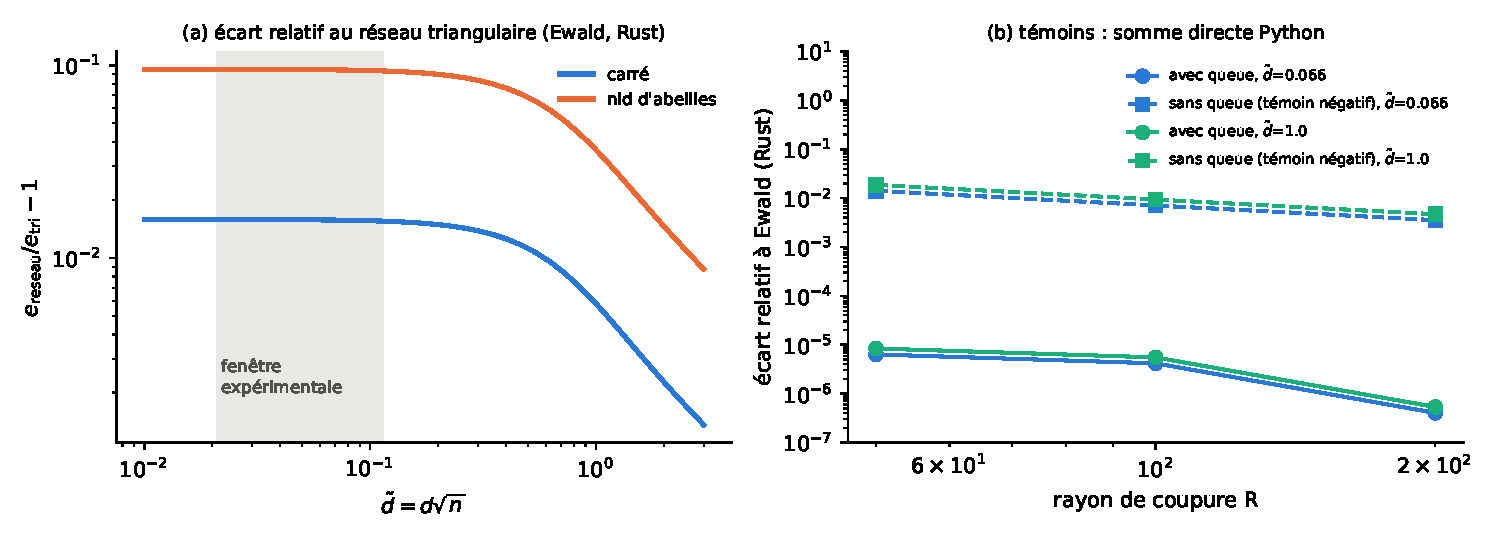
\includegraphics[width=\textwidth]{ch5_U1_dipolar.pdf}
\caption{U1 \tierX. (a) Relative gap of the square and honeycomb lattices to the triangular lattice (exact Ewald
energies, rusty-SUNDIALS), as a function of $\tilde d$. The grey band is the experimental window deduced from
JARVIS-DFT. (b) Controls: a direct sum in Python, \emph{with} the exact uniform tail, converges to the
Ewald value; \emph{without} the tail (negative control), the error stays of order $10^{-2}$.}\label{ch5:fig:U1}
\end{figure}

\paragraph{The result \tierX.} Over the whole grid, both gaps remain positive:
\begin{itemize}
\item $e_\mathrm{square}/e_\mathrm{tri}-1$ decreases from $1.58\times10^{-2}$ to $1.36\times10^{-3}$;
\item the honeycomb gap decreases from $9.53\times10^{-2}$ to $8.75\times10^{-3}$.
\end{itemize}
Converted to energy (unscreened, to be divided by $\varepsilon_r$), the square-minus-triangular gap is
$0.0014$, $0.044$ and $0.224$~meV per exciton at the three densities. These values are interpolated on the grid;
the paper gave $0.223$~meV at the nearest grid point. This is one to five orders of magnitude below the
depth of moiré wells, ``tens to 100~meV''~\cite{ch5:wang}. In the published study, none
of the 21 competitors relaxed by CVODE went below the triangular lattice~\cite{ch2dip}.

\paragraph{The controls.}
\begin{itemize}
\item \emph{Positive.} An independent direct Python sum, plus the exact tail $2\pi/(\sqrt{R^2+\tilde
d^2}+R)$, recovers Rust's Ewald value. The relative deviation is $4.0\times10^{-7}$ at $\tilde d=0.066$ and
$5.3\times10^{-7}$ at $\tilde d=1$, for $R=200$. The Ewald energy is independent of the splitting
parameter $\eta$ to within $9.0\times10^{-15}$.
\item \emph{Negative.} Without the tail, the same sum is off by $3.5\times10^{-3}$ and $4.7\times10^{-3}$ at
$R=200$, and by $1.4\times10^{-2}$ at $R=50$.
\item \emph{Negative.} The script checks that $h_d(d^2)<0$ for $d=0.5$, $1$ and $2$. The square and honeycomb
lattices keep a higher energy at each of the 41 grid points.
\end{itemize}
We also reran, separately, two relaxations of the published study at $\tilde d=0.066$ (command
\texttt{dipolar\_crystal main <dir> 0.066 1 0 1}, about 8~minutes on two cores):
\begin{itemize}
\item the uniform start \texttt{uniform\_00} ends at a relative gap of $1.382373\times10^{-3}$, with 4 defects;
\item the incommensurate box, a negative control, ends at $2.000407\times10^{-3}$, with 8 defects.
\end{itemize}
Both values match the record, digit for digit.

\paragraph{What this does not show.}
\begin{itemize}
\item The model is classical, at zero temperature, with rigid dipoles and no screening: no
Rytova--Keldysh form, no moiré potential, no kinetic energy. In the experimental window, real excitons
form a quantum gas, not a classical crystal~\cite{ch5:wang}.
\item The JARVIS $d$ is a proxy: that of two homogeneous stackings, not that of a heterobilayer. The
dataset fixes the scale of $\tilde d$; it does not test the theorem.
\item No relaxation proves optimality: 21 trials do not cover the infinitely many configurations.
\end{itemize}

% =====================================================================================================
\section{U2 -- Planar Yukawa crystals: dusty plasmas and colloids}\label{ch5:U2}

\paragraph{The question.} In a laboratory dusty plasma, charged microparticles levitate in a plane.
They repel each other through a Coulomb potential screened by the ions, $V(r)=Q^2e^{-r/\lambda_D}/r$. Charged
colloids in suspension behave in the same way. At fixed density, which configuration minimizes the energy?
Hexagonal crystals are observed; can this be proved within this model?

\paragraph{The theorem and its tier.} With $t=r^2$ and $\kappa=\ell/\lambda_D$, where $\ell$ is the length
scale set by the density, $g_\kappa(t)=e^{-\kappa\sqrt t}/\sqrt t$. The human proof \tierC{} proceeds in
three steps:
\begin{itemize}
\item $t\mapsto\sqrt t$ is a Bernstein function and $x\mapsto e^{-\kappa x}$ is completely monotone,
so their composite $e^{-\kappa\sqrt t}$ is completely monotone (this is the CM\,$\circ$\,Bernstein rule of the P3 library, doi:10.5281/zenodo.23653842);
\item $t^{-1/2}$ is completely monotone;
\item a product of two completely monotone functions is again completely monotone (Leibniz rule: every term has the
right sign).
\end{itemize}
Lean checks it \tierA{} (Lean 4.34.1), conditionally on the upstream result:
\begin{leanbox}[: \texttt{formal\_cert/Autoresearch/Yukawa.lean} (statements)]
\begin{lstlisting}[language=Lean]
theorem yukawa_admissible {κ : ℝ} (hκ : 0 < κ) : AdmissiblePotential (g κ)
theorem triangular_yukawa_optimal {κ : ℝ} (hκ : 0 < κ) (C : Set Plane) (hC : LocallyFinite C)
    (hdens : DensityOne C) : latticeEnergy (g κ) ≤ energy (g κ) C
theorem latticeEnergy_yukawa_lt_top {κ : ℝ} (hκ : 0 < κ) : latticeEnergy (g κ) < ⊤
\end{lstlisting}
\end{leanbox}
The module \texttt{YukawaMix.lean} extends the result to every finite mixture $\sum_iw_ie^{-\kappa_ir}/r$ with weights
$w_i\ge0$. The formal negative control is the signed mixture $g_1-2g_2$: it equals $2e^{-1/2}-4e^{-1}\approx-0.2585$
at $t=\tfrac14$, so it is not admissible. The theorem does not apply to it, which does not mean that
optimality fails. Paper: doi:10.5281/zenodo.23646105~\cite{ch2yuk}.

\begin{uniremark}\tierL{} By Bernstein's theorem, a function $g$ on $(0,\infty)$ is completely monotone if and only if
$g(t)=\int_{[0,\infty)}e^{-ts}\,d\mu(s)$ for a positive Borel measure $\mu$~\cite{bernstein,widder}. In this language
the three steps above are closure properties of Laplace transforms of positive measures: a product corresponds to the
convolution of the measures, and composing with a Bernstein function corresponds to subordination. For instance
$e^{-\kappa\sqrt t}$ is the Laplace transform of the one-sided $\tfrac12$-stable (Lévy) density (standard).
\end{uniremark}

\paragraph{The data.} On 2026-10-25, a search of the Hub (\emph{dusty plasma}, \emph{complex plasma},
\emph{colloid}, \emph{yukawa}, \emph{wigner crystal}) found no dataset of grain or colloid
positions~\cite{ch2yuk}. This is an absence observed by search, not a proof. The disordered
initial conditions therefore come from an entirely different field, catalysis:
\begin{itemize}
\item identifier \texttt{colabfit/OC20\_IS2RES\_val\_id}, licence CC-BY-4.0~\cite{ch5:oc20};
\item file \texttt{co/co\_10.parquet}, 142\,986\,687 bytes; its local sha256 equals the Hub's LFS hash at
revision \texttt{6a1dfef12aec878b4cda99edd54b16a6a254e135};
\item adsorbate structures, rotated in 3D, projected onto the plane, rescaled and filtered by a
minimum distance.
\end{itemize}
The script checks the sha256 and finds in the file the OC20 configuration identifiers listed in
\texttt{provenance.json}. These data provide realistic-looking \emph{disorder}, nothing more: molecules
adsorbed on a catalyst have nothing to do with screened charged grains.

\paragraph{The numerical method.} The module \texttt{exact.rs} of \texttt{qf-yukawa-crystal} has three parts:
\begin{itemize}
\item lattice sums of the \emph{untruncated} potential, with a rigorous bound on the tail;
\item an independent Ewald decomposition;
\item a periodic box summing all images within radius $R$, with analytic energy, force and
Hessian.
\end{itemize}
The tail bound relies on Voronoi cells: for decreasing $V$, the tail beyond $R$ is at most
$(\pi/A)\bigl(1+\delta/(R-2\delta)\bigr)e^{-\kappa(R-2\delta)}/\kappa$. The relaxation (\texttt{exact-relax}) uses
CVODE: BDF, Jacobian equal to minus the Hessian, $\mathrm{rtol}=10^{-10}$, $\mathrm{atol}=10^{-12}$ and
force tolerance $10^{-9}$. Each minimum is checked through the spectrum of the Hessian. This computation corrects a
published erratum: an earlier version truncated the potential at $r_c=8$ with a force shift, and this truncated
potential is no longer completely monotone.

\paragraph{The script.} \texttt{code/ch5\_U2\_yukawa.py OUTPUT}:
\begin{enumerate}
\item it copies the initial conditions into a working crate;
\item it runs \texttt{yukawa\_crystal exact-refs}, then \texttt{exact-relax 2 1 0 0}. At $\kappa=2$, this means
three relaxations of about 1 to 2~minutes each on two cores: an OC20 start, a uniform start and an
incommensurate box;
\item it runs the controls and plots \texttt{figures/ch5\_U2\_yukawa.pdf}.
\end{enumerate}
The option \texttt{--skip-relax} rereads the record instead of rerunning the relaxations.

\begin{figure}[ht]\centering
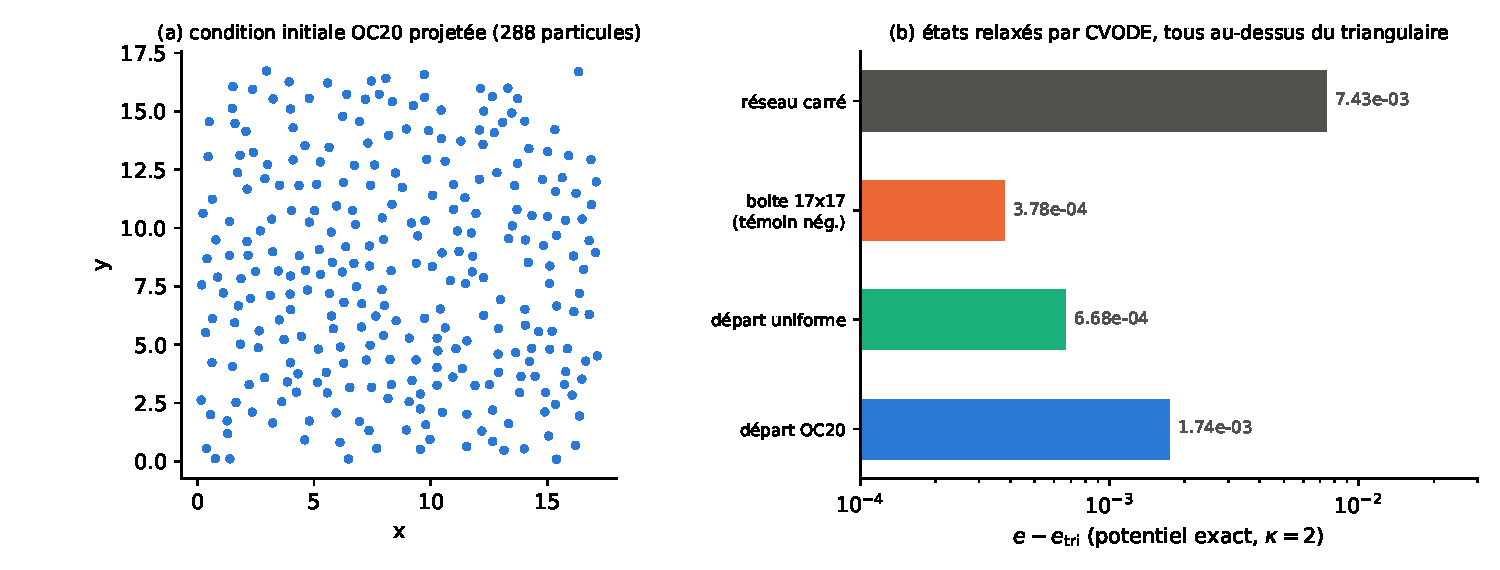
\includegraphics[width=\textwidth]{ch5_U2_yukawa.pdf}
\caption{U2 \tierX. (a) Initial condition drawn from OC20 (288 particles in a box that exactly contains the
triangular lattice). (b) Gap $e-e_\mathrm{tri}$ of the states relaxed by CVODE under the exact potential
($\kappa=2$), to be compared with the gap of the square lattice. No state lies below the triangular
lattice.}\label{ch5:fig:U2}
\end{figure}

\paragraph{The result \tierX.} Energies per particle at density one, in the $\tfrac12\sum$ convention:

\begin{center}\small
\begin{tabular}{lllll}\toprule
$\kappa$ & triangular (exact) & square (exact) & gap & truncated--exact (tri.)\\\midrule
1 & 1.6253213396063 & 1.6348554953172 & $9.534\times10^{-3}$ & $-1.771\times10^{-2}$\\
2 & 0.3935428489324 & 0.4009742487651 & $7.431\times10^{-3}$ & $-9.48\times10^{-6}$\\
\bottomrule\end{tabular}
\end{center}
The tail bound is at most $5.6\times10^{-17}$ ($\kappa=1$, $R=40$) and $1.2\times10^{-16}$ ($\kappa=2$,
$R=20$). The three relaxations at $\kappa=2$ converge, with no negative mode of the Hessian:
\begin{itemize}
\item OC20 start: gap $1.742\times10^{-3}$, 24 defects, 157 CVODE steps;
\item uniform start: gap $6.68\times10^{-4}$, 4 defects;
\item incommensurate $17\times17$ box: gap $3.78\times10^{-4}$, 4 defects.
\end{itemize}
In the full study, none of the 24 stages relaxed under the exact potential went below the triangular
lattice~\cite{ch2yuk}.

\paragraph{The controls.}
\begin{itemize}
\item \emph{Positive.} A direct Python lattice sum recovers Rust's exact values to within
$1.4\times10^{-16}$ in relative terms at most (the required threshold is $10^{-12}$). In addition, the periodic box containing the perfect lattice equals the infinite
sum to within $2.2\times10^{-16}$.
\item \emph{Negative.} The energies truncated at $r_c=8$ miss the exact value by far more than $10^{-9}$. The
$17\times17$ box, which cannot contain the triangular lattice, stays above. The perfect square lattice is a saddle
of the exact potential, with 72 negative modes at $\kappa=2$ and 64 at $\kappa=1$~\cite{ch2yuk}.
\end{itemize}

\paragraph{What this does not show.}
\begin{itemize}
\item The OC20 data contain no plasma physics: they serve only as initial disorder.
\item The potential $K_0(\kappa r)$, the 2D Debye--Hückel Green's function, is not treated. Neither are mixtures with
negative weights, finite temperature or uniqueness.
\item The annealing was not redone with the exact potential.
\end{itemize}

% =====================================================================================================
\section[U3 -- Superfluid helium and the Feynman--Bijl test]{U3 -- Superfluid helium: structure factor and the Feynman--Bijl test}\label{ch5:U3}

\paragraph{The question.} X-ray or neutron diffraction measures the static structure factor $S(k)$
of a liquid. For a weakly interacting Bose gas, Bogoliubov theory predicts
$S_B(k)=\varepsilon_0(k)/\varepsilon_B(k)$, with $\varepsilon_0=\hbar^2k^2/2m$. Can one say, \emph{from
$S(k)$ alone}, that superfluid helium-4 is not a Bogoliubov gas?

\paragraph{The theorem and its tier.} Set $k^*=2mc/\hbar$, where $c$ is the speed of sound. Then
$S_B(k)=k/\sqrt{k^{*2}+k^2}$ and
\[S_B(k)\le\sqrt{\frac{k}{2k^*}},\qquad\text{with equality if and only if }k=k^* .\]
\begin{humanproof}
Both sides are positive; we compare their squares. $S_B^2\le k/2k^*$ is equivalent to
$2k^*k\le k^{*2}+k^2$, that is, to $(k-k^*)^2\ge0$.
\end{humanproof}
\begingroup\sloppy The statement is \tierAs{}, in the QuantumFluids environment (Lean v4.34.0-rc2; no \texttt{leanchecker} replay recorded for this environment), under the name
\lean{sBog_le_sqrt}. Both controls are checked by the kernel: the test fires on the free value $S=1$
for every $0<k<2k^*$ (\lean{free_S_one_violates}), and never fires on $S_B$. The corollary
\lean{not_bogoliubov_of_structure_factor} gives the ``diffraction test'': if a measured $S$ exceeds
$\sqrt{k/2k^*}$, this $S$ is not the structure factor of a Bogoliubov gas with that speed of sound.
The Feynman--Bijl argument relates $S$ to the excitation energy, $\varepsilon(k)\le\hbar^2k^2/(2mS(k))$. Its
single-mode core is formalized in Lean 4.34.1, with the f-sum rule identity taken as a
\emph{hypothesis}. Papers: doi:10.5281/zenodo.23646117~\cite{ch3-bsk} and
doi:10.5281/zenodo.23653846~\cite{ch3-fb}.\par\endgroup

\paragraph{The data (not Hugging Face).} No structure-factor dataset exists on the Hub: the
searches for these two papers found none. We use Table~14.1 of the compilation by Donnelly and
Barenghi~\cite{ch3-db}, in its web edition (assumed, without verification, to reproduce the 1998 table):
\begin{itemize}
\item 99 points with $Q>0$: 49 X-ray points (Robkoff--Hallock) and 50 neutron points (Svensson et al.);
\item temperatures from 1.4 to 4~K, no error bars printed.
\end{itemize}
This is a secondary source at \tierL{}. The extracted file is
\url{papers/prog_superfluid_structure_factor/data/he4_Sk_donnelly_table14_1.csv}. We take
$c=238.3\pm0.1$~m/s~\cite{ch3-godfrin}, whence $k^*=3.00379$~\AA$^{-1}$ (between 3.0025 and 3.0051).

\paragraph{The method.} For each point, the verdict is:
\begin{itemize}
\item \textsc{compatible} if $S\le\sqrt{Q/2k^*}$;
\item \textsc{refuted} if $S-\sqrt{Q/2k^*}>\Delta$;
\item \textsc{undecided} otherwise.
\end{itemize}
The threshold $\Delta=0.082$ is the gap between the maxima of the two datasets in the table. This threshold was fixed after the fact; it
was not preregistered. On the rusty-SUNDIALS side, the module \texttt{linear\_response} of \texttt{qf-gpe2d} gives a
cross-check: one excites the Gross--Pitaevskii ground state ($32\times32$ grid, Strang split step),
measures the frequency of the response, and derives $\varepsilon_B(k)$ and $S(k)$ from it.

\paragraph{The script.} \texttt{code/ch5\_U3\_helium.py OUTPUT [--gpe-json FILE]} applies the test and runs the
controls. If it is given the output of the \texttt{bogoliubov\_dispersion} example of \texttt{qf-gpe2d}, it also plots
the linear response.

\begin{figure}[ht]\centering
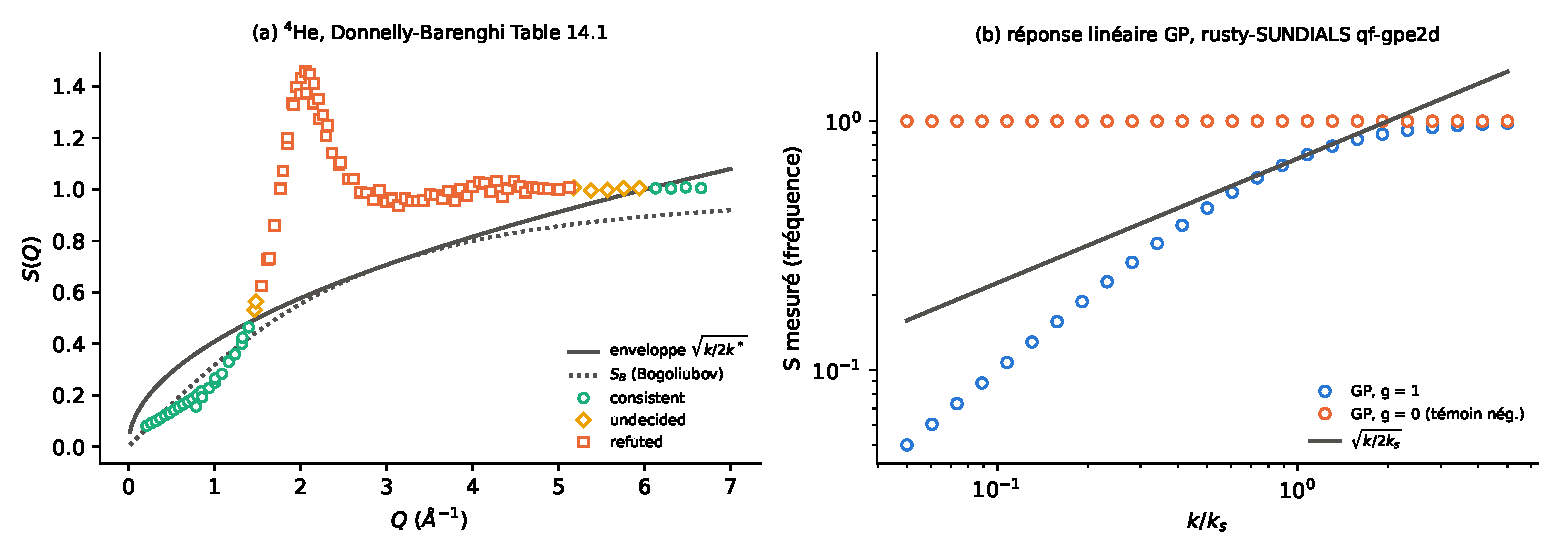
\includegraphics[width=\textwidth]{ch5_U3_helium.pdf}
\caption{U3. (a) $S(Q)$ of helium-4 (Table~14.1, Tier~L) against the envelope $\sqrt{Q/2k^*}$ (solid line) and
$S_B$ (dotted); the colour gives the verdict (arithmetic, Tier~X). (b) Gross--Pitaevskii linear response
computed by rusty-SUNDIALS \tierX{}: measured $S$ for $g=1$ below the envelope, control $g=0$ ($S=1$) above it for
$k<2k_s$.}\label{ch5:fig:U3}
\end{figure}

\paragraph{The result.} Of the 99 points, 29 are compatible, 7 undecided and 63 refuted. The 21 points of the
peak and roton region ($1.7\le Q\le2.4$~\AA$^{-1}$) are all refuted: there $S$ exceeds the envelope by a factor of
1.62 to 2.49. The helium-4 measurements are therefore not the $S$ of a Bogoliubov gas with the same speed of sound. This
textbook result is now a consequence of a checked statement and a published table.

We reran the \texttt{bogoliubov\_dispersion} example (10~min 24~s on one core), and its output is
bit-for-bit identical to the record. In this Gross--Pitaevskii linear response \tierX{}:
\begin{itemize}
\item the frequency measured for $g=1$ recovers $\varepsilon_B$ to within $4.1\times10^{-5}$ in relative terms;
\item the measured $S$ stays below the envelope, since $\max(S/\sqrt{k/2k_s})-1=-1.4\times10^{-3}$;
\item the control $g=0$, a free gas where $S=1$, exceeds the envelope at the 20 wavenumbers of the sweep with
$k<2k_s$.
\end{itemize}

\paragraph{The controls.}
\begin{itemize}
\item \emph{Positive.} $S_B$ fires the test at none of the 99 points.
\item \emph{Negative.} The free value $S=1$ fires it at 95 of the 95 points with $Q<2k^*$.
\end{itemize}
Both controls are also Lean theorems.

\paragraph{What this does not show.}
\begin{itemize}
\item The physical conclusion is conditional \tierC{}: the table was measured between 1.4 and 4~K, not at
$T=0$. We have not quantified how the peak of $S$ varies with temperature.
\item A compatible point is not \emph{confirmed} ``Bogoliubov'': the envelope is only an upper
bound, and at small $k$ it has very little testing power.
\item Beyond the peak, the failure resembles that of the control $S=1$: this is no longer roton physics.
\end{itemize}

% =====================================================================================================
\section[U4 -- Turbulence: enstrophy bound]{U4 -- Turbulence: enstrophy bound in the shell model \texorpdfstring{$\sigma=3$}{sigma=3}}\label{ch5:U4}

\paragraph{The question.} Shell models replace a turbulent velocity field by one complex amplitude
$v_n$ per octave of wavenumbers, $k_n=2^n$, $n=0,\dots,N+1$. Neighbouring shells exchange energy through a
quadratic term. Add a dispersive term $-i\omega_nv_n$ with $\omega_n=Dk_n^3$ (``$\sigma=3$''). Can one
bound the enstrophy $\Omega=\tfrac12\sum k_n^2|v_n|^2$, which measures the small scales, along \emph{every}
trajectory and for \emph{every} truncation $N$?

\paragraph{The theorem and its tier.} The model conserves two quantities:
\begin{itemize}
\item the ``mass'' $S=\sum|v_n|^2=2E$;
\item the invariant $H=\sum2^{-n}\omega_n|v_n|^2+\sum2^{-n}k_n\,\mathrm{Im}(\bar v_n^{\,2}v_{n+1})$, for \emph{every}
real dispersion law.
\end{itemize}
For $\omega_n=Dk_n^3$, the quadratic part of $H$ equals exactly $2D\Omega$. The cubic part $C$ satisfies
$|C|\le S^{3/2}$.
\begin{humanproof}
Write $H_3(0)$ for the value of $H$ at time $0$. Since $H$ is conserved, $2D\Omega(t)=H_3(0)-C(t)$. Hence
$2D\Omega(t)\le H_3(0)+|C(t)|\le H_3(0)+S(t)^{3/2}$. Since $S$ is conserved,
$2D\Omega(t)\le H_3(0)+(2E(0))^{3/2}$.
\end{humanproof}
Lean checks all of this \tierAs{} (Lean v4.34.0-rc2, the project's Mathlib; no \texttt{leanchecker} replay):
\begin{itemize}
\item the rate identity of $H$ along the vector field;
\item the chain rule;
\item the constancy of $H$ and $S$ on $[0,T]$;
\item the bound \lean{enstrophy_bound_along_flow}, for every trajectory on $[0,T]$ and every $N$.
\end{itemize}
\begingroup\sloppy The statement assumes that the trajectory exists and is differentiable at every instant of $[0,T]$: existence is
a \emph{hypothesis}, not a theorem. The level $N$ stays fixed. Paper: doi:10.5281/zenodo.23646111~\cite{ch5:sigma3}.\par\endgroup
\paragraph{The data.} The Well~\cite{ch5:thewell} contains large-scale fluid simulations. We
use:
\begin{itemize}
\item identifier: \url{polymathic-ai/turbulent_radiative_layer_2D};
\item revision \texttt{2ee7756575ff6f90981d0308cbcb6a2ab5995bdc}, licence CC-BY-4.0 according to the card;
\item the file\\ \url{data/test/turbulent_radiative_layer_tcool_0.32.hdf5},\\ sha256 \texttt{06cbd36c\dots f747},
checked by the script.
\end{itemize}
These are Athena++ simulations of the 2D compressible Euler equations with radiative cooling.

The spectrum is built as follows, for four developed snapshots (indices 25, 50, 75 and 100):
\begin{enumerate}
\item take the FFT of the velocity along the periodic axis $x$, without the mode $k_x=0$;
\item average over $y$;
\item sum $k_x\in[2^n,2^{n+1})$ into shell $n=0,\dots,5$.
\end{enumerate}
This step reads the HDF5 file with \texttt{h5py}, which is absent from AutoevolveAI's \texttt{.venv} environment: the script
therefore rereads the file \texttt{well\_amps.txt} that these steps produced. The $\log_2$ slopes of the spectra are
$-2.13$, $-1.56$, $-1.79$ and $-1.81$~\cite{ch5:sigma3}.

\paragraph{The numerical method.} The module \texttt{sigma.rs} of \texttt{qf-shell-cascade} integrates the model with CVODE:
\begin{itemize}
\item BDF, analytic Jacobian, $\mathrm{atol}=10^{-3}\,\mathrm{rtol}$, $D=0.05$;
\item suprema taken at CVODE's internal step points, without interpolation.
\end{itemize}
The program \texttt{sigma3\_study full} runs five blocks in sequence:
\begin{itemize}
\item a positive control, the convergence of conservation with the tolerance;
\item a negative control, a perturbed coupling;
\item a sweep of truncations $n_{\max}\le7$;
\item the comparison $\sigma=2$ versus $\sigma=3$ on data concentrated in the last shell;
\item 24 trajectories initialized from the moduli of The Well, with two draws of random phases and
$n_{\max}=5,6,7$.
\end{itemize}

\paragraph{The script.} \texttt{code/ch5\_U4\_shell.py OUTPUT} runs \texttt{sigma3\_study full} (from 2.5 to 6~minutes
depending on the machine's load), checks the criteria and plots \texttt{figures/ch5\_U4\_shell.pdf}.

\begin{figure}[ht]\centering
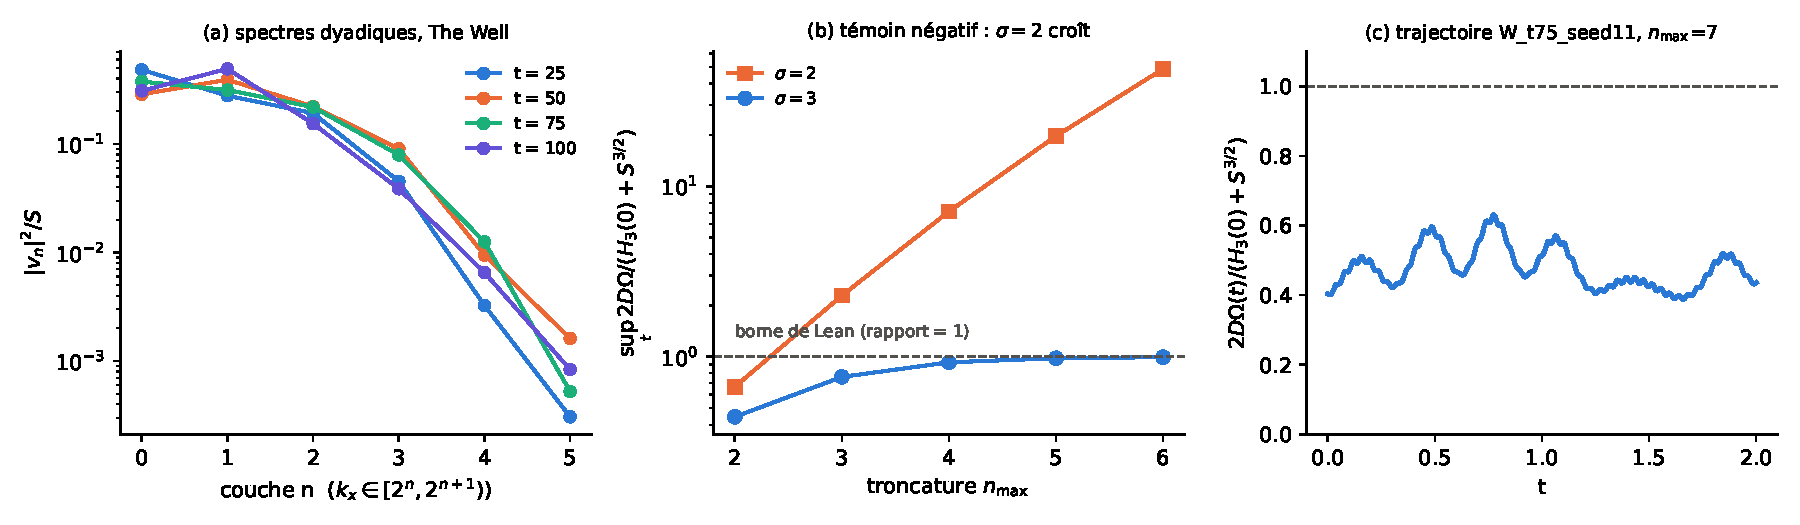
\includegraphics[width=\textwidth]{ch5_U4_shell.pdf}
\caption{U4 \tierX. (a) Dyadic spectra of four snapshots of The Well, normalized to $S=1$. (b) Ratio
$\sup_t2D\Omega/(H_3(0)+S^{3/2})$ on data concentrated in the last shell: it stays below 1 for
$\sigma=3$ and grows with $n_{\max}$ for $\sigma=2$ (negative control). (c) The ratio along the trajectory
initialized from The Well that comes closest to the bound.}\label{ch5:fig:U4}
\end{figure}

\paragraph{The result \tierX.} The 17 $\sigma=3$ trajectories of the sweep and of the comparison all stay below the
bound. The ratio $\sup_t2D\Omega(t)/(H_3(0)+S(0)^{3/2})$ is at most 0.995; this maximum is reached on data
concentrated in the last shell, where the ratio tends to 1 as $n_{\max}$ grows (0.444, 0.762, 0.928, 0.981
and 0.995 for $n_{\max}=2,\dots,6$). The 24 trajectories initialized from The Well also stay below the bound, with
a ratio of at most 0.631. Their relative drifts are at most $2.4\times10^{-8}$ on $S$ and $1.2\times10^{-6}$
on $H$. The recomputed file \texttt{sigma3\_study.json} is identical to the record of
the paper~\cite{ch5:sigma3}, up to run times.

\paragraph{The controls.}
\begin{itemize}
\item \emph{Positive.} With the true coupling, the drift of $H$ decreases with the tolerance. For $n_{\max}=4$, it
is $2.6\times10^{-5}$, $8.6\times10^{-7}$ and then $1.9\times10^{-8}$ for
$\mathrm{rtol}=10^{-6},10^{-8},10^{-10}$.
\item \emph{Negative.} If the coupling leaving shell~1 is perturbed by $10^{-2}$, the drift of $H$ stays
stuck near $2.3\times10^{-3}$ ($n_{\max}=4$) and $5.4\times10^{-3}$ ($n_{\max}=6$), whatever the
tolerance. Conservation therefore comes from the structure of the model, not from the accuracy of the solver.
\item \emph{Negative.} For $\sigma=2$, the same inequality has no proof, and the ratio is 0.667, 2.29,
7.11, 19.7 and then 48.8 for $n_{\max}=2,\dots,6$. It exceeds 1 from $n_{\max}=3$ on and grows faster than an
exponential of ratio 2 over this range (Figure~\ref{ch5:fig:U4}b).
\end{itemize}

\paragraph{What this does not show.}
\begin{itemize}
\item The Well data give a realistic spectral shape, and nothing else. The flow is compressible
and cooled; it does not conserve energy. The spectrum is one-dimensional and carries no phases (they are
drawn at random).
\item Over $T=2$, the upper shells, initially empty, barely fill up. These trajectories therefore do not probe
the dependence on $N$.
\item There is no statement for infinitely many shells. Uniformity in $N$ requires initial data whose
$\Omega(0)$ and $S(0)$ are bounded uniformly in $N$ (a Tier C corollary).
\item BDF damping makes $S$ drift downwards. The observed margins far exceed these drifts,
but the simulation does not replace the theorem.
\end{itemize}

% =====================================================================================================
\section{U5 -- Genetics: fixation of a mutation}\label{ch5:U5}

\paragraph{The question.} A population has $N$ individuals, $i$ of whom carry a mutation of relative
fitness $r$. What is the probability that the mutation eventually takes over the whole population
(\emph{fixation})? And what becomes of this probability when the population lives on a graph?

\paragraph{The Moran model.} At each step, one individual is chosen to reproduce with probability
proportional to its fitness, and one individual drawn uniformly at random dies. The number of mutants is a
birth--death chain on $\{0,\dots,N\}$. Its up and down probabilities are
\[p_i=\frac{ri}{ri+N-i}\cdot\frac{N-i}{N},\qquad q_i=\frac{N-i}{ri+N-i}\cdot\frac iN,\qquad\text{hence } p_i=r\,q_i .\]

\paragraph{The theorem and its tier.} Write $\varphi_i$ for the fixation probability starting from $i$ mutants. The
first-step equation gives $p_i(\varphi_{i+1}-\varphi_i)=q_i(\varphi_i-\varphi_{i-1})$, with $\varphi_0=0$ and
$\varphi_N=1$.
\begin{humanproof}[Human proof (formula)]
Set $\delta_i=\varphi_{i+1}-\varphi_i$. The equation gives $\delta_i=\delta_{i-1}/r$, hence $\delta_i=r^{-i}\delta_0$
and $\varphi_i=\delta_0S_i$, where $S_i=\sum_{k<i}r^{-k}$. The condition $\varphi_N=1$ fixes
$\delta_0=1/S_N$. For $r\ne1$, we obtain
\[\varphi_i=\frac{S_i}{S_N}=\frac{1-r^{-i}}{1-r^{-N}} .\]
For $r=1$, we obtain $\varphi_i=i/N$.
\end{humanproof}
Programme P7 checks more \tierA{} (Lean 4.34.1). It proves the \emph{absorption limit},
$P^n(i,N)\to(1-r^{-i})/(1-r^{-N})$, and uniqueness: every function that is harmonic in the interior with values $0$ and
$1$ on the boundary equals $\varphi$. Programme N4 proves the isothermal theorem (birth--death): on a
strongly connected graph whose replacement matrix is doubly stochastic, fixation follows the same law.
\begin{leanbox}[: \texttt{PopGen/MoranFixation.lean} and \texttt{EvoGraph/BirthDeath.lean} (statements)]
\begin{lstlisting}[language=Lean]
theorem moran_fixation_limit_closed {N : ℕ} {r : ℝ} (hN : 0 < N) (hr : 0 < r) (hr1 : r ≠ 1)
    (i : Fin (N + 1)) :
    Tendsto (fun n => kPow (moranP N r) n i (Fin.last N)) atTop
      (𝓝 ((1 - r⁻¹ ^ (i : ℕ)) / (1 - r⁻¹ ^ N)))
theorem moran_fixation_unique {N : ℕ} {r : ℝ} (hN : 0 < N) (hr : 0 < r) {g : Fin (N + 1) → ℝ}
    (hg : InteriorHarmonic (moranP N r) g) (g0 : g 0 = 0) (g1 : g (Fin.last N) = 1) :
    ∀ i, g i = moranFix N r i
theorem isothermal_fixation {W : Fin n → Fin n → ℝ} {r : ℝ} (hn : 0 < n) (hr : 0 < r)
    (hW : Isothermal W) (hsc : StronglyConnected W) (S : Finset (Fin n)) :
    Tendsto (fun t => sPow (bdK (fun _ => 1) W r) t S univ) atTop (𝓝 (moranFix n r S.card))
\end{lstlisting}
\end{leanbox}
The general absorption theorem of P7 and the single-mutant version of the isothermal theorem reappear under
the names \lean{KAL} and \lean{ILENE} in Section~\ref{ch5:acronymes}.

\begin{uniremark}\tierL{} For a finite absorbing Markov chain, the absorption probabilities form the unique bounded
solution of the first-step equations that is harmonic at the transient states and takes the prescribed boundary values;
equivalently, if $h$ is such a solution then $h(X_n)$ is a bounded martingale and the optional stopping theorem at the
absorption time gives $h(i)=\mathbb P_i(\text{absorption at }N)$~\cite{app:norris,app:williams}.
\end{uniremark}

The number of mutants on a graph is \emph{not} a Markov chain in general. On the 4-cycle, the one-step up
probability depends on the configuration, $1/3$ versus $2/3$ at $r=2$. What is true, and proved, is the bias
\emph{per configuration} $P^+=r\,P^-$. On the star with $n=3$ nodes, which is not isothermal, the limits are
$5/12$, $2/3$ and $7/12$, against $4/7$ for Moran. Papers: doi:10.5281/zenodo.23653850~\cite{ch4:P7} and
doi:10.5281/zenodo.23660071~\cite{ch4:N4}.

\paragraph{The data: what they illustrate, and what they do not estimate.} The author's Genetic repository
uses the datasets \texttt{katarinagresova/Genomic\_Benchmarks\_*}~\cite{ch5:gb}. We take one of them:
\begin{itemize}
\item identifier \url{katarinagresova/Genomic_Benchmarks_demo_coding_vs_intergenomic_seqs}, revision
\texttt{85458172cab6cffad46cb172e64ca94780506ed6};
\item the test split, \url{data/test-00000-of-00001-6fccc31405110e30.parquet}, 2\,456\,511 bytes, sha256
\texttt{dfe13715\dots 9afe}.
\end{itemize}
The card states \emph{no} licence and does not say what the labels 0 and 1 mean. We
reproduce only aggregate statistics, and the licence of the upstream package has not been checked.

The script counts 25\,000 sequences, 12\,500 per label, all of length 200, with no symbol other than A, C, G and T.
The GC fraction is 0.5381 for label~0 and 0.4004 for label~1 (Figure~\ref{ch5:fig:U5}c).

This is what sequence data look like: a point mutation is the replacement of one letter.
\textbf{But this dataset estimates no fitness $r$}, and nothing in this chapter derives one from it. The values of $r$
used below (0.8, 1, 1.2, 1.5 and 2) are \emph{chosen}, not measured.

\paragraph{The numerical method.} The crate \texttt{qf-popgen} writes the absorbing chain as a linear
differential equation, $\dot\pi=\pi(P-I)$: this is the forward Kolmogorov equation of the uniformized chain. It
integrates it with CVODE (BDF, exact Jacobian, $\mathrm{rtol}=10^{-11}$, $\mathrm{atol}=10^{-15}$). An
\emph{absorption certificate} rejects any doubtful run, in a ``fail-closed'' spirit (rejecting by default): a run is
accepted only if five conditions hold:
\begin{itemize}
\item the kernel is stochastic and absorbing;
\item the total mass is conserved;
\item no component becomes negative;
\item the interior mass has dropped below $10^{-9}$;
\item the mass at $N$ equals the target to within $10^{-8}$.
\end{itemize}
The passage from the differential equation to the $n$-step kernel (a Poisson mixture) is not formalized.

Finally, \textbf{LeanFlow} certifies a computed number. Its function \texttt{lean.certify} accepts a claim about
rational enclosures and translates it into a statement about integers. The tactic \texttt{decide\_kernel}
(\lean{decide +kernel}) has this statement decided by the kernel, with no extra axiom. LeanFlow then audits
\texttt{\#print axioms}, and an exact Python oracle must return the same verdict.

\paragraph{The script.} \texttt{code/ch5\_U5\_fixation.py OUTPUT}:
\begin{enumerate}
\item it downloads the file at the pinned revision, checks its digest and computes the statistics;
\item it runs \texttt{fixation\_ode};
\item it compares the CVODE values with the exact fractions;
\item it submits five claims to LeanFlow (Lean 4.34.1, core only);
\item it plots \texttt{figures/ch5\_U5\_fixation.pdf}.
\end{enumerate}
It takes about twenty seconds.

\begin{figure}[ht]\centering
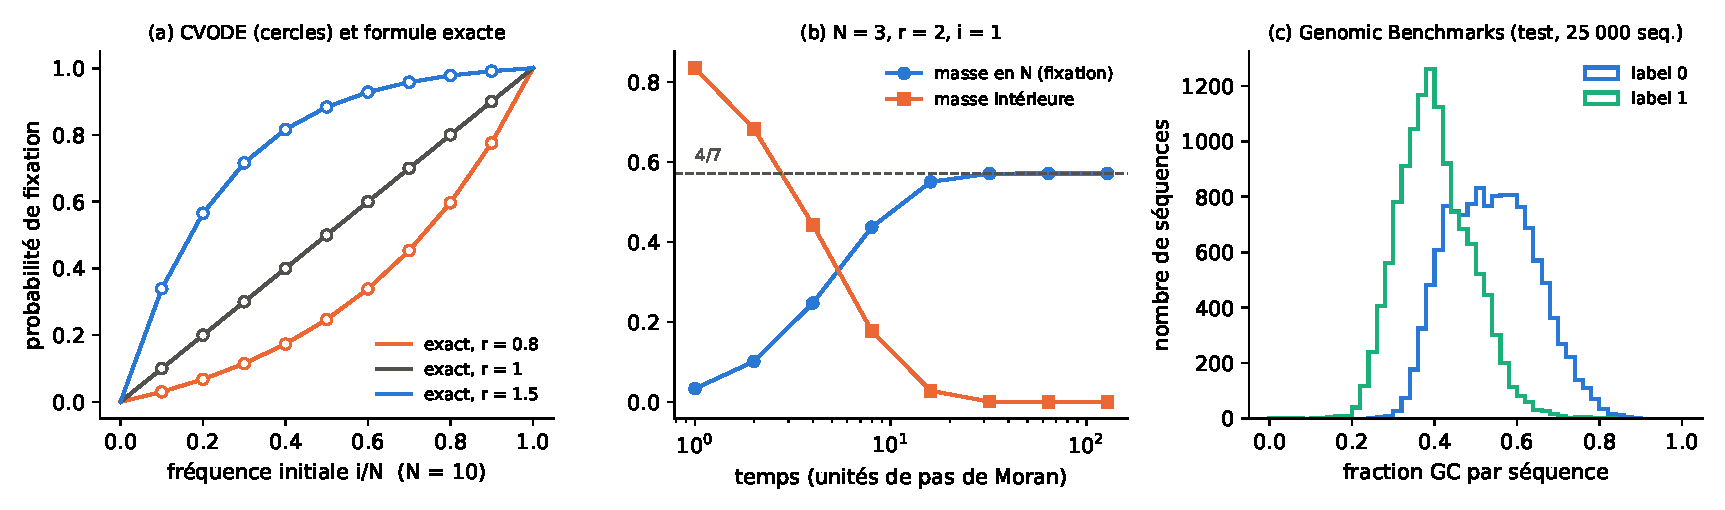
\includegraphics[width=\textwidth]{ch5_U5_fixation.pdf}
\caption{U5. (a) Fixation probability for $N=10$: CVODE (circles, \tierX) and exact formula (lines), for
$r=0.8$, $1$ and $1.5$. (b) CVODE trajectory for $N=3$, $r=2$, $i=1$: the mass absorbed at $N$ tends to
$4/7$, the interior mass dies out. (c) GC fraction of the 25\,000 test sequences of Genomic Benchmarks; this
dataset illustrates sequence data and estimates no fitness.}\label{ch5:fig:U5}
\end{figure}

\paragraph{The result.} \texttt{fixation\_ode} produces 115 rows: 106 accepted runs and 9 negative controls
rejected, without a single exception. Over the accepted Moran runs, the maximal deviation between CVODE and the exact
fraction $S_i/S_N$ is $3.1\times10^{-10}$ \tierX.

For $N=3$, $r=2$, $i=1$, CVODE gives $0.5714285714284759$, a deviation of $9.55\times10^{-14}$ from $4/7$.
LeanFlow then certifies two claims \tierA{} (on the arithmetic statement only, empty axiom list; each claim is split by LeanFlow into elementary propositions):
\begin{itemize}
\item \emph{proximity}: $4/7-10^{-11}<0.5714285714284759<4/7+10^{-11}$;
\item \emph{harmonicity}: the vector $(0,\tfrac47,\tfrac67,1)$ satisfies exactly the first-step equations of the
chain $N=3$, $r=2$, with $p_1=\tfrac13$, $q_1=\tfrac16$, $p_2=\tfrac4{15}$ and $q_2=\tfrac2{15}$.
\end{itemize}
Here is one of the four generated propositions, as the kernel decided it:
\begin{lstlisting}[language=Lean]
-- harmonic at i=1
theorem cert_2 : (0 : Int) < ((((3 : Int) * (7 : Int)) * ((6 : Int) * (1 : Int))) * ((2 : Int) * (7 : Int))) ∧ ((((1 : Int) * (6 : Int)) * ((6 : Int) * (1 : Int)) + ((1 : Int) * (0 : Int)) * ((3 : Int) * (7 : Int))) * ((2 : Int) * (7 : Int)) + ((-1 : Int) * (4 : Int)) * (((3 : Int) * (7 : Int)) * ((6 : Int) * (1 : Int)))) * (1 : Int) = (0 : Int) * ((((3 : Int) * (7 : Int)) * ((6 : Int) * (1 : Int))) * ((2 : Int) * (7 : Int))) := by decide +kernel
\end{lstlisting}
LeanFlow audits only \texttt{\#print axioms}, which can be fooled; we therefore completed the
Tier~A gate for these two certificates. The two generated sources were recompiled to \texttt{.olean} with Lean
4.34.1 and replayed by \texttt{leanchecker}: exit code~0 for both. The control for this step, a missing
module, exits with code~1. A search for \texttt{skipKernelTC}, \texttt{addDecl}, \texttt{native\_decide} and
\texttt{implemented\_by} in the two sources finds nothing.

Combined with \lean{moran_fixation_unique}, harmonicity says that $4/7$ \emph{is} the fixation probability in this case.
This link is a human argument \tierC{}: it identifies LeanFlow's whole statement with the definitions
\lean{moranP} of P7. P7 in fact already contains \lean{cert_N3_r2_i1}, a hand-written Lean certificate for the same
value.

\paragraph{The controls.}
\begin{itemize}
\item \emph{Negative, LeanFlow.} Three false claims are \emph{rejected} (\texttt{false-statement}), and
\texttt{\#print axioms} reports \lean{sorryAx} for them:
\begin{itemize}
\item the neutral value $1/3$ in place of $4/7$;
\item a tolerance that is too tight, $10^{-14}$, smaller than the actual error of $9.55\times10^{-14}$;
\item the neutral vector $(0,\tfrac13,\tfrac23,1)$, which violates both interior equations.
\end{itemize}
\item \emph{Negative, CVODE.} Nine controls are rejected, each for the intended reason:
\begin{itemize}
\item the formula with inverted exponent and the neutral value $i/N$ under selection (\texttt{ValueMismatch}, three
each);
\item the identity kernel, which never absorbs, and a horizon that is too short (\texttt{NotAbsorbed});
\item a row whose sum is $1.001$ (\texttt{InvalidKernel}).
\end{itemize}
\item \emph{Positive.} The cases $N=2$ and $N=3$ at $r=2$ recover $2/3$, $4/7$ and $6/7$, and the neutral case recovers $i/N$.
\end{itemize}

\paragraph{What this does not show.}
\begin{itemize}
\item The Genomic Benchmarks dataset estimates neither $r$, nor $N$, nor any population-dynamics parameter. Its role
is pedagogical.
\item The LeanFlow certificate concerns the arithmetic of the stated numbers, not the correctness of CVODE.
\item The Moran model assumes a constant size, a single locus and a constant $r$. The isothermal theorem is
proved in the ``sufficient'' direction only, for the birth--death rule; the converse and the
death--birth rule are not proved.
\end{itemize}

% =====================================================================================================
\section{Summary: what the five cases teach}\label{ch5:bilan}

\begin{table}[ht]\centering\small
\caption{Controls run for this chapter (script outputs of 2026-10-26).}\label{ch5:tab:temoins}
\begin{tabular}{p{1.4cm}p{6.2cm}p{6.2cm}}\toprule
case & positive control (must succeed) & negative control (must fail)\\\midrule
U1 & direct Python sum $+$ exact tail: $4\times10^{-7}$ from the Rust Ewald value ($R=200$) &
without the tail: error $3.5\times10^{-3}$; $h_d(d^2)<0$; incommensurate box above\\
U2 & direct Python sum: $\le1.4\times10^{-16}$ from Rust &
energies truncated at $r_c=8$: error $\ge9.4\times10^{-6}$; $17\times17$ box above\\
U3 & $S_B$ never fires the test (0 of 99); GP $g=1$ below the envelope &
$S=1$ fires it (95 of 95); GP $g=0$ above (20 of 20)\\
U4 & drift of $H$ divided by $\approx10^3$ when rtol goes from $10^{-6}$ to $10^{-10}$ &
perturbed coupling: drift stuck near $2$--$5\times10^{-3}$; $\sigma=2$ exceeds the bound\\
U5 & 106 accepted runs; two LeanFlow certificates \texttt{ok} &
9 CVODE controls rejected; 3 LeanFlow claims rejected\\
\bottomrule\end{tabular}
\end{table}

Three lessons emerge from the five cases.

\paragraph{Real data are not a proof.} None of the five datasets tests a Tier~A theorem.
Each has a more modest, but real, role:
\begin{itemize}
\item JARVIS-DFT fixes the physical scale $\tilde d$;
\item OC20 provides initial disorder;
\item the Donnelly and Barenghi table \emph{refutes} a modelling hypothesis (``helium is a
Bogoliubov gas'');
\item The Well gives a spectral shape;
\item Genomic Benchmarks shows what a sequence looks like.
\end{itemize}
Case U3 is the only one where the data say something physical. Even then it is \emph{thanks to} the theorem: the
refutation is meaningful only because the envelope is proved.

\paragraph{Disagreement is more instructive than agreement.} Agreement between CVODE and an exact formula, to within
$3\times10^{-10}$ (U5) or $10^{-16}$ (U2), is reassuring about the code, but it says nothing about the model. It is
the negative controls that give the positive controls their value:
\begin{itemize}
\item in U2, an innocent truncation changes the energy by $1.8\times10^{-2}$, twice the gap between square and
triangular;
\item in U4, a coupling perturbed by 1\% destroys a conservation law that no accuracy restores;
\item in U5, a tolerance of $10^{-14}$ is rejected because the actual error is $9.55\times10^{-14}$.
\end{itemize}

\paragraph{Each tool has its scope.} The three tools share the work:
\begin{itemize}
\item Lean checks statements about definitions;
\item rusty-SUNDIALS computes in floating point;
\item LeanFlow bridges the two, by certifying that a \emph{stated} number satisfies an exact relation.
\end{itemize}
None of the three says that the model describes nature. Each section therefore ends with ``what this does not
show'', and that heading counts as much as the result.

% =====================================================================================================
\section{The hidden acronyms}\label{ch5:acronymes}

A few theorems of this book carry, in the Lean code, a second name made of initials. These names
prove nothing new: they are re-exports of results already checked by the kernel, each accompanied
by a backronym in its documentation. They are collected in
the file \texttt{Acronymes.lean} of \texttt{formal\_cert/Programmes/}, listed below.

\IfFileExists{acronymes_listing.tex}{% Generated from formal_cert/Programmes/Famille/Acronymes.lean (verbatim copy); do not edit by hand.
% Requires the book preamble (listings + \lstdefinelanguage{Lean} in main.tex).
\begin{lstlisting}[language=Lean,literate={ℝ}{{$\mathbb{R}$}}1 {ℤ}{{$\mathbb{Z}$}}1 {ℕ}{{$\mathbb{N}$}}1 {≤}{{$\le$}}1 {≥}{{$\ge$}}1 {≠}{{$\ne$}}1
  {→}{{$\to$}}1 {↔}{{$\leftrightarrow$}}1 {∀}{{$\forall$}}1 {∃}{{$\exists$}}1 {∧}{{$\wedge$}}1 {∨}{{$\vee$}}1
  {¬}{{$\neg$}}1 {⊤}{{$\top$}}1 {∈}{{$\in$}}1 {∉}{{$\notin$}}1 {∩}{{$\cap$}}1 {⁻¹}{{$^{-1}$}}1 {√}{{$\surd$}}1
  {π}{{$\pi$}}1 {ρ}{{$\rho$}}1 {κ}{{$\kappa$}}1 {α}{{$\alpha$}}1 {δ}{{$\delta$}}1 {ε}{{$\varepsilon$}}1 {σ}{{$\sigma$}}1
  {•}{{$\bullet$}}1 {∑}{{$\sum$}}1 {²}{{$^2$}}1 {₀}{{$_0$}}1 {₁}{{$_1$}}1 {₂}{{$_2$}}1 {‖}{{$\|$}}1 {⟨}{{$\langle$}}1 {⟩}{{$\rangle$}}1
  {𝓝}{{$\mathcal{N}$}}1 {∞}{{$\infty$}}1 {≥}{{$\ge$}}1 {×}{{$\times$}}1 {·}{{$\cdot$}}1 {∘}{{$\circ$}}1 {∖}{{$\setminus$}}1
  {ψ}{{$\psi$}}1 {φ}{{$\varphi$}}1 {λ}{{$\lambda$}}1 {μ}{{$\mu$}}1 {θ}{{$\theta$}}1 {Λ}{{$\Lambda$}}1 {∂}{{$\partial$}}1
  {—}{{---}}1 {–}{{--}}1 {é}{{\'e}}1 {ö}{{\"o}}1 {’}{{'}}1 {∫}{{$\int$}}1 {ι}{{$\iota$}}1]
import Triangular.AnyDensity
import Programmes.PopGen.Absorption
import Programmes.EvoGraph.BirthDeath
import Autoresearch.KeldyshCM
import Programmes.PopGen.Price

/-!
# Acronymes : cinq ré-exportations sous des noms courts

Each theorem below is a **re-export** of a result that is already kernel-checked elsewhere in
`formal_cert/`. The statement is copied verbatim from the source theorem and the proof is the source
theorem applied to its arguments; nothing new is proved here. The `example`s after each theorem check,
by `rfl`, that the re-exported constant has exactly the type of its source (same statement, not a
weaker or stronger one).

Each name is an acronym; its docstring gives the backronym.

| name      | source                                                     |
|-----------|------------------------------------------------------------|
| `ALIX`    | `TriangularDensity.triangular_optimal_any_density`         |
| `KAL`     | `ProgPopGen.fixation_limit`                                |
| `ILENE`   | `EvoGraph.isothermal_fixation_single`                      |
| `ALEXIS`  | `AutoresearchKeldysh.laplace_admissible`                   |
| `AURELIA` | `ProgPopGen.Price.fisher_haploid_nondecreasing`            |

`ALIX` rests on upstream openai/math `universal_energy_minimum` (AI-generated, not peer reviewed);
everything is conditional on the fidelity of the definitions it uses.
-/

namespace Acronymes

section Lattice

open OAI.AtomicTriangular TriangularDensity Filter Topology Set
open scoped Pointwise

/-- **A** **L**attice **I**s e**X**tremal.

At every density `ρ > 0` the rescaled triangular lattice `ρ^{-1/2} A` is locally finite, has density
`ρ`, and its lower energy is `≤` that of every locally finite density-`ρ` configuration, for every
admissible (completely monotone in `r²`) potential `h`. Re-export of
`TriangularDensity.triangular_optimal_any_density` (conditional on upstream). -/
theorem ALIX (h : ℝ → ℝ) (hh : AdmissiblePotential h) {ρ : ℝ} (hρ : 0 < ρ) :
    LocallyFinite ((Real.sqrt ρ)⁻¹ • A) ∧ DensityRho ρ ((Real.sqrt ρ)⁻¹ • A) ∧
      ∀ C : Set Plane, LocallyFinite C → DensityRho ρ C → energy h ((Real.sqrt ρ)⁻¹ • A) ≤ energy h C :=
  triangular_optimal_any_density h hh hρ

example : @ALIX = @triangular_optimal_any_density := rfl

end Lattice

section Absorption

open Filter Topology ProgPopGen

/-- **K**olmogorov **A**bsorption **L**imit.

For a stochastic kernel on `{0,...,N}` with absorbing ends, whose `n`-step kernel is the
Chapman–Kolmogorov power `kPow P n`: if `h` is interior-harmonic with `h 0 = 0`, `h N = 1` and the
one-step variance of `h` is positive at every interior state, then `P^n(i,N) → h i` and
`P^n(i,0) → 1 - h i`. Re-export of `ProgPopGen.fixation_limit`. -/
theorem KAL {N : ℕ} {P : Fin (N + 1) → Fin (N + 1) → ℝ} (hP : AbsorbingChain P) (hN : 0 < N)
    {h : Fin (N + 1) → ℝ} (hh : InteriorHarmonic P h) (h0 : h 0 = 0) (h1 : h (Fin.last N) = 1)
    (hvar : ∀ k : Fin (N + 1), 0 < (k : ℕ) → (k : ℕ) < N → 0 < ∑ j, P k j * (h j - h k) ^ 2)
    (i : Fin (N + 1)) :
    Tendsto (fun n => kPow P n i (Fin.last N)) atTop (𝓝 (h i)) ∧
    Tendsto (fun n => kPow P n i 0) atTop (𝓝 (1 - h i)) :=
  fixation_limit hP hN hh h0 h1 hvar i

example : @KAL = @fixation_limit := rfl

end Absorption

section Isothermal

open Finset Filter Topology EvoGraph

/-- **I**sothermal **L**aw: **E**very **N**ode **E**quivalent.

Birth–death updating with uniform selection on a strongly connected isothermal graph (`W` doubly
stochastic): a single mutant of fitness `r ≠ 1` placed at *any* node `v` fixes with limiting
probability `(1 - r⁻¹)/(1 - r^(-n))`, the same for every node and equal to Moran's value.
Re-export of `EvoGraph.isothermal_fixation_single`. -/
theorem ILENE {n : ℕ} {W : Fin n → Fin n → ℝ} {r : ℝ} (hn : 0 < n) (hr : 0 < r)
    (hr1 : r ≠ 1) (hW : Isothermal W) (hsc : StronglyConnected W) (v : Fin n) :
    Tendsto (fun t => sPow (bdK (fun _ => 1) W r) t {v} univ) atTop
      (𝓝 ((1 - r⁻¹) / (1 - r⁻¹ ^ n))) :=
  isothermal_fixation_single hn hr hr1 hW hsc v

example : @ILENE = @isothermal_fixation_single := rfl

end Isothermal

section Laplace

open MeasureTheory OAI.AtomicTriangular AutoresearchKeldysh

/-- **A**veraged **L**aplace **EX**ponentials **I**nherit **S**igns.

A positive mixture of decaying exponentials `fun t => ∫ e^{-t k(x)} m(x) dμ(x)` (with `k, m ≥ 0` and all
moments `∫ k^n e^{-c k} m dμ` finite for `c > 0`) is `AdmissiblePotential`: `C^∞` on `(0, ∞)`,
nonnegative, with alternating signs `(-1)^r g^{(r)} ≥ 0`, each exponential's signs passing to the
average. Re-export of `AutoresearchKeldysh.laplace_admissible`. -/
theorem ALEXIS {α : Type*} [MeasurableSpace α] {μ : Measure α} {k m : α → ℝ}
    (h : MixtureData μ k m) :
    AdmissiblePotential (fun t => ∫ x, Real.exp (-(t * k x)) * m x ∂μ) :=
  laplace_admissible h

example : @ALEXIS.{0} = @laplace_admissible.{0} := rfl

end Laplace

section Fisher

open ProgPopGen.Price

/-- **A**verage **U**nder **R**eplication: **E**volution **L**ifts **I**t, **A**lways.

Haploid selection with constant type fitnesses and no transmission bias, nonnegative abundances,
positive total abundance and positive mean fitness: the mean fitness does not decrease,
`wbar ≤ wbar'`. This is a special case of Fisher's fundamental theorem (haploid types, constant
fitnesses, no transmission bias), obtained from the exact identity `wbar' - wbar = Var(w)/wbar`
derived from the Price equation. Re-export of `ProgPopGen.Price.fisher_haploid_nondecreasing`. -/
theorem AURELIA {ι : Type*} (s : Finset ι) (n w : ι → ℝ)
    (hn : ∀ i ∈ s, 0 ≤ n i) (hN : 0 < ∑ i ∈ s, n i) (hW : 0 < ∑ i ∈ s, n i * w i) :
    wmean s n w ≤ wbarNext s n w :=
  fisher_haploid_nondecreasing s n w hn hN hW

example : @AURELIA.{0} = @fisher_haploid_nondecreasing.{0} := rfl

end Fisher

end Acronymes

#print axioms Acronymes.ALIX
#print axioms Acronymes.KAL
#print axioms Acronymes.ILENE
#print axioms Acronymes.ALEXIS
#print axioms Acronymes.AURELIA
\end{lstlisting}
}{}

% =====================================================================================================
\section{Exercises}\label{ch5:exercices}
Exercises marked (S) require running a script; allow at most two cores, for example with
\texttt{taskset -c 6,7}.

\begin{exercise}[U1, computation]\label{ch5:ex:hd}
\begin{enumerate}
\item Show that $h_d(t)=t^{-1/2}-2(t+d^2)^{-1/2}$ satisfies $h_d(d^2)=(1-\sqrt2)/d$. Deduce that $h_d$ is
not completely monotone.
\item With $a=t^{-1/2}$ and $b=(t+d^2)^{-1/2}$, establish $(a-b)(a+b)=d^2a^2b^2$, and then $g_d(t)\le d^2t^{-3/2}$.
Why does this inequality guarantee that \lean{latticeEnergy (g d)} is finite?
\end{enumerate}
\end{exercise}

\begin{exercise}[U1, (S)]\label{ch5:ex:U1}
Run \texttt{ch5\_U1\_dipolar.py}.
\begin{enumerate}
\item Check in the JSON that $\tilde d=0.0660$ at $n=10^{12}$~cm$^{-2}$.
\item Add the density $n=5\times10^{11}$~cm$^{-2}$ and give the square-minus-triangular gap in meV for
$\varepsilon_r=4$.
\item Replace the exact tail by $0$ for $R=400$. Is the error halved compared with $R=200$?
Explain this with the tail formula.
\end{enumerate}
\end{exercise}

\begin{exercise}[U2, computation]\label{ch5:ex:U2a}
Check by hand that $g_1-2g_2$ is negative at $t=\tfrac14$. Then show that a mixture
$\sum_iw_ie^{-\kappa_i\sqrt t}/\sqrt t$ with positive weights is completely monotone, taking the single-term case
for granted.
\end{exercise}

\begin{exercise}[U2, (S)]\label{ch5:ex:U2b}
In \texttt{exact\_refs.jsonl}, produced by the script, the rows \texttt{"kind":"sweep"} give the error of the
truncated energies (\texttt{sf\_err}) as a function of $r_c$.
\begin{enumerate}
\item Plot $|\texttt{sf\_err}|$ at $\kappa=1$. From which $r_c$ on does it become smaller than the square-minus-triangular
gap, $9.5\times10^{-3}$?
\item Compare with the Voronoi tail bound.
\end{enumerate}
\end{exercise}

\begin{exercise}[U3, proof]\label{ch5:ex:U3a}
\begin{enumerate}
\item Show that $S_B(k)=\varepsilon_0/\varepsilon_B$ with $\varepsilon_B=\sqrt{\varepsilon_0(\varepsilon_0+2gn)}$
can be written $k/\sqrt{k^{*2}+k^2}$, where $k^*=2mc/\hbar$ and $mc^2=gn$.
\item Establish the envelope $S_B\le\sqrt{k/2k^*}$ and its equality case.
\item Show that $S=1$ exceeds the envelope for every $0<k<2k^*$.
\end{enumerate}
\end{exercise}

\begin{exercise}[U3, (S)]\label{ch5:ex:U3b}
Modify \texttt{ch5\_U3\_helium.py} to use $c=238.2$ and then $238.4$~m/s. Do the counts
29\,/\,7\,/\,63 change? Repeat with $\Delta=0.04$. Which part of the result depends on the threshold fixed after
the fact?
\end{exercise}

\begin{exercise}[U4, proof and (S)]\label{ch5:ex:U4}
\begin{enumerate}
\item For $\omega_n=Dk_n^3$, check that $\sum2^{-n}\omega_n|v_n|^2=2D\Omega$.
\item Taking the conservation of $H$ and $S$ for granted, prove $2D\Omega(t)\le H_3(0)+(2E(0))^{3/2}$.
\item Run \texttt{sigma3\_study probe 6 3 0.05 0.5 1e-10}, then \texttt{probe 6 2 0.05 0.5 1e-10}. Compare the
\texttt{sup\_ratio} fields. Which of the two models is not covered by the Lean bound, and why?
\end{enumerate}
\end{exercise}

\begin{exercise}[U5, computation]\label{ch5:ex:U5a}
\begin{enumerate}
\item Compute $\varphi_1$ exactly for $N=10$ and $r=3/2$. Compare with the CVODE value,
$0.33921585523416337$, printed in \texttt{results.jsonl}.
\item Show that $p_i=r\,q_i$ and deduce the formula $\varphi_i=S_i/S_N$.
\item For a neutral population ($r=1$), interpret $\varphi_i=i/N$.
\end{enumerate}
\end{exercise}

\begin{exercise}[U5, LeanFlow, (S)]\label{ch5:ex:U5b}
Following the \texttt{harmonic} function of the script, write the LeanFlow claim that certifies that
$(\varphi_0,\dots,\varphi_{10})$ is harmonic for the Moran chain $N=10$, $r=3/2$.
\begin{enumerate}
\item Submit it: the status must be \texttt{ok} and the axiom list empty.
\item Change a single value $\varphi_5$ by one part in $10^{12}$ and check that exactly three assertions are
rejected. Why three?
\end{enumerate}
\end{exercise}

\begin{exercise}[U5, data, (S)]\label{ch5:ex:U5c}
\begin{enumerate}
\item Download the \emph{train} split of the same dataset, at the same revision, and check that it contains 75\,000 sequences,
as the card states.
\item Compute the GC fraction per label.
\item Write three sentences explaining why this difference in composition does not provide a fitness
$r$ for the Moran model.
\end{enumerate}
\end{exercise}

\begin{exercise}[Controls, (S)]\label{ch5:ex:temoins}
Choose one of the five scripts and deliberately break a positive control. For example, in
\texttt{ch5\_U1\_dipolar.py}, forget the factor $\tfrac12$ in the direct sum. Check that the script exits with
code~1. Explain why a script that accepted this error would test nothing.
\end{exercise}

\begin{exercise}[(*) University exercise: Fixation by optional stopping]
Let $(X_n)$ be the Moran chain on $\{0,\dots,N\}$ with $p_i=r\,q_i$, $r>0$, $r\ne1$, and let
$\tau=\inf\{n:X_n\in\{0,N\}\}$.
\begin{enumerate}
\item Show that $M_n=r^{-X_n}$ is a martingale with respect to the natural filtration of $(X_n)$.
\item Show that $\tau<\infty$ almost surely, and apply the optional stopping theorem to the bounded martingale
$M_{n\wedge\tau}$ to obtain $\mathbb P_i(X_\tau=N)=(1-r^{-i})/(1-r^{-N})$.
\item For $r=1$, find the analogous martingale and recover $\varphi_i=i/N$.
\end{enumerate}
\end{exercise}

\begin{exercise}[(*) University exercise: The Yukawa factor as a Laplace transform]
Let $\kappa>0$.
\begin{enumerate}
\item Show that, for $t>0$,
\[e^{-\kappa\sqrt t}=\int_0^\infty e^{-ts}\,\frac{\kappa}{2\sqrt\pi}\,s^{-3/2}e^{-\kappa^2/(4s)}\,ds .\]
(Hint: use the substitution $s=\kappa^2/(4u^2)$ and the Gaussian integral
$\int_0^\infty e^{-(u-a/u)^2}\,du=\sqrt\pi/2$ for $a>0$.)
\item Deduce, by differentiating under the integral sign (justify it by dominated convergence), that
$e^{-\kappa\sqrt t}$ is completely monotone on $(0,\infty)$.
\item Writing $t^{-1/2}=\int_0^\infty e^{-ts}(\pi s)^{-1/2}\,ds$, express $g_\kappa(t)=e^{-\kappa\sqrt t}/\sqrt t$ as
the Laplace transform of a positive function, and conclude again that $g_\kappa$ is completely monotone.
\end{enumerate}
\end{exercise}

\label{ch5:fin}

% The five acronym images (unnumbered section, included by % The five acronym images (unnumbered section, included by % The five acronym images (unnumbered section, included by \input{easter_eggs_figures}).
% Figures produced by code/easter_egg_images.py (matplotlib/numpy/scipy); every plotted quantity is computed
% from its formula. The numerical self-checks (positive and negative controls) are recorded in
% results/textbook_formalisation_2026/easter_eggs_selfcheck.json; a failing check aborts the script.
\section*{The five images}
\addcontentsline{toc}{section}{The five images}

Each of the five short names of Section~\ref{ch5:acronymes} receives an image here. The tier of the theorem
(\tierA{}) refers to the re-exported Lean statement. The curves, colours and displayed values are numerical
computations \tierX{}: they illustrate a special case of the statement, without proving or extending it.

\begin{figure}[htbp]
\centering
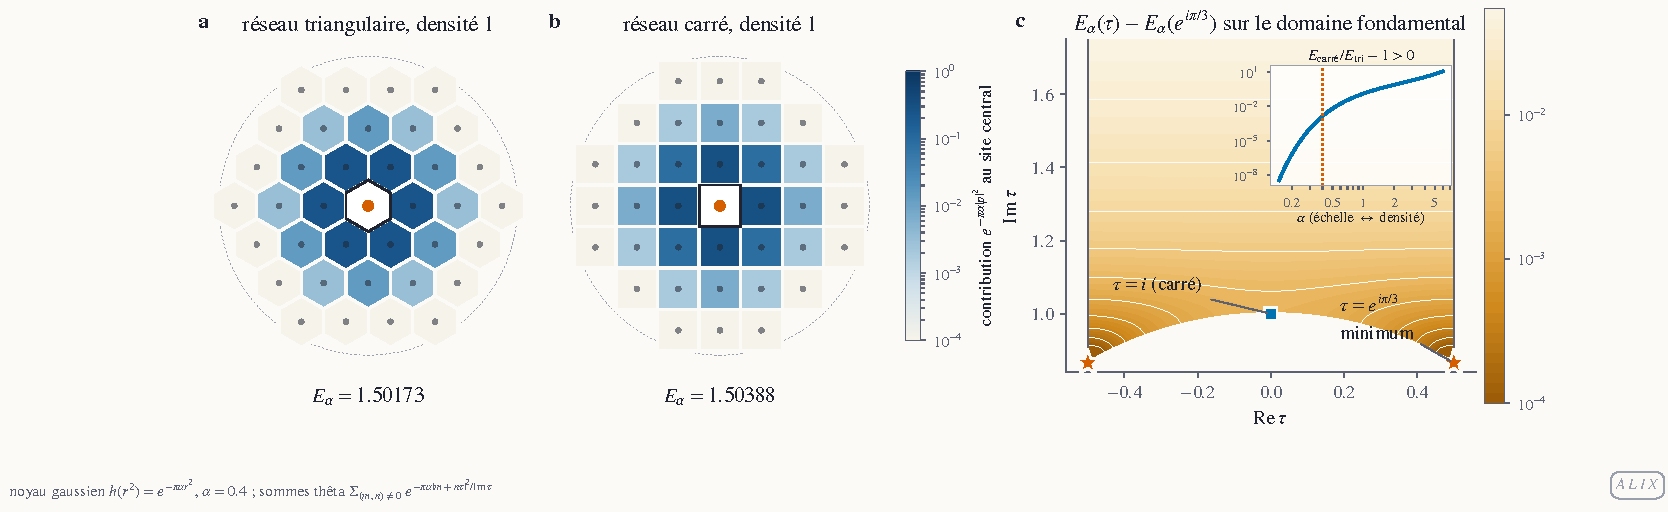
\includegraphics[width=\textwidth]{egg_ALIX.pdf}
\caption{\lean{ALIX}, \emph{A Lattice Is eXtremal}. The theorem \tierA{} (conditional on the upstream theorem
\lean{universal_energy_minimum} of openai/math, AI-generated and not peer reviewed) states that at every density
$\rho>0$ the triangular lattice minimizes the energy of every admissible potential, among all locally finite
configurations of density~$\rho$. The image \tierX{} takes the Gaussian kernel $e^{-\pi\alpha r^2}$, $\alpha=0.4$,
at density~1, and compares \emph{lattices} only. (a)~and~(b): Voronoi cells coloured by the contribution
$e^{-\pi\alpha|p|^2}$ of each site~$p$ to the energy of the central site; $E_\alpha=1.50173$ (triangular)
versus $1.50388$ (square). (c)~The difference $E_\alpha(\tau)-E_\alpha(e^{i\pi/3})$ over the fundamental domain of
lattice shapes, computed by theta sums; the grid minimum (at the equivalent point $-\tfrac12+i\tfrac{\sqrt3}2$, to within one grid step) and five
Nelder--Mead minimizations (to within $10^{-7}$) land back on $\tau=e^{i\pi/3}$. Inset: $E_{\text{square}}/E_{\text{tri}}-1>0$ for
$\alpha\in[0.15, 6]$, that is, for a whole range of densities.}
\label{fig:egg:ALIX}
\end{figure}

\begin{figure}[htbp]
\centering
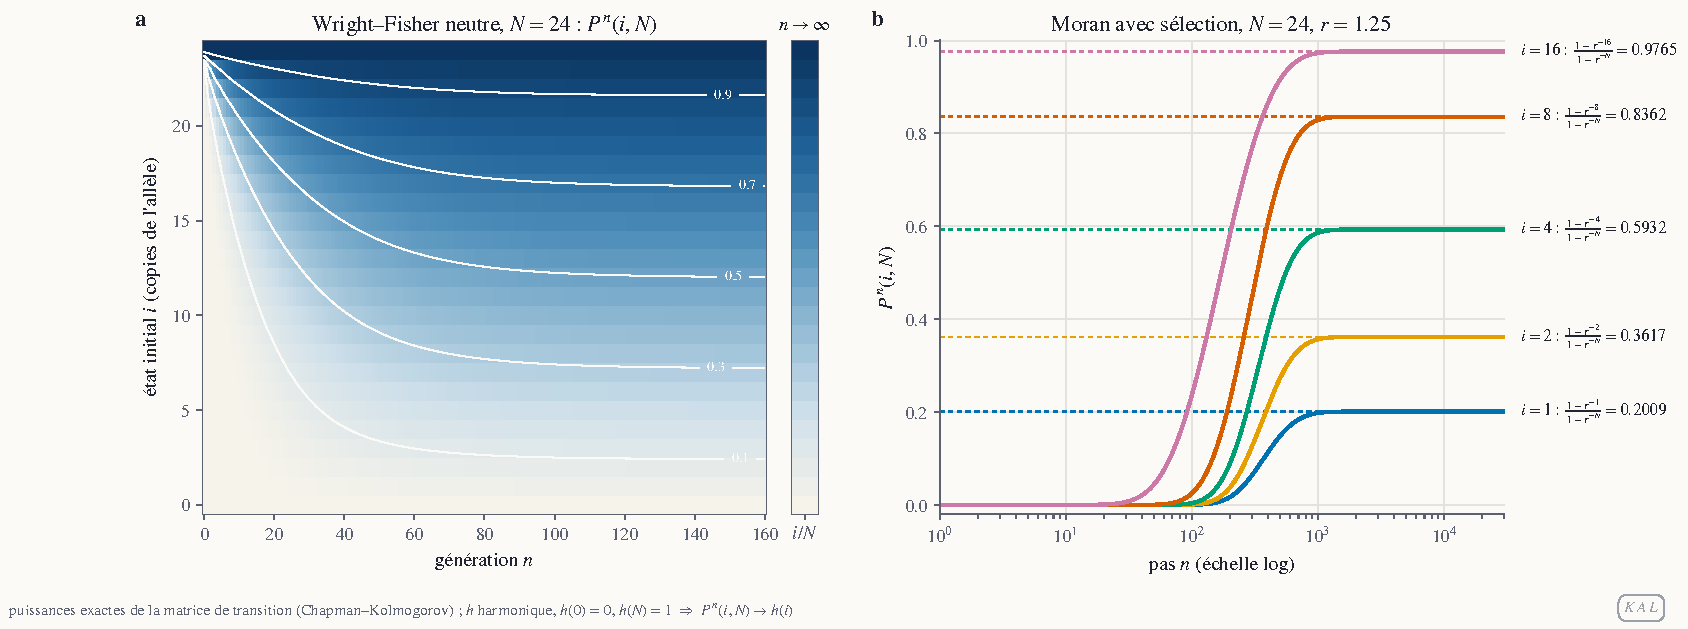
\includegraphics[width=\textwidth]{egg_KAL.pdf}
\caption{\lean{KAL}, \emph{Kolmogorov Absorption Limit}. The theorem \tierA{}: for a chain on
$\{0,\dots,N\}$ with absorbing boundaries, if $h$ is harmonic at the interior states, $h(0)=0$, $h(N)=1$, and the
one-step variance of $h$ is strictly positive, then $P^n(i,N)\to h(i)$ and $P^n(i,0)\to 1-h(i)$. Images
\tierX{}, by exact powers of the transition matrix. (a)~Neutral Wright--Fisher, $N=24$: $P^n(i,N)$
converges to $h(i)=i/N$ (right-hand band); maximal deviation at $n=4096$: $6\cdot10^{-16}$. (b)~Moran with
selection, $N=24$, $r=1.25$: $P^n(i,N)$ tends to $(1-r^{-i})/(1-r^{-N})$ (dotted), deviation
$7\cdot10^{-15}$ at $n=2^{22}$. The harmonicity of both functions $h$ is checked in exact rationals (for Wright--Fisher, at $N=8$).}
\label{fig:egg:KAL}
\end{figure}

\begin{figure}[htbp]
\centering
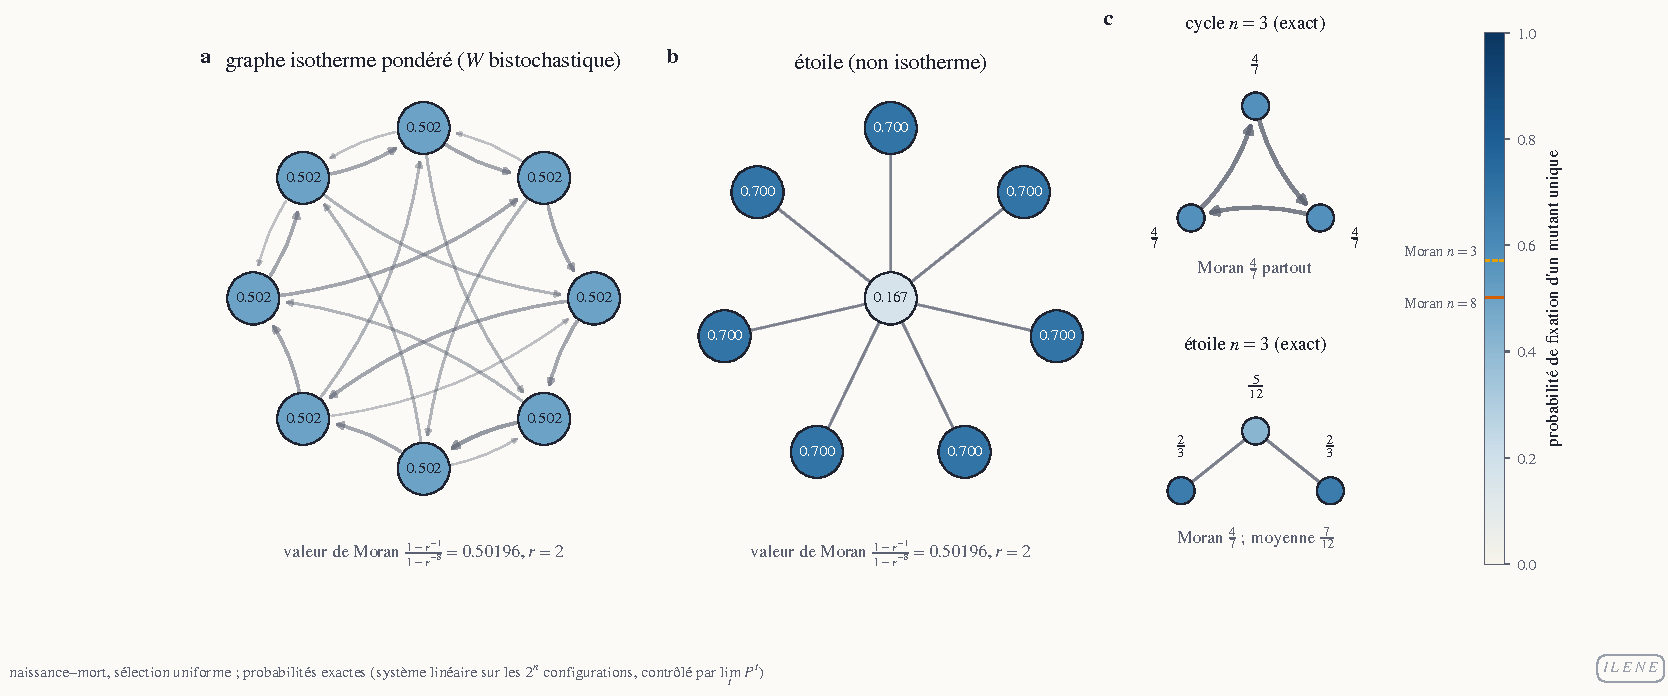
\includegraphics[width=\textwidth]{egg_ILENE.pdf}
\caption{\lean{ILENE}, \emph{Isothermal Law: Every Node Equivalent}. The theorem \tierA{}: on a strongly connected
isothermal graph ($W$ doubly stochastic), under birth--death with uniform selection, a single mutant of
fitness $r\neq1$ fixes with probability $(1-r^{-1})/(1-r^{-n})$, whatever its starting vertex. Images
\tierX{}, $r=2$, probabilities obtained by solving the linear system on the $2^n$ configurations (in floating
point for $n=8$, in rationals for $n=3$), and
checked against the limit of $P^t$. (a)~Weighted graph with $n=8$ vertices, $W=\frac12\Pi_1+\frac13\Pi_2+\frac16\Pi_3$
(three fixed-point-free permutations): all eight vertices give the Moran value $0.50196$ to within $2\cdot10^{-15}$.
(b)~The star with 7 leaves is not isothermal and lies outside the hypotheses: centre $0.167$, leaves $0.700$.
(c)~Rational computation for $n=3$: the 3-cycle gives $\frac47$ everywhere; the star gives $\frac5{12}$ at the centre and
$\frac23$ at the leaves, with mean $\frac7{12}\neq\frac47$.}
\label{fig:egg:ILENE}
\end{figure}

\begin{figure}[htbp]
\centering
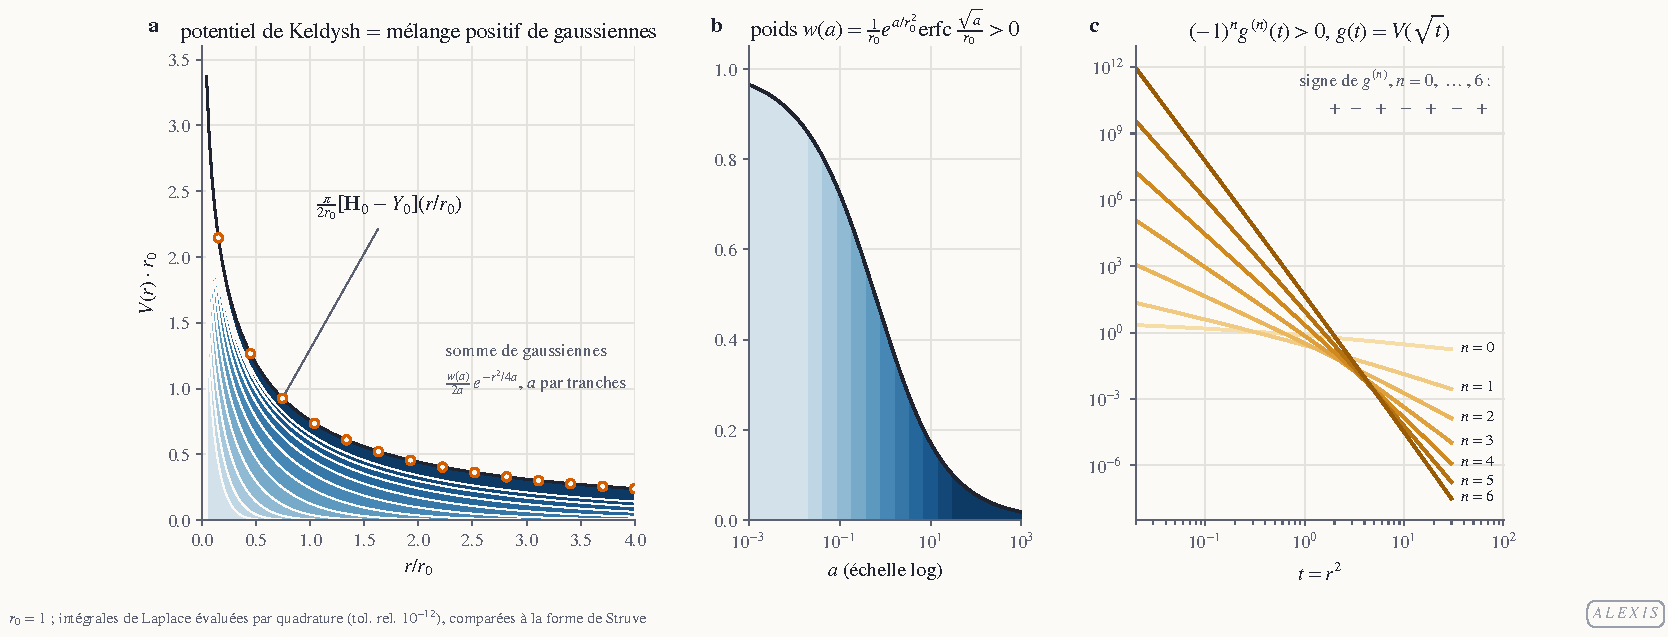
\includegraphics[width=\textwidth]{egg_ALEXIS.pdf}
\caption{\lean{ALEXIS}, \emph{Averaged Laplace EXponentials Inherit Signs}. The theorem \tierA{}: a positive
mixture of exponentials $t\mapsto\int e^{-t\,k(x)}m(x)\,d\mu(x)$ is an admissible potential, of class
$C^\infty$ on $(0,+\infty)$, positive, with $(-1)^n g^{(n)}\ge0$. The image \tierX{} shows one instance, the
Rytova--Keldysh potential ($r_0=1$), written as a Gaussian mixture
$V(r)=\int_0^\infty \frac{w(a)}{2a}\,e^{-r^2/4a}\,da$ with weight $w(a)=\frac1{r_0}e^{a/r_0^2}\operatorname{erfc}
(\sqrt a/r_0)>0$. (a)~The contributions of twelve slices in $a$, stacked, reproduce the Struve form
$\frac{\pi}{2r_0}[\mathbf H_0-Y_0](r/r_0)$ (dots) to within $3\cdot10^{-13}$ in relative terms; the identification
with the Struve form is a human proof, not machine-checked \tierC{}. (b)~The weight $w$, coloured by slice.
(c)~$(-1)^n g^{(n)}(t)$, $g(t)=V(\sqrt t)$, for $n=0,\dots,6$: all curves are positive, so the
derivatives $g^{(n)}$ alternate in sign; $n=1$ is cross-checked by finite differences of the Struve form.}
\label{fig:egg:ALEXIS}
\end{figure}

\begin{figure}[htbp]
\centering
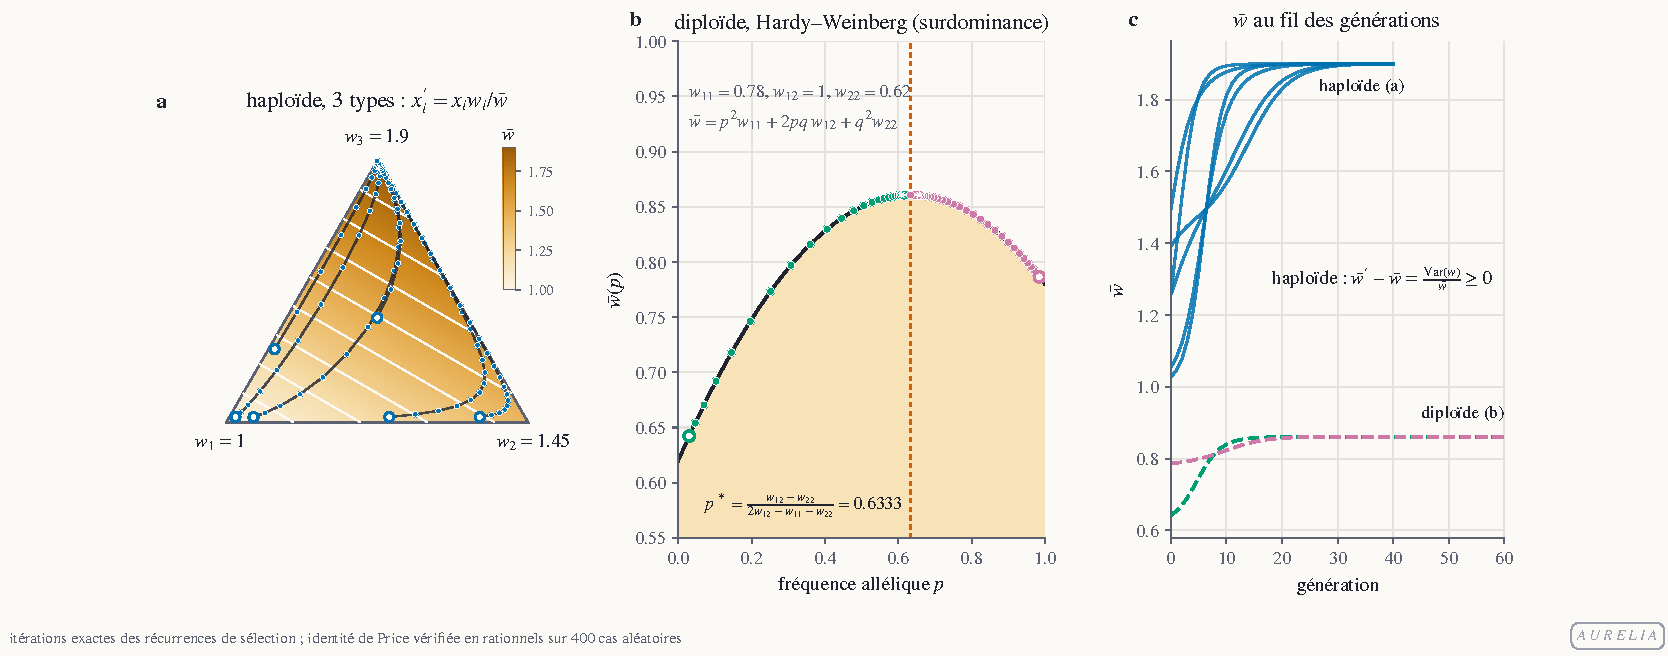
\includegraphics[width=\textwidth]{egg_AURELIA.pdf}
\caption{\lean{AURELIA}, \emph{Average Under Replication: Evolution Lifts It, Always}. The theorem \tierA{}:
under haploid selection with constant fitnesses and no transmission bias, mean fitness does not decrease,
$\bar w\le\bar w'$; this is a special case of Fisher's fundamental theorem, derived from the Price equation.
Images \tierX{}. (a)~Three types, $w=(1, 1.45, 1.9)$: on the simplex coloured by $\bar w$, six trajectories
of $x_i'=x_iw_i/\bar w$ climb towards the best type. (b)~Diploid case under Hardy--Weinberg, with overdominance
($w_{11}=0.78$, $w_{12}=1$, $w_{22}=0.62$): both trajectories climb $\bar w(p)$ up to
$p^*=0.6333$. This panel falls under the diploid theorem \lean{wbar_increment} of Chapter~4 (H12) \tierA{}, not under
\lean{AURELIA}. (c)~$\bar w$ over the generations, never decreasing. The identity
$\bar w'-\bar w=\mathrm{Var}(w)/\bar w$ is checked in exact rationals on 400 random cases; negative
control: with a mutation bias from the best type towards the worst, $\bar w$ drops by $0.35$.}
\label{fig:egg:AURELIA}
\end{figure}
).
% Figures produced by code/easter_egg_images.py (matplotlib/numpy/scipy); every plotted quantity is computed
% from its formula. The numerical self-checks (positive and negative controls) are recorded in
% results/textbook_formalisation_2026/easter_eggs_selfcheck.json; a failing check aborts the script.
\section*{The five images}
\addcontentsline{toc}{section}{The five images}

Each of the five short names of Section~\ref{ch5:acronymes} receives an image here. The tier of the theorem
(\tierA{}) refers to the re-exported Lean statement. The curves, colours and displayed values are numerical
computations \tierX{}: they illustrate a special case of the statement, without proving or extending it.

\begin{figure}[htbp]
\centering
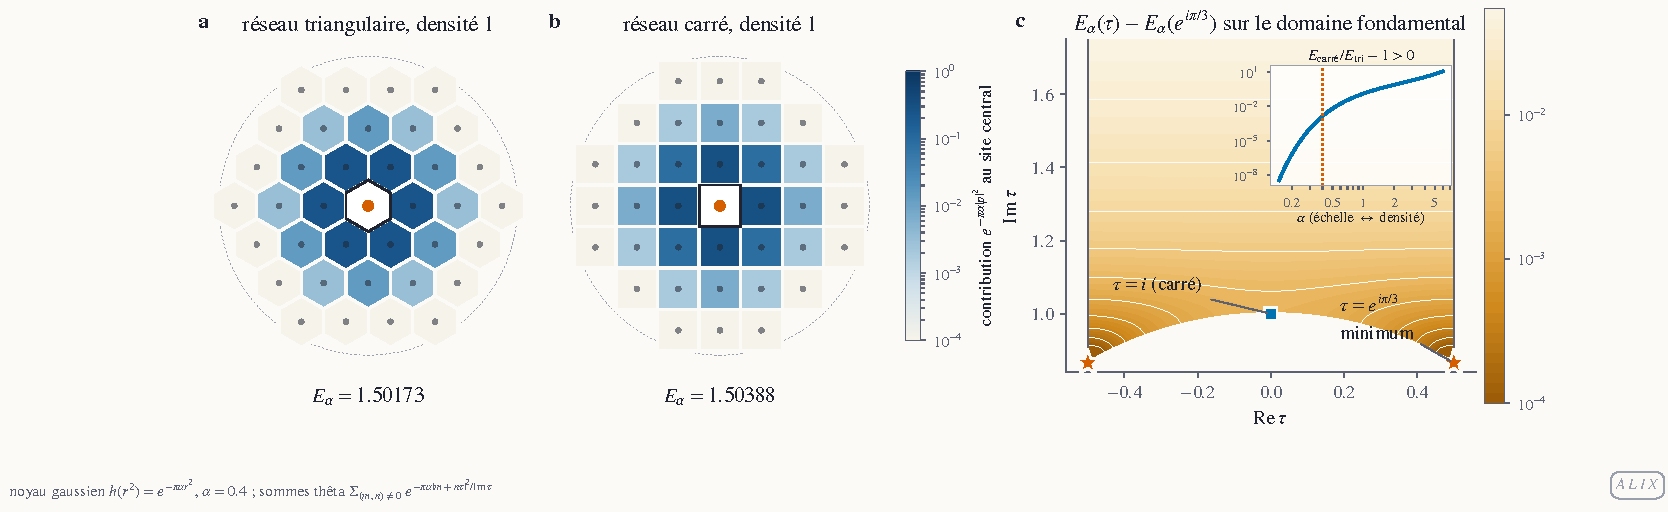
\includegraphics[width=\textwidth]{egg_ALIX.pdf}
\caption{\lean{ALIX}, \emph{A Lattice Is eXtremal}. The theorem \tierA{} (conditional on the upstream theorem
\lean{universal_energy_minimum} of openai/math, AI-generated and not peer reviewed) states that at every density
$\rho>0$ the triangular lattice minimizes the energy of every admissible potential, among all locally finite
configurations of density~$\rho$. The image \tierX{} takes the Gaussian kernel $e^{-\pi\alpha r^2}$, $\alpha=0.4$,
at density~1, and compares \emph{lattices} only. (a)~and~(b): Voronoi cells coloured by the contribution
$e^{-\pi\alpha|p|^2}$ of each site~$p$ to the energy of the central site; $E_\alpha=1.50173$ (triangular)
versus $1.50388$ (square). (c)~The difference $E_\alpha(\tau)-E_\alpha(e^{i\pi/3})$ over the fundamental domain of
lattice shapes, computed by theta sums; the grid minimum (at the equivalent point $-\tfrac12+i\tfrac{\sqrt3}2$, to within one grid step) and five
Nelder--Mead minimizations (to within $10^{-7}$) land back on $\tau=e^{i\pi/3}$. Inset: $E_{\text{square}}/E_{\text{tri}}-1>0$ for
$\alpha\in[0.15, 6]$, that is, for a whole range of densities.}
\label{fig:egg:ALIX}
\end{figure}

\begin{figure}[htbp]
\centering
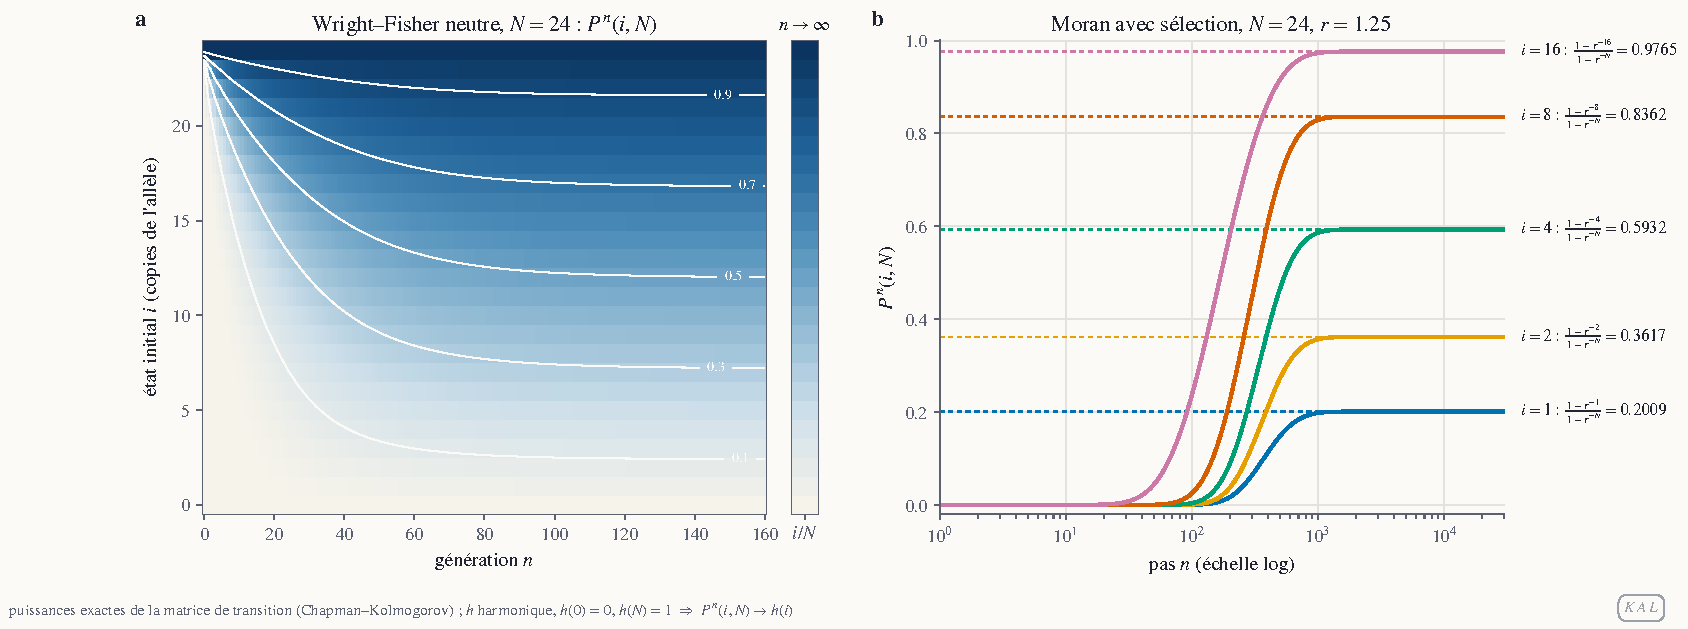
\includegraphics[width=\textwidth]{egg_KAL.pdf}
\caption{\lean{KAL}, \emph{Kolmogorov Absorption Limit}. The theorem \tierA{}: for a chain on
$\{0,\dots,N\}$ with absorbing boundaries, if $h$ is harmonic at the interior states, $h(0)=0$, $h(N)=1$, and the
one-step variance of $h$ is strictly positive, then $P^n(i,N)\to h(i)$ and $P^n(i,0)\to 1-h(i)$. Images
\tierX{}, by exact powers of the transition matrix. (a)~Neutral Wright--Fisher, $N=24$: $P^n(i,N)$
converges to $h(i)=i/N$ (right-hand band); maximal deviation at $n=4096$: $6\cdot10^{-16}$. (b)~Moran with
selection, $N=24$, $r=1.25$: $P^n(i,N)$ tends to $(1-r^{-i})/(1-r^{-N})$ (dotted), deviation
$7\cdot10^{-15}$ at $n=2^{22}$. The harmonicity of both functions $h$ is checked in exact rationals (for Wright--Fisher, at $N=8$).}
\label{fig:egg:KAL}
\end{figure}

\begin{figure}[htbp]
\centering
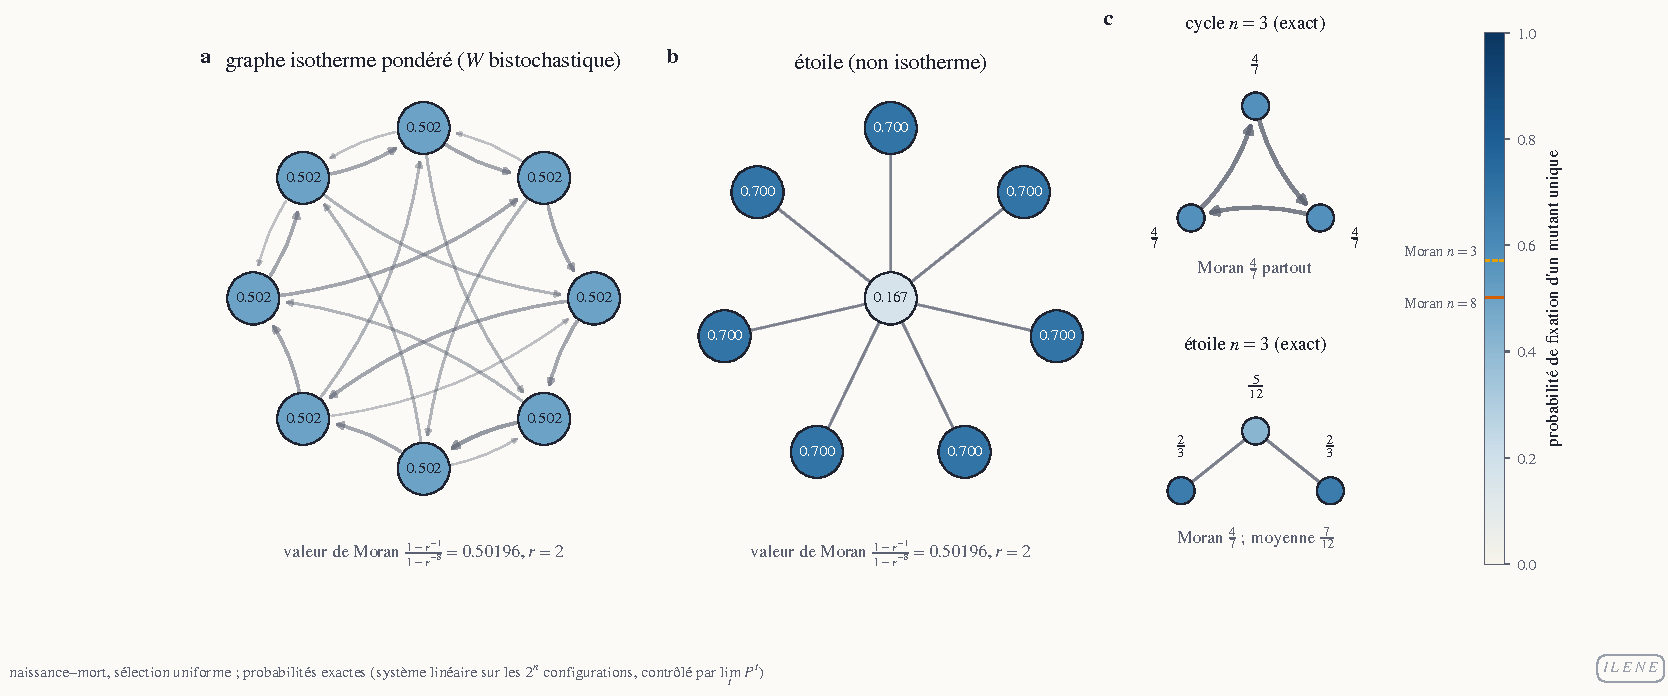
\includegraphics[width=\textwidth]{egg_ILENE.pdf}
\caption{\lean{ILENE}, \emph{Isothermal Law: Every Node Equivalent}. The theorem \tierA{}: on a strongly connected
isothermal graph ($W$ doubly stochastic), under birth--death with uniform selection, a single mutant of
fitness $r\neq1$ fixes with probability $(1-r^{-1})/(1-r^{-n})$, whatever its starting vertex. Images
\tierX{}, $r=2$, probabilities obtained by solving the linear system on the $2^n$ configurations (in floating
point for $n=8$, in rationals for $n=3$), and
checked against the limit of $P^t$. (a)~Weighted graph with $n=8$ vertices, $W=\frac12\Pi_1+\frac13\Pi_2+\frac16\Pi_3$
(three fixed-point-free permutations): all eight vertices give the Moran value $0.50196$ to within $2\cdot10^{-15}$.
(b)~The star with 7 leaves is not isothermal and lies outside the hypotheses: centre $0.167$, leaves $0.700$.
(c)~Rational computation for $n=3$: the 3-cycle gives $\frac47$ everywhere; the star gives $\frac5{12}$ at the centre and
$\frac23$ at the leaves, with mean $\frac7{12}\neq\frac47$.}
\label{fig:egg:ILENE}
\end{figure}

\begin{figure}[htbp]
\centering
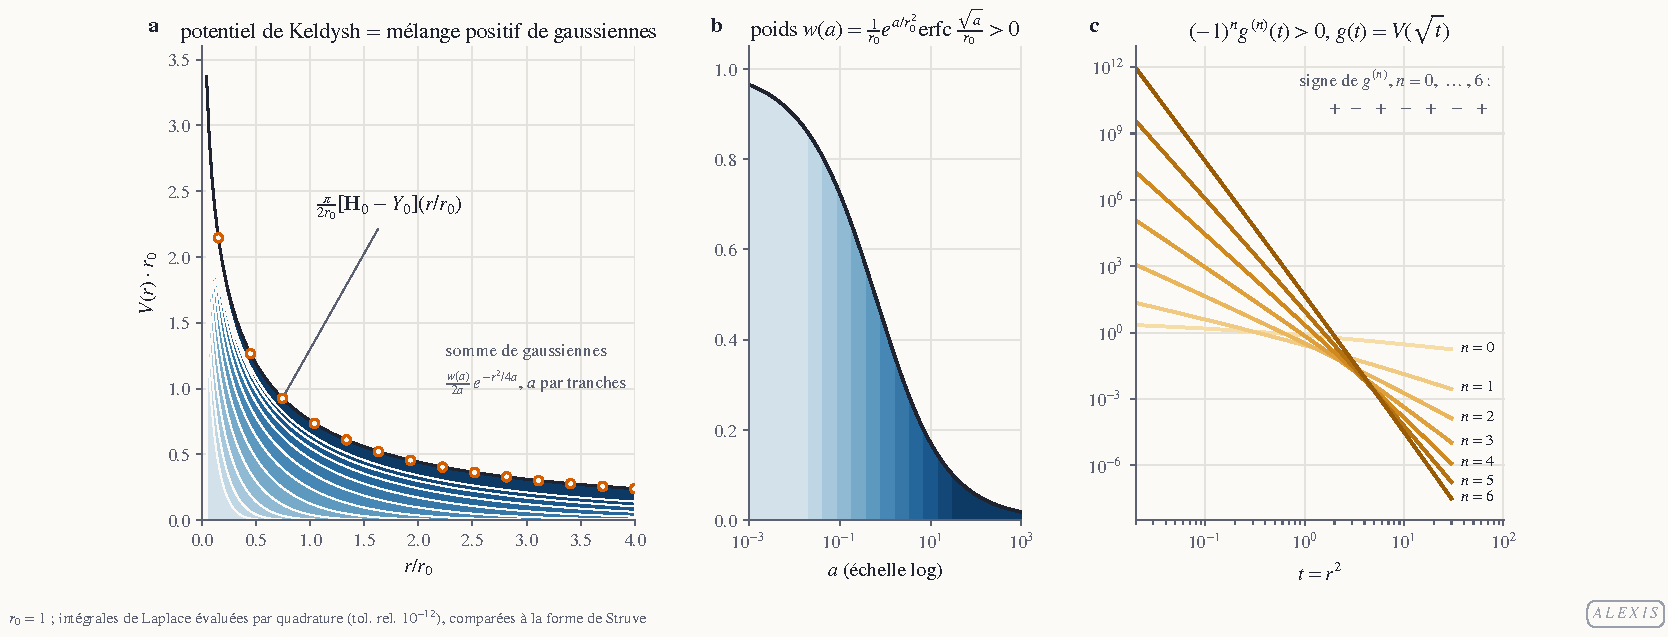
\includegraphics[width=\textwidth]{egg_ALEXIS.pdf}
\caption{\lean{ALEXIS}, \emph{Averaged Laplace EXponentials Inherit Signs}. The theorem \tierA{}: a positive
mixture of exponentials $t\mapsto\int e^{-t\,k(x)}m(x)\,d\mu(x)$ is an admissible potential, of class
$C^\infty$ on $(0,+\infty)$, positive, with $(-1)^n g^{(n)}\ge0$. The image \tierX{} shows one instance, the
Rytova--Keldysh potential ($r_0=1$), written as a Gaussian mixture
$V(r)=\int_0^\infty \frac{w(a)}{2a}\,e^{-r^2/4a}\,da$ with weight $w(a)=\frac1{r_0}e^{a/r_0^2}\operatorname{erfc}
(\sqrt a/r_0)>0$. (a)~The contributions of twelve slices in $a$, stacked, reproduce the Struve form
$\frac{\pi}{2r_0}[\mathbf H_0-Y_0](r/r_0)$ (dots) to within $3\cdot10^{-13}$ in relative terms; the identification
with the Struve form is a human proof, not machine-checked \tierC{}. (b)~The weight $w$, coloured by slice.
(c)~$(-1)^n g^{(n)}(t)$, $g(t)=V(\sqrt t)$, for $n=0,\dots,6$: all curves are positive, so the
derivatives $g^{(n)}$ alternate in sign; $n=1$ is cross-checked by finite differences of the Struve form.}
\label{fig:egg:ALEXIS}
\end{figure}

\begin{figure}[htbp]
\centering
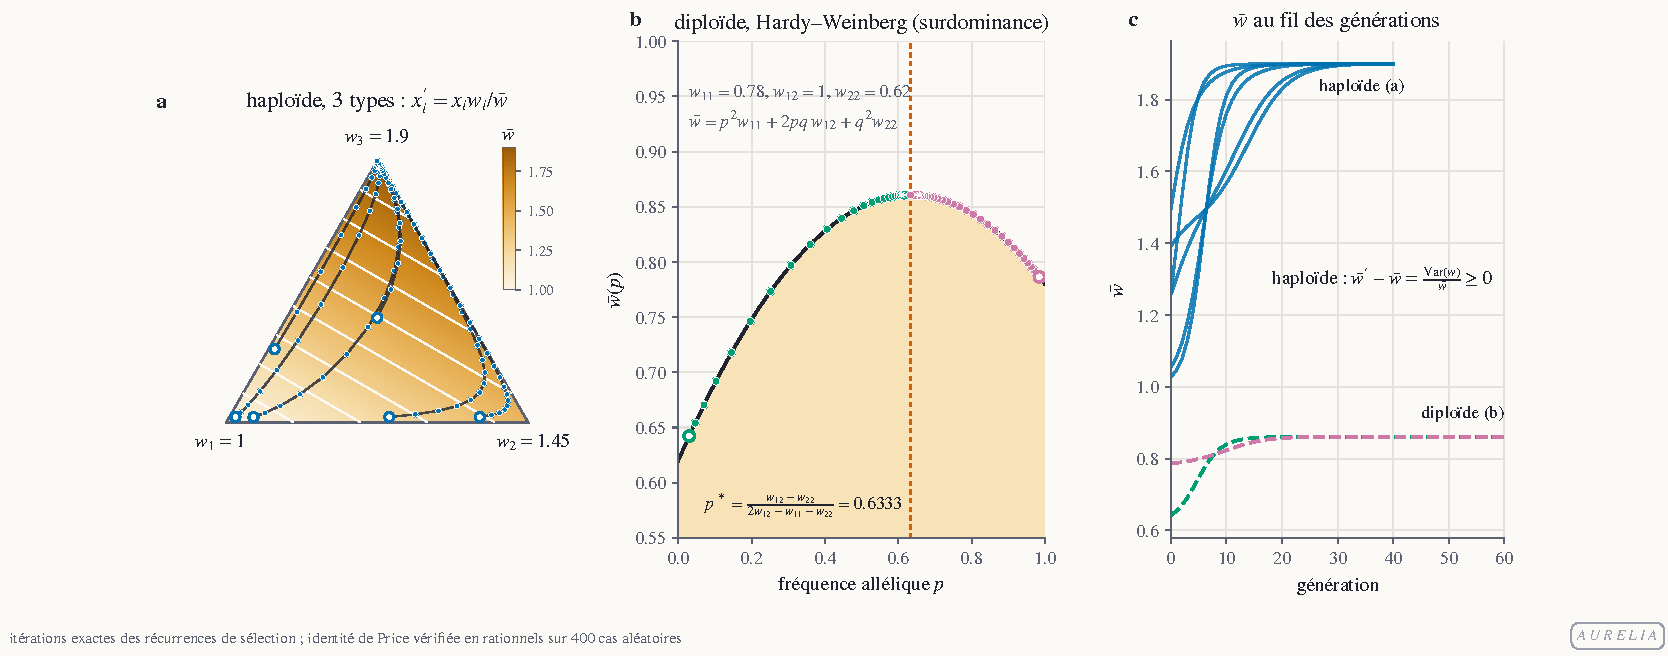
\includegraphics[width=\textwidth]{egg_AURELIA.pdf}
\caption{\lean{AURELIA}, \emph{Average Under Replication: Evolution Lifts It, Always}. The theorem \tierA{}:
under haploid selection with constant fitnesses and no transmission bias, mean fitness does not decrease,
$\bar w\le\bar w'$; this is a special case of Fisher's fundamental theorem, derived from the Price equation.
Images \tierX{}. (a)~Three types, $w=(1, 1.45, 1.9)$: on the simplex coloured by $\bar w$, six trajectories
of $x_i'=x_iw_i/\bar w$ climb towards the best type. (b)~Diploid case under Hardy--Weinberg, with overdominance
($w_{11}=0.78$, $w_{12}=1$, $w_{22}=0.62$): both trajectories climb $\bar w(p)$ up to
$p^*=0.6333$. This panel falls under the diploid theorem \lean{wbar_increment} of Chapter~4 (H12) \tierA{}, not under
\lean{AURELIA}. (c)~$\bar w$ over the generations, never decreasing. The identity
$\bar w'-\bar w=\mathrm{Var}(w)/\bar w$ is checked in exact rationals on 400 random cases; negative
control: with a mutation bias from the best type towards the worst, $\bar w$ drops by $0.35$.}
\label{fig:egg:AURELIA}
\end{figure}
).
% Figures produced by code/easter_egg_images.py (matplotlib/numpy/scipy); every plotted quantity is computed
% from its formula. The numerical self-checks (positive and negative controls) are recorded in
% results/textbook_formalisation_2026/easter_eggs_selfcheck.json; a failing check aborts the script.
\section*{The five images}
\addcontentsline{toc}{section}{The five images}

Each of the five short names of Section~\ref{ch5:acronymes} receives an image here. The tier of the theorem
(\tierA{}) refers to the re-exported Lean statement. The curves, colours and displayed values are numerical
computations \tierX{}: they illustrate a special case of the statement, without proving or extending it.

\begin{figure}[htbp]
\centering
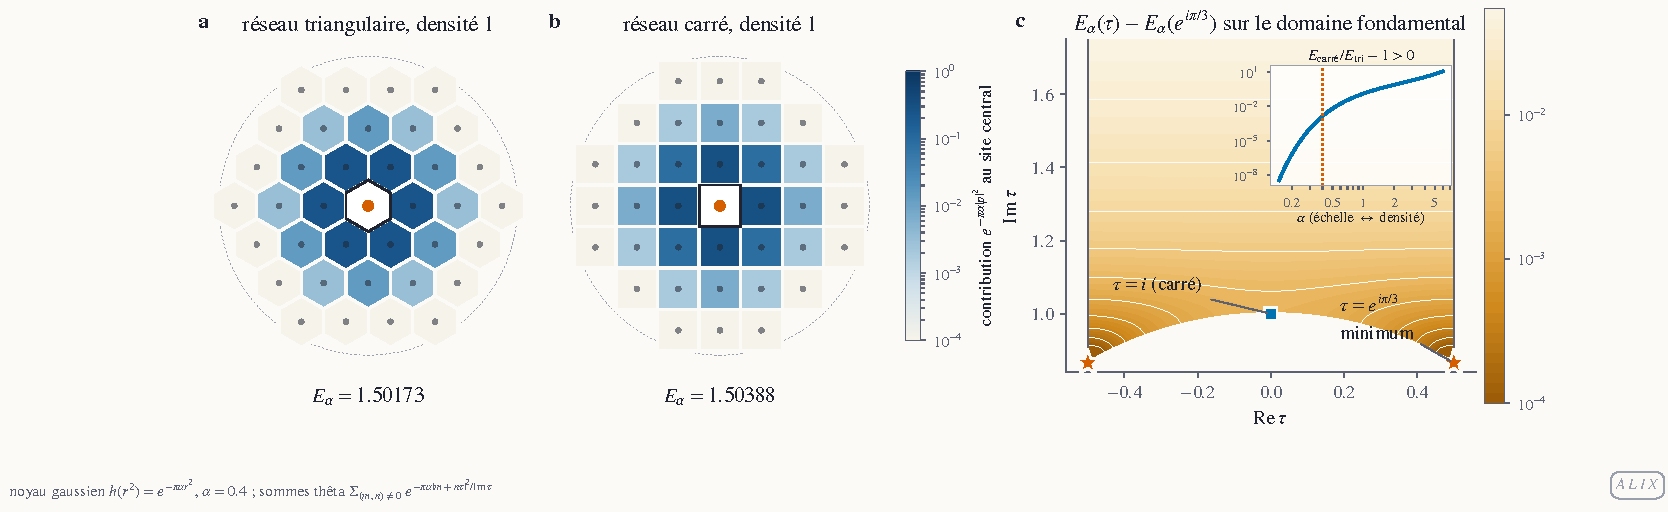
\includegraphics[width=\textwidth]{egg_ALIX.pdf}
\caption{\lean{ALIX}, \emph{A Lattice Is eXtremal}. The theorem \tierA{} (conditional on the upstream theorem
\lean{universal_energy_minimum} of openai/math, AI-generated and not peer reviewed) states that at every density
$\rho>0$ the triangular lattice minimizes the energy of every admissible potential, among all locally finite
configurations of density~$\rho$. The image \tierX{} takes the Gaussian kernel $e^{-\pi\alpha r^2}$, $\alpha=0.4$,
at density~1, and compares \emph{lattices} only. (a)~and~(b): Voronoi cells coloured by the contribution
$e^{-\pi\alpha|p|^2}$ of each site~$p$ to the energy of the central site; $E_\alpha=1.50173$ (triangular)
versus $1.50388$ (square). (c)~The difference $E_\alpha(\tau)-E_\alpha(e^{i\pi/3})$ over the fundamental domain of
lattice shapes, computed by theta sums; the grid minimum (at the equivalent point $-\tfrac12+i\tfrac{\sqrt3}2$, to within one grid step) and five
Nelder--Mead minimizations (to within $10^{-7}$) land back on $\tau=e^{i\pi/3}$. Inset: $E_{\text{square}}/E_{\text{tri}}-1>0$ for
$\alpha\in[0.15, 6]$, that is, for a whole range of densities.}
\label{fig:egg:ALIX}
\end{figure}

\begin{figure}[htbp]
\centering
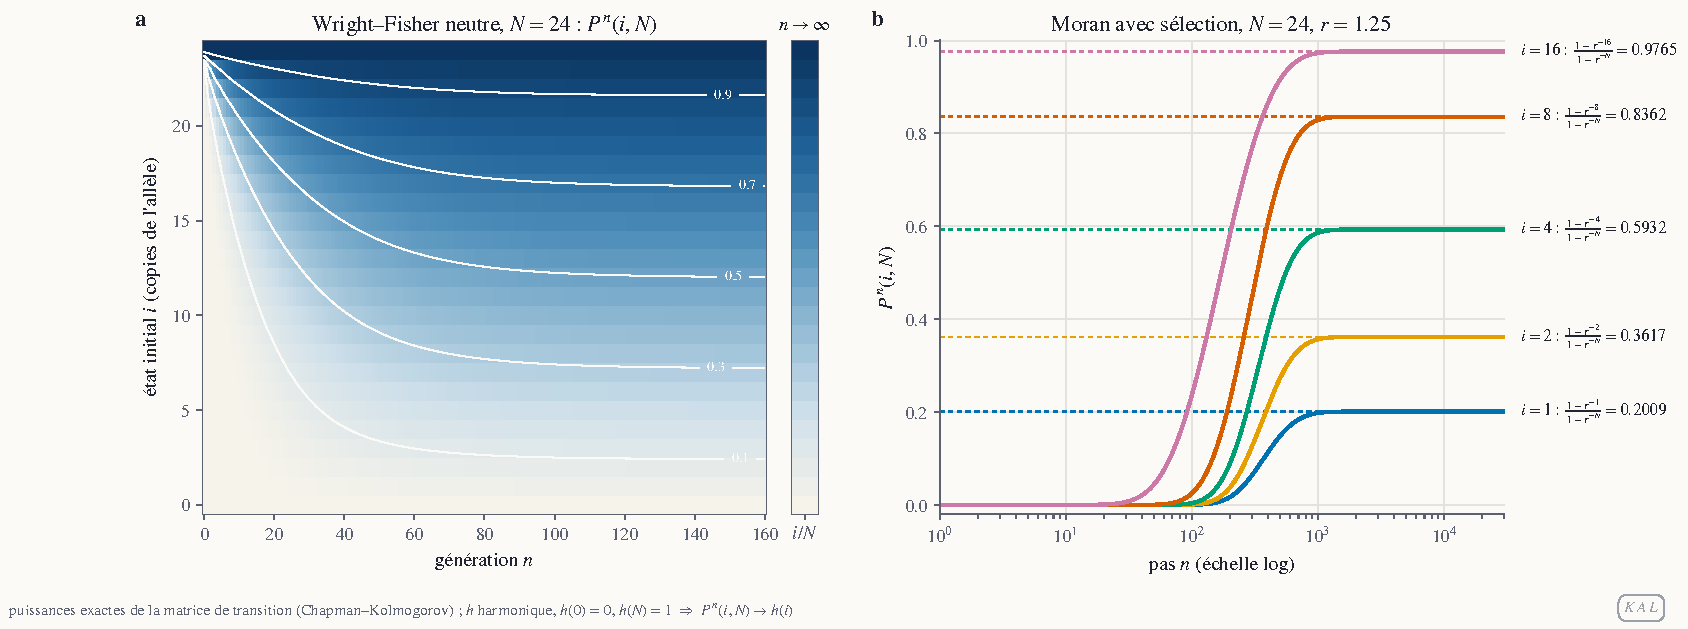
\includegraphics[width=\textwidth]{egg_KAL.pdf}
\caption{\lean{KAL}, \emph{Kolmogorov Absorption Limit}. The theorem \tierA{}: for a chain on
$\{0,\dots,N\}$ with absorbing boundaries, if $h$ is harmonic at the interior states, $h(0)=0$, $h(N)=1$, and the
one-step variance of $h$ is strictly positive, then $P^n(i,N)\to h(i)$ and $P^n(i,0)\to 1-h(i)$. Images
\tierX{}, by exact powers of the transition matrix. (a)~Neutral Wright--Fisher, $N=24$: $P^n(i,N)$
converges to $h(i)=i/N$ (right-hand band); maximal deviation at $n=4096$: $6\cdot10^{-16}$. (b)~Moran with
selection, $N=24$, $r=1.25$: $P^n(i,N)$ tends to $(1-r^{-i})/(1-r^{-N})$ (dotted), deviation
$7\cdot10^{-15}$ at $n=2^{22}$. The harmonicity of both functions $h$ is checked in exact rationals (for Wright--Fisher, at $N=8$).}
\label{fig:egg:KAL}
\end{figure}

\begin{figure}[htbp]
\centering
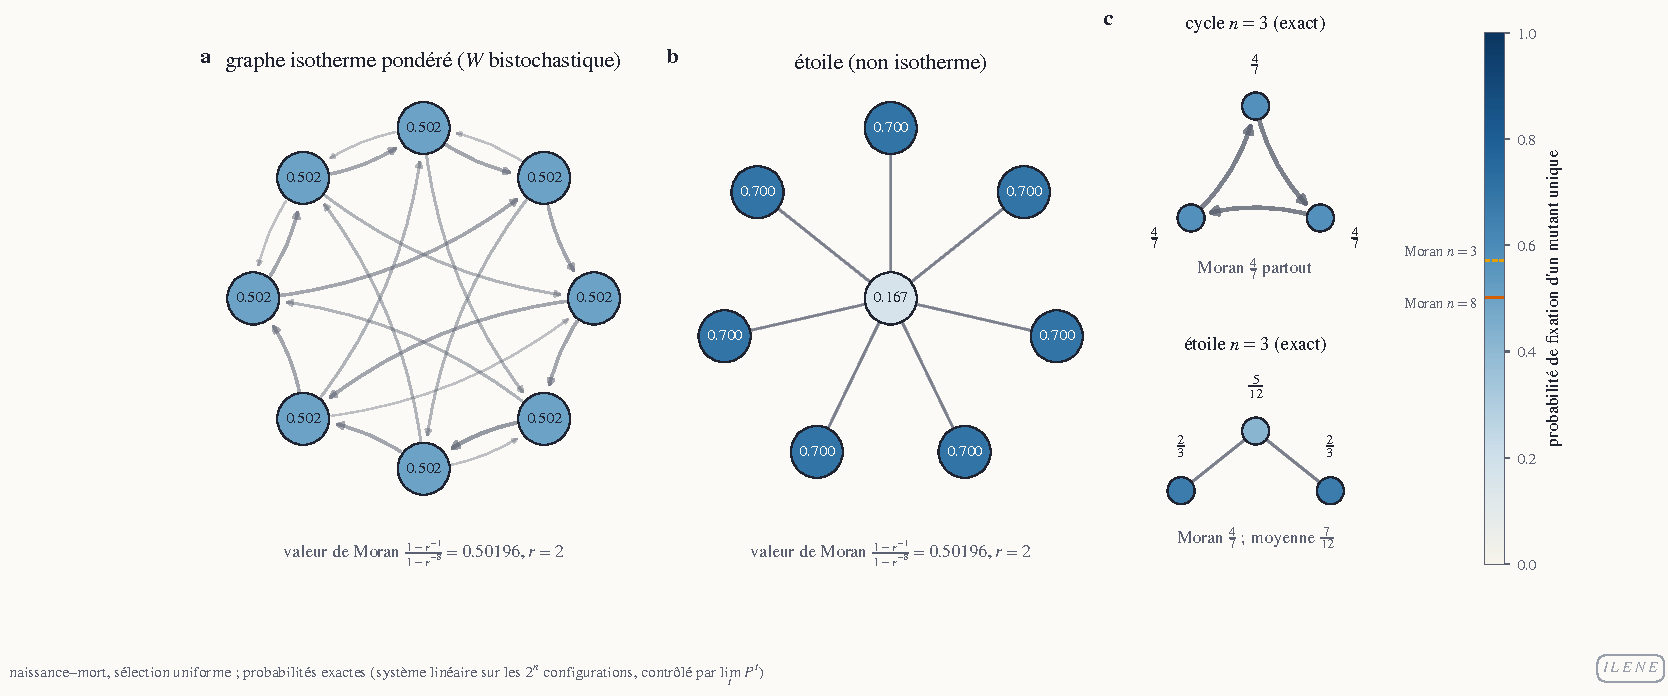
\includegraphics[width=\textwidth]{egg_ILENE.pdf}
\caption{\lean{ILENE}, \emph{Isothermal Law: Every Node Equivalent}. The theorem \tierA{}: on a strongly connected
isothermal graph ($W$ doubly stochastic), under birth--death with uniform selection, a single mutant of
fitness $r\neq1$ fixes with probability $(1-r^{-1})/(1-r^{-n})$, whatever its starting vertex. Images
\tierX{}, $r=2$, probabilities obtained by solving the linear system on the $2^n$ configurations (in floating
point for $n=8$, in rationals for $n=3$), and
checked against the limit of $P^t$. (a)~Weighted graph with $n=8$ vertices, $W=\frac12\Pi_1+\frac13\Pi_2+\frac16\Pi_3$
(three fixed-point-free permutations): all eight vertices give the Moran value $0.50196$ to within $2\cdot10^{-15}$.
(b)~The star with 7 leaves is not isothermal and lies outside the hypotheses: centre $0.167$, leaves $0.700$.
(c)~Rational computation for $n=3$: the 3-cycle gives $\frac47$ everywhere; the star gives $\frac5{12}$ at the centre and
$\frac23$ at the leaves, with mean $\frac7{12}\neq\frac47$.}
\label{fig:egg:ILENE}
\end{figure}

\begin{figure}[htbp]
\centering
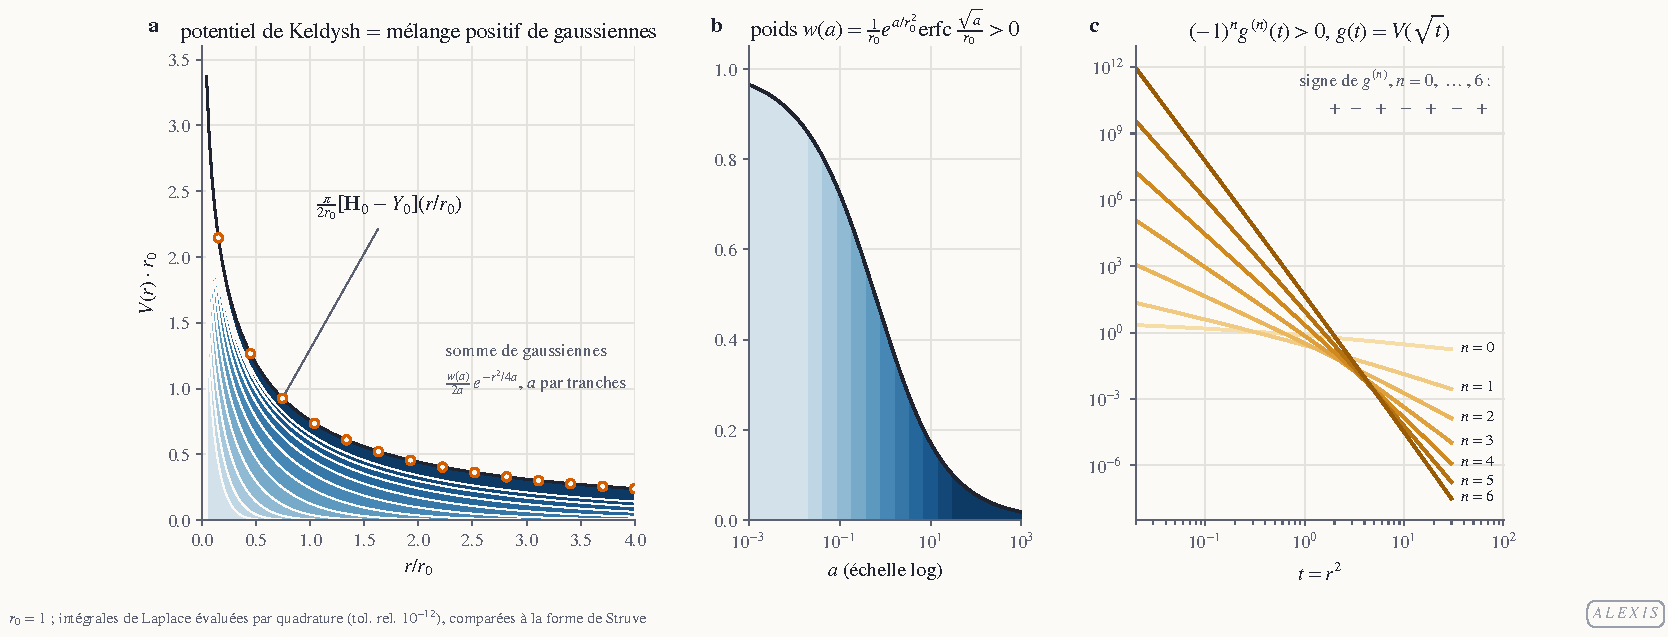
\includegraphics[width=\textwidth]{egg_ALEXIS.pdf}
\caption{\lean{ALEXIS}, \emph{Averaged Laplace EXponentials Inherit Signs}. The theorem \tierA{}: a positive
mixture of exponentials $t\mapsto\int e^{-t\,k(x)}m(x)\,d\mu(x)$ is an admissible potential, of class
$C^\infty$ on $(0,+\infty)$, positive, with $(-1)^n g^{(n)}\ge0$. The image \tierX{} shows one instance, the
Rytova--Keldysh potential ($r_0=1$), written as a Gaussian mixture
$V(r)=\int_0^\infty \frac{w(a)}{2a}\,e^{-r^2/4a}\,da$ with weight $w(a)=\frac1{r_0}e^{a/r_0^2}\operatorname{erfc}
(\sqrt a/r_0)>0$. (a)~The contributions of twelve slices in $a$, stacked, reproduce the Struve form
$\frac{\pi}{2r_0}[\mathbf H_0-Y_0](r/r_0)$ (dots) to within $3\cdot10^{-13}$ in relative terms; the identification
with the Struve form is a human proof, not machine-checked \tierC{}. (b)~The weight $w$, coloured by slice.
(c)~$(-1)^n g^{(n)}(t)$, $g(t)=V(\sqrt t)$, for $n=0,\dots,6$: all curves are positive, so the
derivatives $g^{(n)}$ alternate in sign; $n=1$ is cross-checked by finite differences of the Struve form.}
\label{fig:egg:ALEXIS}
\end{figure}

\begin{figure}[htbp]
\centering
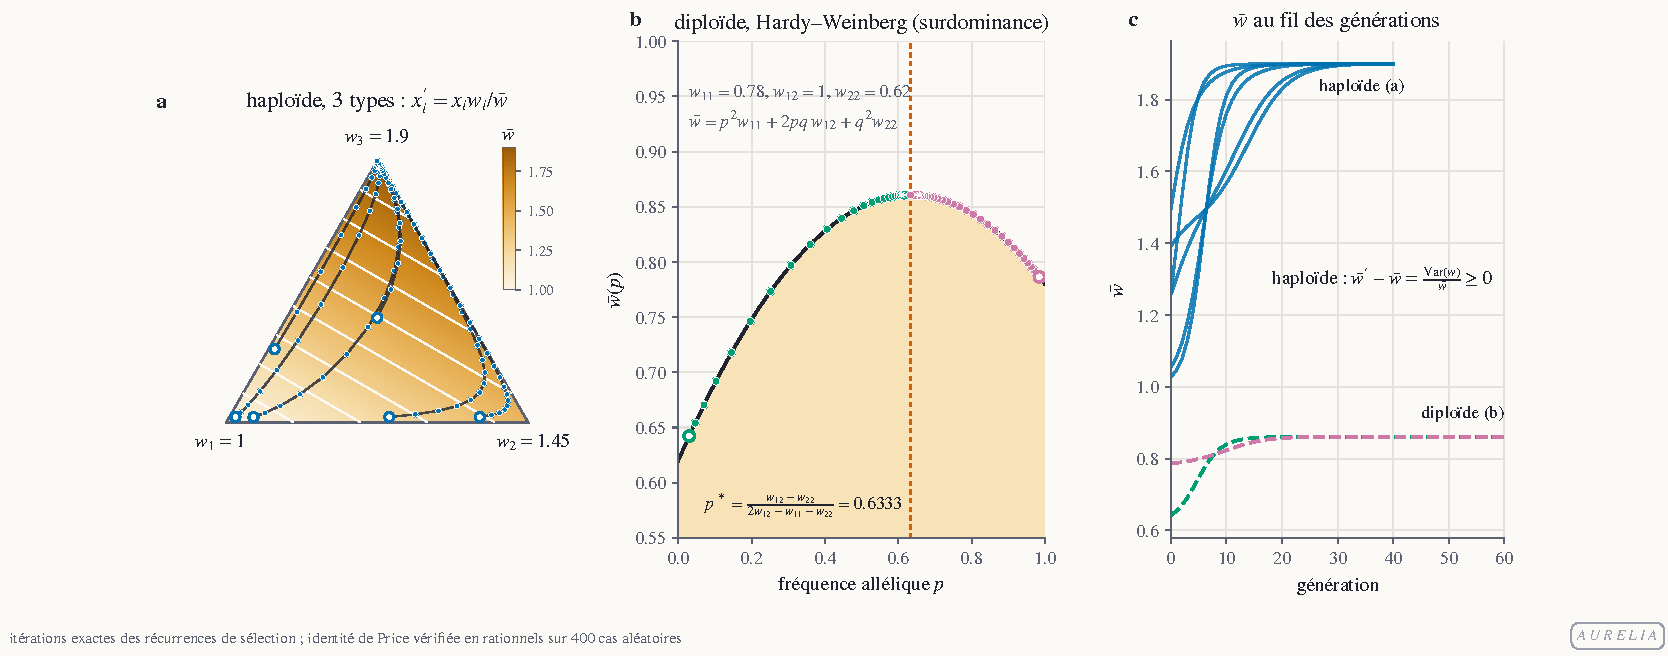
\includegraphics[width=\textwidth]{egg_AURELIA.pdf}
\caption{\lean{AURELIA}, \emph{Average Under Replication: Evolution Lifts It, Always}. The theorem \tierA{}:
under haploid selection with constant fitnesses and no transmission bias, mean fitness does not decrease,
$\bar w\le\bar w'$; this is a special case of Fisher's fundamental theorem, derived from the Price equation.
Images \tierX{}. (a)~Three types, $w=(1, 1.45, 1.9)$: on the simplex coloured by $\bar w$, six trajectories
of $x_i'=x_iw_i/\bar w$ climb towards the best type. (b)~Diploid case under Hardy--Weinberg, with overdominance
($w_{11}=0.78$, $w_{12}=1$, $w_{22}=0.62$): both trajectories climb $\bar w(p)$ up to
$p^*=0.6333$. This panel falls under the diploid theorem \lean{wbar_increment} of Chapter~4 (H12) \tierA{}, not under
\lean{AURELIA}. (c)~$\bar w$ over the generations, never decreasing. The identity
$\bar w'-\bar w=\mathrm{Var}(w)/\bar w$ is checked in exact rationals on 400 random cases; negative
control: with a mutation bias from the best type towards the worst, $\bar w$ drops by $0.35$.}
\label{fig:egg:AURELIA}
\end{figure}

\appendix
% Appendix A -- Analysis background. Include after \appendix via % Appendix A -- Analysis background. Include after \appendix via % Appendix A -- Analysis background. Include after \appendix via \input{appA_analyse.tex}.
% Labels prefixed appA: ; bibliography keys prefixed app: (refs_app.tex).
\chapter{Analysis background}\label{appA:chap}

This appendix collects the analytical tools that the chapters use without always re-proving them:
\begin{itemize}
\item interchanging a limit with an integral or a series (§\ref{appA:sec:param});
\item the Fourier and Laplace transforms (§\ref{appA:sec:fourier});
\item the Poisson summation formula, in the general case (§\ref{appA:sec:poisson});
\item the special functions that occur: $\Gamma$, $\operatorname{erfc}$, $J_0$, $K_0$, $Y_0$ and the Struve
function $\mathbf H_0$ (§\ref{appA:sec:speciales});
\item lattices in the plane and the fundamental domain of $SL_2(\Z)$ (§\ref{appA:sec:sl2}).
\end{itemize}
The level is that of a second-year undergraduate analysis course. The integral is Lebesgue's, but it suffices to be
able to apply the dominated convergence theorem and term-by-term integration of series, both recalled below.

\begin{warnbox}[: tiers of the statements in this appendix]
The proofs written here are human proofs \tierC{}: none of them is checked by Lean in this book.
The statements taken as given (dominated convergence, Fejér's theorem, properties of the Bessel and Struve functions
taken from the DLMF~\cite{app:dlmf}) are \tierL. The pinned Mathlib contains formal versions of several of them:
dominated convergence (\lean{MeasureTheory.tendsto_integral_of_dominated_convergence}, file
\texttt{MeasureTheory/Integral/DominatedConvergence.lean}) and the Poisson summation formula (files
\texttt{Analysis/Fourier/PoissonSummation.lean} and \texttt{Analysis/SpecialFunctions/Gaussian/PoissonSummation.lean}).
We have only checked that these files exist; we have neither compared their statements with those of this appendix,
nor connected those statements to the proofs below.
\end{warnbox}

%=====================================================================================================================
\section{Series and integrals depending on a parameter}\label{appA:sec:param}

\subsection{The dominated convergence theorem}

\begin{theorem}[Dominated convergence \tierL]\label{appA:thm:cvd}
Let $I$ be an interval of $\R$ and $(f_n)$ a sequence of piecewise continuous functions on $I$. Assume that:
\begin{enumerate}
\item $(f_n)$ converges pointwise on $I$ to a piecewise continuous function $f$;
\item there exists $\varphi:I\to\R_+$, integrable on $I$, such that $|f_n(x)|\le\varphi(x)$ for all $n$ and all $x$
(domination hypothesis).
\end{enumerate}
Then the $f_n$ and $f$ are integrable on $I$, and $\int_If_n\to\int_If$.
\end{theorem}

The essential point is that the dominating function $\varphi$ does not depend on $n$. Without it, the conclusion can
fail: $f_n=n\,\mathbf 1_{(0,1/n]}$ tends pointwise to $0$ on $(0,1]$, whereas $\int f_n=1$ for all $n$.

\begin{uniremark}\tierL{} The general form of Lebesgue's theorem holds on any measure space $(\Omega,\mathcal F,\mu)$:
if the $f_n$ are measurable, $f_n\to f$ $\mu$-almost everywhere, and $|f_n|\le g$ $\mu$-a.e.\ for every $n$ with
$g\in L^1(\mu)$, then $f\in L^1(\mu)$ and $\int|f_n-f|\,d\mu\to0$, hence $\int f_n\,d\mu\to\int f\,d\mu$. No continuity
is needed; the piecewise-continuous version above is the special case of Lebesgue measure on an interval. The
probabilistic form (expectations of a.s.\ convergent, dominated random variables) is the case $\mu(\Omega)=1$
\cite{app:williams}.
\end{uniremark}

\begin{theorem}[Interchanging series and integral \tierL]\label{appA:thm:serieint}
Let $(u_n)$ be a sequence of integrable functions on $I$ such that $\sum_n u_n$ converges pointwise to a piecewise
continuous function and $\sum_n\int_I|u_n|<\infty$. Then $\sum_nu_n$ is integrable and
$\int_I\sum_nu_n=\sum_n\int_Iu_n$.
\end{theorem}

\subsection{Continuity and differentiation under the integral sign}

\begin{theorem}[Continuity under the integral sign]\label{appA:thm:cont}
Let $A$ be a subset of $\R^p$ and $f:A\times I\to\mathbb{C}$ such that $f(\cdot,x)$ is continuous for every $x$, $f(a,\cdot)$
is piecewise continuous for every $a$, and $|f(a,x)|\le\varphi(x)$ with $\varphi$ integrable. Then
$F(a)=\int_If(a,x)\,dx$ is continuous on $A$.
\end{theorem}

\begin{humanproof}
Let $a_n\to a$ in $A$. The functions $x\mapsto f(a_n,x)$ converge pointwise to $f(a,\cdot)$ and are dominated by
$\varphi$. Theorem~\ref{appA:thm:cvd} gives $F(a_n)\to F(a)$, and the sequential characterisation of continuity
concludes.
\end{humanproof}

\begin{theorem}[Differentiation under the integral sign]\label{appA:thm:deriv}
Let $J$ be an interval and $f:J\times I\to\mathbb{C}$. Assume that $f(a,\cdot)$ is integrable for every $a\in J$, that
$\partial f/\partial a$ exists, is continuous in $a$ and piecewise continuous in $x$, and that there exists an integrable
$\psi$ with $|\partial_af(a,x)|\le\psi(x)$ for all $a,x$. Then $F(a)=\int_If(a,x)\,dx$ is of class $\mathcal C^1$ on $J$,
and $F'(a)=\int_I\partial_af(a,x)\,dx$.
\end{theorem}

\begin{humanproof}
Fix $a\in J$ and a sequence $h_n\to0$, $h_n\ne0$, with $a+h_n\in J$. Set
$g_n(x)=\bigl(f(a+h_n,x)-f(a,x)\bigr)/h_n$. By definition of the partial derivative, $g_n(x)\to\partial_af(a,x)$ for
every $x$. By the mean value inequality applied to $t\mapsto f(t,x)$ between $a$ and $a+h_n$,
$|g_n(x)|\le\sup_t|\partial_af(t,x)|\le\psi(x)$. Theorem~\ref{appA:thm:cvd} gives
$\bigl(F(a+h_n)-F(a)\bigr)/h_n=\int g_n\to\int\partial_af(a,x)\,dx$. The continuity of $F'$ follows from
Theorem~\ref{appA:thm:cont} applied to $\partial_af$.
\end{humanproof}

\begin{remark}[Local domination]
In practice it suffices that the domination hold on every compact interval $[\alpha,\beta]\subset J$: differentiability
is a local property. This is how the Laplace transforms below are handled, where the domination is uniform only
for $t\ge\alpha>0$.
\end{remark}

\begin{uniremark}\tierL{} In measure-theoretic form: let $(\Omega,\mathcal F,\mu)$ be a measure space, $J\subset\R$ an
open interval, and $f:J\times\Omega\to\mathbb C$ with $f(a,\cdot)\in L^1(\mu)$ for every $a\in J$. If, for $\mu$-a.e.\
$\omega$, the map $a\mapsto f(a,\omega)$ is differentiable on $J$ and $|\partial_af(a,\omega)|\le g(\omega)$ for all
$a\in J$, with $g\in L^1(\mu)$, then $F(a)=\int f(a,\omega)\,\mu(d\omega)$ is differentiable on
$J$ and $F'(a)=\int\partial_af(a,\omega)\,\mu(d\omega)$. The proof is the one above, with the general dominated
convergence theorem in place of Theorem~\ref{appA:thm:cvd} (standard).
\end{uniremark}

\begin{example}[Gaussian moments]\label{appA:ex:moments}
For $\alpha>0$, $G(\alpha)=\int_\R e^{-\pi\alpha x^2}dx=\alpha^{-1/2}$ (Gaussian integral). On $[\alpha_0,\infty)$ with
$\alpha_0>0$, $|\partial_\alpha e^{-\pi\alpha x^2}|=\pi x^2e^{-\pi\alpha x^2}\le\pi x^2e^{-\pi\alpha_0x^2}$, which is
integrable. Theorem~\ref{appA:thm:deriv} gives $\int\pi x^2e^{-\pi\alpha x^2}dx=-G'(\alpha)=\tfrac12\alpha^{-3/2}$.
Differentiating $m$ times, $\int(\pi x^2)^me^{-\pi\alpha x^2}dx=\frac{(2m)!}{4^mm!}\,\alpha^{-1/2-m}$
(Exercise~\ref{appA:exo:moments}). The same technique computes, in Chapter~1, the Fourier transform of a Gaussian
(Theorem~\ref{ch1:thm:poisson}, step~1).
\end{example}

\subsection{Series of functions}

\begin{proposition}[Normal convergence \tierL]\label{appA:prop:normale}
Let $(u_n)$ be continuous functions on a subset $A$ of $\R^d$ with $\sum_n\sup_A|u_n|<\infty$. Then
$\sum_nu_n$ converges uniformly on $A$ and its sum is continuous. If moreover the $u_n$ are $\mathcal C^1$ on an
open set and $\sum_n\sup|\nabla u_n|<\infty$, the sum is $\mathcal C^1$ and may be differentiated term by term.
\end{proposition}

\begin{example}[Theta series]
For a lattice $\Lambda$ in the plane and $\alpha\ge\alpha_0>0$, one has $|x|^2\ge c\,(m^2+n^2)$ for $x=mu+nv$
(Chapter~1), hence $e^{-\pi\alpha|x|^2}\le e^{-\pi\alpha_0c(m^2+n^2)}$, the general term of a convergent series. The
series $\Theta_\Lambda(\alpha)$ therefore converges normally on $[\alpha_0,\infty)$, and it is $\mathcal C^\infty$ in
$\alpha$ there: one may differentiate term by term as often as one likes. The lattice sums
$S(\alpha)=\sum|P|^2e^{-\pi\alpha|P|^2}$ of Chapter~3 are precisely $-\Theta_\Lambda'(\alpha)/\pi$.
\end{example}

%=====================================================================================================================
\section{Fourier and Laplace transforms}\label{appA:sec:fourier}

\subsection{The Fourier transform}

\begin{definition}
For integrable $f:\R^d\to\mathbb{C}$, the \emph{Fourier transform} of $f$ is
\[\hat f(\xi)=\int_{\R^d}f(x)\,e^{-2\pi i\,\xi\cdot x}\,dx,\qquad\xi\in\R^d .\]
\end{definition}
This is the convention of Chapter~1: the factor $2\pi$ sits in the exponent, and the inversion formula then has no
factor in front of the integral. Other books, especially in physics, write $\int f(x)e^{-ik\cdot x}dx$; one passes
from one to the other via $k=2\pi\xi$.

\begin{proposition}[Elementary properties]\label{appA:prop:fourierprop}
Let $f$ be integrable, $a\in\R^d$, $\lambda>0$ and $M$ an invertible matrix.
\begin{enumerate}
\item $\hat f$ is continuous and bounded by $\|f\|_1$.
\item Translation: $\widehat{f(\cdot-a)}(\xi)=e^{-2\pi i\,a\cdot\xi}\hat f(\xi)$.
\item Linear change of variables: $\widehat{f\circ M}(\xi)=|\det M|^{-1}\hat f(M^{-\mathsf T}\xi)$.
\item If $f$ is $\mathcal C^1$ and $f$ and $\partial_jf$ are integrable, then $\widehat{\partial_jf}(\xi)=2\pi
i\,\xi_j\hat f(\xi)$.
\end{enumerate}
\end{proposition}

\begin{humanproof}
(1) follows from Theorem~\ref{appA:thm:cont}, with $|f(x)e^{-2\pi i\xi\cdot x}|=|f(x)|$ (the version of Theorem~\ref{appA:thm:cont} for a function that is only integrable in $x$ has the same proof). (2) and (3) are the changes
of variables $y=x-a$ and $y=Mx$ (Jacobian $|\det M|$, and $\xi\cdot M^{-1}y=(M^{-\mathsf T}\xi)\cdot y$). (4) is an
integration by parts in $x_j$; the boundary term tends to $0$ along a sequence of bounds, because $f$ is integrable
and has an integrable derivative.
\end{humanproof}

\begin{example}[Gaussians]\label{appA:ex:gauss}
For $\alpha>0$, $\widehat{e^{-\pi\alpha|x|^2}}(\xi)=\alpha^{-d/2}e^{-\pi|\xi|^2/\alpha}$. The proof in dimension~1
(a differential equation for $\hat f$, obtained by differentiation under the integral sign) is step~1 of the proof
of Theorem~\ref{ch1:thm:poisson}; one passes to dimension $d$ by Fubini, since the exponential factorises. In
particular $e^{-\pi|x|^2}$ is its own Fourier transform. For a Gaussian with arbitrary covariance,
item~(3) of Proposition~\ref{appA:prop:fourierprop} gives the general formula.
\end{example}

\begin{theorem}[Inversion \tierL]\label{appA:thm:inversion}
If $f$ and $\hat f$ are integrable, then $f(x)=\int\hat f(\xi)e^{2\pi i\,\xi\cdot x}d\xi$ at every point where $f$ is
continuous.
\end{theorem}

\subsection{Radial functions in the plane and the Bessel function \texorpdfstring{$J_0$}{J0}}\label{appA:ssec:hankel}

The potentials of Chapters~2 and~3 depend only on the distance $r=|x|$. Their planar Fourier transform is then
radial too, and it is expressed with the Bessel function $J_0$, defined by
\begin{equation}\label{appA:eq:J0int}
J_0(z)=\frac1{2\pi}\int_0^{2\pi}e^{iz\cos\theta}\,d\theta=\frac1\pi\int_0^\pi\cos(z\cos\theta)\,d\theta .
\end{equation}

\begin{proposition}[Hankel transform of order $0$]\label{appA:prop:hankel}
If $f(x)=F(|x|)$ is integrable on $\R^2$, then $\hat f(\xi)=2\pi\int_0^\infty F(r)\,J_0(2\pi|\xi|r)\,r\,dr$.
\end{proposition}

\begin{humanproof}
In polar coordinates $x=r(\cos\theta,\sin\theta)$, and choosing the axes so that
$\xi=(|\xi|,0)$ (the integral is rotation invariant), $\xi\cdot x=|\xi|r\cos\theta$. By Fubini,
\[\hat f(\xi)=\int_0^\infty F(r)\Bigl(\int_0^{2\pi}e^{-2\pi i|\xi|r\cos\theta}d\theta\Bigr)r\,dr
=2\pi\int_0^\infty F(r)J_0(2\pi|\xi|r)\,r\,dr ,\]
since $J_0$ is even (replace $\theta$ by $\theta+\pi$ in~\eqref{appA:eq:J0int}).
\end{humanproof}

\begin{remark}[Check on the Gaussian]
With $F(r)=e^{-\pi ar^2}$, the proposition and Example~\ref{appA:ex:gauss} give
$2\pi\int_0^\infty e^{-\pi ar^2}J_0(2\pi kr)\,r\,dr=a^{-1}e^{-\pi k^2/a}>0$: this is the formula used in
Chapter~3 to contrast the Gaussian, whose transform is positive everywhere, with the soft-shoulder potential of
Rydberg-dressed atoms, whose planar transform takes negative values. The numerical computation of the latter is the
Hankel transform above, evaluated by quadrature \tierX.
\end{remark}

\subsection{The Laplace transform}

\begin{definition}
Let $\mu$ be a positive measure on $[0,\infty)$ (for example $\mu(da)=w(a)\,da$ with $w\ge0$). Its \emph{Laplace
transform} is $\mathcal L\mu(t)=\int_0^\infty e^{-ta}\,\mu(da)$, for those $t$ at which the integral converges.
\end{definition}

\begin{proposition}[A Laplace transform is completely monotone]\label{appA:prop:laplacecm}
If $\mathcal L\mu(t)<\infty$ for every $t>0$, then $\mathcal L\mu$ is $\mathcal C^\infty$ on $(0,\infty)$ and
$(-1)^m(\mathcal L\mu)^{(m)}(t)=\int_0^\infty a^me^{-ta}\mu(da)\ge0$.
\end{proposition}

\begin{humanproof}
On $[t_0,\infty)$ with $t_0>0$, one has $a^me^{-ta}\le a^me^{-t_0a}\le C_m\,e^{-t_0a/2}$, where
$C_m=\sup_{a\ge0}a^me^{-t_0a/2}<\infty$. This function is $\mu$-integrable since $\mathcal L\mu(t_0/2)<\infty$.
Theorem~\ref{appA:thm:deriv} (measure version, same proof) applies $m$ times.
\end{humanproof}
This is the ``easy'' direction of Bernstein's theorem (Theorem~\ref{ch1:thm:bernstein},
Proposition~\ref{ch1:prop:facile}); the converse, that every completely monotone function is a Laplace transform, is
\tierL.

\begin{uniremark}\tierL{} Bernstein's theorem in full: a function $g:(0,\infty)\to\R$ is completely monotone, i.e.\
$\mathcal C^\infty$ with $(-1)^mg^{(m)}\ge0$ for all $m\ge0$, if and only if $g=\mathcal L\mu$ for a positive Borel
measure $\mu$ on $[0,\infty)$ with $\mathcal L\mu(t)<\infty$ for all $t>0$; the measure $\mu$ is then unique
\cite{bernstein,widder}.
\end{uniremark}

\begin{example}[Three Laplace transforms used in the book]\label{appA:ex:laplace}
\begin{enumerate}
\item \emph{Powers.} For $s>0$ and $t>0$, $t^{-s}=\frac1{\Gamma(s)}\int_0^\infty a^{s-1}e^{-ta}\,da$. Indeed, the
change of variable $u=ta$ gives
\[\int_0^\infty a^{s-1}e^{-ta}\,da=t^{-s}\int_0^\infty u^{s-1}e^{-u}\,du=t^{-s}\Gamma(s).\]
With $t=r^2$ and $s=1/2$, one obtains $1/r=\pi^{-1/2}\int_0^\infty a^{-1/2}e^{-ar^2}da$: the Coulomb potential is
a mixture of Gaussians. The substitution $a=u^2$ gives the form $1/r=\frac2{\sqrt\pi}\int_0^\infty e^{-r^2u^2}du$,
the starting point of the Ewald decomposition of case U1 (Chapter~5).
\item \emph{Dipolar exciton.} Subtracting the same formula written for $r^2+d^2$,
$\frac1r-\frac1{\sqrt{r^2+d^2}}=\frac2{\sqrt\pi}\int_0^\infty e^{-r^2u^2}\bigl(1-e^{-d^2u^2}\bigr)du$, with a
positive weight: this is the formula of Chapter~5 (case U1) up to the factor $2$.
\item \emph{Subordination.} For $\rho>0$, $e^{-\rho\sqrt t}=\int_0^\infty e^{-ta}\,\frac{\rho}{2\sqrt\pi}\,a^{-3/2}
e^{-\rho^2/(4a)}\,da$ \tierL{}; this is the formula that Chapter~2 uses for the Yukawa potential and for the
Laplace form of the Keldysh potential.
\end{enumerate}
\end{example}

%=====================================================================================================================
\section{The Poisson summation formula}\label{appA:sec:poisson}

Chapter~1 proves the Poisson formula for Gaussians. Here is the general statement of which it is a special case,
first in dimension~$1$, then for an arbitrary lattice.

\begin{theorem}[Poisson formula in dimension 1]\label{appA:thm:poisson1}
Let $f:\R\to\mathbb{C}$ be continuous. Assume there exist $C>0$ and $\delta>0$ such that
\[|f(x)|\le C(1+|x|)^{-1-\delta}\quad\text{and}\quad|\hat f(\xi)|\le C(1+|\xi|)^{-1-\delta}\qquad(x,\xi\in\R).\]
Then, for every $x\in\R$, $\displaystyle\sum_{n\in\Z}f(x+n)=\sum_{k\in\Z}\hat f(k)\,e^{2\pi ikx}$, both series
converging absolutely. In particular $\sum_nf(n)=\sum_k\hat f(k)$.
\end{theorem}

\begin{humanproof}
\emph{Step 1: the periodisation.} Set $F(x)=\sum_{n\in\Z}f(x+n)$. On $[0,1]$, $|f(x+n)|\le C(1+|n|-1)^{-1-\delta}$
for $|n|\ge2$, the general term of a convergent series; the series therefore converges normally on $[0,1]$, and by
periodicity on $\R$. The function $F$ is continuous (Proposition~\ref{appA:prop:normale}) and $1$-periodic.

\emph{Step 2: its Fourier coefficients.} For $k\in\Z$, by Theorem~\ref{appA:thm:serieint} (the series of the
integrals of the moduli converges, since it equals $\int_\R|f|<\infty$),
\[c_k(F)=\int_0^1F(x)e^{-2\pi ikx}dx=\sum_{n\in\Z}\int_n^{n+1}f(y)e^{-2\pi ik(y-n)}dy=\int_\R f(y)e^{-2\pi iky}dy=\hat
f(k),\]
since $e^{2\pi ikn}=1$.

\emph{Step 3: the Fourier series converges to $F$.} The hypothesis on $\hat f$ gives $\sum_k|c_k(F)|<\infty$. The series
$G(x)=\sum_k\hat f(k)e^{2\pi ikx}$ therefore converges normally to a continuous $1$-periodic function, and
$c_k(G)=\hat f(k)$ (integrate term by term). The function $H=F-G$ is continuous, periodic, and all its Fourier
coefficients vanish. By Fejér's theorem \tierL, the Cesàro means of the Fourier series of a continuous periodic
function converge uniformly to it; here they are all zero, hence $H=0$.
\end{humanproof}

\begin{remark}[Why two decay hypotheses]
The decay of $f$ makes $F$ continuous; that of $\hat f$ makes the Fourier series absolutely convergent. Without the
second, the formula can fail: there exist continuous integrable functions for which the series $\sum f(n)$
converges but does not equal $\sum\hat f(k)$. Gaussians, and more generally Schwartz functions, satisfy
both hypotheses with any $\delta$.
\end{remark}

\begin{theorem}[Poisson formula for a lattice]\label{appA:thm:poissonres}
Let $\Lambda=M\Z^d$ be a lattice in $\R^d$, of covolume $V=|\det M|$, and $\Lambda^*=M^{-\mathsf T}\Z^d$ its dual lattice.
If $f$ is continuous with $|f(x)|\le C(1+|x|)^{-d-\delta}$ and $|\hat f(\xi)|\le C(1+|\xi|)^{-d-\delta}$, then
\[\sum_{x\in\Lambda}f(x+y)=\frac1V\sum_{\xi\in\Lambda^*}\hat f(\xi)\,e^{2\pi i\,\xi\cdot y}\qquad(y\in\R^d).\]
\end{theorem}

\begin{humanproof}
Apply the $d$-dimensional version of the preceding proof (the torus $\R^d/\Z^d$ in place of
$\R/\Z$, and Fejér's theorem on the torus \tierL) to $g=f\circ M$. The decay hypotheses pass from $f$ to $g$,
since $|Mx|\ge\|M^{-1}\|^{-1}|x|$. One obtains $\sum_{n\in\Z^d}g(n+z)=\sum_{k\in\Z^d}\hat g(k)e^{2\pi ik\cdot z}$. Next,
$\hat g(k)=V^{-1}\hat f(M^{-\mathsf T}k)$ (Proposition~\ref{appA:prop:fourierprop}, item~3). Finally set $y=Mz$:
$k\cdot z=(M^{-\mathsf T}k)\cdot y$, and $M^{-\mathsf T}k$ ranges over $\Lambda^*$.
\end{humanproof}

With $f(x)=e^{-\pi\alpha|x|^2}$ and $y=0$, one recovers exactly Theorem~\ref{ch1:thm:poisson}.

\subsection{Application: the idea of Ewald summation}\label{appA:ssec:ewald}

Planar lattice sums of a long-range potential, such as $\sum_{x\in\Lambda\setminus\{0\}}|x|^{-3}$, converge
slowly: the truncation error at distance $R$ decays like $1/R$. Ewald's method splits the potential in two
using a Gaussian-mixture representation $V(r)=\int_0^\infty e^{-r^2u^2}w(u)\,du$, with $w\ge0$
(Example~\ref{appA:ex:laplace}). Choose a parameter $\eta>0$ and write
\[V(r)=\underbrace{\int_\eta^\infty e^{-r^2u^2}w(u)\,du}_{\text{short range}}+
\underbrace{\int_0^\eta e^{-r^2u^2}w(u)\,du}_{\text{smooth, long range}} .\]
\begin{itemize}
\item The short-range part decays like $e^{-\eta^2r^2}$: its sum over the lattice converges very fast in
direct space.
\item The smooth part is a mixture of wide Gaussians. Theorem~\ref{appA:thm:poissonres} turns its sum
into a sum over the dual lattice of narrow Gaussians $e^{-\pi^2|\xi|^2/u^2}$, which also converges very fast.
\end{itemize}
The result does not depend on $\eta$: this is a natural check of the code. Case U1 of Chapter~5 reports
precisely that the Ewald energy of rusty-SUNDIALS does not vary with this splitting parameter by more than
$9.0\times10^{-15}$ \tierX.

%=====================================================================================================================
\section{Special functions}\label{appA:sec:speciales}

We prove only the elementary properties here. The others are cited from the NIST \emph{Digital Library of
Mathematical Functions}~\cite{app:dlmf} (Chapters~5 for $\Gamma$, 7 for $\operatorname{erf}$, 10 for the
Bessel functions, 11 for the Struve functions) \tierL.

\subsection{The function \texorpdfstring{$\Gamma$}{Gamma}}
For $s>0$, $\Gamma(s)=\int_0^\infty u^{s-1}e^{-u}du$. An integration by parts gives $\Gamma(s+1)=s\Gamma(s)$, hence
$\Gamma(n+1)=n!$. The substitution $u=\pi x^2$ gives $\Gamma(1/2)=\int_\R e^{-\pi x^2}dx\cdot\sqrt\pi=\sqrt\pi$, by
the Gaussian integral.

\subsection{The error function and the complementary error function}
\begin{definition}
$\operatorname{erf}(x)=\frac2{\sqrt\pi}\int_0^xe^{-s^2}ds$, $\operatorname{erfc}(x)=1-\operatorname{erf}(x)=
\frac2{\sqrt\pi}\int_x^\infty e^{-s^2}ds$, and $\operatorname{erfcx}(x)=e^{x^2}\operatorname{erfc}(x)$.
\end{definition}

\begin{proposition}\label{appA:prop:erfc}
For $x>0$: $\displaystyle\frac{2}{\sqrt\pi}\,\frac{e^{-x^2}}{x+\sqrt{x^2+2}}\le\operatorname{erfc}(x)
\le\frac{e^{-x^2}}{x\sqrt\pi}$. In particular $\operatorname{erfcx}(x)\le\frac1{x\sqrt\pi}$ and
$\operatorname{erfc}(x)\sim\frac{e^{-x^2}}{x\sqrt\pi}$ as $x\to\infty$.
\end{proposition}

\begin{humanproof}
\emph{Upper bound.} For $s\ge x>0$, one has $1\le s/x$, hence
\[\int_x^\infty e^{-s^2}ds\le\frac1x\int_x^\infty se^{-s^2}ds=\frac{e^{-x^2}}{2x} .\]
Multiply by $2/\sqrt\pi$.

\emph{Lower bound.} We take it as given \tierL{} (it is proved by studying the difference of the two sides, which
tends to $0$ at infinity and whose derivative has a controlled sign); it is used only for the asymptotic equivalent,
which the upper bound and an integration by parts also suffice to establish (Exercise~\ref{appA:ex:erfc}).
\end{humanproof}
Chapter~2 uses the bounds $0<\operatorname{erfcx}(x)\le1$ for $x\ge0$ and $\operatorname{erfcx}(x)\le1/(\sqrt\pi
x)$ for $x>0$, proved there via the representation $\operatorname{erfcx}(x)=\frac2{\sqrt\pi}\int_0^\infty
e^{-(y^2+2xy)}dy$. The proposition also serves to bound the tail of a Gaussian series: by series--integral comparison,
$\sum_{n>R}e^{-\pi n^2}\le\int_{R-1}^\infty e^{-\pi x^2}dx=\frac12\operatorname{erfc}\bigl(\sqrt\pi(R-1)\bigr)$ for $R\ge1$
(Exercise~\ref{appA:ex:erfc}).

\subsection{The Bessel functions \texorpdfstring{$J_0$}{J0}, \texorpdfstring{$Y_0$}{Y0} and \texorpdfstring{$K_0$}{K0}}

\begin{proposition}[$J_0$]\label{appA:prop:J0}
The function $J_0$ defined by~\eqref{appA:eq:J0int} satisfies:
\begin{enumerate}
\item $J_0(z)=\sum_{m\ge0}\frac{(-1)^m}{(m!)^2}\bigl(\frac z2\bigr)^{2m}$ for every $z\in\R$;
\item $|J_0(z)|\le1$ and $J_0(0)=1$;
\item $J_0$ solves Bessel's equation of order $0$: $zy''+y'+zy=0$;
\item \tierL{} $J_0(z)=\sqrt{2/(\pi z)}\,\bigl(\cos(z-\pi/4)+O(1/z)\bigr)$ as $z\to+\infty$.
\end{enumerate}
\end{proposition}

\begin{humanproof}
(1) Expand $\cos(z\cos\theta)=\sum_m(-1)^m z^{2m}\cos^{2m}\theta/(2m)!$; the series converges normally in
$\theta$, and one integrates term by term. The Wallis integrals give
$\frac1\pi\int_0^\pi\cos^{2m}\theta\,d\theta=\binom{2m}m4^{-m}$, whence the coefficient
$\frac{1}{(2m)!}\binom{2m}{m}4^{-m}=\frac{1}{(m!)^2 4^m}$.
(2) The modulus of the integrand of~\eqref{appA:eq:J0int} equals $1$.
(3) By differentiation under the integral sign, $J_0'(z)=-\frac1\pi\int_0^\pi\cos\theta\sin(z\cos\theta)d\theta$ and
$J_0''(z)=-\frac1\pi\int_0^\pi\cos^2\theta\cos(z\cos\theta)d\theta$. Hence
$zJ_0''+zJ_0=\frac z\pi\int_0^\pi\sin^2\theta\cos(z\cos\theta)d\theta$. An integration by parts, with
$\frac{d}{d\theta}\sin(z\cos\theta)=-z\sin\theta\cos(z\cos\theta)$, turns this integral into
$\frac1\pi\int_0^\pi\cos\theta\sin(z\cos\theta)d\theta=-J_0'(z)$.
\end{humanproof}

Bessel's equation has a second solution, singular at $0$: the Neumann function (Bessel function of the second kind)
$Y_0$, with $Y_0(z)\sim\frac2\pi\ln z$ as $z\to0^+$ \tierL. The \emph{modified Bessel function} $K_0$ is defined for
$x>0$ by
\[K_0(x)=\int_0^\infty e^{-x\cosh t}\,dt .\]
It is positive and decreasing, behaves like $-\ln x$ at $0$ and like $\sqrt{\pi/(2x)}\,e^{-x}$ at infinity \tierL.
It is the Green's function of the operator $-\Delta+\kappa^2$ in the plane: $(-\Delta+\kappa^2)\frac1{2\pi}K_0(\kappa|x|)=\delta_0$
\tierL. Chapters~2 and~5 note that this two-dimensional Debye--Hückel potential is \emph{not} treated in
this book, which studies the three-dimensional Yukawa potential restricted to the plane, $e^{-\kappa r}/r$.

\subsection{The Struve function \texorpdfstring{$\mathbf H_0$}{H0} and the Rytova--Keldysh potential}

\begin{definition}
The Struve function of order $0$ is $\mathbf H_0(z)=\frac2\pi\sum_{m\ge0}\frac{(-1)^mz^{2m+1}}{\bigl(1\cdot3\cdot5\cdots(2m+1)\bigr)^2}$
for $z\in\R$.
\end{definition}
The series converges for every $z$ (ratio test). One also has the integral representation
$\mathbf H_0(z)=\frac2\pi\int_0^{\pi/2}\sin(z\cos\theta)\,d\theta$ \tierL, and $\mathbf H_0(z)-Y_0(z)\sim\frac2{\pi z}$
as $z\to+\infty$ \tierL. Mathlib, at the pinned version, knows neither $\mathbf H_0$ nor $Y_0$: this is why
Chapter~2 formalises the Keldysh potential in a Laplace form, and connects this form to the combination
$\mathbf H_0-Y_0$ by a \tierC{} argument that relies on the representation
$\mathbf K_0(z)=\mathbf H_0(z)-Y_0(z)=\frac2\pi\int_0^\infty e^{-zu}(1+u^2)^{-1/2}du$ for $\operatorname{Re}z>0$
(DLMF~11.5.2, cited in Chapter~2~\cite{ch2dlmf}). The behaviour $\sim 2/(\pi z)$ is the Coulomb law $1/r$
recovered at large distances.

%=====================================================================================================================
\section{Lattices in the plane and the fundamental domain of \texorpdfstring{$SL_2(\Z)$}{SL2(Z)}}\label{appA:sec:sl2}

\subsection{Bases of a lattice}
A lattice in the plane is $\Lambda=\Z u\oplus\Z v$ with $(u,v)$ a basis of $\R^2$ (Definition~\ref{ch1:def:reseau}). Two
bases $(u,v)$ and $(u',v')$ generate the same lattice if and only if $\binom{u'}{v'}=P\binom uv$ with $P\in GL_2(\Z)$,
that is, $P$ has integer entries and $\det P=\pm1$.

\begin{humanproof}
If $\Z u'\oplus\Z v'=\Z u\oplus\Z v$, each basis is expressed in the other with integer coefficients: $P$ and $P'$
are integer matrices with $PP'=I$, so $\det P\det P'=1$ in $\Z$, whence $\det P=\pm1$. Conversely, if $P\in GL_2(\Z)$,
then $P^{-1}=\pm\,\mathrm{com}(P)^{\mathsf T}$ (the transposed cofactor matrix) has integer entries, and each of the
two lattices is contained in the other.
\end{humanproof}
The covolume $|\det(u,v)|$ therefore does not depend on the basis.

\subsection{The shape parameter \texorpdfstring{$\tau$}{tau}}
Identify $\R^2$ with $\mathbb{C}$. After an orientation-preserving similarity (a rotation and a dilation, which do not
change the ``shape''), we may assume $u=1$. After replacing $v$ by $-v$ if necessary, we may assume $\operatorname{Im}v>0$.
The lattice is then $\Z+\Z\tau$ with $\tau$ in the Poincaré upper half-plane $\mathbb H=\{\operatorname{Im}\tau>0\}$.
An orientation-preserving change of basis $\binom{u'}{v'}=\begin{pmatrix}d&c\\b&a\end{pmatrix}\binom uv$ with $ad-bc=1$
replaces $\tau$ by
\[\gamma\cdot\tau=\frac{a\tau+b}{c\tau+d},\qquad\gamma=\begin{pmatrix}a&b\\c&d\end{pmatrix}\in SL_2(\Z),\]
after renormalising $u'$ to $1$. Lattice shapes up to similarity therefore correspond to the orbits of
$SL_2(\Z)$ in $\mathbb H$. The key computation is
\begin{equation}\label{appA:eq:im}
\operatorname{Im}(\gamma\cdot\tau)=\frac{\operatorname{Im}\tau}{|c\tau+d|^2},
\end{equation}
obtained by multiplying numerator and denominator by $\overline{c\tau+d}$ and using $ad-bc=1$.

\subsection{The fundamental domain}
\begin{theorem}\label{appA:thm:domaine}
Let $\mathcal F=\{\tau\in\mathbb H:|\operatorname{Re}\tau|\le\tfrac12,\ |\tau|\ge1\}$.
\begin{enumerate}
\item Every $\tau\in\mathbb H$ has a point of its $SL_2(\Z)$-orbit in $\mathcal F$.
\item If two distinct points of $\mathcal F$ lie in the same orbit, they lie on the boundary of $\mathcal F$
(symmetric with respect to the imaginary axis, on the lines $\operatorname{Re}\tau=\pm\frac12$ or on the circle
$|\tau|=1$).
\end{enumerate}
\end{theorem}

\begin{humanproof}[Human proof of item 1]
Write $T:\tau\mapsto\tau+1$ and $S:\tau\mapsto-1/\tau$; they correspond to $\bigl(\begin{smallmatrix}1&1\\0&1\end{smallmatrix}\bigr)$
and $\bigl(\begin{smallmatrix}0&-1\\1&0\end{smallmatrix}\bigr)$. For fixed $\tau$, the numbers $c\tau+d$, $(c,d)\in\Z^2\setminus\{0\}$,
form a lattice in $\mathbb{C}$; only finitely many of them have modulus $\le1$. By~\eqref{appA:eq:im},
$\operatorname{Im}(\gamma\cdot\tau)$ therefore takes only finitely many values $\ge\operatorname{Im}\tau$, and there exists
$\gamma_0$ such that $\tau'=\gamma_0\cdot\tau$ has maximal imaginary part in the orbit. A power of $T$
brings $\operatorname{Re}\tau'$ into $[-\frac12,\frac12]$ without changing its imaginary part. If we had $|\tau'|<1$,
then $\operatorname{Im}(S\tau')=\operatorname{Im}\tau'/|\tau'|^2>\operatorname{Im}\tau'$, which would contradict
maximality. Hence $\tau'\in\mathcal F$.
\end{humanproof}

Item~2, whose proof is a case analysis based on~\eqref{appA:eq:im}, is \tierL~\cite{app:serre}.
The domain $\mathcal F$ contains two distinguished points:
\begin{itemize}
\item $\tau=i$, the square lattice. Its stabiliser in $SL_2(\Z)$ is generated by $S$, of order $4$ in $SL_2(\Z)$
(and $2$ in the quotient by $\pm I$): near $i$, $S$ acts as a rotation by angle $\pi$.
\item $\tau=\rho=e^{i\pi/3}=\frac12+i\frac{\sqrt3}2$, the triangular lattice. It is fixed by
$\gamma(\tau)=(\tau-1)/\tau$, of order $3$ modulo $\pm I$, which acts near $\rho$ as a rotation by angle
$\pm120^\circ$.
\end{itemize}
This is the argument of §\ref{ch3:sec:isotropie}: a function of the lattice shape that is $SL_2(\Z)$-invariant and of
class $\mathcal C^2$ has zero gradient at $\rho$ and a scalar Hessian, because the only symmetric matrices that
commute with a rotation by $120^\circ$ are multiples of the identity. At $i$, the rotation by angle $\pi$ forces only
the gradient to vanish: the Hessian may be anisotropic there.

\subsection{Gauss reduction of a basis}
Item~1 of the theorem is also an algorithm. Starting from a basis $(u,v)$:
\begin{enumerate}
\item if $|v|<|u|$, swap $u$ and $v$;
\item replace $v$ by $v-ku$, where $k$ is the integer nearest to $\operatorname{Re}(v\bar u)/|u|^2$;
\item repeat as long as $|v|<|u|$.
\end{enumerate}
The algorithm terminates, because $|u|$ decreases strictly at each swap and takes only finitely many values (they are
norms of lattice vectors bounded by the initial norm). At the end, $|u|\le|v|\le|v\pm u|$: $u$ is a shortest
nonzero vector and $\tau=v/u$ (up to sign) lies in $\mathcal F$. With a reduced basis, truncating a lattice sum to the
disk of radius $R$ is convenient: all points $mu+nv$ of the disk satisfy $|m|,|n|\le CR$ for a constant $C$ depending
only on the shape (exercise). We have not checked which codes in the book reduce their basis; this is a methodological
remark, not a description of those codes.

%=====================================================================================================================
\section{Exercises}\label{appA:sec:exos}

\begin{exercise}\label{appA:exo:moments}
Prove by induction on $m$ the formula of Example~\ref{appA:ex:moments}. Deduce
$\int_\R x^{2m}e^{-x^2}dx=\Gamma(m+\tfrac12)$.
\end{exercise}

\begin{exercise}\label{appA:ex:erfc}
Show, by an integration by parts, that $\operatorname{erfc}(x)=\frac{e^{-x^2}}{x\sqrt\pi}\bigl(1-\frac1{2x^2}
+O(x^{-4})\bigr)$ as $x\to\infty$. How many terms of $\sum_{n\ge1}e^{-\pi n^2}$ are needed for an error below
$10^{-30}$?
\end{exercise}

\begin{exercise}
Apply Theorem~\ref{appA:thm:poisson1} to $f(x)=e^{-2\pi a|x|}$, $a>0$, whose Fourier transform is
$\hat f(\xi)=\frac{a}{\pi(a^2+\xi^2)}$ (check this). Deduce $\sum_{k\in\Z}\frac1{a^2+k^2}=\frac\pi a\coth(\pi a)$,
then $\sum_{k\ge1}k^{-2}=\pi^2/6$ by letting $a$ tend to $0$.
\end{exercise}

\begin{exercise}
Check Proposition~\ref{appA:prop:hankel} numerically for $F(r)=e^{-\pi r^2}$ by evaluating $J_0$ through its power
series (with \texttt{mpmath}, for example). Why is the power series of $J_0$ a poor way to compute
$J_0(50)$ in floating point? (Think of the cancellation of terms of order $e^{50}$.)
\end{exercise}

\begin{exercise}
Reduce the basis $u=(1,0)$, $v=(7.5,\,0.2)$ by Gauss's algorithm, and give the resulting parameter $\tau\in\mathcal F$ (in case of a tie, take the lower integer; the result is $\tau=-\tfrac12+1.25\,i$, equivalent under $T$ to $\tfrac12+1.25\,i$, on the boundary of $\mathcal F$).
Compute the stabiliser of $\rho$ in $SL_2(\Z)$ and check that it has six elements.
\end{exercise}
.
% Labels prefixed appA: ; bibliography keys prefixed app: (refs_app.tex).
\chapter{Analysis background}\label{appA:chap}

This appendix collects the analytical tools that the chapters use without always re-proving them:
\begin{itemize}
\item interchanging a limit with an integral or a series (§\ref{appA:sec:param});
\item the Fourier and Laplace transforms (§\ref{appA:sec:fourier});
\item the Poisson summation formula, in the general case (§\ref{appA:sec:poisson});
\item the special functions that occur: $\Gamma$, $\operatorname{erfc}$, $J_0$, $K_0$, $Y_0$ and the Struve
function $\mathbf H_0$ (§\ref{appA:sec:speciales});
\item lattices in the plane and the fundamental domain of $SL_2(\Z)$ (§\ref{appA:sec:sl2}).
\end{itemize}
The level is that of a second-year undergraduate analysis course. The integral is Lebesgue's, but it suffices to be
able to apply the dominated convergence theorem and term-by-term integration of series, both recalled below.

\begin{warnbox}[: tiers of the statements in this appendix]
The proofs written here are human proofs \tierC{}: none of them is checked by Lean in this book.
The statements taken as given (dominated convergence, Fejér's theorem, properties of the Bessel and Struve functions
taken from the DLMF~\cite{app:dlmf}) are \tierL. The pinned Mathlib contains formal versions of several of them:
dominated convergence (\lean{MeasureTheory.tendsto_integral_of_dominated_convergence}, file
\texttt{MeasureTheory/Integral/DominatedConvergence.lean}) and the Poisson summation formula (files
\texttt{Analysis/Fourier/PoissonSummation.lean} and \texttt{Analysis/SpecialFunctions/Gaussian/PoissonSummation.lean}).
We have only checked that these files exist; we have neither compared their statements with those of this appendix,
nor connected those statements to the proofs below.
\end{warnbox}

%=====================================================================================================================
\section{Series and integrals depending on a parameter}\label{appA:sec:param}

\subsection{The dominated convergence theorem}

\begin{theorem}[Dominated convergence \tierL]\label{appA:thm:cvd}
Let $I$ be an interval of $\R$ and $(f_n)$ a sequence of piecewise continuous functions on $I$. Assume that:
\begin{enumerate}
\item $(f_n)$ converges pointwise on $I$ to a piecewise continuous function $f$;
\item there exists $\varphi:I\to\R_+$, integrable on $I$, such that $|f_n(x)|\le\varphi(x)$ for all $n$ and all $x$
(domination hypothesis).
\end{enumerate}
Then the $f_n$ and $f$ are integrable on $I$, and $\int_If_n\to\int_If$.
\end{theorem}

The essential point is that the dominating function $\varphi$ does not depend on $n$. Without it, the conclusion can
fail: $f_n=n\,\mathbf 1_{(0,1/n]}$ tends pointwise to $0$ on $(0,1]$, whereas $\int f_n=1$ for all $n$.

\begin{uniremark}\tierL{} The general form of Lebesgue's theorem holds on any measure space $(\Omega,\mathcal F,\mu)$:
if the $f_n$ are measurable, $f_n\to f$ $\mu$-almost everywhere, and $|f_n|\le g$ $\mu$-a.e.\ for every $n$ with
$g\in L^1(\mu)$, then $f\in L^1(\mu)$ and $\int|f_n-f|\,d\mu\to0$, hence $\int f_n\,d\mu\to\int f\,d\mu$. No continuity
is needed; the piecewise-continuous version above is the special case of Lebesgue measure on an interval. The
probabilistic form (expectations of a.s.\ convergent, dominated random variables) is the case $\mu(\Omega)=1$
\cite{app:williams}.
\end{uniremark}

\begin{theorem}[Interchanging series and integral \tierL]\label{appA:thm:serieint}
Let $(u_n)$ be a sequence of integrable functions on $I$ such that $\sum_n u_n$ converges pointwise to a piecewise
continuous function and $\sum_n\int_I|u_n|<\infty$. Then $\sum_nu_n$ is integrable and
$\int_I\sum_nu_n=\sum_n\int_Iu_n$.
\end{theorem}

\subsection{Continuity and differentiation under the integral sign}

\begin{theorem}[Continuity under the integral sign]\label{appA:thm:cont}
Let $A$ be a subset of $\R^p$ and $f:A\times I\to\mathbb{C}$ such that $f(\cdot,x)$ is continuous for every $x$, $f(a,\cdot)$
is piecewise continuous for every $a$, and $|f(a,x)|\le\varphi(x)$ with $\varphi$ integrable. Then
$F(a)=\int_If(a,x)\,dx$ is continuous on $A$.
\end{theorem}

\begin{humanproof}
Let $a_n\to a$ in $A$. The functions $x\mapsto f(a_n,x)$ converge pointwise to $f(a,\cdot)$ and are dominated by
$\varphi$. Theorem~\ref{appA:thm:cvd} gives $F(a_n)\to F(a)$, and the sequential characterisation of continuity
concludes.
\end{humanproof}

\begin{theorem}[Differentiation under the integral sign]\label{appA:thm:deriv}
Let $J$ be an interval and $f:J\times I\to\mathbb{C}$. Assume that $f(a,\cdot)$ is integrable for every $a\in J$, that
$\partial f/\partial a$ exists, is continuous in $a$ and piecewise continuous in $x$, and that there exists an integrable
$\psi$ with $|\partial_af(a,x)|\le\psi(x)$ for all $a,x$. Then $F(a)=\int_If(a,x)\,dx$ is of class $\mathcal C^1$ on $J$,
and $F'(a)=\int_I\partial_af(a,x)\,dx$.
\end{theorem}

\begin{humanproof}
Fix $a\in J$ and a sequence $h_n\to0$, $h_n\ne0$, with $a+h_n\in J$. Set
$g_n(x)=\bigl(f(a+h_n,x)-f(a,x)\bigr)/h_n$. By definition of the partial derivative, $g_n(x)\to\partial_af(a,x)$ for
every $x$. By the mean value inequality applied to $t\mapsto f(t,x)$ between $a$ and $a+h_n$,
$|g_n(x)|\le\sup_t|\partial_af(t,x)|\le\psi(x)$. Theorem~\ref{appA:thm:cvd} gives
$\bigl(F(a+h_n)-F(a)\bigr)/h_n=\int g_n\to\int\partial_af(a,x)\,dx$. The continuity of $F'$ follows from
Theorem~\ref{appA:thm:cont} applied to $\partial_af$.
\end{humanproof}

\begin{remark}[Local domination]
In practice it suffices that the domination hold on every compact interval $[\alpha,\beta]\subset J$: differentiability
is a local property. This is how the Laplace transforms below are handled, where the domination is uniform only
for $t\ge\alpha>0$.
\end{remark}

\begin{uniremark}\tierL{} In measure-theoretic form: let $(\Omega,\mathcal F,\mu)$ be a measure space, $J\subset\R$ an
open interval, and $f:J\times\Omega\to\mathbb C$ with $f(a,\cdot)\in L^1(\mu)$ for every $a\in J$. If, for $\mu$-a.e.\
$\omega$, the map $a\mapsto f(a,\omega)$ is differentiable on $J$ and $|\partial_af(a,\omega)|\le g(\omega)$ for all
$a\in J$, with $g\in L^1(\mu)$, then $F(a)=\int f(a,\omega)\,\mu(d\omega)$ is differentiable on
$J$ and $F'(a)=\int\partial_af(a,\omega)\,\mu(d\omega)$. The proof is the one above, with the general dominated
convergence theorem in place of Theorem~\ref{appA:thm:cvd} (standard).
\end{uniremark}

\begin{example}[Gaussian moments]\label{appA:ex:moments}
For $\alpha>0$, $G(\alpha)=\int_\R e^{-\pi\alpha x^2}dx=\alpha^{-1/2}$ (Gaussian integral). On $[\alpha_0,\infty)$ with
$\alpha_0>0$, $|\partial_\alpha e^{-\pi\alpha x^2}|=\pi x^2e^{-\pi\alpha x^2}\le\pi x^2e^{-\pi\alpha_0x^2}$, which is
integrable. Theorem~\ref{appA:thm:deriv} gives $\int\pi x^2e^{-\pi\alpha x^2}dx=-G'(\alpha)=\tfrac12\alpha^{-3/2}$.
Differentiating $m$ times, $\int(\pi x^2)^me^{-\pi\alpha x^2}dx=\frac{(2m)!}{4^mm!}\,\alpha^{-1/2-m}$
(Exercise~\ref{appA:exo:moments}). The same technique computes, in Chapter~1, the Fourier transform of a Gaussian
(Theorem~\ref{ch1:thm:poisson}, step~1).
\end{example}

\subsection{Series of functions}

\begin{proposition}[Normal convergence \tierL]\label{appA:prop:normale}
Let $(u_n)$ be continuous functions on a subset $A$ of $\R^d$ with $\sum_n\sup_A|u_n|<\infty$. Then
$\sum_nu_n$ converges uniformly on $A$ and its sum is continuous. If moreover the $u_n$ are $\mathcal C^1$ on an
open set and $\sum_n\sup|\nabla u_n|<\infty$, the sum is $\mathcal C^1$ and may be differentiated term by term.
\end{proposition}

\begin{example}[Theta series]
For a lattice $\Lambda$ in the plane and $\alpha\ge\alpha_0>0$, one has $|x|^2\ge c\,(m^2+n^2)$ for $x=mu+nv$
(Chapter~1), hence $e^{-\pi\alpha|x|^2}\le e^{-\pi\alpha_0c(m^2+n^2)}$, the general term of a convergent series. The
series $\Theta_\Lambda(\alpha)$ therefore converges normally on $[\alpha_0,\infty)$, and it is $\mathcal C^\infty$ in
$\alpha$ there: one may differentiate term by term as often as one likes. The lattice sums
$S(\alpha)=\sum|P|^2e^{-\pi\alpha|P|^2}$ of Chapter~3 are precisely $-\Theta_\Lambda'(\alpha)/\pi$.
\end{example}

%=====================================================================================================================
\section{Fourier and Laplace transforms}\label{appA:sec:fourier}

\subsection{The Fourier transform}

\begin{definition}
For integrable $f:\R^d\to\mathbb{C}$, the \emph{Fourier transform} of $f$ is
\[\hat f(\xi)=\int_{\R^d}f(x)\,e^{-2\pi i\,\xi\cdot x}\,dx,\qquad\xi\in\R^d .\]
\end{definition}
This is the convention of Chapter~1: the factor $2\pi$ sits in the exponent, and the inversion formula then has no
factor in front of the integral. Other books, especially in physics, write $\int f(x)e^{-ik\cdot x}dx$; one passes
from one to the other via $k=2\pi\xi$.

\begin{proposition}[Elementary properties]\label{appA:prop:fourierprop}
Let $f$ be integrable, $a\in\R^d$, $\lambda>0$ and $M$ an invertible matrix.
\begin{enumerate}
\item $\hat f$ is continuous and bounded by $\|f\|_1$.
\item Translation: $\widehat{f(\cdot-a)}(\xi)=e^{-2\pi i\,a\cdot\xi}\hat f(\xi)$.
\item Linear change of variables: $\widehat{f\circ M}(\xi)=|\det M|^{-1}\hat f(M^{-\mathsf T}\xi)$.
\item If $f$ is $\mathcal C^1$ and $f$ and $\partial_jf$ are integrable, then $\widehat{\partial_jf}(\xi)=2\pi
i\,\xi_j\hat f(\xi)$.
\end{enumerate}
\end{proposition}

\begin{humanproof}
(1) follows from Theorem~\ref{appA:thm:cont}, with $|f(x)e^{-2\pi i\xi\cdot x}|=|f(x)|$ (the version of Theorem~\ref{appA:thm:cont} for a function that is only integrable in $x$ has the same proof). (2) and (3) are the changes
of variables $y=x-a$ and $y=Mx$ (Jacobian $|\det M|$, and $\xi\cdot M^{-1}y=(M^{-\mathsf T}\xi)\cdot y$). (4) is an
integration by parts in $x_j$; the boundary term tends to $0$ along a sequence of bounds, because $f$ is integrable
and has an integrable derivative.
\end{humanproof}

\begin{example}[Gaussians]\label{appA:ex:gauss}
For $\alpha>0$, $\widehat{e^{-\pi\alpha|x|^2}}(\xi)=\alpha^{-d/2}e^{-\pi|\xi|^2/\alpha}$. The proof in dimension~1
(a differential equation for $\hat f$, obtained by differentiation under the integral sign) is step~1 of the proof
of Theorem~\ref{ch1:thm:poisson}; one passes to dimension $d$ by Fubini, since the exponential factorises. In
particular $e^{-\pi|x|^2}$ is its own Fourier transform. For a Gaussian with arbitrary covariance,
item~(3) of Proposition~\ref{appA:prop:fourierprop} gives the general formula.
\end{example}

\begin{theorem}[Inversion \tierL]\label{appA:thm:inversion}
If $f$ and $\hat f$ are integrable, then $f(x)=\int\hat f(\xi)e^{2\pi i\,\xi\cdot x}d\xi$ at every point where $f$ is
continuous.
\end{theorem}

\subsection{Radial functions in the plane and the Bessel function \texorpdfstring{$J_0$}{J0}}\label{appA:ssec:hankel}

The potentials of Chapters~2 and~3 depend only on the distance $r=|x|$. Their planar Fourier transform is then
radial too, and it is expressed with the Bessel function $J_0$, defined by
\begin{equation}\label{appA:eq:J0int}
J_0(z)=\frac1{2\pi}\int_0^{2\pi}e^{iz\cos\theta}\,d\theta=\frac1\pi\int_0^\pi\cos(z\cos\theta)\,d\theta .
\end{equation}

\begin{proposition}[Hankel transform of order $0$]\label{appA:prop:hankel}
If $f(x)=F(|x|)$ is integrable on $\R^2$, then $\hat f(\xi)=2\pi\int_0^\infty F(r)\,J_0(2\pi|\xi|r)\,r\,dr$.
\end{proposition}

\begin{humanproof}
In polar coordinates $x=r(\cos\theta,\sin\theta)$, and choosing the axes so that
$\xi=(|\xi|,0)$ (the integral is rotation invariant), $\xi\cdot x=|\xi|r\cos\theta$. By Fubini,
\[\hat f(\xi)=\int_0^\infty F(r)\Bigl(\int_0^{2\pi}e^{-2\pi i|\xi|r\cos\theta}d\theta\Bigr)r\,dr
=2\pi\int_0^\infty F(r)J_0(2\pi|\xi|r)\,r\,dr ,\]
since $J_0$ is even (replace $\theta$ by $\theta+\pi$ in~\eqref{appA:eq:J0int}).
\end{humanproof}

\begin{remark}[Check on the Gaussian]
With $F(r)=e^{-\pi ar^2}$, the proposition and Example~\ref{appA:ex:gauss} give
$2\pi\int_0^\infty e^{-\pi ar^2}J_0(2\pi kr)\,r\,dr=a^{-1}e^{-\pi k^2/a}>0$: this is the formula used in
Chapter~3 to contrast the Gaussian, whose transform is positive everywhere, with the soft-shoulder potential of
Rydberg-dressed atoms, whose planar transform takes negative values. The numerical computation of the latter is the
Hankel transform above, evaluated by quadrature \tierX.
\end{remark}

\subsection{The Laplace transform}

\begin{definition}
Let $\mu$ be a positive measure on $[0,\infty)$ (for example $\mu(da)=w(a)\,da$ with $w\ge0$). Its \emph{Laplace
transform} is $\mathcal L\mu(t)=\int_0^\infty e^{-ta}\,\mu(da)$, for those $t$ at which the integral converges.
\end{definition}

\begin{proposition}[A Laplace transform is completely monotone]\label{appA:prop:laplacecm}
If $\mathcal L\mu(t)<\infty$ for every $t>0$, then $\mathcal L\mu$ is $\mathcal C^\infty$ on $(0,\infty)$ and
$(-1)^m(\mathcal L\mu)^{(m)}(t)=\int_0^\infty a^me^{-ta}\mu(da)\ge0$.
\end{proposition}

\begin{humanproof}
On $[t_0,\infty)$ with $t_0>0$, one has $a^me^{-ta}\le a^me^{-t_0a}\le C_m\,e^{-t_0a/2}$, where
$C_m=\sup_{a\ge0}a^me^{-t_0a/2}<\infty$. This function is $\mu$-integrable since $\mathcal L\mu(t_0/2)<\infty$.
Theorem~\ref{appA:thm:deriv} (measure version, same proof) applies $m$ times.
\end{humanproof}
This is the ``easy'' direction of Bernstein's theorem (Theorem~\ref{ch1:thm:bernstein},
Proposition~\ref{ch1:prop:facile}); the converse, that every completely monotone function is a Laplace transform, is
\tierL.

\begin{uniremark}\tierL{} Bernstein's theorem in full: a function $g:(0,\infty)\to\R$ is completely monotone, i.e.\
$\mathcal C^\infty$ with $(-1)^mg^{(m)}\ge0$ for all $m\ge0$, if and only if $g=\mathcal L\mu$ for a positive Borel
measure $\mu$ on $[0,\infty)$ with $\mathcal L\mu(t)<\infty$ for all $t>0$; the measure $\mu$ is then unique
\cite{bernstein,widder}.
\end{uniremark}

\begin{example}[Three Laplace transforms used in the book]\label{appA:ex:laplace}
\begin{enumerate}
\item \emph{Powers.} For $s>0$ and $t>0$, $t^{-s}=\frac1{\Gamma(s)}\int_0^\infty a^{s-1}e^{-ta}\,da$. Indeed, the
change of variable $u=ta$ gives
\[\int_0^\infty a^{s-1}e^{-ta}\,da=t^{-s}\int_0^\infty u^{s-1}e^{-u}\,du=t^{-s}\Gamma(s).\]
With $t=r^2$ and $s=1/2$, one obtains $1/r=\pi^{-1/2}\int_0^\infty a^{-1/2}e^{-ar^2}da$: the Coulomb potential is
a mixture of Gaussians. The substitution $a=u^2$ gives the form $1/r=\frac2{\sqrt\pi}\int_0^\infty e^{-r^2u^2}du$,
the starting point of the Ewald decomposition of case U1 (Chapter~5).
\item \emph{Dipolar exciton.} Subtracting the same formula written for $r^2+d^2$,
$\frac1r-\frac1{\sqrt{r^2+d^2}}=\frac2{\sqrt\pi}\int_0^\infty e^{-r^2u^2}\bigl(1-e^{-d^2u^2}\bigr)du$, with a
positive weight: this is the formula of Chapter~5 (case U1) up to the factor $2$.
\item \emph{Subordination.} For $\rho>0$, $e^{-\rho\sqrt t}=\int_0^\infty e^{-ta}\,\frac{\rho}{2\sqrt\pi}\,a^{-3/2}
e^{-\rho^2/(4a)}\,da$ \tierL{}; this is the formula that Chapter~2 uses for the Yukawa potential and for the
Laplace form of the Keldysh potential.
\end{enumerate}
\end{example}

%=====================================================================================================================
\section{The Poisson summation formula}\label{appA:sec:poisson}

Chapter~1 proves the Poisson formula for Gaussians. Here is the general statement of which it is a special case,
first in dimension~$1$, then for an arbitrary lattice.

\begin{theorem}[Poisson formula in dimension 1]\label{appA:thm:poisson1}
Let $f:\R\to\mathbb{C}$ be continuous. Assume there exist $C>0$ and $\delta>0$ such that
\[|f(x)|\le C(1+|x|)^{-1-\delta}\quad\text{and}\quad|\hat f(\xi)|\le C(1+|\xi|)^{-1-\delta}\qquad(x,\xi\in\R).\]
Then, for every $x\in\R$, $\displaystyle\sum_{n\in\Z}f(x+n)=\sum_{k\in\Z}\hat f(k)\,e^{2\pi ikx}$, both series
converging absolutely. In particular $\sum_nf(n)=\sum_k\hat f(k)$.
\end{theorem}

\begin{humanproof}
\emph{Step 1: the periodisation.} Set $F(x)=\sum_{n\in\Z}f(x+n)$. On $[0,1]$, $|f(x+n)|\le C(1+|n|-1)^{-1-\delta}$
for $|n|\ge2$, the general term of a convergent series; the series therefore converges normally on $[0,1]$, and by
periodicity on $\R$. The function $F$ is continuous (Proposition~\ref{appA:prop:normale}) and $1$-periodic.

\emph{Step 2: its Fourier coefficients.} For $k\in\Z$, by Theorem~\ref{appA:thm:serieint} (the series of the
integrals of the moduli converges, since it equals $\int_\R|f|<\infty$),
\[c_k(F)=\int_0^1F(x)e^{-2\pi ikx}dx=\sum_{n\in\Z}\int_n^{n+1}f(y)e^{-2\pi ik(y-n)}dy=\int_\R f(y)e^{-2\pi iky}dy=\hat
f(k),\]
since $e^{2\pi ikn}=1$.

\emph{Step 3: the Fourier series converges to $F$.} The hypothesis on $\hat f$ gives $\sum_k|c_k(F)|<\infty$. The series
$G(x)=\sum_k\hat f(k)e^{2\pi ikx}$ therefore converges normally to a continuous $1$-periodic function, and
$c_k(G)=\hat f(k)$ (integrate term by term). The function $H=F-G$ is continuous, periodic, and all its Fourier
coefficients vanish. By Fejér's theorem \tierL, the Cesàro means of the Fourier series of a continuous periodic
function converge uniformly to it; here they are all zero, hence $H=0$.
\end{humanproof}

\begin{remark}[Why two decay hypotheses]
The decay of $f$ makes $F$ continuous; that of $\hat f$ makes the Fourier series absolutely convergent. Without the
second, the formula can fail: there exist continuous integrable functions for which the series $\sum f(n)$
converges but does not equal $\sum\hat f(k)$. Gaussians, and more generally Schwartz functions, satisfy
both hypotheses with any $\delta$.
\end{remark}

\begin{theorem}[Poisson formula for a lattice]\label{appA:thm:poissonres}
Let $\Lambda=M\Z^d$ be a lattice in $\R^d$, of covolume $V=|\det M|$, and $\Lambda^*=M^{-\mathsf T}\Z^d$ its dual lattice.
If $f$ is continuous with $|f(x)|\le C(1+|x|)^{-d-\delta}$ and $|\hat f(\xi)|\le C(1+|\xi|)^{-d-\delta}$, then
\[\sum_{x\in\Lambda}f(x+y)=\frac1V\sum_{\xi\in\Lambda^*}\hat f(\xi)\,e^{2\pi i\,\xi\cdot y}\qquad(y\in\R^d).\]
\end{theorem}

\begin{humanproof}
Apply the $d$-dimensional version of the preceding proof (the torus $\R^d/\Z^d$ in place of
$\R/\Z$, and Fejér's theorem on the torus \tierL) to $g=f\circ M$. The decay hypotheses pass from $f$ to $g$,
since $|Mx|\ge\|M^{-1}\|^{-1}|x|$. One obtains $\sum_{n\in\Z^d}g(n+z)=\sum_{k\in\Z^d}\hat g(k)e^{2\pi ik\cdot z}$. Next,
$\hat g(k)=V^{-1}\hat f(M^{-\mathsf T}k)$ (Proposition~\ref{appA:prop:fourierprop}, item~3). Finally set $y=Mz$:
$k\cdot z=(M^{-\mathsf T}k)\cdot y$, and $M^{-\mathsf T}k$ ranges over $\Lambda^*$.
\end{humanproof}

With $f(x)=e^{-\pi\alpha|x|^2}$ and $y=0$, one recovers exactly Theorem~\ref{ch1:thm:poisson}.

\subsection{Application: the idea of Ewald summation}\label{appA:ssec:ewald}

Planar lattice sums of a long-range potential, such as $\sum_{x\in\Lambda\setminus\{0\}}|x|^{-3}$, converge
slowly: the truncation error at distance $R$ decays like $1/R$. Ewald's method splits the potential in two
using a Gaussian-mixture representation $V(r)=\int_0^\infty e^{-r^2u^2}w(u)\,du$, with $w\ge0$
(Example~\ref{appA:ex:laplace}). Choose a parameter $\eta>0$ and write
\[V(r)=\underbrace{\int_\eta^\infty e^{-r^2u^2}w(u)\,du}_{\text{short range}}+
\underbrace{\int_0^\eta e^{-r^2u^2}w(u)\,du}_{\text{smooth, long range}} .\]
\begin{itemize}
\item The short-range part decays like $e^{-\eta^2r^2}$: its sum over the lattice converges very fast in
direct space.
\item The smooth part is a mixture of wide Gaussians. Theorem~\ref{appA:thm:poissonres} turns its sum
into a sum over the dual lattice of narrow Gaussians $e^{-\pi^2|\xi|^2/u^2}$, which also converges very fast.
\end{itemize}
The result does not depend on $\eta$: this is a natural check of the code. Case U1 of Chapter~5 reports
precisely that the Ewald energy of rusty-SUNDIALS does not vary with this splitting parameter by more than
$9.0\times10^{-15}$ \tierX.

%=====================================================================================================================
\section{Special functions}\label{appA:sec:speciales}

We prove only the elementary properties here. The others are cited from the NIST \emph{Digital Library of
Mathematical Functions}~\cite{app:dlmf} (Chapters~5 for $\Gamma$, 7 for $\operatorname{erf}$, 10 for the
Bessel functions, 11 for the Struve functions) \tierL.

\subsection{The function \texorpdfstring{$\Gamma$}{Gamma}}
For $s>0$, $\Gamma(s)=\int_0^\infty u^{s-1}e^{-u}du$. An integration by parts gives $\Gamma(s+1)=s\Gamma(s)$, hence
$\Gamma(n+1)=n!$. The substitution $u=\pi x^2$ gives $\Gamma(1/2)=\int_\R e^{-\pi x^2}dx\cdot\sqrt\pi=\sqrt\pi$, by
the Gaussian integral.

\subsection{The error function and the complementary error function}
\begin{definition}
$\operatorname{erf}(x)=\frac2{\sqrt\pi}\int_0^xe^{-s^2}ds$, $\operatorname{erfc}(x)=1-\operatorname{erf}(x)=
\frac2{\sqrt\pi}\int_x^\infty e^{-s^2}ds$, and $\operatorname{erfcx}(x)=e^{x^2}\operatorname{erfc}(x)$.
\end{definition}

\begin{proposition}\label{appA:prop:erfc}
For $x>0$: $\displaystyle\frac{2}{\sqrt\pi}\,\frac{e^{-x^2}}{x+\sqrt{x^2+2}}\le\operatorname{erfc}(x)
\le\frac{e^{-x^2}}{x\sqrt\pi}$. In particular $\operatorname{erfcx}(x)\le\frac1{x\sqrt\pi}$ and
$\operatorname{erfc}(x)\sim\frac{e^{-x^2}}{x\sqrt\pi}$ as $x\to\infty$.
\end{proposition}

\begin{humanproof}
\emph{Upper bound.} For $s\ge x>0$, one has $1\le s/x$, hence
\[\int_x^\infty e^{-s^2}ds\le\frac1x\int_x^\infty se^{-s^2}ds=\frac{e^{-x^2}}{2x} .\]
Multiply by $2/\sqrt\pi$.

\emph{Lower bound.} We take it as given \tierL{} (it is proved by studying the difference of the two sides, which
tends to $0$ at infinity and whose derivative has a controlled sign); it is used only for the asymptotic equivalent,
which the upper bound and an integration by parts also suffice to establish (Exercise~\ref{appA:ex:erfc}).
\end{humanproof}
Chapter~2 uses the bounds $0<\operatorname{erfcx}(x)\le1$ for $x\ge0$ and $\operatorname{erfcx}(x)\le1/(\sqrt\pi
x)$ for $x>0$, proved there via the representation $\operatorname{erfcx}(x)=\frac2{\sqrt\pi}\int_0^\infty
e^{-(y^2+2xy)}dy$. The proposition also serves to bound the tail of a Gaussian series: by series--integral comparison,
$\sum_{n>R}e^{-\pi n^2}\le\int_{R-1}^\infty e^{-\pi x^2}dx=\frac12\operatorname{erfc}\bigl(\sqrt\pi(R-1)\bigr)$ for $R\ge1$
(Exercise~\ref{appA:ex:erfc}).

\subsection{The Bessel functions \texorpdfstring{$J_0$}{J0}, \texorpdfstring{$Y_0$}{Y0} and \texorpdfstring{$K_0$}{K0}}

\begin{proposition}[$J_0$]\label{appA:prop:J0}
The function $J_0$ defined by~\eqref{appA:eq:J0int} satisfies:
\begin{enumerate}
\item $J_0(z)=\sum_{m\ge0}\frac{(-1)^m}{(m!)^2}\bigl(\frac z2\bigr)^{2m}$ for every $z\in\R$;
\item $|J_0(z)|\le1$ and $J_0(0)=1$;
\item $J_0$ solves Bessel's equation of order $0$: $zy''+y'+zy=0$;
\item \tierL{} $J_0(z)=\sqrt{2/(\pi z)}\,\bigl(\cos(z-\pi/4)+O(1/z)\bigr)$ as $z\to+\infty$.
\end{enumerate}
\end{proposition}

\begin{humanproof}
(1) Expand $\cos(z\cos\theta)=\sum_m(-1)^m z^{2m}\cos^{2m}\theta/(2m)!$; the series converges normally in
$\theta$, and one integrates term by term. The Wallis integrals give
$\frac1\pi\int_0^\pi\cos^{2m}\theta\,d\theta=\binom{2m}m4^{-m}$, whence the coefficient
$\frac{1}{(2m)!}\binom{2m}{m}4^{-m}=\frac{1}{(m!)^2 4^m}$.
(2) The modulus of the integrand of~\eqref{appA:eq:J0int} equals $1$.
(3) By differentiation under the integral sign, $J_0'(z)=-\frac1\pi\int_0^\pi\cos\theta\sin(z\cos\theta)d\theta$ and
$J_0''(z)=-\frac1\pi\int_0^\pi\cos^2\theta\cos(z\cos\theta)d\theta$. Hence
$zJ_0''+zJ_0=\frac z\pi\int_0^\pi\sin^2\theta\cos(z\cos\theta)d\theta$. An integration by parts, with
$\frac{d}{d\theta}\sin(z\cos\theta)=-z\sin\theta\cos(z\cos\theta)$, turns this integral into
$\frac1\pi\int_0^\pi\cos\theta\sin(z\cos\theta)d\theta=-J_0'(z)$.
\end{humanproof}

Bessel's equation has a second solution, singular at $0$: the Neumann function (Bessel function of the second kind)
$Y_0$, with $Y_0(z)\sim\frac2\pi\ln z$ as $z\to0^+$ \tierL. The \emph{modified Bessel function} $K_0$ is defined for
$x>0$ by
\[K_0(x)=\int_0^\infty e^{-x\cosh t}\,dt .\]
It is positive and decreasing, behaves like $-\ln x$ at $0$ and like $\sqrt{\pi/(2x)}\,e^{-x}$ at infinity \tierL.
It is the Green's function of the operator $-\Delta+\kappa^2$ in the plane: $(-\Delta+\kappa^2)\frac1{2\pi}K_0(\kappa|x|)=\delta_0$
\tierL. Chapters~2 and~5 note that this two-dimensional Debye--Hückel potential is \emph{not} treated in
this book, which studies the three-dimensional Yukawa potential restricted to the plane, $e^{-\kappa r}/r$.

\subsection{The Struve function \texorpdfstring{$\mathbf H_0$}{H0} and the Rytova--Keldysh potential}

\begin{definition}
The Struve function of order $0$ is $\mathbf H_0(z)=\frac2\pi\sum_{m\ge0}\frac{(-1)^mz^{2m+1}}{\bigl(1\cdot3\cdot5\cdots(2m+1)\bigr)^2}$
for $z\in\R$.
\end{definition}
The series converges for every $z$ (ratio test). One also has the integral representation
$\mathbf H_0(z)=\frac2\pi\int_0^{\pi/2}\sin(z\cos\theta)\,d\theta$ \tierL, and $\mathbf H_0(z)-Y_0(z)\sim\frac2{\pi z}$
as $z\to+\infty$ \tierL. Mathlib, at the pinned version, knows neither $\mathbf H_0$ nor $Y_0$: this is why
Chapter~2 formalises the Keldysh potential in a Laplace form, and connects this form to the combination
$\mathbf H_0-Y_0$ by a \tierC{} argument that relies on the representation
$\mathbf K_0(z)=\mathbf H_0(z)-Y_0(z)=\frac2\pi\int_0^\infty e^{-zu}(1+u^2)^{-1/2}du$ for $\operatorname{Re}z>0$
(DLMF~11.5.2, cited in Chapter~2~\cite{ch2dlmf}). The behaviour $\sim 2/(\pi z)$ is the Coulomb law $1/r$
recovered at large distances.

%=====================================================================================================================
\section{Lattices in the plane and the fundamental domain of \texorpdfstring{$SL_2(\Z)$}{SL2(Z)}}\label{appA:sec:sl2}

\subsection{Bases of a lattice}
A lattice in the plane is $\Lambda=\Z u\oplus\Z v$ with $(u,v)$ a basis of $\R^2$ (Definition~\ref{ch1:def:reseau}). Two
bases $(u,v)$ and $(u',v')$ generate the same lattice if and only if $\binom{u'}{v'}=P\binom uv$ with $P\in GL_2(\Z)$,
that is, $P$ has integer entries and $\det P=\pm1$.

\begin{humanproof}
If $\Z u'\oplus\Z v'=\Z u\oplus\Z v$, each basis is expressed in the other with integer coefficients: $P$ and $P'$
are integer matrices with $PP'=I$, so $\det P\det P'=1$ in $\Z$, whence $\det P=\pm1$. Conversely, if $P\in GL_2(\Z)$,
then $P^{-1}=\pm\,\mathrm{com}(P)^{\mathsf T}$ (the transposed cofactor matrix) has integer entries, and each of the
two lattices is contained in the other.
\end{humanproof}
The covolume $|\det(u,v)|$ therefore does not depend on the basis.

\subsection{The shape parameter \texorpdfstring{$\tau$}{tau}}
Identify $\R^2$ with $\mathbb{C}$. After an orientation-preserving similarity (a rotation and a dilation, which do not
change the ``shape''), we may assume $u=1$. After replacing $v$ by $-v$ if necessary, we may assume $\operatorname{Im}v>0$.
The lattice is then $\Z+\Z\tau$ with $\tau$ in the Poincaré upper half-plane $\mathbb H=\{\operatorname{Im}\tau>0\}$.
An orientation-preserving change of basis $\binom{u'}{v'}=\begin{pmatrix}d&c\\b&a\end{pmatrix}\binom uv$ with $ad-bc=1$
replaces $\tau$ by
\[\gamma\cdot\tau=\frac{a\tau+b}{c\tau+d},\qquad\gamma=\begin{pmatrix}a&b\\c&d\end{pmatrix}\in SL_2(\Z),\]
after renormalising $u'$ to $1$. Lattice shapes up to similarity therefore correspond to the orbits of
$SL_2(\Z)$ in $\mathbb H$. The key computation is
\begin{equation}\label{appA:eq:im}
\operatorname{Im}(\gamma\cdot\tau)=\frac{\operatorname{Im}\tau}{|c\tau+d|^2},
\end{equation}
obtained by multiplying numerator and denominator by $\overline{c\tau+d}$ and using $ad-bc=1$.

\subsection{The fundamental domain}
\begin{theorem}\label{appA:thm:domaine}
Let $\mathcal F=\{\tau\in\mathbb H:|\operatorname{Re}\tau|\le\tfrac12,\ |\tau|\ge1\}$.
\begin{enumerate}
\item Every $\tau\in\mathbb H$ has a point of its $SL_2(\Z)$-orbit in $\mathcal F$.
\item If two distinct points of $\mathcal F$ lie in the same orbit, they lie on the boundary of $\mathcal F$
(symmetric with respect to the imaginary axis, on the lines $\operatorname{Re}\tau=\pm\frac12$ or on the circle
$|\tau|=1$).
\end{enumerate}
\end{theorem}

\begin{humanproof}[Human proof of item 1]
Write $T:\tau\mapsto\tau+1$ and $S:\tau\mapsto-1/\tau$; they correspond to $\bigl(\begin{smallmatrix}1&1\\0&1\end{smallmatrix}\bigr)$
and $\bigl(\begin{smallmatrix}0&-1\\1&0\end{smallmatrix}\bigr)$. For fixed $\tau$, the numbers $c\tau+d$, $(c,d)\in\Z^2\setminus\{0\}$,
form a lattice in $\mathbb{C}$; only finitely many of them have modulus $\le1$. By~\eqref{appA:eq:im},
$\operatorname{Im}(\gamma\cdot\tau)$ therefore takes only finitely many values $\ge\operatorname{Im}\tau$, and there exists
$\gamma_0$ such that $\tau'=\gamma_0\cdot\tau$ has maximal imaginary part in the orbit. A power of $T$
brings $\operatorname{Re}\tau'$ into $[-\frac12,\frac12]$ without changing its imaginary part. If we had $|\tau'|<1$,
then $\operatorname{Im}(S\tau')=\operatorname{Im}\tau'/|\tau'|^2>\operatorname{Im}\tau'$, which would contradict
maximality. Hence $\tau'\in\mathcal F$.
\end{humanproof}

Item~2, whose proof is a case analysis based on~\eqref{appA:eq:im}, is \tierL~\cite{app:serre}.
The domain $\mathcal F$ contains two distinguished points:
\begin{itemize}
\item $\tau=i$, the square lattice. Its stabiliser in $SL_2(\Z)$ is generated by $S$, of order $4$ in $SL_2(\Z)$
(and $2$ in the quotient by $\pm I$): near $i$, $S$ acts as a rotation by angle $\pi$.
\item $\tau=\rho=e^{i\pi/3}=\frac12+i\frac{\sqrt3}2$, the triangular lattice. It is fixed by
$\gamma(\tau)=(\tau-1)/\tau$, of order $3$ modulo $\pm I$, which acts near $\rho$ as a rotation by angle
$\pm120^\circ$.
\end{itemize}
This is the argument of §\ref{ch3:sec:isotropie}: a function of the lattice shape that is $SL_2(\Z)$-invariant and of
class $\mathcal C^2$ has zero gradient at $\rho$ and a scalar Hessian, because the only symmetric matrices that
commute with a rotation by $120^\circ$ are multiples of the identity. At $i$, the rotation by angle $\pi$ forces only
the gradient to vanish: the Hessian may be anisotropic there.

\subsection{Gauss reduction of a basis}
Item~1 of the theorem is also an algorithm. Starting from a basis $(u,v)$:
\begin{enumerate}
\item if $|v|<|u|$, swap $u$ and $v$;
\item replace $v$ by $v-ku$, where $k$ is the integer nearest to $\operatorname{Re}(v\bar u)/|u|^2$;
\item repeat as long as $|v|<|u|$.
\end{enumerate}
The algorithm terminates, because $|u|$ decreases strictly at each swap and takes only finitely many values (they are
norms of lattice vectors bounded by the initial norm). At the end, $|u|\le|v|\le|v\pm u|$: $u$ is a shortest
nonzero vector and $\tau=v/u$ (up to sign) lies in $\mathcal F$. With a reduced basis, truncating a lattice sum to the
disk of radius $R$ is convenient: all points $mu+nv$ of the disk satisfy $|m|,|n|\le CR$ for a constant $C$ depending
only on the shape (exercise). We have not checked which codes in the book reduce their basis; this is a methodological
remark, not a description of those codes.

%=====================================================================================================================
\section{Exercises}\label{appA:sec:exos}

\begin{exercise}\label{appA:exo:moments}
Prove by induction on $m$ the formula of Example~\ref{appA:ex:moments}. Deduce
$\int_\R x^{2m}e^{-x^2}dx=\Gamma(m+\tfrac12)$.
\end{exercise}

\begin{exercise}\label{appA:ex:erfc}
Show, by an integration by parts, that $\operatorname{erfc}(x)=\frac{e^{-x^2}}{x\sqrt\pi}\bigl(1-\frac1{2x^2}
+O(x^{-4})\bigr)$ as $x\to\infty$. How many terms of $\sum_{n\ge1}e^{-\pi n^2}$ are needed for an error below
$10^{-30}$?
\end{exercise}

\begin{exercise}
Apply Theorem~\ref{appA:thm:poisson1} to $f(x)=e^{-2\pi a|x|}$, $a>0$, whose Fourier transform is
$\hat f(\xi)=\frac{a}{\pi(a^2+\xi^2)}$ (check this). Deduce $\sum_{k\in\Z}\frac1{a^2+k^2}=\frac\pi a\coth(\pi a)$,
then $\sum_{k\ge1}k^{-2}=\pi^2/6$ by letting $a$ tend to $0$.
\end{exercise}

\begin{exercise}
Check Proposition~\ref{appA:prop:hankel} numerically for $F(r)=e^{-\pi r^2}$ by evaluating $J_0$ through its power
series (with \texttt{mpmath}, for example). Why is the power series of $J_0$ a poor way to compute
$J_0(50)$ in floating point? (Think of the cancellation of terms of order $e^{50}$.)
\end{exercise}

\begin{exercise}
Reduce the basis $u=(1,0)$, $v=(7.5,\,0.2)$ by Gauss's algorithm, and give the resulting parameter $\tau\in\mathcal F$ (in case of a tie, take the lower integer; the result is $\tau=-\tfrac12+1.25\,i$, equivalent under $T$ to $\tfrac12+1.25\,i$, on the boundary of $\mathcal F$).
Compute the stabiliser of $\rho$ in $SL_2(\Z)$ and check that it has six elements.
\end{exercise}
.
% Labels prefixed appA: ; bibliography keys prefixed app: (refs_app.tex).
\chapter{Analysis background}\label{appA:chap}

This appendix collects the analytical tools that the chapters use without always re-proving them:
\begin{itemize}
\item interchanging a limit with an integral or a series (§\ref{appA:sec:param});
\item the Fourier and Laplace transforms (§\ref{appA:sec:fourier});
\item the Poisson summation formula, in the general case (§\ref{appA:sec:poisson});
\item the special functions that occur: $\Gamma$, $\operatorname{erfc}$, $J_0$, $K_0$, $Y_0$ and the Struve
function $\mathbf H_0$ (§\ref{appA:sec:speciales});
\item lattices in the plane and the fundamental domain of $SL_2(\Z)$ (§\ref{appA:sec:sl2}).
\end{itemize}
The level is that of a second-year undergraduate analysis course. The integral is Lebesgue's, but it suffices to be
able to apply the dominated convergence theorem and term-by-term integration of series, both recalled below.

\begin{warnbox}[: tiers of the statements in this appendix]
The proofs written here are human proofs \tierC{}: none of them is checked by Lean in this book.
The statements taken as given (dominated convergence, Fejér's theorem, properties of the Bessel and Struve functions
taken from the DLMF~\cite{app:dlmf}) are \tierL. The pinned Mathlib contains formal versions of several of them:
dominated convergence (\lean{MeasureTheory.tendsto_integral_of_dominated_convergence}, file
\texttt{MeasureTheory/Integral/DominatedConvergence.lean}) and the Poisson summation formula (files
\texttt{Analysis/Fourier/PoissonSummation.lean} and \texttt{Analysis/SpecialFunctions/Gaussian/PoissonSummation.lean}).
We have only checked that these files exist; we have neither compared their statements with those of this appendix,
nor connected those statements to the proofs below.
\end{warnbox}

%=====================================================================================================================
\section{Series and integrals depending on a parameter}\label{appA:sec:param}

\subsection{The dominated convergence theorem}

\begin{theorem}[Dominated convergence \tierL]\label{appA:thm:cvd}
Let $I$ be an interval of $\R$ and $(f_n)$ a sequence of piecewise continuous functions on $I$. Assume that:
\begin{enumerate}
\item $(f_n)$ converges pointwise on $I$ to a piecewise continuous function $f$;
\item there exists $\varphi:I\to\R_+$, integrable on $I$, such that $|f_n(x)|\le\varphi(x)$ for all $n$ and all $x$
(domination hypothesis).
\end{enumerate}
Then the $f_n$ and $f$ are integrable on $I$, and $\int_If_n\to\int_If$.
\end{theorem}

The essential point is that the dominating function $\varphi$ does not depend on $n$. Without it, the conclusion can
fail: $f_n=n\,\mathbf 1_{(0,1/n]}$ tends pointwise to $0$ on $(0,1]$, whereas $\int f_n=1$ for all $n$.

\begin{uniremark}\tierL{} The general form of Lebesgue's theorem holds on any measure space $(\Omega,\mathcal F,\mu)$:
if the $f_n$ are measurable, $f_n\to f$ $\mu$-almost everywhere, and $|f_n|\le g$ $\mu$-a.e.\ for every $n$ with
$g\in L^1(\mu)$, then $f\in L^1(\mu)$ and $\int|f_n-f|\,d\mu\to0$, hence $\int f_n\,d\mu\to\int f\,d\mu$. No continuity
is needed; the piecewise-continuous version above is the special case of Lebesgue measure on an interval. The
probabilistic form (expectations of a.s.\ convergent, dominated random variables) is the case $\mu(\Omega)=1$
\cite{app:williams}.
\end{uniremark}

\begin{theorem}[Interchanging series and integral \tierL]\label{appA:thm:serieint}
Let $(u_n)$ be a sequence of integrable functions on $I$ such that $\sum_n u_n$ converges pointwise to a piecewise
continuous function and $\sum_n\int_I|u_n|<\infty$. Then $\sum_nu_n$ is integrable and
$\int_I\sum_nu_n=\sum_n\int_Iu_n$.
\end{theorem}

\subsection{Continuity and differentiation under the integral sign}

\begin{theorem}[Continuity under the integral sign]\label{appA:thm:cont}
Let $A$ be a subset of $\R^p$ and $f:A\times I\to\mathbb{C}$ such that $f(\cdot,x)$ is continuous for every $x$, $f(a,\cdot)$
is piecewise continuous for every $a$, and $|f(a,x)|\le\varphi(x)$ with $\varphi$ integrable. Then
$F(a)=\int_If(a,x)\,dx$ is continuous on $A$.
\end{theorem}

\begin{humanproof}
Let $a_n\to a$ in $A$. The functions $x\mapsto f(a_n,x)$ converge pointwise to $f(a,\cdot)$ and are dominated by
$\varphi$. Theorem~\ref{appA:thm:cvd} gives $F(a_n)\to F(a)$, and the sequential characterisation of continuity
concludes.
\end{humanproof}

\begin{theorem}[Differentiation under the integral sign]\label{appA:thm:deriv}
Let $J$ be an interval and $f:J\times I\to\mathbb{C}$. Assume that $f(a,\cdot)$ is integrable for every $a\in J$, that
$\partial f/\partial a$ exists, is continuous in $a$ and piecewise continuous in $x$, and that there exists an integrable
$\psi$ with $|\partial_af(a,x)|\le\psi(x)$ for all $a,x$. Then $F(a)=\int_If(a,x)\,dx$ is of class $\mathcal C^1$ on $J$,
and $F'(a)=\int_I\partial_af(a,x)\,dx$.
\end{theorem}

\begin{humanproof}
Fix $a\in J$ and a sequence $h_n\to0$, $h_n\ne0$, with $a+h_n\in J$. Set
$g_n(x)=\bigl(f(a+h_n,x)-f(a,x)\bigr)/h_n$. By definition of the partial derivative, $g_n(x)\to\partial_af(a,x)$ for
every $x$. By the mean value inequality applied to $t\mapsto f(t,x)$ between $a$ and $a+h_n$,
$|g_n(x)|\le\sup_t|\partial_af(t,x)|\le\psi(x)$. Theorem~\ref{appA:thm:cvd} gives
$\bigl(F(a+h_n)-F(a)\bigr)/h_n=\int g_n\to\int\partial_af(a,x)\,dx$. The continuity of $F'$ follows from
Theorem~\ref{appA:thm:cont} applied to $\partial_af$.
\end{humanproof}

\begin{remark}[Local domination]
In practice it suffices that the domination hold on every compact interval $[\alpha,\beta]\subset J$: differentiability
is a local property. This is how the Laplace transforms below are handled, where the domination is uniform only
for $t\ge\alpha>0$.
\end{remark}

\begin{uniremark}\tierL{} In measure-theoretic form: let $(\Omega,\mathcal F,\mu)$ be a measure space, $J\subset\R$ an
open interval, and $f:J\times\Omega\to\mathbb C$ with $f(a,\cdot)\in L^1(\mu)$ for every $a\in J$. If, for $\mu$-a.e.\
$\omega$, the map $a\mapsto f(a,\omega)$ is differentiable on $J$ and $|\partial_af(a,\omega)|\le g(\omega)$ for all
$a\in J$, with $g\in L^1(\mu)$, then $F(a)=\int f(a,\omega)\,\mu(d\omega)$ is differentiable on
$J$ and $F'(a)=\int\partial_af(a,\omega)\,\mu(d\omega)$. The proof is the one above, with the general dominated
convergence theorem in place of Theorem~\ref{appA:thm:cvd} (standard).
\end{uniremark}

\begin{example}[Gaussian moments]\label{appA:ex:moments}
For $\alpha>0$, $G(\alpha)=\int_\R e^{-\pi\alpha x^2}dx=\alpha^{-1/2}$ (Gaussian integral). On $[\alpha_0,\infty)$ with
$\alpha_0>0$, $|\partial_\alpha e^{-\pi\alpha x^2}|=\pi x^2e^{-\pi\alpha x^2}\le\pi x^2e^{-\pi\alpha_0x^2}$, which is
integrable. Theorem~\ref{appA:thm:deriv} gives $\int\pi x^2e^{-\pi\alpha x^2}dx=-G'(\alpha)=\tfrac12\alpha^{-3/2}$.
Differentiating $m$ times, $\int(\pi x^2)^me^{-\pi\alpha x^2}dx=\frac{(2m)!}{4^mm!}\,\alpha^{-1/2-m}$
(Exercise~\ref{appA:exo:moments}). The same technique computes, in Chapter~1, the Fourier transform of a Gaussian
(Theorem~\ref{ch1:thm:poisson}, step~1).
\end{example}

\subsection{Series of functions}

\begin{proposition}[Normal convergence \tierL]\label{appA:prop:normale}
Let $(u_n)$ be continuous functions on a subset $A$ of $\R^d$ with $\sum_n\sup_A|u_n|<\infty$. Then
$\sum_nu_n$ converges uniformly on $A$ and its sum is continuous. If moreover the $u_n$ are $\mathcal C^1$ on an
open set and $\sum_n\sup|\nabla u_n|<\infty$, the sum is $\mathcal C^1$ and may be differentiated term by term.
\end{proposition}

\begin{example}[Theta series]
For a lattice $\Lambda$ in the plane and $\alpha\ge\alpha_0>0$, one has $|x|^2\ge c\,(m^2+n^2)$ for $x=mu+nv$
(Chapter~1), hence $e^{-\pi\alpha|x|^2}\le e^{-\pi\alpha_0c(m^2+n^2)}$, the general term of a convergent series. The
series $\Theta_\Lambda(\alpha)$ therefore converges normally on $[\alpha_0,\infty)$, and it is $\mathcal C^\infty$ in
$\alpha$ there: one may differentiate term by term as often as one likes. The lattice sums
$S(\alpha)=\sum|P|^2e^{-\pi\alpha|P|^2}$ of Chapter~3 are precisely $-\Theta_\Lambda'(\alpha)/\pi$.
\end{example}

%=====================================================================================================================
\section{Fourier and Laplace transforms}\label{appA:sec:fourier}

\subsection{The Fourier transform}

\begin{definition}
For integrable $f:\R^d\to\mathbb{C}$, the \emph{Fourier transform} of $f$ is
\[\hat f(\xi)=\int_{\R^d}f(x)\,e^{-2\pi i\,\xi\cdot x}\,dx,\qquad\xi\in\R^d .\]
\end{definition}
This is the convention of Chapter~1: the factor $2\pi$ sits in the exponent, and the inversion formula then has no
factor in front of the integral. Other books, especially in physics, write $\int f(x)e^{-ik\cdot x}dx$; one passes
from one to the other via $k=2\pi\xi$.

\begin{proposition}[Elementary properties]\label{appA:prop:fourierprop}
Let $f$ be integrable, $a\in\R^d$, $\lambda>0$ and $M$ an invertible matrix.
\begin{enumerate}
\item $\hat f$ is continuous and bounded by $\|f\|_1$.
\item Translation: $\widehat{f(\cdot-a)}(\xi)=e^{-2\pi i\,a\cdot\xi}\hat f(\xi)$.
\item Linear change of variables: $\widehat{f\circ M}(\xi)=|\det M|^{-1}\hat f(M^{-\mathsf T}\xi)$.
\item If $f$ is $\mathcal C^1$ and $f$ and $\partial_jf$ are integrable, then $\widehat{\partial_jf}(\xi)=2\pi
i\,\xi_j\hat f(\xi)$.
\end{enumerate}
\end{proposition}

\begin{humanproof}
(1) follows from Theorem~\ref{appA:thm:cont}, with $|f(x)e^{-2\pi i\xi\cdot x}|=|f(x)|$ (the version of Theorem~\ref{appA:thm:cont} for a function that is only integrable in $x$ has the same proof). (2) and (3) are the changes
of variables $y=x-a$ and $y=Mx$ (Jacobian $|\det M|$, and $\xi\cdot M^{-1}y=(M^{-\mathsf T}\xi)\cdot y$). (4) is an
integration by parts in $x_j$; the boundary term tends to $0$ along a sequence of bounds, because $f$ is integrable
and has an integrable derivative.
\end{humanproof}

\begin{example}[Gaussians]\label{appA:ex:gauss}
For $\alpha>0$, $\widehat{e^{-\pi\alpha|x|^2}}(\xi)=\alpha^{-d/2}e^{-\pi|\xi|^2/\alpha}$. The proof in dimension~1
(a differential equation for $\hat f$, obtained by differentiation under the integral sign) is step~1 of the proof
of Theorem~\ref{ch1:thm:poisson}; one passes to dimension $d$ by Fubini, since the exponential factorises. In
particular $e^{-\pi|x|^2}$ is its own Fourier transform. For a Gaussian with arbitrary covariance,
item~(3) of Proposition~\ref{appA:prop:fourierprop} gives the general formula.
\end{example}

\begin{theorem}[Inversion \tierL]\label{appA:thm:inversion}
If $f$ and $\hat f$ are integrable, then $f(x)=\int\hat f(\xi)e^{2\pi i\,\xi\cdot x}d\xi$ at every point where $f$ is
continuous.
\end{theorem}

\subsection{Radial functions in the plane and the Bessel function \texorpdfstring{$J_0$}{J0}}\label{appA:ssec:hankel}

The potentials of Chapters~2 and~3 depend only on the distance $r=|x|$. Their planar Fourier transform is then
radial too, and it is expressed with the Bessel function $J_0$, defined by
\begin{equation}\label{appA:eq:J0int}
J_0(z)=\frac1{2\pi}\int_0^{2\pi}e^{iz\cos\theta}\,d\theta=\frac1\pi\int_0^\pi\cos(z\cos\theta)\,d\theta .
\end{equation}

\begin{proposition}[Hankel transform of order $0$]\label{appA:prop:hankel}
If $f(x)=F(|x|)$ is integrable on $\R^2$, then $\hat f(\xi)=2\pi\int_0^\infty F(r)\,J_0(2\pi|\xi|r)\,r\,dr$.
\end{proposition}

\begin{humanproof}
In polar coordinates $x=r(\cos\theta,\sin\theta)$, and choosing the axes so that
$\xi=(|\xi|,0)$ (the integral is rotation invariant), $\xi\cdot x=|\xi|r\cos\theta$. By Fubini,
\[\hat f(\xi)=\int_0^\infty F(r)\Bigl(\int_0^{2\pi}e^{-2\pi i|\xi|r\cos\theta}d\theta\Bigr)r\,dr
=2\pi\int_0^\infty F(r)J_0(2\pi|\xi|r)\,r\,dr ,\]
since $J_0$ is even (replace $\theta$ by $\theta+\pi$ in~\eqref{appA:eq:J0int}).
\end{humanproof}

\begin{remark}[Check on the Gaussian]
With $F(r)=e^{-\pi ar^2}$, the proposition and Example~\ref{appA:ex:gauss} give
$2\pi\int_0^\infty e^{-\pi ar^2}J_0(2\pi kr)\,r\,dr=a^{-1}e^{-\pi k^2/a}>0$: this is the formula used in
Chapter~3 to contrast the Gaussian, whose transform is positive everywhere, with the soft-shoulder potential of
Rydberg-dressed atoms, whose planar transform takes negative values. The numerical computation of the latter is the
Hankel transform above, evaluated by quadrature \tierX.
\end{remark}

\subsection{The Laplace transform}

\begin{definition}
Let $\mu$ be a positive measure on $[0,\infty)$ (for example $\mu(da)=w(a)\,da$ with $w\ge0$). Its \emph{Laplace
transform} is $\mathcal L\mu(t)=\int_0^\infty e^{-ta}\,\mu(da)$, for those $t$ at which the integral converges.
\end{definition}

\begin{proposition}[A Laplace transform is completely monotone]\label{appA:prop:laplacecm}
If $\mathcal L\mu(t)<\infty$ for every $t>0$, then $\mathcal L\mu$ is $\mathcal C^\infty$ on $(0,\infty)$ and
$(-1)^m(\mathcal L\mu)^{(m)}(t)=\int_0^\infty a^me^{-ta}\mu(da)\ge0$.
\end{proposition}

\begin{humanproof}
On $[t_0,\infty)$ with $t_0>0$, one has $a^me^{-ta}\le a^me^{-t_0a}\le C_m\,e^{-t_0a/2}$, where
$C_m=\sup_{a\ge0}a^me^{-t_0a/2}<\infty$. This function is $\mu$-integrable since $\mathcal L\mu(t_0/2)<\infty$.
Theorem~\ref{appA:thm:deriv} (measure version, same proof) applies $m$ times.
\end{humanproof}
This is the ``easy'' direction of Bernstein's theorem (Theorem~\ref{ch1:thm:bernstein},
Proposition~\ref{ch1:prop:facile}); the converse, that every completely monotone function is a Laplace transform, is
\tierL.

\begin{uniremark}\tierL{} Bernstein's theorem in full: a function $g:(0,\infty)\to\R$ is completely monotone, i.e.\
$\mathcal C^\infty$ with $(-1)^mg^{(m)}\ge0$ for all $m\ge0$, if and only if $g=\mathcal L\mu$ for a positive Borel
measure $\mu$ on $[0,\infty)$ with $\mathcal L\mu(t)<\infty$ for all $t>0$; the measure $\mu$ is then unique
\cite{bernstein,widder}.
\end{uniremark}

\begin{example}[Three Laplace transforms used in the book]\label{appA:ex:laplace}
\begin{enumerate}
\item \emph{Powers.} For $s>0$ and $t>0$, $t^{-s}=\frac1{\Gamma(s)}\int_0^\infty a^{s-1}e^{-ta}\,da$. Indeed, the
change of variable $u=ta$ gives
\[\int_0^\infty a^{s-1}e^{-ta}\,da=t^{-s}\int_0^\infty u^{s-1}e^{-u}\,du=t^{-s}\Gamma(s).\]
With $t=r^2$ and $s=1/2$, one obtains $1/r=\pi^{-1/2}\int_0^\infty a^{-1/2}e^{-ar^2}da$: the Coulomb potential is
a mixture of Gaussians. The substitution $a=u^2$ gives the form $1/r=\frac2{\sqrt\pi}\int_0^\infty e^{-r^2u^2}du$,
the starting point of the Ewald decomposition of case U1 (Chapter~5).
\item \emph{Dipolar exciton.} Subtracting the same formula written for $r^2+d^2$,
$\frac1r-\frac1{\sqrt{r^2+d^2}}=\frac2{\sqrt\pi}\int_0^\infty e^{-r^2u^2}\bigl(1-e^{-d^2u^2}\bigr)du$, with a
positive weight: this is the formula of Chapter~5 (case U1) up to the factor $2$.
\item \emph{Subordination.} For $\rho>0$, $e^{-\rho\sqrt t}=\int_0^\infty e^{-ta}\,\frac{\rho}{2\sqrt\pi}\,a^{-3/2}
e^{-\rho^2/(4a)}\,da$ \tierL{}; this is the formula that Chapter~2 uses for the Yukawa potential and for the
Laplace form of the Keldysh potential.
\end{enumerate}
\end{example}

%=====================================================================================================================
\section{The Poisson summation formula}\label{appA:sec:poisson}

Chapter~1 proves the Poisson formula for Gaussians. Here is the general statement of which it is a special case,
first in dimension~$1$, then for an arbitrary lattice.

\begin{theorem}[Poisson formula in dimension 1]\label{appA:thm:poisson1}
Let $f:\R\to\mathbb{C}$ be continuous. Assume there exist $C>0$ and $\delta>0$ such that
\[|f(x)|\le C(1+|x|)^{-1-\delta}\quad\text{and}\quad|\hat f(\xi)|\le C(1+|\xi|)^{-1-\delta}\qquad(x,\xi\in\R).\]
Then, for every $x\in\R$, $\displaystyle\sum_{n\in\Z}f(x+n)=\sum_{k\in\Z}\hat f(k)\,e^{2\pi ikx}$, both series
converging absolutely. In particular $\sum_nf(n)=\sum_k\hat f(k)$.
\end{theorem}

\begin{humanproof}
\emph{Step 1: the periodisation.} Set $F(x)=\sum_{n\in\Z}f(x+n)$. On $[0,1]$, $|f(x+n)|\le C(1+|n|-1)^{-1-\delta}$
for $|n|\ge2$, the general term of a convergent series; the series therefore converges normally on $[0,1]$, and by
periodicity on $\R$. The function $F$ is continuous (Proposition~\ref{appA:prop:normale}) and $1$-periodic.

\emph{Step 2: its Fourier coefficients.} For $k\in\Z$, by Theorem~\ref{appA:thm:serieint} (the series of the
integrals of the moduli converges, since it equals $\int_\R|f|<\infty$),
\[c_k(F)=\int_0^1F(x)e^{-2\pi ikx}dx=\sum_{n\in\Z}\int_n^{n+1}f(y)e^{-2\pi ik(y-n)}dy=\int_\R f(y)e^{-2\pi iky}dy=\hat
f(k),\]
since $e^{2\pi ikn}=1$.

\emph{Step 3: the Fourier series converges to $F$.} The hypothesis on $\hat f$ gives $\sum_k|c_k(F)|<\infty$. The series
$G(x)=\sum_k\hat f(k)e^{2\pi ikx}$ therefore converges normally to a continuous $1$-periodic function, and
$c_k(G)=\hat f(k)$ (integrate term by term). The function $H=F-G$ is continuous, periodic, and all its Fourier
coefficients vanish. By Fejér's theorem \tierL, the Cesàro means of the Fourier series of a continuous periodic
function converge uniformly to it; here they are all zero, hence $H=0$.
\end{humanproof}

\begin{remark}[Why two decay hypotheses]
The decay of $f$ makes $F$ continuous; that of $\hat f$ makes the Fourier series absolutely convergent. Without the
second, the formula can fail: there exist continuous integrable functions for which the series $\sum f(n)$
converges but does not equal $\sum\hat f(k)$. Gaussians, and more generally Schwartz functions, satisfy
both hypotheses with any $\delta$.
\end{remark}

\begin{theorem}[Poisson formula for a lattice]\label{appA:thm:poissonres}
Let $\Lambda=M\Z^d$ be a lattice in $\R^d$, of covolume $V=|\det M|$, and $\Lambda^*=M^{-\mathsf T}\Z^d$ its dual lattice.
If $f$ is continuous with $|f(x)|\le C(1+|x|)^{-d-\delta}$ and $|\hat f(\xi)|\le C(1+|\xi|)^{-d-\delta}$, then
\[\sum_{x\in\Lambda}f(x+y)=\frac1V\sum_{\xi\in\Lambda^*}\hat f(\xi)\,e^{2\pi i\,\xi\cdot y}\qquad(y\in\R^d).\]
\end{theorem}

\begin{humanproof}
Apply the $d$-dimensional version of the preceding proof (the torus $\R^d/\Z^d$ in place of
$\R/\Z$, and Fejér's theorem on the torus \tierL) to $g=f\circ M$. The decay hypotheses pass from $f$ to $g$,
since $|Mx|\ge\|M^{-1}\|^{-1}|x|$. One obtains $\sum_{n\in\Z^d}g(n+z)=\sum_{k\in\Z^d}\hat g(k)e^{2\pi ik\cdot z}$. Next,
$\hat g(k)=V^{-1}\hat f(M^{-\mathsf T}k)$ (Proposition~\ref{appA:prop:fourierprop}, item~3). Finally set $y=Mz$:
$k\cdot z=(M^{-\mathsf T}k)\cdot y$, and $M^{-\mathsf T}k$ ranges over $\Lambda^*$.
\end{humanproof}

With $f(x)=e^{-\pi\alpha|x|^2}$ and $y=0$, one recovers exactly Theorem~\ref{ch1:thm:poisson}.

\subsection{Application: the idea of Ewald summation}\label{appA:ssec:ewald}

Planar lattice sums of a long-range potential, such as $\sum_{x\in\Lambda\setminus\{0\}}|x|^{-3}$, converge
slowly: the truncation error at distance $R$ decays like $1/R$. Ewald's method splits the potential in two
using a Gaussian-mixture representation $V(r)=\int_0^\infty e^{-r^2u^2}w(u)\,du$, with $w\ge0$
(Example~\ref{appA:ex:laplace}). Choose a parameter $\eta>0$ and write
\[V(r)=\underbrace{\int_\eta^\infty e^{-r^2u^2}w(u)\,du}_{\text{short range}}+
\underbrace{\int_0^\eta e^{-r^2u^2}w(u)\,du}_{\text{smooth, long range}} .\]
\begin{itemize}
\item The short-range part decays like $e^{-\eta^2r^2}$: its sum over the lattice converges very fast in
direct space.
\item The smooth part is a mixture of wide Gaussians. Theorem~\ref{appA:thm:poissonres} turns its sum
into a sum over the dual lattice of narrow Gaussians $e^{-\pi^2|\xi|^2/u^2}$, which also converges very fast.
\end{itemize}
The result does not depend on $\eta$: this is a natural check of the code. Case U1 of Chapter~5 reports
precisely that the Ewald energy of rusty-SUNDIALS does not vary with this splitting parameter by more than
$9.0\times10^{-15}$ \tierX.

%=====================================================================================================================
\section{Special functions}\label{appA:sec:speciales}

We prove only the elementary properties here. The others are cited from the NIST \emph{Digital Library of
Mathematical Functions}~\cite{app:dlmf} (Chapters~5 for $\Gamma$, 7 for $\operatorname{erf}$, 10 for the
Bessel functions, 11 for the Struve functions) \tierL.

\subsection{The function \texorpdfstring{$\Gamma$}{Gamma}}
For $s>0$, $\Gamma(s)=\int_0^\infty u^{s-1}e^{-u}du$. An integration by parts gives $\Gamma(s+1)=s\Gamma(s)$, hence
$\Gamma(n+1)=n!$. The substitution $u=\pi x^2$ gives $\Gamma(1/2)=\int_\R e^{-\pi x^2}dx\cdot\sqrt\pi=\sqrt\pi$, by
the Gaussian integral.

\subsection{The error function and the complementary error function}
\begin{definition}
$\operatorname{erf}(x)=\frac2{\sqrt\pi}\int_0^xe^{-s^2}ds$, $\operatorname{erfc}(x)=1-\operatorname{erf}(x)=
\frac2{\sqrt\pi}\int_x^\infty e^{-s^2}ds$, and $\operatorname{erfcx}(x)=e^{x^2}\operatorname{erfc}(x)$.
\end{definition}

\begin{proposition}\label{appA:prop:erfc}
For $x>0$: $\displaystyle\frac{2}{\sqrt\pi}\,\frac{e^{-x^2}}{x+\sqrt{x^2+2}}\le\operatorname{erfc}(x)
\le\frac{e^{-x^2}}{x\sqrt\pi}$. In particular $\operatorname{erfcx}(x)\le\frac1{x\sqrt\pi}$ and
$\operatorname{erfc}(x)\sim\frac{e^{-x^2}}{x\sqrt\pi}$ as $x\to\infty$.
\end{proposition}

\begin{humanproof}
\emph{Upper bound.} For $s\ge x>0$, one has $1\le s/x$, hence
\[\int_x^\infty e^{-s^2}ds\le\frac1x\int_x^\infty se^{-s^2}ds=\frac{e^{-x^2}}{2x} .\]
Multiply by $2/\sqrt\pi$.

\emph{Lower bound.} We take it as given \tierL{} (it is proved by studying the difference of the two sides, which
tends to $0$ at infinity and whose derivative has a controlled sign); it is used only for the asymptotic equivalent,
which the upper bound and an integration by parts also suffice to establish (Exercise~\ref{appA:ex:erfc}).
\end{humanproof}
Chapter~2 uses the bounds $0<\operatorname{erfcx}(x)\le1$ for $x\ge0$ and $\operatorname{erfcx}(x)\le1/(\sqrt\pi
x)$ for $x>0$, proved there via the representation $\operatorname{erfcx}(x)=\frac2{\sqrt\pi}\int_0^\infty
e^{-(y^2+2xy)}dy$. The proposition also serves to bound the tail of a Gaussian series: by series--integral comparison,
$\sum_{n>R}e^{-\pi n^2}\le\int_{R-1}^\infty e^{-\pi x^2}dx=\frac12\operatorname{erfc}\bigl(\sqrt\pi(R-1)\bigr)$ for $R\ge1$
(Exercise~\ref{appA:ex:erfc}).

\subsection{The Bessel functions \texorpdfstring{$J_0$}{J0}, \texorpdfstring{$Y_0$}{Y0} and \texorpdfstring{$K_0$}{K0}}

\begin{proposition}[$J_0$]\label{appA:prop:J0}
The function $J_0$ defined by~\eqref{appA:eq:J0int} satisfies:
\begin{enumerate}
\item $J_0(z)=\sum_{m\ge0}\frac{(-1)^m}{(m!)^2}\bigl(\frac z2\bigr)^{2m}$ for every $z\in\R$;
\item $|J_0(z)|\le1$ and $J_0(0)=1$;
\item $J_0$ solves Bessel's equation of order $0$: $zy''+y'+zy=0$;
\item \tierL{} $J_0(z)=\sqrt{2/(\pi z)}\,\bigl(\cos(z-\pi/4)+O(1/z)\bigr)$ as $z\to+\infty$.
\end{enumerate}
\end{proposition}

\begin{humanproof}
(1) Expand $\cos(z\cos\theta)=\sum_m(-1)^m z^{2m}\cos^{2m}\theta/(2m)!$; the series converges normally in
$\theta$, and one integrates term by term. The Wallis integrals give
$\frac1\pi\int_0^\pi\cos^{2m}\theta\,d\theta=\binom{2m}m4^{-m}$, whence the coefficient
$\frac{1}{(2m)!}\binom{2m}{m}4^{-m}=\frac{1}{(m!)^2 4^m}$.
(2) The modulus of the integrand of~\eqref{appA:eq:J0int} equals $1$.
(3) By differentiation under the integral sign, $J_0'(z)=-\frac1\pi\int_0^\pi\cos\theta\sin(z\cos\theta)d\theta$ and
$J_0''(z)=-\frac1\pi\int_0^\pi\cos^2\theta\cos(z\cos\theta)d\theta$. Hence
$zJ_0''+zJ_0=\frac z\pi\int_0^\pi\sin^2\theta\cos(z\cos\theta)d\theta$. An integration by parts, with
$\frac{d}{d\theta}\sin(z\cos\theta)=-z\sin\theta\cos(z\cos\theta)$, turns this integral into
$\frac1\pi\int_0^\pi\cos\theta\sin(z\cos\theta)d\theta=-J_0'(z)$.
\end{humanproof}

Bessel's equation has a second solution, singular at $0$: the Neumann function (Bessel function of the second kind)
$Y_0$, with $Y_0(z)\sim\frac2\pi\ln z$ as $z\to0^+$ \tierL. The \emph{modified Bessel function} $K_0$ is defined for
$x>0$ by
\[K_0(x)=\int_0^\infty e^{-x\cosh t}\,dt .\]
It is positive and decreasing, behaves like $-\ln x$ at $0$ and like $\sqrt{\pi/(2x)}\,e^{-x}$ at infinity \tierL.
It is the Green's function of the operator $-\Delta+\kappa^2$ in the plane: $(-\Delta+\kappa^2)\frac1{2\pi}K_0(\kappa|x|)=\delta_0$
\tierL. Chapters~2 and~5 note that this two-dimensional Debye--Hückel potential is \emph{not} treated in
this book, which studies the three-dimensional Yukawa potential restricted to the plane, $e^{-\kappa r}/r$.

\subsection{The Struve function \texorpdfstring{$\mathbf H_0$}{H0} and the Rytova--Keldysh potential}

\begin{definition}
The Struve function of order $0$ is $\mathbf H_0(z)=\frac2\pi\sum_{m\ge0}\frac{(-1)^mz^{2m+1}}{\bigl(1\cdot3\cdot5\cdots(2m+1)\bigr)^2}$
for $z\in\R$.
\end{definition}
The series converges for every $z$ (ratio test). One also has the integral representation
$\mathbf H_0(z)=\frac2\pi\int_0^{\pi/2}\sin(z\cos\theta)\,d\theta$ \tierL, and $\mathbf H_0(z)-Y_0(z)\sim\frac2{\pi z}$
as $z\to+\infty$ \tierL. Mathlib, at the pinned version, knows neither $\mathbf H_0$ nor $Y_0$: this is why
Chapter~2 formalises the Keldysh potential in a Laplace form, and connects this form to the combination
$\mathbf H_0-Y_0$ by a \tierC{} argument that relies on the representation
$\mathbf K_0(z)=\mathbf H_0(z)-Y_0(z)=\frac2\pi\int_0^\infty e^{-zu}(1+u^2)^{-1/2}du$ for $\operatorname{Re}z>0$
(DLMF~11.5.2, cited in Chapter~2~\cite{ch2dlmf}). The behaviour $\sim 2/(\pi z)$ is the Coulomb law $1/r$
recovered at large distances.

%=====================================================================================================================
\section{Lattices in the plane and the fundamental domain of \texorpdfstring{$SL_2(\Z)$}{SL2(Z)}}\label{appA:sec:sl2}

\subsection{Bases of a lattice}
A lattice in the plane is $\Lambda=\Z u\oplus\Z v$ with $(u,v)$ a basis of $\R^2$ (Definition~\ref{ch1:def:reseau}). Two
bases $(u,v)$ and $(u',v')$ generate the same lattice if and only if $\binom{u'}{v'}=P\binom uv$ with $P\in GL_2(\Z)$,
that is, $P$ has integer entries and $\det P=\pm1$.

\begin{humanproof}
If $\Z u'\oplus\Z v'=\Z u\oplus\Z v$, each basis is expressed in the other with integer coefficients: $P$ and $P'$
are integer matrices with $PP'=I$, so $\det P\det P'=1$ in $\Z$, whence $\det P=\pm1$. Conversely, if $P\in GL_2(\Z)$,
then $P^{-1}=\pm\,\mathrm{com}(P)^{\mathsf T}$ (the transposed cofactor matrix) has integer entries, and each of the
two lattices is contained in the other.
\end{humanproof}
The covolume $|\det(u,v)|$ therefore does not depend on the basis.

\subsection{The shape parameter \texorpdfstring{$\tau$}{tau}}
Identify $\R^2$ with $\mathbb{C}$. After an orientation-preserving similarity (a rotation and a dilation, which do not
change the ``shape''), we may assume $u=1$. After replacing $v$ by $-v$ if necessary, we may assume $\operatorname{Im}v>0$.
The lattice is then $\Z+\Z\tau$ with $\tau$ in the Poincaré upper half-plane $\mathbb H=\{\operatorname{Im}\tau>0\}$.
An orientation-preserving change of basis $\binom{u'}{v'}=\begin{pmatrix}d&c\\b&a\end{pmatrix}\binom uv$ with $ad-bc=1$
replaces $\tau$ by
\[\gamma\cdot\tau=\frac{a\tau+b}{c\tau+d},\qquad\gamma=\begin{pmatrix}a&b\\c&d\end{pmatrix}\in SL_2(\Z),\]
after renormalising $u'$ to $1$. Lattice shapes up to similarity therefore correspond to the orbits of
$SL_2(\Z)$ in $\mathbb H$. The key computation is
\begin{equation}\label{appA:eq:im}
\operatorname{Im}(\gamma\cdot\tau)=\frac{\operatorname{Im}\tau}{|c\tau+d|^2},
\end{equation}
obtained by multiplying numerator and denominator by $\overline{c\tau+d}$ and using $ad-bc=1$.

\subsection{The fundamental domain}
\begin{theorem}\label{appA:thm:domaine}
Let $\mathcal F=\{\tau\in\mathbb H:|\operatorname{Re}\tau|\le\tfrac12,\ |\tau|\ge1\}$.
\begin{enumerate}
\item Every $\tau\in\mathbb H$ has a point of its $SL_2(\Z)$-orbit in $\mathcal F$.
\item If two distinct points of $\mathcal F$ lie in the same orbit, they lie on the boundary of $\mathcal F$
(symmetric with respect to the imaginary axis, on the lines $\operatorname{Re}\tau=\pm\frac12$ or on the circle
$|\tau|=1$).
\end{enumerate}
\end{theorem}

\begin{humanproof}[Human proof of item 1]
Write $T:\tau\mapsto\tau+1$ and $S:\tau\mapsto-1/\tau$; they correspond to $\bigl(\begin{smallmatrix}1&1\\0&1\end{smallmatrix}\bigr)$
and $\bigl(\begin{smallmatrix}0&-1\\1&0\end{smallmatrix}\bigr)$. For fixed $\tau$, the numbers $c\tau+d$, $(c,d)\in\Z^2\setminus\{0\}$,
form a lattice in $\mathbb{C}$; only finitely many of them have modulus $\le1$. By~\eqref{appA:eq:im},
$\operatorname{Im}(\gamma\cdot\tau)$ therefore takes only finitely many values $\ge\operatorname{Im}\tau$, and there exists
$\gamma_0$ such that $\tau'=\gamma_0\cdot\tau$ has maximal imaginary part in the orbit. A power of $T$
brings $\operatorname{Re}\tau'$ into $[-\frac12,\frac12]$ without changing its imaginary part. If we had $|\tau'|<1$,
then $\operatorname{Im}(S\tau')=\operatorname{Im}\tau'/|\tau'|^2>\operatorname{Im}\tau'$, which would contradict
maximality. Hence $\tau'\in\mathcal F$.
\end{humanproof}

Item~2, whose proof is a case analysis based on~\eqref{appA:eq:im}, is \tierL~\cite{app:serre}.
The domain $\mathcal F$ contains two distinguished points:
\begin{itemize}
\item $\tau=i$, the square lattice. Its stabiliser in $SL_2(\Z)$ is generated by $S$, of order $4$ in $SL_2(\Z)$
(and $2$ in the quotient by $\pm I$): near $i$, $S$ acts as a rotation by angle $\pi$.
\item $\tau=\rho=e^{i\pi/3}=\frac12+i\frac{\sqrt3}2$, the triangular lattice. It is fixed by
$\gamma(\tau)=(\tau-1)/\tau$, of order $3$ modulo $\pm I$, which acts near $\rho$ as a rotation by angle
$\pm120^\circ$.
\end{itemize}
This is the argument of §\ref{ch3:sec:isotropie}: a function of the lattice shape that is $SL_2(\Z)$-invariant and of
class $\mathcal C^2$ has zero gradient at $\rho$ and a scalar Hessian, because the only symmetric matrices that
commute with a rotation by $120^\circ$ are multiples of the identity. At $i$, the rotation by angle $\pi$ forces only
the gradient to vanish: the Hessian may be anisotropic there.

\subsection{Gauss reduction of a basis}
Item~1 of the theorem is also an algorithm. Starting from a basis $(u,v)$:
\begin{enumerate}
\item if $|v|<|u|$, swap $u$ and $v$;
\item replace $v$ by $v-ku$, where $k$ is the integer nearest to $\operatorname{Re}(v\bar u)/|u|^2$;
\item repeat as long as $|v|<|u|$.
\end{enumerate}
The algorithm terminates, because $|u|$ decreases strictly at each swap and takes only finitely many values (they are
norms of lattice vectors bounded by the initial norm). At the end, $|u|\le|v|\le|v\pm u|$: $u$ is a shortest
nonzero vector and $\tau=v/u$ (up to sign) lies in $\mathcal F$. With a reduced basis, truncating a lattice sum to the
disk of radius $R$ is convenient: all points $mu+nv$ of the disk satisfy $|m|,|n|\le CR$ for a constant $C$ depending
only on the shape (exercise). We have not checked which codes in the book reduce their basis; this is a methodological
remark, not a description of those codes.

%=====================================================================================================================
\section{Exercises}\label{appA:sec:exos}

\begin{exercise}\label{appA:exo:moments}
Prove by induction on $m$ the formula of Example~\ref{appA:ex:moments}. Deduce
$\int_\R x^{2m}e^{-x^2}dx=\Gamma(m+\tfrac12)$.
\end{exercise}

\begin{exercise}\label{appA:ex:erfc}
Show, by an integration by parts, that $\operatorname{erfc}(x)=\frac{e^{-x^2}}{x\sqrt\pi}\bigl(1-\frac1{2x^2}
+O(x^{-4})\bigr)$ as $x\to\infty$. How many terms of $\sum_{n\ge1}e^{-\pi n^2}$ are needed for an error below
$10^{-30}$?
\end{exercise}

\begin{exercise}
Apply Theorem~\ref{appA:thm:poisson1} to $f(x)=e^{-2\pi a|x|}$, $a>0$, whose Fourier transform is
$\hat f(\xi)=\frac{a}{\pi(a^2+\xi^2)}$ (check this). Deduce $\sum_{k\in\Z}\frac1{a^2+k^2}=\frac\pi a\coth(\pi a)$,
then $\sum_{k\ge1}k^{-2}=\pi^2/6$ by letting $a$ tend to $0$.
\end{exercise}

\begin{exercise}
Check Proposition~\ref{appA:prop:hankel} numerically for $F(r)=e^{-\pi r^2}$ by evaluating $J_0$ through its power
series (with \texttt{mpmath}, for example). Why is the power series of $J_0$ a poor way to compute
$J_0(50)$ in floating point? (Think of the cancellation of terms of order $e^{50}$.)
\end{exercise}

\begin{exercise}
Reduce the basis $u=(1,0)$, $v=(7.5,\,0.2)$ by Gauss's algorithm, and give the resulting parameter $\tau\in\mathcal F$ (in case of a tie, take the lower integer; the result is $\tau=-\tfrac12+1.25\,i$, equivalent under $T$ to $\tfrac12+1.25\,i$, on the boundary of $\mathcal F$).
Compute the stabiliser of $\rho$ in $SL_2(\Z)$ and check that it has six elements.
\end{exercise}

% Appendix B -- Probability: finite Markov chains. Include after \appendix.
% Labels prefixed appB: ; references prefixed app: (refs_app.tex).
\chapter{Finite Markov chains}\label{appB:chap}

Chapter~4 studies three chains: Wright--Fisher, Moran, and the chain of configurations on a graph. All three
are Markov chains on a finite set, with absorbing states. This appendix collects, with their proofs, the general
results about such chains: fundamental matrix, absorption probabilities and mean absorption times, harmonic
functions, maximum principle, martingales and the optional stopping theorem. Chapter~4 proves special cases of them;
cross-references are given along the way. The classical references are Kemeny and
Snell~\cite{ch4:KS}, Norris~\cite{app:norris} and Williams~\cite{app:williams}.

\begin{warnbox}[: tiers]
The proofs in this appendix are human proofs \tierC. The special cases formalised in
Chapter~4 (absorption for Wright--Fisher and Moran, uniqueness of the harmonic function, isothermal theorem) are
\tierA{} in the files \texttt{formal\_cert/Programmes/PopGen/} and \texttt{EvoGraph/}; the general statements
below are not.
\end{warnbox}

%=====================================================================================================================
\section{Stochastic matrices and Markov chains}\label{appB:sec:def}

\begin{definition}
Let $E$ be a finite set. A matrix $P=(P(i,j))_{i,j\in E}$ is \emph{stochastic} if $P(i,j)\ge0$ for all $i,j$
and $\sum_jP(i,j)=1$ for every $i$. A sequence of random variables $(X_n)_{n\ge0}$ with values in $E$ is a
\emph{Markov chain with transition matrix $P$} if, for every $n$ and all $i_0,\dots,i_{n+1}$ such that the conditioning
event has nonzero probability,
\[\mathbb P(X_{n+1}=i_{n+1}\mid X_0=i_0,\dots,X_n=i_n)=P(i_n,i_{n+1}) .\]
\end{definition}
We write $\mathbb P_i$ and $\mathbb E_i$ for probability and expectation when $X_0=i$. A stochastic matrix has the
eigenvalue $1$, with eigenvector $\mathbf 1=(1,\dots,1)^{\mathsf T}$, since $P\mathbf 1=\mathbf 1$.

\begin{proposition}[Chapman--Kolmogorov]\label{appB:prop:ck}
For all $n\ge0$ and $i,j\in E$, $\mathbb P_i(X_n=j)=P^n(i,j)$. More generally, if the law of $X_0$ is the row vector
$\pi_0$, the law of $X_n$ is $\pi_0P^n$.
\end{proposition}

\begin{humanproof}
By induction on $n$. For $n=0$, $P^0=I$. If it holds at step $n$, the law of total probability and the
Markov property give
$\mathbb P_i(X_{n+1}=j)=\sum_k\mathbb P_i(X_n=k)\,P(k,j)=\sum_kP^n(i,k)P(k,j)=P^{n+1}(i,j)$.
\end{humanproof}

\begin{example}[The chains of Chapter~4]
\begin{itemize}
\item \emph{Neutral Wright--Fisher}, $E=\{0,\dots,N\}$: the law of $X_{n+1}$ given $X_n=i$ is binomial,
$P(i,j)=\binom Nj(i/N)^j(1-i/N)^{N-j}$.
\item \emph{Moran with selection}, $E=\{0,\dots,N\}$: $P(i,i+1)=p_i$, $P(i,i-1)=q_i$, $P(i,i)=1-p_i-q_i$, with $p_i=rq_i$
(Chapter~5, §\ref{ch5:U5}). This is a \emph{birth--death chain}.
\item \emph{Configurations on a graph}, $E=\mathcal P(V)$: the state is the set of mutant vertices.
\end{itemize}
In all three cases, the states ``all residents'' and ``all mutants'' are absorbing.
\end{example}

%=====================================================================================================================
\section{Absorbing states and the fundamental matrix}\label{appB:sec:abs}

\begin{definition}
A state $a$ is \emph{absorbing} if $P(a,a)=1$. We write $A$ for the set of absorbing states and $T=E\setminus A$ for
the set of the other states, called \emph{transient} in this context. The chain is \emph{absorbing} if $A\ne\emptyset$
and, from every state of $T$, some state of $A$ is accessible: for every $i\in T$ there exist $n$ and $a\in A$ with
$P^n(i,a)>0$.
\end{definition}

Ordering the states of $T$ before those of $A$, the matrix takes the \emph{canonical form}
\[P=\begin{pmatrix}Q&R\\0&I\end{pmatrix},\qquad P^n=\begin{pmatrix}Q^n&(I+Q+\dots+Q^{n-1})R\\0&I\end{pmatrix},\]
where $Q$ is the restriction of $P$ to $T\times T$ and $R$ its restriction to $T\times A$. The second formula is proved
by induction by carrying out the block product.

\begin{lemma}[Geometric decay]\label{appB:lem:geom}
If the chain is absorbing, there exist $m\ge1$ and $\alpha<1$ such that $\sum_{j\in T}Q^m(i,j)\le\alpha$ for every $i\in
T$. Consequently $\sum_{j\in T}Q^n(i,j)\le\alpha^{\lfloor n/m\rfloor}$ and $Q^n\to0$.
\end{lemma}

\begin{humanproof}
For each $i\in T$, there exists $n_i$ with $\mathbb P_i(X_{n_i}\in A)>0$. Since $A$ is absorbing, $\mathbb P_i(X_n\in
A)$ is nondecreasing in $n$. With $m=\max_in_i$, we therefore have $\mathbb P_i(X_m\in A)>0$ for every $i\in T$, and
$\sum_{j\in T}Q^m(i,j)=\mathbb P_i(X_m\in T)=1-\mathbb P_i(X_m\in A)$. Set $\alpha=\max_{i\in T}\bigl(1-\mathbb P_i(X_m\in
A)\bigr)<1$ ($T$ is finite). Write $s_n=\max_i\sum_jQ^n(i,j)$; since the entries of $Q$ are nonnegative,
$s_{n+m}\le s_n\,s_m\le\alpha\,s_n$, and $s_n\le1$.
\end{humanproof}

This is the general version of Lemma~\ref{ch4:lem:geom} of Chapter~4.

\begin{theorem}[Fundamental matrix]\label{appB:thm:fond}
If the chain is absorbing, the matrix $I-Q$ is invertible, and
\[N=(I-Q)^{-1}=\sum_{n\ge0}Q^n .\]
The entry $N(i,j)$ is the expected number of visits to $j$ starting from $i$: $N(i,j)=\mathbb
E_i\bigl[\sum_{n\ge0}\mathbf 1_{X_n=j}\bigr]$.
\end{theorem}

\begin{humanproof}
By the lemma, the series $\sum_nQ^n$ converges (its nonnegative entries are bounded by a geometric series).
Its sum $N$ satisfies $(I-Q)N=N(I-Q)=\lim_n(I-Q^{n+1})=I$. Finally, by Chapman--Kolmogorov and the monotone
convergence theorem, $\mathbb E_i\bigl[\sum_n\mathbf 1_{X_n=j}\bigr]=\sum_nP^n(i,j)=\sum_nQ^n(i,j)$ for $i,j\in T$.
\end{humanproof}

\begin{theorem}[Absorption: probabilities and mean time]\label{appB:thm:absorption}
Consider an absorbing chain and let $\tau=\inf\{n\ge0:X_n\in A\}$ be the absorption time.
\begin{enumerate}
\item $\tau<\infty$ almost surely, and even $\mathbb E_i[\tau]<\infty$.
\item The vector of mean times $t(i)=\mathbb E_i[\tau]$, $i\in T$, equals $t=N\mathbf 1$.
\item The matrix $B(i,a)=\mathbb P_i(X_\tau=a)$, $i\in T$, $a\in A$, equals $B=NR$.
\item $\lim_{n\to\infty}P^n(i,a)=B(i,a)$ for $i\in T$, $a\in A$.
\end{enumerate}
\end{theorem}

\begin{humanproof}
(1) $\mathbb P_i(\tau>n)=\mathbb P_i(X_n\in T)=\sum_{j\in T}Q^n(i,j)\le\alpha^{\lfloor n/m\rfloor}$ by
Lemma~\ref{appB:lem:geom}. Hence $\mathbb P_i(\tau=\infty)=0$ and $\mathbb E_i[\tau]=\sum_{n\ge0}\mathbb P_i(\tau>n)<\infty$.

(2) Before absorption, each step is a visit to a state of $T$: $\tau=\sum_{n\ge0}\sum_{j\in T}\mathbf 1_{X_n=j}$.
Taking expectations, $t(i)=\sum_{j\in T}N(i,j)$.

(3) Absorption at $a$ occurs at step $n+1$ if $X_n=j\in T$ and $X_{n+1}=a$:
$\mathbb P_i(X_\tau=a)=\sum_{n\ge0}\sum_{j\in T}Q^n(i,j)R(j,a)=(NR)(i,a)$.

(4) The canonical form of $P^n$ gives $P^n(i,a)=\bigl((I+\dots+Q^{n-1})R\bigr)(i,a)\to(NR)(i,a)$.
\end{humanproof}

\begin{uniremark}\tierL{} Without assuming the chain absorbing, and on a countable state space, the vector of
hitting probabilities $h(i)=\mathbb P_i(\text{hit }A)$ is the \emph{minimal non-negative solution} of the system
$h=1$ on $A$, $h(i)=\sum_jP(i,j)h(j)$ for $i\notin A$; likewise the mean hitting times $k(i)=\mathbb E_i[\tau]$ form the
minimal non-negative solution of $k=0$ on $A$, $k(i)=1+\sum_{j\notin A}P(i,j)k(j)$ for $i\notin A$
\cite{app:norris}. For a finite absorbing chain and $a\in A$, the minimal solution for the target $\{a\}$ vanishes on
$A\setminus\{a\}$; on $T$ it solves $(I-Q)h_T=R(\cdot,a)$, so $h_T=(NR)(\cdot,a)=B(\cdot,a)$. The mean-time system on $T$
is $(I-Q)k_T=\mathbf 1$, whose unique solution is $t=N\mathbf 1$ \cite{app:norris} (standard).
\end{uniremark}

\begin{example}[Moran, $N=3$, $r=2$: the full computation]\label{appB:ex:moran3}
The transition probabilities are $p_1=\frac13$, $q_1=\frac16$, $p_2=\frac4{15}$, $q_2=\frac2{15}$ (Chapter~5,
§\ref{ch5:U5}). With $T=\{1,2\}$ and $A=\{0,3\}$,
\[Q=\begin{pmatrix}\frac12&\frac13\\[2pt]\frac2{15}&\frac35\end{pmatrix},\qquad
I-Q=\begin{pmatrix}\frac12&-\frac13\\[2pt]-\frac2{15}&\frac25\end{pmatrix},\qquad\det(I-Q)=\frac15-\frac2{45}=\frac7{45},\]
\[N=\frac{45}7\begin{pmatrix}\frac25&\frac13\\[2pt]\frac2{15}&\frac12\end{pmatrix}=\begin{pmatrix}\frac{18}7&\frac{15}7\\[2pt]
\frac67&\frac{45}{14}\end{pmatrix},\qquad t=N\mathbf 1=\begin{pmatrix}\frac{33}7\\[2pt]\frac{57}{14}\end{pmatrix},\qquad
B(\cdot,3)=N\begin{pmatrix}0\\ \frac4{15}\end{pmatrix}=\begin{pmatrix}\frac47\\[2pt]\frac67\end{pmatrix}.\]
We recover the fixation probabilities $\frac47$ and $\frac67$ of the formula $(1-r^{-i})/(1-r^{-N})$, and we obtain
in addition the mean absorption times: $33/7\approx4.71$ steps from one mutant, $57/14\approx4.07$ from two. These
fractions were recomputed in exact arithmetic (Python's \texttt{fractions.Fraction}) for this appendix
\tierX{}: $N=\bigl(\begin{smallmatrix}18/7&15/7\\6/7&45/14\end{smallmatrix}\bigr)$, $t=(33/7,\,57/14)$,
$B(\cdot,3)=(4/7,\,6/7)$ and $B(\cdot,0)=(3/7,\,1/7)$.
\end{example}

%=====================================================================================================================
\section{Harmonic functions and the maximum principle}\label{appB:sec:harm}

\begin{definition}
A function $h:E\to\R$ is \emph{harmonic} at $i$ if $h(i)=\sum_jP(i,j)h(j)$, that is, if $(Ph)(i)=h(i)$. It
is \emph{harmonic on $T$} if it is harmonic at every point of $T$.
\end{definition}
In other words, $h(i)$ is the average of the values of $h$ one step later. For a birth--death chain,
harmonicity at $i$ reads $p_i\bigl(h(i+1)-h(i)\bigr)=q_i\bigl(h(i)-h(i-1)\bigr)$: this is the first-step equation of
Chapter~5.

\begin{theorem}[Maximum principle]\label{appB:thm:max}
Consider an absorbing chain and $h$ harmonic on $T$. Then $\max_Eh=\max_Ah$ and $\min_Eh=\min_Ah$.
\end{theorem}

\begin{humanproof}
Let $M=\max_Eh$, attained at a state $i_0$. If $i_0\in A$, we are done. Otherwise, $i_0\in T$ and
$M=h(i_0)=\sum_jP(i_0,j)h(j)$ is an average of values $\le M$, with nonnegative weights summing to $1$: all the values
$h(j)$ with $P(i_0,j)>0$ equal $M$. Step by step, $h=M$ at every state accessible from $i_0$, in particular
at some state of $A$ (the chain is absorbing). For the minimum, apply the result to $-h$.
\end{humanproof}

\begin{corollary}[Dirichlet problem]\label{appB:cor:dirichlet}
For every function $f:A\to\R$, there exists a unique function $h$ harmonic on $T$ and equal to $f$ on $A$: it is
$h(i)=\mathbb E_i[f(X_\tau)]=\sum_{a\in A}B(i,a)f(a)$ for $i\in T$.
\end{corollary}

\begin{humanproof}
\emph{Uniqueness.} The difference $d$ of two solutions is harmonic on $T$ and zero on $A$; by
Theorem~\ref{appB:thm:max}, $0\le d\le0$.
\emph{Existence.} On $T$, the equation reads $h_T=Qh_T+Rf$, i.e.\ $(I-Q)h_T=Rf$, which has the solution $h_T=NRf=Bf$
(Theorem~\ref{appB:thm:fond}).
\end{humanproof}

Taking $A=\{0,N\}$, $f(0)=0$ and $f(N)=1$, we obtain: \emph{the fixation probability is the unique function
harmonic in the interior that equals $0$ at $0$ and $1$ at $N$}. This is exactly the structure of the proofs of
Chapter~4: Theorem~\ref{ch4:thm:maxprinc} for Wright--Fisher, where $h(j)=j/N$; Theorem~\ref{ch4:thm:moran} for Moran,
where $h(i)=S_i/S_N$; Proposition~\ref{ch4:prop:harmgraph} for graphs. In Lean, the step ``the fixation probability
is harmonic'' is replaced by the limit $P^n(i,N)\to h(i)$ (item~4 of Theorem~\ref{appB:thm:absorption}),
which does not require defining $\tau$.

\begin{remark}[Connectivity matters]
Without the ``absorbing'' hypothesis, the maximum principle is false. On $E=\{0,1,2,3\}$, with $0$ and $3$
absorbing and $P(1,2)=P(2,1)=1$, no absorbing state is accessible from $T=\{1,2\}$: every function with
$h(1)=h(2)$ is harmonic on $T$, the common value is arbitrary, and the Dirichlet problem has infinitely many
solutions. This is the reason for the hypotheses of positive variance (Chapter~4, §\ref{ch4:sec:wf}) and of strong
connectivity (Lemma~\ref{ch4:lem:conn}) in the Lean statements.
\end{remark}

%=====================================================================================================================
\section{Discrete-time martingales}\label{appB:sec:mart}

We stay within the elementary setting of a finite Markov chain, where all the random variables are bounded.

\begin{definition}
A sequence $(M_n)$ of bounded real random variables, with $M_n$ a function of $(X_0,\dots,X_n)$, is a
\emph{martingale} (with respect to $(X_n)$) if $\mathbb E[M_{n+1}\mid X_0,\dots,X_n]=M_n$ for every $n$.
Equivalently: $\mathbb E[(M_{n+1}-M_n)\,Z]=0$ for every bounded random variable $Z$ that is a function of
$(X_0,\dots,X_n)$.
\end{definition}

\begin{proposition}\label{appB:prop:harmmart}
If $h$ is harmonic on $T$ (it is then automatically harmonic on $A$, since $P(a,a)=1$), then
$M_n=h(X_n)$ is a martingale.
\end{proposition}

\begin{humanproof}
By the Markov property,
\[\mathbb E[h(X_{n+1})\mid X_0,\dots,X_n]=\sum_jP(X_n,j)h(j)=(Ph)(X_n)=h(X_n) .\]
At an
absorbing state $a$, $(Ph)(a)=h(a)$ automatically, since $P(a,a)=1$.
\end{humanproof}

\begin{example}
\begin{itemize}
\item \emph{Wright--Fisher.} The mean of the binomial law $\mathcal B(N,i/N)$ is $i$, so $h(j)=j$ is harmonic:
the number of mutants $X_n$ is a martingale (Chapter~4, §\ref{ch4:sec:wf}).
\item \emph{Moran with selection.} $h(i)=r^{-i}$ is harmonic at $0<i<N$. Indeed, harmonicity reads
$p_i\bigl(h(i+1)-h(i)\bigr)+q_i\bigl(h(i-1)-h(i)\bigr)=0$, and with $p_i=rq_i$:
$rq_i(r^{-i-1}-r^{-i})+q_i(r^{-i+1}-r^{-i})=q_ir^{-i}\bigl((1-r)+(r-1)\bigr)=0$. Hence
$r^{-X_n}$ is a martingale. This is the martingale that Keller and Uğurlu use for graphs~\cite{ch4:KU}.
\end{itemize}
\end{example}

\begin{theorem}[Optional stopping theorem]\label{appB:thm:arret}
Let $(M_n)$ be a martingale and $\tau$ a \emph{stopping time}: for every $n$, the event $\{\tau=n\}$ depends only on
$(X_0,\dots,X_n)$.
\begin{enumerate}
\item If $\tau\le K$ almost surely for some integer $K$, then $\mathbb E[M_\tau]=\mathbb E[M_0]$.
\item If $\tau<\infty$ almost surely and $|M_n|\le C$ for every $n$, then $\mathbb E[M_\tau]=\mathbb E[M_0]$.
\end{enumerate}
\end{theorem}

\begin{humanproof}
(1) Write $M_\tau=M_0+\sum_{k=0}^{K-1}(M_{k+1}-M_k)\mathbf 1_{\tau>k}$. The event $\{\tau>k\}$, the complement of
$\{\tau\le k\}$, depends only on $(X_0,\dots,X_k)$; by definition of a martingale, each term of the sum has
zero expectation.

(2) For fixed $K$, $\tau\wedge K=\min(\tau,K)$ is a bounded stopping time, so $\mathbb E[M_{\tau\wedge
K}]=\mathbb E[M_0]$ by (1). As $K\to\infty$, $M_{\tau\wedge K}\to M_\tau$ almost surely (since $\tau<\infty$) and
$|M_{\tau\wedge K}|\le C$: dominated convergence (Theorem~\ref{appA:thm:cvd}, in its probabilistic form) concludes.
\end{humanproof}

\begin{uniremark}\tierL{} In the general setting of a filtration $(\mathcal F_n)$, Doob's optional stopping theorem
gives $\mathbb E[M_\tau]=\mathbb E[M_0]$ for a martingale $M$ and a stopping time $\tau$ under any one of three
conditions: $\tau$ is bounded; or $M$ is bounded and $\tau<\infty$ a.s.; or $\mathbb E[\tau]<\infty$ and the increments
$|M_{n+1}-M_n|$ are bounded by a constant. In the same setting, Doob's martingale convergence theorem states that a
supermartingale bounded in $L^1$ converges almost surely to a finite limit \cite{app:williams}.
\end{uniremark}

\begin{corollary}[Gambler's ruin and Moran's formula]\label{appB:cor:ruine}
For the Moran chain with $r\ne1$, starting from $i$, $\mathbb P_i(X_\tau=N)=\dfrac{1-r^{-i}}{1-r^{-N}}$.
\end{corollary}

\begin{humanproof}
The chain is absorbing ($p_i>0$ for $0<i<N$), so $\tau<\infty$ almost surely (Theorem~\ref{appB:thm:absorption}).
The martingale $r^{-X_n}$ is bounded by $\max(1,r^{-N})$. The optional stopping theorem gives
$r^{-i}=\mathbb E_i[r^{-X_\tau}]=\varphi_i\,r^{-N}+(1-\varphi_i)\cdot1$, with $\varphi_i=\mathbb P_i(X_\tau=N)$.
Solving: $\varphi_i=(1-r^{-i})/(1-r^{-N})$.
\end{humanproof}
With the Wright--Fisher martingale $X_n$, the same computation gives $\varphi_i=i/N$. These are two probabilistic
proofs of the formulas that Chapter~4 proves by linear algebra (induction on the differences
$\delta_i$, then the limit of $P^n$).

%=====================================================================================================================
\section{Irreducible chains and the stationary distribution}\label{appB:sec:stat}

Absorbing chains are not the only ones in the book: the replacement matrix $W$ of a graph (Chapter~4,
§\ref{ch4:sec:graphes}) is itself a stochastic matrix, in general \emph{irreducible}, and the
Keller--Uğurlu theorem~\cite{ch4:KU} involves its stationary distribution.

\begin{definition}
A stochastic matrix $P$ is \emph{irreducible} if, for all $i,j$, there exists $n\ge0$ with $P^n(i,j)>0$. A
\emph{stationary distribution} is a row vector $\pi\ge0$, summing to $1$, such that $\pi P=\pi$.
\end{definition}

\begin{proposition}[Existence]\label{appB:prop:existence}
Every stochastic matrix on a finite set has at least one stationary distribution.
\end{proposition}

\begin{humanproof}
Start from an arbitrary distribution $\pi_0$ and set $\mu_n=\frac1n\sum_{k=0}^{n-1}\pi_0P^k$. These are probability
distributions; they live in the simplex, which is compact. A subsequence $(\mu_{n_l})$ converges to a distribution $\mu$.
Now $\mu_nP-\mu_n=\frac1n(\pi_0P^n-\pi_0)$, each entry of which is bounded by $1/n$ in absolute value. In the limit,
$\mu P=\mu$.
\end{humanproof}

\begin{proposition}[Uniqueness and positivity]\label{appB:prop:unicite}
If $P$ is irreducible, the stationary distribution $\pi$ is unique and $\pi(j)>0$ for every $j$.
\end{proposition}

\begin{humanproof}
\emph{Harmonic functions are constant.} If $Ph=h$ on all of $E$, the argument of Theorem~\ref{appB:thm:max}
shows that $h$ equals its maximum at every state accessible from a point where the maximum is attained, hence
everywhere, by irreducibility. The kernel of $P-I$ is therefore the line spanned by $\mathbf 1$.
\emph{Uniqueness.} The left kernel, $\{x:x(P-I)=0\}$, has the same dimension as the right kernel (rank of a matrix and
of its transpose), so it has dimension $1$; exactly one vector of this line has entries summing to $1$ (the line contains the stationary law of Proposition~\ref{appB:prop:existence}, whose sum is $1$, so the sum is not identically zero on it).
\emph{Positivity.} If $\pi(i)>0$ (such an $i$ exists) and $P^n(i,j)>0$, then $\pi(j)=(\pi P^n)(j)\ge\pi(i)P^n(i,j)>0$.
\end{humanproof}

\begin{theorem}[Geometric convergence]\label{appB:thm:doeblin}
Assume there exist $m\ge1$ and $\delta>0$ such that $P^m(i,j)\ge\delta$ for all $i,j$ (a \emph{primitive} matrix). Let
$n=|E|$. For all distributions $\mu,\nu$, $\|\mu P^m-\nu P^m\|_1\le(1-n\delta)\|\mu-\nu\|_1$. In particular $\pi_0P^k\to\pi$
for every initial distribution $\pi_0$, at a geometric rate.
\end{theorem}

\begin{humanproof}
One has $n\delta\le1$, since a row of $P^m$ has $n$ entries $\ge\delta$ summing to $1$. If $n\delta=1$, all rows
of $P^m$ are uniform and $\mu P^m=\nu P^m$. Otherwise, write $P^m=n\delta\,U+(1-n\delta)R$, where all rows of $U$
equal $(\frac1n,\dots,\frac1n)$; the matrix $R=(P^m-n\delta U)/(1-n\delta)$ then has nonnegative entries and
rows summing to $1$. The vector $x=\mu-\nu$ sums to zero, so $xU=0$, and
$xP^m=(1-n\delta)\,xR$. Finally $\|xR\|_1\le\sum_i|x_i|\sum_jR(i,j)=\|x\|_1$. Apply the inequality to $\mu=\pi_0P^k$ and
$\nu=\pi$ (which satisfies $\pi P^m=\pi$); the intermediate powers do not increase the norm, by the same computation
with $P$ in place of $R$.
\end{humanproof}

\begin{example}[The star graph on three vertices]\label{appB:ex:etoile}
Take the centre $0$ and the leaves $1$, $2$, with $W(0,1)=W(0,2)=\frac12$ and $W(1,0)=W(2,0)=1$ (Exercise~\ref{ch4:ex:star}).
The equation $\pi W=\pi$ gives $\pi(0)=\pi(1)+\pi(2)$ and $\pi(1)=\pi(2)=\pi(0)/2$, whence $\pi=(\frac12,\frac14,\frac14)$.
This matrix is irreducible but \emph{not} primitive: it is periodic with period $2$ (one alternates between the
centre and the leaves), and $\pi_0W^k$ does not converge if one starts from the centre. Theorem~\ref{appB:thm:doeblin}
therefore does not apply; the stationary distribution nevertheless exists and is unique. The star is not isothermal
($W$ is not doubly stochastic: the centre's column sums to $2$), which explains why its fixation probability differs
from Moran's (Chapter~4). With selection weights stationary in the sense of the Lean statement \lean{stationary_fixation}
(\texttt{EvoGraph/BirthDeath.lean}), the N4 record~\cite{ch4:N4} recovers the Moran value $4/7$ from each
of the three vertices (exact-fraction computation, \tierX).
\end{example}

\begin{remark}[What about absorbing chains?]
An absorbing chain is not irreducible as soon as it has a transient state. Its stationary distributions are the
mixtures of Dirac masses on the absorbing states, and the limiting distribution depends on the starting point: it is
the matrix $B$ of Theorem~\ref{appB:thm:absorption}.
\end{remark}

%=====================================================================================================================
\section{From discrete to continuous time: uniformisation}\label{appB:sec:unif}

The crate \texttt{qf-popgen} (Chapter~5, case U5) does not iterate $P^n$: it integrates the linear differential equation
$\dot\pi(t)=\pi(t)(P-I)$ with CVODE. Here is why the two computations have the same limit.

\begin{proposition}[Poisson mixture]\label{appB:prop:unif}
The solution of $\dot\pi=\pi(P-I)$, $\pi(0)=\pi_0$, is
\[\pi(t)=\pi_0e^{t(P-I)}=\sum_{n\ge0}e^{-t}\frac{t^n}{n!}\,\pi_0P^n .\]
If $P$ is absorbing, $\pi(t)(a)\to\sum_i\pi_0(i)B(i,a)$ as $t\to\infty$, for every $a\in A$.
\end{proposition}

\begin{humanproof}
The matrices $tP$ and $-tI$ commute, hence
\[e^{t(P-I)}=e^{-t}e^{tP}=e^{-t}\sum_{n\ge0}\frac{t^nP^n}{n!} .\]
For the limit, write
$u_n=\pi_0P^n(a)$, which converges to $\ell=\sum_i\pi_0(i)B(i,a)$ (Theorem~\ref{appB:thm:absorption}, item~4, and
$P^n(a,a)=1$). The weights $e^{-t}t^n/n!$ form a Poisson distribution with parameter $t$, whose mass on $\{n\le n_0\}$
tends to $0$ as $t\to\infty$, for every fixed $n_0$. Split the sum into $n\le n_0$ and $n>n_0$, with $n_0$ such that
$|u_n-\ell|\le\varepsilon$ for $n>n_0$; since $|u_n-\ell|\le2$ for every $n$,
\[|\pi(t)(a)-\ell|\le2\,\mathbb P\bigl(\mathrm{Poisson}(t)\le n_0\bigr)+\varepsilon .\]
\end{humanproof}
This proposition is the step ``the differential equation and the $n$-step kernel have the same limit'' that Chapter~5
flags as not formalised: it is \tierC{} in this book.

%=====================================================================================================================
\section{Exercises}\label{appB:sec:exos}

\begin{exercise}
For the neutral Moran chain ($r=1$) with $N$ individuals, show that $\delta_i=\varphi_{i+1}-\varphi_i$ is constant and
recover $\varphi_i=i/N$. Compute the fundamental matrix for $N=3$ and the mean absorption time from $i=1$.
\end{exercise}

\begin{exercise}
Show that, for a birth--death chain absorbing at $0$ and $N$, the vector $t$ of mean times satisfies
$t(i)=1+p_it(i+1)+q_it(i-1)+(1-p_i-q_i)t(i)$ for $0<i<N$, with $t(0)=t(N)=0$. Check on Example~\ref{appB:ex:moran3}
that $(33/7,57/14)$ is a solution.
\end{exercise}

\begin{exercise}
Let $(X_n)$ be the neutral Wright--Fisher chain. Show that $X_n(N-X_n)\,(1-1/N)^{-n}$ is a martingale. Deduce
that $\mathbb E_i[X_n(N-X_n)]=i(N-i)(1-1/N)^n$, and then an upper bound on $\mathbb P_i(\tau>n)$.
\end{exercise}

\begin{exercise}[The negative control for the optional stopping theorem]
On $\Z$, the simple symmetric random walk $S_n$ started at $0$ is a martingale, and $\tau=\inf\{n:S_n=1\}$ is finite
almost surely (take this as given). Show that $\mathbb E[S_\tau]=1\ne\mathbb E[S_0]$. Which hypothesis of
Theorem~\ref{appB:thm:arret} is violated?
\end{exercise}

% Appendix C -- Lean 4 for beginners. To be included after \appendix.
% The six examples are in code/lean/appC_*.lean; they were compiled on 2026-10-26 with Lean 4.34.1 + Mathlib
% d13f23b7 (pinned stack), and the outputs quoted are those of these compilations, copied without editing.
% Definitions shared by appendices C, D and E (each carries them, so that it can be included on its own).
\ifdefined\chemin\else
\lstdefinestyle{appC}{language=Lean,
  literate={ℝ}{{$\mathbb{R}$}}1 {ℕ}{{$\mathbb{N}$}}1 {≤}{{$\le$}}1 {→}{{$\to$}}1 {∀}{{$\forall$}}1 {∃}{{$\exists$}}1
  {∧}{{$\wedge$}}1 {∈}{{$\in$}}1 {∑}{{$\sum$}}1 {·}{{$\cdot$}}1 {⟨}{{$\langle$}}1 {⟩}{{$\rangle$}}1 {α}{{$\alpha$}}1
  {é}{{\'e}}1 {è}{{\`e}}1 {ê}{{\^e}}1 {à}{{\`a}}1 {ô}{{\^o}}1 {ç}{{\c{c}}}1 {«}{{\guillemotleft}}1 {»}{{\guillemotright}}1
  {’}{{'}}1}
\DeclareUrlCommand\chemin{\urlstyle{tt}\def\UrlBreaks{\do\/\do\_\do\-\do\.}}
\DeclareUrlCommand\sha{\urlstyle{tt}\def\UrlBreaks{\do0\do1\do2\do3\do4\do5\do6\do7\do8\do9\do a\do b\do c\do d\do e\do f}}
\fi
\chapter{Lean 4 for beginners}\label{appC:chap}

Section~\ref{ch1:sec:lean} presented Lean from the reader's side: how to read a statement and what the kernel
guarantees. This appendix is for those who want to \emph{write} their first proofs. It follows six small files, stored
in \chemin{code/lean/appC_1_logique.lean} through \chemin{appC_6_contrefacon.lean}. All of them were actually compiled,
on 2026-10-26, with the book's pinned toolchain (Lean~4.34.1, Mathlib at commit
\sha{d13f23b723b8a846827a245b89c10fc7d3f11612}). Every output reproduced here is copied from the compilation, without
editing, except that absolute file paths have been shortened.

%=====================================================================================================================
\section{Installing Lean, Lake and Mathlib}\label{appC:sec:install}

\paragraph{The three tools.}
\begin{itemize}
\item \textbf{elan} is the version manager: it installs Lean toolchains and selects the right one for each project,
according to the project's \texttt{lean-toolchain} file.
\item \textbf{lake} is the build tool, shipped with Lean. It reads \texttt{lakefile.lean} (or
\texttt{lakefile.toml}), downloads the dependencies and compiles the modules in the order of their \texttt{import}s.
\item \textbf{Mathlib} is the community mathematics library~\cite{mathlib}. One depends on it as a Lake package,
pinned to a precise commit.
\end{itemize}

\paragraph{Typical installation (Linux or macOS).} The following commands are the procedure documented by the elan and
Mathlib projects~\cite{app:elan,app:mathlibinstall}; we did \emph{not} replay them on a fresh machine for this book (the
author's machine already had its toolchains), and a more recent version of these tools may change the details.
\begin{lstlisting}[style=appC,language={}]
curl https://raw.githubusercontent.com/leanprover/elan/master/elan-init.sh -sSf | sh
elan toolchain install leanprover/lean4:v4.34.1
lake new mon_projet math          # gabarit « math » : projet qui dépend de Mathlib
cd mon_projet
lake exe cache get                # télécharge les .olean précompilés de Mathlib
lake build
\end{lstlisting}
(The comments in this listing are kept as in the French edition: \texttt{math} is the template of a project that
depends on Mathlib, and \texttt{lake exe cache get} downloads Mathlib's precompiled \texttt{.olean} files.)
To reproduce the book's version exactly, pin Mathlib in \texttt{lakefile.lean}:
\begin{lstlisting}[style=appC,language={}]
require mathlib from git "https://github.com/leanprover-community/mathlib4.git" @ "d13f23b723b8a846827a245b89c10fc7d3f11612"
\end{lstlisting}
and put \chemin{leanprover/lean4:v4.34.1} in \texttt{lean-toolchain}. The precompiled cache exists only for published
Mathlib commits; otherwise \texttt{lake build} recompiles Mathlib, which takes hours.

\paragraph{The book's toolchain.} The Lean results of Chapters~1 to~5 were checked in the copy of the \texttt{lean/}
directory of openai/math (with its Mathlib and its thirty or so dependencies), not in a fresh project
(Appendix~\ref{appE:chap}, §\ref{appE:sec:lean}). The six examples of this appendix import only modules of Mathlib and
of the Lean core; a \texttt{lake new ... math} project at the same Mathlib revision should therefore compile them too,
but we have not checked this.

\paragraph{Compiling a file.} Inside a project, \texttt{lake env lean File.lean} compiles a file against the right
libraries; in an editor (VS Code with the Lean~4 extension), the proof state is displayed continuously. For this book
we used the repository's script:
\begin{lstlisting}[style=appC,language={}]
taskset -c 6,7 .venv/bin/python -I scripts/certified_numerics/lean_pinned.py compile FICHIER.lean --json-out SORTIE.json
\end{lstlisting}
It calls \texttt{lean} \chemin{-DautoImplicit=false} with the \texttt{LEAN\_PATH} of the pinned stack and writes the
return code, the duration and the whole output to \texttt{SORTIE.json} (\texttt{FICHIER} = file, \texttt{SORTIE} =
output).

\begin{warnbox}[: no global \texttt{import Mathlib}]
Import specific modules (\lean{Mathlib.Tactic.Ring}, \lean{Mathlib.Tactic.Linarith}, ...), as our examples do. An
\texttt{import Mathlib} loads the whole library: it is slow, and, in a partial build of Mathlib (such as the one in the
\texttt{formal/} directory of the AutoevolveAI repository), it fails on the modules that have not been built.
\end{warnbox}

%=====================================================================================================================
\section{First theorems: logic and quantifiers}\label{appC:sec:logique}

The first file imports nothing: it uses only the Lean core.
\lstinputlisting[style=appC,title={\texttt{\detokenize{code/lean/appC_1_logique.lean}}}]{code/lean/appC_1_logique.lean}

\noindent Compilation output (return code $0$, 2.0~s):
\begin{lstlisting}[style=appC,language={}]
'et_comm_terme' does not depend on any axioms
'et_comm_tactique' does not depend on any axioms
'modus_ponens_chaine' does not depend on any axioms
'existe_successeur' does not depend on any axioms
\end{lstlisting}

\paragraph{Key points.}
\begin{itemize}
\item After \lean{:=}, one gives either a \emph{term} (\texttt{$\langle$h.2, h.1$\rangle$}) or \lean{by} followed by \emph{tactics}.
\item \lean{intro h} turns the goal $P\to Q$ into the goal $Q$, with the hypothesis \lean{h : P} in the context.
\item \lean{exact e} closes the goal if \lean{e} has exactly the type of the goal.
\item \lean{apply f} reasons backwards: if \texttt{f : A $\to$ B} and the goal is \lean{B}, the new goal is \lean{A}.
\item \lean{constructor} splits a goal $P\wedge Q$ into two goals; the bullets \texttt{$\cdot$} handle them one at a time.
\item \texttt{obtain $\langle$hp, hq$\rangle$ := h} breaks a hypothesis \texttt{h : P $\wedge$ Q} into its two pieces.
\item An existential is proved by a pair $\langle$witness, proof$\rangle$; here the witness is $n+1$ and the proof is
\lean{rfl} (``equal by definition'').
\end{itemize}
None of these four theorems uses an axiom: intuitionistic logic suffices.

%=====================================================================================================================
\section{The common tactics}\label{appC:sec:tactiques}

\begin{table}[ht]\centering\small
\caption{The tactics used in the examples, and what they do.}\label{appC:tab:tactiques}
\begin{tabular}{p{2.4cm}p{11.2cm}}\toprule
tactic & effect\\\midrule
\lean{intro} & introduces the hypothesis of an implication or the variable of a $\forall$\\
\lean{exact} & closes the goal with a term of the right type\\
\lean{apply} & reduces the goal to the hypothesis of a known implication\\
\lean{constructor} & splits a $\wedge$ (or a $\leftrightarrow$) into two goals\\
\lean{obtain}, \lean{rcases} & destructures a hypothesis ($\wedge$, $\exists$, $\vee$)\\
\lean{rfl} & closes a goal $a=a$ ``by definition''\\
\lean{simp} & rewrites with the lemmas tagged \lean{@[simp]} (and those supplied to it) until a normal form is reached\\
\lean{ring} & proves an equality in a commutative (semi)ring (polynomial identity)\\
\lean{linarith} & proves a linear inequality that is a combination of the hypotheses (linear order, ordered field)\\
\lean{nlinarith} & like \lean{linarith}, also multiplying hypotheses together; one helps it by supplying squares\\
\lean{norm_num} & computes exactly on numeric literals (integers, rationals)\\
\lean{positivity} & proves $0<e$ or $0\le e$ from the syntactic form of $e$\\
\lean{decide} & evaluates a closed decidable proposition (the kernel does the computation)\\
\lean{omega} & linear arithmetic over $\N$ and $\Z$\\
\lean{induction} & induction on a natural number (or any inductive structure)\\
\bottomrule\end{tabular}
\end{table}

\subsection{Computing in the reals}
\lstinputlisting[style=appC,title={\texttt{\detokenize{code/lean/appC_2_calcul.lean}}}]{code/lean/appC_2_calcul.lean}
\noindent Output (return code $0$, 6.3~s):
\begin{lstlisting}[style=appC,language={}]
'carre_somme' depends on axioms: [propext, Classical.choice, Quot.sound]
'moyenne_entre' depends on axioms: [propext, Classical.choice, Quot.sound]
'am_gm_deux' depends on axioms: [propext, Classical.choice, Quot.sound]
'quatre_septiemes' depends on axioms: [propext, Classical.choice, Quot.sound]
'positif' depends on axioms: [propext, Classical.choice, Quot.sound]
\end{lstlisting}
Mathlib's real numbers are constructed from Cauchy sequences, using the axiom of choice: in practice, every theorem about $\R$
depends on the three axioms of the whitelist. This is expected.

\begin{remark}[A library that moves]\sloppy
The first version of this file imported \lean{Mathlib.Data.Real.Basic}. It compiled, with this warning:
\begin{lstlisting}[style=appC,language={}]
warning: 'Mathlib.Data.Real.Basic' has been deprecated: please replace this import by
import Mathlib.Basic.Real.Basic
\end{lstlisting}
We followed the advice. Module and lemma names change from one Mathlib version to the next: this is why one pins a
commit, and why a file written for another version may no longer compile.
\end{remark}

\subsection{Induction, \texttt{simp} and \texttt{decide}}
\lstinputlisting[style=appC,title={\texttt{\detokenize{code/lean/appC_3_recurrence.lean}}}]{code/lean/appC_3_recurrence.lean}
\noindent Output (return code $0$, 4.3~s):
\begin{lstlisting}[style=appC,language={}]
'double_somme' depends on axioms: [propext, Classical.choice, Quot.sound]
'petit_calcul' depends on axioms: [propext, Classical.choice, Quot.sound]
'simp_exemple' depends on axioms: [propext]
\end{lstlisting}
In \lean{double_somme}, the case \lean{succ k} begins with \lean{rw [sum_range_succ]}, which splits off the last term:
$\sum_{i<k+1}i=\sum_{i<k}i+k$. After normalisation by \lean{ring_nf}, the induction hypothesis \lean{ih} and the goal
are two equalities of integers that \lean{omega} connects. There are often several routes; this one is not the
shortest.

%=====================================================================================================================
\section{Reading a Mathlib statement}\label{appC:sec:lire}

Before using a lemma, one reads its exact statement with \texttt{\#check}. The prefix \lean{@} also displays the
implicit arguments.
\lstinputlisting[style=appC,title={\texttt{\detokenize{code/lean/appC_4_lire_mathlib.lean}}}]{code/lean/appC_4_lire_mathlib.lean}
\noindent Output (return code $0$, 5.3~s):
\begin{lstlisting}[style=appC,language={}]
Real.exp_pos : ∀ (x : ℝ), 0 < Real.exp x
Real.add_one_le_exp : ∀ (x : ℝ), x + 1 ≤ Real.exp x
@abs_sub_comm : ∀ {α : Type u_1} [inst : Lattice α] [inst_1 : AddGroup α] (a b : α), |a - b| = |b - a|
'exp_moins_positif' depends on axioms: [propext, Classical.choice, Quot.sound]
'exp_minore' depends on axioms: [propext, Classical.choice, Quot.sound]
\end{lstlisting}

\paragraph{How to read the third line.}
\begin{itemize}
\item \texttt{\{$\alpha$ : Type u\_1\}} in braces: an \emph{implicit} argument, which Lean infers (here the type of
the elements).
\item \texttt{[inst : Lattice $\alpha$]} in square brackets: an \emph{instance}, a structure that Lean finds by itself
(here: $\alpha$ is a lattice, which provides $\max$ and $\min$, hence the absolute value $|a|=\max(a,-a)$).
\item \texttt{(a b : $\alpha$)} in parentheses: the explicit arguments, supplied at the call.
\item After the comma, the conclusion.
\end{itemize}
The statement is therefore: in every lattice-ordered additive group, $|a-b|=|b-a|$. One applies it like a function:
the term \lean{abs_sub_comm x y} has type \lean{|x - y| = |y - x|}. This is exactly what \lean{exp_moins_positif} does
with \lean{Real.exp_pos (-x)}. The book's statements are read in the same way; for example, in
\texttt{triangular\_yukawa\_optimal \{$\kappa$ : $\mathbb R$\} (h$\kappa$ : 0 < $\kappa$) (C : Set Plane) ...}
(Chapter~5), \texttt{$\kappa$} is implicit because it can be read off the type of \texttt{h$\kappa$}.

\paragraph{Finding a lemma.} Mathlib names follow a convention: \lean{add_one_le_exp} reads ``$x+1\le\exp x$''. The
tactic \lean{exact?} searches for a lemma that closes the goal, and the Mathlib documentation site allows search by
name. The LeanMaster server used while writing this book also offers a search (\texttt{search\_theorems}), but over its
own library.

%=====================================================================================================================
\section{Checking the axioms}\label{appC:sec:axiomes}

A file that compiles is not a file that is proved. The fifth example contains two false theorems:
\lstinputlisting[style=appC,title={\texttt{\detokenize{code/lean/appC_5_temoins.lean}}}]{code/lean/appC_5_temoins.lean}
\noindent Output (return code $0$!, 1.0~s):
\begin{lstlisting}[style=appC,language={}]
appC_5_temoins.lean:8:8: warning: declaration uses `sorry`
'vrai_controle_positif' does not depend on any axioms
'faux_par_sorry' depends on axioms: [sorryAx]
'faux_par_axiome' depends on axioms: [triche]
\end{lstlisting}
The compiler accepts the file: \lean{sorry} produces only a warning, and an \lean{axiom} is a legal declaration. It is
the \texttt{\#print axioms} lines that reveal the cheating: \lean{sorryAx} in the first, the user axiom \lean{triche}
in the second. The rule of this book is therefore:
\begin{center}
\emph{a theorem is accepted only if \texttt{\#print axioms} lists only axioms from
$\{$\lean{propext}, \lean{Classical.choice}, \lean{Quot.sound}$\}$.}
\end{center}
The theorem \lean{vrai_controle_positif} is the positive control: the gate lets it through.

%=====================================================================================================================
\section{Why the kernel must also be replayed}\label{appC:sec:leanchecker}

\subsection{A forgery invisible to \texttt{\#print axioms}}
\begingroup\sloppy Lean's kernel is the only judge, but the compiler can ask it not to judge: the option \lean{debug.skipKernelTC}
disables the kernel's type checking for the declarations added. The sixth file uses it to manufacture a ``proof'' of
\lean{False}:\par\endgroup
\lstinputlisting[style=appC,title={\texttt{\detokenize{code/lean/appC_6_contrefacon.lean}}}]{code/lean/appC_6_contrefacon.lean}
\noindent Output (return code $0$; 51.6~s on the first compilation with a cold disk cache, 4.4~s on the second):
\begin{lstlisting}[style=appC,language={}]
'contrefacon' does not depend on any axioms
'un_egale_deux' does not depend on any axioms
\end{lstlisting}
The file compiles, and \texttt{\#print axioms} declares that $1=2$ depends on \emph{no} axiom. The gate of the previous
section would let it through.

\begin{remark}[A first attempt, rejected]\sloppy
Our first version simply wrote \lean{set_option debug.skipKernelTC true in theorem contrefacon : False :=
True.intro}. It was rejected (return code $1$) with the message \texttt{Type mismatch: True.intro has type True
but is expected to have type False}: before the kernel, the \emph{elaborator} also checks types. The option disconnects
only the kernel; for the forgery one must therefore add the declaration directly to the kernel (\lean{addDecl}), as the
N4 auditor did. This detail is no comfort: a hostile file can do exactly that.
\end{remark}

\subsection{Replay by \texttt{leanchecker}}
The tool \lean{leanchecker}, shipped with Lean, rereads the compiled \texttt{.olean} file and \emph{replays} every
declaration of the module in a fresh kernel, without trusting what the compiler recorded. One must therefore first
produce an \texttt{.olean}. The script \chemin{code/appC_leanchecker.py} compiles each example as a module
\lean{AppC.E<n>_<nom>} in a working directory, then runs \lean{leanchecker} with the same \texttt{LEAN\_PATH}:
\begin{lstlisting}[style=appC,language={}]
taskset -c 6,7 .venv/bin/python -I papers/textbook_formalisation_2026/code/appC_leanchecker.py \
    DOSSIER_DE_TRAVAIL SORTIE.json appC_1_logique appC_2_calcul appC_3_recurrence \
    appC_4_lire_mathlib appC_5_temoins appC_6_contrefacon
\end{lstlisting}
Result of 2026-10-26, for the six examples and then a nonexistent module (compilation and replay, two cores):
\begin{center}\small
\begin{tabular}{lrrrl}\toprule
module & compile & replay & duration & replay output\\\midrule
\texttt{AppC.E1\_logique} & 0 & 0 & 48.4~s & (empty)\\
\texttt{AppC.E2\_calcul} & 0 & 0 & 54.3~s & (empty)\\
\chemin{AppC.E3_recurrence} & 0 & 0 & 56.7~s & (empty)\\
\chemin{AppC.E4_lire_mathlib} & 0 & 0 & 58.4~s & (empty)\\
\texttt{AppC.E5\_temoins} & 0 & 0 & 53.6~s & (empty)\\
\chemin{AppC.E6_contrefacon} & 0 & \textbf{1} & 58.6~s & see below\\
\chemin{AppC.ModuleInexistant} & -- & \textbf{1} & -- & \texttt{Could not find any oleans}\\
\bottomrule\end{tabular}
\end{center}
The replay output for Example~6 is:
\begin{lstlisting}[style=appC,language={}]
leanchecker found a problem in AppC.E6_contrefacon
uncaught exception: while replaying declaration 'contrefacon':
(kernel) declaration type mismatch, 'contrefacon' has type
  True
but it is expected to have type
  False
\end{lstlisting}
The script ends with the line \texttt{\{"all\_controls\_pass": true\}}: every module returned the expected code.

\paragraph{Reading.}
\begin{itemize}
\item \emph{Positive controls.} The honest modules are replayed without error (code~$0$, no output).
\item \emph{Main negative control.} The forgery is rejected (code~$1$): when replaying \lean{contrefacon}, the kernel
finds that the term \lean{True.intro} has type \lean{True} and not \lean{False}.
\item \emph{Trivial negative control.} A nonexistent module is rejected (code~$1$): the code~$0$ of the others is not
that of a tool that does nothing.
\item About one minute per module, even for Examples~1 and~5, which import nothing: the time is that of starting
\lean{leanchecker}, not that of the module (we have not measured the cause). The replay covers only the module's declarations: Mathlib and the Lean core are loaded, not
replayed (that would require the option \texttt{--fresh}, which is much more expensive).
\end{itemize}

\begin{warnbox}[: each check catches what the other lets through]
\lean{leanchecker} does not replace \texttt{\#print axioms}: a \lean{sorry} or a declared \lean{axiom} is
\emph{legal} for the kernel, and the replay of the module of Example~5 is accepted (table above: code~$0$; this is the
expected behaviour). Conversely, \texttt{\#print axioms} does not see the forgery of Example~6. Hence the book's Tier~A
gate, with four checks (§\ref{ch1:sec:lean}):
\begin{enumerate}
\item compilation without error;
\item the list of axioms contained in the whitelist;
\item the \lean{leanchecker} replay of the module, with code~$0$;
\item a text search for \lean{skipKernelTC}, \lean{addDecl}, \lean{native_decide} and \lean{implemented_by} in the
sources (it would find Example~6 immediately).
\end{enumerate}
When the third check is missing, the book writes \tierAs{} instead of \tierA.
\end{warnbox}

\paragraph{And \texttt{native\_decide}?} The tactic \lean{native_decide} has a proposition evaluated by compiled code,
outside the kernel. Lean~4.34.1 records it as an axiom specific to each use (of the form
\texttt{\_native.native\_decide.ax\_\dots}), which \texttt{\#print axioms} displays and the whitelist rejects; LeanFlow
classifies it separately (Appendix~\ref{appD:chap}). To make the kernel itself compute, one writes
\lean{decide +kernel}.

%=====================================================================================================================
\section{Exercises}\label{appC:sec:exos}

\begin{exercise}
Write and compile a proof of $\forall\,p\,q:\mathrm{Prop},\ (p\vee q)\to(q\vee p)$, first as a term, then with the
tactics \lean{intro}, \lean{rcases} and \lean{exact} (hints: \lean{Or.inl}, \lean{Or.inr}).
\end{exercise}

\begin{exercise}
Prove in Lean that $\sum_{i<n}(2i+1)=n^2$, following the model of \lean{double_somme}. Check with
\texttt{\#print axioms} that your proof uses only the whitelist.
\end{exercise}

\begin{exercise}
In \chemin{appC_2_calcul.lean}, replace \lean{nlinarith [sq_nonneg (a - b)]} by \lean{linarith}. What happens, and
why?
\end{exercise}

\begin{exercise}[Negative control]
Change \lean{quatre_septiemes} to $4/7-1/3=1/4$ and compile. What is the message, and what is the return code?
Compare with Example~5: why does a false proof make the compilation fail, whereas a \lean{sorry} does not?
\end{exercise}

% Appendix D -- Certified numerical computation. To be included after \appendix.
% The outputs quoted come from code/appD_certifie.py and from the robertson example of rusty-SUNDIALS, run on 2026-10-26.
% Definitions shared by appendices C, D and E (each carries them, so that it can be included on its own).
\ifdefined\chemin\else
\lstdefinestyle{appC}{language=Lean,
  literate={ℝ}{{$\mathbb{R}$}}1 {ℕ}{{$\mathbb{N}$}}1 {≤}{{$\le$}}1 {→}{{$\to$}}1 {∀}{{$\forall$}}1 {∃}{{$\exists$}}1
  {∧}{{$\wedge$}}1 {∈}{{$\in$}}1 {∑}{{$\sum$}}1 {·}{{$\cdot$}}1 {⟨}{{$\langle$}}1 {⟩}{{$\rangle$}}1 {α}{{$\alpha$}}1
  {é}{{\'e}}1 {è}{{\`e}}1 {ê}{{\^e}}1 {à}{{\`a}}1 {ô}{{\^o}}1 {ç}{{\c{c}}}1 {«}{{\guillemotleft}}1 {»}{{\guillemotright}}1
  {’}{{'}}1}
\DeclareUrlCommand\chemin{\urlstyle{tt}\def\UrlBreaks{\do\/\do\_\do\-\do\.}}
\DeclareUrlCommand\sha{\urlstyle{tt}\def\UrlBreaks{\do0\do1\do2\do3\do4\do5\do6\do7\do8\do9\do a\do b\do c\do d\do e\do f}}
\fi
\chapter{Certified numerical computation}\label{appD:chap}

A number computed in floating point is an approximation whose error is unknown. A \emph{certified} number comes with a
proved enclosure. Between the two, this book distinguishes several degrees (§\ref{ch1:sec:tiers}):
\begin{itemize}
\item a floating-point computation, however precise, is \tierX{};
\item an enclosure in ball arithmetic (Arb) is rigorous \emph{if the code is correct}; since that code is not verified
by Lean, the book classifies it as \tierC{} (``C-ball'' in Chapter~3);
\item a claim about \emph{stated rationals}, decided by Lean's kernel, is \tierAs{} for that arithmetic claim alone, and
\tierA{} when the module has in addition been replayed by \lean{leanchecker} with code~$0$.
\end{itemize}
This appendix explains these three levels, then the solution of stiff differential equations with CVODE, and why a
CVODE result remains Tier~X. A complete example, \chemin{code/appD_certifie.py}, goes through the three levels with
its controls.

%=====================================================================================================================
\section{Floating point}\label{appD:sec:flottant}

A binary64 floating-point number (IEEE~754 standard~\cite{app:ieee754}) is written $\pm m\cdot2^{e}$ with a 53-bit
significand. The result of an operation ($+,-,\times,\div,\sqrt{\ }$) is the rounding of the exact result, and the
standard guarantees
\[\mathrm{fl}(x\circ y)=(x\circ y)(1+\varepsilon),\qquad|\varepsilon|\le u=2^{-53}\approx1.1\times10^{-16},\]
in round-to-nearest (barring overflow). The standard also offers \emph{directed roundings}: towards
$-\infty$ and towards $+\infty$.

\begin{uniremark}\tierL{} The bound above is an instance of the standard model of floating-point arithmetic: for every
real $x$ in the normal range of binary64, round-to-nearest satisfies $\mathrm{fl}(x)=x(1+\varepsilon)$ with
$|\varepsilon|\le u$, i.e.\ $|\mathrm{fl}(x)-x|\le u|x|$; correct rounding of $+,-,\times,\div,\sqrt{\ }$ means
$\mathrm{fl}(x\circ y)$ is $\mathrm{fl}$ applied to the exact $x\circ y$, which gives the displayed bound~\cite{app:ieee754}.
\end{uniremark}

\begin{example}[Ten times one tenth]
$1/10$ is not representable in binary. The floating-point number \texttt{0.1} is exactly
$0.1000000000000000055511\ldots$, slightly more than $1/10$. In Python, \texttt{sum([0.1]*10)} gives
\chemin{0.9999999999999999} and not $1$: the rounding error accumulates, and the sign of the final error is not that
of the initial error.
\end{example}

The elementary functions ($\exp$, $\sin$\ldots) of the system's mathematical library have in general \emph{no}
guarantee of correct rounding: the IEEE~754 standard recommends it without requiring it. A rigorous enclosure therefore
cannot rely on \texttt{math.exp}.

%=====================================================================================================================
\section{Interval arithmetic}\label{appD:sec:intervalles}

\begin{definition}
An unknown real $x$ is represented by an interval $[\underline x,\overline x]$ that contains it. The operations are
defined by
\[[a,b]+[c,d]=[a+c,\,b+d],\qquad[a,b]-[c,d]=[a-d,\,b-c],\]
\[[a,b]\times[c,d]=[\min S,\max S],\quad\text{where }S=\{ac,ad,bc,bd\}.\]
\end{definition}

\begin{theorem}[Inclusion property]\label{appD:thm:inclusion}
If $x\in[a,b]$ and $y\in[c,d]$, then $x+y\in[a,b]+[c,d]$, $x-y\in[a,b]-[c,d]$ and $xy\in[a,b]\times[c,d]$. By
induction, every expression built from these operations, evaluated on intervals containing the arguments, yields an
interval that contains the exact value.
\end{theorem}

\begin{humanproof}
For the sum: $a\le x\le b$ and $c\le y\le d$ give $a+c\le x+y\le b+d$. For the difference, add $-d\le-y\le-c$. For the
product, for fixed $y$ the map $x\mapsto xy$ is affine, so $xy$ lies between $ay$ and $by$; then $y\mapsto ay$ and
$y\mapsto by$ are affine, so $ay$ and $by$ lie between their values at $c$ and $d$. Hence $xy$ lies between the
smallest and the largest of the four products.
\end{humanproof}

\paragraph{Directed rounding.} On a machine, the endpoints are floating-point numbers and every operation rounds. To
preserve the inclusion property, one rounds the lower endpoint \emph{downwards} and the upper endpoint \emph{upwards}:
this is \emph{outward rounding}. Without access to the rounding modes, one can widen each endpoint by one ulp (the gap
between two consecutive floating-point numbers) with \texttt{math.nextafter}: this is wider than necessary, but safe,
since round-to-nearest is off by at most half an ulp.

\paragraph{The dependency problem.} Interval arithmetic does not know that two occurrences of the same variable are
equal: for $x\in[0,1]$, $x-x$ gives $[0,1]-[0,1]=[-1,1]$, and not $\{0\}$. Enclosures grow quickly unless one takes
care; the remedies are to rewrite the expressions, to subdivide the domain (the 206\,468 cells of B2 in Chapter~3) or
to use Taylor expansions.

\begin{numbox}[: step 1 of \chemin{code/appD_certifie.py}]
Ten additions of the interval $[\texttt{nextafter(0.1,-inf)},\,\texttt{0.1}]$, which contains $1/10$, widened by one
ulp at each addition. Actual output (2026-10-26):
\begin{lstlisting}[style=appC,language={}]
"naive_sum": "0.9999999999999999",   "naive_equals_1": false,
"outward": ["0.9999999999999991", "1.0000000000000009"],   "outward_contains_1": true,
"nearest": ["0.9999999999999999", "0.9999999999999999"],   "nearest_contains_1": false
\end{lstlisting}
\emph{Positive control:} the outward-rounded interval contains exactly $1$ (the membership test is done in exact
rationals, \chemin{fractions.Fraction}). \emph{Negative control:} the same computation, with endpoints rounded to
nearest, gives an ``interval'' that excludes the true value.
\end{numbox}

%=====================================================================================================================
\section{Ball arithmetic: Arb and python-flint}\label{appD:sec:boules}

Arb~\cite{ch3-arb} represents a real number by a \emph{ball} $[m\pm r]$: a midpoint $m$ in arbitrary precision (a
dyadic number $M\cdot2^E$) and a radius $r$ in low precision, rounded upwards. It is interval arithmetic in
midpoint--radius form, which is more economical when the precision is high.

\begin{proposition}[Product of two balls]\label{appD:prop:produit}
If $|x-m_1|\le r_1$ and $|y-m_2|\le r_2$, then $|xy-m_1m_2|\le|m_1|r_2+|m_2|r_1+r_1r_2$.
\end{proposition}

\begin{humanproof}
$xy-m_1m_2=m_1(y-m_2)+m_2(x-m_1)+(x-m_1)(y-m_2)$; apply the triangle inequality.
\end{humanproof}
On a machine, Arb computes the rounded midpoint $m_1m_2$, and adds to the radius the error of that rounding, bounded
from above. For functions ($\exp$, $\operatorname{erf}$, integrals\ldots), the library uses expansions with an explicit
bound on the remainder. The result contains the exact value \emph{if Arb's code is correct}: it is tested and
published software, not a formally verified program.

\paragraph{In Python.} The \texttt{python-flint} library gives access to Arb. The B2 study of Chapter~3 used
version~0.6.0, installed in \chemin{.scratchpad/b2_pylib} of the repository for the Python~3.11 of the \texttt{.venv}
environment; the system \texttt{python3} (3.10) carries version~0.9.0 instead (Appendix~\ref{appE:chap}). The example
in this appendix uses version~0.6.0.

\begin{numbox}[: step 2 of \chemin{code/appD_certifie.py}]
Enclosure of $I=\int_0^1e^{-x^2}dx$ by \texttt{acb.integral} at 96~bits, checked against the independent ball
$\frac{\sqrt\pi}2\operatorname{erf}(1)$. Actual output:
\begin{lstlisting}[style=appC,language={}]
"python_flint": "0.6.0",  "prec_bits": 96,
"ball":     "[0.746824132812427025399467436 +/- 2.30e-28]",
"erf_ball": "[0.7468241328124270253994674361 +/- 5.34e-29]",   "erf_overlaps": true,
"midpoint_float_n10": "0.7471308777479975",   "midpoint_inside_ball": false
\end{lstlisting}
\emph{Positive control:} the two balls, computed along two routes (rigorous quadrature, error function), overlap.
\emph{Negative control:} the $10$-point midpoint rule, in floating point, gives $0.74713$: a plausible value, wrong in
the fourth digit, and outside the ball. A floating-point number is not an enclosure.
\end{numbox}

%=====================================================================================================================
\section{Rational certificates checked by Lean: LeanFlow}\label{appD:sec:leanflow}

\subsection{The principle}
Lean's kernel can decide equalities and inequalities between explicit \emph{integers}: this is a finite computation.
LeanFlow (\texttt{leanflow\_mcp.lean}, function \texttt{certify}) turns a numerical claim into such a statement, in four
steps:
\begin{enumerate}
\item \textbf{The claim.} Named rational enclosures, \texttt{x = [lo, hi]}, and linear inequalities between their
endpoints. Numbers are written \texttt{p/q} or in decimal; a binary floating-point number is rejected (it is Tier X).
\item \textbf{The template.} Each inequality becomes a theorem over $\Z$, with denominators cleared symbolically, of the
form \texttt{theorem cert\_i : (0 : Int) < D $\wedge$ N * RD $\le$ RN * D := by decide +kernel}. Python only assembles
text from integer literals; all multiplications and comparisons are done by Lean.
\item \textbf{The kernel decides.} The tactic \lean{decide +kernel} (LeanFlow name: \texttt{decide\_kernel}) has the
proposition evaluated by the kernel itself, with no additional axiom.
\item \textbf{The audit.} LeanFlow appends to the source one \texttt{\#print axioms} per theorem and a random sentinel,
then requires exactly one report per theorem, within the whitelist, and the sentinel at the end. An exact oracle in
Python (\texttt{Fraction}) must return the same verdict.
\end{enumerate}

\paragraph{Fail-closed.} ``Closed when in doubt'': every abnormal situation yields \texttt{error}, never \texttt{ok}.
LeanFlow's documentation (\chemin{docs/LEAN_CERTIFY.md}) lists the cases, each with a test: missing Lean toolchain,
imported module without \texttt{.olean}, nonzero return code, no axiom report, \lean{sorry}, user axiom,
\lean{native_decide} (which introduces an axiom specific to the use), forged axiom report, \texttt{\#exit}, invalid
claim, disagreement with the oracle. A \emph{false} claim yields \texttt{rejected} with the code
\texttt{false-statement}.

\paragraph{What Tier A covers.} The status \texttt{ok} concerns the arithmetic statement \emph{about the stated
numbers}, and nothing else: neither the provenance of these numbers, nor the fact that they really enclose the
integral. This is why, in Chapter~3, the B2 chain is \tierC{} overall: the arithmetic is verified, the ball is not.
LeanFlow audits only \texttt{\#print axioms}; the book adds the \lean{leanchecker} replay when it claims \tierA{}
(Appendix~\ref{appC:chap}, §\ref{appC:sec:leanchecker}, and case U5 of Chapter~5).

\subsection{The complete example}
The ball of step~2 is rounded outwards to two decimals with 30~digits, in exact rationals:
$\mathtt{lo}=\lfloor10^{30}(m-r)\rfloor/10^{30}$ and $\mathtt{hi}=\lceil10^{30}(m+r)\rceil/10^{30}$. LeanFlow then
receives two assertions:
\begin{lstlisting}[style=appC,language={}]
{"name": "gaussI", "tactic": "decide_kernel",
 "enclosures": {"I": ["186706033203106756349866858969/250000000000000000000000000000",
                      "74682413281242702539946743623/100000000000000000000000000000"]},
 "assertions": [{"label": "I.lo > 0.7468", "endpoint": "I.lo", "op": ">", "rhs": "7468/10000"},
                {"label": "I.hi < 0.7469", "endpoint": "I.hi", "op": "<", "rhs": "7469/10000"}]}
\end{lstlisting}
and, as a negative control, the same ball with the false assertion \texttt{I.hi < 7468/10000}.
\begin{numbox}[: step 3 of \chemin{code/appD_certifie.py}]
Actual output (Lean 4.34.1, commit \sha{5045d0056413266e57c625dcd7c365b10e377c52}, core only):
\begin{lstlisting}[style=appC,language={}]
"pos_I_between_0.7468_and_0.7469": {"status": "ok", "code": "verified", "tier": "A", "failed": [],
                                    "seconds": 0.64}
"neg_I_below_0.7468":              {"status": "rejected", "code": "false-statement", "tier": null,
                                    "failed": ["cert_0"], "seconds": 0.49}
"all_controls_pass": true
\end{lstlisting}
The script's seven controls (three for step~1, two for each of steps~2 and~3) passed; the whole script took 1.7~s.
\end{numbox}
\noindent Tier summary: the statement ``$0.7468<\mathtt{lo}$ and $\mathtt{hi}<0.7469$'' is \tierAs{}: LeanFlow
returns \texttt{"tier": "A"}, but we did not replay these certificates with \lean{leanchecker}, and the book's
convention reserves \tierA{} for modules replayed with code~$0$; the claim ``$I\in[\mathtt{lo},\mathtt{hi}]$'' is
\tierC{} (it rests on Arb); the conclusion ``$0.7468<I<0.7469$'' inherits the weaker of the two, \tierC.

%=====================================================================================================================
\section{Stiff differential equations and CVODE}\label{appD:sec:cvode}

\subsection{Stiffness}
Consider $y'=-\lambda y$ with $\lambda>0$ large. The solution $e^{-\lambda t}$ is trivial, but the explicit Euler
method $y_{n+1}=y_n+hf(y_n)=(1-h\lambda)y_n$ stays bounded only if $|1-h\lambda|\le1$, that is, $h\le2/\lambda$. A system
is \emph{stiff} when it mixes very different time scales: the stability of an explicit method then imposes a step
dictated by the fastest one, much smaller than what accuracy on the slowest one requires. The \emph{implicit} Euler
method, $y_{n+1}=y_n+hf(y_{n+1})$, gives $y_{n+1}=y_n/(1+h\lambda)$: it is stable for every $h>0$.

\subsection{BDF formulas}
CVODE~\cite{app:sundials} integrates stiff systems with the \emph{backward differentiation formulas} (BDF) of order
$q=1,\dots,5$. One approximates $y'(t_{n+1})$ by the derivative of the polynomial interpolating
$y_{n+1},y_n,\dots,y_{n+1-q}$:
\[\text{BDF1: }y_{n+1}-y_n=hf(y_{n+1}),\qquad\text{BDF2: }y_{n+1}-\tfrac43y_n+\tfrac13y_{n-1}=\tfrac23hf(y_{n+1}).\]
Each step requires solving a \emph{nonlinear} equation in $y_{n+1}$, of the form $G(y)=y-\gamma hf(y)-a_n=0$, where
$a_n$ collects the past values and $\gamma$ depends on the order.

\subsection{Newton and the Jacobian}
CVODE solves $G(y)=0$ by a modified Newton method:
$\bigl(I-\gamma hJ\bigr)\,\delta^{(k)}=-G(y^{(k)})$, $y^{(k+1)}=y^{(k)}+\delta^{(k)}$, where $J=\partial f/\partial y$ is the
Jacobian. The matrix $I-\gamma hJ$ is recomputed and factorised only from time to time. The Jacobian is either supplied
analytically by the user or approximated by finite differences, column by column (one extra evaluation of $f$ per
column). The book's \texttt{qf-*} crates supply analytic Jacobians: for a gradient flow $\dot x=-\nabla E(x)$
(relaxations in cases U1 and U2), $J=-\mathrm{Hess}\,E$; for the Kolmogorov equation $\dot\pi=\pi(P-I)$ (case U5), the
system is linear and $J$ is exact.

\subsection{Error control, and what it does not guarantee}
At each step, CVODE estimates the \emph{local} error $e$ (the error made in one step, starting from values assumed
exact) and accepts the step if
\[\|e\|_{\mathrm{WRMS}}=\Bigl(\frac1n\sum_{i=1}^n\Bigl(\frac{e_i}{\mathrm{rtol}\,|y_i|+\mathrm{atol}_i}\Bigr)^2\Bigr)^{1/2}\le1;\]
otherwise it reduces the step. It also adjusts the order $q$. This control is \emph{heuristic}: the global error, after
thousands of steps, is not bounded by rtol; the local error estimate rests on asymptotic expansions; and everything is
done in floating point. This is why \textbf{a CVODE result is Tier~X}. The book never presents it as a proof: it
compares it with an exact value (U5), with a conservation law (U4), or with a theorem (U1, U2), with controls.

\paragraph{The \texttt{qf-popgen} certificate is not a proof.} The ``absorption certificate'' of case U5 (stochastic
kernel, conserved mass, no negative component, interior mass $<10^{-9}$, final value within $10^{-8}$ of the target) is
a set of \emph{checks} that reject dubious runs. It makes a run more reliable; it does not prove it. The only Tier~A
part of case U5 is the LeanFlow statement about the number \chemin{0.5714285714284759} and about the vector
$(0,\frac47,\frac67,1)$.

\subsection{A stiff example: Robertson kinetics}
The Robertson problem is the classic stiffness test, with rate constants from $0.04$ to $3\times10^{7}$:
\[y_1'=-0.04y_1+10^4y_2y_3,\quad y_2'=0.04y_1-10^4y_2y_3-3\times10^7y_2^2,\quad y_3'=3\times10^7y_2^2,\]
with $y(0)=(1,0,0)$ and $t\in[0,4\times10^{10}]$. The sum $y_1+y_2+y_3$ is conserved exactly by the system, which
provides a check. rusty-SUNDIALS ships it as the example \chemin{examples/robertson.rs} (BDF up to order $5$,
$\mathrm{rtol}=10^{-4}$, $\mathrm{atol}=10^{-8}$, analytic Jacobian). Command, from the working copy
\chemin{rusty-SUNDIALS-wt-tb2ch5}:
\begin{lstlisting}[style=appC,language={}]
cargo run --manifest-path ~/rusty-SUNDIALS-wt-tb2ch5/Cargo.toml --target-dir ~/rusty-target-ar \
    --release -j 2 --offline -p examples --example robertson
\end{lstlisting}
\begin{numbox}[: actual output (2026-10-26, 43~s including compilation)]
\begin{lstlisting}[style=appC,language={}]
           t             y1             y2             y3
----------------------------------------------------------
   4.0000e-1    9.851721e-1    3.386396e-5    1.479401e-2
    4.0000e0    9.055204e-1    2.240497e-5    9.445716e-2
    4.0000e2    4.505200e-1    3.222938e-6    5.494767e-1
    4.0000e6    5.169270e-4    2.068765e-9    9.994831e-1
   4.0000e10    5.155066e-8   2.062027e-13    9.999999e-1

Solver statistics:
  Steps:      633  (C ref: 1070, ratio: 0.6x)
  RHS evals:  1762  (C ref: 1537, ratio: 1.1x)
  Final order: 5
  Conservation (y1+y2+y3): 1.000000000000000e0 (should be 1.0)
  Conservation error: 4.44e-16  (threshold 1e-12)
\end{lstlisting}
(Intermediate lines omitted; the program's last line, \texttt{Conservation: PASS} followed by a check mark, is cut
here because the check mark is not printable.)
\end{numbox}
\noindent Reading: in $633$ steps, CVODE traverses eleven orders of magnitude in time; the step size grows accordingly.
An explicit method would be limited in stability, over the whole interval, by the fast eigenvalues of the Jacobian. The
program compares its statistics with the C version of SUNDIALS (\texttt{cvRoberts\_dns}, reference values written in
the example's code, not rerun here; with an absolute tolerance different from that of the Rust example, so the comparison of step counts is only indicative). Conservation to within $4.4\times10^{-16}$ is a \emph{necessary} check; it proves
nothing about $y_2$, which could be wrong without violating conservation. This is a \tierX{} computation.

%=====================================================================================================================
\section{Exercises}\label{appD:sec:exos}

\begin{exercise}
Prove that, for $x\in[a,b]$ with $0<a$, the interval $[1/b,1/a]$ contains $1/x$. What should be done if $0\in[a,b]$?
\end{exercise}

\begin{exercise}
Evaluate $f(x)=x^2-2x$ on $[0,2]$ in interval arithmetic, then the form $f(x)=(x-1)^2-1$. Compare with the exact image
$[-1,0]$ and explain the discrepancy by the dependency problem.
\end{exercise}

\begin{exercise}
For the BDF2 method applied to $y'=-\lambda y$, write the linear recurrence satisfied by $y_n$ and show that its
characteristic roots have modulus $<1$ for every $h\lambda>0$ (A-stability of BDF2).
\end{exercise}

\begin{exercise}[LeanFlow, negative control]
In \chemin{code/appD_certifie.py}, change the precision \texttt{ctx.prec} to $20$~bits. Does the ball still contain the
value? Do the two LeanFlow certificates still pass? Why does a wider enclosure make the assertion
\texttt{I.lo > 0.7468} harder to certify?
\end{exercise}

% Appendix E -- Reproducing the book's computations. To be included after \appendix.
% Every command below was checked (file present, subcommand read in the source). Outputs and run times marked
% "rerun 2026-10-26" were obtained by the agent that wrote this appendix; the others are those of the cited
% records, marked "record".
% Definitions shared by appendices C, D and E (each one carries them, so that it can be included on its own).
\ifdefined\chemin\else
\lstdefinestyle{appC}{language=Lean,
  literate={ℝ}{{$\mathbb{R}$}}1 {ℕ}{{$\mathbb{N}$}}1 {≤}{{$\le$}}1 {→}{{$\to$}}1 {∀}{{$\forall$}}1 {∃}{{$\exists$}}1
  {∧}{{$\wedge$}}1 {∈}{{$\in$}}1 {∑}{{$\sum$}}1 {·}{{$\cdot$}}1 {⟨}{{$\langle$}}1 {⟩}{{$\rangle$}}1 {α}{{$\alpha$}}1
  {é}{{\'e}}1 {è}{{\`e}}1 {ê}{{\^e}}1 {à}{{\`a}}1 {ô}{{\^o}}1 {ç}{{\c{c}}}1 {«}{{\guillemotleft}}1 {»}{{\guillemotright}}1
  {’}{{'}}1}
\DeclareUrlCommand\chemin{\urlstyle{tt}\def\UrlBreaks{\do\/\do\_\do\-\do\.}}
\DeclareUrlCommand\sha{\urlstyle{tt}\def\UrlBreaks{\do0\do1\do2\do3\do4\do5\do6\do7\do8\do9\do a\do b\do c\do d\do e\do f}}
\fi
\chapter{Reproducing the book's computations}\label{appE:chap}
\sloppy % many long paths and hashes: uneven spacing is preferable to overfull lines

This appendix is a step-by-step guide to redoing every numerical solve and every simulation in the book. It gives the
exact environment (§\ref{appE:sec:env}), the datasets (§\ref{appE:sec:donnees}), the commands chapter by chapter with
their expected outputs (§\ref{appE:sec:ch1} to §\ref{appE:sec:annexes}), the computations rerun for this appendix
(§\ref{appE:sec:relances}) and the known failures (§\ref{appE:sec:pannes}).

\begin{warnbox}[: what ``reproduce'' means here]
\begin{itemize}
\item The commands were written and run on the author's machine (Linux~6.8, 8~cores, 29~GB of memory), with absolute
paths under \chemin{/home/callensxavier_gmail_com} and a second disk mounted under
\chemin{/mnt/disks/disk-socrateai-local-1}. On another machine, replace these prefixes. We write \texttt{\~{}} for the
home directory, \texttt{W} for the root of the AutoevolveAI working copy
(\chemin{~/AutoevolveAI/.claude/worktrees/openai-math-discovery}), \texttt{PY} for
\chemin{~/AutoevolveAI/.venv/bin/python} \texttt{-I}, and \texttt{T} for the Rust build directory
\texttt{\~{}/rusty-target-ar}.
\item The commands are reproduced exactly as they were run, so their placeholders and comments are in French:
\texttt{SORTIE} is an output file or directory, \texttt{FICHIER(S)} a file (files), \texttt{DOSSIER} a directory,
\texttt{TRAVAIL} a work directory, \texttt{NOUVEAU\_DOSSIER} a new directory, \texttt{AFFIRMATION} a claim file,
\texttt{ÉTIQUETTE} a label and \texttt{Module.Nom} a module name.
\item For each computation, the run time and the output are marked either \emph{rerun on 2026-10-26} (executed for this
appendix) or \emph{record} (a value read from the cited file, not rerun here).
\item Several repositories are local branches, and some commits had not been pushed at the time of writing; we say so
where it applies. Reproducing outside this machine assumes that these branches have been published.
\item Reproducing a Tier~X number does not change its tier.
\end{itemize}
\end{warnbox}

%=====================================================================================================================
\section{The environment}\label{appE:sec:env}

\subsection{Python}
\begin{itemize}
\item \textbf{Main interpreter:} the virtual environment \chemin{~/AutoevolveAI/.venv}, Python~3.11.16. Versions
recorded on 2026-10-26: numpy~2.4.6, scipy~1.17.1, sympy~1.14.0, matplotlib~3.11.2, pyarrow~25.0.1, mpmath~1.3.0,
hypothesis~6.168.0. It is created by \texttt{uv sync --all-extras} from the \texttt{pyproject.toml} of the AutoevolveAI
repository. \emph{It contains neither \texttt{h5py} nor \texttt{python-flint}.}
\item \textbf{python-flint~0.6.0} (Arb): installed by \texttt{pip install --target} into \chemin{W/.scratchpad/b2_pylib},
built for CPython~3.11 (file \chemin{pyflint.cpython-311-x86_64-linux-gnu.so}). The B2 scripts and
\chemin{code/appD_certifie.py} add it to \texttt{sys.path} themselves; they must therefore run with the Python~3.11 of
the \texttt{.venv}.
\item \textbf{System Python:} \texttt{python3}~3.10.12, with python-flint~0.9.0 in \texttt{\~{}/.local} (invisible under
\texttt{-I}). It is used to run the Sandier--Serfaty certificate (P1, §\ref{appE:sec:ch2}), which uses only the standard library and \texttt{g++}. \emph{Do not use it for pytest}: there is a numpy/zarr conflict in
this environment.
\item \textbf{Always \texttt{-I}.} The option isolates the interpreter (no \texttt{PYTHONPATH}, no current directory in
\texttt{sys.path}): a planted \texttt{json.py} file in a folder of downloaded data will not be imported. Scripts that
need a module outside the environment (LeanFlow, python-flint) add it explicitly.
\end{itemize}

\subsection{Rust and rusty-SUNDIALS}
\begin{itemize}
\item \textbf{Toolchain:} \texttt{rustc~1.96.1} and \texttt{cargo~1.96.1}, edition~2024 (declared in the repository's
\texttt{Cargo.toml}).
\item \textbf{Repository:} \url{https://github.com/xaviercallens/rusty-SUNDIALS}. The main checkout
\texttt{\~{}/rusty-SUNDIALS} is on a local branch (\texttt{merge-mcp-temp}); \emph{do not build anything there for this
book}. Each study has its own working copy (\emph{worktree}), at the commit given in Table~\ref{appE:tab:wt}.
\item \textbf{Shared build directory:} all worktrees use \texttt{T} $=$ \texttt{\~{}/rusty-target-ar}. The binaries in
\texttt{T/release} are therefore those of the \emph{latest} build, whichever worktree it came from. Rebuild from the
right worktree before each chapter.
\end{itemize}

\begin{table}[ht]\centering\scriptsize
\caption{rusty-SUNDIALS worktrees (commits read by \texttt{git rev-parse HEAD} on 2026-10-26).}\label{appE:tab:wt}
\begin{tabular}{p{2.9cm}p{4.7cm}p{6.3cm}}\toprule
worktree \chemin{~/rusty-SUNDIALS-wt-...} & branch & commit (HEAD) and use\\\midrule
\texttt{tb2ch5} & \chemin{textbook2/ch5-cas-usage-2026-10-26} & \sha{cda9a9057ec16820f2e16b560cc0e63cf7eb05b9}; Chapter~5 (U1--U5), Appendix~D. On top of \texttt{origin/main} \sha{7630f7e6436f6791a8abc9fea05b76868305bc35}; contains \texttt{qf-yukawa-crystal}, \texttt{qf-shell-cascade}, \texttt{qf-gpe2d}, \texttt{qf-popgen}\\
\texttt{p7} & \chemin{physics/p7-fixation-2026-10-25} & same commit \texttt{cda9a905\ldots}; P7, \texttt{qf-popgen}\\
\texttt{ar-h1} & \chemin{physics/ar-dipolar-exciton-2026-10-25} & \sha{272a09e62c1b9b36eabc167cdafaa2845fbe9198}; dipolar excitons\\
\texttt{ar-h2} & \chemin{physics/ar-yukawa-2026-10-25} & \sha{89a1fb79daac676c41db3fed57940c071161d855} (later merge; paper code \sha{cc5a8aed81b3228bd9e9eb69f2c326f926903a34}, results \sha{7f2a45c32a9eb9722ca36c334329cb7a5a541951}, not pushed); Yukawa\\
\texttt{ar-h3} & \chemin{physics/ar-keldysh-2026-10-25} & \sha{859de5bcd7c4b0d4319ab5dc5b950db22c9e2448} (paper commit \sha{2e41505cc9df8c46d2b2d667c89ea53e977218ca}, an ancestor); Keldysh\\
\texttt{p2} & \chemin{physics/p2-zero-point-optimality-2026-10-25} & \sha{9e85e15b23be0c74a665b6a5b74ec02b0bbffc5f}; P2, B1 (\texttt{lattice\_phonon}, \texttt{scha.rs})\\
\bottomrule\end{tabular}
\end{table}

Typical build (a single package set, two jobs, no network):
\begin{lstlisting}[style=appC,language={}]
cargo build --manifest-path ~/rusty-SUNDIALS-wt-tb2ch5/Cargo.toml --target-dir ~/rusty-target-ar \
    --release -j 2 --offline -p qf-yukawa-crystal -p qf-shell-cascade -p qf-popgen
\end{lstlisting}
The option \texttt{--target-dir} is equivalent to the variable \chemin{CARGO_TARGET_DIR=~/rusty-target-ar} used in the
records. Chapter~5 (§\ref{ch5:methode}) gives the same command in that form.

\subsection{Lean}\label{appE:sec:lean}
The book uses \emph{two} Lean toolchains; do not mix them.
\begin{itemize}
\item \textbf{The pinned stack (Lean~4.34.1).} This is a copy of the \texttt{lean/} directory of openai/math, with its
complete \texttt{.lake} (about 8~GB), in
\chemin{/mnt/disks/disk-socrateai-local-1/callensxavier_home_data/openai_math_pinned/lean}. Lean~4.34.1, commit
\sha{5045d0056413266e57c625dcd7c365b10e377c52}; Mathlib
\sha{d13f23b723b8a846827a245b89c10fc7d3f11612} (read from \chemin{lake-manifest.json}, together with batteries
\sha{f2effa3d803fda822b1f97b806c47cf2adfbcbc2} and some thirty other packages). The copy is not a \texttt{git}
repository; the openai/math clone it comes from is at commit \sha{adc7f1241b42e322a6451854ab7e4b4c146bf78a}. The
toolchain itself is in \chemin{.../callensxavier_home_data/elan/toolchains/leanprover--lean4---v4.34.1/bin} (with
\texttt{lake} and \texttt{leanchecker}); a second copy of the same version is in \chemin{~/.elan/toolchains}, and
LeanFlow uses it (core only). All the \texttt{formal\_cert/} modules cited in Chapters~1 to~5 and the examples of
Appendix~C were checked with this stack.
\item \textbf{Lean~v4.34.0-rc2.} This is elan's default toolchain on the machine. It was used for the minimal file
\texttt{T.lean} of Chapter~1 (no library), for the QuantumFluids environment of case U3 (\lean{sBog_le_sqrt}) and for the
project of the $\sigma=3$ shell model (case U4), each of which has its own Mathlib, outside this repository. The last two
are \tierAs{}: no \lean{leanchecker} replay is recorded for them.
\end{itemize}
To compile a file with the pinned stack, from \texttt{W}:
\begin{lstlisting}[style=appC,language={}]
taskset -c 6,7 PY scripts/certified_numerics/lean_pinned.py compile FICHIER.lean --json-out SORTIE.json \
    [--olean Module.Nom]
\end{lstlisting}
Without \texttt{--olean}, no \texttt{.olean} is written, and subsequent files cannot import this one. With
\texttt{--olean}, the \texttt{.olean} files go to \chemin{W/formal_cert/.olean_out}, a directory hard-coded in the
script; compile the modules in the order of their \texttt{import}s. The replay is done with the \texttt{leanchecker}
binary of the same toolchain and the same \texttt{LEAN\_PATH}; \chemin{code/appC_leanchecker.py} shows how
(Appendix~\ref{appC:chap}).

\subsection{LeanFlow}
Repository \chemin{https://github.com/xaviercallens/SocrateAI-Scientific-Agora-LeanFlow}, worktree
\texttt{\~{}/LeanFlow-wt-p1}, branch \chemin{feat/lean-data-certificates-2026-10-25}, commit
\sha{06084ef5c40057c66c476feba18ea3da8fb150ba} (the commit that adds the \texttt{decide\_kernel} tactic). On
2026-10-26 this commit was \emph{local}: the remote branch stopped at
\sha{84e0c2899830fba671022eefcd408af9ecd565c8}, which does not know \texttt{decide\_kernel}. Command-line interface:
\begin{lstlisting}[style=appC,language={}]
# depuis ~/LeanFlow-wt-p1/src, sans -I (qui retirerait le répertoire courant de sys.path) :
~/AutoevolveAI/.venv/bin/python -m leanflow_mcp.lean AFFIRMATION.json --lean ~/.elan/toolchains/leanprover--lean4---v4.34.1/bin/lean
# code de sortie 0 = vérifié (niveau A), 1 = rejeté, 2 = erreur
\end{lstlisting}
(The first comment: run from \chemin{~/LeanFlow-wt-p1/src}, without \texttt{-I},
which would remove the current directory from \texttt{sys.path}. Exit code $0$ = verified (Tier A), $1$ = rejected, $2$ = error.) Under \texttt{-I}, \chemin{~/LeanFlow-wt-p1/src} must be
in \texttt{sys.path}: the book's scripts (\chemin{ch5_U5_fixation.py}, \texttt{appD\_certifie.py}) add it with their
\texttt{--leanflow-src} option.

\subsection{The AutoevolveAI repository}
The scripts, the records (\texttt{results/}), the Lean sources (\texttt{formal\_cert/}) and this book
(\chemin{papers/textbook_formalisation_2026/}) are on the branch \chemin{worktree-openai-math-discovery} of the
AutoevolveAI repository. A few record directories were not yet tracked by \texttt{git} at the time of writing, notably
\chemin{results/kernel_replay_2026-10-26/} (the \lean{leanchecker} replay in progress) and
\chemin{results/proposal2/2026-10-26/A1-continuation/}.

%=====================================================================================================================
\section{The datasets}\label{appE:sec:donnees}

\begin{table}[ht]\centering\scriptsize
\caption{Datasets. The revisions and hashes are those checked by the scripts; the licences are those shown on the
dataset card, not verified upstream.}\label{appE:tab:hf}
\begin{tabular}{p{1.0cm}p{4.6cm}p{4.3cm}p{4.0cm}}\toprule
case & Hugging Face identifier, revision & file, sha256 & licence; local copy\\\midrule
U1 & \chemin{colabfit/JARVIS_DFT_3D_12_12_2022}, \sha{f4de0085edcf92885870c67459363d2c7080c90b} &
\texttt{co/co\_0.parquet} (54\,027\,813 bytes), \sha{9f6c21a2a3eda4316eee1f2be7dddc276eeb5f905de87dcce70f20e36132510b} &
``unknown''~\cite{ch5:jarvis}; \chemin{~/hf-data/dipolar_exciton/...}\\
U2 & \chemin{colabfit/OC20_IS2RES_val_id}, \sha{6a1dfef12aec878b4cda99edd54b16a6a254e135} &
\texttt{co/co\_10.parquet} (142\,986\,687 bytes), \sha{9e4249ba20cf4cdc46f69e7fe6deb19be286dd19c9f1cf85d350816d2b1e748b} &
CC-BY-4.0~\cite{ch5:oc20}; disk~2, \chemin{hf_datasets/oc20_is2res_val_id/}\\
U3 & no dataset on the Hub; Table~14.1 of Donnelly--Barenghi~\cite{ch3-db} &
\chemin{W/papers/prog_superfluid_structure_factor/} \chemin{data/he4_Sk_donnelly_table14_1.csv} & secondary source \tierL\\
U4 & \chemin{polymathic-ai/turbulent_radiative_layer_2D}, \sha{2ee7756575ff6f90981d0308cbcb6a2ab5995bdc} &
\chemin{data/test/turbulent_radiative_layer_tcool_0.32.hdf5}, \sha{06cbd36c1dbea84e70906a363d20143b228765ee37850ec65351e247cf7df747} &
CC-BY-4.0~\cite{ch5:thewell}; \chemin{~/hf-data/sigma3_enstrophy/...}\\
U5 & \chemin{katarinagresova/Genomic_Benchmarks_demo_coding_vs_intergenomic_seqs}, \sha{85458172cab6cffad46cb172e64ca94780506ed6} &
\chemin{data/test-00000-of-00001-6fccc31405110e30.parquet} (2\,456\,511 bytes), \sha{dfe13715a0227204cbae1ff6a167b2138337b749ca4f748da7c5a838a0049afe} &
no licence on the card~\cite{ch5:gb}; \chemin{~/hf-data/textbook2/...}\\
\bottomrule\end{tabular}
\end{table}

The U1 and U5 scripts download the file themselves if it is missing, from the address
\chemin{https://huggingface.co/datasets/<id>/resolve/<rev>/<file>} (\texttt{<rev>}: the pinned revision of Table~\ref{appE:tab:hf}), and then \emph{stop} if the hash differs.
The U2 and U4 scripts check the hash if the file is present, and otherwise fall back on the derived data stored in the
crate (\chemin{data/initial/*.csv} for U2, \chemin{results/sigma3/well_amps.txt} for U4). Extracting the spectra from
The Well requires \texttt{h5py}, which is absent from the \texttt{.venv}: it was done separately by the crate's scripts
\chemin{results/sigma3/scripts/well_spectrum.py} and \texttt{make\_amps.py}.

%=====================================================================================================================
\section{Chapter 1}\label{appE:sec:ch1}

\paragraph{Poisson summation and controls.} \texttt{PY} \chemin{papers/textbook_formalisation_2026/code/ch1_theta.py},
with no argument; it writes no file. \emph{Rerun on 2026-10-26}: 3.4~s; output in agreement with the table of
§\ref{ch1:sec:poisson} (excerpt in §\ref{appE:sec:relances}).

\paragraph{Lean.} The file \texttt{T.lean} of §\ref{ch1:sec:lean} compiles with \texttt{lean T.lean} (v4.34.0-rc2, no
library). The examples of Appendix~C are an extended version of it, using the pinned stack.

%=====================================================================================================================
\section{Chapter 2}\label{appE:sec:ch2}

\paragraph{Dipolar excitons (CVODE relaxations).} Worktree \texttt{ar-h1}. Source:\\ \chemin{W/results/autoresearch/2026-10-25/H1/contribution/NUMERICS.md}, section \emph{Reproduce}.
\begin{lstlisting}[style=appC,language={}]
cargo build --manifest-path ~/rusty-SUNDIALS-wt-ar-h1/Cargo.toml --target-dir ~/rusty-target-ar \
    --release -j 2 --offline -p qf-yukawa-crystal
D=~/rusty-SUNDIALS-wt-ar-h1/crates/qf-yukawa-crystal
T/release/dipolar_crystal refs $D ;  T/release/dipolar_crystal gaps $D ;  T/release/dipolar_crystal controls $D
T/release/dipolar_crystal main $D 0.066 8 2          # 8 uniformes, 2 recuits, 2 incommensurables (défaut)
\end{lstlisting}
Actual subcommands (read in \chemin{src/bin/dipolar_crystal.rs}): \texttt{refs}, \texttt{gaps}, \texttt{controls},
\texttt{main}; arguments of \texttt{main}: directory, $\tilde d$, number of uniform starts, number of annealed starts,
number of incommensurate starts (the listing's comment: 8 uniform, 2 annealed, 2 incommensurate by default).
\emph{Record:} 57~min~48~s for \texttt{main} at $\tilde d=0.066$, 8~min~13~s for \texttt{controls}. The main relaxations
were run with binaries from commit \texttt{17ea6be} of this branch. Chapter~5 reruns two of these relaxations
(\texttt{main <dossier> 0.066 1 0 1}, about 8~min on two cores) and recovers the record digit for digit.

\paragraph{Yukawa (erratum, exact potential).} Worktree \texttt{ar-h2}; source \chemin{W/papers/ar_yukawa_crystal/main.tex},
reproducibility section.
\begin{lstlisting}[style=appC,language={}]
cargo build --manifest-path ~/rusty-SUNDIALS-wt-ar-h2/Cargo.toml --target-dir ~/rusty-target-ar \
    --release -j 2 --offline -p qf-yukawa-crystal
D=~/rusty-SUNDIALS-wt-ar-h2/crates/qf-yukawa-crystal
T/release/yukawa_crystal exact-refs $D                 # énergies exactes, borne de queue, Ewald
T/release/yukawa_crystal exact-relax $D 2 1 0 0        # kappa nrun recuit premier (voir scripts/run_exact_relax.sh)
T/release/yukawa_crystal exact-saddle $D               # témoin négatif : réseau carré, col
PY $D/scripts/mpmath_lattice_control.py $D SORTIE.json # témoin positif, 40 chiffres
bash $D/scripts/check_crate.sh                         # fmt, clippy, tests
\end{lstlisting}
(The comments read: exact energies, tail bound, Ewald; \texttt{kappa}, number of runs, annealing, first start; negative
control: square lattice, saddle; positive control, 40 digits.) \emph{Record:} 60 to 158~s per relaxation at $\kappa=2$,
208 to 1\,486~s at $\kappa=1$; \texttt{check\_crate.sh}: 24 tests passed, 0 failed, 1 ignored.

\paragraph{Keldysh (jellium).} Worktree \texttt{ar-h3}. First build from this worktree:
\begin{lstlisting}[style=appC,language={}]
cargo build --manifest-path ~/rusty-SUNDIALS-wt-ar-h3/Cargo.toml --target-dir ~/rusty-target-ar \
    --release -j 2 --offline -p qf-yukawa-crystal
\end{lstlisting}
then run
\chemin{T/release/keldysh_jellium} \texttt{scan} \chemin{results/keldysh/scan.json} (subcommands \texttt{scan} and \texttt{points}),
then \texttt{PY} \chemin{scripts/keldysh/analyze.py} \texttt{final} \texttt{results/keldysh} \chemin{~/hf-data/keldysh_tmd/tmd_rows.json}, from the
crate. \emph{Record:} the scan takes 0.33~s. The 30-digit check of route~E (with two planted errors) is \texttt{PY}
\chemin{W/results/autoresearch/2026-10-25/H3/contribution/route_e_check.py} \texttt{SORTIE.json} (\emph{record:} relative
error of the positive control $2.1\times10^{-17}$; negative controls $0.37$ and $0.82$).

\paragraph{Sandier--Serfaty, P1: the interval certificate (478~s).} In the \texttt{verification} directory of the
preprint, under the openai/math clone
(\chemin{.../SocrateAI-Scientific-Agora-LeanMaster/lean4basesource/openai-math/preprints/Triangular-minimality-for-planar-Coulomb-renormalized-energy-September-23-2026/verification}):
\begin{lstlisting}[style=appC,language={}]
python3 -I -B run-certificate.py --output-dir NOUVEAU_DOSSIER
\end{lstlisting}
with the system \texttt{python3} and \texttt{g++}~11.4.0 (the script compiles with \texttt{-std=c++17 -O3 -fopenmp} and
sets \chemin{OMP_NUM_THREADS=32} itself). \emph{Record} (\chemin{W/results/programmes/2026-10-25/P1/}): last line
\texttt{OK}, \texttt{TIMING full certificate 478.001 seconds} (490~s in total), 22 pairs out of 22 identical. Negative
controls: \chemin{P1/s1_neg/launch_negctl.sh} and \chemin{launch_negctl_AB.sh}.

\paragraph{A1 and B3.}
\begin{itemize}
\item A1 (Lean port): compilation by \texttt{lean\_pinned.py} and \chemin{W/results/proposal2/2026-10-26/A1/scripts/compile_seq.py};
cost measurements by \chemin{A1/scripts/bench_run.py} \texttt{SORTIE} \texttt{FICHIERS...} and the instrumented copy
\chemin{A1/cpp/patch_counters.py}. \emph{No compilation command is recorded for
\chemin{cpp/dump_driver.cpp}}: this step is not reproducible as it stands.
\item B3 (bcc in dimension~3), from \chemin{W/papers/p2_3d_feasibility/}: \texttt{PY} \chemin{code/n1_energies.py},
\texttt{code/n3b\_cubic.py}, \chemin{code/n2_voronoi.py}, \chemin{code/n3_green_obstruction.py} (about 45~min), then
\texttt{make\_all.py}. Only \texttt{n1} and \texttt{n3b} were rerun by the producer (byte-for-byte identical outputs);
\texttt{n2} and \texttt{n3} never were.
\end{itemize}

%=====================================================================================================================
\section{Chapter 3}\label{appE:sec:ch3}

\paragraph{P2: zero-point energy.} Worktree \texttt{p2}. Build:
\texttt{bash} \chemin{W/results/programmes/2026-10-25/P2/build.sh} (it builds only the \texttt{lattice\_phonon} binary, on
cores 4--7). Actual subcommands: \texttt{point}, \texttt{scan}, \texttt{frozen}, \texttt{ewald\_static},
\texttt{duffy}, \texttt{curv}, \texttt{scha}. Examples:
\begin{lstlisting}[style=appC,language={}]
T/release/lattice_phonon point gauss:1 0.5 0.966025403784 96,192,384 400   # le concurrent rhombique
PY ~/rusty-SUNDIALS-wt-p2/crates/qf-yukawa-crystal/scripts/phonon_mechanism.py SORTIE.json
PY W/papers/prog_zero_point_optimality/human_check.py                       # 1.490278318 et 1.503352352
\end{lstlisting}
(The first command evaluates the rhombic competitor.) The full chain of gate G1 (625 shapes, 12 potentials) is described
step by step in \chemin{W/results/programmes/2026-10-25/P2/GATE.md} (the crate's scripts \chemin{phonon_gen_taus.py},
\chemin{phonon_run_gate.py}, \chemin{phonon_edge_check.py}). \emph{Record:} \chemin{phonon_mechanism.py} gives the
endpoints of the interval $a\in(0.37668,\,1.58148)$ in 121.6~s.

\paragraph{B2: the certified curvature (448~s).} From the directory \chemin{W/results/proposal2/2026-10-26/B2/}, with the
Python of the \texttt{.venv} (mandatory: python-flint~0.6.0 for CPython~3.11, loaded from \chemin{.scratchpad/b2_pylib}
by the script):
\begin{lstlisting}[style=appC,language={}]
B2_REFINE_TOL=0.01 B2_MAX_DEPTH=3 PY code/b2_certify.py 1 shear 64 1/100000 21 run_a1_shear_main.json
B2_REFINE_TOL=0.01 B2_MAX_DEPTH=3 PY code/b2_certify.py 1 diag 64 1/100000 21 run_a1_diag_ctl.json
B2_REFINE_TOL=0.01 B2_MAX_DEPTH=3 PY code/b2_certify.py 2 shear 64 1/100000 21 run_a2_shear_negctl.json
B2_REFINE_TOL=0.01 B2_MAX_DEPTH=3 PY code/b2_certify.py 1/2 shear 64 1/100000 21 run_a05_shear_limit.json
PY code/b2_leanflow_claims.py run_a1_shear_main.json leanflow_claim_a1.json b2_a1_shear
\end{lstlisting}
\emph{Record:} 448.1~s, 206\,468 cells, no failure, $U''(0)\in[-1.94771,\,-1.90017]$; controls: 677.9~s
(\texttt{diag}), 1\,342.4~s ($a=2$), 1\,238.6~s ($a=1/2$). The file \texttt{b2\_certify.py} was corrected after these
runs (tail factor, no effect according to the report) and has not been rerun: its current hash differs from the one in
the record. Then, on the Lean side (from \texttt{W}):
\texttt{lean\_pinned.py} \texttt{compile} \chemin{formal_cert/Programmes/ZeroPointCert/Basic.lean} \texttt{--olean} \chemin{Programmes.ZeroPointCert.Basic},
then \texttt{Controls.lean}, and the two files that must fail, \chemin{RejectTampered.lean} and
\texttt{RejectA2.lean}.

\paragraph{B1: SCHA.} From \texttt{W}, with \chemin{B=results/proposal2/2026-10-26/B1}, on cores~6 and~7
(\texttt{B/TRANSITION.md}, section \emph{Commands}):
\begin{lstlisting}[style=appC,language={}]
PY B/code/b1a_curvature.py B/data/b1a_curvature.json        # ~1 min
PY B/code/b1a_scan.py B/data 1.0 0.3 0.4 0.45 0.5 0.6 0.7 0.8 0.9 1.1 1.2 1.3 1.4 1.5 2.0   # ~12 min
bash B/code/run_stage2.sh                                    # témoins + SCHA, ~70 min
PY B/code/b1_summary.py B
bash B/code/rust_check.sh                                    # 63 tests
T/release/lattice_phonon scha 1 0.5 0.8660254037844386 0.1 32
\end{lstlisting}
(\texttt{run\_stage2.sh} runs the controls and the SCHA.) The Python--Rust agreement to $8.9\times10^{-16}$ comes from
\chemin{W/papers/p2_quantum_transition/ledger/scha_crosscheck.py}, which calls \chemin{T/release/lattice_phonon}: build
from the \texttt{p2} worktree first. The planar Fourier transform of the shoulder potential (relative minimum $-0.0448$
at $kR_c=4.82$) is recomputed by \texttt{PY} \chemin{W/papers/p2_quantum_transition/checks.py}.

\paragraph{Helium: the roton-region test.} \texttt{PY} \chemin{W/results/programmes/2026-10-25/P6/scripts/analysis.py}
(writes \texttt{results.json}); the Chapter~5 version is \chemin{code/ch5_U3_helium.py}, rerun below.

%=====================================================================================================================
\section{Chapter 4}\label{appE:sec:ch4}

\begin{lstlisting}[style=appC,language={}]
cargo build --manifest-path ~/rusty-SUNDIALS-wt-p7/Cargo.toml --target-dir ~/rusty-target-ar \
    --release -j 2 --offline -p qf-popgen
T/release/fixation_ode DOSSIER            # 115 lignes : 106 acceptées, 9 témoins refusés
PY W/results/programmes/2026-10-25/P7/numerics_fixation.py     # fractions exactes
PY W/results/programmes/2026-10-25/P7/price_numerics.py
PY W/results/proposal3/2026-10-26/N4/numerics_evograph.py      # étoile n = 3 et 4, 4-cycle
\end{lstlisting}
(The comments read: 115 rows, 106 accepted, 9 controls refused; exact fractions; star $n=3$ and $4$, 4-cycle.) The
three Python scripts take no argument and write their JSON file next to themselves (they therefore overwrite the
record: compare with \texttt{git diff}). \emph{Record:} star $n=4$: $392/1265$, $168/253$, mean $728/1265$; 4-cycle:
up/down $(1/3,1/6)$ and $(2/3,1/3)$. The unit tests of \texttt{qf-popgen} were rerun for this appendix
(§\ref{appE:sec:relances}). The \lean{leanchecker} replay of the chapter's ten modules is described in
§\ref{ch4:sec:bilan}. Three numbers of the chapter have no reproduction script: the \texttt{sympy} discovery of Fisher's
increment, the rational recomputation of $7/19$ and $277/361$ (which the kernel checks anyway), and the table of Moran's
$\rho_{100}$.

%=====================================================================================================================
\section{Chapter 5}\label{appE:sec:ch5}

First build from the \texttt{tb2ch5} worktree (command of §\ref{appE:sec:env}). The scripts write their figure into
\texttt{figures/} \emph{next to the script}: run from the book, they overwrite the printed figures. For a mere check,
copy the book's directory elsewhere and run the copy, as we did.
\begin{center}\small
\begin{tabular}{p{1.0cm}p{8.6cm}p{4.4cm}}\toprule
case & command (from the book's directory) & run time\\\midrule
U1 & \texttt{PY} \chemin{code/ch5_U1_dipolar.py} \texttt{SORTIE} \texttt{--bin} \texttt{T/release} & about 11~s (record)\\
U2 & \texttt{PY} \chemin{code/ch5_U2_yukawa.py} \texttt{SORTIE} \texttt{[--skip-relax]} & 3 relaxations of 1 to 2~min (record)\\
U3 & \texttt{PY} \chemin{code/ch5_U3_helium.py} \texttt{SORTIE} \texttt{[--gpe-json} \texttt{FICHIER]} & 4.3~s (rerun)\\
U4 & \texttt{PY} \chemin{code/ch5_U4_shell.py} \texttt{SORTIE} & 2.5 to 6~min (record)\\
U5 & \texttt{PY} \chemin{code/ch5_U5_fixation.py} \texttt{SORTIE} & 20.4~s (rerun)\\
\bottomrule\end{tabular}
\end{center}
The Gross--Pitaevskii linear response (U3, panel b) is computed by the \texttt{qf-gpe2d} example:
\begin{lstlisting}[style=appC,language={}]
cargo run --manifest-path ~/rusty-SUNDIALS-wt-tb2ch5/Cargo.toml --target-dir ~/rusty-target-ar \
    --release -j 2 --offline -p qf-gpe2d --example bogoliubov_dispersion -- GPE.json
PY code/ch5_U3_helium.py SORTIE --gpe-json GPE.json
\end{lstlisting}
(\emph{Record:} 10~min~24~s on one core.) The subcommands called by the scripts do exist:
\texttt{dipolar\_crystal refs|gaps}, \texttt{yukawa\_crystal} \chemin{exact-refs|exact-relax} (arguments: directory, $\kappa$,
number of starts, annealing, first start), \texttt{sigma3\_study full SORTIE.json well\_amps.txt ÉTIQUETTE}, \texttt{fixation\_ode
DOSSIER}.

%=====================================================================================================================
\section{Appendices C and D}\label{appE:sec:annexes}

\begin{lstlisting}[style=appC,language={}]
taskset -c 6,7 PY scripts/certified_numerics/lean_pinned.py compile \
    papers/textbook_formalisation_2026/code/lean/appC_1_logique.lean --json-out SORTIE.json    # idem 2 à 6
taskset -c 6,7 PY papers/textbook_formalisation_2026/code/appC_leanchecker.py TRAVAIL SORTIE.json \
    appC_1_logique appC_2_calcul appC_3_recurrence appC_4_lire_mathlib appC_5_temoins appC_6_contrefacon
PY papers/textbook_formalisation_2026/code/appD_certifie.py SORTIE
cargo run --manifest-path ~/rusty-SUNDIALS-wt-tb2ch5/Cargo.toml --target-dir ~/rusty-target-ar \
    --release -j 2 --offline -p examples --example robertson
\end{lstlisting}
(The first command is repeated likewise for files 2 to 6.) Expected exit codes: $0$ for compilations 1 to 6 (even
example~5, which contains \lean{sorry}); $0$ for \chemin{appC_leanchecker.py}, which itself checks that only example~6
and the nonexistent module are refused; $0$ for \texttt{appD\_certifie.py}, which checks its seven controls.

%=====================================================================================================================
\section{What was rerun for this appendix}\label{appE:sec:relances}

On 2026-10-26, the agent that wrote this appendix reran the following computations, from a \emph{copy} of the book's
directory (so as not to overwrite the figures), on two cores. The outputs are copied from the terminals.

\paragraph{\texttt{ch1\_theta.py} (3.4~s).}
\begin{lstlisting}[style=appC,language={}]
A   a=0.5: Theta=2.008477918598  a^-1 Theta(1/a)=2.008477918598  diff=4.44e-16  sans facteur diff=1.00e+00
A   a=2.0: Theta=1.004238959299  a^-1 Theta(1/a)=1.004238959299  diff=2.22e-16  sans facteur diff=1.00e+00
A   a=3.0: Theta=1.000112671200  a^-1 Theta(1/a)=1.000112671200  diff=8.88e-16  sans facteur diff=2.00e+00
a=1.0: Theta_A=1.159595267  Theta_Z2=1.180340599  A<=Z2: True
all ok: True
exp(-sqrt t) [True, True, True, True, True, True, True, True, True]
cos t (controle negatif) [False, False, False, False, False, False, False, False, False]
\end{lstlisting}
(excerpt; ``sans facteur'' means ``without the factor'', and ``controle negatif'' ``negative control''). The values are
those of Chapter~1.

\paragraph{\texttt{ch5\_U3\_helium.py} (4.3~s, with an explicit \texttt{--csv}).}
\begin{lstlisting}[style=appC,language={}]
"kstar": 3.003789625995706,  "n_points": 99,  "delta_ds": 0.08200000000000007,
"counts": {"CONSISTENT": 29, "UNDECIDED": 7, "REFUTED": 63},
"roton_n": 21,  "roton_all_refuted": true,  "roton_ratio_range": [1.6166788059571657, 2.491062323005841],
"pos_control_SB_fires": 0,  "neg_control_free_fires": "95/95",  "all_controls_pass": true
\end{lstlisting}
These are the numbers of case U3 (29, 7, 63; factor 1.62 to 2.49; controls 0 out of 99 and 95 out of 95).

\paragraph{\texttt{ch5\_U5\_fixation.py} (20.4~s).}
\begin{lstlisting}[style=appC,language={}]
"rows": 115,  "accepted": 106,  "refused": 9,  "max_err_vs_exact": 3.130636638815076e-10,
"dataset_rows": 25000,  "gc_fraction": 0.5381068 (label 0), 0.4003632 (label 1),
"leanflow": {"pos_cvode_within_1e-11_of_4_7": "ok", "neg_neutral_1_3": "rejected",
             "neg_too_tight_1e-14": "rejected", "pos_harmonic_moran_N3_r2": "ok",
             "neg_harmonic_neutral_i_over_N": "rejected"},
"leanflow_all_as_expected": true,  "literal": "0.5714285714284759"
\end{lstlisting}
(compacted layout). These are the numbers of case U5.

\paragraph{Tests of \texttt{qf-popgen} (15.9~s, compilation included).}
\begin{lstlisting}[style=appC,language={}]
cargo test --manifest-path ~/rusty-SUNDIALS-wt-tb2ch5/Cargo.toml --target-dir ~/rusty-target-ar \
    --release -j 2 --offline -p qf-popgen
running 8 tests
test tests::negative_corrupted_kernel_is_refused ... ok
test tests::negative_identity_kernel_never_absorbs ... ok
test tests::negative_horizon_too_short_is_refused ... ok
test tests::nonnegativity_check_refuses_cancelling_entries_that_the_signed_sums_accept ... ok
test tests::accepted_runs_record_a_nonnegative_minimum_component ... ok
test tests::positive_moran_n3_r2_matches_the_lean_values ... ok
test tests::positive_neutral_wright_fisher_gives_i_over_n ... ok
test tests::negative_flipped_and_neutral_targets_are_refused_under_selection ... ok
test result: ok. 8 passed; 0 failed; 0 ignored; 0 measured; 0 filtered out; finished in 0.04s
\end{lstlisting}

\paragraph{Appendices C and D.} The six Lean compilations, the \lean{leanchecker} replay, \texttt{appD\_certifie.py}
(1.7~s) and the \texttt{robertson} example (43~s, compilation included): outputs quoted in Appendices~\ref{appC:chap}
and~\ref{appD:chap}.

\paragraph{Not rerun.} U1, U2 and U4, the Gross--Pitaevskii linear response, and all the computations of Chapters~2
to~4 other than the \texttt{qf-popgen} tests: their run times and outputs above are those of the records.

%=====================================================================================================================
\section{Known failures and remedies}\label{appE:sec:pannes}

\begin{description}
\item[Cold disk cache.] The first load of Mathlib, or of \lean{import Lean}, reads gigabytes of \texttt{.olean} files
from disk. In Appendix~C, the same file compiled in 51.6~s the first time and in 4.4~s the second. Do not draw
conclusions from a slow first measurement; compare run times only with a warm cache. The \lean{leanchecker} replay takes
about a minute per module, even for a tiny module; we have not measured the cause (see Appendix~C).
\item[CPU.] Limit parallelism: \texttt{cargo -j 2}, \texttt{taskset -c 6,7} for Python and Lean. A process already
running is restricted with \texttt{taskset -a -cp 0,1 PID}. The P1 certificate sets \chemin{OMP_NUM_THREADS=32}
itself; on a small machine it will take much longer than 478~s.
\item[Memory.] We did not measure the peak memory of the Lean compilations; importing all of Mathlib needs markedly
more than our targeted imports. LeanFlow accepts a limit (\texttt{max\_memory\_mb} of \texttt{LeanConfig}); exceeding it
yields an \texttt{error}, never an \texttt{ok}.
\item[Stale binaries.] \texttt{T/release} is shared: if a number differs from the record, rebuild from the chapter's
worktree (Table~\ref{appE:tab:wt}) before looking further.
\item[\texttt{cargo --offline} fails.] The dependency cache (\texttt{\~{}/.cargo/registry}) must be populated: run
\texttt{cargo fetch --manifest-path .../Cargo.toml} once with network access.
\item[A Lean module cannot be found.] \texttt{unknown module prefix} or \texttt{Could not find any oleans}: the imported
module was not compiled with \texttt{--olean}, or not in the right order. The \texttt{.olean} files of
\texttt{lean\_pinned.py} always go to \chemin{W/formal_cert/.olean_out}.
\item[\texttt{ModuleNotFoundError: flint} or an ABI error.] The script is running with the wrong Python: B2 and
\texttt{appD\_certifie.py} require the Python~3.11 of the \texttt{.venv}, and python-flint~0.6.0 from \texttt{b2\_pylib}.
\item[\texttt{ModuleNotFoundError: leanflow\_mcp}.] Pass \texttt{--leanflow-src \~{}/LeanFlow-wt-p1/src}; under
\texttt{-I}, \texttt{PYTHONPATH} is ignored.
\item[\texttt{sha256 mismatch}.] The downloaded file is not the one of the pinned revision (or the download was
truncated). Delete it and rerun; never bypass the check.
\item[Overwritten figures.] The \texttt{code/ch5\_U*.py} scripts write into \texttt{figures/} next to themselves. Work
on a copy of the book, or check with \texttt{git diff} before committing.
\item[Exit code 0.] Lean accepts \lean{sorry} with exit code~$0$; so does \texttt{lean\_pinned.py}. Always read the
\texttt{\#print axioms} lines, and replay with \lean{leanchecker} before writing \tierA.
\end{description}

% Appendix F -- Code examples: Python, Rust (rusty-SUNDIALS) and LeanFlow
% To be placed after \appendix. Every listing is read as is (\lstinputlisting) from code/examples/, and every
% output from code/examples/logs/: these are the files executed on 2026-10-26; nothing is copied by hand.
\chapter{Code examples: Python, Rust (rusty-SUNDIALS) and LeanFlow}\chaptermark{Code examples}\label{appF:chap}

\lstdefinelanguage{Rust}{morekeywords={fn,let,mut,pub,use,struct,impl,for,in,if,else,match,return,move,loop,
  const,type,as,mod,where,true,false,Some,None,Ok,Err,Vec,String,f64,usize,u64,Result,Self,self},
  sensitive=true,morecomment=[l]{//},morestring=[b]"}
\lstdefinestyle{appFcode}{basicstyle=\ttfamily\scriptsize,numbers=left,numberstyle=\tiny\color{gray},
  numbersep=4pt,xleftmargin=1.2em}
\lstdefinestyle{appFlog}{language={},basicstyle=\ttfamily\scriptsize,backgroundcolor=\color{gray!6},
  frame=single,rulecolor=\color{tierX!40},
  literate={/}{{/\allowbreak}}1 {ℕ}{{$\mathbb{N}$}}1 {ℝ}{{$\mathbb{R}$}}1 {→}{{$\to$}}1 {≠}{{$\ne$}}1
  {∀}{{$\forall$}}1 {⁻¹}{{$^{-1}$}}1}
\newcommand{\appFsortie}[1]{\par\noindent\textbf{Actual output} (\texttt{\detokenize{#1}}):%
  \lstinputlisting[style=appFlog]{code/examples/logs/#1}}

Chapters~1 to~5 state theorems and tell how they were verified. This appendix gives the reader the tools to
\emph{redo} the computations that accompany them. It contains twelve examples, spread over the themes of the book.
Each one follows the same plan:
\begin{enumerate}
\item \textbf{the question}, asked before any computation;
\item \textbf{the code}, a short excerpt read directly from the executed file (the line numbers are those of the
file);
\item \textbf{the actual output} of the program, copied by \LaTeX{} from the log of the run;
\item \textbf{a figure}, when it helps to read the numbers;
\item \textbf{an exercise}.
\end{enumerate}

\begin{warnbox}[: what these examples are, and what they are not]
\begin{itemize}
\item A floating-point computation is Tier~X: it illustrates, it tests, it can \emph{refute}, but it never proves.
Only Examples~\ref{appF:ex10} and~\ref{appF:ex11} involve the Lean kernel.
\item Every program runs at least one positive control (a case whose answer is known) and one negative control (a
deliberately false case, which must be refused). It exits with code~1 if a control does not behave as expected. All the
outputs printed here end with \texttt{temoins conformes: True} (``controls as expected'') or
\texttt{controls as expected: true}, except that of Example~\ref{appF:ex11}. That one is the raw output of Lean, which
compiles with exit code~0 even when the planted witness is present; the witness is then read off from
\texttt{\#print axioms}.
\item The code, outputs and figures of this appendix were produced by an AI agent (Claude) under the author's direction,
and checked only by that agent. No human has audited them.
\end{itemize}
\end{warnbox}

\paragraph{Where the files are.} Everything is stored in \texttt{code/examples/}:
\begin{itemize}
\item \texttt{python/}: the Python examples, and \texttt{appF\_style.py}, the common style of the figures;
\item \texttt{rust/}: a byte-for-byte copy of the \texttt{qf-textbook-examples} crate of rusty-SUNDIALS:
\begin{itemize}
\item branch \texttt{textbook2/code-examples-2026-10-26}, branched from \texttt{main} at commit \texttt{7630f7e};
\item commit \texttt{f01b82b730c86ccf05c1f773b11fe0a9b650cc7b};
\end{itemize}
\item \texttt{lean/}: the Lean file of Example~\ref{appF:ex11} and the two certificates generated by LeanFlow in
Example~\ref{appF:ex10};
\item \texttt{logs/}: the outputs printed here; the CSV files written by the Rust binaries are in
\texttt{logs/rust\_out/}.
\end{itemize}

\paragraph{Reproducing.} The Python examples use numpy, scipy, mpmath and matplotlib. They are run with the isolated
interpreter (option \texttt{-I}):
\begin{lstlisting}[language={}]
python -I code/examples/python/f01_poisson.py > code/examples/logs/f01_poisson.txt
\end{lstlisting}
The Rust crate is built in the rusty-SUNDIALS worktree:
\begin{lstlisting}[language={}]
CARGO_TARGET_DIR=~/rusty-target-ar cargo build --release -j 2 --offline -p qf-textbook-examples
~/rusty-target-ar/release/tb_moran_forward code/examples/logs/rust_out
\end{lstlisting}
Before committing, we ran three of the repository's continuous-integration checks, and all three passed:
\begin{itemize}
\item \texttt{cargo fmt --all -- --check};
\item \texttt{cargo clippy --workspace --features experimental -- -D warnings};
\item \texttt{cargo test -p qf-textbook-examples}, with 5 tests out of 5 passing.
\end{itemize}
The full test suite of the workspace was not rerun.

\begin{table}[ht]\centering\small
\caption{The twelve examples. Tier: that of the statement \emph{checked by the program}, not that of the theorem it
illustrates.}\label{appF:tab}
\begin{tabular}{llp{6.1cm}l}\toprule
& language & question & tier\\\midrule
1 & Python & Poisson summation for Gaussians & X\\
2 & Python & energy of the triangular and square lattices (Gaussian, Yukawa, dipolar) & X\\
3 & Python & signs of $(-1)^ng^{(n)}$ with mpmath, and two counterexamples & X\\
4 & Python & exact Wright--Fisher powers, $P^n(i,N)\to i/N$ & X (exact computation)\\
5 & Python & fixation on an isothermal graph and on the star & X (exact computation)\\
6 & Python & phonons and zero-point energy, local maximum & X\\
7 & Rust & CVODE on a stiff ODE, then Moran's Kolmogorov equation & X\\
8 & Rust & relaxation of a small Yukawa crystal & X\\
9 & Rust & the invariants of the $\sigma=3$ shell model & X\\
10 & LeanFlow & certify fixation fractions, reject a planted claim & A (arithmetic)\\
11 & Lean & read and check \lean{ILENE} & A\\
12 & Python & cross-check of CVODE against SciPy & X\\\bottomrule
\end{tabular}
\end{table}

% =====================================================================================================
\section{Example 1 -- Poisson summation for Gaussians}\label{appF:ex1}

\paragraph{The question.} The Poisson summation formula is the engine of Chapters~1 and~3. For a Gaussian in
dimension~1 it reads
\[\sum_{n\in\Z}e^{-\pi a(n+x)^2}=a^{-1/2}\sum_{k\in\Z}e^{-\pi k^2/a}\cos(2\pi kx),\qquad a>0 .\]
For the triangular lattice $\Lat$ of covolume~1, whose dual is a rotation of itself, it gives
$\Theta_\Lat(a)=a^{-1}\Theta_\Lat(1/a)$. Can we see it to within $10^{-15}$? And what is it good for in practice?

\paragraph{The code.} The two sides of the formula, and the theta function of the triangular lattice
($|v|^2=\tfrac{2}{\sqrt3}(m^2+mn+n^2)$):
\lstinputlisting[language=Python,style=appFcode,firstline=23,lastline=38,firstnumber=23]{code/examples/python/f01_poisson.py}
\appFsortie{f01_poisson.txt}

\paragraph{Reading the output.} The two sides agree to machine precision ($10^{-16}$). Without the factor $a^{-1/2}$
(or $a^{-1}$ in dimension~2), the discrepancy is of order~1: this is the negative control. The last line shows the
practical interest of the formula. For $a=0.01$ the Gaussian is very wide: the direct sum needs $n_{\max}=28$ to reach
$10^{-12}$, whereas the dual side is exact from its first term on. This principle, summing on the side where the
function decays fast, is that of Ewald summation.

\begin{figure}[ht]\centering
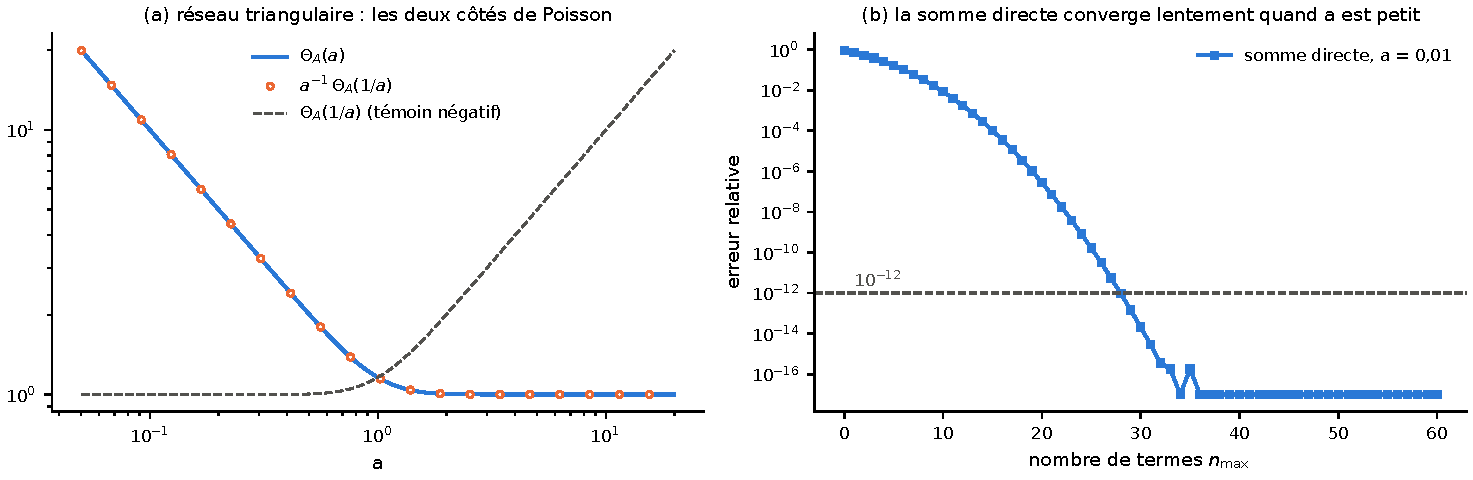
\includegraphics[width=\textwidth]{appF_poisson.pdf}
\caption{Example~1 \tierX. (a) $\Theta_\Lat(a)$ and $a^{-1}\Theta_\Lat(1/a)$ coincide; without the factor $a^{-1}$
(dashed), the curve is wrong. (b) Relative error of the direct sum as a function of the number of terms, for $a=0.01$,
$x=0.3$.}
\label{appF:fig:poisson}
\end{figure}

\begin{exercise}[Example 1]\label{appF:exo1}
(a) Prove the formula in dimension~1 from the Fourier transform of $e^{-\pi ax^2}$, which equals
$a^{-1/2}e^{-\pi\xi^2/a}$. (b) Modify \texttt{theta1} for another even function, $e^{-|x|}$, whose transform is
$2/(1+4\pi^2\xi^2)$, and check the corresponding formula numerically. Why are many more terms needed on the dual side?
\end{exercise}

% =====================================================================================================
\section{Example 2 -- Triangular versus square lattice}\label{appF:ex2}

\paragraph{The question.} At density~1, is the energy per particle $E(L)=\tfrac12\sum_{v\in L\setminus0}V(|v|)$ lower
for the triangular lattice than for the square lattice? We take three potentials that are completely monotone in $r^2$:
\begin{itemize}
\item the Gaussian $e^{-\pi r^2}$, for which $E=(\Theta_L(1)-1)/2$;
\item the Yukawa potential $e^{-\kappa r}/r$, for $\kappa=1$ and $\kappa=2$;
\item the dipolar potential $V=2(1/r-1/\sqrt{r^2+d^2})$, for $d=3$, in the units $U=V/d^2$ of the
\texttt{qf-yukawa-crystal} crate.
\end{itemize}
For these three potentials, the optimality of the triangular lattice is \tierA{} (Chapter~2), conditional on the
upstream theorem \lean{universal_energy_minimum}.

\paragraph{The code.} The dipolar potential decays like $1/r^3$. A sharp cutoff at $|v|<R$ leaves an error of order
$10^{-5}$, even after adding the continuous tail (the output shows it). We therefore cut off smoothly, with a weight
$w=\tfrac12\operatorname{erfc}((r-R)/\sigma)$, and integrate the remainder $(1-w)U$ as a continuum of density~1:
\lstinputlisting[language=Python,style=appFcode,firstline=46,lastline=64,firstnumber=46]{code/examples/python/f02_lattice_energies.py}
\appFsortie{f02_lattice_energies.txt}

\paragraph{Reading the output.} In all three cases, the square costs more. The last column compares with the values
recorded by rusty-SUNDIALS:
\begin{itemize}
\item for Yukawa, with the exact sums of \texttt{exact\_refs.jsonl}, with discrepancies of $10^{-16}$;
\item for the dipolar potential, with the Ewald energies of \texttt{lattice\_gaps.jsonl}, with a discrepancy of
$5\times10^{-13}$.
\end{itemize}
This is the positive control. The negative control recalls a rule about the statements: at equal \emph{spacing}, the
triangular lattice is denser, its energy is higher and the comparison reverses. It is meaningful only at fixed density.
In Figure~\ref{appF:fig:energies}a, the three normalised curves almost coincide and increase without interruption from
$60^\circ$ to $90^\circ$. This is only one path among others in the space of lattices: the theorem concerns all
configurations.

\begin{figure}[ht]\centering
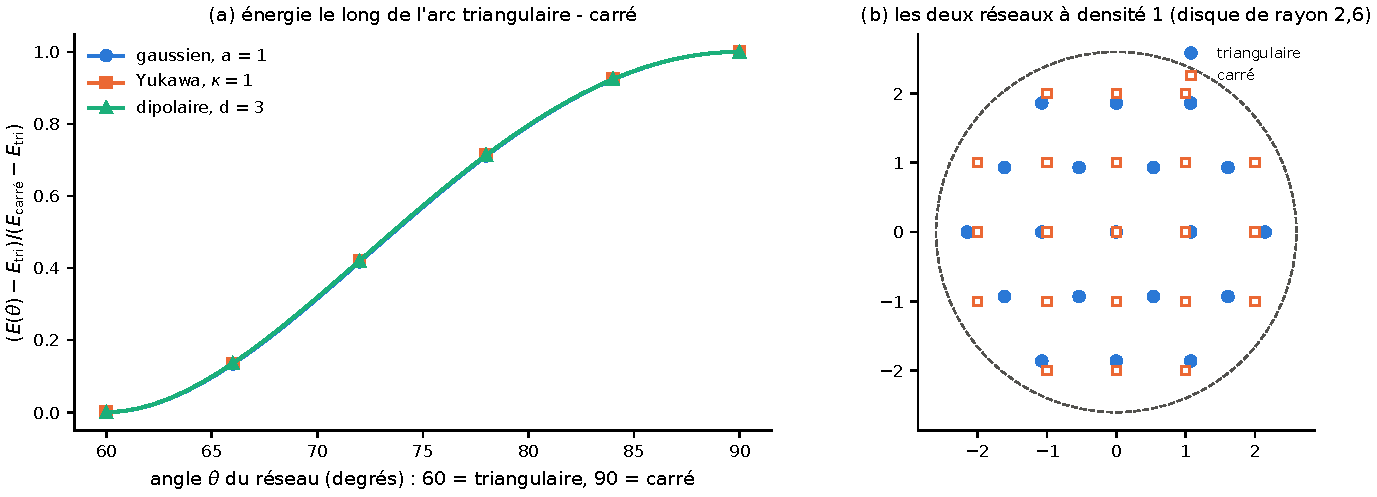
\includegraphics[width=\textwidth]{appF_lattice_energies.pdf}
\caption{Example~2 \tierX. (a) Energy along the lattices of shape $\tau=e^{i\theta}$, normalised between the triangular
($\theta=60^\circ$) and the square ($\theta=90^\circ$) lattice, for the three potentials. (b) The two lattices of
covolume~1.}
\label{appF:fig:energies}
\end{figure}

\begin{exercise}[Example 2]\label{appF:exo2}
(a) Replace \texttt{"gauss"} by a Gaussian $e^{-\pi ar^2}$ with arbitrary parameter $a$, and check on a grid of values of
$a$ that $\Theta_\Lat(a)\le\Theta_{\Z^2}(a)$ (Montgomery's theorem~\cite{app:montgomery}, \tierL). (b) For a potential that is \emph{not}
completely monotone, for instance $V=e^{-r^2}-\tfrac12e^{-r^2/4}$, plot the energy along the same arc. Is the minimum
still at $60^\circ$? What can one conclude from this, and what can one not conclude?
\end{exercise}

% =====================================================================================================
\section[Example 3 -- Complete monotonicity]{Example 3 -- Complete monotonicity: what a computer can say}\label{appF:ex3}

\paragraph{The question.} A function $g$ is completely monotone (CM) if $(-1)^ng^{(n)}(t)\ge0$ for all $n$ and all
$t>0$. A program tests only finitely many pairs $(n,t)$. It can therefore \emph{refute} complete monotonicity, since a
single wrong sign suffices, but never prove it: the proof belongs to the CM/Bernstein library and to the theorem
\lean{ALEXIS} of Chapter~5. What do we see on three CM potentials and on two functions that are not CM?

\paragraph{The code.} \texttt{mpmath.diff} differentiates numerically with 40 significant digits, enough for order~8:
\lstinputlisting[language=Python,style=appFcode,firstline=22,lastline=40,firstnumber=22]{code/examples/python/f03_cm_signs.py}
\appFsortie{f03_cm_signs.txt}

\paragraph{Reading the output.} The three physical potentials pass the $9\times7$ tests. The two counterexamples fail,
and the output says where:
\begin{itemize}
\item $e^{-t}-\tfrac12e^{-2t}$ is a mixture of exponentials whose Bernstein measure $\delta_1-\tfrac12\delta_2$ changes
sign. It fails from $n=2$ on, since $(-1)^ng^{(n)}=e^{-t}-2^{n-1}e^{-2t}<0$ for small $t$.
\item Lennard-Jones fails already at $n=0$: it becomes negative.
\end{itemize}
The first failure is a certificate of non-complete-monotonicity, which can be checked by hand. The successes, for their
part, certify nothing.

\begin{figure}[ht]\centering
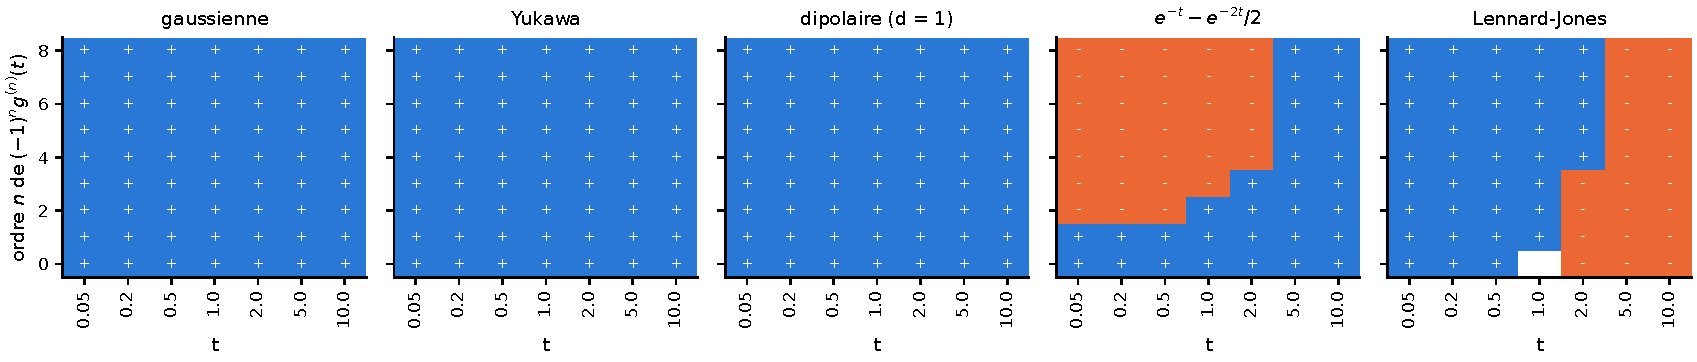
\includegraphics[width=\textwidth]{appF_cm_signs.pdf}
\caption{Example~3 \tierX. Sign of $(-1)^ng^{(n)}(t)$ (blue: $+$, orange: $-$, white: exact zero) for $n\le8$ and seven
values of $t$. The first three potentials are CM (\tierA{} theorems of Chapter~2); the last two are not.}\label{appF:fig:cm}
\end{figure}

\begin{exercise}[Example 3]\label{appF:exo3}
(a) Prove by hand that $e^{-t}-\tfrac12e^{-2t}$ is not CM, starting from the value of $g''(0^+)$. (b) The program says
that $g(t)=e^{-\sqrt t}$ passes all the tests. Prove that it is CM by writing it as $f\circ\phi$, with $f=e^{-s}$ CM and
$\phi=\sqrt{\cdot}$ a Bernstein function (Chapter~1). (c) Add the function $1/(1+t^2)$ to \texttt{FUNCS} and predict,
before running the program, the order $n$ of the first failure.
\end{exercise}

% =====================================================================================================
\section{Example 4 -- Wright--Fisher in exact fractions}\label{appF:ex4}

\paragraph{The question.} In the neutral Wright--Fisher model with $N$ copies of a gene, the next generation is a
binomial draw: $P(i,j)=\binom Nj(i/N)^j(1-i/N)^{N-j}$. The theorem \lean{KAL} (Kolmogorov absorption, \tierA) states
that $P^n(i,N)\to h(i)$ for every harmonic function $h$ with $h(0)=0$ and $h(N)=1$ (and a variance condition). Here
$h(i)=i/N$. Can we see this \emph{exactly}, without rounding? How fast does the convergence take place?

\paragraph{The code.} Python's \texttt{fractions} module computes with exact rationals:
\lstinputlisting[language=Python,style=appFcode,firstline=22,lastline=32,firstnumber=22]{code/examples/python/f04_wright_fisher.py}
\appFsortie{f04_wright_fisher.txt}

\paragraph{Reading the output.} Two equalities are \emph{exact}, not merely to within $10^{-16}$: the matrix is
stochastic and $Ph=h$. With selection ($r=2$), $h(i)=i/N$ is no longer harmonic: this is the negative control. The
denominators grow fast, with 152 digits at $n=60$. The ratio of two successive discrepancies equals
$0.833333333333=1-1/N$, that is, the second eigenvalue of the Wright--Fisher matrix, $\lambda_2=1-1/N$.

\begin{figure}[ht]\centering
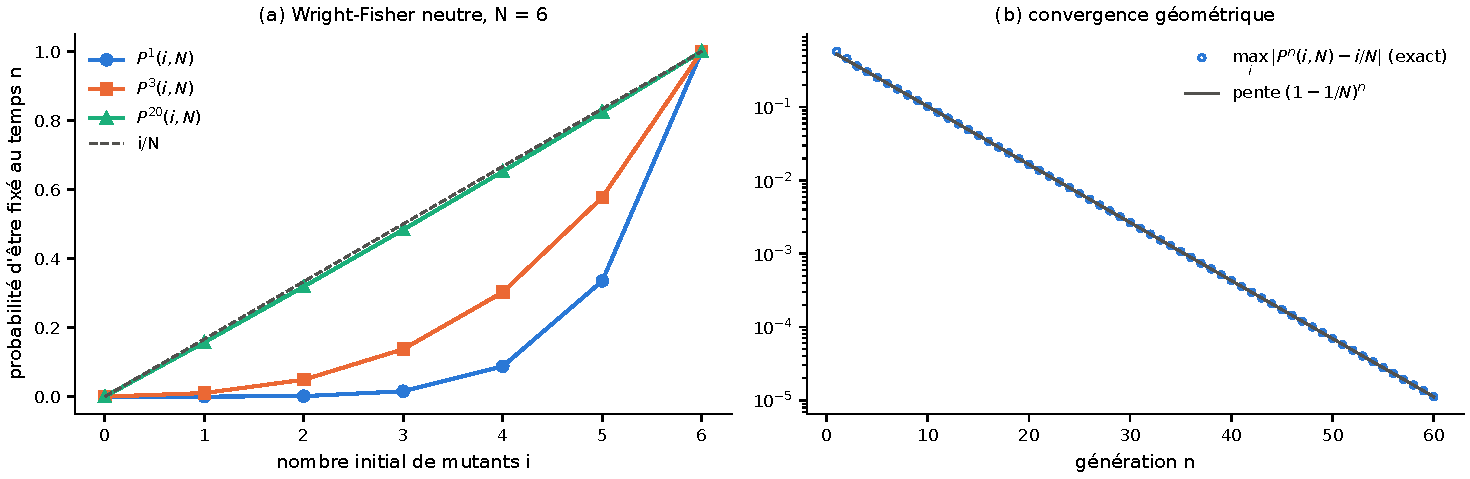
\includegraphics[width=\textwidth]{appF_wright_fisher.pdf}
\caption{Example~4 \tierX. (a) $P^n(i,N)$ for $n=1$, $3$ and $20$, and the limit $i/N$, for $N=6$. (b) The maximal discrepancy,
computed exactly and then converted to floating point, decreases like $(1-1/N)^n$.}\label{appF:fig:wf}
\end{figure}

\begin{exercise}[Example 4]\label{appF:exo4}
(a) Prove that $\lambda_2=1-1/N$ is an eigenvalue of $P$. Hint: apply $P$ to the polynomial $i(N-i)$, after computing
$\mathbb E[X(N-X)]$ for a binomial $X$. (b) Deduce that $|P^n(i,N)-i/N|\le C(1-1/N)^n$. (c) Modify the script for Moran
instead of Wright--Fisher, and compare the rates for equal $N$.
\end{exercise}

% =====================================================================================================
\section{Example 5 -- Isothermal graph versus star}\label{appF:ex5}

\paragraph{The question.} A mutant of fitness $r$ is placed on a vertex of a graph, and the population evolves by
birth--death (the model of N4, Chapter~4). The isothermal theorem \lean{ILENE} (\tierA) states the following: if the
replacement matrix is doubly stochastic, the fixation probability is Moran's, $(1-r^{-1})/(1-r^{-n})$, \emph{whatever}
the starting vertex. What happens on the star, which is not isothermal?

\paragraph{The code.} The state is the set $S$ of mutants, encoded by a bit mask, which gives $2^n$ states. The fixation
probabilities solve a linear system, which we solve in fractions by Gaussian elimination:
\lstinputlisting[language=Python,style=appFcode,firstline=37,lastline=48,firstnumber=37]{code/examples/python/f05_graph_fixation.py}
\lstinputlisting[language=Python,style=appFcode,firstline=51,lastline=76,firstnumber=51]{code/examples/python/f05_graph_fixation.py}
\appFsortie{f05_graph_fixation.txt}

\paragraph{Reading the output.} On the cycle with 4 vertices, which is isothermal, the value is $8/15$ everywhere: it is
Moran's. On the star with 3 vertices we recover the values of N4, all three \tierA{}:
\begin{itemize}
\item $5/12$ for a mutant at the centre;
\item $2/3$ for a mutant on a leaf;
\item $7/12$ for a uniform start, against $4/7$ for Moran.
\end{itemize}
The values of the star with 4 vertices, $392/1265$, $168/253$ and $728/1265$, are only \tierX{} in N4: they come from
an unverified script, and are recovered here by a second script. The last two lines show why the number of mutants is
not a Markov chain on the cycle. With two mutants, the probability of moving up one step is $1/3$ if they are
neighbours and $2/3$ if they are opposite. But the ratio $P^+/P^-$ equals $r=2$ in both cases: this is the
per-configuration bias that N4 proves.

\begin{figure}[ht]\centering
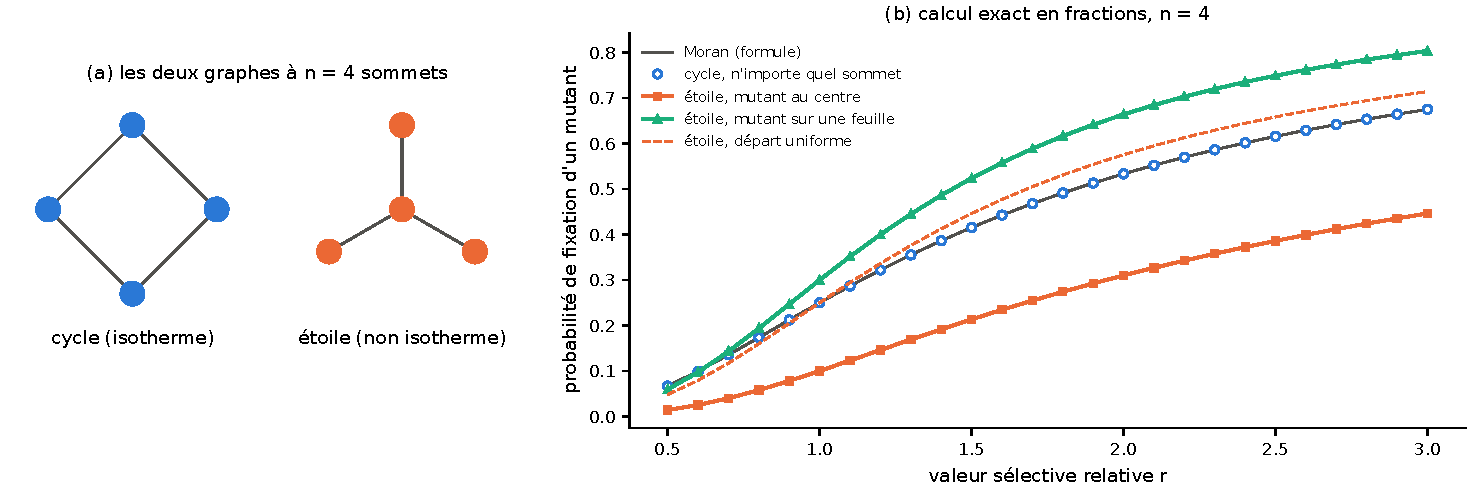
\includegraphics[width=\textwidth]{appF_graph_fixation.pdf}
\caption{Example~5 \tierX, exact computation. (a) The cycle and the star with 4 vertices. (b) Fixation probability of a mutant
as a function of $r$. The cycle follows Moran whatever the vertex. On the star, a mutant at the centre is disadvantaged
and a mutant on a leaf advantaged; on average, the star amplifies selection for $r>1$ in this sample of values.}
\label{appF:fig:graph}
\end{figure}

\begin{exercise}[Example 5]\label{appF:exo5}
(a) Check by hand that, on the star with 3 vertices and $r=2$, the state \texttt{001} (mutant at the centre) moves to
\texttt{011} and to \texttt{101} with probability $1/4$ each, and to the empty state with probability $1/2$. (b) Write
the complete graph $K_4$ (with $W(i,j)=1/3$ for $i\ne j$) and predict the result before running the program. (c) For
the star with $n$ vertices, conjecture the limit of the mean probability as $n\to\infty$, then compare with the
literature (Lieberman, Hauert and Nowak, 2005~\cite{app:lhn}). A conjecture drawn from a few exact values is Tier~X.
\end{exercise}

% =====================================================================================================
\section{Example 6 -- Phonons and zero-point energy}\label{appF:ex6}

\paragraph{The question.} In Chapter~3, conjecture QU-1 asked whether the triangular lattice also minimises the harmonic
zero-point energy $E_{zp}=\tfrac12\langle\omega_1+\omega_2\rangle_{\mathrm{ZB}}$. For the Gaussian $e^{-\pi ar^2}$, the
P2 programme found the opposite (\tierX). On $a\in(0.37668, 1.58148)$, the triangular lattice is a local
\emph{maximum} of $E_{zp}$. Can we recover this with thirty lines of numpy?

\paragraph{The code.} The dynamical matrix $D(\mathbf k)=\sum_{R\ne0}(1-\cos\mathbf k\cdot R)\,\mathrm{Hess}\,V(R)$ is
$2\times2$, so its eigenvalues have a closed form. The average over the Brillouin zone is taken on an $n\times n$ grid
of the reciprocal cell. The fractional grid is the same for all shapes $\tau$, which makes the grid error cancel in the
differences:
\lstinputlisting[language=Python,style=appFcode,firstline=41,lastline=67,firstnumber=41]{code/examples/python/f06_phonons_zero_point.py}
\appFsortie{f06_phonons_zero_point.txt}

\paragraph{Reading the output.} The positive controls are the P2 values. For $a=1$, the script recovers
$E_{zp}(\rho)=1.5033523522$ to within $3\times10^{-8}$ on the grid $n=192$. It also recovers P2's counterexample, the
rhombus $\tau=0.5+0.966025\,i$, lower by $1.3074\times10^{-2}$. The curvature $c(a)$ changes sign as announced:
\begin{itemize}
\item it is negative for $a=0.5$ and $a=1$, where $\rho$ is a local maximum;
\item it is positive for $a=0.25$ and $a=2$, where $\rho$ is a local minimum.
\end{itemize}
The four P2 values are recovered to within one thousandth, and the curvature does not move between grids $48$ and
$96$. All of this remains \tierX: it is a second floating-point computation, not a proof. The B2 certificate of
Chapter~3 treats the case $a=1$ with ball arithmetic.

\begin{figure}[ht]\centering
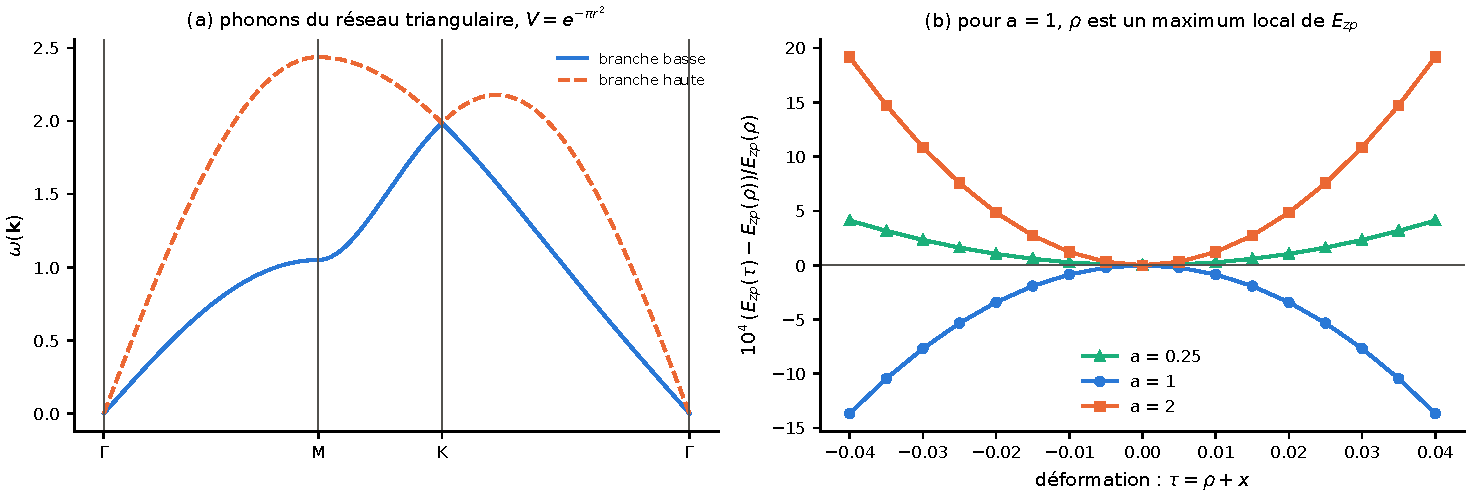
\includegraphics[width=\textwidth]{appF_phonons.pdf}
\caption{Example~6 \tierX. (a) The two phonon branches of the triangular lattice for $V=e^{-\pi r^2}$, along
$\Gamma$--M--K--$\Gamma$; they vanish at $\Gamma$, as for every crystal (acoustic modes). (b) Relative variation of
$E_{zp}$ when $\rho$ is deformed into $\rho+x$: a downward parabola for $a=1$ (local maximum), upward for $a=0.25$ and
$a=2$.}\label{appF:fig:phonons}
\end{figure}

\begin{exercise}[Example 6]\label{appF:exo6}
(a) Prove that $D(\mathbf k)$ is symmetric and that $D(\mathbf 0)=0$. Why is $\omega(\mathbf k)$ linear in
$|\mathbf k|$ near $\Gamma$? (b) Modify \texttt{curvature} to plot $c(a)$ on $a\in[0.3, 1.7]$ and locate numerically
the two sign changes (P2: $0.37668$ and $1.58148$). (c) Why can the statement ``the triangular lattice is a local
maximum of $E_{zp}$ for $a=1$'' not become Tier~A with this code alone?
\end{exercise}

% =====================================================================================================
\section[Example 7 -- CVODE in Rust]{Example 7 -- CVODE in Rust: a stiff ODE, then the Kolmogorov equation}\label{appF:ex7}

\paragraph{The question.} rusty-SUNDIALS is a Rust rewrite of SUNDIALS. Its CVODE solver integrates stiff differential
equations with the BDF formulas. How is it called from an independent crate? And why does an explicit scheme fail where
BDF succeeds?

\paragraph{A stiff ODE.} The Prothero--Robinson problem, $y'=\lambda(y-\cos t)-\sin t$ with $y(0)=2$ and
$\lambda=-10^4$, has the exact solution $y=\cos t+e^{\lambda t}$. Here is the call to CVODE (a function of the crate's
library):
\lstinputlisting[language=Rust,style=appFcode,firstline=36,lastline=68,firstnumber=36]{code/examples/rust/src/lib.rs}
\appFsortie{f07a_tb_stiff.txt}

\paragraph{Reading the output.} CVODE follows the exact solution to within $6\times10^{-9}$ during the transient phase,
where $e^{\lambda t}$ dies out within $10^{-4}$, then to within $3\times10^{-11}$ up to $t=10$. It gets there in 506
steps. The explicit Euler scheme is stable only if $|1+h\lambda|\le1$, that is, $h\le2/|\lambda|=2\times10^{-4}$:
\begin{itemize}
\item with $h=10^{-4}$ it succeeds, but in $10\,000$ steps;
\item with $h=2.5\times10^{-4}$, the error is multiplied by $|1+h\lambda|=1.5$ at each step, reaches $4\times10^{17}$
in 100 steps and ends in \texttt{NaN}.
\end{itemize}
This is the negative control, and the very definition of stiffness.

\begin{uniremark}\tierL{} The BDF formulas of orders~1 and~2 are A-stable: their stability region contains the whole
left half-plane, so they accept any step $h>0$ on $y'=\lambda y$ with $\operatorname{Re}\lambda<0$. By Dahlquist's
second barrier, no A-stable linear multistep method has order greater than~2; the higher-order BDF formulas used by CVODE
(up to order~5) are only $A(\alpha)$-stable, with a stability sector that narrows as the order grows. CVODE varies both the step
size and the order (1 to 5) during an integration~\cite{app:sundials} (standard).\end{uniremark}

\paragraph{Moran's Kolmogorov equation.} The Moran chain (Chapter~4), uniformised in continuous time, obeys
$\dot\pi=\pi(P-I)$. The mass absorbed at $N$ tends to the fixation probability $\varphi_i=(1-r^{-i})/(1-r^{-N})$. The
Jacobian is the constant matrix $(P-I)^{\mathsf T}$. We double the output time until the interior mass falls below
$10^{-12}$:
\lstinputlisting[language=Rust,style=appFcode,firstline=125,lastline=172,firstnumber=125]{code/examples/rust/src/lib.rs}
\appFsortie{f07b_tb_moran_forward.txt}

\paragraph{Reading the output.} For $N=3$, $r=2$ and $i=1$, CVODE gives $4/7$ to within $9.5\times10^{-14}$. For
$N=10$, the 27 values ($r=0.8$, $1$ and $1.5$, $i=1,\dots,9$) follow the formula to within $10^{-12}$. The two negative
controls are refused:
\begin{itemize}
\item the identity kernel, which never absorbs;
\item the formula with the inverted exponent, which gives $1/7$.
\end{itemize}
The \texttt{qf-popgen} crate of Chapter~5 does the same computation with a more complete absorption certificate. It is
not yet merged into \texttt{main}, which is why this crate rewrites the equation directly.

\begin{figure}[ht]\centering
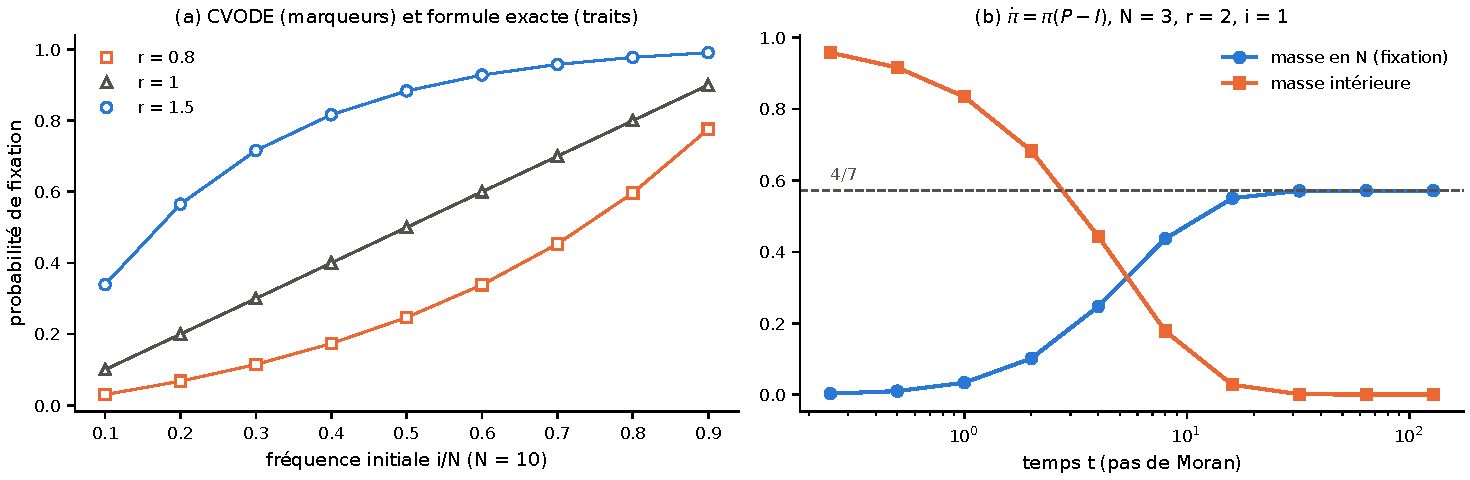
\includegraphics[width=\textwidth]{appF_rust_moran.pdf}
\caption{Example~7 \tierX, plotted from the CSV files written by \texttt{tb\_moran\_forward}. (a) Fixation probability
for $N=10$: CVODE (markers) and exact formula (lines). (b) $N=3$, $r=2$, $i=1$: the mass at $N$ rises towards $4/7$ and
the interior mass dies out, at the output times $0.25\cdot2^k$.}\label{appF:fig:moran}
\end{figure}

\begin{exercise}[Example 7]\label{appF:exo7}
(a) For $y'=\lambda y$, show that the implicit Euler scheme (BDF of order~1) gives $y_{n+1}=y_n/(1-h\lambda)$, which is
stable for every $h>0$ if $\lambda<0$. (b) Why does the interior mass decay exponentially, and what rate should be
expected for $N=3$, $r=2$? Compute the eigenvalues of the restriction of $P-I$ to the interior states. (c) Add a
control: a kernel one of whose rows sums to $1.001$. Which quantity computed by \texttt{absorb} detects it?
\end{exercise}

% =====================================================================================================
\section{Example 8 -- Relaxing a small Yukawa crystal}\label{appF:ex8}

\paragraph{The question.} 64 particles interact via $e^{-2r}/r$ in a periodic box. If they are released from an
arbitrary position and descend the energy gradient ($\dot x=F(x)$), do they recover the triangular lattice? The theorem
says only that the triangular lattice is the \emph{global minimum} (\tierA, conditional). It does not say that the
descent reaches it.

\paragraph{The code.} The crate calls the API of \texttt{qf-yukawa-crystal}:
\begin{itemize}
\item \texttt{ExactBox} for the energy, the forces and the Hessian summed over the images up to $R=12$;
\item \texttt{lattice\_energy\_exact} for the exact energy of the lattice.
\end{itemize}
The relaxation itself is a CVODE integration whose Jacobian is minus the Hessian (function \texttt{relax\_traced} of the
library). Here is the main program:
\lstinputlisting[language=Rust,style=appFcode,firstline=60,lastline=105,firstnumber=60]{code/examples/rust/src/bin/tb_yukawa_relax.rs}
\appFsortie{f08_tb_yukawa_relax.txt}

\paragraph{Reading the output.} The three starts behave as expected.
\begin{itemize}
\item \emph{Perturbed triangular lattice} (positive control): it returns to the exact lattice energy, to within
$10^{-16}$. This energy, $0.393542848871227$ at $R=12$, differs by $6\times10^{-11}$ from the value at $R=20$ recorded in
\texttt{exact\_refs.jsonl}, which is $0.39354284893239$; this is the omitted tail.
\item \emph{Random start}: it stops $2.1\times10^{-3}$ \emph{above}, at a stationary point (forces below $10^{-9}$) that
has defects (Figure~\ref{appF:fig:yukawa}b). We did not check the Hessian: nothing here says that it is a local
minimum. A gradient descent does not always find the global minimum.
\item \emph{Square lattice in a square box} (negative control): it descends below the energy of the square lattice,
which indicates that the square lattice is not a minimum, but it remains above the triangular lattice, which the
$8\times8$ box cannot contain.
\end{itemize}

\begin{figure}[ht]\centering
\includegraphics[width=\textwidth]{appF_rust_yukawa.pdf}
\caption{Example~8 \tierX. (a) Energy per particle above the triangular lattice during the CVODE relaxation, at the
output times $0.01\cdot2^k$. (b) Final state of the random start: triangular domains and defects. (c) Final state in the
square box.}\label{appF:fig:yukawa}
\end{figure}

\begin{exercise}[Example 8]\label{appF:exo8}
(a) Why can the box $8a\times4\sqrt3\,a$ contain exactly the $8\times8$ triangular lattice of spacing $a$, whereas the
$8\times8$ box cannot? (b) Change the seed of the random start (11) to five other values. How many starts reach the
triangular lattice to within $10^{-10}$? (c) Does this result contradict the theorem?
\end{exercise}

% =====================================================================================================
\section{Example 9 -- The invariants of the \texorpdfstring{$\sigma=3$}{sigma=3} shell model}\label{appF:ex9}

\paragraph{The question.} The shell model of Section~\ref{ch5:U4} conserves two quantities:
\begin{itemize}
\item $S=\sum|v_n|^2$;
\item $H_3$, whose quadratic part equals $2D\Omega$, where $\Omega$ is the enstrophy.
\end{itemize}
Lean deduces from them the bound $2D\,\Omega(t)\le H_3(0)+S(0)^{3/2}$ along solutions (\tierAs, Chapter~5). Does a
numerical integrator conserve these invariants? And does the bound hold along a trajectory?

\paragraph{The code.} Six shells, $D=0.05$, integration up to $T=2$ with \texttt{integrate\_cvode} of
\texttt{qf-shell-cascade}, which evaluates the invariants at each internal CVODE step. The negative control multiplies
one coupling by $1+10^{-2}$:
\lstinputlisting[language=Rust,style=appFcode,firstline=18,lastline=63,firstnumber=18]{code/examples/rust/src/bin/tb_shell_sigma3.rs}
\appFsortie{f09_tb_shell_sigma3.txt}

\paragraph{Reading the output.} For the exact model, the invariants drift by $5\times10^{-10}$ for $S$ and by
$9\times10^{-8}$ for $H_3$, relative to the scale of its terms. These drifts come from the solver tolerance, not from
the model. The Lean bound is far from attained, with a maximal ratio of $0.29$. With the perturbed coupling, the drifts
rise to $3$ and $4\times10^{-3}$: conservation rests on the exact cancellation of the nonlinear terms, which the negative
control breaks. We restrict ourselves to six shells: the fastest rotation, $\omega_n=Dk_n^3$ with $k_n=2^n$, is
multiplied by~8 with each added shell, and CVODE must resolve it step by step.

\begin{figure}[ht]\centering
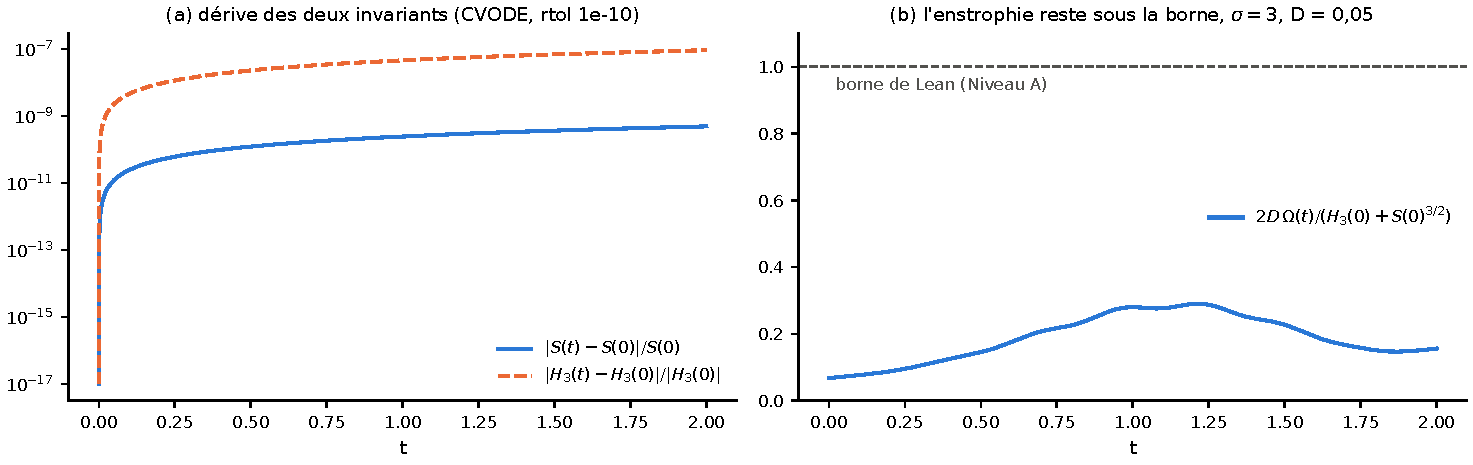
\includegraphics[width=\textwidth]{appF_rust_shell.pdf}
\caption{Example~9 \tierX, plotted from the CSV written by \texttt{tb\_shell\_sigma3} (one internal step in twenty).
(a) Relative drift of the two invariants. (b) The ratio $2D\Omega(t)/(H_3(0)+S(0)^{3/2})$ stays below~1, as the Lean
theorem requires.}\label{appF:fig:shell}
\end{figure}

\begin{exercise}[Example 9]\label{appF:exo9}
(a) Prove that $\frac{d}{dt}\sum|v_n|^2=0$ for the model without dissipation. Group the coupling terms in pairs.
(b) Replace \texttt{sigma: 3.0} by \texttt{2.0}. Are the invariants $S$ and $H_2$ still conserved? Why does the
enstrophy bound no longer follow in the same way?
\end{exercise}

% =====================================================================================================
\section[Example 10 -- LeanFlow]{Example 10 -- LeanFlow: certifying fractions, rejecting a lie}\label{appF:ex10}

\paragraph{The question.} Example~\ref{appF:ex5} computed in Python the exact table of fixation probabilities of the
star with 3 vertices. Python can make mistakes, or be badly programmed. How can these fractions be checked by the Lean
kernel, without writing a single line of Lean?

\paragraph{The code.} LeanFlow's \texttt{lean.certify} receives claims about rationals. It translates them into
statements about integers, has them decided by \lean{decide +kernel} (tactic \texttt{decide\_kernel}), then audits
\texttt{\#print axioms}. An exact Python oracle must return the same verdict as the kernel; otherwise the result is an
error, never a success. Here is the construction of the claim ``the table $x_S$ is harmonic'':
\lstinputlisting[language=Python,style=appFcode,firstline=34,lastline=49,firstnumber=34]{code/examples/python/f10_leanflow_certify.py}
\appFsortie{f10_leanflow_certify.txt}
Here is the shorter of the two generated certificates, as the kernel decided it:
\lstinputlisting[language=Lean,style=appFcode]{code/examples/lean/f10_generated_PosMeanAboveMoran.lean}

\paragraph{Reading the output.} The two true claims are accepted:
\begin{itemize}
\item the six first-step equations, satisfied exactly by the table $(0,\tfrac5{12},\tfrac23,\tfrac56,
\tfrac23,\tfrac56,\tfrac{14}{15},1)$;
\item the inequality $7/12>4/7$.
\end{itemize}
The two planted claims are rejected, with \lean{sorryAx} in the list of axioms:
\begin{itemize}
\item the Moran vector $(0,\tfrac47,\tfrac67,1)$ indexed by $|S|$ violates the six interior equations, but it satisfies
the two boundary conditions (\texttt{cert\_0} and \texttt{cert\_1} are not refused);
\item the reversed inequality $7/12<4/7$ is refused.
\end{itemize}
LeanFlow checks only \texttt{\#print axioms}, which can be fooled (Chapter~2). The script therefore completes the Tier~A
gate. Each accepted source is recompiled to \texttt{.olean} with Lean~4.34.1 and then replayed by \texttt{leanchecker},
with exit code~0 for both. None of the words \texttt{skipKernelTC}, \texttt{addDecl}, \texttt{native\_decide} or
\texttt{implemented\_by} occurs in them. The replay control, a nonexistent module, exits with code~1. The two
certificates are therefore \tierA, but for the \emph{arithmetic statement only}. That this table is the fixation
probability of the star requires in addition the uniqueness of the harmonic solution (Chapter~4) and the identification
of the Python transitions with those of \lean{bdK}. This link is a human argument, \tierC.

\begin{exercise}[Example 10, LeanFlow]\label{appF:exo10}
(a) Certify in the same way the table of the cycle with 4 vertices ($2^4$ states, value $8/15$ for every single
mutant). (b) Plant a one-ulp error: replace $5/12$ by the fraction of the float \texttt{float(5/12)}. Does LeanFlow
accept it? Why is a certificate on rationals more demanding than a floating-point comparison to within $10^{-15}$?
\end{exercise}

% =====================================================================================================
\section{Example 11 -- Reading and checking the theorem ILENE}\label{appF:ex11}

\paragraph{The question.} Chapter~5 cites \lean{ILENE}, the single-mutant version of the isothermal theorem. How can the
reader see, on their own machine, the exact statement that Lean checked and the axioms its proof depends on? And how
can a real proof be told apart from a fake one?

\paragraph{The code.} A 21-line file, of which we reproduce lines 2 to 21, imports the compiled module and asks Lean four questions:
\lstinputlisting[language=Lean,style=appFcode,firstline=2,firstnumber=2]{code/examples/lean/f11_ilene.lean}
(The first line of the file, the \texttt{import} of the acronym module, is omitted here.)
It is compiled with Lean~4.34.1 and Mathlib \texttt{d13f23b7}, through the script \texttt{lean\_pinned.py} of the
directory \texttt{scripts/certified\_numerics/}. It gives:
\appFsortie{f11_ilene.txt}

\paragraph{Reading the output.} The output is read in four steps.
\begin{itemize}
\item \texttt{\#check} displays the full statement. The hypotheses are: $0<n$, $0<r$, $r\ne1$, $W$ isothermal and
strongly connected. The conclusion is a limit, that of $P^t(\{v\},V)$ to $(1-r^{-1})/(1-r^{-n})$, for every vertex $v$.
\item The axioms are exactly those of the whitelist. The acronyms module and its sources were replayed by
\texttt{leanchecker}, with exit code~0 (record \texttt{acronymes\_leanchecker.json}): \lean{ILENE} is therefore \tierA.
\item The \texttt{example} checks, by \lean{norm_num}, that the limit value equals $8/15$ for $n=4$ and $r=2$. This is
the value of the cycle of Example~\ref{appF:ex5}.
\item The planted witness asserts a false value, $4/7$, ``proved'' by \lean{sorry}. The file compiles all the same, with
exit code~0 and a mere warning. Only the \texttt{\#print axioms} line betrays the fraud: it displays \lean{sorryAx}.
\end{itemize}
This is the lesson of Chapter~2: a zero exit code proves nothing; one must read the axioms and replay the kernel.

\begin{exercise}[Example 11, Lean]\label{appF:exo11}
(a) Add \texttt{\#check @KAL} and \texttt{\#print axioms AURELIA}, and reread the statements with the help of the table
of acronyms (Section~\ref{ch5:acronymes}). (b) Replace \lean{by sorry} by \lean{by norm_num} in the planted witness.
What does Lean answer, and with which exit code? (c) Why is the equality $1/2=2^{-1}$, used implicitly when comparing
the \texttt{example} with the statement of \lean{ILENE}, a link to be checked, and how can this be done in Lean?
\end{exercise}

% =====================================================================================================
\section{Example 12 -- Cross-check: CVODE versus SciPy}\label{appF:ex12}

\paragraph{The question.} Two codes written by the same team can share the same error. Are the numbers of
Example~\ref{appF:ex7} confirmed by \emph{independent} methods?

\paragraph{The code.} The script rereads the outputs of the Rust binary and recomputes the same quantities in two ways:
\begin{itemize}
\item for the stiff problem, with SciPy's Radau method, an implicit Runge--Kutta method and not BDF;
\item for Moran, with the matrix exponential $\pi(t)=e_i\,e^{t(P-I)}$, without any time step.
\end{itemize}
\lstinputlisting[language=Python,style=appFcode,firstline=56,lastline=78,firstnumber=56]{code/examples/python/f12_scipy_crosscheck.py}
\appFsortie{f12_scipy_crosscheck.txt}

\paragraph{Reading the output.} After the transient phase, CVODE and Radau agree to within $3\times10^{-11}$. At the
first two instants, the discrepancy of $5\times10^{-9}$ is that of CVODE from the exact solution: the Radau value
coincides with $\cos t+e^{\lambda t}$, and the CVODE tolerance was $10^{-8}$. For Moran, CVODE and the matrix exponential
agree to within $1.3\times10^{-11}$ at the ten output times. The negative control shifts one time by $10^{-3}$, and the
discrepancy, of $8\times10^{-4}$, becomes immediately visible: the comparison therefore has the power to detect an
error.

\begin{exercise}[Example 12]\label{appF:exo12}
(a) Replace \texttt{method="Radau"} by \texttt{"RK45"}, an explicit method. How many evaluations are needed, and why?
(b) For Moran, the matrix exponential is exact up to rounding. Why does it not replace CVODE for $N=1000$?
\end{exercise}

% =====================================================================================================
\section{Summary}\label{appF:bilan}

The twelve examples were run on 2026-10-26, and all their controls behaved as expected. They illustrate the three ways
of handling a number in this book.
\begin{itemize}
\item \emph{Floating-point computation} (Examples~1, 2, 3, 6 to 9 and 12) explores, checks and refutes. It recovers the
published values to the expected precision, but it remains Tier~X.
\item \emph{Exact rational computation} (Examples~4 and~5) removes rounding, but not the risk of a programming error.
\item \emph{The Lean kernel} (Examples~10 and~11) removes that risk for the checked statement, and for it alone. The link
between that statement and the question asked remains a link to be checked separately.
\end{itemize}

\backmatter
\begin{thebibliography}{99}
\IfFileExists{refs_ch1.tex}{\bibitem{oai} OpenAI, \emph{Universal optimality of the triangular lattice}, OpenAI Math Release preprint, 2026-09-23, \url{https://github.com/openai/math}, commit \texttt{fd4aeeb2ee4fc729c18d98444fed42fd0529eeeb}. AI-generated; not peer reviewed. Statement read in the pinned copy of the repository.
\bibitem{ckmrv} H.~Cohn, A.~Kumar, S.~D.~Miller, D.~Radchenko, M.~Viazovska, Universal optimality of the $E_8$ and Leech lattices and interpolation formulas, Ann.\ of Math.\ 196 (2022) 983--1082, doi:10.4007/annals.2022.196.3.3; arXiv:1902.05438. Cited from the bibliography of doi:10.5281/zenodo.23646105; reading not recorded by the author of this chapter.
\bibitem{ck} H.~Cohn, A.~Kumar, Universally optimal distribution of points on spheres, J.\ Amer.\ Math.\ Soc.\ 20 (2007) 99--148, doi:10.1090/S0894-0347-06-00546-7. Reading not recorded.
\bibitem{viazovska} M.~S.~Viazovska, The sphere packing problem in dimension 8, Ann.\ of Math.\ 185 (2017) 991--1015, doi:10.4007/annals.2017.185.3.7. Reading not recorded.
\bibitem{montgomery} H.~L.~Montgomery, Minimal theta functions, Glasgow Math.\ J.\ 30 (1988) 75--85, doi:10.1017/S0017089500007047. Cited at second hand, through K.~Deng and S.~Luo (arXiv:2411.17199); the original was not opened.
\bibitem{bernstein} S.~Bernstein, Sur les fonctions absolument monotones, Acta Math.\ 52 (1929) 1--66, doi:10.1007/BF02592679. Cited at second hand; the original was not opened.
\bibitem{widder} D.~V.~Widder, The Laplace Transform, Princeton University Press, 1941. Not consulted; cited from the bibliographies of Mathlib and Cohn--Kumar 2007.
\bibitem{lean4} L.~de~Moura, S.~Ullrich, The Lean 4 theorem prover and programming language, in Automated Deduction -- CADE 28, LNCS 12699, Springer (2021) 625--635, doi:10.1007/978-3-030-79876-5\_37. Reading not recorded.
\bibitem{mathlib} The mathlib Community, The Lean mathematical library, Proc.\ CPP 2020, ACM (2020) 367--381, doi:10.1145/3372885.3373824. Reading not recorded.
\bibitem{elenchus} X.~Callens, SocrateAI-Scientific-Elenchus, \url{https://github.com/xaviercallens/SocrateAI-Scientific-Elenchus} (commit \texttt{c9ae8cd}).
\bibitem{v1} X.~Callens, \emph{The Triangular Lattice and Universal Optimality} (textbook, version 1), Zenodo (2026), doi:10.5281/zenodo.23295142.
\bibitem{p3} X.~Callens, \emph{Completely monotone and Bernstein functions in Lean~4: a kernel-checked library with a general subordination theorem, applied to planar universal optimality}, preprint v1, doi:10.5281/zenodo.23653842 (2026). Produced by AI agents; not peer reviewed.
\bibitem{a2} X.~Callens, Audit A2 of the openai/NavierStokesAndEuler corpus: rebuild, kernel replay and axiom audit, record \texttt{results/proposal2/2026-10-26/A2/}; preprint v1, doi:10.5281/zenodo.23661381 (2026). Produced by AI agents; not peer reviewed.
}{}
\IfFileExists{refs_ch2.tex}{% References of chapter 2 (\bibitem only, inserted into thebibliography).
% Each entry is copied from the bibliography of a source paper of the chapter, with its caveats.
% Keys are prefixed with ch2 to avoid collisions with other chapters.
\bibitem{ch2oaiss} OpenAI, \emph{Triangular minimality for planar Coulomb renormalized energy} (preprint dated
2026-09-23), in the OpenAI Math release, github.com/openai/math (checkout HEAD \texttt{adc7f124\ldots}), folder
\texttt{preprints/Triangular-minimality-for-planar-Coulomb-}\allowbreak\texttt{renormalized-energy-September-23-2026}. Produced by an AI;
not peer reviewed. (Source: bibliography of doi\string:10.5281/zenodo.23653827.)
\bibitem{ch2ps} M.~Petrache, S.~Serfaty, \emph{Crystallization for Coulomb and Riesz interactions as a consequence of the
Cohn--Kumar conjecture}, arXiv:1908.09714v3 (2019).
\bibitem{ch2dip} X.~Callens, \emph{The bilayer dipolar-exciton interaction is completely monotone in $r^2$:
kernel-checked triangular-lattice corollaries at every density and an exact-Ewald CVODE consistency study}, preprint v1,
doi\string:10.5281/zenodo.23646103 (2026). Produced by AI agents; not peer reviewed.
\bibitem{ch2yuk} X.~Callens, \emph{The triangular lattice minimises the planar Yukawa energy at every density and for every finite mixture of screening lengths: kernel-checked corollaries of planar universal optimality, a human proof, and an exact-potential CVODE consistency study}, preprint v1,
doi\string:10.5281/zenodo.23646105 (2026). Produced by AI agents; not peer reviewed.
\bibitem{ch2kel} X.~Callens, \emph{The Rytova--Keldysh interaction is a positive Gaussian mixture: kernel-checked
admissibility for planar universal optimality and Keldysh-jellium Madelung energies of TMD Wigner lattices}, preprint v1,
doi\string:10.5281/zenodo.23646107 (2026). Produced by AI agents; not peer reviewed.
\bibitem{ch2ssa} X.~Callens, \emph{The Sandier--Serfaty triangular-lattice conjecture: an independent reproduction of a
claimed finite certificate, an adversarial audit of the claimed reduction, and a Lean statement (no proof of the
conjecture is claimed)}, preprint v1, doi\string:10.5281/zenodo.23653827 (2026). Produced by AI agents; not peer
reviewed.
\bibitem{ch2ssl} X.~Callens, \emph{Toward a machine-checked proof of the claimed Sandier--Serfaty certificate: 4 of 12
stages re-executed in the Lean kernel, one reduction lemma proved, and the measured cost of the rest (a partial
formalization; the conjecture is not formally proved)}, preprint v1, doi\string:10.5281/zenodo.23656804 (2026). Produced by
AI agents; not peer reviewed.
\bibitem{ch2b3} X.~Callens, \emph{Can the planar Sandier--Serfaty proof architecture reach three-dimensional bcc
jellium? A feasibility study with a negative outcome}, preprint v1, doi\string:10.5281/zenodo.23655002 (2026). Produced by
AI agents; not peer reviewed.
\bibitem{ch2ss} E.~Sandier, S.~Serfaty, \emph{From the Ginzburg--Landau model to vortex lattice problems}, Comm.\ Math.\
Phys.\ \textbf{313} (2012) 635--743; arXiv:1011.4617v2.
\bibitem{ch2bs} L.~B\'etermin, E.~Sandier, \emph{Renormalized energy and asymptotic expansion of optimal logarithmic
energy on the sphere}, arXiv:1404.4485v5 (2018).
\bibitem{ch2bhs} J.~S. Brauchart, D.~P. Hardin, E.~B. Saff, \emph{The next-order term for optimal Riesz and logarithmic
energy asymptotics on the sphere}, Contemp.\ Math.\ \textbf{578} (2012) 31--61; arXiv:1202.4037v1.
\bibitem{ch2mn} C.~B. Muratov, M.~Novaga, \emph{BCC optimality for the three-dimensional Coulomb lattice energy}, arXiv:2610.29732v1. (Read in full text for doi\string:10.5281/zenodo.23655002:
Theorem~1, p.~4; Proposition~6, p.~13; p.~3 and Section~7, p.~14.)
\bibitem{ch2bhr} T.~C. Berkelbach, M.~S. Hybertsen, D.~R. Reichman, \emph{Theory of neutral and charged excitons in
monolayer transition metal dichalcogenides}, arXiv:1305.4972v1 (2013).
\bibitem{ch2dlmf} NIST Digital Library of Mathematical Functions, \S11.2 (eq.~11.2.5) and \S11.5 (eq.~11.5.2),
\url{https://dlmf.nist.gov/11}, accessed 2026-10-25.
\bibitem{ch2ssv} R.~L. Schilling, R.~Song, Z.~Vondra\v{c}ek, \emph{Bernstein Functions: Theory and Applications},
2nd ed., de Gruyter, 2012. Existence of the monograph confirmed by its publisher's record; its composition theorem
was \emph{not} consulted or located.
}{}
\IfFileExists{refs_ch3.tex}{% References of chapter 3 (\bibitem entries only; the thebibliography environment is opened by references.tex).
% Keys prefixed ch3-. The "not read" notes faithfully repeat the records of the source papers.
\bibitem{ch3-p2zp} X.~Callens, \emph{Does the triangular lattice minimise the harmonic zero-point energy? A numerical
counterexample for completely monotone potentials, with kernel-checked curvature identities}, preprint v1,
doi:10.5281/zenodo.23653833 (2026). Not peer reviewed; audited by a separate AI agent, no human audit.
\bibitem{ch3-b2} X.~Callens, \emph{The triangular lattice is not a local minimum of the harmonic zero-point energy for
$e^{-\pi r^2}$: a certified linear-response majorant along a symmetric shear}, preprint v1,
doi:10.5281/zenodo.23655392 (2026). Not peer reviewed; audited by a separate AI agent, no human audit.
\bibitem{ch3-b1} X.~Callens, \emph{The harmonic triangular-to-oblique instability of the quantum Gaussian-core crystal:
first order, near the Lindemann melting estimate, and absent in the self-consistent harmonic approximation. A
preregistered negative result}, preprint v1, doi:10.5281/zenodo.23655625 (2026). Not peer reviewed.
\bibitem{ch3-bsk} X.~Callens, \emph{The Bogoliubov structure factor under the dual-scale envelope $\sqrt{k/2k_*}$:
kernel-checked shape theorems, a one-sided diffraction test, and a Gross--Pitaevskii linear-response check in
rusty-SUNDIALS}, preprint v1, doi:10.5281/zenodo.23646117 (2026). Not peer reviewed.
\bibitem{ch3-fb} X.~Callens, \emph{The Feynman--Bijl single-mode bound in Lean, and a diffraction test of the Bogoliubov
envelope on published structure factors of superfluid $^4$He and trapped Bose gases}, preprint v1,
doi:10.5281/zenodo.23653846 (2026). Not peer reviewed.
\bibitem{ch3-dengluo} K.~Deng, S.~Luo, \emph{Minimizing lattice energy and hexagonal crystallization},
arXiv:2411.17199v1 (2024); Theorem~A cited and checked by the Elenchus citation gate.
\bibitem{ch3-luowei} S.~Luo, J.~Wei, \emph{On lattice hexagonal crystallization for non-monotone potentials},
arXiv:2302.05042v1 (2023); Corollary~1.1 and Lemma~3.5 cited and checked. Journal version (J.\ Math.\ Phys.\
\textbf{65}, 071901, 2024) not opened.
\bibitem{ch3-arb} F.~Johansson, \emph{Arb: efficient arbitrary-precision midpoint-radius interval arithmetic},
arXiv:1611.02831 (2016).
\bibitem{ch3-astra} G.~E. Astrakharchik, J.~Boronat, I.~L. Kurbakov, Yu.~E. Lozovik, \emph{Quantum phase transition in a
two-dimensional system of dipoles}, Phys.\ Rev.\ Lett.\ \textbf{98}, 060405 (2007); arXiv:cond-mat/0608246v2 (read,
quotations checked word for word).
\bibitem{ch3-prestipino} S.~Prestipino, A.~Sergi, E.~Bruno, \emph{Freezing of soft-core bosons at zero temperature: a
variational theory}, Phys.\ Rev.\ B \textbf{98}, 104104 (2018); arXiv:1809.07515v1 (read, quotations checked).
\bibitem{ch3-henkel} N.~Henkel, R.~Nath, T.~Pohl, \emph{Three-dimensional roton excitations and supersolid formation in
Rydberg-excited Bose--Einstein condensates}, Phys.\ Rev.\ Lett.\ \textbf{104}, 195302 (2010); arXiv:1001.3250v2 (read,
quotations checked).
\bibitem{ch3-zeiher} J.~Zeiher, R.~van Bijnen, P.~Schau\ss, S.~Hild, J.-y.~Choi, T.~Pohl, I.~Bloch, C.~Gross,
\emph{Many-body interferometry of a Rydberg-dressed spin lattice}, arXiv:1602.06313v3, doi:10.1038/nphys3835 (2016)
(read, quotations checked).
\bibitem{ch3-db} R.~J. Donnelly, C.~F. Barenghi, \emph{The observed properties of liquid helium at the saturated vapor
pressure}, J.\ Phys.\ Chem.\ Ref.\ Data \textbf{27}, 1217 (1998); web edition, chapter~14, table~14.1 (only
the web edition was read; secondary compilation; \texttt{pages.uoregon.edu/rjd/vapor15.htm}). Primary data: H.~N.~Robkoff, R.~B.~Hallock, Phys.\ Rev.\ B \textbf{24}, 159 (1981); E.~C.~Svensson et al., Phys.\ Rev.\ B \textbf{21}, 3638 (1980).
\bibitem{ch3-godfrin} H.~Godfrin, K.~Beauvois, A.~Sultan, E.~Krotscheck, J.~Dawidowski, B.~F{\aa}k, J.~Ollivier,
\emph{The dispersion relation of Landau elementary excitations and the thermodynamic properties of superfluid $^4$He},
arXiv:2012.09067v1 (2020) ($c=238.3\pm0.1$~m/s at saturated vapour pressure, Sect.~II~A; $m_4=4.0026032$~g/mol).
\bibitem{ch3-sk} D.~M. Stamper-Kurn, A.~P. Chikkatur, A.~G\"orlitz, S.~Inouye, S.~Gupta, D.~E. Pritchard, W.~Ketterle,
\emph{Excitation of phonons in a Bose--Einstein condensate by light scattering}, Phys.\ Rev.\ Lett.\ \textbf{83}, 2876
(1999); arXiv:cond-mat/9906035v2.
\bibitem{ch3-st} J.~Steinhauer, R.~Ozeri, N.~Katz, N.~Davidson, \emph{Excitation spectrum of a Bose--Einstein
condensate}, Phys.\ Rev.\ Lett.\ \textbf{88}, 120407 (2002); arXiv:cond-mat/0111438v1.
\bibitem{ch3-feynman} R.~P. Feynman, Phys.\ Rev.\ \textbf{94}, 262 (1954); A.~Bijl, Physica \textbf{7}, 869 (1940);
N.~N. Bogoliubov, J.\ Phys.\ (URSS) \textbf{11}, 23 (1947). Cited as given by the sources read; \emph{not read}.
}{}
\IfFileExists{refs_ch4.tex}{% References of chapter 4 (population genetics). \bibitem only, keys prefixed ch4:,
% included in the thebibliography environment of references.tex.
% The "not read" notes repeat those of the P7 and N4 bibliographies.
\bibitem{ch4:P7} X.~Callens, \emph{Fixation probabilities as absorption limits of matrix powers, kernel-checked:
neutral Wright--Fisher, the Moran model with selection, the Price equation, and a fail-closed CVODE certificate},
preprint v1, 2026-10-25, doi:10.5281/zenodo.23653850. Produced by AI agents; independent AI audit
(ACCEPT\_WITH\_CORRECTIONS); not peer reviewed.

\bibitem{ch4:N4} X.~Callens, \emph{The isothermal theorem of evolutionary graph theory for birth--death updating,
kernel-checked in Lean~4: Moran fixation on strongly connected isothermal graphs and its stationary-selection
generalization}, preprint v1, 2026-10-26, doi:10.5281/zenodo.23660071. Produced by AI agents; independent AI
audit with \texttt{leanchecker} replay (ACCEPT\_WITH\_CORRECTIONS); not peer reviewed.

\bibitem{ch4:H1112} Modules \texttt{PopGenWrightFisher.lean} (H11) and \texttt{PopGenFisher.lean} (H12),
AutoevolveAI, \texttt{formal\_cert/Autoresearch/}, results of 2026-10-25
(\texttt{results/autoresearch/2026-10-25/H11}, \texttt{H12}); recompiled by a separate AI verifier
(ACCEPT\_WITH\_CORRECTIONS), without human audit.

\bibitem{ch4:KU} P.~Keller and M.~Uğurlu, \emph{Fixation probability in Moran-like processes on graphs},
arXiv:2403.12598v2 [math.PR], 11~Sept.\ 2024 (abstract; eqs.~(3), (4), pp.~2--4; pp.~7, 9, 10; Theorems~3.1
and~3.2; reference list p.~18).

\bibitem{ch4:PBRS} K.~Pattni, M.~Broom, J.~Rychtář and L.~J.~Silvers, \emph{Evolutionary graph theory revisited:
general dynamics and the Moran process}, arXiv:1505.06021v1 [q-bio.PE], 22~May 2015 (Lemma~1 p.~11;
Proposition~2 p.~6; §3.1 p.~7). Published journal version not checked.

\bibitem{ch4:LaG} T.~LaGatta, \emph{The Mathematics of Evolution: The Price Equation, Natural Selection, and
Environmental Change}, arXiv:2202.10289v4 [math.PR], 4~Dec.\ 2022 (eqs.~(1.6), (1.8), (2.24), (2.27);
pp.~4, 9, 18, 19; reference list p.~69).

\bibitem{ch4:Bae} J.~C.~Baez, \emph{The Fundamental Theorem of Natural Selection}, arXiv:2107.05610v3
[q-bio.PE], 6~Oct.\ 2021 (pp.~1, 2, 4).

\bibitem{ch4:Mar} E.~Marion, \emph{A Formalization of the Ionescu-Tulcea Theorem in Mathlib},
arXiv:2506.18616v5 [math.PR], 17~March 2026 (pp.~5, 9, 12).

\bibitem{ch4:LHN} E.~Lieberman, C.~Hauert and M.~A.~Nowak, Evolutionary dynamics on graphs, \emph{Nature}
\textbf{433}(7023) (2005) 312--316, doi:10.1038/nature03204. \emph{Not read}; bibliographic data from
\cite{ch4:KU} (p.~18) and an IDEAS/RePEc record.

\bibitem{ch4:Mor} P.~A.~P.~Moran, Random processes in genetics, \emph{Math.\ Proc.\ Cambridge Philos.\ Soc.}
\textbf{54} (1958) 60--71. \emph{Not read}; cited from \cite{ch4:KU}.

\bibitem{ch4:Pri70} G.~R.~Price, Selection and covariance, \emph{Nature} \textbf{227} (1970) 520--521.
\emph{Not read}; cited from \cite{ch4:LaG}, p.~69.

\bibitem{ch4:Pri72} G.~R.~Price, Fisher's ``fundamental theorem'' made clear, \emph{Ann.\ Hum.\ Genet.}
\textbf{36}(2) (1972) 129--140. \emph{Not read}; cited from \cite{ch4:LaG}, p.~69.

\bibitem{ch4:KS} J.~G.~Kemeny and J.~L.~Snell, \emph{Finite Markov Chains}, Van Nostrand, 1960 (Theorem~6.3.2,
p.~124). \emph{Not read}; cited from \cite{ch4:PBRS}.

\bibitem{ch4:Genetic} X.~Callens, repository \texttt{SocrateAI-Scientific-Genetic}. Lean file
\texttt{formal/ANSE/}\allowbreak\texttt{AlixPopulation}\allowbreak\texttt{Genetics.lean} (H11/H12 over $\mathbb Q$);
notes \texttt{docs/}\allowbreak\texttt{PROGRAMME\_P7\_FIXATION\_PRICE.md} and
\texttt{docs/}\allowbreak\texttt{PROGRAMME\_N4\_ISOTHERMAL.md}. Not recompiled for this book.
}{}
\IfFileExists{refs_ch5.tex}{% Bibliography of chapter 5: bare list of \bibitem (keys prefixed ch5:), included in the
% thebibliography environment of references.tex by % Bibliography of chapter 5: bare list of \bibitem (keys prefixed ch5:), included in the
% thebibliography environment of references.tex by \input{refs_ch5.tex}.
\bibitem{ch5:sigma3} X.~Callens (SocrateAI Lab, with AI agents), \emph{A cutoff-independent enstrophy bound for the
$\sigma=3$ dispersive dyadic shell model}, doi:10.5281/zenodo.23646111 (2026). Produced by AI agents; not peer reviewed.
\bibitem{ch5:jarvis} K.~Choudhary et al., \emph{The Joint Automated Repository for Various Integrated Simulations (JARVIS) for
data-driven materials design}, arXiv:2007.01831; ColabFit mirror \emph{JARVIS DFT 3D 12 12 2022}, doi:10.60732/e9e65ccd,
Hugging Face \texttt{colabfit/JARVIS\_DFT\_3D\_12\_12\_2022}, revision \texttt{f4de0085edcf92885870c67459363d2c7080c90b}
(license on the card: ``unknown'').
\bibitem{ch5:wang} J.~Wang, Q.~Shi, E.-M.~Shih et al., \emph{Diffusivity reveals three distinct phases of interlayer excitons
in MoSe$_2$/WSe$_2$ heterobilayers}, arXiv:2001.03812v5.
\bibitem{ch5:oc20} L.~Chanussot et al., \emph{The Open Catalyst 2020 (OC20) dataset and community challenges},
arXiv:2010.09990, doi:10.1021/acscatal.0c04525; ColabFit \emph{OC20 IS2RES val id}, doi:10.60732/b4005525,
Hugging Face \texttt{colabfit/OC20\_IS2RES\_val\_id}, revision \texttt{6a1dfef12aec878b4cda99edd54b16a6a254e135},
CC-BY-4.0.
\bibitem{ch5:thewell} R.~Ohana, M.~McCabe et al., \emph{The Well: a Large-Scale Collection of Diverse Physics Simulations for
Machine Learning}, arXiv:2412.00568 (2024); Hugging Face \texttt{polymathic-ai/turbulent\_radiative\_layer\_2D}, revision
\texttt{2ee7756575ff6f90981d0308cbcb6a2ab5995bdc}, CC-BY-4.0.
\bibitem{ch5:gb} K.~Grešová, V.~Martinek, D.~Čechák, P.~Šimeček, P.~Alexiou, \emph{Genomic benchmarks: a collection of
datasets for genomic sequence classification}, BMC Genomic Data \textbf{24}, 25 (2023) (bibliographic reference not checked); Hugging Face
\texttt{katarinagresova/Genomic\_Benchmarks\_demo\_coding\_vs\_intergenomic\_seqs}, revision
\texttt{85458172cab6cffad46cb172e64ca94780506ed6} (no license on the card).
.
\bibitem{ch5:sigma3} X.~Callens (SocrateAI Lab, with AI agents), \emph{A cutoff-independent enstrophy bound for the
$\sigma=3$ dispersive dyadic shell model}, doi:10.5281/zenodo.23646111 (2026). Produced by AI agents; not peer reviewed.
\bibitem{ch5:jarvis} K.~Choudhary et al., \emph{The Joint Automated Repository for Various Integrated Simulations (JARVIS) for
data-driven materials design}, arXiv:2007.01831; ColabFit mirror \emph{JARVIS DFT 3D 12 12 2022}, doi:10.60732/e9e65ccd,
Hugging Face \texttt{colabfit/JARVIS\_DFT\_3D\_12\_12\_2022}, revision \texttt{f4de0085edcf92885870c67459363d2c7080c90b}
(license on the card: ``unknown'').
\bibitem{ch5:wang} J.~Wang, Q.~Shi, E.-M.~Shih et al., \emph{Diffusivity reveals three distinct phases of interlayer excitons
in MoSe$_2$/WSe$_2$ heterobilayers}, arXiv:2001.03812v5.
\bibitem{ch5:oc20} L.~Chanussot et al., \emph{The Open Catalyst 2020 (OC20) dataset and community challenges},
arXiv:2010.09990, doi:10.1021/acscatal.0c04525; ColabFit \emph{OC20 IS2RES val id}, doi:10.60732/b4005525,
Hugging Face \texttt{colabfit/OC20\_IS2RES\_val\_id}, revision \texttt{6a1dfef12aec878b4cda99edd54b16a6a254e135},
CC-BY-4.0.
\bibitem{ch5:thewell} R.~Ohana, M.~McCabe et al., \emph{The Well: a Large-Scale Collection of Diverse Physics Simulations for
Machine Learning}, arXiv:2412.00568 (2024); Hugging Face \texttt{polymathic-ai/turbulent\_radiative\_layer\_2D}, revision
\texttt{2ee7756575ff6f90981d0308cbcb6a2ab5995bdc}, CC-BY-4.0.
\bibitem{ch5:gb} K.~Grešová, V.~Martinek, D.~Čechák, P.~Šimeček, P.~Alexiou, \emph{Genomic benchmarks: a collection of
datasets for genomic sequence classification}, BMC Genomic Data \textbf{24}, 25 (2023) (bibliographic reference not checked); Hugging Face
\texttt{katarinagresova/Genomic\_Benchmarks\_demo\_coding\_vs\_intergenomic\_seqs}, revision
\texttt{85458172cab6cffad46cb172e64ca94780506ed6} (no license on the card).
}{}
\IfFileExists{refs_app.tex}{% Bibliography of appendices A to F: bare list of \bibitem (keys prefixed app:), included in the
% thebibliography environment of references.tex by \IfFileExists{refs_app.tex}{% Bibliography of appendices A to F: bare list of \bibitem (keys prefixed app:), included in the
% thebibliography environment of references.tex by \IfFileExists{refs_app.tex}{\input{refs_app.tex}}{}.
% The appendices also cite the existing keys lean4, mathlib, ch2dlmf, ch3-arb, ch3-db, ch4:KS, ch4:KU, ch5:jarvis,
% ch5:oc20, ch5:thewell, ch5:gb. The entries below are classical reference works and documents; their
% bibliographic data were written by the drafting agent without re-consulting the works, hence the
% note "entry not re-checked" on each.
\bibitem{app:dlmf} NIST Digital Library of Mathematical Functions, F.~W.~J.~Olver et al.\ (eds.),
\url{https://dlmf.nist.gov}, chapters~5 (gamma function), 7 (error functions), 10 (Bessel functions) and 11
(Struve functions) (entry not re-checked; site version not recorded).
\bibitem{app:serre} J.-P.~Serre, \emph{Cours d'arithmétique}, Presses Universitaires de France, 1970, chapter~VII
(the modular group and its fundamental domain) (entry not re-checked).
\bibitem{app:norris} J.~R.~Norris, \emph{Markov Chains}, Cambridge University Press, 1997 (entry not re-checked).
\bibitem{app:williams} D.~Williams, \emph{Probability with Martingales}, Cambridge University Press, 1991 (entry not
re-checked).
\bibitem{app:ieee754} IEEE, \emph{IEEE Standard for Floating-Point Arithmetic}, IEEE Std 754-2019 (entry not
re-checked).
\bibitem{app:sundials} A.~C.~Hindmarsh, P.~N.~Brown, K.~E.~Grant, S.~L.~Lee, R.~Serban, D.~E.~Shumaker,
C.~S.~Woodward, \emph{SUNDIALS: Suite of nonlinear and differential/algebraic equation solvers}, ACM Transactions on
Mathematical Software \textbf{31}(3), 363--396 (2005) (entry not re-checked). rusty-SUNDIALS is a rewrite of it in
Rust, \url{https://github.com/xaviercallens/rusty-SUNDIALS}.
\bibitem{app:elan} The elan version manager, \url{https://github.com/leanprover/elan} (address not consulted
for this book; installation procedure not replayed).
\bibitem{app:mathlibinstall} Mathlib, instructions for installation and use as a dependency,
\url{https://github.com/leanprover-community/mathlib4} (procedure not replayed for this book).
\bibitem{app:lhn} E.~Lieberman, C.~Hauert, M.~A.~Nowak, \emph{Evolutionary dynamics on graphs}, Nature
\textbf{433}, 312--316 (2005) (entry not re-checked).
\bibitem{app:montgomery} H.~L.~Montgomery, \emph{Minimal theta functions}, Glasgow Math.\ J.\ \textbf{30},
75--85 (1988) (entry not re-checked).
}{}.
% The appendices also cite the existing keys lean4, mathlib, ch2dlmf, ch3-arb, ch3-db, ch4:KS, ch4:KU, ch5:jarvis,
% ch5:oc20, ch5:thewell, ch5:gb. The entries below are classical reference works and documents; their
% bibliographic data were written by the drafting agent without re-consulting the works, hence the
% note "entry not re-checked" on each.
\bibitem{app:dlmf} NIST Digital Library of Mathematical Functions, F.~W.~J.~Olver et al.\ (eds.),
\url{https://dlmf.nist.gov}, chapters~5 (gamma function), 7 (error functions), 10 (Bessel functions) and 11
(Struve functions) (entry not re-checked; site version not recorded).
\bibitem{app:serre} J.-P.~Serre, \emph{Cours d'arithmétique}, Presses Universitaires de France, 1970, chapter~VII
(the modular group and its fundamental domain) (entry not re-checked).
\bibitem{app:norris} J.~R.~Norris, \emph{Markov Chains}, Cambridge University Press, 1997 (entry not re-checked).
\bibitem{app:williams} D.~Williams, \emph{Probability with Martingales}, Cambridge University Press, 1991 (entry not
re-checked).
\bibitem{app:ieee754} IEEE, \emph{IEEE Standard for Floating-Point Arithmetic}, IEEE Std 754-2019 (entry not
re-checked).
\bibitem{app:sundials} A.~C.~Hindmarsh, P.~N.~Brown, K.~E.~Grant, S.~L.~Lee, R.~Serban, D.~E.~Shumaker,
C.~S.~Woodward, \emph{SUNDIALS: Suite of nonlinear and differential/algebraic equation solvers}, ACM Transactions on
Mathematical Software \textbf{31}(3), 363--396 (2005) (entry not re-checked). rusty-SUNDIALS is a rewrite of it in
Rust, \url{https://github.com/xaviercallens/rusty-SUNDIALS}.
\bibitem{app:elan} The elan version manager, \url{https://github.com/leanprover/elan} (address not consulted
for this book; installation procedure not replayed).
\bibitem{app:mathlibinstall} Mathlib, instructions for installation and use as a dependency,
\url{https://github.com/leanprover-community/mathlib4} (procedure not replayed for this book).
\bibitem{app:lhn} E.~Lieberman, C.~Hauert, M.~A.~Nowak, \emph{Evolutionary dynamics on graphs}, Nature
\textbf{433}, 312--316 (2005) (entry not re-checked).
\bibitem{app:montgomery} H.~L.~Montgomery, \emph{Minimal theta functions}, Glasgow Math.\ J.\ \textbf{30},
75--85 (1988) (entry not re-checked).
}{}
\end{thebibliography}

\end{document}
